\documentclass[a4paper]{book}
\usepackage{makeidx}
\usepackage{natbib}
\usepackage{graphicx}
\usepackage{multicol}
\usepackage{float}
\usepackage{listings}
\usepackage{color}
\usepackage{ifthen}
\usepackage[table]{xcolor}
\usepackage{textcomp}
\usepackage{alltt}
\usepackage{ifpdf}
\ifpdf
\usepackage[pdftex,
            pagebackref=true,
            colorlinks=true,
            linkcolor=blue,
            unicode
           ]{hyperref}
\else
\usepackage[ps2pdf,
            pagebackref=true,
            colorlinks=true,
            linkcolor=blue,
            unicode
           ]{hyperref}
\usepackage{pspicture}
\fi
\usepackage[utf8]{inputenc}
\usepackage[spanish]{babel}
\usepackage{mathptmx}
\usepackage[scaled=.90]{helvet}
\usepackage{courier}
\usepackage{sectsty}
\usepackage[titles]{tocloft}
\usepackage{doxygen}
\lstset{language=C++,inputencoding=utf8,basicstyle=\footnotesize,breaklines=true,breakatwhitespace=true,tabsize=8,numbers=left }
\makeindex
\setcounter{tocdepth}{3}
\renewcommand{\footrulewidth}{0.4pt}
\renewcommand{\familydefault}{\sfdefault}
\hfuzz=15pt
\setlength{\emergencystretch}{15pt}
\hbadness=750
\tolerance=750
\begin{document}
\hypersetup{pageanchor=false,citecolor=blue}
\begin{titlepage}
\vspace*{7cm}
\begin{center}
{\Large \-M\-I\-C }\\
\vspace*{1cm}
{\large \-Generado por Doxygen 1.7.6.1}\\
\vspace*{0.5cm}
{\small Martes, 10 de Julio de 2012 15:16:07}\\
\end{center}
\end{titlepage}
\clearemptydoublepage
\pagenumbering{roman}
\tableofcontents
\clearemptydoublepage
\pagenumbering{arabic}
\hypersetup{pageanchor=true,citecolor=blue}
\chapter{\-Lista de obsoletos}
\label{deprecated}
\hypertarget{deprecated}{}

\begin{DoxyRefList}
\item[\label{deprecated__deprecated000002}%
\hypertarget{deprecated__deprecated000002}{}%
\-Miembro \hyperlink{classTiXmlHandle_acb5fe8388a526289ea65e817a51e05e7}{\-Ti\-Xml\-Handle\-:\-:\-Element} () const ]use \-To\-Element. \-Return the handle as a \hyperlink{classTiXmlElement}{\-Ti\-Xml\-Element}. \-This may return null.  
\item[\label{deprecated__deprecated000001}%
\hypertarget{deprecated__deprecated000001}{}%
\-Miembro \hyperlink{classTiXmlHandle_ab44b723a8dc9af72838a303c079d0376}{\-Ti\-Xml\-Handle\-:\-:\-Node} () const ]use \-To\-Node. \-Return the handle as a \hyperlink{classTiXmlNode}{\-Ti\-Xml\-Node}. \-This may return null.  
\item[\label{deprecated__deprecated000003}%
\hypertarget{deprecated__deprecated000003}{}%
\-Miembro \hyperlink{classTiXmlHandle_a9fc739c8a18d160006f82572fc143d13}{\-Ti\-Xml\-Handle\-:\-:\-Text} () const ]use \-To\-Text() \-Return the handle as a \hyperlink{classTiXmlText}{\-Ti\-Xml\-Text}. \-This may return null.  
\item[\label{deprecated__deprecated000004}%
\hypertarget{deprecated__deprecated000004}{}%
\-Miembro \hyperlink{classTiXmlHandle_a49675b74357ba2aae124657a9a1ef465}{\-Ti\-Xml\-Handle\-:\-:\-Unknown} () const ]use \-To\-Unknown() \-Return the handle as a \hyperlink{classTiXmlUnknown}{\-Ti\-Xml\-Unknown}. \-This may return null. 
\end{DoxyRefList}
\chapter{Índice de clases}
\section{\-Jerarquía de la clase}
\-Esta lista de herencias esta ordenada aproximadamente por orden alfabético\-:\begin{DoxyCompactList}
\item \contentsline{section}{\-Agente}{\pageref{classAgente}}{}
\item \contentsline{section}{\-Archivo\-Configuracion}{\pageref{classArchivoConfiguracion}}{}
\item \contentsline{section}{\-Archivo\-De\-Datos}{\pageref{classArchivoDeDatos}}{}
\item \contentsline{section}{\-Area}{\pageref{classArea}}{}
\begin{DoxyCompactList}
\item \contentsline{section}{\-Barra}{\pageref{classBarra}}{}
\item \contentsline{section}{\-Porcion\-Circular}{\pageref{classPorcionCircular}}{}
\end{DoxyCompactList}
\item \contentsline{section}{\-Base\-De\-Datos}{\pageref{classBaseDeDatos}}{}
\item \contentsline{section}{\-B\-L\-Map$<$ \-T, \-Y $>$}{\pageref{classBLMap}}{}
\item \contentsline{section}{\-B\-L\-Queue$<$ \-T $>$}{\pageref{classBLQueue}}{}
\item \contentsline{section}{\-B\-L\-Queue\-Exception}{\pageref{classBLQueueException}}{}
\item \contentsline{section}{\-Buildable}{\pageref{classBuildable}}{}
\begin{DoxyCompactList}
\item \contentsline{section}{\-Dialogo\-Autentif}{\pageref{classDialogoAutentif}}{}
\item \contentsline{section}{\-Panel\-Config\-Vista}{\pageref{classPanelConfigVista}}{}
\item \contentsline{section}{\-Tab\-Admin\-Config}{\pageref{classTabAdminConfig}}{}
\begin{DoxyCompactList}
\item \contentsline{section}{\-Tab\-Admin\-Config\-Conexion}{\pageref{classTabAdminConfigConexion}}{}
\item \contentsline{section}{\-Tab\-Admin\-Config\-Consultas}{\pageref{classTabAdminConfigConsultas}}{}
\item \contentsline{section}{\-Tab\-Admin\-Config\-Password}{\pageref{classTabAdminConfigPassword}}{}
\end{DoxyCompactList}
\item \contentsline{section}{\-Tab\-Config\-Vista}{\pageref{classTabConfigVista}}{}
\item \contentsline{section}{\-Ventana\-Admin\-Configuracion}{\pageref{classVentanaAdminConfiguracion}}{}
\item \contentsline{section}{\-Ventana\-Cliente}{\pageref{classVentanaCliente}}{}
\item \contentsline{section}{\-Ventana\-Cliente\-Dinamica}{\pageref{classVentanaClienteDinamica}}{}
\end{DoxyCompactList}
\item \contentsline{section}{\-Cifrador}{\pageref{classCifrador}}{}
\item \contentsline{section}{\-Cliente}{\pageref{classCliente}}{}
\item \contentsline{section}{\-Tabla\-:\-:\-Columnas\-Modelo}{\pageref{classTabla_1_1ColumnasModelo}}{}
\item \contentsline{section}{\-Comparador\-Hechos}{\pageref{classComparadorHechos}}{}
\item \contentsline{section}{\-Consultante}{\pageref{classConsultante}}{}
\begin{DoxyCompactList}
\item \contentsline{section}{\-Filtrador\-Input\-Dimension}{\pageref{classFiltradorInputDimension}}{}
\item \contentsline{section}{\-Grafico}{\pageref{classGrafico}}{}
\begin{DoxyCompactList}
\item \contentsline{section}{\-Grafico\-De\-Barras}{\pageref{classGraficoDeBarras}}{}
\item \contentsline{section}{\-Grafico\-De\-Torta}{\pageref{classGraficoDeTorta}}{}
\end{DoxyCompactList}
\item \contentsline{section}{\-Tabla}{\pageref{classTabla}}{}
\begin{DoxyCompactList}
\item \contentsline{section}{\-Tabla\-Comun}{\pageref{classTablaComun}}{}
\item \contentsline{section}{\-Tabla\-Pivote}{\pageref{classTablaPivote}}{}
\end{DoxyCompactList}
\end{DoxyCompactList}
\item \contentsline{section}{\-Contenedor\-Agentes}{\pageref{classContenedorAgentes}}{}
\begin{DoxyCompactList}
\item \contentsline{section}{\-Controlador\-Servidor}{\pageref{classControladorServidor}}{}
\end{DoxyCompactList}
\item \contentsline{section}{\-Contenedor\-Clientes}{\pageref{classContenedorClientes}}{}
\begin{DoxyCompactList}
\item \contentsline{section}{\-Controlador\-Servidor}{\pageref{classControladorServidor}}{}
\end{DoxyCompactList}
\item \contentsline{section}{\-Error\-Apertura\-Servidor}{\pageref{classErrorAperturaServidor}}{}
\item \contentsline{section}{\-Error\-Archivo\-Corrompido}{\pageref{classErrorArchivoCorrompido}}{}
\item \contentsline{section}{\-Error\-Organizacion}{\pageref{classErrorOrganizacion}}{}
\item \contentsline{section}{\-Error\-Persistencia}{\pageref{classErrorPersistencia}}{}
\item \contentsline{section}{\-Error\-Serializacion\-X\-M\-L}{\pageref{classErrorSerializacionXML}}{}
\item \contentsline{section}{\-Excepcion\-Archivo\-Glade\-Corrupto}{\pageref{classExcepcionArchivoGladeCorrupto}}{}
\item \contentsline{section}{\-Excepcion\-Consultante\-No\-Existe}{\pageref{classExcepcionConsultanteNoExiste}}{}
\item \contentsline{section}{\-Excepcion\-Filtrador\-Existente}{\pageref{classExcepcionFiltradorExistente}}{}
\item \contentsline{section}{\-Excepcion\-Filtrador\-Mal\-Construido}{\pageref{classExcepcionFiltradorMalConstruido}}{}
\item \contentsline{section}{\-Excepcion\-Tab\-Solo\-Admite\-Inputs}{\pageref{classExcepcionTabSoloAdmiteInputs}}{}
\item \contentsline{section}{\-Filtrador}{\pageref{classFiltrador}}{}
\begin{DoxyCompactList}
\item \contentsline{section}{\-Filtrador\-Filtro}{\pageref{classFiltradorFiltro}}{}
\begin{DoxyCompactList}
\item \contentsline{section}{\-Filtrador\-Filtro\-Dimension}{\pageref{classFiltradorFiltroDimension}}{}
\item \contentsline{section}{\-Filtrador\-Filtro\-Fecha}{\pageref{classFiltradorFiltroFecha}}{}
\item \contentsline{section}{\-Filtrador\-Filtro\-Hecho}{\pageref{classFiltradorFiltroHecho}}{}
\end{DoxyCompactList}
\item \contentsline{section}{\-Filtrador\-Input}{\pageref{classFiltradorInput}}{}
\begin{DoxyCompactList}
\item \contentsline{section}{\-Filtrador\-Input\-Dimension}{\pageref{classFiltradorInputDimension}}{}
\item \contentsline{section}{\-Filtrador\-Input\-Fecha}{\pageref{classFiltradorInputFecha}}{}
\item \contentsline{section}{\-Filtrador\-Input\-Hecho}{\pageref{classFiltradorInputHecho}}{}
\end{DoxyCompactList}
\item \contentsline{section}{\-Filtrador\-Pivote\-X}{\pageref{classFiltradorPivoteX}}{}
\item \contentsline{section}{\-Filtrador\-Pivote\-Y}{\pageref{classFiltradorPivoteY}}{}
\item \contentsline{section}{\-Filtrador\-Resultado}{\pageref{classFiltradorResultado}}{}
\begin{DoxyCompactList}
\item \contentsline{section}{\-Filtrador\-Resultado\-Dimension}{\pageref{classFiltradorResultadoDimension}}{}
\item \contentsline{section}{\-Filtrador\-Resultado\-Fecha}{\pageref{classFiltradorResultadoFecha}}{}
\item \contentsline{section}{\-Filtrador\-Resultado\-Hecho}{\pageref{classFiltradorResultadoHecho}}{}
\end{DoxyCompactList}
\end{DoxyCompactList}
\item \contentsline{section}{\-Filtrador\-Config\-Vista}{\pageref{classFiltradorConfigVista}}{}
\item \contentsline{section}{\-Filtradores}{\pageref{classFiltradores}}{}
\begin{DoxyCompactList}
\item \contentsline{section}{\-Filtradores\-Panel}{\pageref{classFiltradoresPanel}}{}
\item \contentsline{section}{\-Filtradores\-Tab}{\pageref{classFiltradoresTab}}{}
\end{DoxyCompactList}
\item \contentsline{section}{\-Filtrador\-Helper}{\pageref{classFiltradorHelper}}{}
\item \contentsline{section}{\-Hecho}{\pageref{classHecho}}{}
\item \contentsline{section}{\-Hilo}{\pageref{classHilo}}{}
\begin{DoxyCompactList}
\item \contentsline{section}{agente\-Dummy}{\pageref{classagenteDummy}}{}
\item \contentsline{section}{\-Agente\-Remoto}{\pageref{classAgenteRemoto}}{}
\item \contentsline{section}{ccs\-Cliente}{\pageref{classccsCliente}}{}
\item \contentsline{section}{ccs\-Servidor}{\pageref{classccsServidor}}{}
\item \contentsline{section}{cliente\-Dummy}{\pageref{classclienteDummy}}{}
\item \contentsline{section}{\-Cliente\-Remoto}{\pageref{classClienteRemoto}}{}
\item \contentsline{section}{\-Consumer\-Consulta}{\pageref{classConsumerConsulta}}{}
\item \contentsline{section}{\-Consumer\-Respuesta}{\pageref{classConsumerRespuesta}}{}
\item \contentsline{section}{\-Consumidor}{\pageref{classConsumidor}}{}
\item \contentsline{section}{\-Hilo\-Responder\-Consulta}{\pageref{classHiloResponderConsulta}}{}
\item \contentsline{section}{\-Hilo\-Responder\-Entrada}{\pageref{classHiloResponderEntrada}}{}
\item \contentsline{section}{m\-Cliente}{\pageref{classmCliente}}{}
\item \contentsline{section}{m\-Servidor}{\pageref{classmServidor}}{}
\item \contentsline{section}{m\-Servidor}{\pageref{classmServidor}}{}
\item \contentsline{section}{\-Productor}{\pageref{classProductor}}{}
\item \contentsline{section}{ss\-Emisor}{\pageref{classssEmisor}}{}
\item \contentsline{section}{ss\-Receptor}{\pageref{classssReceptor}}{}
\item \contentsline{section}{\-Thread\-Entrada\-Agentes}{\pageref{classThreadEntradaAgentes}}{}
\item \contentsline{section}{\-Thread\-Entrada\-Clientes}{\pageref{classThreadEntradaClientes}}{}
\end{DoxyCompactList}
\item \contentsline{section}{\-Indice$<$ \-\_\-dato\-\_\- $>$}{\pageref{classIndice}}{}
\item \contentsline{section}{\-Indice\-De\-Fechas}{\pageref{classIndiceDeFechas}}{}
\item \contentsline{section}{\-Lock}{\pageref{classLock}}{}
\item \contentsline{section}{\-M\-\_\-\-Fechas}{\pageref{classM__Fechas}}{}
\item \contentsline{section}{\-Manejador\-Ids}{\pageref{classManejadorIds}}{}
\item \contentsline{section}{\-Mensaje}{\pageref{classMensaje}}{}
\begin{DoxyCompactList}
\item \contentsline{section}{\-Consulta}{\pageref{classConsulta}}{}
\item \contentsline{section}{\-Respuesta}{\pageref{classRespuesta}}{}
\end{DoxyCompactList}
\item \contentsline{section}{\-Mutex}{\pageref{classMutex}}{}
\item \contentsline{section}{\-Organizacion}{\pageref{classOrganizacion}}{}
\item \contentsline{section}{\-Panel}{\pageref{classPanel}}{}
\item \contentsline{section}{\-Personalizador}{\pageref{classPersonalizador}}{}
\item \contentsline{section}{\-Pool\-Agentes}{\pageref{classPoolAgentes}}{}
\item \contentsline{section}{\-Pool\-Clientes}{\pageref{classPoolClientes}}{}
\item \contentsline{section}{\-Referencia}{\pageref{classReferencia}}{}
\item \contentsline{section}{\-Resolvedor\-Consultas}{\pageref{classResolvedorConsultas}}{}
\begin{DoxyCompactList}
\item \contentsline{section}{\-Controlador\-Servidor}{\pageref{classControladorServidor}}{}
\item \contentsline{section}{\-Servidor}{\pageref{classServidor}}{}
\end{DoxyCompactList}
\item \contentsline{section}{\-Resolvedor\-Entradas}{\pageref{classResolvedorEntradas}}{}
\begin{DoxyCompactList}
\item \contentsline{section}{\-Controlador\-Servidor}{\pageref{classControladorServidor}}{}
\item \contentsline{section}{\-Servidor}{\pageref{classServidor}}{}
\end{DoxyCompactList}
\item \contentsline{section}{\-Serializable}{\pageref{classSerializable}}{}
\begin{DoxyCompactList}
\item \contentsline{section}{\-Admin\-Config\-Obj\-Manager}{\pageref{classAdminConfigObjManager}}{}
\item \contentsline{section}{\-Config\-Modelo}{\pageref{classConfigModelo}}{}
\begin{DoxyCompactList}
\item \contentsline{section}{\-Panel\-Config\-Modelo}{\pageref{classPanelConfigModelo}}{}
\item \contentsline{section}{\-Tab\-Config\-Modelo}{\pageref{classTabConfigModelo}}{}
\end{DoxyCompactList}
\item \contentsline{section}{\-Filtrador\-Config\-Manager}{\pageref{classFiltradorConfigManager}}{}
\item \contentsline{section}{\-Filtrador\-Config\-Modelo}{\pageref{classFiltradorConfigModelo}}{}
\begin{DoxyCompactList}
\item \contentsline{section}{\-Filtrador\-Solo\-Dimension\-Config\-Modelo}{\pageref{classFiltradorSoloDimensionConfigModelo}}{}
\begin{DoxyCompactList}
\item \contentsline{section}{\-Input\-Config\-Modelo}{\pageref{classInputConfigModelo}}{}
\item \contentsline{section}{\-Pivote\-X\-Config\-Modelo}{\pageref{classPivoteXConfigModelo}}{}
\item \contentsline{section}{\-Pivote\-Y\-Config\-Modelo}{\pageref{classPivoteYConfigModelo}}{}
\end{DoxyCompactList}
\item \contentsline{section}{\-Filtro\-Config\-Modelo}{\pageref{classFiltroConfigModelo}}{}
\item \contentsline{section}{\-Resultado\-Config\-Modelo}{\pageref{classResultadoConfigModelo}}{}
\end{DoxyCompactList}
\end{DoxyCompactList}
\item \contentsline{section}{\-Servidor\-Remoto}{\pageref{classServidorRemoto}}{}
\item \contentsline{section}{\-Socket}{\pageref{classSocket}}{}
\item \contentsline{section}{\-Tab}{\pageref{classTab}}{}
\item \contentsline{section}{\-Ti\-Xml\-Attribute\-Set}{\pageref{classTiXmlAttributeSet}}{}
\item \contentsline{section}{\-Ti\-Xml\-Base}{\pageref{classTiXmlBase}}{}
\begin{DoxyCompactList}
\item \contentsline{section}{\-Ti\-Xml\-Attribute}{\pageref{classTiXmlAttribute}}{}
\item \contentsline{section}{\-Ti\-Xml\-Node}{\pageref{classTiXmlNode}}{}
\begin{DoxyCompactList}
\item \contentsline{section}{\-Ti\-Xml\-Comment}{\pageref{classTiXmlComment}}{}
\item \contentsline{section}{\-Ti\-Xml\-Declaration}{\pageref{classTiXmlDeclaration}}{}
\item \contentsline{section}{\-Ti\-Xml\-Document}{\pageref{classTiXmlDocument}}{}
\item \contentsline{section}{\-Ti\-Xml\-Element}{\pageref{classTiXmlElement}}{}
\item \contentsline{section}{\-Ti\-Xml\-Text}{\pageref{classTiXmlText}}{}
\item \contentsline{section}{\-Ti\-Xml\-Unknown}{\pageref{classTiXmlUnknown}}{}
\end{DoxyCompactList}
\end{DoxyCompactList}
\item \contentsline{section}{\-Ti\-Xml\-Cursor}{\pageref{structTiXmlCursor}}{}
\item \contentsline{section}{\-Ti\-Xml\-Handle}{\pageref{classTiXmlHandle}}{}
\item \contentsline{section}{\-Ti\-Xml\-Parsing\-Data}{\pageref{classTiXmlParsingData}}{}
\item \contentsline{section}{\-Ti\-Xml\-String}{\pageref{classTiXmlString}}{}
\begin{DoxyCompactList}
\item \contentsline{section}{\-Ti\-Xml\-Out\-Stream}{\pageref{classTiXmlOutStream}}{}
\end{DoxyCompactList}
\item \contentsline{section}{\-Ti\-Xml\-Visitor}{\pageref{classTiXmlVisitor}}{}
\begin{DoxyCompactList}
\item \contentsline{section}{\-Ti\-Xml\-Printer}{\pageref{classTiXmlPrinter}}{}
\end{DoxyCompactList}
\item \contentsline{section}{\-Utilitario}{\pageref{classUtilitario}}{}
\item \contentsline{section}{\-Verificador\-Consultas\-H}{\pageref{classVerificadorConsultasH}}{}
\item \contentsline{section}{\-Verificador\-Entradas\-H}{\pageref{classVerificadorEntradasH}}{}
\end{DoxyCompactList}

\chapter{Índice de clases}
\section{\-Lista de clases}
\-Lista de las clases, estructuras, uniones e interfaces con una breve descripción\-:\begin{DoxyCompactList}
\item\contentsline{section}{\hyperlink{classAdminConfigObjManager}{\-Admin\-Config\-Obj\-Manager} }{\pageref{classAdminConfigObjManager}}{}
\item\contentsline{section}{\hyperlink{classAgente}{\-Agente} }{\pageref{classAgente}}{}
\item\contentsline{section}{\hyperlink{classagenteDummy}{agente\-Dummy} }{\pageref{classagenteDummy}}{}
\item\contentsline{section}{\hyperlink{classAgenteRemoto}{\-Agente\-Remoto} }{\pageref{classAgenteRemoto}}{}
\item\contentsline{section}{\hyperlink{classArchivoConfiguracion}{\-Archivo\-Configuracion} }{\pageref{classArchivoConfiguracion}}{}
\item\contentsline{section}{\hyperlink{classArchivoDeDatos}{\-Archivo\-De\-Datos} }{\pageref{classArchivoDeDatos}}{}
\item\contentsline{section}{\hyperlink{classArea}{\-Area} }{\pageref{classArea}}{}
\item\contentsline{section}{\hyperlink{classBarra}{\-Barra} }{\pageref{classBarra}}{}
\item\contentsline{section}{\hyperlink{classBaseDeDatos}{\-Base\-De\-Datos} }{\pageref{classBaseDeDatos}}{}
\item\contentsline{section}{\hyperlink{classBLMap}{\-B\-L\-Map$<$ T, Y $>$} }{\pageref{classBLMap}}{}
\item\contentsline{section}{\hyperlink{classBLQueue}{\-B\-L\-Queue$<$ T $>$} }{\pageref{classBLQueue}}{}
\item\contentsline{section}{\hyperlink{classBLQueueException}{\-B\-L\-Queue\-Exception} }{\pageref{classBLQueueException}}{}
\item\contentsline{section}{\hyperlink{classBuildable}{\-Buildable} }{\pageref{classBuildable}}{}
\item\contentsline{section}{\hyperlink{classccsCliente}{ccs\-Cliente} }{\pageref{classccsCliente}}{}
\item\contentsline{section}{\hyperlink{classccsServidor}{ccs\-Servidor} }{\pageref{classccsServidor}}{}
\item\contentsline{section}{\hyperlink{classCifrador}{\-Cifrador} }{\pageref{classCifrador}}{}
\item\contentsline{section}{\hyperlink{classCliente}{\-Cliente} }{\pageref{classCliente}}{}
\item\contentsline{section}{\hyperlink{classclienteDummy}{cliente\-Dummy} }{\pageref{classclienteDummy}}{}
\item\contentsline{section}{\hyperlink{classClienteRemoto}{\-Cliente\-Remoto} }{\pageref{classClienteRemoto}}{}
\item\contentsline{section}{\hyperlink{classTabla_1_1ColumnasModelo}{\-Tabla\-::\-Columnas\-Modelo} }{\pageref{classTabla_1_1ColumnasModelo}}{}
\item\contentsline{section}{\hyperlink{classComparadorHechos}{\-Comparador\-Hechos} }{\pageref{classComparadorHechos}}{}
\item\contentsline{section}{\hyperlink{classConfigModelo}{\-Config\-Modelo} }{\pageref{classConfigModelo}}{}
\item\contentsline{section}{\hyperlink{classConsulta}{\-Consulta} }{\pageref{classConsulta}}{}
\item\contentsline{section}{\hyperlink{classConsultante}{\-Consultante} }{\pageref{classConsultante}}{}
\item\contentsline{section}{\hyperlink{classConsumerConsulta}{\-Consumer\-Consulta} }{\pageref{classConsumerConsulta}}{}
\item\contentsline{section}{\hyperlink{classConsumerRespuesta}{\-Consumer\-Respuesta} }{\pageref{classConsumerRespuesta}}{}
\item\contentsline{section}{\hyperlink{classConsumidor}{\-Consumidor} }{\pageref{classConsumidor}}{}
\item\contentsline{section}{\hyperlink{classContenedorAgentes}{\-Contenedor\-Agentes} }{\pageref{classContenedorAgentes}}{}
\item\contentsline{section}{\hyperlink{classContenedorClientes}{\-Contenedor\-Clientes} }{\pageref{classContenedorClientes}}{}
\item\contentsline{section}{\hyperlink{classControladorServidor}{\-Controlador\-Servidor} }{\pageref{classControladorServidor}}{}
\item\contentsline{section}{\hyperlink{classDialogoAutentif}{\-Dialogo\-Autentif} }{\pageref{classDialogoAutentif}}{}
\item\contentsline{section}{\hyperlink{classErrorAperturaServidor}{\-Error\-Apertura\-Servidor} }{\pageref{classErrorAperturaServidor}}{}
\item\contentsline{section}{\hyperlink{classErrorArchivoCorrompido}{\-Error\-Archivo\-Corrompido} }{\pageref{classErrorArchivoCorrompido}}{}
\item\contentsline{section}{\hyperlink{classErrorOrganizacion}{\-Error\-Organizacion} }{\pageref{classErrorOrganizacion}}{}
\item\contentsline{section}{\hyperlink{classErrorPersistencia}{\-Error\-Persistencia} }{\pageref{classErrorPersistencia}}{}
\item\contentsline{section}{\hyperlink{classErrorSerializacionXML}{\-Error\-Serializacion\-X\-M\-L} }{\pageref{classErrorSerializacionXML}}{}
\item\contentsline{section}{\hyperlink{classExcepcionArchivoGladeCorrupto}{\-Excepcion\-Archivo\-Glade\-Corrupto} }{\pageref{classExcepcionArchivoGladeCorrupto}}{}
\item\contentsline{section}{\hyperlink{classExcepcionConsultanteNoExiste}{\-Excepcion\-Consultante\-No\-Existe} }{\pageref{classExcepcionConsultanteNoExiste}}{}
\item\contentsline{section}{\hyperlink{classExcepcionFiltradorExistente}{\-Excepcion\-Filtrador\-Existente} }{\pageref{classExcepcionFiltradorExistente}}{}
\item\contentsline{section}{\hyperlink{classExcepcionFiltradorMalConstruido}{\-Excepcion\-Filtrador\-Mal\-Construido} }{\pageref{classExcepcionFiltradorMalConstruido}}{}
\item\contentsline{section}{\hyperlink{classExcepcionTabSoloAdmiteInputs}{\-Excepcion\-Tab\-Solo\-Admite\-Inputs} }{\pageref{classExcepcionTabSoloAdmiteInputs}}{}
\item\contentsline{section}{\hyperlink{classFiltrador}{\-Filtrador} }{\pageref{classFiltrador}}{}
\item\contentsline{section}{\hyperlink{classFiltradorConfigManager}{\-Filtrador\-Config\-Manager} }{\pageref{classFiltradorConfigManager}}{}
\item\contentsline{section}{\hyperlink{classFiltradorConfigModelo}{\-Filtrador\-Config\-Modelo} }{\pageref{classFiltradorConfigModelo}}{}
\item\contentsline{section}{\hyperlink{classFiltradorConfigVista}{\-Filtrador\-Config\-Vista} }{\pageref{classFiltradorConfigVista}}{}
\item\contentsline{section}{\hyperlink{classFiltradores}{\-Filtradores} }{\pageref{classFiltradores}}{}
\item\contentsline{section}{\hyperlink{classFiltradoresPanel}{\-Filtradores\-Panel} }{\pageref{classFiltradoresPanel}}{}
\item\contentsline{section}{\hyperlink{classFiltradoresTab}{\-Filtradores\-Tab} }{\pageref{classFiltradoresTab}}{}
\item\contentsline{section}{\hyperlink{classFiltradorFiltro}{\-Filtrador\-Filtro} }{\pageref{classFiltradorFiltro}}{}
\item\contentsline{section}{\hyperlink{classFiltradorFiltroDimension}{\-Filtrador\-Filtro\-Dimension} }{\pageref{classFiltradorFiltroDimension}}{}
\item\contentsline{section}{\hyperlink{classFiltradorFiltroFecha}{\-Filtrador\-Filtro\-Fecha} }{\pageref{classFiltradorFiltroFecha}}{}
\item\contentsline{section}{\hyperlink{classFiltradorFiltroHecho}{\-Filtrador\-Filtro\-Hecho} }{\pageref{classFiltradorFiltroHecho}}{}
\item\contentsline{section}{\hyperlink{classFiltradorHelper}{\-Filtrador\-Helper} }{\pageref{classFiltradorHelper}}{}
\item\contentsline{section}{\hyperlink{classFiltradorInput}{\-Filtrador\-Input} }{\pageref{classFiltradorInput}}{}
\item\contentsline{section}{\hyperlink{classFiltradorInputDimension}{\-Filtrador\-Input\-Dimension} }{\pageref{classFiltradorInputDimension}}{}
\item\contentsline{section}{\hyperlink{classFiltradorInputFecha}{\-Filtrador\-Input\-Fecha} }{\pageref{classFiltradorInputFecha}}{}
\item\contentsline{section}{\hyperlink{classFiltradorInputHecho}{\-Filtrador\-Input\-Hecho} }{\pageref{classFiltradorInputHecho}}{}
\item\contentsline{section}{\hyperlink{classFiltradorPivoteX}{\-Filtrador\-Pivote\-X} }{\pageref{classFiltradorPivoteX}}{}
\item\contentsline{section}{\hyperlink{classFiltradorPivoteY}{\-Filtrador\-Pivote\-Y} }{\pageref{classFiltradorPivoteY}}{}
\item\contentsline{section}{\hyperlink{classFiltradorResultado}{\-Filtrador\-Resultado} }{\pageref{classFiltradorResultado}}{}
\item\contentsline{section}{\hyperlink{classFiltradorResultadoDimension}{\-Filtrador\-Resultado\-Dimension} }{\pageref{classFiltradorResultadoDimension}}{}
\item\contentsline{section}{\hyperlink{classFiltradorResultadoFecha}{\-Filtrador\-Resultado\-Fecha} }{\pageref{classFiltradorResultadoFecha}}{}
\item\contentsline{section}{\hyperlink{classFiltradorResultadoHecho}{\-Filtrador\-Resultado\-Hecho} }{\pageref{classFiltradorResultadoHecho}}{}
\item\contentsline{section}{\hyperlink{classFiltradorSoloDimensionConfigModelo}{\-Filtrador\-Solo\-Dimension\-Config\-Modelo} }{\pageref{classFiltradorSoloDimensionConfigModelo}}{}
\item\contentsline{section}{\hyperlink{classFiltroConfigModelo}{\-Filtro\-Config\-Modelo} }{\pageref{classFiltroConfigModelo}}{}
\item\contentsline{section}{\hyperlink{classGrafico}{\-Grafico} }{\pageref{classGrafico}}{}
\item\contentsline{section}{\hyperlink{classGraficoDeBarras}{\-Grafico\-De\-Barras} }{\pageref{classGraficoDeBarras}}{}
\item\contentsline{section}{\hyperlink{classGraficoDeTorta}{\-Grafico\-De\-Torta} }{\pageref{classGraficoDeTorta}}{}
\item\contentsline{section}{\hyperlink{classHecho}{\-Hecho} }{\pageref{classHecho}}{}
\item\contentsline{section}{\hyperlink{classHilo}{\-Hilo} }{\pageref{classHilo}}{}
\item\contentsline{section}{\hyperlink{classHiloResponderConsulta}{\-Hilo\-Responder\-Consulta} }{\pageref{classHiloResponderConsulta}}{}
\item\contentsline{section}{\hyperlink{classHiloResponderEntrada}{\-Hilo\-Responder\-Entrada} }{\pageref{classHiloResponderEntrada}}{}
\item\contentsline{section}{\hyperlink{classIndice}{\-Indice$<$ \-\_\-dato\-\_\- $>$} }{\pageref{classIndice}}{}
\item\contentsline{section}{\hyperlink{classIndiceDeFechas}{\-Indice\-De\-Fechas} }{\pageref{classIndiceDeFechas}}{}
\item\contentsline{section}{\hyperlink{classInputConfigModelo}{\-Input\-Config\-Modelo} }{\pageref{classInputConfigModelo}}{}
\item\contentsline{section}{\hyperlink{classLock}{\-Lock} }{\pageref{classLock}}{}
\item\contentsline{section}{\hyperlink{classM__Fechas}{\-M\-\_\-\-Fechas} }{\pageref{classM__Fechas}}{}
\item\contentsline{section}{\hyperlink{classManejadorIds}{\-Manejador\-Ids} }{\pageref{classManejadorIds}}{}
\item\contentsline{section}{\hyperlink{classmCliente}{m\-Cliente} }{\pageref{classmCliente}}{}
\item\contentsline{section}{\hyperlink{classMensaje}{\-Mensaje} }{\pageref{classMensaje}}{}
\item\contentsline{section}{\hyperlink{classmServidor}{m\-Servidor} }{\pageref{classmServidor}}{}
\item\contentsline{section}{\hyperlink{classMutex}{\-Mutex} }{\pageref{classMutex}}{}
\item\contentsline{section}{\hyperlink{classOrganizacion}{\-Organizacion} }{\pageref{classOrganizacion}}{}
\item\contentsline{section}{\hyperlink{classPanel}{\-Panel} }{\pageref{classPanel}}{}
\item\contentsline{section}{\hyperlink{classPanelConfigModelo}{\-Panel\-Config\-Modelo} }{\pageref{classPanelConfigModelo}}{}
\item\contentsline{section}{\hyperlink{classPanelConfigVista}{\-Panel\-Config\-Vista} }{\pageref{classPanelConfigVista}}{}
\item\contentsline{section}{\hyperlink{classPersonalizador}{\-Personalizador} }{\pageref{classPersonalizador}}{}
\item\contentsline{section}{\hyperlink{classPivoteXConfigModelo}{\-Pivote\-X\-Config\-Modelo} }{\pageref{classPivoteXConfigModelo}}{}
\item\contentsline{section}{\hyperlink{classPivoteYConfigModelo}{\-Pivote\-Y\-Config\-Modelo} }{\pageref{classPivoteYConfigModelo}}{}
\item\contentsline{section}{\hyperlink{classPoolAgentes}{\-Pool\-Agentes} }{\pageref{classPoolAgentes}}{}
\item\contentsline{section}{\hyperlink{classPoolClientes}{\-Pool\-Clientes} }{\pageref{classPoolClientes}}{}
\item\contentsline{section}{\hyperlink{classPorcionCircular}{\-Porcion\-Circular} }{\pageref{classPorcionCircular}}{}
\item\contentsline{section}{\hyperlink{classProductor}{\-Productor} }{\pageref{classProductor}}{}
\item\contentsline{section}{\hyperlink{classReferencia}{\-Referencia} }{\pageref{classReferencia}}{}
\item\contentsline{section}{\hyperlink{classResolvedorConsultas}{\-Resolvedor\-Consultas} }{\pageref{classResolvedorConsultas}}{}
\item\contentsline{section}{\hyperlink{classResolvedorEntradas}{\-Resolvedor\-Entradas} }{\pageref{classResolvedorEntradas}}{}
\item\contentsline{section}{\hyperlink{classRespuesta}{\-Respuesta} }{\pageref{classRespuesta}}{}
\item\contentsline{section}{\hyperlink{classResultadoConfigModelo}{\-Resultado\-Config\-Modelo} }{\pageref{classResultadoConfigModelo}}{}
\item\contentsline{section}{\hyperlink{classSerializable}{\-Serializable} }{\pageref{classSerializable}}{}
\item\contentsline{section}{\hyperlink{classServidor}{\-Servidor} }{\pageref{classServidor}}{}
\item\contentsline{section}{\hyperlink{classServidorRemoto}{\-Servidor\-Remoto} }{\pageref{classServidorRemoto}}{}
\item\contentsline{section}{\hyperlink{classSocket}{\-Socket} }{\pageref{classSocket}}{}
\item\contentsline{section}{\hyperlink{classssEmisor}{ss\-Emisor} }{\pageref{classssEmisor}}{}
\item\contentsline{section}{\hyperlink{classssReceptor}{ss\-Receptor} }{\pageref{classssReceptor}}{}
\item\contentsline{section}{\hyperlink{classTab}{\-Tab} }{\pageref{classTab}}{}
\item\contentsline{section}{\hyperlink{classTabAdminConfig}{\-Tab\-Admin\-Config} }{\pageref{classTabAdminConfig}}{}
\item\contentsline{section}{\hyperlink{classTabAdminConfigConexion}{\-Tab\-Admin\-Config\-Conexion} }{\pageref{classTabAdminConfigConexion}}{}
\item\contentsline{section}{\hyperlink{classTabAdminConfigConsultas}{\-Tab\-Admin\-Config\-Consultas} }{\pageref{classTabAdminConfigConsultas}}{}
\item\contentsline{section}{\hyperlink{classTabAdminConfigPassword}{\-Tab\-Admin\-Config\-Password} }{\pageref{classTabAdminConfigPassword}}{}
\item\contentsline{section}{\hyperlink{classTabConfigModelo}{\-Tab\-Config\-Modelo} }{\pageref{classTabConfigModelo}}{}
\item\contentsline{section}{\hyperlink{classTabConfigVista}{\-Tab\-Config\-Vista} }{\pageref{classTabConfigVista}}{}
\item\contentsline{section}{\hyperlink{classTabla}{\-Tabla} }{\pageref{classTabla}}{}
\item\contentsline{section}{\hyperlink{classTablaComun}{\-Tabla\-Comun} }{\pageref{classTablaComun}}{}
\item\contentsline{section}{\hyperlink{classTablaPivote}{\-Tabla\-Pivote} }{\pageref{classTablaPivote}}{}
\item\contentsline{section}{\hyperlink{classThreadEntradaAgentes}{\-Thread\-Entrada\-Agentes} }{\pageref{classThreadEntradaAgentes}}{}
\item\contentsline{section}{\hyperlink{classThreadEntradaClientes}{\-Thread\-Entrada\-Clientes} }{\pageref{classThreadEntradaClientes}}{}
\item\contentsline{section}{\hyperlink{classTiXmlAttribute}{\-Ti\-Xml\-Attribute} }{\pageref{classTiXmlAttribute}}{}
\item\contentsline{section}{\hyperlink{classTiXmlAttributeSet}{\-Ti\-Xml\-Attribute\-Set} }{\pageref{classTiXmlAttributeSet}}{}
\item\contentsline{section}{\hyperlink{classTiXmlBase}{\-Ti\-Xml\-Base} }{\pageref{classTiXmlBase}}{}
\item\contentsline{section}{\hyperlink{classTiXmlComment}{\-Ti\-Xml\-Comment} }{\pageref{classTiXmlComment}}{}
\item\contentsline{section}{\hyperlink{structTiXmlCursor}{\-Ti\-Xml\-Cursor} }{\pageref{structTiXmlCursor}}{}
\item\contentsline{section}{\hyperlink{classTiXmlDeclaration}{\-Ti\-Xml\-Declaration} }{\pageref{classTiXmlDeclaration}}{}
\item\contentsline{section}{\hyperlink{classTiXmlDocument}{\-Ti\-Xml\-Document} }{\pageref{classTiXmlDocument}}{}
\item\contentsline{section}{\hyperlink{classTiXmlElement}{\-Ti\-Xml\-Element} }{\pageref{classTiXmlElement}}{}
\item\contentsline{section}{\hyperlink{classTiXmlHandle}{\-Ti\-Xml\-Handle} }{\pageref{classTiXmlHandle}}{}
\item\contentsline{section}{\hyperlink{classTiXmlNode}{\-Ti\-Xml\-Node} }{\pageref{classTiXmlNode}}{}
\item\contentsline{section}{\hyperlink{classTiXmlOutStream}{\-Ti\-Xml\-Out\-Stream} }{\pageref{classTiXmlOutStream}}{}
\item\contentsline{section}{\hyperlink{classTiXmlParsingData}{\-Ti\-Xml\-Parsing\-Data} }{\pageref{classTiXmlParsingData}}{}
\item\contentsline{section}{\hyperlink{classTiXmlPrinter}{\-Ti\-Xml\-Printer} }{\pageref{classTiXmlPrinter}}{}
\item\contentsline{section}{\hyperlink{classTiXmlString}{\-Ti\-Xml\-String} }{\pageref{classTiXmlString}}{}
\item\contentsline{section}{\hyperlink{classTiXmlText}{\-Ti\-Xml\-Text} }{\pageref{classTiXmlText}}{}
\item\contentsline{section}{\hyperlink{classTiXmlUnknown}{\-Ti\-Xml\-Unknown} }{\pageref{classTiXmlUnknown}}{}
\item\contentsline{section}{\hyperlink{classTiXmlVisitor}{\-Ti\-Xml\-Visitor} }{\pageref{classTiXmlVisitor}}{}
\item\contentsline{section}{\hyperlink{classUtilitario}{\-Utilitario} }{\pageref{classUtilitario}}{}
\item\contentsline{section}{\hyperlink{classVentanaAdminConfiguracion}{\-Ventana\-Admin\-Configuracion} }{\pageref{classVentanaAdminConfiguracion}}{}
\item\contentsline{section}{\hyperlink{classVentanaCliente}{\-Ventana\-Cliente} }{\pageref{classVentanaCliente}}{}
\item\contentsline{section}{\hyperlink{classVentanaClienteDinamica}{\-Ventana\-Cliente\-Dinamica} }{\pageref{classVentanaClienteDinamica}}{}
\item\contentsline{section}{\hyperlink{classVerificadorConsultasH}{\-Verificador\-Consultas\-H} }{\pageref{classVerificadorConsultasH}}{}
\item\contentsline{section}{\hyperlink{classVerificadorEntradasH}{\-Verificador\-Entradas\-H} }{\pageref{classVerificadorEntradasH}}{}
\end{DoxyCompactList}

\chapter{\-Documentación de las clases}
\hypertarget{classAdminConfigObjManager}{\section{\-Referencia de la \-Clase \-Admin\-Config\-Obj\-Manager}
\label{classAdminConfigObjManager}\index{\-Admin\-Config\-Obj\-Manager@{\-Admin\-Config\-Obj\-Manager}}
}


{\ttfamily \#include $<$\-Admin\-Config\-Obj\-Manager.\-h$>$}

\-Diagrama de herencias de \-Admin\-Config\-Obj\-Manager\begin{figure}[H]
\begin{center}
\leavevmode
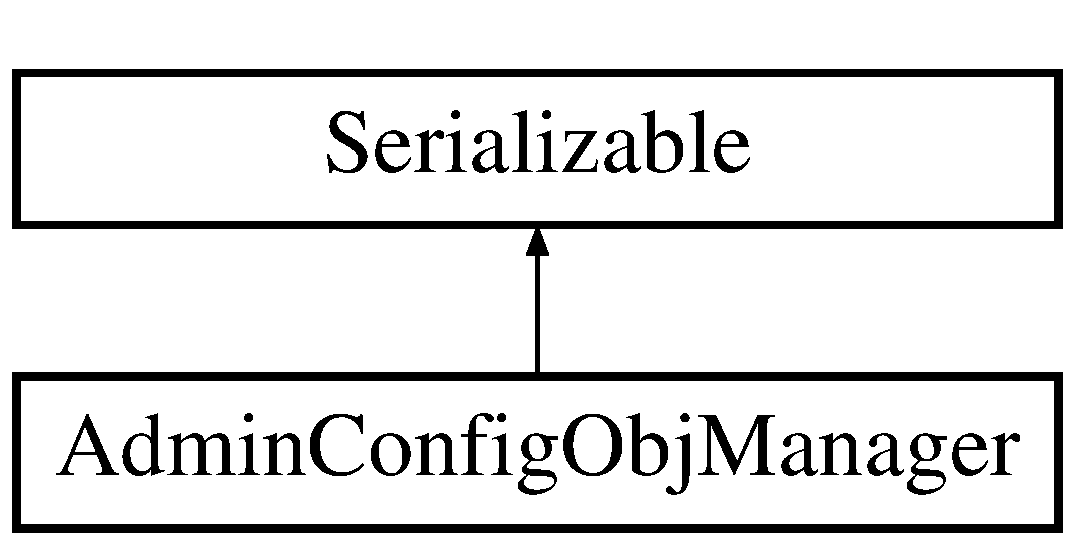
\includegraphics[height=2.000000cm]{classAdminConfigObjManager}
\end{center}
\end{figure}
\subsection*{\-Métodos públicos}
\begin{DoxyCompactItemize}
\item 
\hyperlink{classAdminConfigObjManager_ac1cf996dac14964ef66fa2a58cb203cc}{\-Admin\-Config\-Obj\-Manager} (t\-\_\-\-Objeto tipo, \-Gtk\-::\-Combo\-Box\-Text $\ast$cbtext, \-Gtk\-::\-Entry $\ast$p\-Entry, \-Gtk\-::\-Button $\ast$p\-Aceptar, \-Gtk\-::\-Button $\ast$p\-Guardar\-Cambios, \-Gtk\-::\-Button $\ast$p\-Eliminar, const \-Glib\-::ustring \&def)
\item 
\hyperlink{classAdminConfigObjManager_a0ad7c3b6f6efbd2dc9ed22a10419a262}{$\sim$\-Admin\-Config\-Obj\-Manager} ()
\item 
void \hyperlink{classAdminConfigObjManager_af1ffbc3bf75851e87b596c664769720c}{desconectar} ()
\item 
void \hyperlink{classAdminConfigObjManager_a2c1bd9dab0e7549e07792e77ba639f63}{reconectar} ()
\item 
\hyperlink{classConfigModelo}{\-Config\-Modelo} $\ast$ \hyperlink{classAdminConfigObjManager_a988c37775c19546db9c20d099c3b6cf1}{get\-Modelo} () const 
\item 
\hypertarget{classAdminConfigObjManager_ad110baeb7c0888dcf09bb5d72f1d7e37}{std\-::list$<$ \hyperlink{classTabConfigModelo}{\-Tab\-Config\-Modelo} $\ast$ $>$ {\bfseries get\-Modelos\-Como\-Tabs} ()}\label{classAdminConfigObjManager_ad110baeb7c0888dcf09bb5d72f1d7e37}

\item 
\hypertarget{classAdminConfigObjManager_a7d7fe15793209afad0c51853e778acef}{std\-::list$<$ \hyperlink{classPanelConfigModelo}{\-Panel\-Config\-Modelo} $\ast$ $>$ {\bfseries get\-Modelos\-Como\-Paneles} ()}\label{classAdminConfigObjManager_a7d7fe15793209afad0c51853e778acef}

\item 
\hypertarget{classAdminConfigObjManager_a471986147f5b118b418c350a0f06088c}{sigc\-::signal$<$ void, \*
\hyperlink{classConfigModelo}{\-Config\-Modelo} $\ast$ $>$ {\bfseries signal\-\_\-model\-\_\-changed} ()}\label{classAdminConfigObjManager_a471986147f5b118b418c350a0f06088c}

\item 
\hypertarget{classAdminConfigObjManager_aa1702ac8baace3d410a3379d9acbfb5e}{sigc\-::signal$<$ void, \*
\hyperlink{classConfigModelo}{\-Config\-Modelo} $\ast$ $>$ {\bfseries signal\-\_\-model\-\_\-saved} ()}\label{classAdminConfigObjManager_aa1702ac8baace3d410a3379d9acbfb5e}

\item 
\hypertarget{classAdminConfigObjManager_af50cdd1b684a7170cf35836c80768763}{sigc\-::signal$<$ void, \*
\hyperlink{classConfigModelo}{\-Config\-Modelo} $\ast$ $>$ {\bfseries signal\-\_\-model\-\_\-deleted} ()}\label{classAdminConfigObjManager_af50cdd1b684a7170cf35836c80768763}

\item 
\hypertarget{classAdminConfigObjManager_aa25ec5375405a77449aa2c9b345f42c9}{virtual \hyperlink{classTiXmlElement}{\-Nodo\-Xml} {\bfseries serializar} ()}\label{classAdminConfigObjManager_aa25ec5375405a77449aa2c9b345f42c9}

\item 
\hypertarget{classAdminConfigObjManager_a2b266588c890c4fa828daa716ea5653e}{virtual void {\bfseries deserializar} (const \hyperlink{classTiXmlElement}{\-Nodo\-Xml} \&nodo)}\label{classAdminConfigObjManager_a2b266588c890c4fa828daa716ea5653e}

\end{DoxyCompactItemize}


\subsection{\-Descripción detallada}
\-Clase encargada de manejar la parte de agregado de objetos dinámicos por el admin (pestañas y paneles).

\-Implementa una pequeña factory en base al enum t\-\_\-\-Objeto.

\-Emite las señales\-: -\/signal\-\_\-model\-\_\-changed cuando el modelo que está detrás de la vista cambia. -\/signal\-\_\-model\-\_\-deleted cuando el modelo seleccionado fue eliminado -\/signal\-\_\-model\-\_\-saved cuando el modelo seleccionado guarda sus cambios 

\subsection{\-Documentación del constructor y destructor}
\hypertarget{classAdminConfigObjManager_ac1cf996dac14964ef66fa2a58cb203cc}{\index{\-Admin\-Config\-Obj\-Manager@{\-Admin\-Config\-Obj\-Manager}!\-Admin\-Config\-Obj\-Manager@{\-Admin\-Config\-Obj\-Manager}}
\index{\-Admin\-Config\-Obj\-Manager@{\-Admin\-Config\-Obj\-Manager}!AdminConfigObjManager@{\-Admin\-Config\-Obj\-Manager}}
\subsubsection[{\-Admin\-Config\-Obj\-Manager}]{\setlength{\rightskip}{0pt plus 5cm}{\bf \-Admin\-Config\-Obj\-Manager\-::\-Admin\-Config\-Obj\-Manager} (
\begin{DoxyParamCaption}
\item[{t\-\_\-\-Objeto}]{tipo, }
\item[{\-Gtk\-::\-Combo\-Box\-Text $\ast$}]{cbtext, }
\item[{\-Gtk\-::\-Entry $\ast$}]{p\-Entry, }
\item[{\-Gtk\-::\-Button $\ast$}]{p\-Aceptar, }
\item[{\-Gtk\-::\-Button $\ast$}]{p\-Guardar\-Cambios, }
\item[{\-Gtk\-::\-Button $\ast$}]{p\-Eliminar, }
\item[{const \-Glib\-::ustring \&}]{def}
\end{DoxyParamCaption}
)}}\label{classAdminConfigObjManager_ac1cf996dac14964ef66fa2a58cb203cc}
\-Constructor. \hypertarget{classAdminConfigObjManager_a0ad7c3b6f6efbd2dc9ed22a10419a262}{\index{\-Admin\-Config\-Obj\-Manager@{\-Admin\-Config\-Obj\-Manager}!$\sim$\-Admin\-Config\-Obj\-Manager@{$\sim$\-Admin\-Config\-Obj\-Manager}}
\index{$\sim$\-Admin\-Config\-Obj\-Manager@{$\sim$\-Admin\-Config\-Obj\-Manager}!AdminConfigObjManager@{\-Admin\-Config\-Obj\-Manager}}
\subsubsection[{$\sim$\-Admin\-Config\-Obj\-Manager}]{\setlength{\rightskip}{0pt plus 5cm}{\bf \-Admin\-Config\-Obj\-Manager\-::$\sim$\-Admin\-Config\-Obj\-Manager} (
\begin{DoxyParamCaption}
{}
\end{DoxyParamCaption}
)}}\label{classAdminConfigObjManager_a0ad7c3b6f6efbd2dc9ed22a10419a262}
\-Destructor. \-Libera todos los \hyperlink{classConfigModelo}{\-Config\-Modelo} instanciados en el heap 

\subsection{\-Documentación de las funciones miembro}
\hypertarget{classAdminConfigObjManager_af1ffbc3bf75851e87b596c664769720c}{\index{\-Admin\-Config\-Obj\-Manager@{\-Admin\-Config\-Obj\-Manager}!desconectar@{desconectar}}
\index{desconectar@{desconectar}!AdminConfigObjManager@{\-Admin\-Config\-Obj\-Manager}}
\subsubsection[{desconectar}]{\setlength{\rightskip}{0pt plus 5cm}void {\bf \-Admin\-Config\-Obj\-Manager\-::desconectar} (
\begin{DoxyParamCaption}
{}
\end{DoxyParamCaption}
)}}\label{classAdminConfigObjManager_af1ffbc3bf75851e87b596c664769720c}
\-Desconecta toda conexión con señales de widgets de vista. \hypertarget{classAdminConfigObjManager_a988c37775c19546db9c20d099c3b6cf1}{\index{\-Admin\-Config\-Obj\-Manager@{\-Admin\-Config\-Obj\-Manager}!get\-Modelo@{get\-Modelo}}
\index{get\-Modelo@{get\-Modelo}!AdminConfigObjManager@{\-Admin\-Config\-Obj\-Manager}}
\subsubsection[{get\-Modelo}]{\setlength{\rightskip}{0pt plus 5cm}{\bf \-Config\-Modelo} $\ast$ {\bf \-Admin\-Config\-Obj\-Manager\-::get\-Modelo} (
\begin{DoxyParamCaption}
{}
\end{DoxyParamCaption}
) const}}\label{classAdminConfigObjManager_a988c37775c19546db9c20d099c3b6cf1}
\-Obtener el modelo seleccionado. \begin{DoxyReturn}{\-Devuelve}
puntero al modelo actual 
\end{DoxyReturn}
\hypertarget{classAdminConfigObjManager_a2c1bd9dab0e7549e07792e77ba639f63}{\index{\-Admin\-Config\-Obj\-Manager@{\-Admin\-Config\-Obj\-Manager}!reconectar@{reconectar}}
\index{reconectar@{reconectar}!AdminConfigObjManager@{\-Admin\-Config\-Obj\-Manager}}
\subsubsection[{reconectar}]{\setlength{\rightskip}{0pt plus 5cm}void {\bf \-Admin\-Config\-Obj\-Manager\-::reconectar} (
\begin{DoxyParamCaption}
{}
\end{DoxyParamCaption}
)}}\label{classAdminConfigObjManager_a2c1bd9dab0e7549e07792e77ba639f63}
\-Reconecta las conexiones. 

\-La documentación para esta clase fue generada a partir de los siguientes ficheros\-:\begin{DoxyCompactItemize}
\item 
cliente/\-Modelo/\-Admin\-Config\-Obj\-Manager.\-h\item 
cliente/\-Modelo/\-Admin\-Config\-Obj\-Manager.\-cpp\end{DoxyCompactItemize}

\hypertarget{classAgente}{\section{\-Referencia de la \-Clase \-Agente}
\label{classAgente}\index{\-Agente@{\-Agente}}
}


{\ttfamily \#include $<$\-Agente.\-h$>$}

\subsection*{\-Métodos públicos}
\begin{DoxyCompactItemize}
\item 
\hyperlink{classAgente_a85f3ede45fe8c713306a1b342413c692}{\-Agente} (const std\-::string \&ruta\-Config=\char`\"{}\char`\"{})
\begin{DoxyCompactList}\small\item\em \-Constructor que recive la ruta del archivo de configuracion. \end{DoxyCompactList}\item 
\hypertarget{classAgente_a2c1bbeaa1f77734741b15999f8459871}{void \hyperlink{classAgente_a2c1bbeaa1f77734741b15999f8459871}{cargar\-Desde\-Consola} ()}\label{classAgente_a2c1bbeaa1f77734741b15999f8459871}

\begin{DoxyCompactList}\small\item\em \-Se intenta conectar con el servidor y luego se cargan registros uno por uno. \end{DoxyCompactList}\item 
void \hyperlink{classAgente_a2441654a1842994e9b31a04f66bc6eaf}{cargar\-Desde\-Archivo} (const std\-::string \&ruta\-Datos)
\begin{DoxyCompactList}\small\item\em \-Se intenta conectar con el servidor y luego se cargar los registros directamente desde un archivo. \end{DoxyCompactList}\end{DoxyCompactItemize}


\subsection{\-Descripción detallada}
\-Esta clase cumple el rol completo de un agente. \-Encargandose de enviar registros uno por uno a un \hyperlink{classServidor}{\-Servidor} o enviar \-Registros a travez de \-Archivos. 

\subsection{\-Documentación del constructor y destructor}
\hypertarget{classAgente_a85f3ede45fe8c713306a1b342413c692}{\index{\-Agente@{\-Agente}!\-Agente@{\-Agente}}
\index{\-Agente@{\-Agente}!Agente@{\-Agente}}
\subsubsection[{\-Agente}]{\setlength{\rightskip}{0pt plus 5cm}{\bf \-Agente\-::\-Agente} (
\begin{DoxyParamCaption}
\item[{const std\-::string \&}]{ruta\-Config = {\ttfamily \char`\"{}\char`\"{}}}
\end{DoxyParamCaption}
)}}\label{classAgente_a85f3ede45fe8c713306a1b342413c692}


\-Constructor que recive la ruta del archivo de configuracion. 


\begin{DoxyParams}{\-Parámetros}
{\em ruta\-Config} & string que contiene la ruta del archivo de config. \\
\hline
\end{DoxyParams}


\subsection{\-Documentación de las funciones miembro}
\hypertarget{classAgente_a2441654a1842994e9b31a04f66bc6eaf}{\index{\-Agente@{\-Agente}!cargar\-Desde\-Archivo@{cargar\-Desde\-Archivo}}
\index{cargar\-Desde\-Archivo@{cargar\-Desde\-Archivo}!Agente@{\-Agente}}
\subsubsection[{cargar\-Desde\-Archivo}]{\setlength{\rightskip}{0pt plus 5cm}void {\bf \-Agente\-::cargar\-Desde\-Archivo} (
\begin{DoxyParamCaption}
\item[{const std\-::string \&}]{ruta\-Datos}
\end{DoxyParamCaption}
)}}\label{classAgente_a2441654a1842994e9b31a04f66bc6eaf}


\-Se intenta conectar con el servidor y luego se cargar los registros directamente desde un archivo. 


\begin{DoxyParams}{\-Parámetros}
{\em ruta\-Datos} & string que contiene la ruta del archivo con lo registros a cargar. \\
\hline
\end{DoxyParams}


\-La documentación para esta clase fue generada a partir de los siguientes ficheros\-:\begin{DoxyCompactItemize}
\item 
agente/\-Agente.\-h\item 
agente/\-Agente.\-cpp\end{DoxyCompactItemize}

\hypertarget{classagenteDummy}{\section{\-Referencia de la \-Clase agente\-Dummy}
\label{classagenteDummy}\index{agente\-Dummy@{agente\-Dummy}}
}
\-Diagrama de herencias de agente\-Dummy\begin{figure}[H]
\begin{center}
\leavevmode
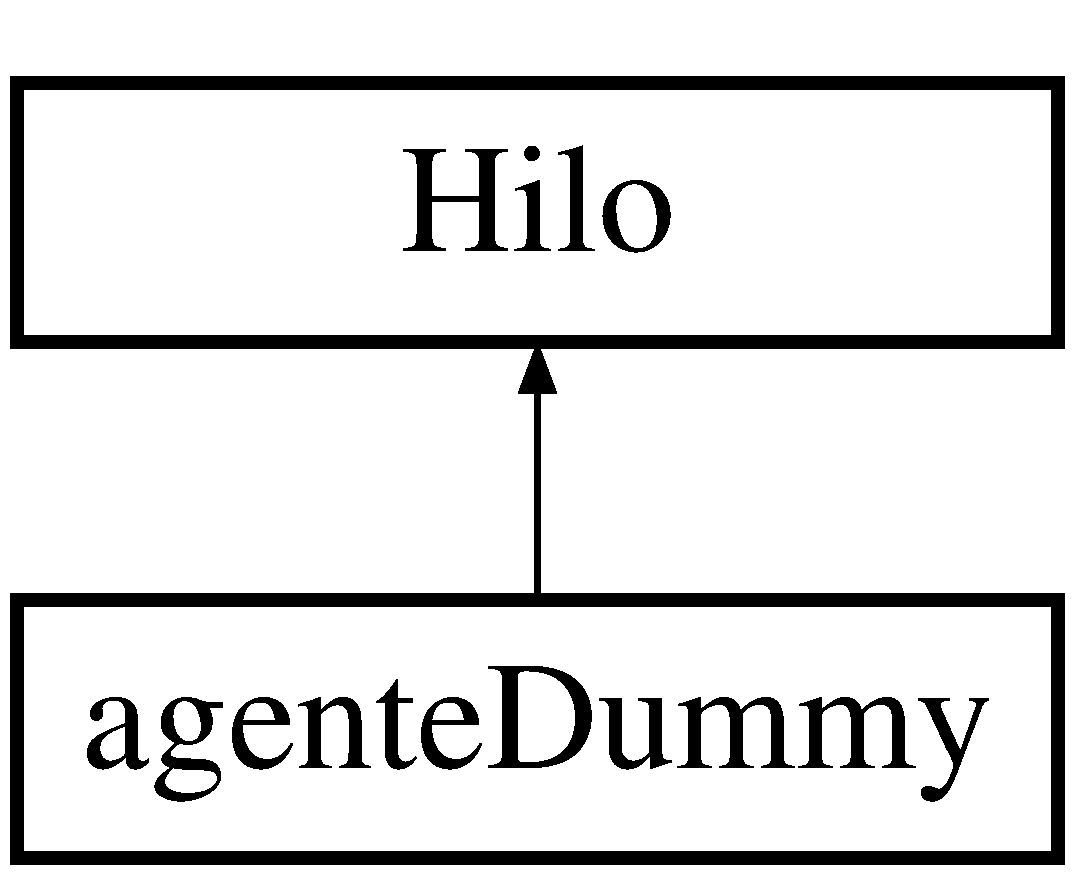
\includegraphics[height=2.000000cm]{classagenteDummy}
\end{center}
\end{figure}
\subsection*{\-Métodos públicos}
\begin{DoxyCompactItemize}
\item 
\hypertarget{classagenteDummy_a9de34fb738e72f3ee2dfa7432cdaf546}{void \hyperlink{classagenteDummy_a9de34fb738e72f3ee2dfa7432cdaf546}{correr} ()}\label{classagenteDummy_a9de34fb738e72f3ee2dfa7432cdaf546}

\begin{DoxyCompactList}\small\item\em \-Metodo virtual puro, que corre cuando se ejecuta el hilo. \end{DoxyCompactList}\end{DoxyCompactItemize}


\-La documentación para esta clase fue generada a partir del siguiente fichero\-:\begin{DoxyCompactItemize}
\item 
servidor/test.\-cpp\end{DoxyCompactItemize}

\hypertarget{classAgenteRemoto}{\section{\-Referencia de la \-Clase \-Agente\-Remoto}
\label{classAgenteRemoto}\index{\-Agente\-Remoto@{\-Agente\-Remoto}}
}


{\ttfamily \#include $<$\-Agente\-Remoto.\-h$>$}

\-Diagrama de herencias de \-Agente\-Remoto\begin{figure}[H]
\begin{center}
\leavevmode
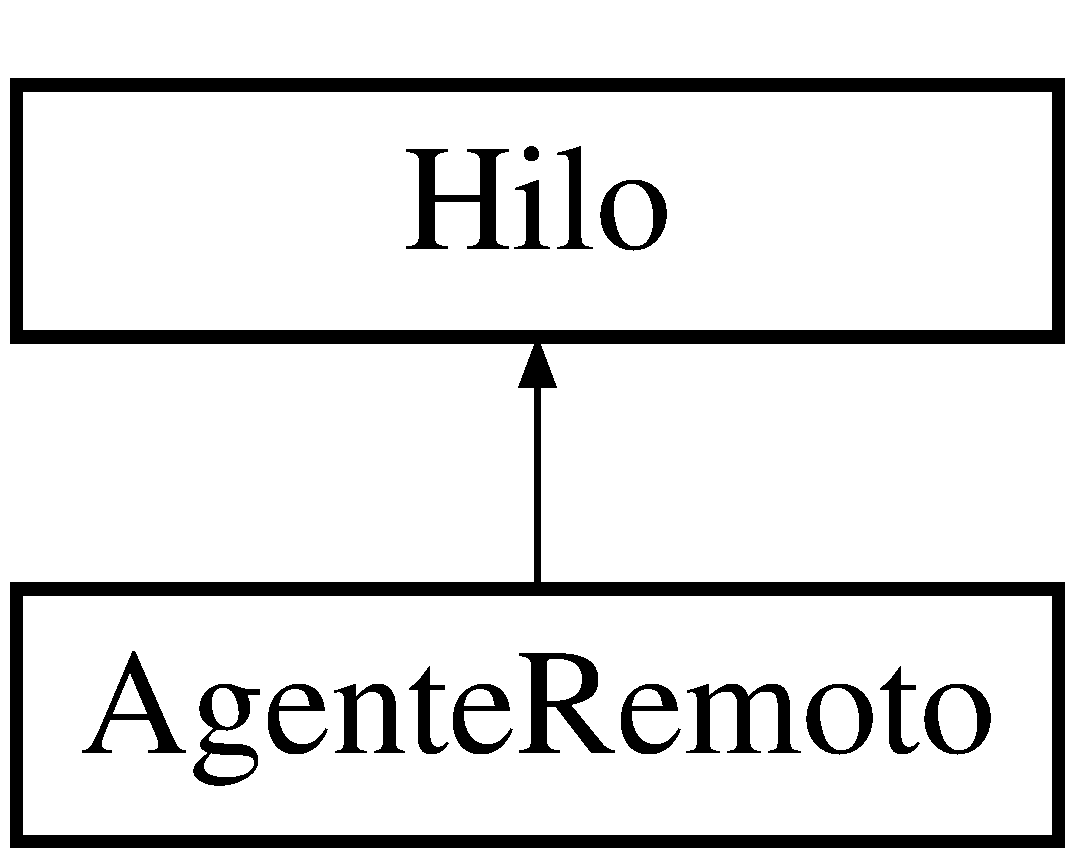
\includegraphics[height=2.000000cm]{classAgenteRemoto}
\end{center}
\end{figure}
\subsection*{\-Métodos públicos}
\begin{DoxyCompactItemize}
\item 
void \hyperlink{classAgenteRemoto_a197fde39c6ee189d9527ac6668d544de}{correr} ()
\item 
void \hyperlink{classAgenteRemoto_ac51c7c596b2e84c9a2881c6e2c0cc345}{detener\-\_\-agente} ()
\item 
void \hyperlink{classAgenteRemoto_a00c67ba1508af5e5ce370c2122fca410}{desconectar\-\_\-agente} ()
\item 
void \hyperlink{classAgenteRemoto_aad964a1ec6c3cac32191e803bc4b4b84}{enviar\-Respuesta} (\hyperlink{classRespuesta}{\-Respuesta} \&r)
\item 
\hyperlink{classAgenteRemoto_a367ab6b1b611c2135e96f9af22697d1b}{\-Agente\-Remoto} (\hyperlink{classSocket}{\-Socket} $\ast$agt, \hyperlink{classResolvedorEntradas}{\-Resolvedor\-Entradas} \&rentr, \hyperlink{classBLQueue}{\-Consultas\-Agentes\-Servidor} \&cons)
\item 
\hyperlink{classAgenteRemoto_a2f741f99a64eaab6094b592b78dfc22d}{$\sim$\-Agente\-Remoto} ()
\end{DoxyCompactItemize}


\subsection{\-Descripción detallada}
\-Esta clase es el proxy del agente. \-A través de la misma el servidor obtendrá entradas de actualización y enviará respuestas. \-Es, a su vez, un productor que alimenta la cola de consultas del servidor. \-Se maneja en un hilo aparte, dado que existe un \hyperlink{classAgenteRemoto}{\-Agente\-Remoto} por agente conectado al servidor. 

\subsection{\-Documentación del constructor y destructor}
\hypertarget{classAgenteRemoto_a367ab6b1b611c2135e96f9af22697d1b}{\index{\-Agente\-Remoto@{\-Agente\-Remoto}!\-Agente\-Remoto@{\-Agente\-Remoto}}
\index{\-Agente\-Remoto@{\-Agente\-Remoto}!AgenteRemoto@{\-Agente\-Remoto}}
\subsubsection[{\-Agente\-Remoto}]{\setlength{\rightskip}{0pt plus 5cm}{\bf \-Agente\-Remoto\-::\-Agente\-Remoto} (
\begin{DoxyParamCaption}
\item[{{\bf \-Socket} $\ast$}]{agt, }
\item[{{\bf \-Resolvedor\-Entradas} \&}]{rentr, }
\item[{{\bf \-Consultas\-Agentes\-Servidor} \&}]{cons}
\end{DoxyParamCaption}
)}}\label{classAgenteRemoto_a367ab6b1b611c2135e96f9af22697d1b}
\-Constructor del agente remoto. 
\begin{DoxyParams}{\-Parámetros}
{\em agt} & \-El socket activo conectado con el servidor. \\
\hline
{\em rentr} & \-Objeto que sea capaz de resolver entradas. \\
\hline
{\em cons} & \-Cola de consultas de agentes del servidor. \\
\hline
\end{DoxyParams}
\hypertarget{classAgenteRemoto_a2f741f99a64eaab6094b592b78dfc22d}{\index{\-Agente\-Remoto@{\-Agente\-Remoto}!$\sim$\-Agente\-Remoto@{$\sim$\-Agente\-Remoto}}
\index{$\sim$\-Agente\-Remoto@{$\sim$\-Agente\-Remoto}!AgenteRemoto@{\-Agente\-Remoto}}
\subsubsection[{$\sim$\-Agente\-Remoto}]{\setlength{\rightskip}{0pt plus 5cm}{\bf \-Agente\-Remoto\-::$\sim$\-Agente\-Remoto} (
\begin{DoxyParamCaption}
{}
\end{DoxyParamCaption}
)}}\label{classAgenteRemoto_a2f741f99a64eaab6094b592b78dfc22d}
\-Destructor de agente remoto. \-Si esta corriendo, lo detiene. \-Si esta conectado, lo desconecta 

\subsection{\-Documentación de las funciones miembro}
\hypertarget{classAgenteRemoto_a197fde39c6ee189d9527ac6668d544de}{\index{\-Agente\-Remoto@{\-Agente\-Remoto}!correr@{correr}}
\index{correr@{correr}!AgenteRemoto@{\-Agente\-Remoto}}
\subsubsection[{correr}]{\setlength{\rightskip}{0pt plus 5cm}void {\bf \-Agente\-Remoto\-::correr} (
\begin{DoxyParamCaption}
{}
\end{DoxyParamCaption}
)\hspace{0.3cm}{\ttfamily  \mbox{[}virtual\mbox{]}}}}\label{classAgenteRemoto_a197fde39c6ee189d9527ac6668d544de}
\-Método que se ejecuta mientras esté en ejecucion el hilo. \-Es el encargado de recibir elementos del socket y encolarlos para que responda el servidor. 

\-Implementa \hyperlink{classHilo_a187b055e3504487a6bb64340fac2c70d}{\-Hilo}.

\hypertarget{classAgenteRemoto_a00c67ba1508af5e5ce370c2122fca410}{\index{\-Agente\-Remoto@{\-Agente\-Remoto}!desconectar\-\_\-agente@{desconectar\-\_\-agente}}
\index{desconectar\-\_\-agente@{desconectar\-\_\-agente}!AgenteRemoto@{\-Agente\-Remoto}}
\subsubsection[{desconectar\-\_\-agente}]{\setlength{\rightskip}{0pt plus 5cm}void {\bf \-Agente\-Remoto\-::desconectar\-\_\-agente} (
\begin{DoxyParamCaption}
{}
\end{DoxyParamCaption}
)}}\label{classAgenteRemoto_a00c67ba1508af5e5ce370c2122fca410}
\-Desconecta el socket del agente remoto. \hypertarget{classAgenteRemoto_ac51c7c596b2e84c9a2881c6e2c0cc345}{\index{\-Agente\-Remoto@{\-Agente\-Remoto}!detener\-\_\-agente@{detener\-\_\-agente}}
\index{detener\-\_\-agente@{detener\-\_\-agente}!AgenteRemoto@{\-Agente\-Remoto}}
\subsubsection[{detener\-\_\-agente}]{\setlength{\rightskip}{0pt plus 5cm}void {\bf \-Agente\-Remoto\-::detener\-\_\-agente} (
\begin{DoxyParamCaption}
{}
\end{DoxyParamCaption}
)}}\label{classAgenteRemoto_ac51c7c596b2e84c9a2881c6e2c0cc345}
\-Detiene la ejecución del agente remoto, sin cerrar el hilo. \hypertarget{classAgenteRemoto_aad964a1ec6c3cac32191e803bc4b4b84}{\index{\-Agente\-Remoto@{\-Agente\-Remoto}!enviar\-Respuesta@{enviar\-Respuesta}}
\index{enviar\-Respuesta@{enviar\-Respuesta}!AgenteRemoto@{\-Agente\-Remoto}}
\subsubsection[{enviar\-Respuesta}]{\setlength{\rightskip}{0pt plus 5cm}void {\bf \-Agente\-Remoto\-::enviar\-Respuesta} (
\begin{DoxyParamCaption}
\item[{{\bf \-Respuesta} \&}]{r}
\end{DoxyParamCaption}
)}}\label{classAgenteRemoto_aad964a1ec6c3cac32191e803bc4b4b84}
\-Envía la respuesta obtenida del servidor al agente. 

\-La documentación para esta clase fue generada a partir de los siguientes ficheros\-:\begin{DoxyCompactItemize}
\item 
servidor/servidor/\-Agente\-Remoto.\-h\item 
servidor/servidor/\-Agente\-Remoto.\-cpp\end{DoxyCompactItemize}

\hypertarget{classArchivoConfiguracion}{\section{\-Referencia de la \-Clase \-Archivo\-Configuracion}
\label{classArchivoConfiguracion}\index{\-Archivo\-Configuracion@{\-Archivo\-Configuracion}}
}


{\ttfamily \#include $<$\-Archivo\-Configuracion.\-h$>$}

\subsection*{\-Tipos públicos}
\begin{DoxyCompactItemize}
\item 
\hypertarget{classArchivoConfiguracion_ab833c19535774fe9d0221c7168ee76be}{typedef std\-::map$<$ std\-::string, \*
std\-::string $>$\-::iterator {\bfseries iterator}}\label{classArchivoConfiguracion_ab833c19535774fe9d0221c7168ee76be}

\end{DoxyCompactItemize}
\subsection*{\-Métodos públicos}
\begin{DoxyCompactItemize}
\item 
std\-::string \hyperlink{classArchivoConfiguracion_a95768ee9e7dbbbfe5569bc2184af3ee8}{obtener\-Atributo} (std\-::string \&name)
\item 
std\-::string \hyperlink{classArchivoConfiguracion_ad6205cb38e5a6453ef98a772c4e198dd}{obtener\-Atributo} (char $\ast$nombre)
\item 
void \hyperlink{classArchivoConfiguracion_a197987be642dd81cb57d6f96cbd08873}{setear\-Atributo} (std\-::string \&nom, std\-::string \&valor)
\item 
\hypertarget{classArchivoConfiguracion_adf342e6c4d4dc3aa48c08f8b623a7ac1}{iterator {\bfseries begin} ()}\label{classArchivoConfiguracion_adf342e6c4d4dc3aa48c08f8b623a7ac1}

\item 
\hypertarget{classArchivoConfiguracion_a38b2a659a848866e48b237a0edefede5}{iterator {\bfseries end} ()}\label{classArchivoConfiguracion_a38b2a659a848866e48b237a0edefede5}

\item 
\hyperlink{classArchivoConfiguracion_acee8a865caeee4ab8dad8e799f776717}{\-Archivo\-Configuracion} (const char $\ast$ruta=\-R\-U\-T\-A)
\item 
\hyperlink{classArchivoConfiguracion_a18138422c075e0090c98978089ac91b0}{$\sim$\-Archivo\-Configuracion} ()
\end{DoxyCompactItemize}


\subsection{\-Descripción detallada}
\-Es una clase de archivo que contiene atributos levantados de un archivo de texto. \-El archivo a levantar se encuentra encriptado. \-Nota\-: esta clase no es thread-\/safe. 

\subsection{\-Documentación del constructor y destructor}
\hypertarget{classArchivoConfiguracion_acee8a865caeee4ab8dad8e799f776717}{\index{\-Archivo\-Configuracion@{\-Archivo\-Configuracion}!\-Archivo\-Configuracion@{\-Archivo\-Configuracion}}
\index{\-Archivo\-Configuracion@{\-Archivo\-Configuracion}!ArchivoConfiguracion@{\-Archivo\-Configuracion}}
\subsubsection[{\-Archivo\-Configuracion}]{\setlength{\rightskip}{0pt plus 5cm}{\bf \-Archivo\-Configuracion\-::\-Archivo\-Configuracion} (
\begin{DoxyParamCaption}
\item[{const char $\ast$}]{ruta = {\ttfamily \-R\-U\-T\-A}}
\end{DoxyParamCaption}
)\hspace{0.3cm}{\ttfamily  \mbox{[}explicit\mbox{]}}}}\label{classArchivoConfiguracion_acee8a865caeee4ab8dad8e799f776717}
\-Si el archivo no existe, no levanta ningun tipo de excepcion \hypertarget{classArchivoConfiguracion_a18138422c075e0090c98978089ac91b0}{\index{\-Archivo\-Configuracion@{\-Archivo\-Configuracion}!$\sim$\-Archivo\-Configuracion@{$\sim$\-Archivo\-Configuracion}}
\index{$\sim$\-Archivo\-Configuracion@{$\sim$\-Archivo\-Configuracion}!ArchivoConfiguracion@{\-Archivo\-Configuracion}}
\subsubsection[{$\sim$\-Archivo\-Configuracion}]{\setlength{\rightskip}{0pt plus 5cm}{\bf \-Archivo\-Configuracion\-::$\sim$\-Archivo\-Configuracion} (
\begin{DoxyParamCaption}
{}
\end{DoxyParamCaption}
)}}\label{classArchivoConfiguracion_a18138422c075e0090c98978089ac91b0}
\-En el destructor es que se persisten los cambios del archivo 

\subsection{\-Documentación de las funciones miembro}
\hypertarget{classArchivoConfiguracion_a95768ee9e7dbbbfe5569bc2184af3ee8}{\index{\-Archivo\-Configuracion@{\-Archivo\-Configuracion}!obtener\-Atributo@{obtener\-Atributo}}
\index{obtener\-Atributo@{obtener\-Atributo}!ArchivoConfiguracion@{\-Archivo\-Configuracion}}
\subsubsection[{obtener\-Atributo}]{\setlength{\rightskip}{0pt plus 5cm}std\-::string {\bf \-Archivo\-Configuracion\-::obtener\-Atributo} (
\begin{DoxyParamCaption}
\item[{std\-::string \&}]{name}
\end{DoxyParamCaption}
)}}\label{classArchivoConfiguracion_a95768ee9e7dbbbfe5569bc2184af3ee8}
\-Devuelve el atributo asociado \hypertarget{classArchivoConfiguracion_ad6205cb38e5a6453ef98a772c4e198dd}{\index{\-Archivo\-Configuracion@{\-Archivo\-Configuracion}!obtener\-Atributo@{obtener\-Atributo}}
\index{obtener\-Atributo@{obtener\-Atributo}!ArchivoConfiguracion@{\-Archivo\-Configuracion}}
\subsubsection[{obtener\-Atributo}]{\setlength{\rightskip}{0pt plus 5cm}std\-::string {\bf \-Archivo\-Configuracion\-::obtener\-Atributo} (
\begin{DoxyParamCaption}
\item[{char $\ast$}]{nombre}
\end{DoxyParamCaption}
)}}\label{classArchivoConfiguracion_ad6205cb38e5a6453ef98a772c4e198dd}
\begin{DoxySeeAlso}{\-Ver también}
\hyperlink{classArchivoConfiguracion_a95768ee9e7dbbbfe5569bc2184af3ee8}{obtener\-Atributo} 
\end{DoxySeeAlso}
\hypertarget{classArchivoConfiguracion_a197987be642dd81cb57d6f96cbd08873}{\index{\-Archivo\-Configuracion@{\-Archivo\-Configuracion}!setear\-Atributo@{setear\-Atributo}}
\index{setear\-Atributo@{setear\-Atributo}!ArchivoConfiguracion@{\-Archivo\-Configuracion}}
\subsubsection[{setear\-Atributo}]{\setlength{\rightskip}{0pt plus 5cm}void {\bf \-Archivo\-Configuracion\-::setear\-Atributo} (
\begin{DoxyParamCaption}
\item[{std\-::string \&}]{nom, }
\item[{std\-::string \&}]{valor}
\end{DoxyParamCaption}
)}}\label{classArchivoConfiguracion_a197987be642dd81cb57d6f96cbd08873}
\-Setea el atributo \char`\"{}nom\char`\"{} con \char`\"{}valor\char`\"{} 

\-La documentación para esta clase fue generada a partir de los siguientes ficheros\-:\begin{DoxyCompactItemize}
\item 
comun/\-Archivo\-Configuracion.\-h\item 
comun/\-Archivo\-Configuracion.\-cpp\end{DoxyCompactItemize}

\hypertarget{classArchivoDeDatos}{\section{\-Referencia de la \-Clase \-Archivo\-De\-Datos}
\label{classArchivoDeDatos}\index{\-Archivo\-De\-Datos@{\-Archivo\-De\-Datos}}
}


{\ttfamily \#include $<$\-Archivo\-De\-Datos.\-h$>$}

\subsection*{\-Métodos públicos}
\begin{DoxyCompactItemize}
\item 
\hypertarget{classArchivoDeDatos_a7388ffa446c1c16388367bb7a485d791}{\hyperlink{classArchivoDeDatos_a7388ffa446c1c16388367bb7a485d791}{\-Archivo\-De\-Datos} (const std\-::string \&ruta)}\label{classArchivoDeDatos_a7388ffa446c1c16388367bb7a485d791}

\begin{DoxyCompactList}\small\item\em \-Constructor que recibe la ruta del archivo de datos. \end{DoxyCompactList}\item 
std\-::string \hyperlink{classArchivoDeDatos_acb8bffaaacd961744a0f450ab8e3924a}{obtener\-Registro} (\-Id\-\_\-\-Registro id)
\begin{DoxyCompactList}\small\item\em \-Obtiene el registro con numero \char`\"{}id\char`\"{} del archivo. \end{DoxyCompactList}\item 
\-Id\-\_\-\-Registro \hyperlink{classArchivoDeDatos_af678ef7076885d11cefb0a21f2239526}{guardar\-Registro} (const std\-::string \&registro)
\begin{DoxyCompactList}\small\item\em \-Guarda el registro en el archivo. \end{DoxyCompactList}\item 
size\-\_\-t \hyperlink{classArchivoDeDatos_a62e7765b4d6dc435fdf760ceb7a12cc4}{cantidad\-Registros} () const 
\begin{DoxyCompactList}\small\item\em \-Retorna la cantidad de registros que estan guardados en el archivo. \end{DoxyCompactList}\item 
\hypertarget{classArchivoDeDatos_a42079c29fd3c465a1ba83693795e7341}{void \hyperlink{classArchivoDeDatos_a42079c29fd3c465a1ba83693795e7341}{borrar\-Datos} ()}\label{classArchivoDeDatos_a42079c29fd3c465a1ba83693795e7341}

\begin{DoxyCompactList}\small\item\em \-Borra todo el contenido de los datos. \end{DoxyCompactList}\end{DoxyCompactItemize}


\subsection{\-Descripción detallada}
\-Esta clase es la encargada de almacenar todo tipo de registros guardándolos en disco, permitiendo acceder a estos a partir de su id de registro. 

\subsection{\-Documentación de las funciones miembro}
\hypertarget{classArchivoDeDatos_a62e7765b4d6dc435fdf760ceb7a12cc4}{\index{\-Archivo\-De\-Datos@{\-Archivo\-De\-Datos}!cantidad\-Registros@{cantidad\-Registros}}
\index{cantidad\-Registros@{cantidad\-Registros}!ArchivoDeDatos@{\-Archivo\-De\-Datos}}
\subsubsection[{cantidad\-Registros}]{\setlength{\rightskip}{0pt plus 5cm}size\-\_\-t {\bf \-Archivo\-De\-Datos\-::cantidad\-Registros} (
\begin{DoxyParamCaption}
{}
\end{DoxyParamCaption}
) const}}\label{classArchivoDeDatos_a62e7765b4d6dc435fdf760ceb7a12cc4}


\-Retorna la cantidad de registros que estan guardados en el archivo. 

\begin{DoxyReturn}{\-Devuelve}
cantidad de registros actual. 
\end{DoxyReturn}
\hypertarget{classArchivoDeDatos_af678ef7076885d11cefb0a21f2239526}{\index{\-Archivo\-De\-Datos@{\-Archivo\-De\-Datos}!guardar\-Registro@{guardar\-Registro}}
\index{guardar\-Registro@{guardar\-Registro}!ArchivoDeDatos@{\-Archivo\-De\-Datos}}
\subsubsection[{guardar\-Registro}]{\setlength{\rightskip}{0pt plus 5cm}\-Id\-\_\-\-Registro {\bf \-Archivo\-De\-Datos\-::guardar\-Registro} (
\begin{DoxyParamCaption}
\item[{const std\-::string \&}]{registro}
\end{DoxyParamCaption}
)}}\label{classArchivoDeDatos_af678ef7076885d11cefb0a21f2239526}


\-Guarda el registro en el archivo. 


\begin{DoxyParams}{\-Parámetros}
{\em registro} & que se almacenara en el archivo \\
\hline
\end{DoxyParams}
\begin{DoxyReturn}{\-Devuelve}
identificador del registro guardado 
\end{DoxyReturn}
\hypertarget{classArchivoDeDatos_acb8bffaaacd961744a0f450ab8e3924a}{\index{\-Archivo\-De\-Datos@{\-Archivo\-De\-Datos}!obtener\-Registro@{obtener\-Registro}}
\index{obtener\-Registro@{obtener\-Registro}!ArchivoDeDatos@{\-Archivo\-De\-Datos}}
\subsubsection[{obtener\-Registro}]{\setlength{\rightskip}{0pt plus 5cm}std\-::string {\bf \-Archivo\-De\-Datos\-::obtener\-Registro} (
\begin{DoxyParamCaption}
\item[{\-Id\-\_\-\-Registro}]{id}
\end{DoxyParamCaption}
)}}\label{classArchivoDeDatos_acb8bffaaacd961744a0f450ab8e3924a}


\-Obtiene el registro con numero \char`\"{}id\char`\"{} del archivo. 


\begin{DoxyParams}{\-Parámetros}
{\em id} & identificador del registro a recuperar \\
\hline
\end{DoxyParams}
\begin{DoxyReturn}{\-Devuelve}
string que contiene el registro completo recuperado 
\end{DoxyReturn}


\-La documentación para esta clase fue generada a partir de los siguientes ficheros\-:\begin{DoxyCompactItemize}
\item 
servidor/\-Motor\-De\-Consultas/\-Archivo\-De\-Datos.\-h\item 
servidor/\-Motor\-De\-Consultas/\-Archivo\-De\-Datos.\-cpp\end{DoxyCompactItemize}

\hypertarget{classArea}{\section{\-Referencia de la \-Clase \-Area}
\label{classArea}\index{\-Area@{\-Area}}
}


{\ttfamily \#include $<$\-Area.\-h$>$}

\-Diagrama de herencias de \-Area\begin{figure}[H]
\begin{center}
\leavevmode
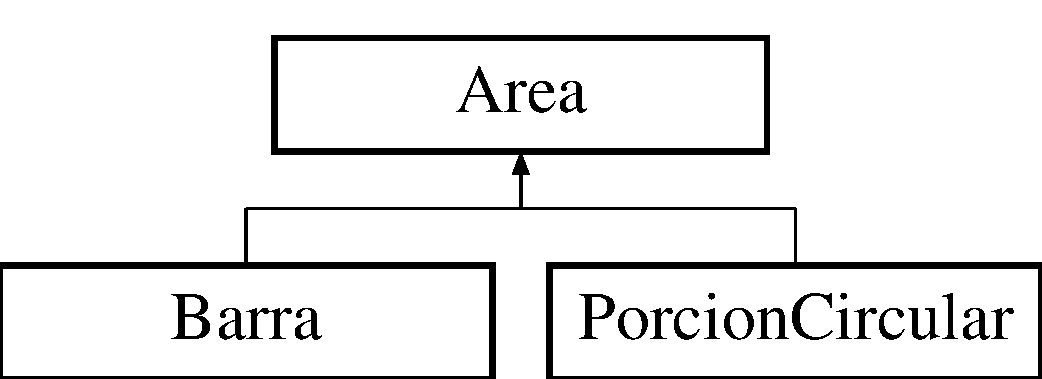
\includegraphics[height=2.000000cm]{classArea}
\end{center}
\end{figure}
\subsection*{\-Métodos públicos}
\begin{DoxyCompactItemize}
\item 
\hyperlink{classArea_a5731b69e91544f031d0b3704397d6fc7}{\-Area} (const \hyperlink{classHecho}{\-Hecho} \&dato, double maximo, unsigned i, double offset)
\item 
\hyperlink{classArea_ace0975982b61a16746c564a0d43a4cc8}{$\sim$\-Area} ()
\item 
\hypertarget{classArea_a90c09de98eae75693b9c79343ca297ca}{const \-Glib\-::ustring \& {\bfseries get\-Etiqueta} () const }\label{classArea_a90c09de98eae75693b9c79343ca297ca}

\item 
\hypertarget{classArea_a2db89df7aded80c028a412221b237491}{virtual const double $\ast$ {\bfseries get\-Color} () const }\label{classArea_a2db89df7aded80c028a412221b237491}

\item 
virtual void \hyperlink{classArea_a95274f96ffa5525307f0a00d074047fb}{dibujar} (\-Cairo\-::\-Ref\-Ptr$<$ \-Cairo\-::\-Context $>$ \&ctx)=0
\item 
virtual bool \hyperlink{classArea_a4158f8c72ff8c67b5d1de00aa9691e90}{fue\-Clickeada} (double x, double y)=0
\item 
virtual double \hyperlink{classArea_ac8a3293cc9ba5678997e9cb0b4a142f9}{get\-Avance} ()=0
\item 
\hypertarget{classArea_a5955ad0781f9cf9bee7e845a7d1dffee}{void {\bfseries set\-Seleccionada} (bool selec)}\label{classArea_a5955ad0781f9cf9bee7e845a7d1dffee}

\item 
virtual std\-::string \hyperlink{classArea_a1934f44c890ca764b7e47dba984a32d5}{get\-Info} ()=0
\end{DoxyCompactItemize}
\subsection*{\-Métodos protegidos}
\begin{DoxyCompactItemize}
\item 
\hypertarget{classArea_a0ca36f43b54962940236f35dd451999f}{void {\bfseries set\-\_\-line\-\_\-width} (\-Cairo\-::\-Ref\-Ptr$<$ \-Cairo\-::\-Context $>$ \&ctx)}\label{classArea_a0ca36f43b54962940236f35dd451999f}

\end{DoxyCompactItemize}
\subsection*{\-Atributos protegidos}
\begin{DoxyCompactItemize}
\item 
\hypertarget{classArea_ac254039e6cdfea6921e15ea66c3fa748}{\hyperlink{classHecho}{\-Hecho} {\bfseries dato}}\label{classArea_ac254039e6cdfea6921e15ea66c3fa748}

\item 
\hypertarget{classArea_aaec8b27b607b17ec509c35d4157271b5}{double {\bfseries max}}\label{classArea_aaec8b27b607b17ec509c35d4157271b5}

\item 
\hypertarget{classArea_a690c7dd341ef34aa9b81e9860732eba5}{double {\bfseries color} \mbox{[}4\mbox{]}}\label{classArea_a690c7dd341ef34aa9b81e9860732eba5}

\item 
\hypertarget{classArea_a22f6ce0774ab2cd976ab40edfdff67c9}{double {\bfseries offset}}\label{classArea_a22f6ce0774ab2cd976ab40edfdff67c9}

\end{DoxyCompactItemize}


\subsection{\-Descripción detallada}
\-Clase abstracta que comprende comportamiento común a toda área de un gŕafico, como la capacidad de responder si un click del mouse cayó sobre ella, retornar una string informativa y, el más importante, dibujarse. 

\subsection{\-Documentación del constructor y destructor}
\hypertarget{classArea_a5731b69e91544f031d0b3704397d6fc7}{\index{\-Area@{\-Area}!\-Area@{\-Area}}
\index{\-Area@{\-Area}!Area@{\-Area}}
\subsubsection[{\-Area}]{\setlength{\rightskip}{0pt plus 5cm}{\bf \-Area\-::\-Area} (
\begin{DoxyParamCaption}
\item[{const {\bf \-Hecho} \&}]{dato, }
\item[{double}]{maximo, }
\item[{unsigned}]{i, }
\item[{double}]{offset}
\end{DoxyParamCaption}
)}}\label{classArea_a5731b69e91544f031d0b3704397d6fc7}
\-Constructor. 
\begin{DoxyParams}{\-Parámetros}
{\em dato} & aquello que representará el área \\
\hline
{\em maximo} & el valor máximo encontrado \\
\hline
{\em i} & número de porción (esto es meramente por el color) \\
\hline
{\em offset} & desplazamiento del área \\
\hline
\end{DoxyParams}
\hypertarget{classArea_ace0975982b61a16746c564a0d43a4cc8}{\index{\-Area@{\-Area}!$\sim$\-Area@{$\sim$\-Area}}
\index{$\sim$\-Area@{$\sim$\-Area}!Area@{\-Area}}
\subsubsection[{$\sim$\-Area}]{\setlength{\rightskip}{0pt plus 5cm}{\bf \-Area\-::$\sim$\-Area} (
\begin{DoxyParamCaption}
{}
\end{DoxyParamCaption}
)}}\label{classArea_ace0975982b61a16746c564a0d43a4cc8}
\-Destructor. 

\subsection{\-Documentación de las funciones miembro}
\hypertarget{classArea_a95274f96ffa5525307f0a00d074047fb}{\index{\-Area@{\-Area}!dibujar@{dibujar}}
\index{dibujar@{dibujar}!Area@{\-Area}}
\subsubsection[{dibujar}]{\setlength{\rightskip}{0pt plus 5cm}virtual void {\bf \-Area\-::dibujar} (
\begin{DoxyParamCaption}
\item[{\-Cairo\-::\-Ref\-Ptr$<$ \-Cairo\-::\-Context $>$ \&}]{ctx}
\end{DoxyParamCaption}
)\hspace{0.3cm}{\ttfamily  \mbox{[}pure virtual\mbox{]}}}}\label{classArea_a95274f96ffa5525307f0a00d074047fb}
\-Dibuja el área. 
\begin{DoxyParams}{\-Parámetros}
{\em ctx} & contexto sobre el que se dibuja \\
\hline
\end{DoxyParams}


\-Implementado en \hyperlink{classPorcionCircular_a88b4c95825dd491a343576dbe6e00496}{\-Porcion\-Circular} y \hyperlink{classBarra_af5dc4f34b2441270ad906de2d8a745d0}{\-Barra}.

\hypertarget{classArea_a4158f8c72ff8c67b5d1de00aa9691e90}{\index{\-Area@{\-Area}!fue\-Clickeada@{fue\-Clickeada}}
\index{fue\-Clickeada@{fue\-Clickeada}!Area@{\-Area}}
\subsubsection[{fue\-Clickeada}]{\setlength{\rightskip}{0pt plus 5cm}virtual bool {\bf \-Area\-::fue\-Clickeada} (
\begin{DoxyParamCaption}
\item[{double}]{x, }
\item[{double}]{y}
\end{DoxyParamCaption}
)\hspace{0.3cm}{\ttfamily  \mbox{[}pure virtual\mbox{]}}}}\label{classArea_a4158f8c72ff8c67b5d1de00aa9691e90}
\-Evalúa si el mouse está posado sobre el área. 
\begin{DoxyParams}{\-Parámetros}
{\em x} & posición x del mouse en la ventana, normalizada \\
\hline
{\em y} & posición y del mouse en la ventana, normalizada \\
\hline
\end{DoxyParams}
\begin{DoxyReturn}{\-Devuelve}
true o false, según la posición pertenece al área 
\end{DoxyReturn}


\-Implementado en \hyperlink{classPorcionCircular_aa39b24dbc7966b5b44c65e85eb389a71}{\-Porcion\-Circular} y \hyperlink{classBarra_a5d04d0e7c196327c0b58409c7854d5ca}{\-Barra}.

\hypertarget{classArea_ac8a3293cc9ba5678997e9cb0b4a142f9}{\index{\-Area@{\-Area}!get\-Avance@{get\-Avance}}
\index{get\-Avance@{get\-Avance}!Area@{\-Area}}
\subsubsection[{get\-Avance}]{\setlength{\rightskip}{0pt plus 5cm}virtual double {\bf \-Area\-::get\-Avance} (
\begin{DoxyParamCaption}
{}
\end{DoxyParamCaption}
)\hspace{0.3cm}{\ttfamily  \mbox{[}pure virtual\mbox{]}}}}\label{classArea_ac8a3293cc9ba5678997e9cb0b4a142f9}
\-Obtener el offset nuevo. \begin{DoxyReturn}{\-Devuelve}
posición siguiente a dibujar un área 
\end{DoxyReturn}


\-Implementado en \hyperlink{classPorcionCircular_ac92b4a76e251f16006f06419354f28d7}{\-Porcion\-Circular} y \hyperlink{classBarra_a705b42ca3d507c0f02786065c889f199}{\-Barra}.

\hypertarget{classArea_a1934f44c890ca764b7e47dba984a32d5}{\index{\-Area@{\-Area}!get\-Info@{get\-Info}}
\index{get\-Info@{get\-Info}!Area@{\-Area}}
\subsubsection[{get\-Info}]{\setlength{\rightskip}{0pt plus 5cm}virtual std\-::string {\bf \-Area\-::get\-Info} (
\begin{DoxyParamCaption}
{}
\end{DoxyParamCaption}
)\hspace{0.3cm}{\ttfamily  \mbox{[}pure virtual\mbox{]}}}}\label{classArea_a1934f44c890ca764b7e47dba984a32d5}
\-Información sobre el área. \begin{DoxyReturn}{\-Devuelve}
string para tooltip 
\end{DoxyReturn}


\-Implementado en \hyperlink{classPorcionCircular_ae19f4777d0f9b0ed31e9305783e34a40}{\-Porcion\-Circular} y \hyperlink{classBarra_a5d8b121357bdeec02ab3cf46e95b740c}{\-Barra}.



\-La documentación para esta clase fue generada a partir de los siguientes ficheros\-:\begin{DoxyCompactItemize}
\item 
cliente/\-Vista/\-Area.\-h\item 
cliente/\-Vista/\-Area.\-cpp\end{DoxyCompactItemize}

\hypertarget{classBarra}{\section{\-Referencia de la \-Clase \-Barra}
\label{classBarra}\index{\-Barra@{\-Barra}}
}


{\ttfamily \#include $<$\-Barra.\-h$>$}

\-Diagrama de herencias de \-Barra\begin{figure}[H]
\begin{center}
\leavevmode
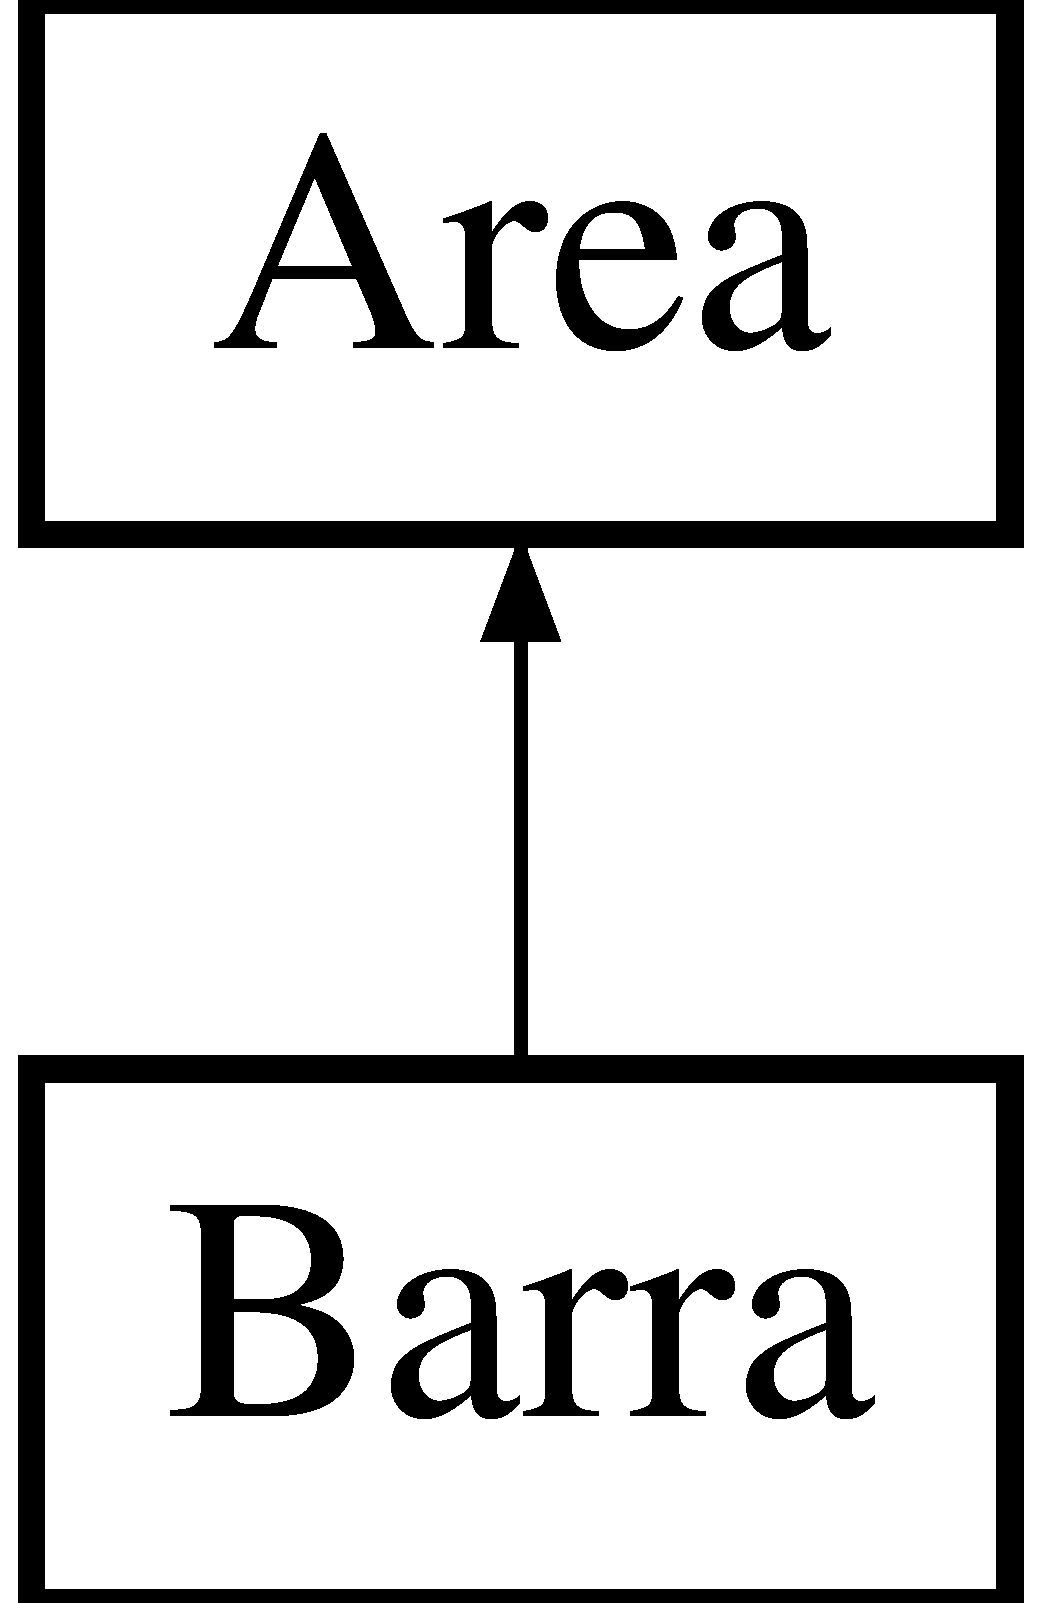
\includegraphics[height=2.000000cm]{classBarra}
\end{center}
\end{figure}
\subsection*{\-Métodos públicos}
\begin{DoxyCompactItemize}
\item 
\hyperlink{classBarra_a8edaf9bde1490cb349c50a1665c32193}{\-Barra} (const \hyperlink{classHecho}{\-Hecho} \&dato, double maximo, unsigned i, double offset, double separacion, double ancho)
\item 
\hyperlink{classBarra_a0d8469e11d2382e0808879f4f500062f}{$\sim$\-Barra} ()
\item 
void \hyperlink{classBarra_af5dc4f34b2441270ad906de2d8a745d0}{dibujar} (\-Cairo\-::\-Ref\-Ptr$<$ \-Cairo\-::\-Context $>$ \&ctx)
\item 
bool \hyperlink{classBarra_a5d04d0e7c196327c0b58409c7854d5ca}{fue\-Clickeada} (double x, double y)
\item 
double \hyperlink{classBarra_a705b42ca3d507c0f02786065c889f199}{get\-Avance} ()
\item 
std\-::string \hyperlink{classBarra_a5d8b121357bdeec02ab3cf46e95b740c}{get\-Info} ()
\end{DoxyCompactItemize}


\subsection{\-Descripción detallada}
\-Clase concreta que representa una barra de un gráfico de barras. 

\subsection{\-Documentación del constructor y destructor}
\hypertarget{classBarra_a8edaf9bde1490cb349c50a1665c32193}{\index{\-Barra@{\-Barra}!\-Barra@{\-Barra}}
\index{\-Barra@{\-Barra}!Barra@{\-Barra}}
\subsubsection[{\-Barra}]{\setlength{\rightskip}{0pt plus 5cm}{\bf \-Barra\-::\-Barra} (
\begin{DoxyParamCaption}
\item[{const {\bf \-Hecho} \&}]{dato, }
\item[{double}]{maximo, }
\item[{unsigned}]{i, }
\item[{double}]{offset, }
\item[{double}]{separacion, }
\item[{double}]{ancho}
\end{DoxyParamCaption}
)}}\label{classBarra_a8edaf9bde1490cb349c50a1665c32193}
\-Constructor. 
\begin{DoxyParams}{\-Parámetros}
{\em dato} & aquello que representará la barra \\
\hline
{\em maximo} & el valor máximo encontrado \\
\hline
{\em i} & número de porción (esto es meramente por el color) \\
\hline
{\em offset} & desplazamiento de la barra \\
\hline
{\em separacion} & separación entre barras \\
\hline
{\em ancho} & ancho de las barras \\
\hline
\end{DoxyParams}
\hypertarget{classBarra_a0d8469e11d2382e0808879f4f500062f}{\index{\-Barra@{\-Barra}!$\sim$\-Barra@{$\sim$\-Barra}}
\index{$\sim$\-Barra@{$\sim$\-Barra}!Barra@{\-Barra}}
\subsubsection[{$\sim$\-Barra}]{\setlength{\rightskip}{0pt plus 5cm}{\bf \-Barra\-::$\sim$\-Barra} (
\begin{DoxyParamCaption}
{}
\end{DoxyParamCaption}
)}}\label{classBarra_a0d8469e11d2382e0808879f4f500062f}
\-Destructor. 

\subsection{\-Documentación de las funciones miembro}
\hypertarget{classBarra_af5dc4f34b2441270ad906de2d8a745d0}{\index{\-Barra@{\-Barra}!dibujar@{dibujar}}
\index{dibujar@{dibujar}!Barra@{\-Barra}}
\subsubsection[{dibujar}]{\setlength{\rightskip}{0pt plus 5cm}void {\bf \-Barra\-::dibujar} (
\begin{DoxyParamCaption}
\item[{\-Cairo\-::\-Ref\-Ptr$<$ \-Cairo\-::\-Context $>$ \&}]{ctx}
\end{DoxyParamCaption}
)\hspace{0.3cm}{\ttfamily  \mbox{[}virtual\mbox{]}}}}\label{classBarra_af5dc4f34b2441270ad906de2d8a745d0}
\-Dibuja la barra. 
\begin{DoxyParams}{\-Parámetros}
{\em ctx} & contexto sobre el que se dibuja \\
\hline
\end{DoxyParams}


\-Implementa \hyperlink{classArea_a95274f96ffa5525307f0a00d074047fb}{\-Area}.

\hypertarget{classBarra_a5d04d0e7c196327c0b58409c7854d5ca}{\index{\-Barra@{\-Barra}!fue\-Clickeada@{fue\-Clickeada}}
\index{fue\-Clickeada@{fue\-Clickeada}!Barra@{\-Barra}}
\subsubsection[{fue\-Clickeada}]{\setlength{\rightskip}{0pt plus 5cm}bool {\bf \-Barra\-::fue\-Clickeada} (
\begin{DoxyParamCaption}
\item[{double}]{x, }
\item[{double}]{y}
\end{DoxyParamCaption}
)\hspace{0.3cm}{\ttfamily  \mbox{[}virtual\mbox{]}}}}\label{classBarra_a5d04d0e7c196327c0b58409c7854d5ca}
\-Evalúa si el mouse está posado sobre la barra. 
\begin{DoxyParams}{\-Parámetros}
{\em x} & posición x del mouse en la ventana, normalizada \\
\hline
{\em y} & posición y del mouse en la ventana, normalizada \\
\hline
\end{DoxyParams}
\begin{DoxyReturn}{\-Devuelve}
true o false, según la posición pertenece al área 
\end{DoxyReturn}


\-Implementa \hyperlink{classArea_a4158f8c72ff8c67b5d1de00aa9691e90}{\-Area}.

\hypertarget{classBarra_a705b42ca3d507c0f02786065c889f199}{\index{\-Barra@{\-Barra}!get\-Avance@{get\-Avance}}
\index{get\-Avance@{get\-Avance}!Barra@{\-Barra}}
\subsubsection[{get\-Avance}]{\setlength{\rightskip}{0pt plus 5cm}double {\bf \-Barra\-::get\-Avance} (
\begin{DoxyParamCaption}
{}
\end{DoxyParamCaption}
)\hspace{0.3cm}{\ttfamily  \mbox{[}virtual\mbox{]}}}}\label{classBarra_a705b42ca3d507c0f02786065c889f199}
\-Obtener el offset nuevo. \begin{DoxyReturn}{\-Devuelve}
posición siguiente a dibujar una barra 
\end{DoxyReturn}


\-Implementa \hyperlink{classArea_ac8a3293cc9ba5678997e9cb0b4a142f9}{\-Area}.

\hypertarget{classBarra_a5d8b121357bdeec02ab3cf46e95b740c}{\index{\-Barra@{\-Barra}!get\-Info@{get\-Info}}
\index{get\-Info@{get\-Info}!Barra@{\-Barra}}
\subsubsection[{get\-Info}]{\setlength{\rightskip}{0pt plus 5cm}std\-::string {\bf \-Barra\-::get\-Info} (
\begin{DoxyParamCaption}
{}
\end{DoxyParamCaption}
)\hspace{0.3cm}{\ttfamily  \mbox{[}virtual\mbox{]}}}}\label{classBarra_a5d8b121357bdeec02ab3cf46e95b740c}
\-Información sobre el área. \begin{DoxyReturn}{\-Devuelve}
string para tooltip 
\end{DoxyReturn}


\-Implementa \hyperlink{classArea_a1934f44c890ca764b7e47dba984a32d5}{\-Area}.



\-La documentación para esta clase fue generada a partir de los siguientes ficheros\-:\begin{DoxyCompactItemize}
\item 
cliente/\-Vista/\-Barra.\-h\item 
cliente/\-Vista/\-Barra.\-cpp\end{DoxyCompactItemize}

\hypertarget{classBaseDeDatos}{\section{\-Referencia de la \-Clase \-Base\-De\-Datos}
\label{classBaseDeDatos}\index{\-Base\-De\-Datos@{\-Base\-De\-Datos}}
}


{\ttfamily \#include $<$\-Base\-De\-Datos.\-h$>$}

\subsection*{\-Métodos públicos}
\begin{DoxyCompactItemize}
\item 
\hyperlink{classBaseDeDatos_ae221c6a11843aa762f30cb132827a432}{\-Base\-De\-Datos} (const std\-::string ruta\-Archivo=\char`\"{}ruta.\-txt\char`\"{})
\begin{DoxyCompactList}\small\item\em \-Constructor que recibe la ruta del archivo de datos. \end{DoxyCompactList}\item 
\hyperlink{classRespuesta}{\-Respuesta} \hyperlink{classBaseDeDatos_a5869d6fbcbb68f45c9d5d585c6aabc89}{resolver\-Consulta} (const \hyperlink{classConsulta}{\-Consulta} \&consulta)
\begin{DoxyCompactList}\small\item\em \-Resuelve una \hyperlink{classConsulta}{\-Consulta} y retorna la \hyperlink{classRespuesta}{\-Respuesta} de esta. \end{DoxyCompactList}\item 
\hyperlink{classRespuesta}{\-Respuesta} \hyperlink{classBaseDeDatos_a890f098afb8946ad045e908ae2146cbf}{agregar\-Entrada} (const \hyperlink{classConsulta}{\-Consulta} \&entrada)
\begin{DoxyCompactList}\small\item\em \-Agrega una entrada por parte del agente. \end{DoxyCompactList}\item 
\hypertarget{classBaseDeDatos_a4563aa915fd3d0a878f49ff14573c7a5}{void \hyperlink{classBaseDeDatos_a4563aa915fd3d0a878f49ff14573c7a5}{borrar\-Datos} ()}\label{classBaseDeDatos_a4563aa915fd3d0a878f49ff14573c7a5}

\begin{DoxyCompactList}\small\item\em \-Metodo que deja a la base de datos vacia. \end{DoxyCompactList}\item 
void \hyperlink{classBaseDeDatos_ae35b96b6ef743328f6a3d1a64832b971}{calcular\-Interseccion} (const \-Lista\-\_\-\-Id \&l1, const \-Lista\-\_\-\-Id \&l2, \-Lista\-\_\-\-Id \&destino) const 
\begin{DoxyCompactList}\small\item\em \-Calcula interseccion de dos lista l1 y l2, y almacena el resultado en destino. \end{DoxyCompactList}\end{DoxyCompactItemize}


\subsection{\-Descripción detallada}
\-Esta clase es la encargada de resolver todos los tipos de consultas hechas por un cliente o agente. 

\subsection{\-Documentación del constructor y destructor}
\hypertarget{classBaseDeDatos_ae221c6a11843aa762f30cb132827a432}{\index{\-Base\-De\-Datos@{\-Base\-De\-Datos}!\-Base\-De\-Datos@{\-Base\-De\-Datos}}
\index{\-Base\-De\-Datos@{\-Base\-De\-Datos}!BaseDeDatos@{\-Base\-De\-Datos}}
\subsubsection[{\-Base\-De\-Datos}]{\setlength{\rightskip}{0pt plus 5cm}{\bf \-Base\-De\-Datos\-::\-Base\-De\-Datos} (
\begin{DoxyParamCaption}
\item[{const std\-::string}]{ruta\-Archivo = {\ttfamily \char`\"{}ruta.txt\char`\"{}}}
\end{DoxyParamCaption}
)}}\label{classBaseDeDatos_ae221c6a11843aa762f30cb132827a432}


\-Constructor que recibe la ruta del archivo de datos. 


\begin{DoxyParams}{\-Parámetros}
{\em ruta\-Archivo} & string que contiene la ruta del archivo \\
\hline
\end{DoxyParams}


\subsection{\-Documentación de las funciones miembro}
\hypertarget{classBaseDeDatos_a890f098afb8946ad045e908ae2146cbf}{\index{\-Base\-De\-Datos@{\-Base\-De\-Datos}!agregar\-Entrada@{agregar\-Entrada}}
\index{agregar\-Entrada@{agregar\-Entrada}!BaseDeDatos@{\-Base\-De\-Datos}}
\subsubsection[{agregar\-Entrada}]{\setlength{\rightskip}{0pt plus 5cm}{\bf \-Respuesta} {\bf \-Base\-De\-Datos\-::agregar\-Entrada} (
\begin{DoxyParamCaption}
\item[{const {\bf \-Consulta} \&}]{entrada}
\end{DoxyParamCaption}
)}}\label{classBaseDeDatos_a890f098afb8946ad045e908ae2146cbf}


\-Agrega una entrada por parte del agente. 


\begin{DoxyParams}{\-Parámetros}
{\em entrada} & es la \hyperlink{classConsulta}{\-Consulta} que recive por parte del agente. \\
\hline
\end{DoxyParams}
\begin{DoxyReturn}{\-Devuelve}
respuesta que contiene informacion del estado de la resolucion de la entrada. 
\end{DoxyReturn}
\hypertarget{classBaseDeDatos_ae35b96b6ef743328f6a3d1a64832b971}{\index{\-Base\-De\-Datos@{\-Base\-De\-Datos}!calcular\-Interseccion@{calcular\-Interseccion}}
\index{calcular\-Interseccion@{calcular\-Interseccion}!BaseDeDatos@{\-Base\-De\-Datos}}
\subsubsection[{calcular\-Interseccion}]{\setlength{\rightskip}{0pt plus 5cm}void {\bf \-Base\-De\-Datos\-::calcular\-Interseccion} (
\begin{DoxyParamCaption}
\item[{const \-Lista\-\_\-\-Id \&}]{l1, }
\item[{const \-Lista\-\_\-\-Id \&}]{l2, }
\item[{\-Lista\-\_\-\-Id \&}]{destino}
\end{DoxyParamCaption}
) const}}\label{classBaseDeDatos_ae35b96b6ef743328f6a3d1a64832b971}


\-Calcula interseccion de dos lista l1 y l2, y almacena el resultado en destino. 


\begin{DoxyParams}{\-Parámetros}
{\em l1} & es la primer lista a calcular la interseccion \\
\hline
{\em l2} & es la segunda lista a calcular la interseccion \\
\hline
{\em destino} & es la lista donde se guardara el resultado de la interseccion \\
\hline
\end{DoxyParams}
\hypertarget{classBaseDeDatos_a5869d6fbcbb68f45c9d5d585c6aabc89}{\index{\-Base\-De\-Datos@{\-Base\-De\-Datos}!resolver\-Consulta@{resolver\-Consulta}}
\index{resolver\-Consulta@{resolver\-Consulta}!BaseDeDatos@{\-Base\-De\-Datos}}
\subsubsection[{resolver\-Consulta}]{\setlength{\rightskip}{0pt plus 5cm}{\bf \-Respuesta} {\bf \-Base\-De\-Datos\-::resolver\-Consulta} (
\begin{DoxyParamCaption}
\item[{const {\bf \-Consulta} \&}]{consulta}
\end{DoxyParamCaption}
)}}\label{classBaseDeDatos_a5869d6fbcbb68f45c9d5d585c6aabc89}


\-Resuelve una \hyperlink{classConsulta}{\-Consulta} y retorna la \hyperlink{classRespuesta}{\-Respuesta} de esta. 


\begin{DoxyParams}{\-Parámetros}
{\em consulta} & es la \hyperlink{classConsulta}{\-Consulta} a resolver \\
\hline
\end{DoxyParams}
\begin{DoxyReturn}{\-Devuelve}
respuesta que contiene los datos de la consulta resuelta. 
\end{DoxyReturn}


\-La documentación para esta clase fue generada a partir de los siguientes ficheros\-:\begin{DoxyCompactItemize}
\item 
servidor/\-Motor\-De\-Consultas/\-Base\-De\-Datos.\-h\item 
servidor/\-Motor\-De\-Consultas/\-Base\-De\-Datos.\-cpp\end{DoxyCompactItemize}

\hypertarget{classBLMap}{\section{\-Referencia de la plantilla de la \-Clase \-B\-L\-Map$<$ \-T, \-Y $>$}
\label{classBLMap}\index{\-B\-L\-Map$<$ T, Y $>$@{\-B\-L\-Map$<$ T, Y $>$}}
}


{\ttfamily \#include $<$\-B\-L\-Map.\-h$>$}

\subsection*{\-Tipos públicos}
\begin{DoxyCompactItemize}
\item 
\hypertarget{classBLMap_abbee6bf708121c75f3af858d85133e49}{typedef \-Mapa\-::iterator {\bfseries iterator}}\label{classBLMap_abbee6bf708121c75f3af858d85133e49}

\end{DoxyCompactItemize}
\subsection*{\-Métodos públicos}
\begin{DoxyCompactItemize}
\item 
\hypertarget{classBLMap_a3155f5c1416c98bfdf479c2c93779754}{iterator \& {\bfseries find} (const \-T \&key)}\label{classBLMap_a3155f5c1416c98bfdf479c2c93779754}

\item 
\hypertarget{classBLMap_a27aae52d3ee4931095251ddbc18f6b3a}{\-Y \& {\bfseries operator\mbox{[}$\,$\mbox{]}} (const \-T \&key)}\label{classBLMap_a27aae52d3ee4931095251ddbc18f6b3a}

\item 
\hypertarget{classBLMap_abfb1106e5ce4d15262690e6b49581720}{unsigned {\bfseries size} ()}\label{classBLMap_abfb1106e5ce4d15262690e6b49581720}

\item 
\hypertarget{classBLMap_a907a336b4d38e81300231d27b0d17e1c}{iterator {\bfseries begin} ()}\label{classBLMap_a907a336b4d38e81300231d27b0d17e1c}

\item 
\hypertarget{classBLMap_a98d826a28716f56d0df73d9b5d3015d6}{iterator {\bfseries end} ()}\label{classBLMap_a98d826a28716f56d0df73d9b5d3015d6}

\item 
\hypertarget{classBLMap_a0ab39b160a268c7147d931f8e4a50163}{bool {\bfseries empty} ()}\label{classBLMap_a0ab39b160a268c7147d931f8e4a50163}

\item 
bool \hyperlink{classBLMap_a422935060f7bb824eae5c7cc42cc9e16}{has} (const \-T \&key)
\end{DoxyCompactItemize}


\subsection{\-Descripción detallada}
\subsubsection*{template$<$class \-T, class \-Y$>$class B\-L\-Map$<$ T, Y $>$}

\-Wrapper thread safe del map de \-S\-T\-L 

\subsection{\-Documentación de las funciones miembro}
\hypertarget{classBLMap_a422935060f7bb824eae5c7cc42cc9e16}{\index{\-B\-L\-Map@{\-B\-L\-Map}!has@{has}}
\index{has@{has}!BLMap@{\-B\-L\-Map}}
\subsubsection[{has}]{\setlength{\rightskip}{0pt plus 5cm}template$<$class \-T, class \-Y$>$ bool {\bf \-B\-L\-Map}$<$ \-T, \-Y $>$\-::{\bf has} (
\begin{DoxyParamCaption}
\item[{const \-T \&}]{key}
\end{DoxyParamCaption}
)\hspace{0.3cm}{\ttfamily  \mbox{[}inline\mbox{]}}}}\label{classBLMap_a422935060f7bb824eae5c7cc42cc9e16}
\-Verifica si existe un elemento asociado a dicha clave 

\-La documentación para esta clase fue generada a partir del siguiente fichero\-:\begin{DoxyCompactItemize}
\item 
comun/\-B\-L\-Map.\-h\end{DoxyCompactItemize}

\hypertarget{classBLQueue}{\section{\-Referencia de la plantilla de la \-Clase \-B\-L\-Queue$<$ \-T $>$}
\label{classBLQueue}\index{\-B\-L\-Queue$<$ T $>$@{\-B\-L\-Queue$<$ T $>$}}
}


{\ttfamily \#include $<$\-B\-L\-Queue.\-h$>$}

\subsection*{\-Métodos públicos}
\begin{DoxyCompactItemize}
\item 
bool \hyperlink{classBLQueue_aa4fbbd7e78c74ba3e27b9e146c0809c5}{open} ()
\item 
void \hyperlink{classBLQueue_a01c2553ef17dae5f8a93c31d0dbc5e5b}{push} (const \-T \&i)
\item 
void \hyperlink{classBLQueue_a743ac414b28a72da5559c821c1cb8a6d}{pop} ()
\item 
\-T \& \hyperlink{classBLQueue_a315a89c6149fda3acb47b8fa06eeba24}{front} ()
\item 
size\-\_\-t \hyperlink{classBLQueue_a1b21e1fee3e1db6f5219717db52d75fb}{size} ()
\item 
void \hyperlink{classBLQueue_a5da301e76e6e806bfa2f5ccd381b8765}{close} ()
\item 
bool \hyperlink{classBLQueue_a2520867dfcb8410f9444a627ccdc33a5}{empty} ()
\item 
\-T \hyperlink{classBLQueue_a256da323a063b77f3828a02cfc8fb9d8}{pop2} ()
\end{DoxyCompactItemize}


\subsection{\-Descripción detallada}
\subsubsection*{template$<$typename \-T$>$class B\-L\-Queue$<$ T $>$}

\-Implementacion thread safe de la queue de \-S\-T\-L 

\subsection{\-Documentación de las funciones miembro}
\hypertarget{classBLQueue_a5da301e76e6e806bfa2f5ccd381b8765}{\index{\-B\-L\-Queue@{\-B\-L\-Queue}!close@{close}}
\index{close@{close}!BLQueue@{\-B\-L\-Queue}}
\subsubsection[{close}]{\setlength{\rightskip}{0pt plus 5cm}template$<$typename \-T$>$ void {\bf \-B\-L\-Queue}$<$ \-T $>$\-::{\bf close} (
\begin{DoxyParamCaption}
{}
\end{DoxyParamCaption}
)\hspace{0.3cm}{\ttfamily  \mbox{[}inline\mbox{]}}}}\label{classBLQueue_a5da301e76e6e806bfa2f5ccd381b8765}
\-Cierra la pila. \-Es decir, avisa a todos los elementos bloqueados en pop2 que esta pila no se usará mas. \begin{DoxySeeAlso}{\-Ver también}
\hyperlink{classBLQueue_a256da323a063b77f3828a02cfc8fb9d8}{pop2} 
\end{DoxySeeAlso}
\hypertarget{classBLQueue_a2520867dfcb8410f9444a627ccdc33a5}{\index{\-B\-L\-Queue@{\-B\-L\-Queue}!empty@{empty}}
\index{empty@{empty}!BLQueue@{\-B\-L\-Queue}}
\subsubsection[{empty}]{\setlength{\rightskip}{0pt plus 5cm}template$<$typename \-T$>$ bool {\bf \-B\-L\-Queue}$<$ \-T $>$\-::{\bf empty} (
\begin{DoxyParamCaption}
{}
\end{DoxyParamCaption}
)\hspace{0.3cm}{\ttfamily  \mbox{[}inline\mbox{]}}}}\label{classBLQueue_a2520867dfcb8410f9444a627ccdc33a5}
\-Verifica si la pila está vacía \hypertarget{classBLQueue_a315a89c6149fda3acb47b8fa06eeba24}{\index{\-B\-L\-Queue@{\-B\-L\-Queue}!front@{front}}
\index{front@{front}!BLQueue@{\-B\-L\-Queue}}
\subsubsection[{front}]{\setlength{\rightskip}{0pt plus 5cm}template$<$typename \-T$>$ \-T\& {\bf \-B\-L\-Queue}$<$ \-T $>$\-::{\bf front} (
\begin{DoxyParamCaption}
{}
\end{DoxyParamCaption}
)\hspace{0.3cm}{\ttfamily  \mbox{[}inline\mbox{]}}}}\label{classBLQueue_a315a89c6149fda3acb47b8fa06eeba24}
muestra el primer elemento de la pila. \begin{DoxyReturn}{\-Devuelve}
devuelve el primer elemento de la pila. 
\end{DoxyReturn}
\hypertarget{classBLQueue_aa4fbbd7e78c74ba3e27b9e146c0809c5}{\index{\-B\-L\-Queue@{\-B\-L\-Queue}!open@{open}}
\index{open@{open}!BLQueue@{\-B\-L\-Queue}}
\subsubsection[{open}]{\setlength{\rightskip}{0pt plus 5cm}template$<$typename \-T$>$ bool {\bf \-B\-L\-Queue}$<$ \-T $>$\-::{\bf open} (
\begin{DoxyParamCaption}
{}
\end{DoxyParamCaption}
)\hspace{0.3cm}{\ttfamily  \mbox{[}inline\mbox{]}}}}\label{classBLQueue_aa4fbbd7e78c74ba3e27b9e146c0809c5}
\-Verifica si la cola esta abierta o no. \hypertarget{classBLQueue_a743ac414b28a72da5559c821c1cb8a6d}{\index{\-B\-L\-Queue@{\-B\-L\-Queue}!pop@{pop}}
\index{pop@{pop}!BLQueue@{\-B\-L\-Queue}}
\subsubsection[{pop}]{\setlength{\rightskip}{0pt plus 5cm}template$<$typename \-T$>$ void {\bf \-B\-L\-Queue}$<$ \-T $>$\-::{\bf pop} (
\begin{DoxyParamCaption}
{}
\end{DoxyParamCaption}
)\hspace{0.3cm}{\ttfamily  \mbox{[}inline\mbox{]}}}}\label{classBLQueue_a743ac414b28a72da5559c821c1cb8a6d}
saca el primer elemento de la pila. \hypertarget{classBLQueue_a256da323a063b77f3828a02cfc8fb9d8}{\index{\-B\-L\-Queue@{\-B\-L\-Queue}!pop2@{pop2}}
\index{pop2@{pop2}!BLQueue@{\-B\-L\-Queue}}
\subsubsection[{pop2}]{\setlength{\rightskip}{0pt plus 5cm}template$<$typename \-T$>$ \-T {\bf \-B\-L\-Queue}$<$ \-T $>$\-::{\bf pop2} (
\begin{DoxyParamCaption}
{}
\end{DoxyParamCaption}
)\hspace{0.3cm}{\ttfamily  \mbox{[}inline\mbox{]}}}}\label{classBLQueue_a256da323a063b77f3828a02cfc8fb9d8}
\-Saca el primer elemento de la pila, devolviéndolo. \-Este método es bloqueante, es decir, permanecerá bloqueado mientras no haya elementos en la pila y la misma esté abierta. \begin{DoxyReturn}{\-Devuelve}
\-El tope de la pila. 
\end{DoxyReturn}

\begin{DoxyExceptions}{\-Excepciones}
{\em \hyperlink{classBLQueueException}{\-B\-L\-Queue\-Exception}} & al cerrar la pila. \\
\hline
\end{DoxyExceptions}
\hypertarget{classBLQueue_a01c2553ef17dae5f8a93c31d0dbc5e5b}{\index{\-B\-L\-Queue@{\-B\-L\-Queue}!push@{push}}
\index{push@{push}!BLQueue@{\-B\-L\-Queue}}
\subsubsection[{push}]{\setlength{\rightskip}{0pt plus 5cm}template$<$typename \-T$>$ void {\bf \-B\-L\-Queue}$<$ \-T $>$\-::{\bf push} (
\begin{DoxyParamCaption}
\item[{const \-T \&}]{i}
\end{DoxyParamCaption}
)\hspace{0.3cm}{\ttfamily  \mbox{[}inline\mbox{]}}}}\label{classBLQueue_a01c2553ef17dae5f8a93c31d0dbc5e5b}
\-Agrega un elemento a la cola \hypertarget{classBLQueue_a1b21e1fee3e1db6f5219717db52d75fb}{\index{\-B\-L\-Queue@{\-B\-L\-Queue}!size@{size}}
\index{size@{size}!BLQueue@{\-B\-L\-Queue}}
\subsubsection[{size}]{\setlength{\rightskip}{0pt plus 5cm}template$<$typename \-T$>$ size\-\_\-t {\bf \-B\-L\-Queue}$<$ \-T $>$\-::{\bf size} (
\begin{DoxyParamCaption}
{}
\end{DoxyParamCaption}
)\hspace{0.3cm}{\ttfamily  \mbox{[}inline\mbox{]}}}}\label{classBLQueue_a1b21e1fee3e1db6f5219717db52d75fb}
\-Devuelve el tamaño de la pila \begin{DoxyReturn}{\-Devuelve}
cantidad de elementos apilados 
\end{DoxyReturn}


\-La documentación para esta clase fue generada a partir del siguiente fichero\-:\begin{DoxyCompactItemize}
\item 
comun/\-B\-L\-Queue.\-h\end{DoxyCompactItemize}

\hypertarget{classBLQueueException}{\section{\-Referencia de la \-Clase \-B\-L\-Queue\-Exception}
\label{classBLQueueException}\index{\-B\-L\-Queue\-Exception@{\-B\-L\-Queue\-Exception}}
}


\-La documentación para esta clase fue generada a partir del siguiente fichero\-:\begin{DoxyCompactItemize}
\item 
comun/\-B\-L\-Queue.\-h\end{DoxyCompactItemize}

\hypertarget{classBuildable}{\section{\-Referencia de la \-Clase \-Buildable}
\label{classBuildable}\index{\-Buildable@{\-Buildable}}
}


{\ttfamily \#include $<$\-Buildable.\-h$>$}

\-Diagrama de herencias de \-Buildable\begin{figure}[H]
\begin{center}
\leavevmode
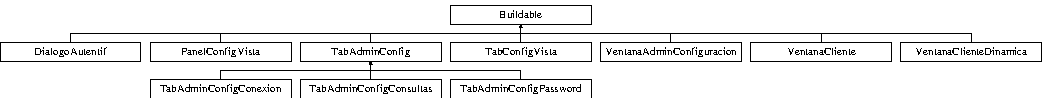
\includegraphics[height=1.318681cm]{classBuildable}
\end{center}
\end{figure}
\subsection*{\-Métodos públicos}
\begin{DoxyCompactItemize}
\item 
\hyperlink{classBuildable_a2d8ab7ff5f0b0875154e2bf8354ea16c}{\-Buildable} (const \-Glib\-::\-Ref\-Ptr$<$ \-Gtk\-::\-Builder $>$ \&\-\_\-builder)
\end{DoxyCompactItemize}
\subsection*{\-Métodos protegidos}
\begin{DoxyCompactItemize}
\item 
{\footnotesize template$<$typename T\-\_\-\-Widget $>$ }\\void \hyperlink{classBuildable_a5a7288ca405c8b322afbea651780e775}{get\-\_\-widget} (const \-Glib\-::ustring \&nombre, \-T\-\_\-\-Widget $\ast$\&p\-Widget)
\item 
{\footnotesize template$<$typename T\-\_\-\-Widget $>$ }\\void \hyperlink{classBuildable_a0de0a59fac2e5ea61786221b31b9b974}{get\-\_\-widget\-\_\-derived} (const \-Glib\-::ustring \&nombre, \-T\-\_\-\-Widget $\ast$\&p\-Widget)
\end{DoxyCompactItemize}
\subsection*{\-Atributos protegidos}
\begin{DoxyCompactItemize}
\item 
\hypertarget{classBuildable_ae7f0098739d2ed693d2f1cf8a8842550}{\-Glib\-::\-Ref\-Ptr$<$ \-Gtk\-::\-Builder $>$ {\bfseries builder}}\label{classBuildable_ae7f0098739d2ed693d2f1cf8a8842550}

\end{DoxyCompactItemize}


\subsection{\-Descripción detallada}
\-Clase \char`\"{}helper\char`\"{} para que todas las que se construyen desde un archivo \-G\-L\-A\-D\-E tengan métodos más limpios. Éstos, además de conseguir la referencia al objeto buscado, verifican la existencia y lanzan la excepción si deben. 

\subsection{\-Documentación del constructor y destructor}
\hypertarget{classBuildable_a2d8ab7ff5f0b0875154e2bf8354ea16c}{\index{\-Buildable@{\-Buildable}!\-Buildable@{\-Buildable}}
\index{\-Buildable@{\-Buildable}!Buildable@{\-Buildable}}
\subsubsection[{\-Buildable}]{\setlength{\rightskip}{0pt plus 5cm}{\bf \-Buildable\-::\-Buildable} (
\begin{DoxyParamCaption}
\item[{const \-Glib\-::\-Ref\-Ptr$<$ \-Gtk\-::\-Builder $>$ \&}]{\-\_\-builder}
\end{DoxyParamCaption}
)\hspace{0.3cm}{\ttfamily  \mbox{[}inline\mbox{]}}}}\label{classBuildable_a2d8ab7ff5f0b0875154e2bf8354ea16c}
\-Constructor, crea la referencia al \-Gtk\-::\-Builder 
\begin{DoxyParams}{\-Parámetros}
{\em \-\_\-builder} & referencia a la instancia que lo construye \\
\hline
\end{DoxyParams}


\subsection{\-Documentación de las funciones miembro}
\hypertarget{classBuildable_a5a7288ca405c8b322afbea651780e775}{\index{\-Buildable@{\-Buildable}!get\-\_\-widget@{get\-\_\-widget}}
\index{get\-\_\-widget@{get\-\_\-widget}!Buildable@{\-Buildable}}
\subsubsection[{get\-\_\-widget}]{\setlength{\rightskip}{0pt plus 5cm}template$<$typename T\-\_\-\-Widget $>$ void {\bf \-Buildable\-::get\-\_\-widget} (
\begin{DoxyParamCaption}
\item[{const \-Glib\-::ustring \&}]{nombre, }
\item[{\-T\-\_\-\-Widget $\ast$\&}]{p\-Widget}
\end{DoxyParamCaption}
)\hspace{0.3cm}{\ttfamily  \mbox{[}inline, protected\mbox{]}}}}\label{classBuildable_a5a7288ca405c8b322afbea651780e775}
wrapper a \-Gtk\-::\-Builder\-::get\-\_\-widget(const \-Glib\-::ustring\& , \-T\-\_\-\-Widget$\ast$\& ) que verifica existencia 
\begin{DoxyParams}{\-Parámetros}
{\em nombre} & nombre del objeto a obtener \\
\hline
\end{DoxyParams}

\begin{DoxyRetVals}{\-Valores devueltos}
{\em p\-Widget} & puntero al objeto buscado \\
\hline
\end{DoxyRetVals}

\begin{DoxyExceptions}{\-Excepciones}
{\em instancia} & de \-Excepcion\-Archivo\-Glade\-Corrupto(nombre) \\
\hline
\end{DoxyExceptions}
\hypertarget{classBuildable_a0de0a59fac2e5ea61786221b31b9b974}{\index{\-Buildable@{\-Buildable}!get\-\_\-widget\-\_\-derived@{get\-\_\-widget\-\_\-derived}}
\index{get\-\_\-widget\-\_\-derived@{get\-\_\-widget\-\_\-derived}!Buildable@{\-Buildable}}
\subsubsection[{get\-\_\-widget\-\_\-derived}]{\setlength{\rightskip}{0pt plus 5cm}template$<$typename T\-\_\-\-Widget $>$ void {\bf \-Buildable\-::get\-\_\-widget\-\_\-derived} (
\begin{DoxyParamCaption}
\item[{const \-Glib\-::ustring \&}]{nombre, }
\item[{\-T\-\_\-\-Widget $\ast$\&}]{p\-Widget}
\end{DoxyParamCaption}
)\hspace{0.3cm}{\ttfamily  \mbox{[}inline, protected\mbox{]}}}}\label{classBuildable_a0de0a59fac2e5ea61786221b31b9b974}
wrapper a \-Gtk\-::\-Builder\-::get\-\_\-widget\-\_\-derived(const \-Glib\-::ustring\& , \-T\-\_\-\-Widget$\ast$\& ) que verifica existencia 
\begin{DoxyParams}{\-Parámetros}
{\em nombre} & nombre del objeto a obtener \\
\hline
\end{DoxyParams}

\begin{DoxyRetVals}{\-Valores devueltos}
{\em p\-Widget} & puntero al objeto buscado \\
\hline
\end{DoxyRetVals}

\begin{DoxyExceptions}{\-Excepciones}
{\em instancia} & de \-Excepcion\-Archivo\-Glade\-Corrupto(nombre) \\
\hline
\end{DoxyExceptions}


\-La documentación para esta clase fue generada a partir del siguiente fichero\-:\begin{DoxyCompactItemize}
\item 
cliente/\-Vista/\-Buildable.\-h\end{DoxyCompactItemize}

\hypertarget{classccsCliente}{\section{\-Referencia de la \-Clase ccs\-Cliente}
\label{classccsCliente}\index{ccs\-Cliente@{ccs\-Cliente}}
}
\-Diagrama de herencias de ccs\-Cliente\begin{figure}[H]
\begin{center}
\leavevmode
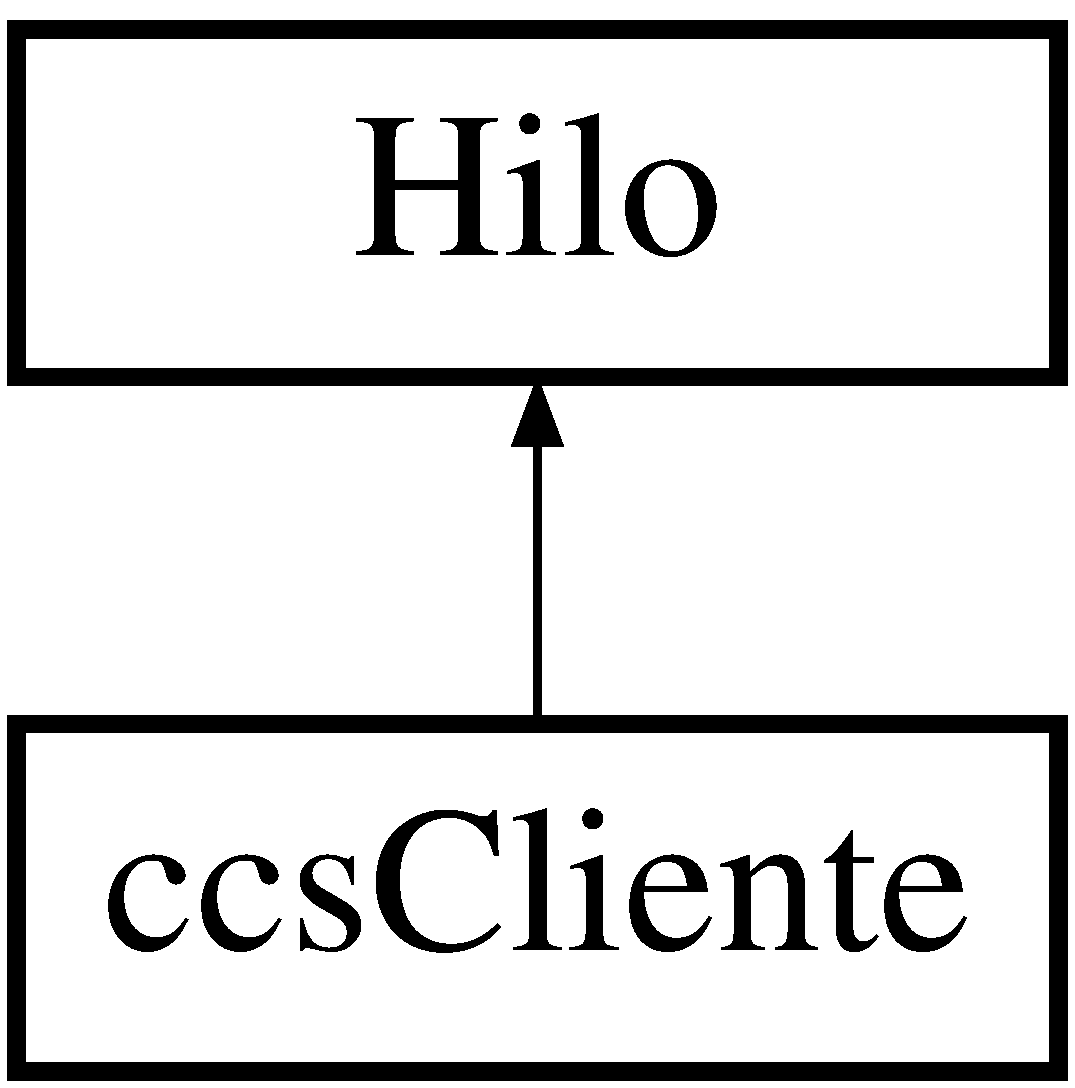
\includegraphics[height=2.000000cm]{classccsCliente}
\end{center}
\end{figure}
\subsection*{\-Métodos públicos}
\begin{DoxyCompactItemize}
\item 
\hypertarget{classccsCliente_aa0797528dcd3b5aa3162c0efe49a890c}{virtual void \hyperlink{classccsCliente_aa0797528dcd3b5aa3162c0efe49a890c}{correr} ()}\label{classccsCliente_aa0797528dcd3b5aa3162c0efe49a890c}

\begin{DoxyCompactList}\small\item\em \-Metodo virtual puro, que corre cuando se ejecuta el hilo. \end{DoxyCompactList}\end{DoxyCompactItemize}
\subsection*{\-Atributos públicos}
\begin{DoxyCompactItemize}
\item 
\hypertarget{classccsCliente_ad830df2e24f6b4d78db9a5dfbaa1adf3}{\hyperlink{classSocket}{\-Socket} {\bfseries \-\_\-sck}}\label{classccsCliente_ad830df2e24f6b4d78db9a5dfbaa1adf3}

\end{DoxyCompactItemize}


\-La documentación para esta clase fue generada a partir del siguiente fichero\-:\begin{DoxyCompactItemize}
\item 
\-Pruebas/\-Prueba\-C\-C\-S.\-h\end{DoxyCompactItemize}

\hypertarget{classccsServidor}{\section{\-Referencia de la \-Clase ccs\-Servidor}
\label{classccsServidor}\index{ccs\-Servidor@{ccs\-Servidor}}
}
\-Diagrama de herencias de ccs\-Servidor\begin{figure}[H]
\begin{center}
\leavevmode
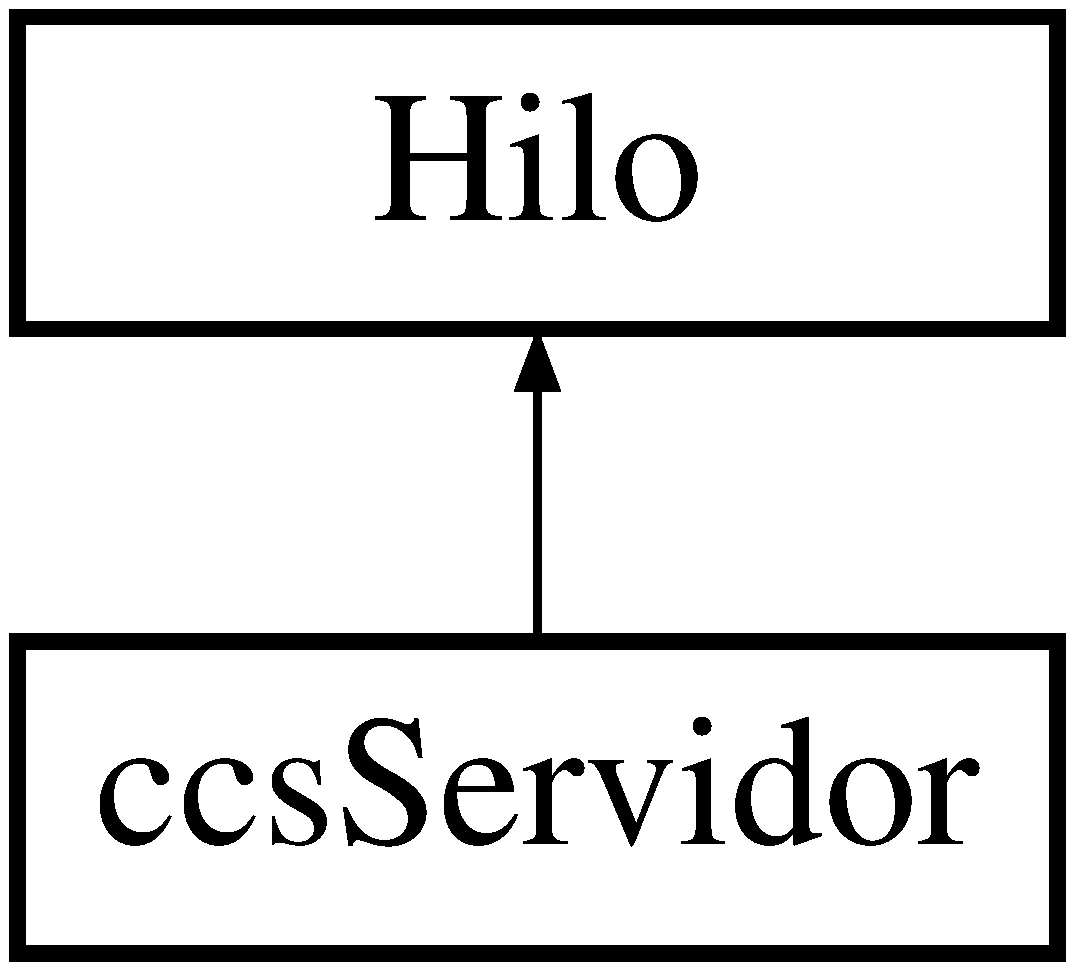
\includegraphics[height=2.000000cm]{classccsServidor}
\end{center}
\end{figure}
\subsection*{\-Métodos públicos}
\begin{DoxyCompactItemize}
\item 
\hypertarget{classccsServidor_adb932252cd6a818744a3017dfbcc0605}{virtual void \hyperlink{classccsServidor_adb932252cd6a818744a3017dfbcc0605}{correr} ()}\label{classccsServidor_adb932252cd6a818744a3017dfbcc0605}

\begin{DoxyCompactList}\small\item\em \-Metodo virtual puro, que corre cuando se ejecuta el hilo. \end{DoxyCompactList}\end{DoxyCompactItemize}


\-La documentación para esta clase fue generada a partir del siguiente fichero\-:\begin{DoxyCompactItemize}
\item 
\-Pruebas/\-Prueba\-C\-C\-S.\-h\end{DoxyCompactItemize}

\hypertarget{classCifrador}{\section{\-Referencia de la \-Clase \-Cifrador}
\label{classCifrador}\index{\-Cifrador@{\-Cifrador}}
}


{\ttfamily \#include $<$\-Cifrador.\-hpp$>$}

\subsection*{\-Métodos públicos}
\begin{DoxyCompactItemize}
\item 
\hypertarget{classCifrador_a539215bcf586cccfc1bcb9f5d3493c4c}{void {\bfseries cifrar} (std\-::string \&obj, int clave=\-D\-E\-F\-A\-U\-L\-T)}\label{classCifrador_a539215bcf586cccfc1bcb9f5d3493c4c}

\item 
\hypertarget{classCifrador_a04cfe0accee25bdfc1dead7cae540b08}{void {\bfseries descifrar} (std\-::string \&obj, int clave=\-D\-E\-F\-A\-U\-L\-T)}\label{classCifrador_a04cfe0accee25bdfc1dead7cae540b08}

\end{DoxyCompactItemize}


\subsection{\-Descripción detallada}
\-Cifra y descifra mensajes. \-Aplica un cifrado básico. 

\-La documentación para esta clase fue generada a partir del siguiente fichero\-:\begin{DoxyCompactItemize}
\item 
comun/\-Cifrador.\-hpp\end{DoxyCompactItemize}

\hypertarget{classCliente}{\section{\-Referencia de la \-Clase \-Cliente}
\label{classCliente}\index{\-Cliente@{\-Cliente}}
}


{\ttfamily \#include $<$\-Cliente.\-h$>$}

\subsection*{\-Métodos públicos}
\begin{DoxyCompactItemize}
\item 
\hyperlink{classCliente_a7d6782c1e479070bdd8c61a6f027ed19}{\-Cliente} (int argc, char $\ast$argv\mbox{[}$\,$\mbox{]})
\item 
\hyperlink{classCliente_a29d1d53394350c66363109e33c990b58}{$\sim$\-Cliente} ()
\item 
\hypertarget{classCliente_a14eb8dac2c8fd77e943fd09640bd38ee}{void {\bfseries run} ()}\label{classCliente_a14eb8dac2c8fd77e943fd09640bd38ee}

\end{DoxyCompactItemize}


\subsection{\-Descripción detallada}
\-Clase que comprende la abstracción de la aplicación en sí, manejando la ventana principal, la carga desde el archivo \-G\-L\-A\-D\-E y de configuración de pestañas, y el main loop de \-G\-T\-K+. 

\subsection{\-Documentación del constructor y destructor}
\hypertarget{classCliente_a7d6782c1e479070bdd8c61a6f027ed19}{\index{\-Cliente@{\-Cliente}!\-Cliente@{\-Cliente}}
\index{\-Cliente@{\-Cliente}!Cliente@{\-Cliente}}
\subsubsection[{\-Cliente}]{\setlength{\rightskip}{0pt plus 5cm}{\bf \-Cliente\-::\-Cliente} (
\begin{DoxyParamCaption}
\item[{int}]{argc, }
\item[{char $\ast$}]{argv\mbox{[}$\,$\mbox{]}}
\end{DoxyParamCaption}
)}}\label{classCliente_a7d6782c1e479070bdd8c61a6f027ed19}
\-Constructor. 
\begin{DoxyParams}{\-Parámetros}
{\em argc} & cantidad de argumentos del programa \\
\hline
{\em argv} & vector de argumentos del programa \\
\hline
\end{DoxyParams}
\hypertarget{classCliente_a29d1d53394350c66363109e33c990b58}{\index{\-Cliente@{\-Cliente}!$\sim$\-Cliente@{$\sim$\-Cliente}}
\index{$\sim$\-Cliente@{$\sim$\-Cliente}!Cliente@{\-Cliente}}
\subsubsection[{$\sim$\-Cliente}]{\setlength{\rightskip}{0pt plus 5cm}{\bf \-Cliente\-::$\sim$\-Cliente} (
\begin{DoxyParamCaption}
{}
\end{DoxyParamCaption}
)}}\label{classCliente_a29d1d53394350c66363109e33c990b58}
\-Destructor. 

\-La documentación para esta clase fue generada a partir de los siguientes ficheros\-:\begin{DoxyCompactItemize}
\item 
cliente/\-Modelo/\-Cliente.\-h\item 
cliente/\-Modelo/\-Cliente.\-cpp\end{DoxyCompactItemize}

\hypertarget{classclienteDummy}{\section{\-Referencia de la \-Clase cliente\-Dummy}
\label{classclienteDummy}\index{cliente\-Dummy@{cliente\-Dummy}}
}
\-Diagrama de herencias de cliente\-Dummy\begin{figure}[H]
\begin{center}
\leavevmode
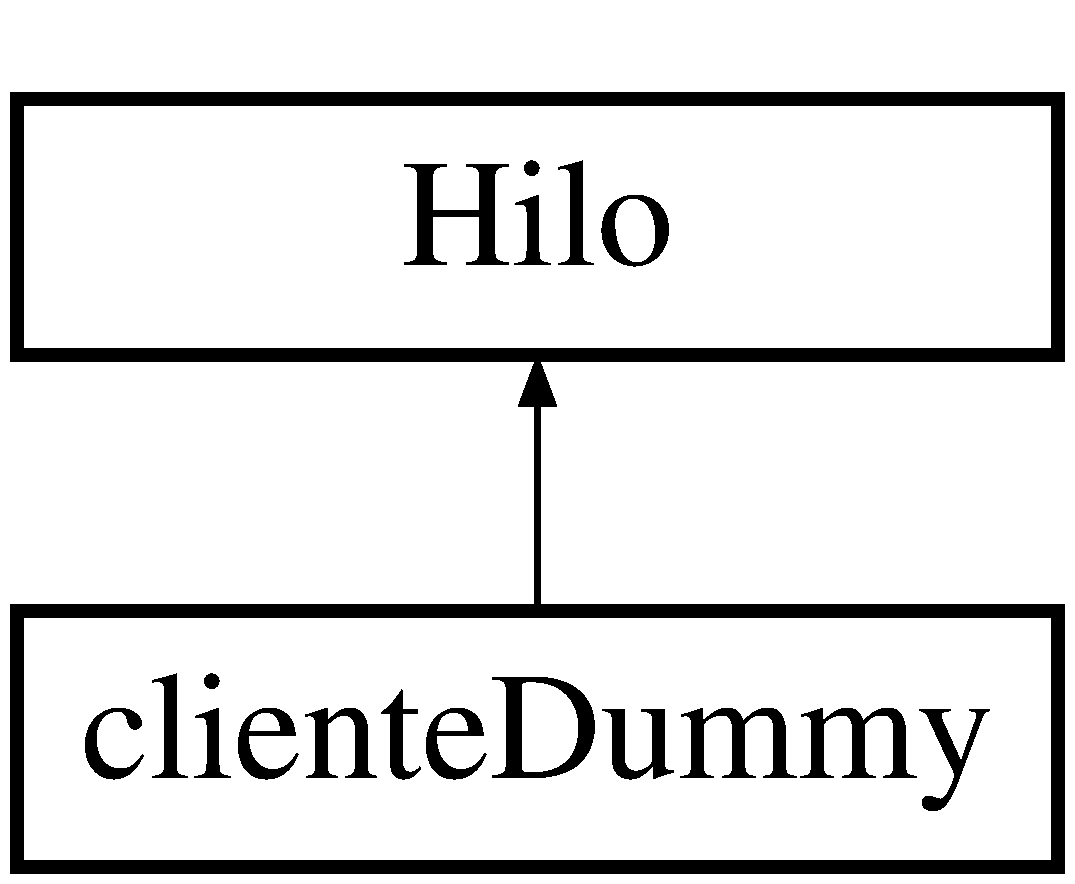
\includegraphics[height=2.000000cm]{classclienteDummy}
\end{center}
\end{figure}
\subsection*{\-Métodos públicos}
\begin{DoxyCompactItemize}
\item 
\hypertarget{classclienteDummy_abb424af4e83e2ec7e4d11d70caa9bcba}{void \hyperlink{classclienteDummy_abb424af4e83e2ec7e4d11d70caa9bcba}{correr} ()}\label{classclienteDummy_abb424af4e83e2ec7e4d11d70caa9bcba}

\begin{DoxyCompactList}\small\item\em \-Metodo virtual puro, que corre cuando se ejecuta el hilo. \end{DoxyCompactList}\end{DoxyCompactItemize}


\-La documentación para esta clase fue generada a partir del siguiente fichero\-:\begin{DoxyCompactItemize}
\item 
servidor/test.\-cpp\end{DoxyCompactItemize}

\hypertarget{classClienteRemoto}{\section{\-Referencia de la \-Clase \-Cliente\-Remoto}
\label{classClienteRemoto}\index{\-Cliente\-Remoto@{\-Cliente\-Remoto}}
}


{\ttfamily \#include $<$\-Cliente\-Remoto.\-h$>$}

\-Diagrama de herencias de \-Cliente\-Remoto\begin{figure}[H]
\begin{center}
\leavevmode
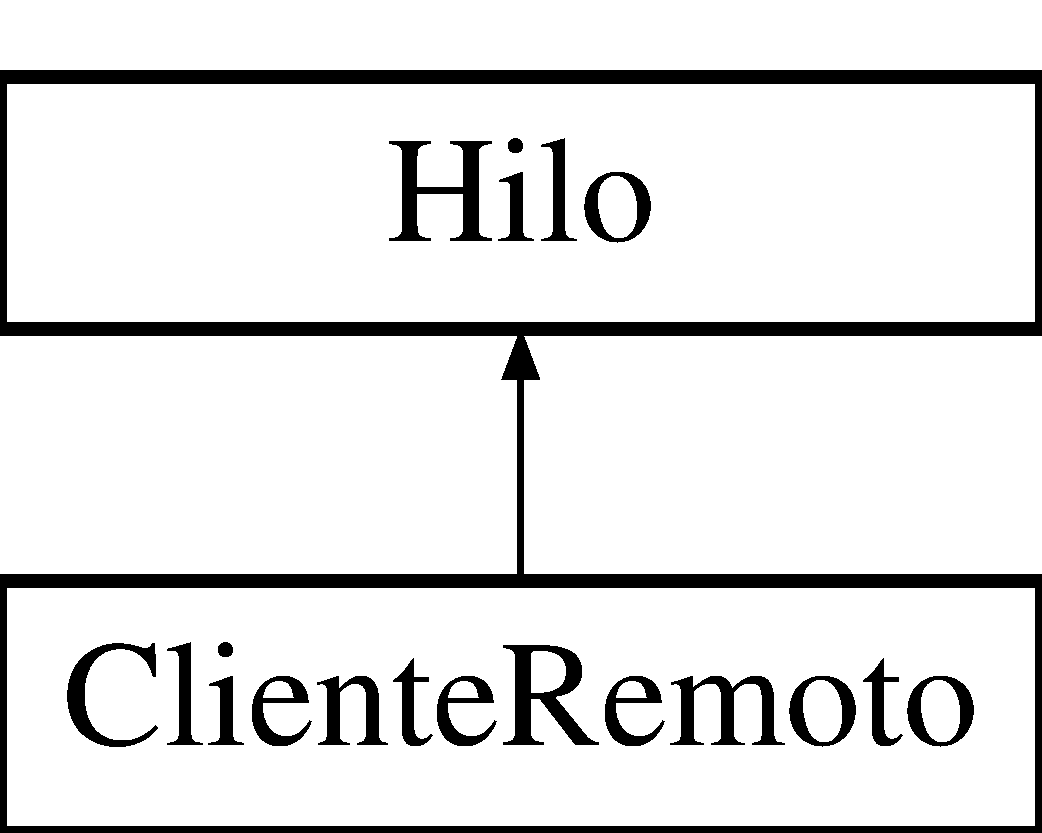
\includegraphics[height=2.000000cm]{classClienteRemoto}
\end{center}
\end{figure}
\subsection*{\-Métodos públicos}
\begin{DoxyCompactItemize}
\item 
void \hyperlink{classClienteRemoto_a741c9308f0d805e09069c79cfad783f4}{correr} ()
\item 
void \hyperlink{classClienteRemoto_af56e06fb4f6e792d9783619b36678df0}{detener\-\_\-cliente} ()
\item 
void \hyperlink{classClienteRemoto_aa73516bc91c7e0967734b11354018bbf}{desconectar\-\_\-cliente} ()
\item 
void \hyperlink{classClienteRemoto_a3364a54ae8e8076743b0867cd4b9375c}{enviar\-Respuesta} (\hyperlink{classRespuesta}{\-Respuesta} \&r)
\item 
\hyperlink{classClienteRemoto_a77480686aca165ca72a7bb316b9918ac}{\-Cliente\-Remoto} (\hyperlink{classSocket}{\-Socket} $\ast$cl, \hyperlink{classResolvedorConsultas}{\-Resolvedor\-Consultas} \&rcons, \hyperlink{classBLQueue}{\-Consultas\-Clientes\-Servidor} \&cons)
\item 
\hyperlink{classClienteRemoto_a14f0c6930666dbbc3b7d4506696f89ef}{$\sim$\-Cliente\-Remoto} ()
\end{DoxyCompactItemize}


\subsection{\-Descripción detallada}
\-Esta clase es el proxy del cliente. \-A través de la misma el servidor obtendrá consultas realizadas y enviará respuestas. \-Es tambien un productor que alimenta la cola de consultas del servidor. \-Se maneja en un hilo aparte, dado que existe un \hyperlink{classClienteRemoto}{\-Cliente\-Remoto} por cliente conectado al servidor. 

\subsection{\-Documentación del constructor y destructor}
\hypertarget{classClienteRemoto_a77480686aca165ca72a7bb316b9918ac}{\index{\-Cliente\-Remoto@{\-Cliente\-Remoto}!\-Cliente\-Remoto@{\-Cliente\-Remoto}}
\index{\-Cliente\-Remoto@{\-Cliente\-Remoto}!ClienteRemoto@{\-Cliente\-Remoto}}
\subsubsection[{\-Cliente\-Remoto}]{\setlength{\rightskip}{0pt plus 5cm}{\bf \-Cliente\-Remoto\-::\-Cliente\-Remoto} (
\begin{DoxyParamCaption}
\item[{{\bf \-Socket} $\ast$}]{cl, }
\item[{{\bf \-Resolvedor\-Consultas} \&}]{rcons, }
\item[{{\bf \-Consultas\-Clientes\-Servidor} \&}]{cons}
\end{DoxyParamCaption}
)}}\label{classClienteRemoto_a77480686aca165ca72a7bb316b9918ac}
constructor del servidor remoto. 
\begin{DoxyParams}{\-Parámetros}
{\em cl} & \hyperlink{classSocket}{\-Socket} activo conectado. \\
\hline
{\em rcons} & \-Objeto encargado de resolver consultas. \\
\hline
{\em cons} & \-Cola de consultas de cliente del servidor. \\
\hline
\end{DoxyParams}
\hypertarget{classClienteRemoto_a14f0c6930666dbbc3b7d4506696f89ef}{\index{\-Cliente\-Remoto@{\-Cliente\-Remoto}!$\sim$\-Cliente\-Remoto@{$\sim$\-Cliente\-Remoto}}
\index{$\sim$\-Cliente\-Remoto@{$\sim$\-Cliente\-Remoto}!ClienteRemoto@{\-Cliente\-Remoto}}
\subsubsection[{$\sim$\-Cliente\-Remoto}]{\setlength{\rightskip}{0pt plus 5cm}{\bf \-Cliente\-Remoto\-::$\sim$\-Cliente\-Remoto} (
\begin{DoxyParamCaption}
{}
\end{DoxyParamCaption}
)}}\label{classClienteRemoto_a14f0c6930666dbbc3b7d4506696f89ef}
\-Destructor de cliente remoto. \-Si esta corriendo, lo detiene. \-Si esta conectado, lo desconecta. 

\subsection{\-Documentación de las funciones miembro}
\hypertarget{classClienteRemoto_a741c9308f0d805e09069c79cfad783f4}{\index{\-Cliente\-Remoto@{\-Cliente\-Remoto}!correr@{correr}}
\index{correr@{correr}!ClienteRemoto@{\-Cliente\-Remoto}}
\subsubsection[{correr}]{\setlength{\rightskip}{0pt plus 5cm}void {\bf \-Cliente\-Remoto\-::correr} (
\begin{DoxyParamCaption}
{}
\end{DoxyParamCaption}
)\hspace{0.3cm}{\ttfamily  \mbox{[}virtual\mbox{]}}}}\label{classClienteRemoto_a741c9308f0d805e09069c79cfad783f4}
\-Método que se ejecuta mientras este en ejecución el hilo. \-Es el encargado de recibir elementos del socket y encolarlos para que responda el servidor. 

\-Implementa \hyperlink{classHilo_a187b055e3504487a6bb64340fac2c70d}{\-Hilo}.

\hypertarget{classClienteRemoto_aa73516bc91c7e0967734b11354018bbf}{\index{\-Cliente\-Remoto@{\-Cliente\-Remoto}!desconectar\-\_\-cliente@{desconectar\-\_\-cliente}}
\index{desconectar\-\_\-cliente@{desconectar\-\_\-cliente}!ClienteRemoto@{\-Cliente\-Remoto}}
\subsubsection[{desconectar\-\_\-cliente}]{\setlength{\rightskip}{0pt plus 5cm}void {\bf \-Cliente\-Remoto\-::desconectar\-\_\-cliente} (
\begin{DoxyParamCaption}
{}
\end{DoxyParamCaption}
)}}\label{classClienteRemoto_aa73516bc91c7e0967734b11354018bbf}
\-Desconecta el socket del cliente. \hypertarget{classClienteRemoto_af56e06fb4f6e792d9783619b36678df0}{\index{\-Cliente\-Remoto@{\-Cliente\-Remoto}!detener\-\_\-cliente@{detener\-\_\-cliente}}
\index{detener\-\_\-cliente@{detener\-\_\-cliente}!ClienteRemoto@{\-Cliente\-Remoto}}
\subsubsection[{detener\-\_\-cliente}]{\setlength{\rightskip}{0pt plus 5cm}void {\bf \-Cliente\-Remoto\-::detener\-\_\-cliente} (
\begin{DoxyParamCaption}
{}
\end{DoxyParamCaption}
)}}\label{classClienteRemoto_af56e06fb4f6e792d9783619b36678df0}
\-Detiene la ejecución del cliente remoto. \hypertarget{classClienteRemoto_a3364a54ae8e8076743b0867cd4b9375c}{\index{\-Cliente\-Remoto@{\-Cliente\-Remoto}!enviar\-Respuesta@{enviar\-Respuesta}}
\index{enviar\-Respuesta@{enviar\-Respuesta}!ClienteRemoto@{\-Cliente\-Remoto}}
\subsubsection[{enviar\-Respuesta}]{\setlength{\rightskip}{0pt plus 5cm}void {\bf \-Cliente\-Remoto\-::enviar\-Respuesta} (
\begin{DoxyParamCaption}
\item[{{\bf \-Respuesta} \&}]{r}
\end{DoxyParamCaption}
)}}\label{classClienteRemoto_a3364a54ae8e8076743b0867cd4b9375c}
\-Envía la respuesta obtenida del servidor al cliente. 

\-La documentación para esta clase fue generada a partir de los siguientes ficheros\-:\begin{DoxyCompactItemize}
\item 
servidor/servidor/\-Cliente\-Remoto.\-h\item 
servidor/servidor/\-Cliente\-Remoto.\-cpp\end{DoxyCompactItemize}

\hypertarget{classTabla_1_1ColumnasModelo}{\section{\-Referencia de la \-Clase \-Tabla\-:\-:\-Columnas\-Modelo}
\label{classTabla_1_1ColumnasModelo}\index{\-Tabla\-::\-Columnas\-Modelo@{\-Tabla\-::\-Columnas\-Modelo}}
}


{\ttfamily \#include $<$\-Tabla.\-h$>$}

\subsection*{\-Métodos públicos}
\begin{DoxyCompactItemize}
\item 
\hypertarget{classTabla_1_1ColumnasModelo_aa13f101bfa970bbc0d5e18d3cc01e4b1}{{\bfseries \-Columnas\-Modelo} (int cantidad\-Columnas)}\label{classTabla_1_1ColumnasModelo_aa13f101bfa970bbc0d5e18d3cc01e4b1}

\end{DoxyCompactItemize}
\subsection*{\-Atributos públicos}
\begin{DoxyCompactItemize}
\item 
\hypertarget{classTabla_1_1ColumnasModelo_a10ec0eb254ecb02598b01625cca9452e}{\-Gtk\-::\-Tree\-Model\-Column\*
$<$ std\-::string $>$ $\ast$ {\bfseries \-\_\-columnas}}\label{classTabla_1_1ColumnasModelo_a10ec0eb254ecb02598b01625cca9452e}

\item 
\hypertarget{classTabla_1_1ColumnasModelo_aec1dd0a62a676ccd175e529287c65296}{int {\bfseries \-\_\-cant\-Col}}\label{classTabla_1_1ColumnasModelo_aec1dd0a62a676ccd175e529287c65296}

\end{DoxyCompactItemize}


\subsection{\-Descripción detallada}
\-Modelo detrás de la \hyperlink{classTabla}{\-Tabla}. 

\-La documentación para esta clase fue generada a partir del siguiente fichero\-:\begin{DoxyCompactItemize}
\item 
cliente/\-Vista/\-Tabla.\-h\end{DoxyCompactItemize}

\hypertarget{classComparadorHechos}{\section{\-Referencia de la \-Clase \-Comparador\-Hechos}
\label{classComparadorHechos}\index{\-Comparador\-Hechos@{\-Comparador\-Hechos}}
}


{\ttfamily \#include $<$\-Comparador\-Hechos.\-h$>$}

\subsection*{\-Métodos públicos}
\begin{DoxyCompactItemize}
\item 
\hyperlink{classComparadorHechos_abbb2f6022e4c02a2dcb377a8bbdcb8f5}{\-Comparador\-Hechos} (bool filtar\-Hechos, const \hyperlink{classConsulta}{\-Consulta} \&consulta)
\begin{DoxyCompactList}\small\item\em \-Constructor que se indica si se tiene que filtrar los hechos y la consulta con las caracterizticas del filtrado. \end{DoxyCompactList}\item 
bool \hyperlink{classComparadorHechos_a605a7418045f710e78291954dab499a2}{registro\-Aceptado} (const std\-::string \&registro)
\begin{DoxyCompactList}\small\item\em \-Retorna un bool indicando si el registro a aceptado filtrado o si se debe descartar. \end{DoxyCompactList}\end{DoxyCompactItemize}


\subsection{\-Descripción detallada}
\-Esta clase es la encargada de decidir si un registro en particular debe o no ser filtrado a partir de filtros de \-Hechos. \-Construyendose a partir un \hyperlink{classConsulta}{\-Consulta} en particular. 

\subsection{\-Documentación del constructor y destructor}
\hypertarget{classComparadorHechos_abbb2f6022e4c02a2dcb377a8bbdcb8f5}{\index{\-Comparador\-Hechos@{\-Comparador\-Hechos}!\-Comparador\-Hechos@{\-Comparador\-Hechos}}
\index{\-Comparador\-Hechos@{\-Comparador\-Hechos}!ComparadorHechos@{\-Comparador\-Hechos}}
\subsubsection[{\-Comparador\-Hechos}]{\setlength{\rightskip}{0pt plus 5cm}{\bf \-Comparador\-Hechos\-::\-Comparador\-Hechos} (
\begin{DoxyParamCaption}
\item[{bool}]{filtar\-Hechos, }
\item[{const {\bf \-Consulta} \&}]{consulta}
\end{DoxyParamCaption}
)}}\label{classComparadorHechos_abbb2f6022e4c02a2dcb377a8bbdcb8f5}


\-Constructor que se indica si se tiene que filtrar los hechos y la consulta con las caracterizticas del filtrado. 


\begin{DoxyParams}{\-Parámetros}
{\em filtar\-Hechos} & booleano indicando si hay filtrados de hechos. \\
\hline
{\em consulta} & es la \hyperlink{classConsulta}{\-Consulta} que contiene los datos por los cual filtrar \\
\hline
\end{DoxyParams}


\subsection{\-Documentación de las funciones miembro}
\hypertarget{classComparadorHechos_a605a7418045f710e78291954dab499a2}{\index{\-Comparador\-Hechos@{\-Comparador\-Hechos}!registro\-Aceptado@{registro\-Aceptado}}
\index{registro\-Aceptado@{registro\-Aceptado}!ComparadorHechos@{\-Comparador\-Hechos}}
\subsubsection[{registro\-Aceptado}]{\setlength{\rightskip}{0pt plus 5cm}bool {\bf \-Comparador\-Hechos\-::registro\-Aceptado} (
\begin{DoxyParamCaption}
\item[{const std\-::string \&}]{registro}
\end{DoxyParamCaption}
)}}\label{classComparadorHechos_a605a7418045f710e78291954dab499a2}


\-Retorna un bool indicando si el registro a aceptado filtrado o si se debe descartar. 

registro string que contiene el registro completo a analizar. \begin{DoxyReturn}{\-Devuelve}
booleano indicando si el registro se debe filtrar o descartar. 
\end{DoxyReturn}


\-La documentación para esta clase fue generada a partir de los siguientes ficheros\-:\begin{DoxyCompactItemize}
\item 
servidor/\-Motor\-De\-Consultas/\-Comparador\-Hechos.\-h\item 
servidor/\-Motor\-De\-Consultas/\-Comparador\-Hechos.\-cpp\end{DoxyCompactItemize}

\hypertarget{classConfigModelo}{\section{\-Referencia de la \-Clase \-Config\-Modelo}
\label{classConfigModelo}\index{\-Config\-Modelo@{\-Config\-Modelo}}
}


{\ttfamily \#include $<$\-Config\-Modelo.\-h$>$}

\-Diagrama de herencias de \-Config\-Modelo\begin{figure}[H]
\begin{center}
\leavevmode
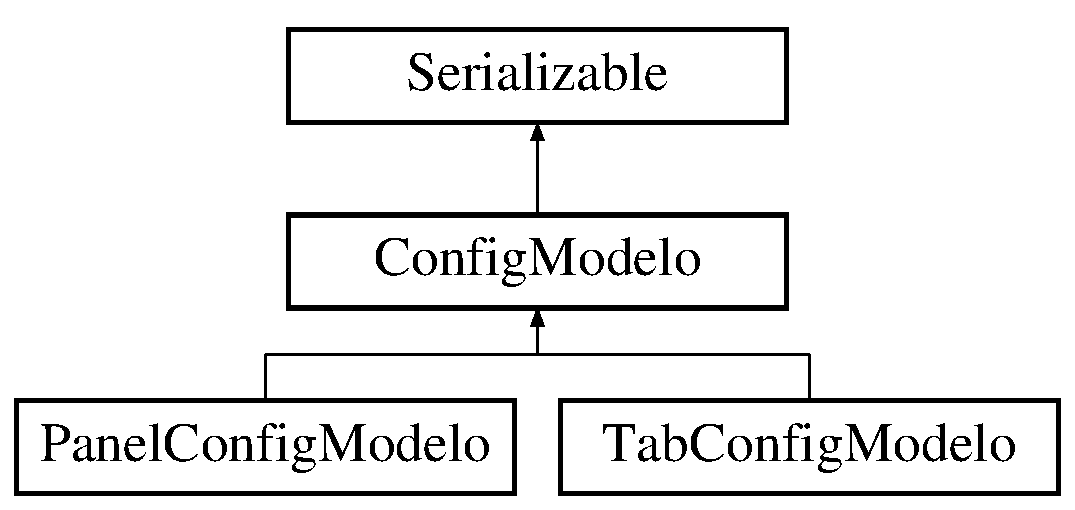
\includegraphics[height=3.000000cm]{classConfigModelo}
\end{center}
\end{figure}
\subsection*{\-Métodos públicos}
\begin{DoxyCompactItemize}
\item 
\hyperlink{classConfigModelo_a128c0b7edc981b8c7f6e5d8f3ee8e9eb}{\-Config\-Modelo} (const \-Glib\-::ustring \&label)
\item 
\hyperlink{classConfigModelo_a5425d7855cf55abe9c8955b92ee9e802}{$\sim$\-Config\-Modelo} ()
\item 
\hypertarget{classConfigModelo_a94d779e447527f246e31f3b65bd28d03}{void {\bfseries desconectar} ()}\label{classConfigModelo_a94d779e447527f246e31f3b65bd28d03}

\item 
\hypertarget{classConfigModelo_a4bed8ed3f91ef9c2bb1064391c2dad8d}{\-Glib\-::ustring {\bfseries get\-Label} () const }\label{classConfigModelo_a4bed8ed3f91ef9c2bb1064391c2dad8d}

\item 
\hypertarget{classConfigModelo_addc4c60afe8773f540c7c672312b5f55}{void {\bfseries set\-Label} (const \-Glib\-::ustring \&label)}\label{classConfigModelo_addc4c60afe8773f540c7c672312b5f55}

\end{DoxyCompactItemize}
\subsection*{\-Métodos protegidos}
\begin{DoxyCompactItemize}
\item 
\hypertarget{classConfigModelo_a40b9aa7742ba791440af155a1055aa24}{{\footnotesize template$<$typename T\-\_\-\-Widget $>$ }\\void {\bfseries desconectar} (sigc\-::connection \&conex, \-T\-\_\-\-Widget $\ast$\&p\-Algo)}\label{classConfigModelo_a40b9aa7742ba791440af155a1055aa24}

\end{DoxyCompactItemize}


\subsection{\-Descripción detallada}
\-Clase base para los modelos que están detrás de las vistas de configuración.

\-Como hay una vista y muchos modelos, tiene la capacidad de desconectarse y reconectarse (cuando le pasan las referencias a la vista).

\-Identificable por su \-Glib\-::ustring label modificable, difieren de los config\-Modelo de los filtradores en eso principalmente. 

\subsection{\-Documentación del constructor y destructor}
\hypertarget{classConfigModelo_a128c0b7edc981b8c7f6e5d8f3ee8e9eb}{\index{\-Config\-Modelo@{\-Config\-Modelo}!\-Config\-Modelo@{\-Config\-Modelo}}
\index{\-Config\-Modelo@{\-Config\-Modelo}!ConfigModelo@{\-Config\-Modelo}}
\subsubsection[{\-Config\-Modelo}]{\setlength{\rightskip}{0pt plus 5cm}{\bf \-Config\-Modelo\-::\-Config\-Modelo} (
\begin{DoxyParamCaption}
\item[{const \-Glib\-::ustring \&}]{label}
\end{DoxyParamCaption}
)}}\label{classConfigModelo_a128c0b7edc981b8c7f6e5d8f3ee8e9eb}
\-Constructor. \hypertarget{classConfigModelo_a5425d7855cf55abe9c8955b92ee9e802}{\index{\-Config\-Modelo@{\-Config\-Modelo}!$\sim$\-Config\-Modelo@{$\sim$\-Config\-Modelo}}
\index{$\sim$\-Config\-Modelo@{$\sim$\-Config\-Modelo}!ConfigModelo@{\-Config\-Modelo}}
\subsubsection[{$\sim$\-Config\-Modelo}]{\setlength{\rightskip}{0pt plus 5cm}{\bf \-Config\-Modelo\-::$\sim$\-Config\-Modelo} (
\begin{DoxyParamCaption}
{}
\end{DoxyParamCaption}
)}}\label{classConfigModelo_a5425d7855cf55abe9c8955b92ee9e802}
\-Destructor. 

\-La documentación para esta clase fue generada a partir de los siguientes ficheros\-:\begin{DoxyCompactItemize}
\item 
cliente/\-Modelo/\-Config\-Modelo.\-h\item 
cliente/\-Modelo/\-Config\-Modelo.\-cpp\end{DoxyCompactItemize}

\hypertarget{classConsulta}{\section{\-Referencia de la \-Clase \-Consulta}
\label{classConsulta}\index{\-Consulta@{\-Consulta}}
}


{\ttfamily \#include $<$\-Consulta.\-h$>$}

\-Diagrama de herencias de \-Consulta\begin{figure}[H]
\begin{center}
\leavevmode
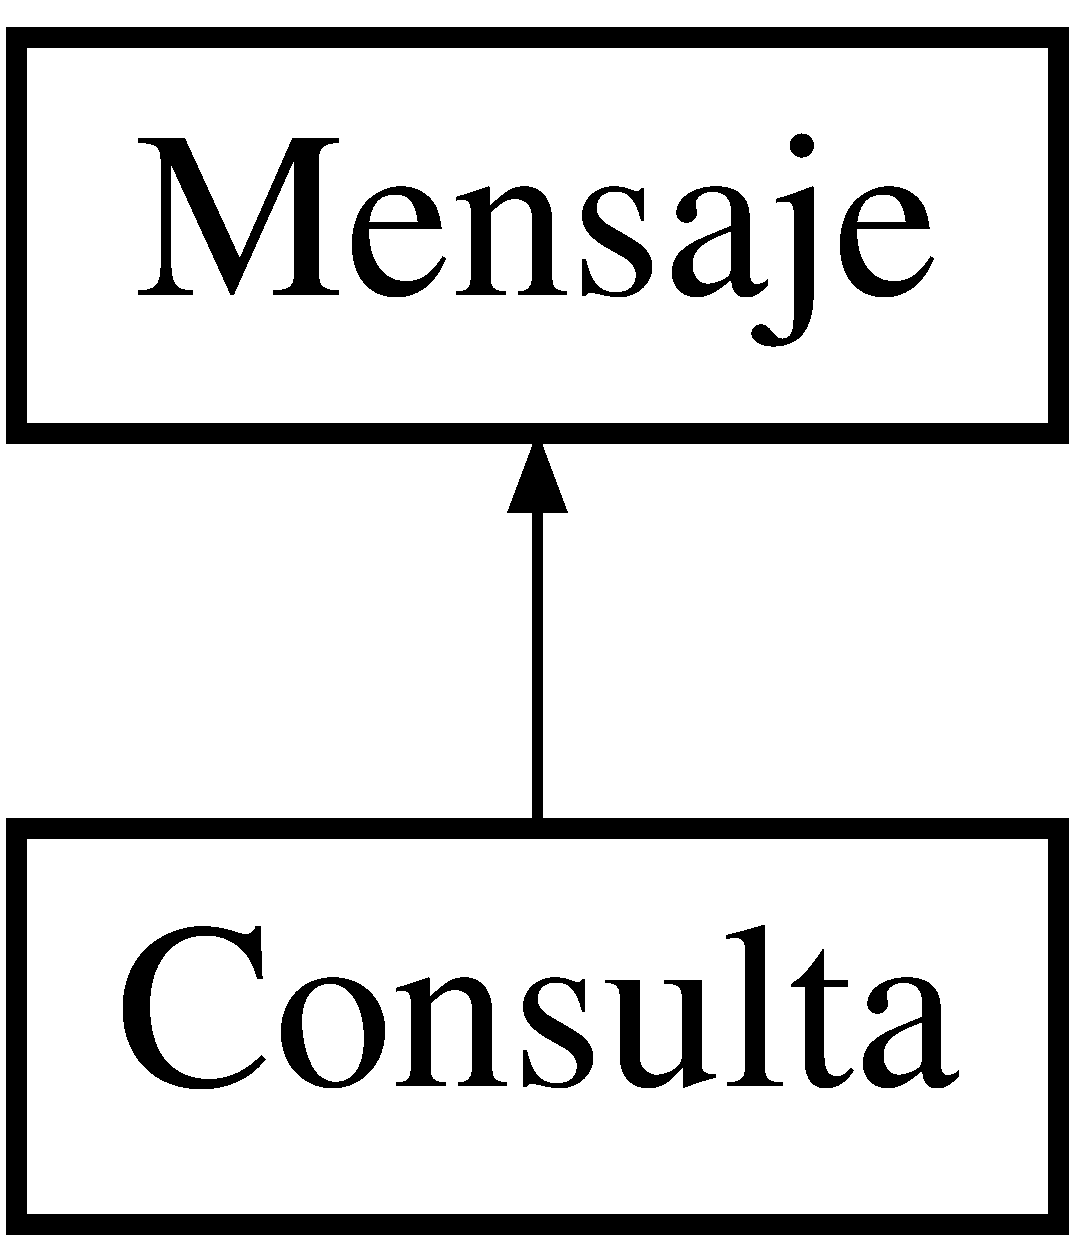
\includegraphics[height=2.000000cm]{classConsulta}
\end{center}
\end{figure}
\subsection*{\-Métodos públicos}
\begin{DoxyCompactItemize}
\item 
\hypertarget{classConsulta_a941db28c9c5f5606fcbfcbd76a4381a7}{\hyperlink{classConsulta_a941db28c9c5f5606fcbfcbd76a4381a7}{\-Consulta} ()}\label{classConsulta_a941db28c9c5f5606fcbfcbd76a4381a7}

\begin{DoxyCompactList}\small\item\em \-Constructor sin argumentos. \end{DoxyCompactList}\item 
\hypertarget{classConsulta_afab55aa5839f10dada36ebe7d6363ca5}{{\bfseries \-Consulta} (const \hyperlink{classConsulta}{\-Consulta} \&original)}\label{classConsulta_afab55aa5839f10dada36ebe7d6363ca5}

\item 
\hyperlink{classConsulta}{\-Consulta} \& \hyperlink{classConsulta_a6acfebe58cc8a740d57ce31276d47fa9}{operator=} (const \hyperlink{classConsulta}{\-Consulta} \&original)
\begin{DoxyCompactList}\small\item\em \-Realiza la copia de otro \hyperlink{classConsulta}{\-Consulta}. \end{DoxyCompactList}\item 
void \hyperlink{classConsulta_a70da0b4ca2b41a62eff57d6f52a67fb8}{definir\-I\-D} (const \-Id\-\_\-\-Mensaje \&id)
\begin{DoxyCompactList}\small\item\em \-Define un nuevo identificador para la \-Consulta(por defecto es 0). \end{DoxyCompactList}\item 
\-Id\-\_\-\-Mensaje \hyperlink{classConsulta_aedb25cbbcb6ee24cc846c29779678bd7}{devolver\-I\-D} () const 
\begin{DoxyCompactList}\small\item\em \-Devuelve el identificador de la \hyperlink{classConsulta}{\-Consulta}. \end{DoxyCompactList}\item 
std\-::string \hyperlink{classConsulta_a0d3fd7d84c1a68b8cbe31a4118150269}{serializar} () const 
\begin{DoxyCompactList}\small\item\em \-Serializa toda la \hyperlink{classConsulta}{\-Consulta} en string. \end{DoxyCompactList}\item 
void \hyperlink{classConsulta_ac3edafd9d21258d9e2b2db753b6a0b61}{deserializar} (const std\-::string \&consulta)
\begin{DoxyCompactList}\small\item\em \-Deserializa la \hyperlink{classConsulta}{\-Consulta} a partir del string. \end{DoxyCompactList}\item 
\hypertarget{classConsulta_a4029f6916b9f06308774422156a14cd3}{void \hyperlink{classConsulta_a4029f6916b9f06308774422156a14cd3}{limpiar} ()}\label{classConsulta_a4029f6916b9f06308774422156a14cd3}

\begin{DoxyCompactList}\small\item\em \-Deja la consulta vacia. \end{DoxyCompactList}\item 
\hypertarget{classConsulta_a9272b3e00577483b722ad30dd398e006}{void \hyperlink{classConsulta_a9272b3e00577483b722ad30dd398e006}{limpiar\-Resultados} ()}\label{classConsulta_a9272b3e00577483b722ad30dd398e006}

\begin{DoxyCompactList}\small\item\em \-Deja la \hyperlink{classConsulta}{\-Consulta} sin \-Resultados pero conservando \-Filtros y \-Entradas. \end{DoxyCompactList}\item 
void \hyperlink{classConsulta_a4df85591716aa2c2ca9f0e305697dcf3}{agregar\-Filtro} (const std\-::string \&\hyperlink{classConsulta_a51966644f6a3fb18e719ba8b10c9f862}{filtro}, const std\-::string \&valor)
\begin{DoxyCompactList}\small\item\em \-Agrega un \-Filtro a la \hyperlink{classConsulta}{\-Consulta}. \end{DoxyCompactList}\item 
void \hyperlink{classConsulta_a78a9d811efd007e8d6d3402123de9494}{agregar\-Entrada} (const std\-::string \hyperlink{classConsulta_a0f8951484349b8b31653615b1ff74bc3}{entrada}, const std\-::string valor)
\begin{DoxyCompactList}\small\item\em \-Agrega una \-Entrada a la \hyperlink{classConsulta}{\-Consulta}. \end{DoxyCompactList}\item 
void \hyperlink{classConsulta_a18c9407b7f8853e18a379ad532e61cd9}{agregar\-Resultado} (const std\-::string \&\hyperlink{classConsulta_acc0fd21c01a4de089670cd5385be4206}{resultado})
\begin{DoxyCompactList}\small\item\em \-Agrega un \-Resultado a la \hyperlink{classConsulta}{\-Consulta}, la agregacion por defecto para el resultado agregado es \char`\"{}\-N\-A\-D\-A\char`\"{}. \end{DoxyCompactList}\item 
void \hyperlink{classConsulta_af9a1f73d3f6120a950cd02068f58893b}{defininir\-Agregacion} (\-Agregacion agregacion, const std\-::string \&\hyperlink{classConsulta_acc0fd21c01a4de089670cd5385be4206}{resultado})
\begin{DoxyCompactList}\small\item\em \-Agrega un \-Resultado a la consulta y define la agregacion del mismo. \end{DoxyCompactList}\item 
\hypertarget{classConsulta_a6020e3a06d8ef8158949ee2d4f6499e0}{void \hyperlink{classConsulta_a6020e3a06d8ef8158949ee2d4f6499e0}{definir\-Como\-Consulta\-Cliente} ()}\label{classConsulta_a6020e3a06d8ef8158949ee2d4f6499e0}

\begin{DoxyCompactList}\small\item\em \-Define el estado de la \hyperlink{classConsulta}{\-Consulta} como consulta de \char`\"{}\-Cliente\char`\"{}. \end{DoxyCompactList}\item 
\hypertarget{classConsulta_a592341b178ed0ab458a4c873dd5492ff}{void \hyperlink{classConsulta_a592341b178ed0ab458a4c873dd5492ff}{definir\-Como\-Consulta\-Agente} ()}\label{classConsulta_a592341b178ed0ab458a4c873dd5492ff}

\begin{DoxyCompactList}\small\item\em \-Define el estado de la \hyperlink{classConsulta}{\-Consulta} como consulta como de \char`\"{}\-Agente\char`\"{}. \end{DoxyCompactList}\item 
\hypertarget{classConsulta_a165215249beb1a7d6da248e234d7d682}{void \hyperlink{classConsulta_a165215249beb1a7d6da248e234d7d682}{definir\-Consulta\-De\-Tabla\-Pivote} ()}\label{classConsulta_a165215249beb1a7d6da248e234d7d682}

\begin{DoxyCompactList}\small\item\em \-Define a la \hyperlink{classConsulta}{\-Consulta} para que la respuesta sea una tabla pivote. \end{DoxyCompactList}\item 
void \hyperlink{classConsulta_aae2c5422470a3471eb7a85938ec6dfe1}{agregar\-X\-Tabla\-P} (const std\-::string \&x)
\begin{DoxyCompactList}\small\item\em agrega un campo al \-Grupo \-X de la \hyperlink{classTabla}{\-Tabla} \-Pivote \end{DoxyCompactList}\item 
void \hyperlink{classConsulta_ab31d73a9ad0c0b3ef5fdc39f8cefe275}{agregar\-Y\-Tabla\-P} (const std\-::string \&y)
\begin{DoxyCompactList}\small\item\em agrega un campo al \-Grupo \-Y de la \hyperlink{classTabla}{\-Tabla} \-Pivote \end{DoxyCompactList}\item 
const std\-::string \& \hyperlink{classConsulta_ab1c28cbebea96855890deaeb156b4777}{x\-De\-Tabla\-Pivote} (unsigned i) const 
\begin{DoxyCompactList}\small\item\em \-Retorna el campo \char`\"{}i\char`\"{} de la \hyperlink{classTabla}{\-Tabla} \-Pivote para el grupo \-X. \end{DoxyCompactList}\item 
const std\-::string \& \hyperlink{classConsulta_a3c42bada58e3474e622dae3951530d82}{y\-De\-Tabla\-Pivote} (unsigned i) const 
\begin{DoxyCompactList}\small\item\em \-Retorna el campo \char`\"{}i\char`\"{} de la \hyperlink{classTabla}{\-Tabla} \-Pivote para el grupo \-Y. \end{DoxyCompactList}\item 
unsigned \hyperlink{classConsulta_a45ef5db7d7d017fb4f3dcded13bee6a2}{cant\-Var\-X\-Tabla} () const 
\begin{DoxyCompactList}\small\item\em \-Indica la cantidad de campos que hay en el \-Grupo \-X de la \hyperlink{classTabla}{\-Tabla} \-Pivote. \end{DoxyCompactList}\item 
unsigned \hyperlink{classConsulta_aeeadf61eb1a51cb8b750950724b3725b}{cant\-Var\-Y\-Tabla} () const 
\begin{DoxyCompactList}\small\item\em \-Indica la cantidad de campos que hay en el \-Grupo \-Y de la \hyperlink{classTabla}{\-Tabla} \-Pivote. \end{DoxyCompactList}\item 
bool \hyperlink{classConsulta_abea0b8acdf1d6dc9dc55998c5a13d022}{es\-Consulta\-De\-Tabla\-Pivote} () const 
\begin{DoxyCompactList}\small\item\em \-Indica si la consulta es de una \hyperlink{classTabla}{\-Tabla} \-Pivote. \end{DoxyCompactList}\item 
void \hyperlink{classConsulta_a353df10eb0afdf7135ffec3ee95d3980}{agregar\-Campo} (const std\-::string \&\hyperlink{classConsulta_a2002e971cfc49f7fdec5f7a9d1de3bf8}{campo})
\begin{DoxyCompactList}\small\item\em \-Agrega un campo a la consulta hecha por el \hyperlink{classAgente}{\-Agente}. \end{DoxyCompactList}\item 
unsigned \hyperlink{classConsulta_a1ebfc9dd876b84c9d97ecf7d60d20aa8}{cantidad\-Filtros} () const 
\begin{DoxyCompactList}\small\item\em \-Retorna la cantidad de filtros que tiene la consulta. \end{DoxyCompactList}\item 
unsigned \hyperlink{classConsulta_a1c1cf418be7d6d4932f5ed4b94900eb8}{cantidad\-Entradas} () const 
\begin{DoxyCompactList}\small\item\em \-Retorna la cantidad de \-Entradas que tiene la consulta. \end{DoxyCompactList}\item 
unsigned \hyperlink{classConsulta_a0b7a5033d52038604faa3c60e1563b6e}{cantidad\-Resultados} () const 
\begin{DoxyCompactList}\small\item\em \-Retorna la cantidad de \-Resultados que posee la consulta. \end{DoxyCompactList}\item 
unsigned \hyperlink{classConsulta_a4bc49d0bdbd55835f463d6d89dee81b6}{cantidad\-Campos} () const 
\begin{DoxyCompactList}\small\item\em \-Retorna la cantidad de campos que tiene la consulta (\-Para que la utilice un a \hyperlink{classAgente}{\-Agente}). \end{DoxyCompactList}\item 
const std\-::string \& \hyperlink{classConsulta_a51966644f6a3fb18e719ba8b10c9f862}{filtro} (unsigned indice) const 
\begin{DoxyCompactList}\small\item\em \-Retorna el \-Filtro indexado por el argumento indice. \end{DoxyCompactList}\item 
const std\-::string \& \hyperlink{classConsulta_a130e8ff49d0f34d4d02124c4b22ff33d}{valor\-Filtro} (unsigned indice) const 
\begin{DoxyCompactList}\small\item\em \-Retorna el valor del \-Filtro indexado por el argumento indice. \end{DoxyCompactList}\item 
const std\-::string \& \hyperlink{classConsulta_a99d8a8e585efeec3757cd46632b01290}{valor\-Filtro} (const std\-::string \&\hyperlink{classConsulta_a51966644f6a3fb18e719ba8b10c9f862}{filtro}) const 
\begin{DoxyCompactList}\small\item\em \-Retorna el valor del \-Filtro indexado por el mismo filtro. \end{DoxyCompactList}\item 
const std\-::string \& \hyperlink{classConsulta_a0f8951484349b8b31653615b1ff74bc3}{entrada} (unsigned indice) const 
\begin{DoxyCompactList}\small\item\em \-Retorna la \-Entrada indexada por el argumento indice. \end{DoxyCompactList}\item 
const std\-::string \& \hyperlink{classConsulta_a0e8eb452c594a166eadc35d3b49a8286}{valor\-Entrada} (unsigned indice) const 
\begin{DoxyCompactList}\small\item\em \-Retorna el \-Valor de la \-Entrada indexada por el argumento indice o por la entrada misma. \end{DoxyCompactList}\item 
const std\-::string \& \hyperlink{classConsulta_a8722053d1fe2d87550c3e1463cee471d}{valor\-Entrada} (const std\-::string \&\hyperlink{classConsulta_a0f8951484349b8b31653615b1ff74bc3}{entrada}) const 
\begin{DoxyCompactList}\small\item\em \-Retorna el \-Valor de la \-Entrada indexada por la misma entrada. \end{DoxyCompactList}\item 
const std\-::string \& \hyperlink{classConsulta_acc0fd21c01a4de089670cd5385be4206}{resultado} (unsigned indice) const 
\begin{DoxyCompactList}\small\item\em \-Retorna el nombre de un resultado indexado por el argumento indice. \end{DoxyCompactList}\item 
\-Agregacion \hyperlink{classConsulta_a51e8e30d03493fd5c818b4ad6bd5fdf3}{agregacion\-De\-Resultado} (unsigned indice) const 
\begin{DoxyCompactList}\small\item\em \-Retorna la agregacion \-Agregacion de \-Resultado. \end{DoxyCompactList}\item 
const std\-::string \& \hyperlink{classConsulta_a2002e971cfc49f7fdec5f7a9d1de3bf8}{campo} (unsigned indice) const 
\begin{DoxyCompactList}\small\item\em \-Retorna un campo de la \char`\"{}\-Consulta\char`\"{} hecha por el agente, indexado por indice. \end{DoxyCompactList}\item 
bool \hyperlink{classConsulta_a721508f359b9391d9b9a906067d9a368}{es\-Consulta\-De\-Cliente} () const 
\begin{DoxyCompactList}\small\item\em \-Indica si la \hyperlink{classConsulta}{\-Consulta} si es una consulta de \hyperlink{classCliente}{\-Cliente}. \end{DoxyCompactList}\item 
bool \hyperlink{classConsulta_a6e39b6d94eba4c3ff0079a7ce64f0008}{es\-Consulta\-De\-Agente} () const 
\begin{DoxyCompactList}\small\item\em \-Indica si es una consulta de \hyperlink{classAgente}{\-Agente}. \end{DoxyCompactList}\end{DoxyCompactItemize}


\subsection{\-Descripción detallada}
\-Esta clase es la encargada de guardar y administrar la consulta realizada por un \hyperlink{classCliente}{\-Cliente} o \hyperlink{classAgente}{\-Agente}, para que sea enviada al servidor y sea resuelta por este. 

\subsection{\-Documentación de las funciones miembro}
\hypertarget{classConsulta_a51e8e30d03493fd5c818b4ad6bd5fdf3}{\index{\-Consulta@{\-Consulta}!agregacion\-De\-Resultado@{agregacion\-De\-Resultado}}
\index{agregacion\-De\-Resultado@{agregacion\-De\-Resultado}!Consulta@{\-Consulta}}
\subsubsection[{agregacion\-De\-Resultado}]{\setlength{\rightskip}{0pt plus 5cm}\-Agregacion {\bf \-Consulta\-::agregacion\-De\-Resultado} (
\begin{DoxyParamCaption}
\item[{unsigned}]{indice}
\end{DoxyParamCaption}
) const}}\label{classConsulta_a51e8e30d03493fd5c818b4ad6bd5fdf3}


\-Retorna la agregacion \-Agregacion de \-Resultado. 


\begin{DoxyParams}{\-Parámetros}
{\em indice} & es el numero del \-Resultado dentro de la consulta. \\
\hline
\end{DoxyParams}
\begin{DoxyReturn}{\-Devuelve}
agregacion del resultado. 
\end{DoxyReturn}
\hypertarget{classConsulta_a353df10eb0afdf7135ffec3ee95d3980}{\index{\-Consulta@{\-Consulta}!agregar\-Campo@{agregar\-Campo}}
\index{agregar\-Campo@{agregar\-Campo}!Consulta@{\-Consulta}}
\subsubsection[{agregar\-Campo}]{\setlength{\rightskip}{0pt plus 5cm}void {\bf \-Consulta\-::agregar\-Campo} (
\begin{DoxyParamCaption}
\item[{const std\-::string \&}]{campo}
\end{DoxyParamCaption}
)}}\label{classConsulta_a353df10eb0afdf7135ffec3ee95d3980}


\-Agrega un campo a la consulta hecha por el \hyperlink{classAgente}{\-Agente}. 


\begin{DoxyParams}{\-Parámetros}
{\em campo} & string que contiene el valor de un campo. \\
\hline
\end{DoxyParams}
\hypertarget{classConsulta_a78a9d811efd007e8d6d3402123de9494}{\index{\-Consulta@{\-Consulta}!agregar\-Entrada@{agregar\-Entrada}}
\index{agregar\-Entrada@{agregar\-Entrada}!Consulta@{\-Consulta}}
\subsubsection[{agregar\-Entrada}]{\setlength{\rightskip}{0pt plus 5cm}void {\bf \-Consulta\-::agregar\-Entrada} (
\begin{DoxyParamCaption}
\item[{const std\-::string}]{entrada, }
\item[{const std\-::string}]{valor}
\end{DoxyParamCaption}
)}}\label{classConsulta_a78a9d811efd007e8d6d3402123de9494}


\-Agrega una \-Entrada a la \hyperlink{classConsulta}{\-Consulta}. 


\begin{DoxyParams}{\-Parámetros}
{\em entrada} & string con el nombre de la entrada \\
\hline
{\em valor} & strinq que contiene el valor de la entrada. \\
\hline
\end{DoxyParams}
\hypertarget{classConsulta_a4df85591716aa2c2ca9f0e305697dcf3}{\index{\-Consulta@{\-Consulta}!agregar\-Filtro@{agregar\-Filtro}}
\index{agregar\-Filtro@{agregar\-Filtro}!Consulta@{\-Consulta}}
\subsubsection[{agregar\-Filtro}]{\setlength{\rightskip}{0pt plus 5cm}void {\bf \-Consulta\-::agregar\-Filtro} (
\begin{DoxyParamCaption}
\item[{const std\-::string \&}]{filtro, }
\item[{const std\-::string \&}]{valor}
\end{DoxyParamCaption}
)}}\label{classConsulta_a4df85591716aa2c2ca9f0e305697dcf3}


\-Agrega un \-Filtro a la \hyperlink{classConsulta}{\-Consulta}. 


\begin{DoxyParams}{\-Parámetros}
{\em filtro} & string con el nombre del filtro \\
\hline
{\em valor} & string que contiene el valor del filtro \\
\hline
\end{DoxyParams}
\hypertarget{classConsulta_a18c9407b7f8853e18a379ad532e61cd9}{\index{\-Consulta@{\-Consulta}!agregar\-Resultado@{agregar\-Resultado}}
\index{agregar\-Resultado@{agregar\-Resultado}!Consulta@{\-Consulta}}
\subsubsection[{agregar\-Resultado}]{\setlength{\rightskip}{0pt plus 5cm}void {\bf \-Consulta\-::agregar\-Resultado} (
\begin{DoxyParamCaption}
\item[{const std\-::string \&}]{resultado}
\end{DoxyParamCaption}
)}}\label{classConsulta_a18c9407b7f8853e18a379ad532e61cd9}


\-Agrega un \-Resultado a la \hyperlink{classConsulta}{\-Consulta}, la agregacion por defecto para el resultado agregado es \char`\"{}\-N\-A\-D\-A\char`\"{}. 


\begin{DoxyParams}{\-Parámetros}
{\em resultado} & string que contiene el nombre del campo a agregar. \\
\hline
\end{DoxyParams}
\hypertarget{classConsulta_aae2c5422470a3471eb7a85938ec6dfe1}{\index{\-Consulta@{\-Consulta}!agregar\-X\-Tabla\-P@{agregar\-X\-Tabla\-P}}
\index{agregar\-X\-Tabla\-P@{agregar\-X\-Tabla\-P}!Consulta@{\-Consulta}}
\subsubsection[{agregar\-X\-Tabla\-P}]{\setlength{\rightskip}{0pt plus 5cm}void {\bf \-Consulta\-::agregar\-X\-Tabla\-P} (
\begin{DoxyParamCaption}
\item[{const std\-::string \&}]{x}
\end{DoxyParamCaption}
)}}\label{classConsulta_aae2c5422470a3471eb7a85938ec6dfe1}


agrega un campo al \-Grupo \-X de la \hyperlink{classTabla}{\-Tabla} \-Pivote 


\begin{DoxyParams}{\-Parámetros}
{\em x} & string con el nombre del campo a agregar. \\
\hline
\end{DoxyParams}
\hypertarget{classConsulta_ab31d73a9ad0c0b3ef5fdc39f8cefe275}{\index{\-Consulta@{\-Consulta}!agregar\-Y\-Tabla\-P@{agregar\-Y\-Tabla\-P}}
\index{agregar\-Y\-Tabla\-P@{agregar\-Y\-Tabla\-P}!Consulta@{\-Consulta}}
\subsubsection[{agregar\-Y\-Tabla\-P}]{\setlength{\rightskip}{0pt plus 5cm}void {\bf \-Consulta\-::agregar\-Y\-Tabla\-P} (
\begin{DoxyParamCaption}
\item[{const std\-::string \&}]{y}
\end{DoxyParamCaption}
)}}\label{classConsulta_ab31d73a9ad0c0b3ef5fdc39f8cefe275}


agrega un campo al \-Grupo \-Y de la \hyperlink{classTabla}{\-Tabla} \-Pivote 


\begin{DoxyParams}{\-Parámetros}
{\em y} & string con el nombre del campo a agregar. \\
\hline
\end{DoxyParams}
\hypertarget{classConsulta_a2002e971cfc49f7fdec5f7a9d1de3bf8}{\index{\-Consulta@{\-Consulta}!campo@{campo}}
\index{campo@{campo}!Consulta@{\-Consulta}}
\subsubsection[{campo}]{\setlength{\rightskip}{0pt plus 5cm}const std\-::string \& {\bf \-Consulta\-::campo} (
\begin{DoxyParamCaption}
\item[{unsigned}]{indice}
\end{DoxyParamCaption}
) const}}\label{classConsulta_a2002e971cfc49f7fdec5f7a9d1de3bf8}


\-Retorna un campo de la \char`\"{}\-Consulta\char`\"{} hecha por el agente, indexado por indice. 


\begin{DoxyParams}{\-Parámetros}
{\em indice} & es el numero del campo dentro de la \hyperlink{classConsulta}{\-Consulta}. \\
\hline
\end{DoxyParams}
\begin{DoxyReturn}{\-Devuelve}
string que contiene el nombre del \-Campo \-Recuperado. 
\end{DoxyReturn}
\hypertarget{classConsulta_a4bc49d0bdbd55835f463d6d89dee81b6}{\index{\-Consulta@{\-Consulta}!cantidad\-Campos@{cantidad\-Campos}}
\index{cantidad\-Campos@{cantidad\-Campos}!Consulta@{\-Consulta}}
\subsubsection[{cantidad\-Campos}]{\setlength{\rightskip}{0pt plus 5cm}unsigned {\bf \-Consulta\-::cantidad\-Campos} (
\begin{DoxyParamCaption}
{}
\end{DoxyParamCaption}
) const}}\label{classConsulta_a4bc49d0bdbd55835f463d6d89dee81b6}


\-Retorna la cantidad de campos que tiene la consulta (\-Para que la utilice un a \hyperlink{classAgente}{\-Agente}). 

\begin{DoxyReturn}{\-Devuelve}
cantidad de campos. 
\end{DoxyReturn}
\hypertarget{classConsulta_a1c1cf418be7d6d4932f5ed4b94900eb8}{\index{\-Consulta@{\-Consulta}!cantidad\-Entradas@{cantidad\-Entradas}}
\index{cantidad\-Entradas@{cantidad\-Entradas}!Consulta@{\-Consulta}}
\subsubsection[{cantidad\-Entradas}]{\setlength{\rightskip}{0pt plus 5cm}unsigned {\bf \-Consulta\-::cantidad\-Entradas} (
\begin{DoxyParamCaption}
{}
\end{DoxyParamCaption}
) const}}\label{classConsulta_a1c1cf418be7d6d4932f5ed4b94900eb8}


\-Retorna la cantidad de \-Entradas que tiene la consulta. 

\begin{DoxyReturn}{\-Devuelve}
cantidad de \-Entradas. 
\end{DoxyReturn}
\hypertarget{classConsulta_a1ebfc9dd876b84c9d97ecf7d60d20aa8}{\index{\-Consulta@{\-Consulta}!cantidad\-Filtros@{cantidad\-Filtros}}
\index{cantidad\-Filtros@{cantidad\-Filtros}!Consulta@{\-Consulta}}
\subsubsection[{cantidad\-Filtros}]{\setlength{\rightskip}{0pt plus 5cm}unsigned {\bf \-Consulta\-::cantidad\-Filtros} (
\begin{DoxyParamCaption}
{}
\end{DoxyParamCaption}
) const}}\label{classConsulta_a1ebfc9dd876b84c9d97ecf7d60d20aa8}


\-Retorna la cantidad de filtros que tiene la consulta. 

\begin{DoxyReturn}{\-Devuelve}
cantidad de \-Filtros. 
\end{DoxyReturn}
\hypertarget{classConsulta_a0b7a5033d52038604faa3c60e1563b6e}{\index{\-Consulta@{\-Consulta}!cantidad\-Resultados@{cantidad\-Resultados}}
\index{cantidad\-Resultados@{cantidad\-Resultados}!Consulta@{\-Consulta}}
\subsubsection[{cantidad\-Resultados}]{\setlength{\rightskip}{0pt plus 5cm}unsigned {\bf \-Consulta\-::cantidad\-Resultados} (
\begin{DoxyParamCaption}
{}
\end{DoxyParamCaption}
) const}}\label{classConsulta_a0b7a5033d52038604faa3c60e1563b6e}


\-Retorna la cantidad de \-Resultados que posee la consulta. 

\begin{DoxyReturn}{\-Devuelve}
cantidad de \-Resultados. 
\end{DoxyReturn}
\hypertarget{classConsulta_a45ef5db7d7d017fb4f3dcded13bee6a2}{\index{\-Consulta@{\-Consulta}!cant\-Var\-X\-Tabla@{cant\-Var\-X\-Tabla}}
\index{cant\-Var\-X\-Tabla@{cant\-Var\-X\-Tabla}!Consulta@{\-Consulta}}
\subsubsection[{cant\-Var\-X\-Tabla}]{\setlength{\rightskip}{0pt plus 5cm}unsigned {\bf \-Consulta\-::cant\-Var\-X\-Tabla} (
\begin{DoxyParamCaption}
{}
\end{DoxyParamCaption}
) const}}\label{classConsulta_a45ef5db7d7d017fb4f3dcded13bee6a2}


\-Indica la cantidad de campos que hay en el \-Grupo \-X de la \hyperlink{classTabla}{\-Tabla} \-Pivote. 

\begin{DoxyReturn}{\-Devuelve}
cantidad de \-Campos 
\end{DoxyReturn}
\hypertarget{classConsulta_aeeadf61eb1a51cb8b750950724b3725b}{\index{\-Consulta@{\-Consulta}!cant\-Var\-Y\-Tabla@{cant\-Var\-Y\-Tabla}}
\index{cant\-Var\-Y\-Tabla@{cant\-Var\-Y\-Tabla}!Consulta@{\-Consulta}}
\subsubsection[{cant\-Var\-Y\-Tabla}]{\setlength{\rightskip}{0pt plus 5cm}unsigned {\bf \-Consulta\-::cant\-Var\-Y\-Tabla} (
\begin{DoxyParamCaption}
{}
\end{DoxyParamCaption}
) const}}\label{classConsulta_aeeadf61eb1a51cb8b750950724b3725b}


\-Indica la cantidad de campos que hay en el \-Grupo \-Y de la \hyperlink{classTabla}{\-Tabla} \-Pivote. 

\begin{DoxyReturn}{\-Devuelve}
cantidad de \-Campos. 
\end{DoxyReturn}
\hypertarget{classConsulta_af9a1f73d3f6120a950cd02068f58893b}{\index{\-Consulta@{\-Consulta}!defininir\-Agregacion@{defininir\-Agregacion}}
\index{defininir\-Agregacion@{defininir\-Agregacion}!Consulta@{\-Consulta}}
\subsubsection[{defininir\-Agregacion}]{\setlength{\rightskip}{0pt plus 5cm}void {\bf \-Consulta\-::defininir\-Agregacion} (
\begin{DoxyParamCaption}
\item[{\-Agregacion}]{agregacion, }
\item[{const std\-::string \&}]{resultado}
\end{DoxyParamCaption}
)}}\label{classConsulta_af9a1f73d3f6120a950cd02068f58893b}


\-Agrega un \-Resultado a la consulta y define la agregacion del mismo. 


\begin{DoxyParams}{\-Parámetros}
{\em agregacion} & tipo de agregacion para el resultado \\
\hline
{\em resultado} & string que contiene el nombre del campo resultado. \\
\hline
\end{DoxyParams}
\hypertarget{classConsulta_a70da0b4ca2b41a62eff57d6f52a67fb8}{\index{\-Consulta@{\-Consulta}!definir\-I\-D@{definir\-I\-D}}
\index{definir\-I\-D@{definir\-I\-D}!Consulta@{\-Consulta}}
\subsubsection[{definir\-I\-D}]{\setlength{\rightskip}{0pt plus 5cm}void {\bf \-Consulta\-::definir\-I\-D} (
\begin{DoxyParamCaption}
\item[{const \-Id\-\_\-\-Mensaje \&}]{id}
\end{DoxyParamCaption}
)}}\label{classConsulta_a70da0b4ca2b41a62eff57d6f52a67fb8}


\-Define un nuevo identificador para la \-Consulta(por defecto es 0). 


\begin{DoxyParams}{\-Parámetros}
{\em id} & nuevo identificador. \\
\hline
\end{DoxyParams}
\hypertarget{classConsulta_ac3edafd9d21258d9e2b2db753b6a0b61}{\index{\-Consulta@{\-Consulta}!deserializar@{deserializar}}
\index{deserializar@{deserializar}!Consulta@{\-Consulta}}
\subsubsection[{deserializar}]{\setlength{\rightskip}{0pt plus 5cm}void {\bf \-Consulta\-::deserializar} (
\begin{DoxyParamCaption}
\item[{const std\-::string \&}]{consulta}
\end{DoxyParamCaption}
)\hspace{0.3cm}{\ttfamily  \mbox{[}virtual\mbox{]}}}}\label{classConsulta_ac3edafd9d21258d9e2b2db753b6a0b61}


\-Deserializa la \hyperlink{classConsulta}{\-Consulta} a partir del string. 


\begin{DoxyParams}{\-Parámetros}
{\em consulta} & string con que contiene la consulta serializada \\
\hline
\end{DoxyParams}


\-Implementa \hyperlink{classMensaje_a49422c2abf7fe32e887ee854cdf6cf25}{\-Mensaje}.

\hypertarget{classConsulta_aedb25cbbcb6ee24cc846c29779678bd7}{\index{\-Consulta@{\-Consulta}!devolver\-I\-D@{devolver\-I\-D}}
\index{devolver\-I\-D@{devolver\-I\-D}!Consulta@{\-Consulta}}
\subsubsection[{devolver\-I\-D}]{\setlength{\rightskip}{0pt plus 5cm}\-Id\-\_\-\-Mensaje {\bf \-Consulta\-::devolver\-I\-D} (
\begin{DoxyParamCaption}
{}
\end{DoxyParamCaption}
) const}}\label{classConsulta_aedb25cbbcb6ee24cc846c29779678bd7}


\-Devuelve el identificador de la \hyperlink{classConsulta}{\-Consulta}. 

\begin{DoxyReturn}{\-Devuelve}
id de la \hyperlink{classConsulta}{\-Consulta}. 
\end{DoxyReturn}
\hypertarget{classConsulta_a0f8951484349b8b31653615b1ff74bc3}{\index{\-Consulta@{\-Consulta}!entrada@{entrada}}
\index{entrada@{entrada}!Consulta@{\-Consulta}}
\subsubsection[{entrada}]{\setlength{\rightskip}{0pt plus 5cm}const std\-::string \& {\bf \-Consulta\-::entrada} (
\begin{DoxyParamCaption}
\item[{unsigned}]{indice}
\end{DoxyParamCaption}
) const}}\label{classConsulta_a0f8951484349b8b31653615b1ff74bc3}


\-Retorna la \-Entrada indexada por el argumento indice. 


\begin{DoxyParams}{\-Parámetros}
{\em indice} & es el indice de la \-Entrada dentro de la \hyperlink{classConsulta}{\-Consulta}. \\
\hline
\end{DoxyParams}
\begin{DoxyReturn}{\-Devuelve}
string que contiene el nombre de la \-Entrada. 
\end{DoxyReturn}
\hypertarget{classConsulta_a6e39b6d94eba4c3ff0079a7ce64f0008}{\index{\-Consulta@{\-Consulta}!es\-Consulta\-De\-Agente@{es\-Consulta\-De\-Agente}}
\index{es\-Consulta\-De\-Agente@{es\-Consulta\-De\-Agente}!Consulta@{\-Consulta}}
\subsubsection[{es\-Consulta\-De\-Agente}]{\setlength{\rightskip}{0pt plus 5cm}bool {\bf \-Consulta\-::es\-Consulta\-De\-Agente} (
\begin{DoxyParamCaption}
{}
\end{DoxyParamCaption}
) const}}\label{classConsulta_a6e39b6d94eba4c3ff0079a7ce64f0008}


\-Indica si es una consulta de \hyperlink{classAgente}{\-Agente}. 

\begin{DoxyReturn}{\-Devuelve}
booleano que indica si una consulta de \hyperlink{classAgente}{\-Agente}. 
\end{DoxyReturn}
\hypertarget{classConsulta_a721508f359b9391d9b9a906067d9a368}{\index{\-Consulta@{\-Consulta}!es\-Consulta\-De\-Cliente@{es\-Consulta\-De\-Cliente}}
\index{es\-Consulta\-De\-Cliente@{es\-Consulta\-De\-Cliente}!Consulta@{\-Consulta}}
\subsubsection[{es\-Consulta\-De\-Cliente}]{\setlength{\rightskip}{0pt plus 5cm}bool {\bf \-Consulta\-::es\-Consulta\-De\-Cliente} (
\begin{DoxyParamCaption}
{}
\end{DoxyParamCaption}
) const}}\label{classConsulta_a721508f359b9391d9b9a906067d9a368}


\-Indica si la \hyperlink{classConsulta}{\-Consulta} si es una consulta de \hyperlink{classCliente}{\-Cliente}. 

\begin{DoxyReturn}{\-Devuelve}
booleano que indica si una consulta de \hyperlink{classCliente}{\-Cliente}. 
\end{DoxyReturn}
\hypertarget{classConsulta_abea0b8acdf1d6dc9dc55998c5a13d022}{\index{\-Consulta@{\-Consulta}!es\-Consulta\-De\-Tabla\-Pivote@{es\-Consulta\-De\-Tabla\-Pivote}}
\index{es\-Consulta\-De\-Tabla\-Pivote@{es\-Consulta\-De\-Tabla\-Pivote}!Consulta@{\-Consulta}}
\subsubsection[{es\-Consulta\-De\-Tabla\-Pivote}]{\setlength{\rightskip}{0pt plus 5cm}bool {\bf \-Consulta\-::es\-Consulta\-De\-Tabla\-Pivote} (
\begin{DoxyParamCaption}
{}
\end{DoxyParamCaption}
) const}}\label{classConsulta_abea0b8acdf1d6dc9dc55998c5a13d022}


\-Indica si la consulta es de una \hyperlink{classTabla}{\-Tabla} \-Pivote. 

\begin{DoxyReturn}{\-Devuelve}
booleano que indica si consulta de \hyperlink{classTabla}{\-Tabla} \-Pivote 
\end{DoxyReturn}
\hypertarget{classConsulta_a51966644f6a3fb18e719ba8b10c9f862}{\index{\-Consulta@{\-Consulta}!filtro@{filtro}}
\index{filtro@{filtro}!Consulta@{\-Consulta}}
\subsubsection[{filtro}]{\setlength{\rightskip}{0pt plus 5cm}const std\-::string \& {\bf \-Consulta\-::filtro} (
\begin{DoxyParamCaption}
\item[{unsigned}]{indice}
\end{DoxyParamCaption}
) const}}\label{classConsulta_a51966644f6a3fb18e719ba8b10c9f862}


\-Retorna el \-Filtro indexado por el argumento indice. 


\begin{DoxyParams}{\-Parámetros}
{\em indice} & es el indice del \-Filtro dentro de la \hyperlink{classConsulta}{\-Consulta} \\
\hline
\end{DoxyParams}
\begin{DoxyReturn}{\-Devuelve}
nombre del \-Filtro recuperado. 
\end{DoxyReturn}
\hypertarget{classConsulta_a6acfebe58cc8a740d57ce31276d47fa9}{\index{\-Consulta@{\-Consulta}!operator=@{operator=}}
\index{operator=@{operator=}!Consulta@{\-Consulta}}
\subsubsection[{operator=}]{\setlength{\rightskip}{0pt plus 5cm}{\bf \-Consulta} \& \-Consulta\-::operator= (
\begin{DoxyParamCaption}
\item[{const {\bf \-Consulta} \&}]{original}
\end{DoxyParamCaption}
)}}\label{classConsulta_a6acfebe58cc8a740d57ce31276d47fa9}


\-Realiza la copia de otro \hyperlink{classConsulta}{\-Consulta}. 


\begin{DoxyParams}{\-Parámetros}
{\em original} & consulta a copiar. \\
\hline
\end{DoxyParams}
\begin{DoxyReturn}{\-Devuelve}
referecia de la \hyperlink{classConsulta}{\-Consulta} actual. 
\end{DoxyReturn}
\hypertarget{classConsulta_acc0fd21c01a4de089670cd5385be4206}{\index{\-Consulta@{\-Consulta}!resultado@{resultado}}
\index{resultado@{resultado}!Consulta@{\-Consulta}}
\subsubsection[{resultado}]{\setlength{\rightskip}{0pt plus 5cm}const std\-::string \& {\bf \-Consulta\-::resultado} (
\begin{DoxyParamCaption}
\item[{unsigned}]{indice}
\end{DoxyParamCaption}
) const}}\label{classConsulta_acc0fd21c01a4de089670cd5385be4206}


\-Retorna el nombre de un resultado indexado por el argumento indice. 


\begin{DoxyParams}{\-Parámetros}
{\em indice} & es el numero del \-Resultado dentro de la consulta. \\
\hline
\end{DoxyParams}
\begin{DoxyReturn}{\-Devuelve}
string que contiene el nombre del \-Resultado recuperado. 
\end{DoxyReturn}
\hypertarget{classConsulta_a0d3fd7d84c1a68b8cbe31a4118150269}{\index{\-Consulta@{\-Consulta}!serializar@{serializar}}
\index{serializar@{serializar}!Consulta@{\-Consulta}}
\subsubsection[{serializar}]{\setlength{\rightskip}{0pt plus 5cm}std\-::string {\bf \-Consulta\-::serializar} (
\begin{DoxyParamCaption}
{}
\end{DoxyParamCaption}
) const\hspace{0.3cm}{\ttfamily  \mbox{[}virtual\mbox{]}}}}\label{classConsulta_a0d3fd7d84c1a68b8cbe31a4118150269}


\-Serializa toda la \hyperlink{classConsulta}{\-Consulta} en string. 

\begin{DoxyReturn}{\-Devuelve}
string que contiene la \hyperlink{classConsulta}{\-Consulta} serializada. 
\end{DoxyReturn}


\-Implementa \hyperlink{classMensaje_afd69cd129ca7ce1cf967a6f3690ad904}{\-Mensaje}.

\hypertarget{classConsulta_a0e8eb452c594a166eadc35d3b49a8286}{\index{\-Consulta@{\-Consulta}!valor\-Entrada@{valor\-Entrada}}
\index{valor\-Entrada@{valor\-Entrada}!Consulta@{\-Consulta}}
\subsubsection[{valor\-Entrada}]{\setlength{\rightskip}{0pt plus 5cm}const std\-::string \& {\bf \-Consulta\-::valor\-Entrada} (
\begin{DoxyParamCaption}
\item[{unsigned}]{indice}
\end{DoxyParamCaption}
) const}}\label{classConsulta_a0e8eb452c594a166eadc35d3b49a8286}


\-Retorna el \-Valor de la \-Entrada indexada por el argumento indice o por la entrada misma. 


\begin{DoxyParams}{\-Parámetros}
{\em indice} & es el indice de la \-Entrada dentro de la \hyperlink{classConsulta}{\-Consulta} \\
\hline
\end{DoxyParams}
\begin{DoxyReturn}{\-Devuelve}
string que contiene el valor de la \-Entrada. 
\end{DoxyReturn}
\hypertarget{classConsulta_a8722053d1fe2d87550c3e1463cee471d}{\index{\-Consulta@{\-Consulta}!valor\-Entrada@{valor\-Entrada}}
\index{valor\-Entrada@{valor\-Entrada}!Consulta@{\-Consulta}}
\subsubsection[{valor\-Entrada}]{\setlength{\rightskip}{0pt plus 5cm}const std\-::string \& {\bf \-Consulta\-::valor\-Entrada} (
\begin{DoxyParamCaption}
\item[{const std\-::string \&}]{entrada}
\end{DoxyParamCaption}
) const}}\label{classConsulta_a8722053d1fe2d87550c3e1463cee471d}


\-Retorna el \-Valor de la \-Entrada indexada por la misma entrada. 


\begin{DoxyParams}{\-Parámetros}
{\em entrada} & string con el nombre de la \-Entrada. \\
\hline
\end{DoxyParams}
\begin{DoxyReturn}{\-Devuelve}
string que contiene el valor de la \-Entrada. 
\end{DoxyReturn}
\hypertarget{classConsulta_a130e8ff49d0f34d4d02124c4b22ff33d}{\index{\-Consulta@{\-Consulta}!valor\-Filtro@{valor\-Filtro}}
\index{valor\-Filtro@{valor\-Filtro}!Consulta@{\-Consulta}}
\subsubsection[{valor\-Filtro}]{\setlength{\rightskip}{0pt plus 5cm}const std\-::string \& {\bf \-Consulta\-::valor\-Filtro} (
\begin{DoxyParamCaption}
\item[{unsigned}]{indice}
\end{DoxyParamCaption}
) const}}\label{classConsulta_a130e8ff49d0f34d4d02124c4b22ff33d}


\-Retorna el valor del \-Filtro indexado por el argumento indice. 


\begin{DoxyParams}{\-Parámetros}
{\em indice} & es el indice del \-Filtro dentro de la \hyperlink{classConsulta}{\-Consulta} \\
\hline
\end{DoxyParams}
\begin{DoxyReturn}{\-Devuelve}
string que contiene el valor del \-Filtro indexado. 
\end{DoxyReturn}
\hypertarget{classConsulta_a99d8a8e585efeec3757cd46632b01290}{\index{\-Consulta@{\-Consulta}!valor\-Filtro@{valor\-Filtro}}
\index{valor\-Filtro@{valor\-Filtro}!Consulta@{\-Consulta}}
\subsubsection[{valor\-Filtro}]{\setlength{\rightskip}{0pt plus 5cm}const std\-::string \& {\bf \-Consulta\-::valor\-Filtro} (
\begin{DoxyParamCaption}
\item[{const std\-::string \&}]{filtro}
\end{DoxyParamCaption}
) const}}\label{classConsulta_a99d8a8e585efeec3757cd46632b01290}


\-Retorna el valor del \-Filtro indexado por el mismo filtro. 


\begin{DoxyParams}{\-Parámetros}
{\em filtro} & es el nombre del filtro dentro de la consulta. \\
\hline
\end{DoxyParams}
\begin{DoxyReturn}{\-Devuelve}
string que contiene el valor del \-Filtro indexado. 
\end{DoxyReturn}
\hypertarget{classConsulta_ab1c28cbebea96855890deaeb156b4777}{\index{\-Consulta@{\-Consulta}!x\-De\-Tabla\-Pivote@{x\-De\-Tabla\-Pivote}}
\index{x\-De\-Tabla\-Pivote@{x\-De\-Tabla\-Pivote}!Consulta@{\-Consulta}}
\subsubsection[{x\-De\-Tabla\-Pivote}]{\setlength{\rightskip}{0pt plus 5cm}const std\-::string \& {\bf \-Consulta\-::x\-De\-Tabla\-Pivote} (
\begin{DoxyParamCaption}
\item[{unsigned}]{i}
\end{DoxyParamCaption}
) const}}\label{classConsulta_ab1c28cbebea96855890deaeb156b4777}


\-Retorna el campo \char`\"{}i\char`\"{} de la \hyperlink{classTabla}{\-Tabla} \-Pivote para el grupo \-X. 


\begin{DoxyParams}{\-Parámetros}
{\em i} & indice del campo en el \-Grupo. \\
\hline
\end{DoxyParams}
\begin{DoxyReturn}{\-Devuelve}
nombre del campo. 
\end{DoxyReturn}
\hypertarget{classConsulta_a3c42bada58e3474e622dae3951530d82}{\index{\-Consulta@{\-Consulta}!y\-De\-Tabla\-Pivote@{y\-De\-Tabla\-Pivote}}
\index{y\-De\-Tabla\-Pivote@{y\-De\-Tabla\-Pivote}!Consulta@{\-Consulta}}
\subsubsection[{y\-De\-Tabla\-Pivote}]{\setlength{\rightskip}{0pt plus 5cm}const std\-::string \& {\bf \-Consulta\-::y\-De\-Tabla\-Pivote} (
\begin{DoxyParamCaption}
\item[{unsigned}]{i}
\end{DoxyParamCaption}
) const}}\label{classConsulta_a3c42bada58e3474e622dae3951530d82}


\-Retorna el campo \char`\"{}i\char`\"{} de la \hyperlink{classTabla}{\-Tabla} \-Pivote para el grupo \-Y. 


\begin{DoxyParams}{\-Parámetros}
{\em i} & indice del campo en el \-Grupo. \\
\hline
\end{DoxyParams}
\begin{DoxyReturn}{\-Devuelve}
nombre del campo. 
\end{DoxyReturn}


\-La documentación para esta clase fue generada a partir de los siguientes ficheros\-:\begin{DoxyCompactItemize}
\item 
comun/\-Consulta.\-h\item 
comun/\-Consulta.\-cpp\end{DoxyCompactItemize}

\hypertarget{classConsultante}{\section{\-Referencia de la \-Clase \-Consultante}
\label{classConsultante}\index{\-Consultante@{\-Consultante}}
}


{\ttfamily \#include $<$\-Consultante.\-h$>$}

\-Diagrama de herencias de \-Consultante\begin{figure}[H]
\begin{center}
\leavevmode
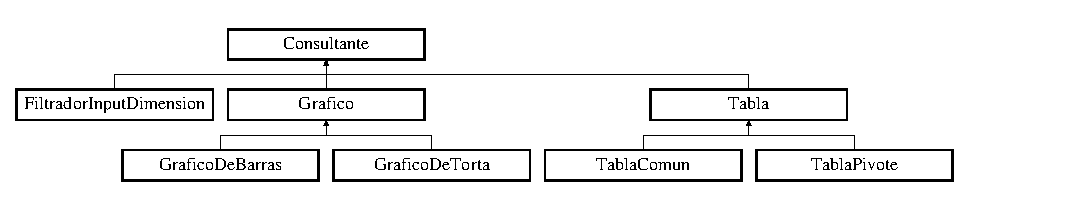
\includegraphics[height=2.196079cm]{classConsultante}
\end{center}
\end{figure}
\subsection*{\-Métodos públicos}
\begin{DoxyCompactItemize}
\item 
\hyperlink{classConsultante_a213165c9f95de185c5ad905ce61b0821}{\-Consultante} ()
\item 
\hyperlink{classConsultante_aaa0291cce87b35d6acc1b6ad1a045b94}{\-Consultante} (\hyperlink{classFiltradoresPanel}{\-Filtradores\-Panel} $\ast$f)
\item 
\hyperlink{classConsultante_afddd574341172d51ef0063b08b336954}{$\sim$\-Consultante} ()
\item 
void \hyperlink{classConsultante_af542575efe45d1c153b4ca76c15e8ebb}{hacer\-Consulta} (\hyperlink{classServidorRemoto}{\-Servidor\-Remoto} \&server)
\item 
void \hyperlink{classConsultante_a3b44313153ac4f5f2859759992657544}{cancelar\-Consulta} (\hyperlink{classServidorRemoto}{\-Servidor\-Remoto} \&server)
\item 
void \hyperlink{classConsultante_af9b4dae4f51439065cf8cac942020409}{recibir\-Respuesta} (const \hyperlink{classRespuesta}{\-Respuesta} \&rta)
\item 
\hypertarget{classConsultante_ad546e54e0a92ea18a21f0f506ecaf4ba}{unsigned {\bfseries get\-I\-D} () const }\label{classConsultante_ad546e54e0a92ea18a21f0f506ecaf4ba}

\item 
\hypertarget{classConsultante_a284fd364766ee4715bb81c4a5e8fc28c}{\hyperlink{classFiltradoresPanel}{\-Filtradores\-Panel} $\ast$ {\bfseries get\-Filtrador} () const }\label{classConsultante_a284fd364766ee4715bb81c4a5e8fc28c}

\item 
\hypertarget{classConsultante_a7d08d916fc29dab431bda10d6b4b080f}{void {\bfseries set\-Spinner} (\-Gtk\-::\-Spinner $\ast$s)}\label{classConsultante_a7d08d916fc29dab431bda10d6b4b080f}

\item 
\hypertarget{classConsultante_aac6df63c36a39a1cf35e8a56145a05a6}{void {\bfseries set\-Padre} (\hyperlink{classTab}{\-Tab} $\ast$padre)}\label{classConsultante_aac6df63c36a39a1cf35e8a56145a05a6}

\item 
\hypertarget{classConsultante_abddbc33c597f6db2b17ada7d011a4c90}{void {\bfseries on\-\_\-navegabilidad\-\_\-seleccionada} ()}\label{classConsultante_abddbc33c597f6db2b17ada7d011a4c90}

\end{DoxyCompactItemize}
\subsection*{\-Métodos protegidos}
\begin{DoxyCompactItemize}
\item 
\hypertarget{classConsultante_ab989a19350df309d7d131cd1daf5e581}{virtual void {\bfseries procesar\-Respuesta} (const \hyperlink{classRespuesta}{\-Respuesta} \&rta)=0}\label{classConsultante_ab989a19350df309d7d131cd1daf5e581}

\item 
\hypertarget{classConsultante_ac0c39ab1e0539a8c80de74d25d2d66de}{void {\bfseries correr\-Spinner} ()}\label{classConsultante_ac0c39ab1e0539a8c80de74d25d2d66de}

\item 
\hypertarget{classConsultante_a26e5dda94d1ad85b10bd192a9e7132b3}{void {\bfseries detener\-Spinner} ()}\label{classConsultante_a26e5dda94d1ad85b10bd192a9e7132b3}

\end{DoxyCompactItemize}
\subsection*{\-Atributos protegidos}
\begin{DoxyCompactItemize}
\item 
\hypertarget{classConsultante_ac21b1a3da7b9024590879d3b202258ea}{\hyperlink{classConsulta}{\-Consulta} {\bfseries consulta}}\label{classConsultante_ac21b1a3da7b9024590879d3b202258ea}

\item 
\hypertarget{classConsultante_ad518d43f57d3a5dcc3390fc8e9c355b9}{\hyperlink{classTab}{\-Tab} $\ast$ {\bfseries padre}}\label{classConsultante_ad518d43f57d3a5dcc3390fc8e9c355b9}

\item 
\hypertarget{classConsultante_afc0f657379fa256784bc65e8bc238725}{\-Gtk\-::\-Spinner $\ast$ {\bfseries spinner}}\label{classConsultante_afc0f657379fa256784bc65e8bc238725}

\end{DoxyCompactItemize}


\subsection{\-Descripción detallada}
\-Clase capaz de armar consultas y enviarlas al servidor que se le solicite.

\-Es el modelo de conexión detrás de las tablas y gráficos y el input por dimensión. \-Controla también el estado de los \-Gtk\-::\-Spinners, un widget informativo para indicar que se espera una respuesta del servidor. 

\subsection{\-Documentación del constructor y destructor}
\hypertarget{classConsultante_a213165c9f95de185c5ad905ce61b0821}{\index{\-Consultante@{\-Consultante}!\-Consultante@{\-Consultante}}
\index{\-Consultante@{\-Consultante}!Consultante@{\-Consultante}}
\subsubsection[{\-Consultante}]{\setlength{\rightskip}{0pt plus 5cm}{\bf \-Consultante\-::\-Consultante} (
\begin{DoxyParamCaption}
{}
\end{DoxyParamCaption}
)}}\label{classConsultante_a213165c9f95de185c5ad905ce61b0821}
\-Constructor. \hypertarget{classConsultante_aaa0291cce87b35d6acc1b6ad1a045b94}{\index{\-Consultante@{\-Consultante}!\-Consultante@{\-Consultante}}
\index{\-Consultante@{\-Consultante}!Consultante@{\-Consultante}}
\subsubsection[{\-Consultante}]{\setlength{\rightskip}{0pt plus 5cm}{\bf \-Consultante\-::\-Consultante} (
\begin{DoxyParamCaption}
\item[{{\bf \-Filtradores\-Panel} $\ast$}]{f}
\end{DoxyParamCaption}
)}}\label{classConsultante_aaa0291cce87b35d6acc1b6ad1a045b94}
\-Constructor. 
\begin{DoxyParams}{\-Parámetros}
{\em f} & conjunto de filtradores asociados \\
\hline
\end{DoxyParams}
\hypertarget{classConsultante_afddd574341172d51ef0063b08b336954}{\index{\-Consultante@{\-Consultante}!$\sim$\-Consultante@{$\sim$\-Consultante}}
\index{$\sim$\-Consultante@{$\sim$\-Consultante}!Consultante@{\-Consultante}}
\subsubsection[{$\sim$\-Consultante}]{\setlength{\rightskip}{0pt plus 5cm}{\bf \-Consultante\-::$\sim$\-Consultante} (
\begin{DoxyParamCaption}
{}
\end{DoxyParamCaption}
)}}\label{classConsultante_afddd574341172d51ef0063b08b336954}
\-Destructor. 

\subsection{\-Documentación de las funciones miembro}
\hypertarget{classConsultante_a3b44313153ac4f5f2859759992657544}{\index{\-Consultante@{\-Consultante}!cancelar\-Consulta@{cancelar\-Consulta}}
\index{cancelar\-Consulta@{cancelar\-Consulta}!Consultante@{\-Consultante}}
\subsubsection[{cancelar\-Consulta}]{\setlength{\rightskip}{0pt plus 5cm}void {\bf \-Consultante\-::cancelar\-Consulta} (
\begin{DoxyParamCaption}
\item[{{\bf \-Servidor\-Remoto} \&}]{server}
\end{DoxyParamCaption}
)}}\label{classConsultante_a3b44313153ac4f5f2859759992657544}
\-Cancela la consulta enviada, e informa al padre que no espera más respuesta. \hypertarget{classConsultante_af542575efe45d1c153b4ca76c15e8ebb}{\index{\-Consultante@{\-Consultante}!hacer\-Consulta@{hacer\-Consulta}}
\index{hacer\-Consulta@{hacer\-Consulta}!Consultante@{\-Consultante}}
\subsubsection[{hacer\-Consulta}]{\setlength{\rightskip}{0pt plus 5cm}void {\bf \-Consultante\-::hacer\-Consulta} (
\begin{DoxyParamCaption}
\item[{{\bf \-Servidor\-Remoto} \&}]{server}
\end{DoxyParamCaption}
)}}\label{classConsultante_af542575efe45d1c153b4ca76c15e8ebb}
\-Envía la consulta, cancelando si ya estaba esperando una respuesta e informa al padre para que pueda controlar su spinner. \hypertarget{classConsultante_af9b4dae4f51439065cf8cac942020409}{\index{\-Consultante@{\-Consultante}!recibir\-Respuesta@{recibir\-Respuesta}}
\index{recibir\-Respuesta@{recibir\-Respuesta}!Consultante@{\-Consultante}}
\subsubsection[{recibir\-Respuesta}]{\setlength{\rightskip}{0pt plus 5cm}void {\bf \-Consultante\-::recibir\-Respuesta} (
\begin{DoxyParamCaption}
\item[{const {\bf \-Respuesta} \&}]{rta}
\end{DoxyParamCaption}
)}}\label{classConsultante_af9b4dae4f51439065cf8cac942020409}
\-Si estaba esperando una respuesta, la procesa. 

\-La documentación para esta clase fue generada a partir de los siguientes ficheros\-:\begin{DoxyCompactItemize}
\item 
cliente/\-Modelo/\-Consultante.\-h\item 
cliente/\-Modelo/\-Consultante.\-cpp\end{DoxyCompactItemize}

\hypertarget{classConsumerConsulta}{\section{\-Referencia de la \-Clase \-Consumer\-Consulta}
\label{classConsumerConsulta}\index{\-Consumer\-Consulta@{\-Consumer\-Consulta}}
}


{\ttfamily \#include $<$\-Consumer\-Consultas.\-h$>$}

\-Diagrama de herencias de \-Consumer\-Consulta\begin{figure}[H]
\begin{center}
\leavevmode
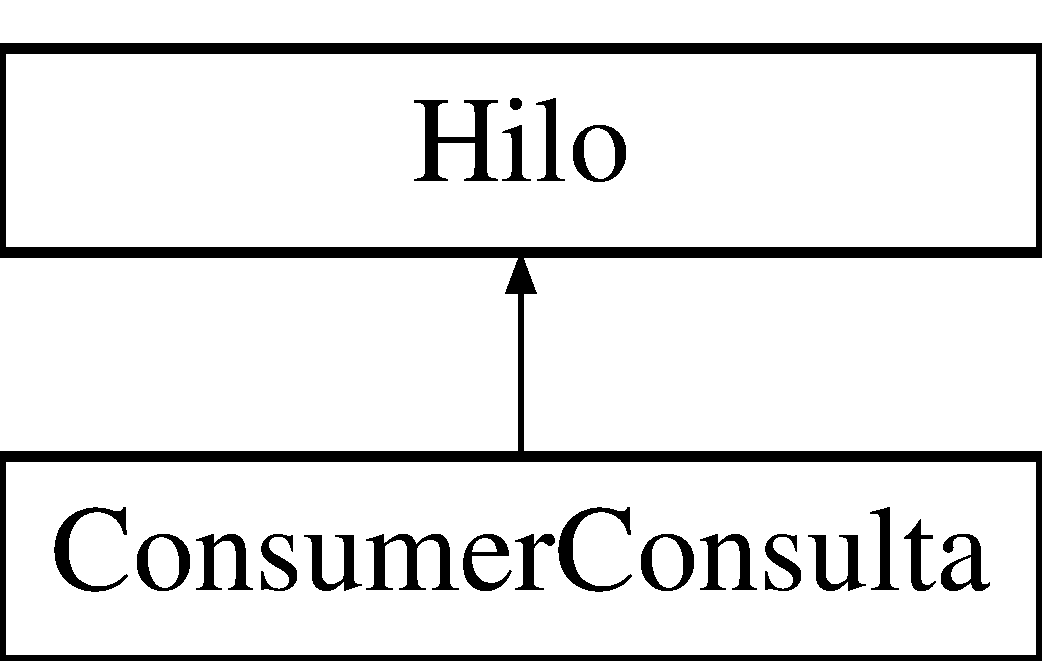
\includegraphics[height=2.000000cm]{classConsumerConsulta}
\end{center}
\end{figure}
\subsection*{\-Métodos públicos}
\begin{DoxyCompactItemize}
\item 
void \hyperlink{classConsumerConsulta_a2ad005877299d61a9f3ba037c1019a02}{correr} ()
\item 
\hyperlink{classConsumerConsulta_ad36f766c49532db3b01b306c70a0e622}{\-Consumer\-Consulta} (\hyperlink{classBLQueue}{\-Cola\-Consultas} \&cons, \hyperlink{classBLQueue}{\-Cola\-Respuestas} \&resp, \hyperlink{classSocket}{\-Socket} $\ast$\&conexion, \hyperlink{classBLMap}{\-Bitmap\-Cancelados} \&canc)
\item 
\hyperlink{classConsumerConsulta_acbed30d06ed4bbeeb4dc5335f042c8c0}{$\sim$\-Consumer\-Consulta} ()
\end{DoxyCompactItemize}


\subsection{\-Descripción detallada}
\-Esta clase es un consumer de consultas. \-Es decir, esta clase tiene como responsabilidad consumir de la cola de consultas del cliente y enviarlas al servidor. \-Al extender de \hyperlink{classHilo}{\-Hilo}, es un thread. \-El consumer se debe sincronizar previo a su destrucción. 

\subsection{\-Documentación del constructor y destructor}
\hypertarget{classConsumerConsulta_ad36f766c49532db3b01b306c70a0e622}{\index{\-Consumer\-Consulta@{\-Consumer\-Consulta}!\-Consumer\-Consulta@{\-Consumer\-Consulta}}
\index{\-Consumer\-Consulta@{\-Consumer\-Consulta}!ConsumerConsulta@{\-Consumer\-Consulta}}
\subsubsection[{\-Consumer\-Consulta}]{\setlength{\rightskip}{0pt plus 5cm}{\bf \-Consumer\-Consulta\-::\-Consumer\-Consulta} (
\begin{DoxyParamCaption}
\item[{{\bf \-Cola\-Consultas} \&}]{cons, }
\item[{{\bf \-Cola\-Respuestas} \&}]{resp, }
\item[{{\bf \-Socket} $\ast$\&}]{conexion, }
\item[{{\bf \-Bitmap\-Cancelados} \&}]{canc}
\end{DoxyParamCaption}
)}}\label{classConsumerConsulta_ad36f766c49532db3b01b306c70a0e622}

\begin{DoxyParams}{\-Parámetros}
{\em cons} & \hyperlink{classReferencia}{\-Referencia} a la cola de consultas del \hyperlink{classServidorRemoto}{\-Servidor\-Remoto}. \\
\hline
{\em resp} & (\-Deprecated) \hyperlink{classReferencia}{\-Referencia} a la cola de respuestas del \hyperlink{classServidorRemoto}{\-Servidor\-Remoto}. \\
\hline
{\em conexion} & \hyperlink{classSocket}{\-Socket} del \hyperlink{classServidorRemoto}{\-Servidor\-Remoto}. \-Por el mismo se envían consultas. \\
\hline
{\em canc} & \-Bitmap de cancelados del \hyperlink{classServidorRemoto}{\-Servidor\-Remoto}. \\
\hline
\end{DoxyParams}
\hypertarget{classConsumerConsulta_acbed30d06ed4bbeeb4dc5335f042c8c0}{\index{\-Consumer\-Consulta@{\-Consumer\-Consulta}!$\sim$\-Consumer\-Consulta@{$\sim$\-Consumer\-Consulta}}
\index{$\sim$\-Consumer\-Consulta@{$\sim$\-Consumer\-Consulta}!ConsumerConsulta@{\-Consumer\-Consulta}}
\subsubsection[{$\sim$\-Consumer\-Consulta}]{\setlength{\rightskip}{0pt plus 5cm}{\bf \-Consumer\-Consulta\-::$\sim$\-Consumer\-Consulta} (
\begin{DoxyParamCaption}
{}
\end{DoxyParamCaption}
)}}\label{classConsumerConsulta_acbed30d06ed4bbeeb4dc5335f042c8c0}
\-Debe sincronizarse el hilo previo a su destrucción. 

\subsection{\-Documentación de las funciones miembro}
\hypertarget{classConsumerConsulta_a2ad005877299d61a9f3ba037c1019a02}{\index{\-Consumer\-Consulta@{\-Consumer\-Consulta}!correr@{correr}}
\index{correr@{correr}!ConsumerConsulta@{\-Consumer\-Consulta}}
\subsubsection[{correr}]{\setlength{\rightskip}{0pt plus 5cm}void {\bf \-Consumer\-Consulta\-::correr} (
\begin{DoxyParamCaption}
{}
\end{DoxyParamCaption}
)\hspace{0.3cm}{\ttfamily  \mbox{[}virtual\mbox{]}}}}\label{classConsumerConsulta_a2ad005877299d61a9f3ba037c1019a02}
\-Es el método llamado por el callback del hilo. \-En el mismo es que se retira de la cola de consultas y se intentan enviar a través del socket. \-Si el envío falla, el hilo detiene su ejecución. 

\-Implementa \hyperlink{classHilo_a187b055e3504487a6bb64340fac2c70d}{\-Hilo}.



\-La documentación para esta clase fue generada a partir de los siguientes ficheros\-:\begin{DoxyCompactItemize}
\item 
cliente/\-Modelo/\-Consumer\-Consultas.\-h\item 
cliente/\-Modelo/\-Consumer\-Consultas.\-cpp\end{DoxyCompactItemize}

\hypertarget{classConsumerRespuesta}{\section{\-Referencia de la \-Clase \-Consumer\-Respuesta}
\label{classConsumerRespuesta}\index{\-Consumer\-Respuesta@{\-Consumer\-Respuesta}}
}


{\ttfamily \#include $<$\-Consumer\-Respuestas.\-h$>$}

\-Diagrama de herencias de \-Consumer\-Respuesta\begin{figure}[H]
\begin{center}
\leavevmode
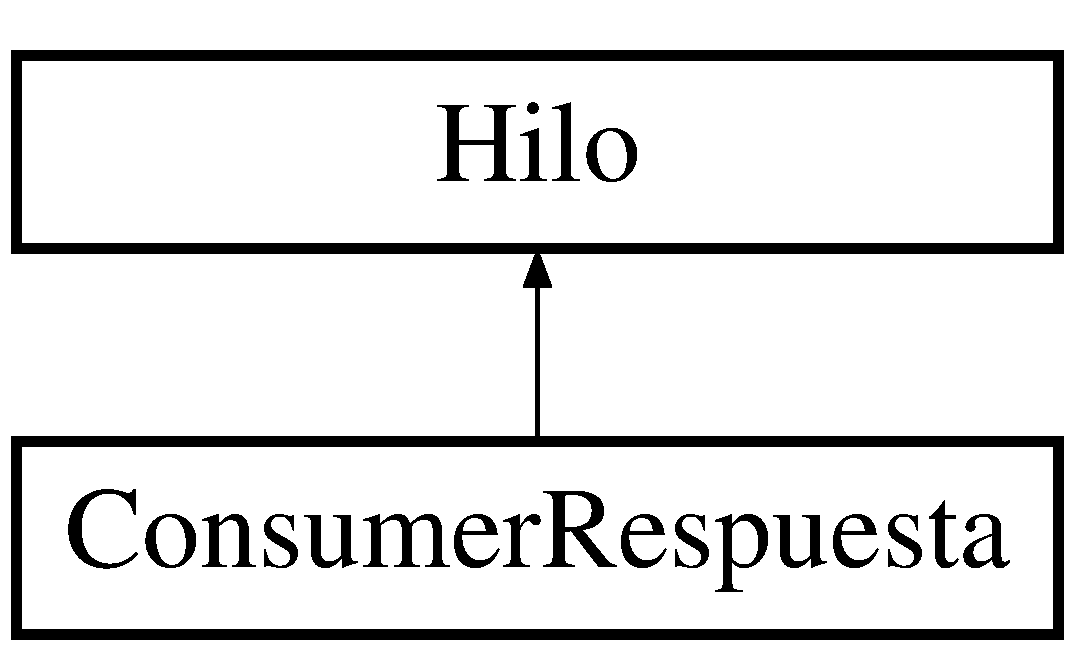
\includegraphics[height=2.000000cm]{classConsumerRespuesta}
\end{center}
\end{figure}
\subsection*{\-Métodos públicos}
\begin{DoxyCompactItemize}
\item 
void \hyperlink{classConsumerRespuesta_a889f4526b5a31e66dfb6eee67552b811}{correr} ()
\item 
\hyperlink{classConsumerRespuesta_a57a2200960ca9cc78a50b2a7188c7970}{\-Consumer\-Respuesta} (\hyperlink{classBLQueue}{\-Cola\-Respuestas} \&cresp, \hyperlink{classBLMap}{\-Mapa\-Consultantes} \&mcons, \hyperlink{classSocket}{\-Socket} $\ast$\&conexion, \hyperlink{classBLMap}{\-Bitmap\-Cancelados} \&canc)
\item 
\hyperlink{classConsumerRespuesta_a6ac047284f3e870a6404b1d77bec88a5}{$\sim$\-Consumer\-Respuesta} ()
\end{DoxyCompactItemize}


\subsection{\-Descripción detallada}
\-Esta clase es un consumer de respuestas. \-Es decir, esta clase tiene como responsabilidad consumir del socket que está conectado al servidor y encolarlas en la cola de respuestas del cliente. \-Al extender de \hyperlink{classHilo}{\-Hilo}, es un thread, entonces el consumer debe ser sincronizado previo a su destrucción. 

\subsection{\-Documentación del constructor y destructor}
\hypertarget{classConsumerRespuesta_a57a2200960ca9cc78a50b2a7188c7970}{\index{\-Consumer\-Respuesta@{\-Consumer\-Respuesta}!\-Consumer\-Respuesta@{\-Consumer\-Respuesta}}
\index{\-Consumer\-Respuesta@{\-Consumer\-Respuesta}!ConsumerRespuesta@{\-Consumer\-Respuesta}}
\subsubsection[{\-Consumer\-Respuesta}]{\setlength{\rightskip}{0pt plus 5cm}{\bf \-Consumer\-Respuesta\-::\-Consumer\-Respuesta} (
\begin{DoxyParamCaption}
\item[{{\bf \-Cola\-Respuestas} \&}]{cresp, }
\item[{{\bf \-Mapa\-Consultantes} \&}]{mcons, }
\item[{{\bf \-Socket} $\ast$\&}]{conexion, }
\item[{{\bf \-Bitmap\-Cancelados} \&}]{canc}
\end{DoxyParamCaption}
)}}\label{classConsumerRespuesta_a57a2200960ca9cc78a50b2a7188c7970}

\begin{DoxyParams}{\-Parámetros}
{\em cresp} & \-Cola de respuestas del servidor. \\
\hline
{\em mcons} & (deprecated) mapa de consultantes del servidor. \\
\hline
{\em conexion} & \hyperlink{classSocket}{\-Socket} del \hyperlink{classServidorRemoto}{\-Servidor\-Remoto} conectado al servidor. \\
\hline
{\em canc} & \-Bitmap de consultas canceladas. \\
\hline
\end{DoxyParams}
\hypertarget{classConsumerRespuesta_a6ac047284f3e870a6404b1d77bec88a5}{\index{\-Consumer\-Respuesta@{\-Consumer\-Respuesta}!$\sim$\-Consumer\-Respuesta@{$\sim$\-Consumer\-Respuesta}}
\index{$\sim$\-Consumer\-Respuesta@{$\sim$\-Consumer\-Respuesta}!ConsumerRespuesta@{\-Consumer\-Respuesta}}
\subsubsection[{$\sim$\-Consumer\-Respuesta}]{\setlength{\rightskip}{0pt plus 5cm}{\bf \-Consumer\-Respuesta\-::$\sim$\-Consumer\-Respuesta} (
\begin{DoxyParamCaption}
{}
\end{DoxyParamCaption}
)}}\label{classConsumerRespuesta_a6ac047284f3e870a6404b1d77bec88a5}
\-Debe sincronizarse el hilo antes de ser destruido. 

\subsection{\-Documentación de las funciones miembro}
\hypertarget{classConsumerRespuesta_a889f4526b5a31e66dfb6eee67552b811}{\index{\-Consumer\-Respuesta@{\-Consumer\-Respuesta}!correr@{correr}}
\index{correr@{correr}!ConsumerRespuesta@{\-Consumer\-Respuesta}}
\subsubsection[{correr}]{\setlength{\rightskip}{0pt plus 5cm}void {\bf \-Consumer\-Respuesta\-::correr} (
\begin{DoxyParamCaption}
{}
\end{DoxyParamCaption}
)\hspace{0.3cm}{\ttfamily  \mbox{[}virtual\mbox{]}}}}\label{classConsumerRespuesta_a889f4526b5a31e66dfb6eee67552b811}
\-Es el método llamado por el callback del hilo. \-En el mismo se espera por una respuesta del socket. \-Si recibe exitosamente encola la respuesta en la cola de respuestas del cliente. \-Si falla la recepción, el hilo procederá a detener su ejecución. 

\-Implementa \hyperlink{classHilo_a187b055e3504487a6bb64340fac2c70d}{\-Hilo}.



\-La documentación para esta clase fue generada a partir de los siguientes ficheros\-:\begin{DoxyCompactItemize}
\item 
cliente/\-Modelo/\-Consumer\-Respuestas.\-h\item 
cliente/\-Modelo/\-Consumer\-Respuestas.\-cpp\end{DoxyCompactItemize}

\hypertarget{classConsumidor}{\section{\-Referencia de la \-Clase \-Consumidor}
\label{classConsumidor}\index{\-Consumidor@{\-Consumidor}}
}
\-Diagrama de herencias de \-Consumidor\begin{figure}[H]
\begin{center}
\leavevmode
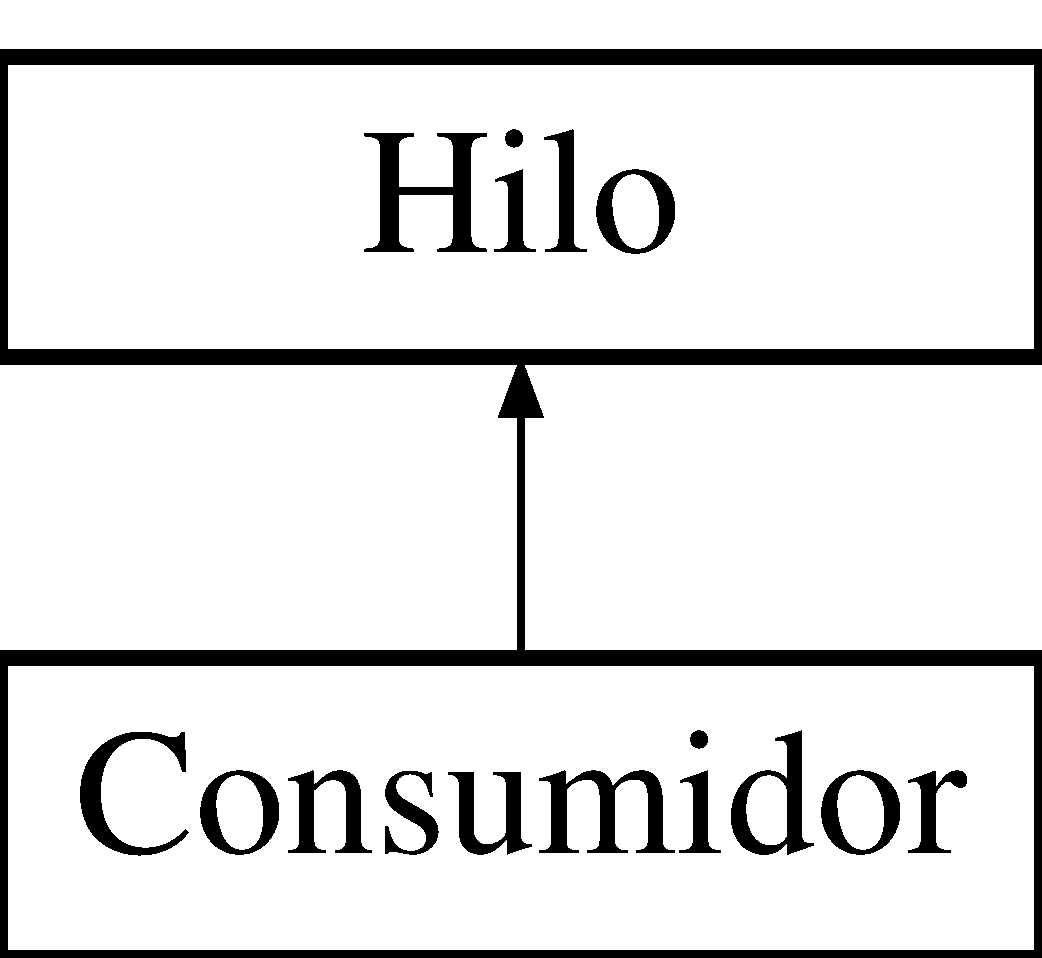
\includegraphics[height=2.000000cm]{classConsumidor}
\end{center}
\end{figure}
\subsection*{\-Métodos públicos}
\begin{DoxyCompactItemize}
\item 
\hypertarget{classConsumidor_af4e98de3f07fe279bef37803d60966c7}{{\bfseries \-Consumidor} (\hyperlink{classBLQueue}{\-Cola\-Prueba} \&c, int id)}\label{classConsumidor_af4e98de3f07fe279bef37803d60966c7}

\item 
\hypertarget{classConsumidor_a24aa380e7122221c06549d1eb59f1c4e}{virtual void \hyperlink{classConsumidor_a24aa380e7122221c06549d1eb59f1c4e}{correr} ()}\label{classConsumidor_a24aa380e7122221c06549d1eb59f1c4e}

\begin{DoxyCompactList}\small\item\em \-Metodo virtual puro, que corre cuando se ejecuta el hilo. \end{DoxyCompactList}\end{DoxyCompactItemize}
\subsection*{\-Atributos públicos}
\begin{DoxyCompactItemize}
\item 
\hypertarget{classConsumidor_a9a6fd3586c1b4ca2063557a05c606c77}{int {\bfseries \-\_\-id}}\label{classConsumidor_a9a6fd3586c1b4ca2063557a05c606c77}

\item 
\hypertarget{classConsumidor_a7f4e73a75d0b0aa8c82ce1f696cc794e}{\hyperlink{classBLQueue}{\-Cola\-Prueba} \& {\bfseries cola}}\label{classConsumidor_a7f4e73a75d0b0aa8c82ce1f696cc794e}

\end{DoxyCompactItemize}


\-La documentación para esta clase fue generada a partir del siguiente fichero\-:\begin{DoxyCompactItemize}
\item 
servidor/test.\-cpp\end{DoxyCompactItemize}

\hypertarget{classContenedorAgentes}{\section{\-Referencia de la \-Clase \-Contenedor\-Agentes}
\label{classContenedorAgentes}\index{\-Contenedor\-Agentes@{\-Contenedor\-Agentes}}
}


{\ttfamily \#include $<$\-Contenedor\-Agentes.\-h$>$}

\-Diagrama de herencias de \-Contenedor\-Agentes\begin{figure}[H]
\begin{center}
\leavevmode
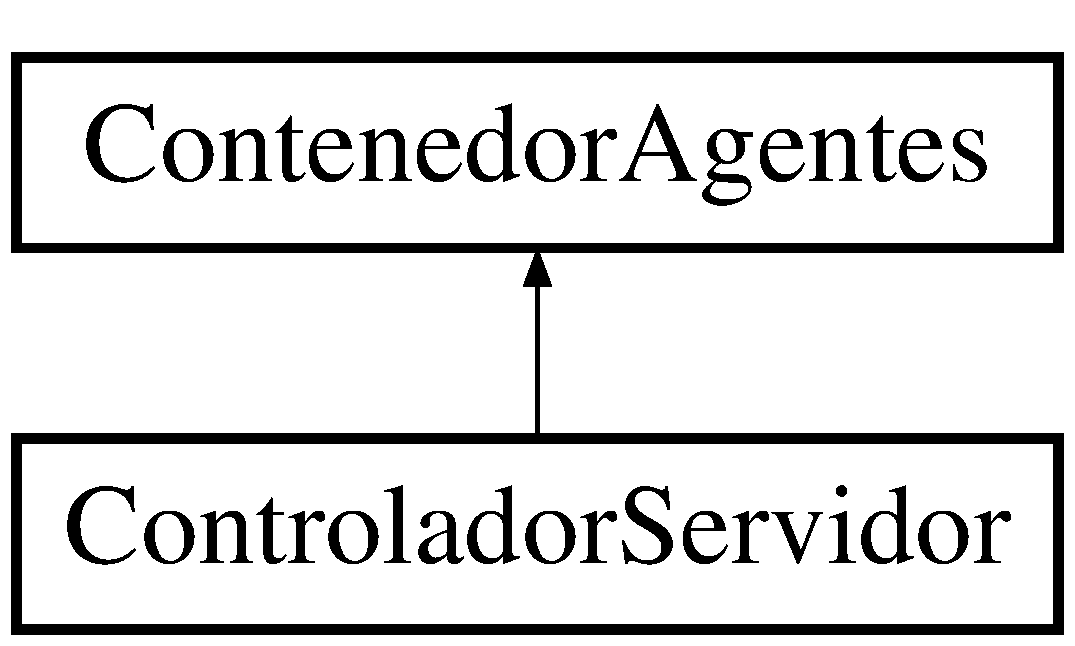
\includegraphics[height=2.000000cm]{classContenedorAgentes}
\end{center}
\end{figure}
\subsection*{\-Métodos públicos}
\begin{DoxyCompactItemize}
\item 
virtual void \hyperlink{classContenedorAgentes_a5e701061672c9cb813fc468a79979475}{agregar\-Agente} (\hyperlink{classAgenteRemoto}{\-Agente\-Remoto} $\ast$agt)=0
\end{DoxyCompactItemize}


\subsection{\-Descripción detallada}
\-Es una clase que hace de interfaz a un objeto que pueda contener a los agentes remotos. \-La misma será utilizada por el controlador del servidor que los contendrá a todos. \-Sirve para mitigar el acoplamiento. 

\subsection{\-Documentación de las funciones miembro}
\hypertarget{classContenedorAgentes_a5e701061672c9cb813fc468a79979475}{\index{\-Contenedor\-Agentes@{\-Contenedor\-Agentes}!agregar\-Agente@{agregar\-Agente}}
\index{agregar\-Agente@{agregar\-Agente}!ContenedorAgentes@{\-Contenedor\-Agentes}}
\subsubsection[{agregar\-Agente}]{\setlength{\rightskip}{0pt plus 5cm}virtual void {\bf \-Contenedor\-Agentes\-::agregar\-Agente} (
\begin{DoxyParamCaption}
\item[{{\bf \-Agente\-Remoto} $\ast$}]{agt}
\end{DoxyParamCaption}
)\hspace{0.3cm}{\ttfamily  \mbox{[}pure virtual\mbox{]}}}}\label{classContenedorAgentes_a5e701061672c9cb813fc468a79979475}
\-Metodo virtual abstracto que debe implementar cada contenedor. 

\-Implementado en \hyperlink{classControladorServidor_ad323cf3309ee0ddc8737c16a48432c28}{\-Controlador\-Servidor}.



\-La documentación para esta clase fue generada a partir del siguiente fichero\-:\begin{DoxyCompactItemize}
\item 
servidor/servidor/\-Contenedor\-Agentes.\-h\end{DoxyCompactItemize}

\hypertarget{classContenedorClientes}{\section{\-Referencia de la \-Clase \-Contenedor\-Clientes}
\label{classContenedorClientes}\index{\-Contenedor\-Clientes@{\-Contenedor\-Clientes}}
}


{\ttfamily \#include $<$\-Contenedor\-Clientes.\-h$>$}

\-Diagrama de herencias de \-Contenedor\-Clientes\begin{figure}[H]
\begin{center}
\leavevmode
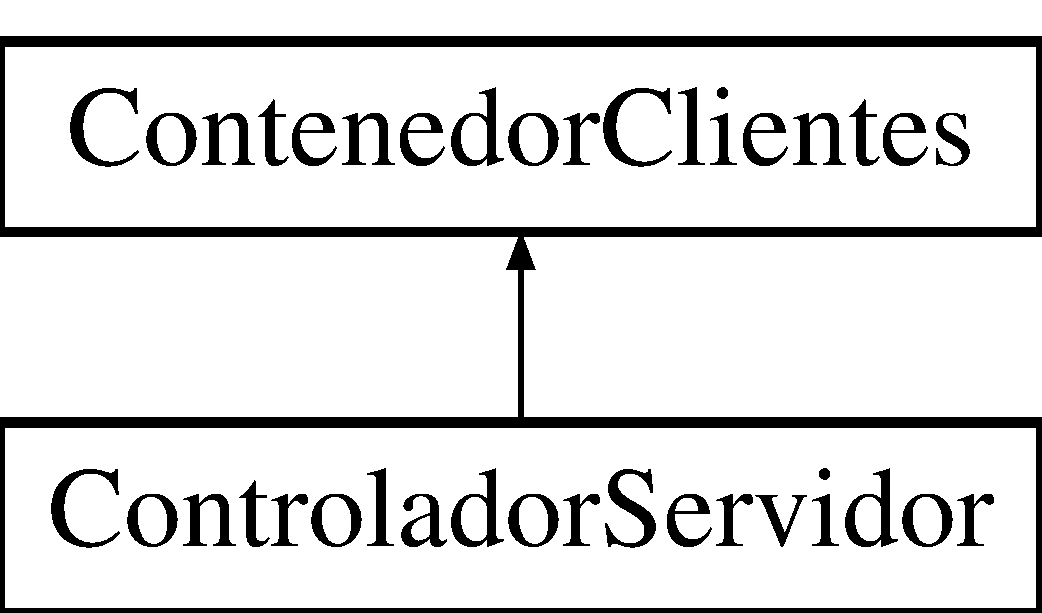
\includegraphics[height=2.000000cm]{classContenedorClientes}
\end{center}
\end{figure}
\subsection*{\-Métodos públicos}
\begin{DoxyCompactItemize}
\item 
\hypertarget{classContenedorClientes_a87f11c5cf6e9259a9a79cb42a0a6f363}{virtual void {\bfseries agregar\-Cliente} (\hyperlink{classClienteRemoto}{\-Cliente\-Remoto} $\ast$agt)=0}\label{classContenedorClientes_a87f11c5cf6e9259a9a79cb42a0a6f363}

\end{DoxyCompactItemize}


\subsection{\-Descripción detallada}
\-Es una clase que hace de interfaz a un objeto que pueda contener a los clientes remotos. \-La misma será uitlizada por el controlador del servidor que los contendrá a todos. \-Sirve para mitigar el acoplamiento. 

\-La documentación para esta clase fue generada a partir del siguiente fichero\-:\begin{DoxyCompactItemize}
\item 
servidor/servidor/\-Contenedor\-Clientes.\-h\end{DoxyCompactItemize}

\hypertarget{classControladorServidor}{\section{\-Referencia de la \-Clase \-Controlador\-Servidor}
\label{classControladorServidor}\index{\-Controlador\-Servidor@{\-Controlador\-Servidor}}
}


{\ttfamily \#include $<$\-Controlador\-Servidor.\-h$>$}

\-Diagrama de herencias de \-Controlador\-Servidor\begin{figure}[H]
\begin{center}
\leavevmode
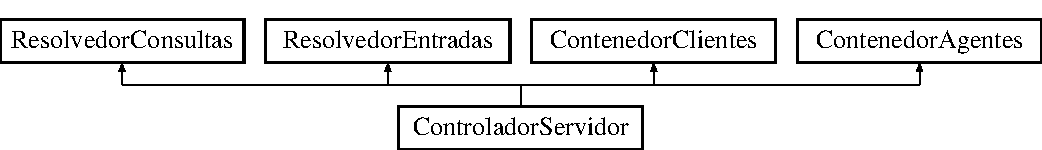
\includegraphics[height=2.000000cm]{classControladorServidor}
\end{center}
\end{figure}
\subsection*{\-Métodos públicos}
\begin{DoxyCompactItemize}
\item 
\hyperlink{classRespuesta}{\-Respuesta} \hyperlink{classControladorServidor_a45d1f810987e11a222986ecf588ac497}{resolver\-Entrada} (\hyperlink{classConsulta}{\-Consulta} \&entrada)
\item 
\hyperlink{classRespuesta}{\-Respuesta} \hyperlink{classControladorServidor_a1ca5d73913116531b23e8c998f51f18b}{resolver} (\hyperlink{classConsulta}{\-Consulta} \&consulta)
\item 
\hyperlink{classControladorServidor_a62668a91f2eeb6fe13d7a4079e023ac8}{\-Controlador\-Servidor} (\hyperlink{classResolvedorConsultas}{\-Resolvedor\-Consultas} \&cons, \hyperlink{classResolvedorEntradas}{\-Resolvedor\-Entradas} \&rent, \-Puerto pclientes, \-Puerto pagentes)
\item 
bool \hyperlink{classControladorServidor_a492e61d31b759540ec76a1ca2c7bb875}{activo} ()
\item 
\hyperlink{classControladorServidor_abe83c8c099a41bae0ff648e0b7281741}{$\sim$\-Controlador\-Servidor} ()
\item 
void \hyperlink{classControladorServidor_aaa97dc23fdf70cf91004bdb654b72585}{agregar\-Cliente} (\hyperlink{classClienteRemoto}{\-Cliente\-Remoto} $\ast$rem)
\item 
void \hyperlink{classControladorServidor_ad323cf3309ee0ddc8737c16a48432c28}{agregar\-Agente} (\hyperlink{classAgenteRemoto}{\-Agente\-Remoto} $\ast$agt)
\item 
void \hyperlink{classControladorServidor_aa50662d57613d4e161790f6e9dc1c299}{comenzar} ()
\item 
void \hyperlink{classControladorServidor_aa8f33c7beb356148089072234a2619b4}{detener} ()
\end{DoxyCompactItemize}


\subsection{\-Descripción detallada}
\-Esta clase es fundamental. \-Su rol es controlar el flujo correcto de resolución de consultas y actualizaciones. \-Se encarga de permitir que el servidor maneje múltiples consultas, como también de frenarlas cuando se requiera de procesar actualizaciones. \-Contiene un \-Pool de \char`\"{}workers\char`\"{}, cada uno con una dedicación a alguna de las tareas ya sean de actualización como de consultas. \-Implementa interfaces como \hyperlink{classResolvedorConsultas}{\-Resolvedor\-Consultas}, \hyperlink{classResolvedorEntradas}{\-Resolvedor\-Entradas}, \hyperlink{classContenedorClientes}{\-Contenedor\-Clientes} y \hyperlink{classContenedorAgentes}{\-Contenedor\-Agentes}, que hace que sus \char`\"{}workers\char`\"{} sólo vean lo que necesiten ver del controlador.

\-Es la clase encargada también de manejar los hilos que se encargan de recibir clientes y agentes. \-En definitiva, es el encargado de la coordinacion de la concurrencia del servidor. 

\subsection{\-Documentación del constructor y destructor}
\hypertarget{classControladorServidor_a62668a91f2eeb6fe13d7a4079e023ac8}{\index{\-Controlador\-Servidor@{\-Controlador\-Servidor}!\-Controlador\-Servidor@{\-Controlador\-Servidor}}
\index{\-Controlador\-Servidor@{\-Controlador\-Servidor}!ControladorServidor@{\-Controlador\-Servidor}}
\subsubsection[{\-Controlador\-Servidor}]{\setlength{\rightskip}{0pt plus 5cm}{\bf \-Controlador\-Servidor\-::\-Controlador\-Servidor} (
\begin{DoxyParamCaption}
\item[{{\bf \-Resolvedor\-Consultas} \&}]{cons, }
\item[{{\bf \-Resolvedor\-Entradas} \&}]{rent, }
\item[{\-Puerto}]{pclientes, }
\item[{\-Puerto}]{pagentes}
\end{DoxyParamCaption}
)}}\label{classControladorServidor_a62668a91f2eeb6fe13d7a4079e023ac8}
\-Constructor de controlador\-Servidor. 
\begin{DoxyParams}{\-Parámetros}
{\em cons} & \-Objeto que resuelva las consultas. \\
\hline
{\em rent} & \-Objeto que resuelva las entradas. \\
\hline
{\em pclientes} & \-Puerto por el cual se escucharán conexiones entrantes de los clientes. \\
\hline
{\em pagentes} & \-Puerto por el cual se escucharán conexiones entrantes de los agentes. \\
\hline
\end{DoxyParams}
\hypertarget{classControladorServidor_abe83c8c099a41bae0ff648e0b7281741}{\index{\-Controlador\-Servidor@{\-Controlador\-Servidor}!$\sim$\-Controlador\-Servidor@{$\sim$\-Controlador\-Servidor}}
\index{$\sim$\-Controlador\-Servidor@{$\sim$\-Controlador\-Servidor}!ControladorServidor@{\-Controlador\-Servidor}}
\subsubsection[{$\sim$\-Controlador\-Servidor}]{\setlength{\rightskip}{0pt plus 5cm}{\bf \-Controlador\-Servidor\-::$\sim$\-Controlador\-Servidor} (
\begin{DoxyParamCaption}
{}
\end{DoxyParamCaption}
)}}\label{classControladorServidor_abe83c8c099a41bae0ff648e0b7281741}
\-El destructor del controlador. \-Si esta en ejecución, libera toda la memoria que corresponda, cerrando conexiones y deteniendo hilos. 

\subsection{\-Documentación de las funciones miembro}
\hypertarget{classControladorServidor_a492e61d31b759540ec76a1ca2c7bb875}{\index{\-Controlador\-Servidor@{\-Controlador\-Servidor}!activo@{activo}}
\index{activo@{activo}!ControladorServidor@{\-Controlador\-Servidor}}
\subsubsection[{activo}]{\setlength{\rightskip}{0pt plus 5cm}bool {\bf \-Controlador\-Servidor\-::activo} (
\begin{DoxyParamCaption}
{}
\end{DoxyParamCaption}
)}}\label{classControladorServidor_a492e61d31b759540ec76a1ca2c7bb875}
\-Método utilizado para saber si las entradas siguen activas. \hypertarget{classControladorServidor_ad323cf3309ee0ddc8737c16a48432c28}{\index{\-Controlador\-Servidor@{\-Controlador\-Servidor}!agregar\-Agente@{agregar\-Agente}}
\index{agregar\-Agente@{agregar\-Agente}!ControladorServidor@{\-Controlador\-Servidor}}
\subsubsection[{agregar\-Agente}]{\setlength{\rightskip}{0pt plus 5cm}void {\bf \-Controlador\-Servidor\-::agregar\-Agente} (
\begin{DoxyParamCaption}
\item[{{\bf \-Agente\-Remoto} $\ast$}]{agt}
\end{DoxyParamCaption}
)\hspace{0.3cm}{\ttfamily  \mbox{[}virtual\mbox{]}}}}\label{classControladorServidor_ad323cf3309ee0ddc8737c16a48432c28}
\-El método que permite agregar un agente remoto a su lista. \-Es el heredado de la interfaz \hyperlink{classContenedorAgentes}{\-Contenedor\-Agentes}. 

\-Implementa \hyperlink{classContenedorAgentes_a5e701061672c9cb813fc468a79979475}{\-Contenedor\-Agentes}.

\hypertarget{classControladorServidor_aaa97dc23fdf70cf91004bdb654b72585}{\index{\-Controlador\-Servidor@{\-Controlador\-Servidor}!agregar\-Cliente@{agregar\-Cliente}}
\index{agregar\-Cliente@{agregar\-Cliente}!ControladorServidor@{\-Controlador\-Servidor}}
\subsubsection[{agregar\-Cliente}]{\setlength{\rightskip}{0pt plus 5cm}void {\bf \-Controlador\-Servidor\-::agregar\-Cliente} (
\begin{DoxyParamCaption}
\item[{{\bf \-Cliente\-Remoto} $\ast$}]{rem}
\end{DoxyParamCaption}
)\hspace{0.3cm}{\ttfamily  \mbox{[}virtual\mbox{]}}}}\label{classControladorServidor_aaa97dc23fdf70cf91004bdb654b72585}
\-El método que permite agregar un cliente remoto a su lista. \-Es el heredado de la interfaz \hyperlink{classContenedorClientes}{\-Contenedor\-Clientes}. 

\-Implementa \hyperlink{classContenedorClientes}{\-Contenedor\-Clientes}.

\hypertarget{classControladorServidor_aa50662d57613d4e161790f6e9dc1c299}{\index{\-Controlador\-Servidor@{\-Controlador\-Servidor}!comenzar@{comenzar}}
\index{comenzar@{comenzar}!ControladorServidor@{\-Controlador\-Servidor}}
\subsubsection[{comenzar}]{\setlength{\rightskip}{0pt plus 5cm}void {\bf \-Controlador\-Servidor\-::comenzar} (
\begin{DoxyParamCaption}
{}
\end{DoxyParamCaption}
)}}\label{classControladorServidor_aa50662d57613d4e161790f6e9dc1c299}
\-Se encarga de inicar los hilos correspondientes a los que escuchan conexiones y a los pools de workers. \hypertarget{classControladorServidor_aa8f33c7beb356148089072234a2619b4}{\index{\-Controlador\-Servidor@{\-Controlador\-Servidor}!detener@{detener}}
\index{detener@{detener}!ControladorServidor@{\-Controlador\-Servidor}}
\subsubsection[{detener}]{\setlength{\rightskip}{0pt plus 5cm}void {\bf \-Controlador\-Servidor\-::detener} (
\begin{DoxyParamCaption}
{}
\end{DoxyParamCaption}
)}}\label{classControladorServidor_aa8f33c7beb356148089072234a2619b4}
\-Se encarga de detener todos los hilos, tanto los workers como los que escuchan conexiones ingresantes, cierra las colas de consultas y realiza tareas varias previas a la destruccion del mismo. \hypertarget{classControladorServidor_a1ca5d73913116531b23e8c998f51f18b}{\index{\-Controlador\-Servidor@{\-Controlador\-Servidor}!resolver@{resolver}}
\index{resolver@{resolver}!ControladorServidor@{\-Controlador\-Servidor}}
\subsubsection[{resolver}]{\setlength{\rightskip}{0pt plus 5cm}{\bf \-Respuesta} {\bf \-Controlador\-Servidor\-::resolver} (
\begin{DoxyParamCaption}
\item[{{\bf \-Consulta} \&}]{consulta}
\end{DoxyParamCaption}
)\hspace{0.3cm}{\ttfamily  \mbox{[}virtual\mbox{]}}}}\label{classControladorServidor_a1ca5d73913116531b23e8c998f51f18b}
\-Este método es el encargado de resolver las consultas. \-Si hay entradas resolviéndose en el momento de la llamada, este método quedará bloqueado hasta que pueda realizar la consulta. \-Sin embargo no se bloqueara si otras consultas están en proceso, permitiendo la resolución de consultas de forma concurrente. 

\-Implementa \hyperlink{classResolvedorConsultas_a077d3d962848e14a84790d5a929fea17}{\-Resolvedor\-Consultas}.

\hypertarget{classControladorServidor_a45d1f810987e11a222986ecf588ac497}{\index{\-Controlador\-Servidor@{\-Controlador\-Servidor}!resolver\-Entrada@{resolver\-Entrada}}
\index{resolver\-Entrada@{resolver\-Entrada}!ControladorServidor@{\-Controlador\-Servidor}}
\subsubsection[{resolver\-Entrada}]{\setlength{\rightskip}{0pt plus 5cm}{\bf \-Respuesta} {\bf \-Controlador\-Servidor\-::resolver\-Entrada} (
\begin{DoxyParamCaption}
\item[{{\bf \-Consulta} \&}]{entrada}
\end{DoxyParamCaption}
)\hspace{0.3cm}{\ttfamily  \mbox{[}virtual\mbox{]}}}}\label{classControladorServidor_a45d1f810987e11a222986ecf588ac497}
\-Este método es el encargado de resolver las actualizaciones. \-Si hay consultas resolviéndose en el momento de la llamada, quedará bloqueado hasta que pueda realizar la actualización. 

\-Implementa \hyperlink{classResolvedorEntradas_a197be7d4db0a07250a51c2c390dd2372}{\-Resolvedor\-Entradas}.



\-La documentación para esta clase fue generada a partir de los siguientes ficheros\-:\begin{DoxyCompactItemize}
\item 
servidor/servidor/\-Controlador\-Servidor.\-h\item 
servidor/servidor/\-Controlador\-Servidor.\-cpp\end{DoxyCompactItemize}

\hypertarget{classDialogoAutentif}{\section{\-Referencia de la \-Clase \-Dialogo\-Autentif}
\label{classDialogoAutentif}\index{\-Dialogo\-Autentif@{\-Dialogo\-Autentif}}
}


{\ttfamily \#include $<$\-Dialogo\-Autentif.\-h$>$}

\-Diagrama de herencias de \-Dialogo\-Autentif\begin{figure}[H]
\begin{center}
\leavevmode
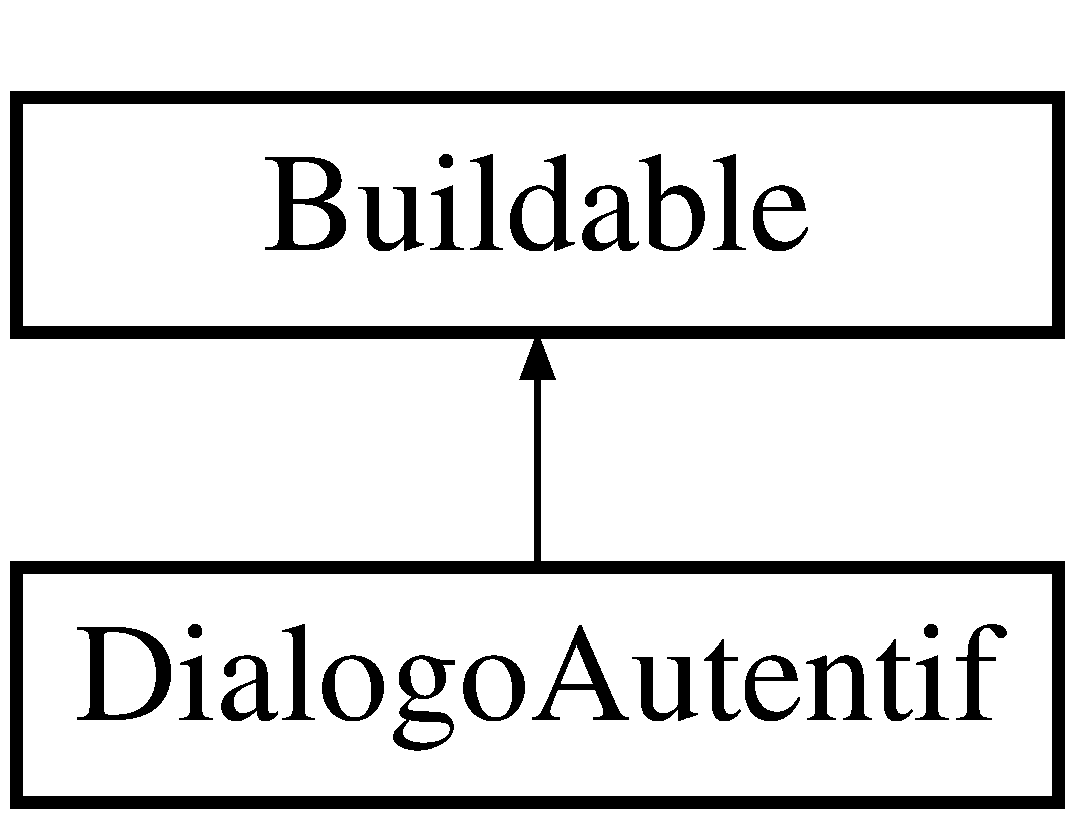
\includegraphics[height=2.000000cm]{classDialogoAutentif}
\end{center}
\end{figure}
\subsection*{\-Métodos públicos}
\begin{DoxyCompactItemize}
\item 
\hyperlink{classDialogoAutentif_a249ccc61d65b6f2648fa2d6ab45e9031}{\-Dialogo\-Autentif} (\-Base\-Object\-Type $\ast$cobject, const \-Glib\-::\-Ref\-Ptr$<$ \-Gtk\-::\-Builder $>$ \&builder)
\item 
\hyperlink{classDialogoAutentif_a8c721f31adfd29a1d82647aac2d79b8b}{$\sim$\-Dialogo\-Autentif} ()
\end{DoxyCompactItemize}


\subsection{\-Descripción detallada}
\-Esta clase agrupa las cosas mínimas necesarias para restringir acceso. \-Solicita el password de acceso, y retorna éxito o fracaso en la autentificación. 

\subsection{\-Documentación del constructor y destructor}
\hypertarget{classDialogoAutentif_a249ccc61d65b6f2648fa2d6ab45e9031}{\index{\-Dialogo\-Autentif@{\-Dialogo\-Autentif}!\-Dialogo\-Autentif@{\-Dialogo\-Autentif}}
\index{\-Dialogo\-Autentif@{\-Dialogo\-Autentif}!DialogoAutentif@{\-Dialogo\-Autentif}}
\subsubsection[{\-Dialogo\-Autentif}]{\setlength{\rightskip}{0pt plus 5cm}{\bf \-Dialogo\-Autentif\-::\-Dialogo\-Autentif} (
\begin{DoxyParamCaption}
\item[{\-Base\-Object\-Type $\ast$}]{cobject, }
\item[{const \-Glib\-::\-Ref\-Ptr$<$ \-Gtk\-::\-Builder $>$ \&}]{builder}
\end{DoxyParamCaption}
)}}\label{classDialogoAutentif_a249ccc61d65b6f2648fa2d6ab45e9031}
\-Constructor requerido para construir con \-Gtk\-::\-Builder. 
\begin{DoxyParams}{\-Parámetros}
{\em cobject} & puntero al tipo base \\
\hline
{\em builder} & referencia a la instancia que lo construye \\
\hline
\end{DoxyParams}
\hypertarget{classDialogoAutentif_a8c721f31adfd29a1d82647aac2d79b8b}{\index{\-Dialogo\-Autentif@{\-Dialogo\-Autentif}!$\sim$\-Dialogo\-Autentif@{$\sim$\-Dialogo\-Autentif}}
\index{$\sim$\-Dialogo\-Autentif@{$\sim$\-Dialogo\-Autentif}!DialogoAutentif@{\-Dialogo\-Autentif}}
\subsubsection[{$\sim$\-Dialogo\-Autentif}]{\setlength{\rightskip}{0pt plus 5cm}{\bf \-Dialogo\-Autentif\-::$\sim$\-Dialogo\-Autentif} (
\begin{DoxyParamCaption}
{}
\end{DoxyParamCaption}
)}}\label{classDialogoAutentif_a8c721f31adfd29a1d82647aac2d79b8b}
\-Destructor. 

\-La documentación para esta clase fue generada a partir de los siguientes ficheros\-:\begin{DoxyCompactItemize}
\item 
cliente/\-Vista/\-Dialogo\-Autentif.\-h\item 
cliente/\-Vista/\-Dialogo\-Autentif.\-cpp\end{DoxyCompactItemize}

\hypertarget{classErrorAperturaServidor}{\section{\-Referencia de la \-Clase \-Error\-Apertura\-Servidor}
\label{classErrorAperturaServidor}\index{\-Error\-Apertura\-Servidor@{\-Error\-Apertura\-Servidor}}
}


\-La documentación para esta clase fue generada a partir del siguiente fichero\-:\begin{DoxyCompactItemize}
\item 
servidor/\-Errores/\-Error\-Apertura\-Servidor.\-h\end{DoxyCompactItemize}

\hypertarget{classErrorArchivoCorrompido}{\section{\-Referencia de la \-Clase \-Error\-Archivo\-Corrompido}
\label{classErrorArchivoCorrompido}\index{\-Error\-Archivo\-Corrompido@{\-Error\-Archivo\-Corrompido}}
}


\-La documentación para esta clase fue generada a partir del siguiente fichero\-:\begin{DoxyCompactItemize}
\item 
servidor/\-Motor\-De\-Consultas/\-Error\-Archivo\-Corrompido.\-h\end{DoxyCompactItemize}

\hypertarget{classErrorOrganizacion}{\section{\-Referencia de la \-Clase \-Error\-Organizacion}
\label{classErrorOrganizacion}\index{\-Error\-Organizacion@{\-Error\-Organizacion}}
}


\-La documentación para esta clase fue generada a partir del siguiente fichero\-:\begin{DoxyCompactItemize}
\item 
comun/\-Error\-Organizacion.\-h\end{DoxyCompactItemize}

\hypertarget{classErrorPersistencia}{\section{\-Referencia de la \-Clase \-Error\-Persistencia}
\label{classErrorPersistencia}\index{\-Error\-Persistencia@{\-Error\-Persistencia}}
}


\-La documentación para esta clase fue generada a partir del siguiente fichero\-:\begin{DoxyCompactItemize}
\item 
servidor/\-Errores/\-Error\-Persistencia.\-h\end{DoxyCompactItemize}

\hypertarget{classErrorSerializacionXML}{\section{\-Referencia de la \-Clase \-Error\-Serializacion\-X\-M\-L}
\label{classErrorSerializacionXML}\index{\-Error\-Serializacion\-X\-M\-L@{\-Error\-Serializacion\-X\-M\-L}}
}


\-La documentación para esta clase fue generada a partir del siguiente fichero\-:\begin{DoxyCompactItemize}
\item 
cliente/\-Modelo/\-Definiciones\-X\-M\-L.\-h\end{DoxyCompactItemize}

\hypertarget{classExcepcionArchivoGladeCorrupto}{\section{\-Referencia de la \-Clase \-Excepcion\-Archivo\-Glade\-Corrupto}
\label{classExcepcionArchivoGladeCorrupto}\index{\-Excepcion\-Archivo\-Glade\-Corrupto@{\-Excepcion\-Archivo\-Glade\-Corrupto}}
}


{\ttfamily \#include $<$\-Excepcion\-Archivo\-Glade\-Corrupto.\-h$>$}

\subsection*{\-Métodos públicos}
\begin{DoxyCompactItemize}
\item 
\hyperlink{classExcepcionArchivoGladeCorrupto_a9732a4d8b31b19b66326b3efc6a40c71}{\-Excepcion\-Archivo\-Glade\-Corrupto} (const std\-::string \&\-\_\-msj)
\item 
\hyperlink{classExcepcionArchivoGladeCorrupto_ae2170588abaf5ecf4b45fbeb7d62846b}{$\sim$\-Excepcion\-Archivo\-Glade\-Corrupto} ()  throw ()
\item 
\hypertarget{classExcepcionArchivoGladeCorrupto_a612f07ac6718f68498c1ea356b2f26ba}{virtual const char $\ast$ {\bfseries what} () const   throw ()}\label{classExcepcionArchivoGladeCorrupto_a612f07ac6718f68498c1ea356b2f26ba}

\end{DoxyCompactItemize}


\subsection{\-Descripción detallada}
\-Excepción lanzada cuando no se encuentra un widget con cierto nombre en el archivo de \-G\-L\-A\-D\-E. 

\subsection{\-Documentación del constructor y destructor}
\hypertarget{classExcepcionArchivoGladeCorrupto_a9732a4d8b31b19b66326b3efc6a40c71}{\index{\-Excepcion\-Archivo\-Glade\-Corrupto@{\-Excepcion\-Archivo\-Glade\-Corrupto}!\-Excepcion\-Archivo\-Glade\-Corrupto@{\-Excepcion\-Archivo\-Glade\-Corrupto}}
\index{\-Excepcion\-Archivo\-Glade\-Corrupto@{\-Excepcion\-Archivo\-Glade\-Corrupto}!ExcepcionArchivoGladeCorrupto@{\-Excepcion\-Archivo\-Glade\-Corrupto}}
\subsubsection[{\-Excepcion\-Archivo\-Glade\-Corrupto}]{\setlength{\rightskip}{0pt plus 5cm}{\bf \-Excepcion\-Archivo\-Glade\-Corrupto\-::\-Excepcion\-Archivo\-Glade\-Corrupto} (
\begin{DoxyParamCaption}
\item[{const std\-::string \&}]{\-\_\-msj}
\end{DoxyParamCaption}
)\hspace{0.3cm}{\ttfamily  \mbox{[}inline\mbox{]}}}}\label{classExcepcionArchivoGladeCorrupto_a9732a4d8b31b19b66326b3efc6a40c71}
\-Constructor. 
\begin{DoxyParams}{\-Parámetros}
{\em \-\_\-msj} & aquello que no fue encontrado \\
\hline
\end{DoxyParams}
\hypertarget{classExcepcionArchivoGladeCorrupto_ae2170588abaf5ecf4b45fbeb7d62846b}{\index{\-Excepcion\-Archivo\-Glade\-Corrupto@{\-Excepcion\-Archivo\-Glade\-Corrupto}!$\sim$\-Excepcion\-Archivo\-Glade\-Corrupto@{$\sim$\-Excepcion\-Archivo\-Glade\-Corrupto}}
\index{$\sim$\-Excepcion\-Archivo\-Glade\-Corrupto@{$\sim$\-Excepcion\-Archivo\-Glade\-Corrupto}!ExcepcionArchivoGladeCorrupto@{\-Excepcion\-Archivo\-Glade\-Corrupto}}
\subsubsection[{$\sim$\-Excepcion\-Archivo\-Glade\-Corrupto}]{\setlength{\rightskip}{0pt plus 5cm}{\bf \-Excepcion\-Archivo\-Glade\-Corrupto\-::$\sim$\-Excepcion\-Archivo\-Glade\-Corrupto} (
\begin{DoxyParamCaption}
{}
\end{DoxyParamCaption}
)  throw ()\hspace{0.3cm}{\ttfamily  \mbox{[}inline\mbox{]}}}}\label{classExcepcionArchivoGladeCorrupto_ae2170588abaf5ecf4b45fbeb7d62846b}
\-Destructor. 

\-La documentación para esta clase fue generada a partir del siguiente fichero\-:\begin{DoxyCompactItemize}
\item 
cliente/\-Excepcion/\-Excepcion\-Archivo\-Glade\-Corrupto.\-h\end{DoxyCompactItemize}

\hypertarget{classExcepcionConsultanteNoExiste}{\section{\-Referencia de la \-Clase \-Excepcion\-Consultante\-No\-Existe}
\label{classExcepcionConsultanteNoExiste}\index{\-Excepcion\-Consultante\-No\-Existe@{\-Excepcion\-Consultante\-No\-Existe}}
}
\subsection*{\-Métodos públicos}
\begin{DoxyCompactItemize}
\item 
\hyperlink{classExcepcionConsultanteNoExiste_aad192a63ab360fa6aca6c378b9e09933}{\-Excepcion\-Consultante\-No\-Existe} (const std\-::string \&\-\_\-msj)
\item 
\hyperlink{classExcepcionConsultanteNoExiste_abb2fe198a25b770d5458c40ff064f92a}{$\sim$\-Excepcion\-Consultante\-No\-Existe} ()  throw ()
\item 
\hypertarget{classExcepcionConsultanteNoExiste_a31314b33cc43cd03a0f7163ed94b21de}{virtual const char $\ast$ {\bfseries what} () const   throw ()}\label{classExcepcionConsultanteNoExiste_a31314b33cc43cd03a0f7163ed94b21de}

\end{DoxyCompactItemize}


\subsection{\-Documentación del constructor y destructor}
\hypertarget{classExcepcionConsultanteNoExiste_aad192a63ab360fa6aca6c378b9e09933}{\index{\-Excepcion\-Consultante\-No\-Existe@{\-Excepcion\-Consultante\-No\-Existe}!\-Excepcion\-Consultante\-No\-Existe@{\-Excepcion\-Consultante\-No\-Existe}}
\index{\-Excepcion\-Consultante\-No\-Existe@{\-Excepcion\-Consultante\-No\-Existe}!ExcepcionConsultanteNoExiste@{\-Excepcion\-Consultante\-No\-Existe}}
\subsubsection[{\-Excepcion\-Consultante\-No\-Existe}]{\setlength{\rightskip}{0pt plus 5cm}{\bf \-Excepcion\-Consultante\-No\-Existe\-::\-Excepcion\-Consultante\-No\-Existe} (
\begin{DoxyParamCaption}
\item[{const std\-::string \&}]{\-\_\-msj}
\end{DoxyParamCaption}
)\hspace{0.3cm}{\ttfamily  \mbox{[}inline\mbox{]}}}}\label{classExcepcionConsultanteNoExiste_aad192a63ab360fa6aca6c378b9e09933}
\-Constructor. \hypertarget{classExcepcionConsultanteNoExiste_abb2fe198a25b770d5458c40ff064f92a}{\index{\-Excepcion\-Consultante\-No\-Existe@{\-Excepcion\-Consultante\-No\-Existe}!$\sim$\-Excepcion\-Consultante\-No\-Existe@{$\sim$\-Excepcion\-Consultante\-No\-Existe}}
\index{$\sim$\-Excepcion\-Consultante\-No\-Existe@{$\sim$\-Excepcion\-Consultante\-No\-Existe}!ExcepcionConsultanteNoExiste@{\-Excepcion\-Consultante\-No\-Existe}}
\subsubsection[{$\sim$\-Excepcion\-Consultante\-No\-Existe}]{\setlength{\rightskip}{0pt plus 5cm}{\bf \-Excepcion\-Consultante\-No\-Existe\-::$\sim$\-Excepcion\-Consultante\-No\-Existe} (
\begin{DoxyParamCaption}
{}
\end{DoxyParamCaption}
)  throw ()\hspace{0.3cm}{\ttfamily  \mbox{[}inline\mbox{]}}}}\label{classExcepcionConsultanteNoExiste_abb2fe198a25b770d5458c40ff064f92a}
\-Destructor. 

\-La documentación para esta clase fue generada a partir del siguiente fichero\-:\begin{DoxyCompactItemize}
\item 
cliente/\-Excepcion/\-Excepcion\-Consultante\-No\-Existe.\-h\end{DoxyCompactItemize}

\hypertarget{classExcepcionFiltradorExistente}{\section{\-Referencia de la \-Clase \-Excepcion\-Filtrador\-Existente}
\label{classExcepcionFiltradorExistente}\index{\-Excepcion\-Filtrador\-Existente@{\-Excepcion\-Filtrador\-Existente}}
}


{\ttfamily \#include $<$\-Excepcion\-Filtrador\-Existente.\-h$>$}

\subsection*{\-Métodos públicos}
\begin{DoxyCompactItemize}
\item 
\hyperlink{classExcepcionFiltradorExistente_a141e6e3e10c3780931f4e9de9251b8e6}{\-Excepcion\-Filtrador\-Existente} (const std\-::string \&\-\_\-msj)
\item 
\hyperlink{classExcepcionFiltradorExistente_acdc3c754afe1d230969af44ca6193228}{$\sim$\-Excepcion\-Filtrador\-Existente} ()  throw ()
\item 
\hypertarget{classExcepcionFiltradorExistente_a5d85b192ae75e5c8554ae40108643c89}{virtual const char $\ast$ {\bfseries what} () const   throw ()}\label{classExcepcionFiltradorExistente_a5d85b192ae75e5c8554ae40108643c89}

\end{DoxyCompactItemize}


\subsection{\-Descripción detallada}
\-Excepción lanzada cuando se intenta agregar un filtrador sobre un campo que ya existía. 

\subsection{\-Documentación del constructor y destructor}
\hypertarget{classExcepcionFiltradorExistente_a141e6e3e10c3780931f4e9de9251b8e6}{\index{\-Excepcion\-Filtrador\-Existente@{\-Excepcion\-Filtrador\-Existente}!\-Excepcion\-Filtrador\-Existente@{\-Excepcion\-Filtrador\-Existente}}
\index{\-Excepcion\-Filtrador\-Existente@{\-Excepcion\-Filtrador\-Existente}!ExcepcionFiltradorExistente@{\-Excepcion\-Filtrador\-Existente}}
\subsubsection[{\-Excepcion\-Filtrador\-Existente}]{\setlength{\rightskip}{0pt plus 5cm}{\bf \-Excepcion\-Filtrador\-Existente\-::\-Excepcion\-Filtrador\-Existente} (
\begin{DoxyParamCaption}
\item[{const std\-::string \&}]{\-\_\-msj}
\end{DoxyParamCaption}
)\hspace{0.3cm}{\ttfamily  \mbox{[}inline\mbox{]}}}}\label{classExcepcionFiltradorExistente_a141e6e3e10c3780931f4e9de9251b8e6}
\-Constructor. 
\begin{DoxyParams}{\-Parámetros}
{\em \-\_\-msj} & campo repetido \\
\hline
\end{DoxyParams}
\hypertarget{classExcepcionFiltradorExistente_acdc3c754afe1d230969af44ca6193228}{\index{\-Excepcion\-Filtrador\-Existente@{\-Excepcion\-Filtrador\-Existente}!$\sim$\-Excepcion\-Filtrador\-Existente@{$\sim$\-Excepcion\-Filtrador\-Existente}}
\index{$\sim$\-Excepcion\-Filtrador\-Existente@{$\sim$\-Excepcion\-Filtrador\-Existente}!ExcepcionFiltradorExistente@{\-Excepcion\-Filtrador\-Existente}}
\subsubsection[{$\sim$\-Excepcion\-Filtrador\-Existente}]{\setlength{\rightskip}{0pt plus 5cm}{\bf \-Excepcion\-Filtrador\-Existente\-::$\sim$\-Excepcion\-Filtrador\-Existente} (
\begin{DoxyParamCaption}
{}
\end{DoxyParamCaption}
)  throw ()\hspace{0.3cm}{\ttfamily  \mbox{[}inline\mbox{]}}}}\label{classExcepcionFiltradorExistente_acdc3c754afe1d230969af44ca6193228}
\-Destructor. 

\-La documentación para esta clase fue generada a partir del siguiente fichero\-:\begin{DoxyCompactItemize}
\item 
cliente/\-Excepcion/\-Excepcion\-Filtrador\-Existente.\-h\end{DoxyCompactItemize}

\hypertarget{classExcepcionFiltradorMalConstruido}{\section{\-Referencia de la \-Clase \-Excepcion\-Filtrador\-Mal\-Construido}
\label{classExcepcionFiltradorMalConstruido}\index{\-Excepcion\-Filtrador\-Mal\-Construido@{\-Excepcion\-Filtrador\-Mal\-Construido}}
}


{\ttfamily \#include $<$\-Excepcion\-Filtrador\-Mal\-Construido.\-h$>$}

\subsection*{\-Métodos públicos}
\begin{DoxyCompactItemize}
\item 
\hyperlink{classExcepcionFiltradorMalConstruido_a546de95561b50667557e8d54fe41b3cc}{\-Excepcion\-Filtrador\-Mal\-Construido} (const std\-::string \&\-\_\-msj)
\item 
\hyperlink{classExcepcionFiltradorMalConstruido_a513de8bd97e70b28e906e5820d4d6ef9}{$\sim$\-Excepcion\-Filtrador\-Mal\-Construido} ()  throw ()
\item 
\hypertarget{classExcepcionFiltradorMalConstruido_a93babdb361cd89dc70e42cfb86469e04}{virtual const char $\ast$ {\bfseries what} () const   throw ()}\label{classExcepcionFiltradorMalConstruido_a93babdb361cd89dc70e42cfb86469e04}

\end{DoxyCompactItemize}


\subsection{\-Descripción detallada}
\-Excepción lanzada cuando sucede alguna de estas cosas\-: -\/el campo del filtrador no es un campo válido -\/alguno de los parámetros auxiliares está erróne -\/se intentaron agregar dimensiones como resultado luego de definiar que era una consulta de tabla pivote. 

\subsection{\-Documentación del constructor y destructor}
\hypertarget{classExcepcionFiltradorMalConstruido_a546de95561b50667557e8d54fe41b3cc}{\index{\-Excepcion\-Filtrador\-Mal\-Construido@{\-Excepcion\-Filtrador\-Mal\-Construido}!\-Excepcion\-Filtrador\-Mal\-Construido@{\-Excepcion\-Filtrador\-Mal\-Construido}}
\index{\-Excepcion\-Filtrador\-Mal\-Construido@{\-Excepcion\-Filtrador\-Mal\-Construido}!ExcepcionFiltradorMalConstruido@{\-Excepcion\-Filtrador\-Mal\-Construido}}
\subsubsection[{\-Excepcion\-Filtrador\-Mal\-Construido}]{\setlength{\rightskip}{0pt plus 5cm}{\bf \-Excepcion\-Filtrador\-Mal\-Construido\-::\-Excepcion\-Filtrador\-Mal\-Construido} (
\begin{DoxyParamCaption}
\item[{const std\-::string \&}]{\-\_\-msj}
\end{DoxyParamCaption}
)\hspace{0.3cm}{\ttfamily  \mbox{[}inline\mbox{]}}}}\label{classExcepcionFiltradorMalConstruido_a546de95561b50667557e8d54fe41b3cc}
\-Constructor. 
\begin{DoxyParams}{\-Parámetros}
{\em \-\_\-msj} & explicación del error \\
\hline
\end{DoxyParams}
\hypertarget{classExcepcionFiltradorMalConstruido_a513de8bd97e70b28e906e5820d4d6ef9}{\index{\-Excepcion\-Filtrador\-Mal\-Construido@{\-Excepcion\-Filtrador\-Mal\-Construido}!$\sim$\-Excepcion\-Filtrador\-Mal\-Construido@{$\sim$\-Excepcion\-Filtrador\-Mal\-Construido}}
\index{$\sim$\-Excepcion\-Filtrador\-Mal\-Construido@{$\sim$\-Excepcion\-Filtrador\-Mal\-Construido}!ExcepcionFiltradorMalConstruido@{\-Excepcion\-Filtrador\-Mal\-Construido}}
\subsubsection[{$\sim$\-Excepcion\-Filtrador\-Mal\-Construido}]{\setlength{\rightskip}{0pt plus 5cm}{\bf \-Excepcion\-Filtrador\-Mal\-Construido\-::$\sim$\-Excepcion\-Filtrador\-Mal\-Construido} (
\begin{DoxyParamCaption}
{}
\end{DoxyParamCaption}
)  throw ()\hspace{0.3cm}{\ttfamily  \mbox{[}inline\mbox{]}}}}\label{classExcepcionFiltradorMalConstruido_a513de8bd97e70b28e906e5820d4d6ef9}
\-Destructor. 

\-La documentación para esta clase fue generada a partir del siguiente fichero\-:\begin{DoxyCompactItemize}
\item 
cliente/\-Excepcion/\-Excepcion\-Filtrador\-Mal\-Construido.\-h\end{DoxyCompactItemize}

\hypertarget{classExcepcionTabSoloAdmiteInputs}{\section{\-Referencia de la \-Clase \-Excepcion\-Tab\-Solo\-Admite\-Inputs}
\label{classExcepcionTabSoloAdmiteInputs}\index{\-Excepcion\-Tab\-Solo\-Admite\-Inputs@{\-Excepcion\-Tab\-Solo\-Admite\-Inputs}}
}


{\ttfamily \#include $<$\-Excepcion\-Tab\-Solo\-Admite\-Inputs.\-h$>$}

\subsection*{\-Métodos públicos}
\begin{DoxyCompactItemize}
\item 
\hyperlink{classExcepcionTabSoloAdmiteInputs_abb8d7e952d869dc8a200510d1bc6d4f7}{\-Excepcion\-Tab\-Solo\-Admite\-Inputs} (const std\-::string \&\-\_\-msj)
\item 
\hyperlink{classExcepcionTabSoloAdmiteInputs_a1f014998b8fd140325d420b1580a4e0e}{$\sim$\-Excepcion\-Tab\-Solo\-Admite\-Inputs} ()  throw ()
\item 
\hypertarget{classExcepcionTabSoloAdmiteInputs_a46033436ad0d38308c45c37fd4e3de74}{virtual const char $\ast$ {\bfseries what} () const   throw ()}\label{classExcepcionTabSoloAdmiteInputs_a46033436ad0d38308c45c37fd4e3de74}

\end{DoxyCompactItemize}


\subsection{\-Descripción detallada}
\-Excepción lanzada cuando se intenta agregar un filtrador que no es input a los filtradores de la pestaña. 

\subsection{\-Documentación del constructor y destructor}
\hypertarget{classExcepcionTabSoloAdmiteInputs_abb8d7e952d869dc8a200510d1bc6d4f7}{\index{\-Excepcion\-Tab\-Solo\-Admite\-Inputs@{\-Excepcion\-Tab\-Solo\-Admite\-Inputs}!\-Excepcion\-Tab\-Solo\-Admite\-Inputs@{\-Excepcion\-Tab\-Solo\-Admite\-Inputs}}
\index{\-Excepcion\-Tab\-Solo\-Admite\-Inputs@{\-Excepcion\-Tab\-Solo\-Admite\-Inputs}!ExcepcionTabSoloAdmiteInputs@{\-Excepcion\-Tab\-Solo\-Admite\-Inputs}}
\subsubsection[{\-Excepcion\-Tab\-Solo\-Admite\-Inputs}]{\setlength{\rightskip}{0pt plus 5cm}{\bf \-Excepcion\-Tab\-Solo\-Admite\-Inputs\-::\-Excepcion\-Tab\-Solo\-Admite\-Inputs} (
\begin{DoxyParamCaption}
\item[{const std\-::string \&}]{\-\_\-msj}
\end{DoxyParamCaption}
)\hspace{0.3cm}{\ttfamily  \mbox{[}inline\mbox{]}}}}\label{classExcepcionTabSoloAdmiteInputs_abb8d7e952d869dc8a200510d1bc6d4f7}
\-Constructor. 
\begin{DoxyParams}{\-Parámetros}
{\em \-\_\-msj} & aquello que se intentó agregar y provocó la excepción \\
\hline
\end{DoxyParams}
\hypertarget{classExcepcionTabSoloAdmiteInputs_a1f014998b8fd140325d420b1580a4e0e}{\index{\-Excepcion\-Tab\-Solo\-Admite\-Inputs@{\-Excepcion\-Tab\-Solo\-Admite\-Inputs}!$\sim$\-Excepcion\-Tab\-Solo\-Admite\-Inputs@{$\sim$\-Excepcion\-Tab\-Solo\-Admite\-Inputs}}
\index{$\sim$\-Excepcion\-Tab\-Solo\-Admite\-Inputs@{$\sim$\-Excepcion\-Tab\-Solo\-Admite\-Inputs}!ExcepcionTabSoloAdmiteInputs@{\-Excepcion\-Tab\-Solo\-Admite\-Inputs}}
\subsubsection[{$\sim$\-Excepcion\-Tab\-Solo\-Admite\-Inputs}]{\setlength{\rightskip}{0pt plus 5cm}{\bf \-Excepcion\-Tab\-Solo\-Admite\-Inputs\-::$\sim$\-Excepcion\-Tab\-Solo\-Admite\-Inputs} (
\begin{DoxyParamCaption}
{}
\end{DoxyParamCaption}
)  throw ()\hspace{0.3cm}{\ttfamily  \mbox{[}inline\mbox{]}}}}\label{classExcepcionTabSoloAdmiteInputs_a1f014998b8fd140325d420b1580a4e0e}
\-Destructor. 

\-La documentación para esta clase fue generada a partir del siguiente fichero\-:\begin{DoxyCompactItemize}
\item 
cliente/\-Excepcion/\-Excepcion\-Tab\-Solo\-Admite\-Inputs.\-h\end{DoxyCompactItemize}

\hypertarget{classFiltrador}{\section{\-Referencia de la \-Clase \-Filtrador}
\label{classFiltrador}\index{\-Filtrador@{\-Filtrador}}
}


{\ttfamily \#include $<$\-Filtrador.\-h$>$}

\-Diagrama de herencias de \-Filtrador\begin{figure}[H]
\begin{center}
\leavevmode
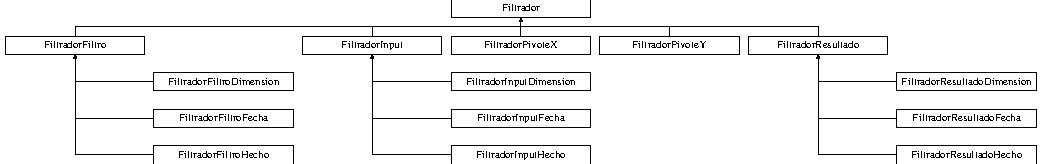
\includegraphics[height=2.209945cm]{classFiltrador}
\end{center}
\end{figure}
\subsection*{\-Métodos públicos}
\begin{DoxyCompactItemize}
\item 
\hyperlink{classFiltrador_a49a38d95ab4cd07bf57a90debe0f9474}{\-Filtrador} (const \-Glib\-::ustring \&filtro)
\item 
virtual \hyperlink{classFiltrador_a85782ed4dd9ca143369f16de7798cb2f}{$\sim$\-Filtrador} ()
\item 
\-Glib\-::ustring \hyperlink{classFiltrador_a652586677727ae345d0f3b1dd6edf7eb}{get\-Filtro} ()
\item 
virtual void \hyperlink{classFiltrador_a5c0739dd669ef0de7f2624c77beb14f0}{filtrar} (\hyperlink{classConsulta}{\-Consulta} \&c)=0
\end{DoxyCompactItemize}
\subsection*{\-Atributos protegidos}
\begin{DoxyCompactItemize}
\item 
\hypertarget{classFiltrador_ac49e35712d9fbbf76930ef14652691f7}{\-Gtk\-::\-H\-Box {\bfseries centrador\-Derecho}}\label{classFiltrador_ac49e35712d9fbbf76930ef14652691f7}

\end{DoxyCompactItemize}


\subsection{\-Descripción detallada}
\-Clase abstracta que representa tanto un constructor de consulta como la vista del mismo. \-Un constructor de consulta es, como se ve en las clases que heredan de esta, un filtro, un input, un resultado y un elemento de \-X e \-Y para la tabla pivot. 

\subsection{\-Documentación del constructor y destructor}
\hypertarget{classFiltrador_a49a38d95ab4cd07bf57a90debe0f9474}{\index{\-Filtrador@{\-Filtrador}!\-Filtrador@{\-Filtrador}}
\index{\-Filtrador@{\-Filtrador}!Filtrador@{\-Filtrador}}
\subsubsection[{\-Filtrador}]{\setlength{\rightskip}{0pt plus 5cm}{\bf \-Filtrador\-::\-Filtrador} (
\begin{DoxyParamCaption}
\item[{const \-Glib\-::ustring \&}]{filtro}
\end{DoxyParamCaption}
)}}\label{classFiltrador_a49a38d95ab4cd07bf57a90debe0f9474}
\-Constructor. 
\begin{DoxyParams}{\-Parámetros}
{\em filtro} & nombre del campo \\
\hline
\end{DoxyParams}
\hypertarget{classFiltrador_a85782ed4dd9ca143369f16de7798cb2f}{\index{\-Filtrador@{\-Filtrador}!$\sim$\-Filtrador@{$\sim$\-Filtrador}}
\index{$\sim$\-Filtrador@{$\sim$\-Filtrador}!Filtrador@{\-Filtrador}}
\subsubsection[{$\sim$\-Filtrador}]{\setlength{\rightskip}{0pt plus 5cm}{\bf \-Filtrador\-::$\sim$\-Filtrador} (
\begin{DoxyParamCaption}
{}
\end{DoxyParamCaption}
)\hspace{0.3cm}{\ttfamily  \mbox{[}virtual\mbox{]}}}}\label{classFiltrador_a85782ed4dd9ca143369f16de7798cb2f}
\-Destructor. 

\subsection{\-Documentación de las funciones miembro}
\hypertarget{classFiltrador_a5c0739dd669ef0de7f2624c77beb14f0}{\index{\-Filtrador@{\-Filtrador}!filtrar@{filtrar}}
\index{filtrar@{filtrar}!Filtrador@{\-Filtrador}}
\subsubsection[{filtrar}]{\setlength{\rightskip}{0pt plus 5cm}virtual void {\bf \-Filtrador\-::filtrar} (
\begin{DoxyParamCaption}
\item[{{\bf \-Consulta} \&}]{c}
\end{DoxyParamCaption}
)\hspace{0.3cm}{\ttfamily  \mbox{[}pure virtual\mbox{]}}}}\label{classFiltrador_a5c0739dd669ef0de7f2624c77beb14f0}
\-Agrega su aporte a la consulta. 
\begin{DoxyParams}{\-Parámetros}
{\em c} & consulta \\
\hline
\end{DoxyParams}


\-Implementado en \hyperlink{classFiltradorFiltroFecha_a77bc9c5c32f89aae6b09b982ff1a1dee}{\-Filtrador\-Filtro\-Fecha}, \hyperlink{classFiltradorInputFecha_a4ca7340057566a1247bc082ba94dad25}{\-Filtrador\-Input\-Fecha}, \hyperlink{classFiltradorInputDimension_a18da290896d3d045a31127f613d12a1c}{\-Filtrador\-Input\-Dimension}, \hyperlink{classFiltradorInputHecho_adaaa9cddc3f560961b108acfc8a002f9}{\-Filtrador\-Input\-Hecho}, \hyperlink{classFiltradorResultadoFecha_a20ed031918bc5f788c8388ab6b26d24c}{\-Filtrador\-Resultado\-Fecha}, \hyperlink{classFiltradorResultadoHecho_adfcbfa61c6efe4003a7b2170ecc44e59}{\-Filtrador\-Resultado\-Hecho}, \hyperlink{classFiltradorFiltroDimension_ab5facda7f5d2953ceb58e96e8be9a2a8}{\-Filtrador\-Filtro\-Dimension}, \hyperlink{classFiltradorPivoteX_aac8f278c7e313efdbaca2aea28730c90}{\-Filtrador\-Pivote\-X}, \hyperlink{classFiltradorPivoteY_a66d31de7db52e27c91073a27fd53b835}{\-Filtrador\-Pivote\-Y}, \hyperlink{classFiltradorResultadoDimension_a60562082b3ad8788d4f912752093eb09}{\-Filtrador\-Resultado\-Dimension} y \hyperlink{classFiltradorFiltroHecho_a87413cf51710bfd0813d0db87c9a1c11}{\-Filtrador\-Filtro\-Hecho}.

\hypertarget{classFiltrador_a652586677727ae345d0f3b1dd6edf7eb}{\index{\-Filtrador@{\-Filtrador}!get\-Filtro@{get\-Filtro}}
\index{get\-Filtro@{get\-Filtro}!Filtrador@{\-Filtrador}}
\subsubsection[{get\-Filtro}]{\setlength{\rightskip}{0pt plus 5cm}\-Glib\-::ustring {\bf \-Filtrador\-::get\-Filtro} (
\begin{DoxyParamCaption}
{}
\end{DoxyParamCaption}
)}}\label{classFiltrador_a652586677727ae345d0f3b1dd6edf7eb}
\-Retorna el nombre del campo. \begin{DoxyReturn}{\-Devuelve}
nombre del campo que afecta este filtrador 
\end{DoxyReturn}


\-La documentación para esta clase fue generada a partir de los siguientes ficheros\-:\begin{DoxyCompactItemize}
\item 
cliente/\-Vista/\-Filtrador.\-h\item 
cliente/\-Vista/\-Filtrador.\-cpp\end{DoxyCompactItemize}

\hypertarget{classFiltradorConfigManager}{\section{\-Referencia de la \-Clase \-Filtrador\-Config\-Manager}
\label{classFiltradorConfigManager}\index{\-Filtrador\-Config\-Manager@{\-Filtrador\-Config\-Manager}}
}


{\ttfamily \#include $<$\-Filtrador\-Config\-Manager.\-h$>$}

\-Diagrama de herencias de \-Filtrador\-Config\-Manager\begin{figure}[H]
\begin{center}
\leavevmode
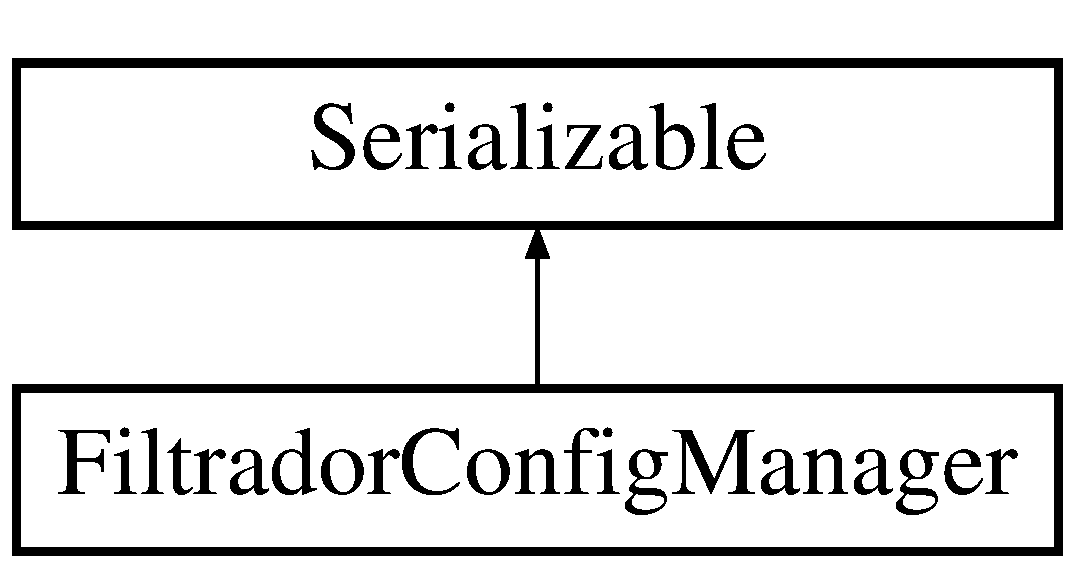
\includegraphics[height=2.000000cm]{classFiltradorConfigManager}
\end{center}
\end{figure}
\subsection*{\-Métodos públicos}
\begin{DoxyCompactItemize}
\item 
\hyperlink{classFiltradorConfigManager_a8e99972eddef35d1950804d6e6a37955}{\-Filtrador\-Config\-Manager} (t\-\_\-\-Filt tipo, const filtradores\-Handlers \&handlers)
\item 
\hyperlink{classFiltradorConfigManager_a14cd6656e2e4ce2a3be00067ea950fcb}{$\sim$\-Filtrador\-Config\-Manager} ()
\item 
\hypertarget{classFiltradorConfigManager_a212aba90eb786881f835ed34b7911aca}{void {\bfseries desconectar} ()}\label{classFiltradorConfigManager_a212aba90eb786881f835ed34b7911aca}

\item 
\hypertarget{classFiltradorConfigManager_aecdfe1a4b7586e9852921867883fbe7d}{void {\bfseries reconectar} ()}\label{classFiltradorConfigManager_aecdfe1a4b7586e9852921867883fbe7d}

\item 
\hypertarget{classFiltradorConfigManager_ae5fd61517aeeed02c65f1e231a1630f6}{void {\bfseries set\-Filtradores\-En} (\hyperlink{classFiltradoresTab}{\-Filtradores\-Tab} $\ast$filt\-Tab)}\label{classFiltradorConfigManager_ae5fd61517aeeed02c65f1e231a1630f6}

\item 
\hypertarget{classFiltradorConfigManager_abc34f32cec4bac96e55a79165a158d27}{void {\bfseries set\-Filtradores\-En} (\hyperlink{classFiltradoresPanel}{\-Filtradores\-Panel} $\ast$filt\-Panel)}\label{classFiltradorConfigManager_abc34f32cec4bac96e55a79165a158d27}

\item 
\hypertarget{classFiltradorConfigManager_ae81242279615ab8eceadf96754492406}{virtual \hyperlink{classTiXmlElement}{\-Nodo\-Xml} {\bfseries serializar} ()}\label{classFiltradorConfigManager_ae81242279615ab8eceadf96754492406}

\item 
\hypertarget{classFiltradorConfigManager_ac24f835cfd67f8c4073d909f42ffac36}{virtual void {\bfseries deserializar} (const \hyperlink{classTiXmlElement}{\-Nodo\-Xml} \&nodo)}\label{classFiltradorConfigManager_ac24f835cfd67f8c4073d909f42ffac36}

\end{DoxyCompactItemize}


\subsection{\-Descripción detallada}
\-Clase encargada de manejar la parte de agregado de filtradores dinámicos por el admin (filtros, inputs, columna \-X e \-Y en tabla pivote, y resultados).

\-Implementa una pequeña factory en base al enum t\-\_\-\-Filt.

\-Está conectado a una señal, en cada uno de los objetos que controla, que informa qué campos están disponibles para ser seleccionados. \-Al recibirla, la difunde por todos sus objetos. 

\subsection{\-Documentación del constructor y destructor}
\hypertarget{classFiltradorConfigManager_a8e99972eddef35d1950804d6e6a37955}{\index{\-Filtrador\-Config\-Manager@{\-Filtrador\-Config\-Manager}!\-Filtrador\-Config\-Manager@{\-Filtrador\-Config\-Manager}}
\index{\-Filtrador\-Config\-Manager@{\-Filtrador\-Config\-Manager}!FiltradorConfigManager@{\-Filtrador\-Config\-Manager}}
\subsubsection[{\-Filtrador\-Config\-Manager}]{\setlength{\rightskip}{0pt plus 5cm}{\bf \-Filtrador\-Config\-Manager\-::\-Filtrador\-Config\-Manager} (
\begin{DoxyParamCaption}
\item[{t\-\_\-\-Filt}]{tipo, }
\item[{const filtradores\-Handlers \&}]{handlers}
\end{DoxyParamCaption}
)}}\label{classFiltradorConfigManager_a8e99972eddef35d1950804d6e6a37955}
\-Constructor. \hypertarget{classFiltradorConfigManager_a14cd6656e2e4ce2a3be00067ea950fcb}{\index{\-Filtrador\-Config\-Manager@{\-Filtrador\-Config\-Manager}!$\sim$\-Filtrador\-Config\-Manager@{$\sim$\-Filtrador\-Config\-Manager}}
\index{$\sim$\-Filtrador\-Config\-Manager@{$\sim$\-Filtrador\-Config\-Manager}!FiltradorConfigManager@{\-Filtrador\-Config\-Manager}}
\subsubsection[{$\sim$\-Filtrador\-Config\-Manager}]{\setlength{\rightskip}{0pt plus 5cm}{\bf \-Filtrador\-Config\-Manager\-::$\sim$\-Filtrador\-Config\-Manager} (
\begin{DoxyParamCaption}
{}
\end{DoxyParamCaption}
)}}\label{classFiltradorConfigManager_a14cd6656e2e4ce2a3be00067ea950fcb}
\-Destructor. 

\-La documentación para esta clase fue generada a partir de los siguientes ficheros\-:\begin{DoxyCompactItemize}
\item 
cliente/\-Modelo/\-Filtrador\-Config\-Manager.\-h\item 
cliente/\-Modelo/\-Filtrador\-Config\-Manager.\-cpp\end{DoxyCompactItemize}

\hypertarget{classFiltradorConfigModelo}{\section{\-Referencia de la \-Clase \-Filtrador\-Config\-Modelo}
\label{classFiltradorConfigModelo}\index{\-Filtrador\-Config\-Modelo@{\-Filtrador\-Config\-Modelo}}
}


{\ttfamily \#include $<$\-Filtrador\-Config\-Modelo.\-h$>$}

\-Diagrama de herencias de \-Filtrador\-Config\-Modelo\begin{figure}[H]
\begin{center}
\leavevmode
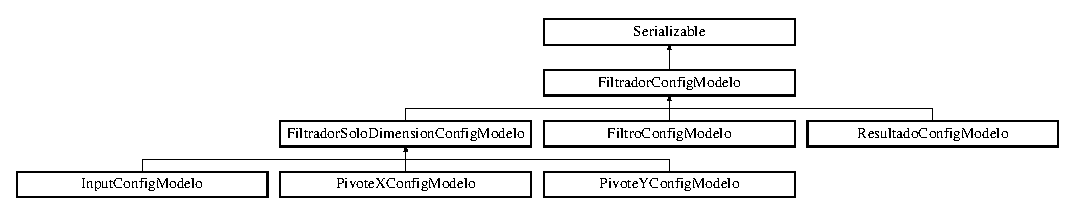
\includegraphics[height=2.434783cm]{classFiltradorConfigModelo}
\end{center}
\end{figure}
\subsection*{\-Métodos públicos}
\begin{DoxyCompactItemize}
\item 
\hyperlink{classFiltradorConfigModelo_aa4bf89d3b9c17421b1885e2666b8d76c}{\-Filtrador\-Config\-Modelo} (unsigned \-I\-D, const std\-::list$<$ std\-::string $>$ \&campos\-Disponibles)
\item 
\hyperlink{classFiltradorConfigModelo_ae3fe5e02af21a1724d2abb940266ac64}{$\sim$\-Filtrador\-Config\-Modelo} ()
\item 
\hypertarget{classFiltradorConfigModelo_abf83fdb10b4c05a534a72dece6526f58}{void {\bfseries set\-Vista} (\-Gtk\-::\-Combo\-Box\-Text $\ast$combo\-Dimension, \-Gtk\-::\-Combo\-Box\-Text $\ast$combo\-Fecha, \-Gtk\-::\-Combo\-Box\-Text $\ast$combo\-Hecho, \-Gtk\-::\-Entry $\ast$entry\-Extra, \-Gtk\-::\-Tool\-Button $\ast$boton\-Eliminar)}\label{classFiltradorConfigModelo_abf83fdb10b4c05a534a72dece6526f58}

\item 
\hypertarget{classFiltradorConfigModelo_abcd792426ccc0f95c6241ddf3fffdcf7}{unsigned {\bfseries get\-I\-D} () const }\label{classFiltradorConfigModelo_abcd792426ccc0f95c6241ddf3fffdcf7}

\item 
void \hyperlink{classFiltradorConfigModelo_a234d1f37a3f7ed8df4a3639dc7eeb319}{actualizar\-Campos} (const \-Glib\-::ustring \&remover, const \-Glib\-::ustring \&agregar)
\item 
\hypertarget{classFiltradorConfigModelo_a388b04e618a004da441f04519d55381f}{sigc\-::signal$<$ void, unsigned $>$ {\bfseries signal\-\_\-delete\-\_\-filtrador} ()}\label{classFiltradorConfigModelo_a388b04e618a004da441f04519d55381f}

\item 
\hypertarget{classFiltradorConfigModelo_a35853241db6782cf6d3172621221e0ad}{sigc\-::signal$<$ void, \*
\-Glib\-::ustring, \-Glib\-::ustring $>$ {\bfseries signal\-\_\-campo\-\_\-changed} ()}\label{classFiltradorConfigModelo_a35853241db6782cf6d3172621221e0ad}

\item 
\hypertarget{classFiltradorConfigModelo_a8dd955d0b124af9bf564b1890e8a3ab1}{virtual void {\bfseries set\-Filtrador\-En} (\hyperlink{classFiltradoresTab}{\-Filtradores\-Tab} $\ast$filt\-Tab)=0}\label{classFiltradorConfigModelo_a8dd955d0b124af9bf564b1890e8a3ab1}

\item 
\hypertarget{classFiltradorConfigModelo_a80cca4f94ccffd75b8022d73e46da642}{virtual void {\bfseries set\-Filtrador\-En} (\hyperlink{classFiltradoresPanel}{\-Filtradores\-Panel} $\ast$filt\-Panel)=0}\label{classFiltradorConfigModelo_a80cca4f94ccffd75b8022d73e46da642}

\item 
\hypertarget{classFiltradorConfigModelo_a0994bf3080dcad82bdbabe433e2a4de0}{virtual \hyperlink{classTiXmlElement}{\-Nodo\-Xml} {\bfseries serializar} ()}\label{classFiltradorConfigModelo_a0994bf3080dcad82bdbabe433e2a4de0}

\item 
\hypertarget{classFiltradorConfigModelo_a91c5fc88daee14e804531af8fc8e2057}{virtual void {\bfseries deserializar} (const \hyperlink{classTiXmlElement}{\-Nodo\-Xml} \&nodo)}\label{classFiltradorConfigModelo_a91c5fc88daee14e804531af8fc8e2057}

\end{DoxyCompactItemize}
\subsection*{\-Métodos protegidos}
\begin{DoxyCompactItemize}
\item 
\hypertarget{classFiltradorConfigModelo_abfc6c03689b768c273f58ab7d0ac4cd5}{virtual void {\bfseries completar\-Atributos} ()=0}\label{classFiltradorConfigModelo_abfc6c03689b768c273f58ab7d0ac4cd5}

\item 
\hypertarget{classFiltradorConfigModelo_abe052870e7ee1ca6222c2cd730281683}{void {\bfseries conectar\-Combo\-Hecho} ()}\label{classFiltradorConfigModelo_abe052870e7ee1ca6222c2cd730281683}

\end{DoxyCompactItemize}
\subsection*{\-Atributos protegidos}
\begin{DoxyCompactItemize}
\item 
\hypertarget{classFiltradorConfigModelo_a43e9f68c76a27aae5ec54eeb1a1666ff}{\-Gtk\-::\-Combo\-Box\-Text $\ast$ {\bfseries combo\-Dimension}}\label{classFiltradorConfigModelo_a43e9f68c76a27aae5ec54eeb1a1666ff}

\item 
\hypertarget{classFiltradorConfigModelo_aba1543a41d1b3c49b3488c58257a32a1}{\-Gtk\-::\-Combo\-Box\-Text $\ast$ {\bfseries combo\-Fecha}}\label{classFiltradorConfigModelo_aba1543a41d1b3c49b3488c58257a32a1}

\item 
\hypertarget{classFiltradorConfigModelo_ad84b08da5792c339d09593272b0389b4}{\-Gtk\-::\-Combo\-Box\-Text $\ast$ {\bfseries combo\-Hecho}}\label{classFiltradorConfigModelo_ad84b08da5792c339d09593272b0389b4}

\item 
\hypertarget{classFiltradorConfigModelo_a323f0f15a5ee911048627126f432e133}{\-Gtk\-::\-Entry $\ast$ {\bfseries entry\-Extra}}\label{classFiltradorConfigModelo_a323f0f15a5ee911048627126f432e133}

\item 
\hypertarget{classFiltradorConfigModelo_ac2aa0b9e2955fbbabc46bbd034974b4a}{\-Glib\-::ustring {\bfseries campo\-Selecc}}\label{classFiltradorConfigModelo_ac2aa0b9e2955fbbabc46bbd034974b4a}

\item 
\hypertarget{classFiltradorConfigModelo_ad5bdaf21bd5e7b23bad35ee52f0a13f7}{\-Glib\-::ustring {\bfseries campo\-Selecc\-Nuevo}}\label{classFiltradorConfigModelo_ad5bdaf21bd5e7b23bad35ee52f0a13f7}

\item 
\hypertarget{classFiltradorConfigModelo_aee91ddf82ded67ca6c5304151d9740a3}{\-Glib\-::ustring {\bfseries \-\_\-valor\-Campo}}\label{classFiltradorConfigModelo_aee91ddf82ded67ca6c5304151d9740a3}

\item 
\hypertarget{classFiltradorConfigModelo_a8bd83eaf50ecbe958c5a1aa5f94dac89}{\-Glib\-::ustring {\bfseries \-\_\-campo\-Aux}}\label{classFiltradorConfigModelo_a8bd83eaf50ecbe958c5a1aa5f94dac89}

\end{DoxyCompactItemize}


\subsection{\-Descripción detallada}
\-Clase base para los modelos que están detrás de las vistas de configuración de filtradores.

\-Es identificable por un número, pero sólo sirve para cuando está en memoria. \-Al persistirse, queda definido por el valor de tres strings\-: -\/el campo de la base de datos por el que filtra -\/un valor auxiliar, que sólo sirve cuando es seleccionado un hecho o fecha, ingresado por combobox -\/otro valor auxiliar, que sólo sirve para \-Filtro y \-Resultado, ingresado por entry

\-Para evitar elegir campos repetidos, cada vez que cambia su selección emite una señal. \-Trabajando en conjunto con \hyperlink{classFiltradorConfigManager}{\-Filtrador\-Config\-Manager}, la señal se difunde y todos sus filtradores hermanos actualizan sus campos disponibles.

\-Un método importante, en paralelo a los \char`\"{}concretar\-Config\char`\"{} de las clases para configurar paneles y tabs, es set\-Filtrador\-En(), sobrecargado para actuar distinto según se agregue a \hyperlink{classFiltradoresTab}{\-Filtradores\-Tab} o \hyperlink{classFiltradoresPanel}{\-Filtradores\-Panel}. \-Lo que hacen es concretar su configuración como filtrador, agregando al conjunto de filtradores. 

\subsection{\-Documentación del constructor y destructor}
\hypertarget{classFiltradorConfigModelo_aa4bf89d3b9c17421b1885e2666b8d76c}{\index{\-Filtrador\-Config\-Modelo@{\-Filtrador\-Config\-Modelo}!\-Filtrador\-Config\-Modelo@{\-Filtrador\-Config\-Modelo}}
\index{\-Filtrador\-Config\-Modelo@{\-Filtrador\-Config\-Modelo}!FiltradorConfigModelo@{\-Filtrador\-Config\-Modelo}}
\subsubsection[{\-Filtrador\-Config\-Modelo}]{\setlength{\rightskip}{0pt plus 5cm}{\bf \-Filtrador\-Config\-Modelo\-::\-Filtrador\-Config\-Modelo} (
\begin{DoxyParamCaption}
\item[{unsigned}]{\-I\-D, }
\item[{const std\-::list$<$ std\-::string $>$ \&}]{campos\-Disponibles}
\end{DoxyParamCaption}
)}}\label{classFiltradorConfigModelo_aa4bf89d3b9c17421b1885e2666b8d76c}
\-Constructor. 
\begin{DoxyParams}{\-Parámetros}
{\em \-I\-D} & identificador de la instancia \\
\hline
{\em campos\-Disponibles} & lista de los campos disponibles, para popular su combobox \\
\hline
\end{DoxyParams}
\hypertarget{classFiltradorConfigModelo_ae3fe5e02af21a1724d2abb940266ac64}{\index{\-Filtrador\-Config\-Modelo@{\-Filtrador\-Config\-Modelo}!$\sim$\-Filtrador\-Config\-Modelo@{$\sim$\-Filtrador\-Config\-Modelo}}
\index{$\sim$\-Filtrador\-Config\-Modelo@{$\sim$\-Filtrador\-Config\-Modelo}!FiltradorConfigModelo@{\-Filtrador\-Config\-Modelo}}
\subsubsection[{$\sim$\-Filtrador\-Config\-Modelo}]{\setlength{\rightskip}{0pt plus 5cm}{\bf \-Filtrador\-Config\-Modelo\-::$\sim$\-Filtrador\-Config\-Modelo} (
\begin{DoxyParamCaption}
{}
\end{DoxyParamCaption}
)}}\label{classFiltradorConfigModelo_ae3fe5e02af21a1724d2abb940266ac64}
\-Destructor. 

\subsection{\-Documentación de las funciones miembro}
\hypertarget{classFiltradorConfigModelo_a234d1f37a3f7ed8df4a3639dc7eeb319}{\index{\-Filtrador\-Config\-Modelo@{\-Filtrador\-Config\-Modelo}!actualizar\-Campos@{actualizar\-Campos}}
\index{actualizar\-Campos@{actualizar\-Campos}!FiltradorConfigModelo@{\-Filtrador\-Config\-Modelo}}
\subsubsection[{actualizar\-Campos}]{\setlength{\rightskip}{0pt plus 5cm}void {\bf \-Filtrador\-Config\-Modelo\-::actualizar\-Campos} (
\begin{DoxyParamCaption}
\item[{const \-Glib\-::ustring \&}]{remover, }
\item[{const \-Glib\-::ustring \&}]{agregar}
\end{DoxyParamCaption}
)}}\label{classFiltradorConfigModelo_a234d1f37a3f7ed8df4a3639dc7eeb319}
\-Actualiza los campos disponibles para elegir. 
\begin{DoxyParams}{\-Parámetros}
{\em remover} & campo a remover de su combobox \\
\hline
{\em agregar} & campo a agregar a su combobox \\
\hline
\end{DoxyParams}


\-La documentación para esta clase fue generada a partir de los siguientes ficheros\-:\begin{DoxyCompactItemize}
\item 
cliente/\-Modelo/\-Filtrador\-Config\-Modelo.\-h\item 
cliente/\-Modelo/\-Filtrador\-Config\-Modelo.\-cpp\end{DoxyCompactItemize}

\hypertarget{classFiltradorConfigVista}{\section{\-Referencia de la \-Clase \-Filtrador\-Config\-Vista}
\label{classFiltradorConfigVista}\index{\-Filtrador\-Config\-Vista@{\-Filtrador\-Config\-Vista}}
}


{\ttfamily \#include $<$\-Filtrador\-Config\-Vista.\-h$>$}

\subsection*{\-Métodos públicos}
\begin{DoxyCompactItemize}
\item 
\hyperlink{classFiltradorConfigVista_a33a2ba1d24a4aa1980b89b0ab3c6e3b4}{\-Filtrador\-Config\-Vista} (\hyperlink{classFiltradorConfigModelo}{\-Filtrador\-Config\-Modelo} $\ast$p\-Modelo)
\item 
\hyperlink{classFiltradorConfigVista_a346460691c2ca8ee496eca47ed52928c}{$\sim$\-Filtrador\-Config\-Vista} ()
\end{DoxyCompactItemize}


\subsection{\-Descripción detallada}
\-Representación visual de la configuración de un filtrador. \-Se construye asociada a un modelo porque a diferencias de las otras vistas, es un modelo por vista.

\-Una vez relaciada al modelo, es controlada desde allí con lo cual, no tiene ninguna otra particularidad. 

\subsection{\-Documentación del constructor y destructor}
\hypertarget{classFiltradorConfigVista_a33a2ba1d24a4aa1980b89b0ab3c6e3b4}{\index{\-Filtrador\-Config\-Vista@{\-Filtrador\-Config\-Vista}!\-Filtrador\-Config\-Vista@{\-Filtrador\-Config\-Vista}}
\index{\-Filtrador\-Config\-Vista@{\-Filtrador\-Config\-Vista}!FiltradorConfigVista@{\-Filtrador\-Config\-Vista}}
\subsubsection[{\-Filtrador\-Config\-Vista}]{\setlength{\rightskip}{0pt plus 5cm}{\bf \-Filtrador\-Config\-Vista\-::\-Filtrador\-Config\-Vista} (
\begin{DoxyParamCaption}
\item[{{\bf \-Filtrador\-Config\-Modelo} $\ast$}]{p\-Modelo}
\end{DoxyParamCaption}
)}}\label{classFiltradorConfigVista_a33a2ba1d24a4aa1980b89b0ab3c6e3b4}
\-Constructor. 
\begin{DoxyParams}{\-Parámetros}
{\em p\-Modelo} & el modelo asociado a esta vista \\
\hline
\end{DoxyParams}
\hypertarget{classFiltradorConfigVista_a346460691c2ca8ee496eca47ed52928c}{\index{\-Filtrador\-Config\-Vista@{\-Filtrador\-Config\-Vista}!$\sim$\-Filtrador\-Config\-Vista@{$\sim$\-Filtrador\-Config\-Vista}}
\index{$\sim$\-Filtrador\-Config\-Vista@{$\sim$\-Filtrador\-Config\-Vista}!FiltradorConfigVista@{\-Filtrador\-Config\-Vista}}
\subsubsection[{$\sim$\-Filtrador\-Config\-Vista}]{\setlength{\rightskip}{0pt plus 5cm}{\bf \-Filtrador\-Config\-Vista\-::$\sim$\-Filtrador\-Config\-Vista} (
\begin{DoxyParamCaption}
{}
\end{DoxyParamCaption}
)}}\label{classFiltradorConfigVista_a346460691c2ca8ee496eca47ed52928c}
\-Destructor. 

\-La documentación para esta clase fue generada a partir de los siguientes ficheros\-:\begin{DoxyCompactItemize}
\item 
cliente/\-Vista/\-Filtrador\-Config\-Vista.\-h\item 
cliente/\-Vista/\-Filtrador\-Config\-Vista.\-cpp\end{DoxyCompactItemize}

\hypertarget{classFiltradores}{\section{\-Referencia de la \-Clase \-Filtradores}
\label{classFiltradores}\index{\-Filtradores@{\-Filtradores}}
}


{\ttfamily \#include $<$\-Filtradores.\-h$>$}

\-Diagrama de herencias de \-Filtradores\begin{figure}[H]
\begin{center}
\leavevmode
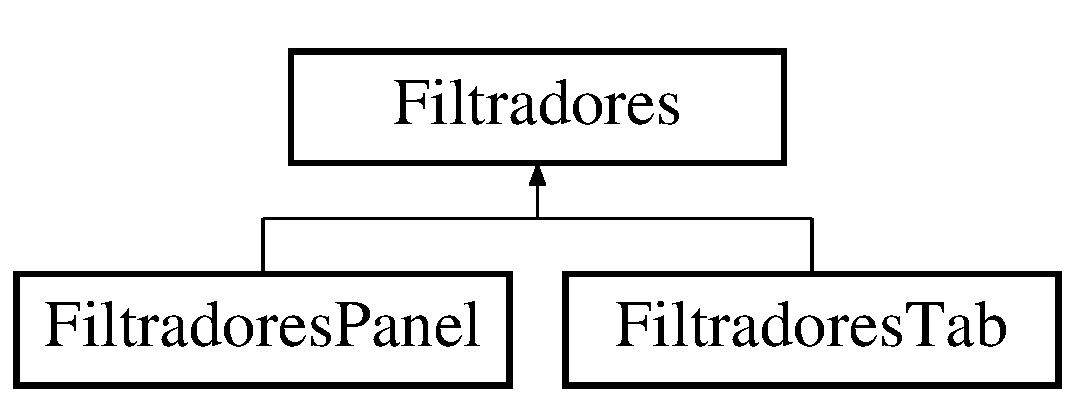
\includegraphics[height=2.000000cm]{classFiltradores}
\end{center}
\end{figure}
\subsection*{\-Métodos públicos}
\begin{DoxyCompactItemize}
\item 
\hyperlink{classFiltradores_a3d450f3b376ff71acb8c06d7be7bf49b}{\-Filtradores} ()
\item 
\hyperlink{classFiltradores_a6d9df7e673dd658d851cb6e809ba472f}{$\sim$\-Filtradores} ()
\item 
\hypertarget{classFiltradores_a62f207dc95b9bfdfd2e4250c82c160f3}{virtual bool {\bfseries puede\-Filtrar} ()}\label{classFiltradores_a62f207dc95b9bfdfd2e4250c82c160f3}

\item 
\hypertarget{classFiltradores_a28e80978bb0e2e03adebae297b76a309}{virtual void {\bfseries filtrar} (\hyperlink{classConsulta}{\-Consulta} \&c)}\label{classFiltradores_a28e80978bb0e2e03adebae297b76a309}

\item 
\hypertarget{classFiltradores_a84dc1b94f28a2965e90b36bc149ab164}{virtual void {\bfseries agregar\-Entrada} (const std\-::string \&entrada)=0}\label{classFiltradores_a84dc1b94f28a2965e90b36bc149ab164}

\item 
\hypertarget{classFiltradores_ad302fc3bea625acdd3f623afbcc8a030}{bool {\bfseries tiene\-Filtros\-Navegables} ()}\label{classFiltradores_ad302fc3bea625acdd3f623afbcc8a030}

\item 
\hypertarget{classFiltradores_a5d4e09183a8858e6fd410202cbf9ace4}{bool {\bfseries tiene\-Filtros\-Consultantes} ()}\label{classFiltradores_a5d4e09183a8858e6fd410202cbf9ace4}

\item 
\hypertarget{classFiltradores_a538fe2160d8d3037563603c47e9566f2}{\hyperlink{classFiltradorInput}{\-Filtrador\-Input} $\ast$ {\bfseries get\-Filtro\-Navegable} ()}\label{classFiltradores_a538fe2160d8d3037563603c47e9566f2}

\item 
\hypertarget{classFiltradores_a6d64cad1b899951c50ac42cbaf49921f}{\hyperlink{classFiltradorInputDimension}{\-Filtrador\-Input\-Dimension} $\ast$ {\bfseries get\-Filtro\-Consultante} ()}\label{classFiltradores_a6d64cad1b899951c50ac42cbaf49921f}

\end{DoxyCompactItemize}
\subsection*{\-Métodos protegidos}
\begin{DoxyCompactItemize}
\item 
void \hyperlink{classFiltradores_a53e6d4e610239dc8890853ac0ac647a6}{on\-\_\-input\-\_\-esta\-\_\-disponible} (bool estado)
\end{DoxyCompactItemize}
\subsection*{\-Atributos protegidos}
\begin{DoxyCompactItemize}
\item 
\hypertarget{classFiltradores_aca46b72d23d8c16e708768340994eef6}{std\-::list$<$ \hyperlink{classFiltrador}{\-Filtrador} $\ast$ $>$ {\bfseries filtradores}}\label{classFiltradores_aca46b72d23d8c16e708768340994eef6}

\item 
\hypertarget{classFiltradores_ad8e0a2aecedd410cf8fc268a87f39135}{std\-::queue$<$ \hyperlink{classFiltradorInput}{\-Filtrador\-Input} $\ast$ $>$ {\bfseries filtros\-Navegables}}\label{classFiltradores_ad8e0a2aecedd410cf8fc268a87f39135}

\item 
\hypertarget{classFiltradores_aa97b49681afb1fa7a0a03d0ebb11db1f}{std\-::queue\*
$<$ \hyperlink{classFiltradorInputDimension}{\-Filtrador\-Input\-Dimension} $\ast$ $>$ {\bfseries filtros\-Consultantes}}\label{classFiltradores_aa97b49681afb1fa7a0a03d0ebb11db1f}

\item 
\hypertarget{classFiltradores_add3494980d7aafcf16e2c77cfd7bce10}{unsigned {\bfseries cant\-\_\-inputs}}\label{classFiltradores_add3494980d7aafcf16e2c77cfd7bce10}

\item 
\hypertarget{classFiltradores_a007d812879b019b9299465d02d848cfd}{unsigned {\bfseries inputs\-Disponibles}}\label{classFiltradores_a007d812879b019b9299465d02d848cfd}

\item 
\hypertarget{classFiltradores_a8d54b2ddb1d763c323c77ce53a1cacb6}{bool {\bfseries \-\_\-puede\-Filtrar}}\label{classFiltradores_a8d54b2ddb1d763c323c77ce53a1cacb6}

\end{DoxyCompactItemize}


\subsection{\-Descripción detallada}
\-Clase abstracta que representa tanto un conjunto de filtradores como la vista del conjunto. \-Cada filtrador se dispone uno abajo del otro. 

\subsection{\-Documentación del constructor y destructor}
\hypertarget{classFiltradores_a3d450f3b376ff71acb8c06d7be7bf49b}{\index{\-Filtradores@{\-Filtradores}!\-Filtradores@{\-Filtradores}}
\index{\-Filtradores@{\-Filtradores}!Filtradores@{\-Filtradores}}
\subsubsection[{\-Filtradores}]{\setlength{\rightskip}{0pt plus 5cm}{\bf \-Filtradores\-::\-Filtradores} (
\begin{DoxyParamCaption}
{}
\end{DoxyParamCaption}
)}}\label{classFiltradores_a3d450f3b376ff71acb8c06d7be7bf49b}
\-Constructor. \hypertarget{classFiltradores_a6d9df7e673dd658d851cb6e809ba472f}{\index{\-Filtradores@{\-Filtradores}!$\sim$\-Filtradores@{$\sim$\-Filtradores}}
\index{$\sim$\-Filtradores@{$\sim$\-Filtradores}!Filtradores@{\-Filtradores}}
\subsubsection[{$\sim$\-Filtradores}]{\setlength{\rightskip}{0pt plus 5cm}{\bf \-Filtradores\-::$\sim$\-Filtradores} (
\begin{DoxyParamCaption}
{}
\end{DoxyParamCaption}
)}}\label{classFiltradores_a6d9df7e673dd658d851cb6e809ba472f}
\-Destructor. 

\subsection{\-Documentación de las funciones miembro}
\hypertarget{classFiltradores_a53e6d4e610239dc8890853ac0ac647a6}{\index{\-Filtradores@{\-Filtradores}!on\-\_\-input\-\_\-esta\-\_\-disponible@{on\-\_\-input\-\_\-esta\-\_\-disponible}}
\index{on\-\_\-input\-\_\-esta\-\_\-disponible@{on\-\_\-input\-\_\-esta\-\_\-disponible}!Filtradores@{\-Filtradores}}
\subsubsection[{on\-\_\-input\-\_\-esta\-\_\-disponible}]{\setlength{\rightskip}{0pt plus 5cm}void {\bf \-Filtradores\-::on\-\_\-input\-\_\-esta\-\_\-disponible} (
\begin{DoxyParamCaption}
\item[{bool}]{estado}
\end{DoxyParamCaption}
)\hspace{0.3cm}{\ttfamily  \mbox{[}protected\mbox{]}}}}\label{classFiltradores_a53e6d4e610239dc8890853ac0ac647a6}
\-Signal handler para la señal \-Filtrador\-Input\-::\-\_\-signal\-\_\-input\-\_\-disponible.

\-Aumenta o disminuye la cantidad de inputs disponibles, según sea true o false el parámetro. \-Si todos los inputs están disponibles entonces puede filtrar una consulta. 
\begin{DoxyParams}{\-Parámetros}
{\em estado} & estado de la disponibilidad del input \\
\hline
\end{DoxyParams}


\-La documentación para esta clase fue generada a partir de los siguientes ficheros\-:\begin{DoxyCompactItemize}
\item 
cliente/\-Vista/\-Filtradores.\-h\item 
cliente/\-Vista/\-Filtradores.\-cpp\end{DoxyCompactItemize}

\hypertarget{classFiltradoresPanel}{\section{\-Referencia de la \-Clase \-Filtradores\-Panel}
\label{classFiltradoresPanel}\index{\-Filtradores\-Panel@{\-Filtradores\-Panel}}
}


{\ttfamily \#include $<$\-Filtradores\-Panel.\-h$>$}

\-Diagrama de herencias de \-Filtradores\-Panel\begin{figure}[H]
\begin{center}
\leavevmode
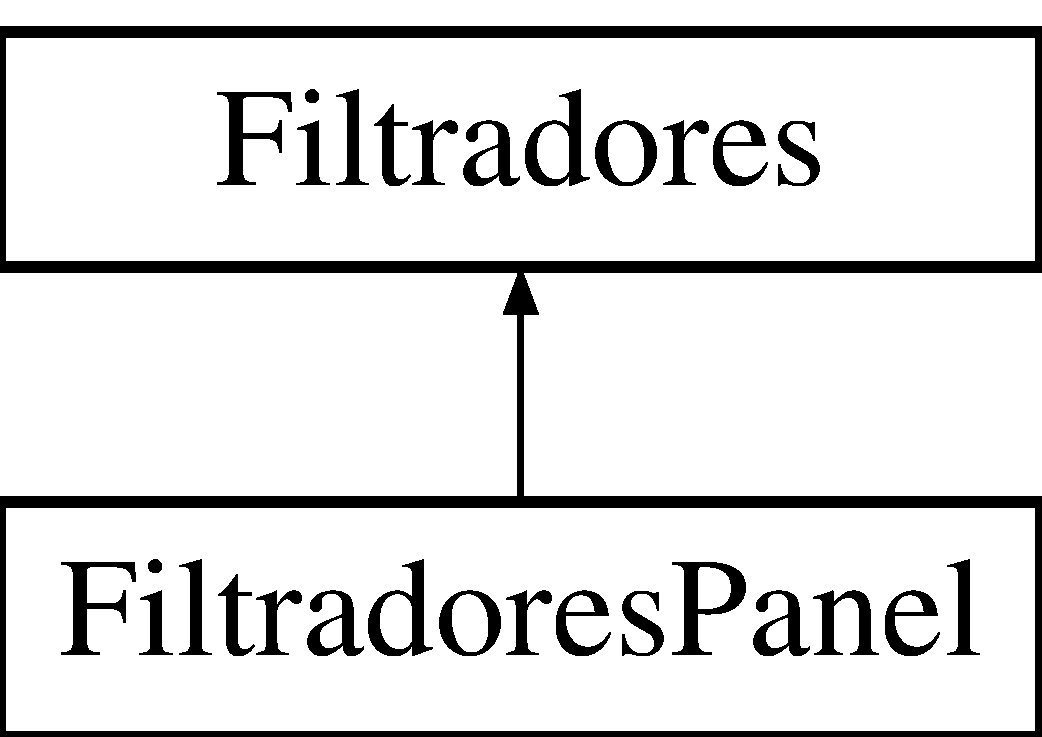
\includegraphics[height=2.000000cm]{classFiltradoresPanel}
\end{center}
\end{figure}
\subsection*{\-Métodos públicos}
\begin{DoxyCompactItemize}
\item 
\hyperlink{classFiltradoresPanel_adb3759f9adfd87c8f784ec2733ff22f4}{\-Filtradores\-Panel} (\hyperlink{classFiltradoresTab}{\-Filtradores\-Tab} \&filt\-Tab)
\item 
\hyperlink{classFiltradoresPanel_a8c6641e68a9fba171b0d93f5e383e2c7}{$\sim$\-Filtradores\-Panel} ()
\item 
\hypertarget{classFiltradoresPanel_ac557ec32085b68c5c9a618411cf57b32}{bool {\bfseries puede\-Filtrar} ()}\label{classFiltradoresPanel_ac557ec32085b68c5c9a618411cf57b32}

\item 
\hypertarget{classFiltradoresPanel_a472ba816f43c83059e382a1972d26241}{void {\bfseries filtrar} (\hyperlink{classConsulta}{\-Consulta} \&c)}\label{classFiltradoresPanel_a472ba816f43c83059e382a1972d26241}

\item 
\hypertarget{classFiltradoresPanel_ace569cbd25135b114493adba3c899dce}{void \hyperlink{classFiltradoresPanel_ace569cbd25135b114493adba3c899dce}{agregar\-Filtro} (const std\-::string \&dimension, const std\-::string \&valor)}\label{classFiltradoresPanel_ace569cbd25135b114493adba3c899dce}

\begin{DoxyCompactList}\small\item\em este método no verifica que el filtro sea dimensión \end{DoxyCompactList}\item 
\hypertarget{classFiltradoresPanel_a3104a1deb1ecddb9a994843ac3608c2a}{void {\bfseries agregar\-Filtro} (const std\-::string \&filtro, const std\-::string \&valor\-Combo, const std\-::string \&valor\-Entrada)}\label{classFiltradoresPanel_a3104a1deb1ecddb9a994843ac3608c2a}

\item 
\hypertarget{classFiltradoresPanel_a52958ba84e6f4efc5d38c3aece3aa9e0}{void {\bfseries agregar\-Entrada} (const std\-::string \&entrada)}\label{classFiltradoresPanel_a52958ba84e6f4efc5d38c3aece3aa9e0}

\item 
\hypertarget{classFiltradoresPanel_ae849890d22b0d32762b27fc4af325f52}{void {\bfseries agregar\-X\-Tabla\-P} (const std\-::string \&valor)}\label{classFiltradoresPanel_ae849890d22b0d32762b27fc4af325f52}

\item 
\hypertarget{classFiltradoresPanel_aaed9cc5c1056264d2f422ff78c2ca545}{void {\bfseries agregar\-Y\-Tabla\-P} (const std\-::string \&valor)}\label{classFiltradoresPanel_aaed9cc5c1056264d2f422ff78c2ca545}

\item 
void \hyperlink{classFiltradoresPanel_aadf1d546161094234541c02f15eaea00}{agregar\-Resultado} (const std\-::string \&dimension)
\item 
\hypertarget{classFiltradoresPanel_ad2fdf19683ace05463081371204ea092}{void {\bfseries agregar\-Resultado} (const std\-::string \&fecha, const std\-::string \&valor\-Combo, const std\-::string \&valor\-Entrada)}\label{classFiltradoresPanel_ad2fdf19683ace05463081371204ea092}

\item 
\hypertarget{classFiltradoresPanel_a55f2a7dde1e8b0d3d2b12a0e810f4a38}{void {\bfseries agregar\-Resultado} (const std\-::string \&hecho, const std\-::string \&agregacion)}\label{classFiltradoresPanel_a55f2a7dde1e8b0d3d2b12a0e810f4a38}

\item 
\hypertarget{classFiltradoresPanel_afc27cd818da0c0bef5c8668df186c240}{sigc\-::signal$<$ void $>$ {\bfseries signal\-\_\-navegabilidad} ()}\label{classFiltradoresPanel_afc27cd818da0c0bef5c8668df186c240}

\end{DoxyCompactItemize}


\subsection{\-Descripción detallada}
\-Implementación concreta de un conjunto de filtradores, el de los paneles. \-Admiten todos los filtradores existentes, aunque cuando se agrega uno para \-X o \-Y de tabla pivote, la consulta al ser filtrada quedará definida como dicha tabla. 

\subsection{\-Documentación del constructor y destructor}
\hypertarget{classFiltradoresPanel_adb3759f9adfd87c8f784ec2733ff22f4}{\index{\-Filtradores\-Panel@{\-Filtradores\-Panel}!\-Filtradores\-Panel@{\-Filtradores\-Panel}}
\index{\-Filtradores\-Panel@{\-Filtradores\-Panel}!FiltradoresPanel@{\-Filtradores\-Panel}}
\subsubsection[{\-Filtradores\-Panel}]{\setlength{\rightskip}{0pt plus 5cm}{\bf \-Filtradores\-Panel\-::\-Filtradores\-Panel} (
\begin{DoxyParamCaption}
\item[{{\bf \-Filtradores\-Tab} \&}]{filt\-Tab}
\end{DoxyParamCaption}
)}}\label{classFiltradoresPanel_adb3759f9adfd87c8f784ec2733ff22f4}
\-Constructor. 
\begin{DoxyParams}{\-Parámetros}
{\em filt\-Tab} & referencia a los filtradores de la tab \\
\hline
\end{DoxyParams}
\hypertarget{classFiltradoresPanel_a8c6641e68a9fba171b0d93f5e383e2c7}{\index{\-Filtradores\-Panel@{\-Filtradores\-Panel}!$\sim$\-Filtradores\-Panel@{$\sim$\-Filtradores\-Panel}}
\index{$\sim$\-Filtradores\-Panel@{$\sim$\-Filtradores\-Panel}!FiltradoresPanel@{\-Filtradores\-Panel}}
\subsubsection[{$\sim$\-Filtradores\-Panel}]{\setlength{\rightskip}{0pt plus 5cm}{\bf \-Filtradores\-Panel\-::$\sim$\-Filtradores\-Panel} (
\begin{DoxyParamCaption}
{}
\end{DoxyParamCaption}
)}}\label{classFiltradoresPanel_a8c6641e68a9fba171b0d93f5e383e2c7}
\-Destructor. 

\subsection{\-Documentación de las funciones miembro}
\hypertarget{classFiltradoresPanel_aadf1d546161094234541c02f15eaea00}{\index{\-Filtradores\-Panel@{\-Filtradores\-Panel}!agregar\-Resultado@{agregar\-Resultado}}
\index{agregar\-Resultado@{agregar\-Resultado}!FiltradoresPanel@{\-Filtradores\-Panel}}
\subsubsection[{agregar\-Resultado}]{\setlength{\rightskip}{0pt plus 5cm}void {\bf \-Filtradores\-Panel\-::agregar\-Resultado} (
\begin{DoxyParamCaption}
\item[{const std\-::string \&}]{dimension}
\end{DoxyParamCaption}
)}}\label{classFiltradoresPanel_aadf1d546161094234541c02f15eaea00}
estos tres métodos no verifican que el primer parámetro sea dimensión, fecha o hecho 

\-La documentación para esta clase fue generada a partir de los siguientes ficheros\-:\begin{DoxyCompactItemize}
\item 
cliente/\-Vista/\-Filtradores\-Panel.\-h\item 
cliente/\-Vista/\-Filtradores\-Panel.\-cpp\end{DoxyCompactItemize}

\hypertarget{classFiltradoresTab}{\section{\-Referencia de la \-Clase \-Filtradores\-Tab}
\label{classFiltradoresTab}\index{\-Filtradores\-Tab@{\-Filtradores\-Tab}}
}


{\ttfamily \#include $<$\-Filtradores\-Tab.\-h$>$}

\-Diagrama de herencias de \-Filtradores\-Tab\begin{figure}[H]
\begin{center}
\leavevmode
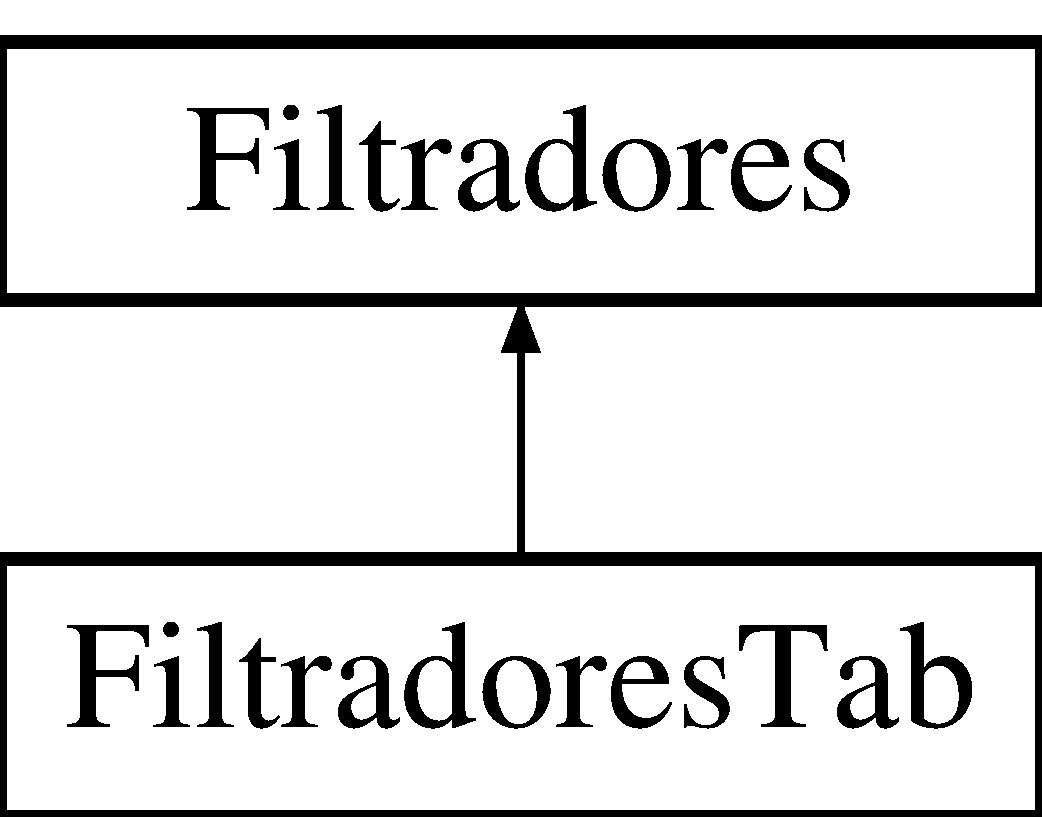
\includegraphics[height=2.000000cm]{classFiltradoresTab}
\end{center}
\end{figure}
\subsection*{\-Métodos públicos}
\begin{DoxyCompactItemize}
\item 
\hyperlink{classFiltradoresTab_addce817d4d87056260859935f50b1c05}{\-Filtradores\-Tab} ()
\item 
\hyperlink{classFiltradoresTab_a37bb0ad95be5e9f00e9d3f012ce3c5ee}{$\sim$\-Filtradores\-Tab} ()
\item 
\hypertarget{classFiltradoresTab_a3263fde5111452e4943b9611fdd87939}{void {\bfseries agregar\-Entrada} (const std\-::string \&entrada)}\label{classFiltradoresTab_a3263fde5111452e4943b9611fdd87939}

\end{DoxyCompactItemize}


\subsection{\-Descripción detallada}
\-Implementación concreta de un conjunto de filtradores, el de las tabs. \-Sólo admiten inputs, y se aplican a todo panel dentro de la pestaña. 

\subsection{\-Documentación del constructor y destructor}
\hypertarget{classFiltradoresTab_addce817d4d87056260859935f50b1c05}{\index{\-Filtradores\-Tab@{\-Filtradores\-Tab}!\-Filtradores\-Tab@{\-Filtradores\-Tab}}
\index{\-Filtradores\-Tab@{\-Filtradores\-Tab}!FiltradoresTab@{\-Filtradores\-Tab}}
\subsubsection[{\-Filtradores\-Tab}]{\setlength{\rightskip}{0pt plus 5cm}{\bf \-Filtradores\-Tab\-::\-Filtradores\-Tab} (
\begin{DoxyParamCaption}
{}
\end{DoxyParamCaption}
)}}\label{classFiltradoresTab_addce817d4d87056260859935f50b1c05}
\-Constructor. \hypertarget{classFiltradoresTab_a37bb0ad95be5e9f00e9d3f012ce3c5ee}{\index{\-Filtradores\-Tab@{\-Filtradores\-Tab}!$\sim$\-Filtradores\-Tab@{$\sim$\-Filtradores\-Tab}}
\index{$\sim$\-Filtradores\-Tab@{$\sim$\-Filtradores\-Tab}!FiltradoresTab@{\-Filtradores\-Tab}}
\subsubsection[{$\sim$\-Filtradores\-Tab}]{\setlength{\rightskip}{0pt plus 5cm}{\bf \-Filtradores\-Tab\-::$\sim$\-Filtradores\-Tab} (
\begin{DoxyParamCaption}
{}
\end{DoxyParamCaption}
)}}\label{classFiltradoresTab_a37bb0ad95be5e9f00e9d3f012ce3c5ee}
\-Destructor. 

\-La documentación para esta clase fue generada a partir de los siguientes ficheros\-:\begin{DoxyCompactItemize}
\item 
cliente/\-Vista/\-Filtradores\-Tab.\-h\item 
cliente/\-Vista/\-Filtradores\-Tab.\-cpp\end{DoxyCompactItemize}

\hypertarget{classFiltradorFiltro}{\section{\-Referencia de la \-Clase \-Filtrador\-Filtro}
\label{classFiltradorFiltro}\index{\-Filtrador\-Filtro@{\-Filtrador\-Filtro}}
}


{\ttfamily \#include $<$\-Filtrador\-Filtro.\-h$>$}

\-Diagrama de herencias de \-Filtrador\-Filtro\begin{figure}[H]
\begin{center}
\leavevmode
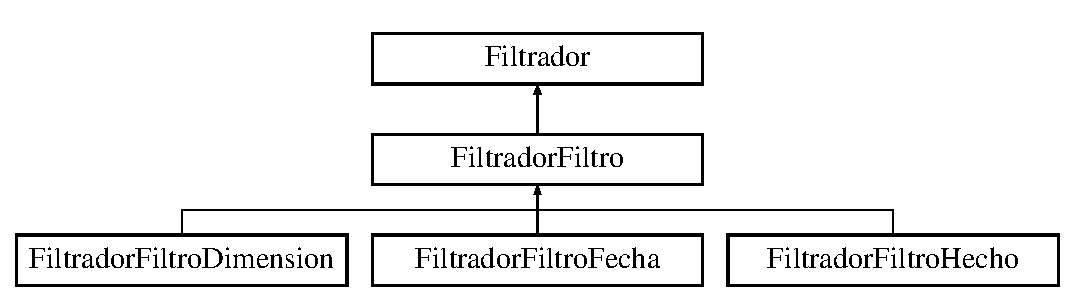
\includegraphics[height=3.000000cm]{classFiltradorFiltro}
\end{center}
\end{figure}
\subsection*{\-Métodos públicos}
\begin{DoxyCompactItemize}
\item 
\hyperlink{classFiltradorFiltro_ae351a76bc1f25cd13690849099acd5b8}{\-Filtrador\-Filtro} (const \-Glib\-::ustring \&filtro, const \-Glib\-::ustring \&valor)
\item 
virtual \hyperlink{classFiltradorFiltro_a2711e32e97e506736fbf292e295008c0}{$\sim$\-Filtrador\-Filtro} ()
\end{DoxyCompactItemize}
\subsection*{\-Métodos protegidos}
\begin{DoxyCompactItemize}
\item 
\hypertarget{classFiltradorFiltro_a19c28369cdcaa75763ace7d5d8437f35}{void {\bfseries set\-Valor} (const \-Glib\-::ustring \&valor)}\label{classFiltradorFiltro_a19c28369cdcaa75763ace7d5d8437f35}

\item 
\hypertarget{classFiltradorFiltro_a05e66a888382870d8e5a478c9ff64160}{\-Glib\-::ustring {\bfseries get\-Valor} ()}\label{classFiltradorFiltro_a05e66a888382870d8e5a478c9ff64160}

\end{DoxyCompactItemize}


\subsection{\-Descripción detallada}
\hyperlink{classFiltrador}{\-Filtrador} concretado en un filtro. \-Como todavía varía según se filtre por hecho, dimensión o fecha, sigue siendo una clase abstracta. 

\subsection{\-Documentación del constructor y destructor}
\hypertarget{classFiltradorFiltro_ae351a76bc1f25cd13690849099acd5b8}{\index{\-Filtrador\-Filtro@{\-Filtrador\-Filtro}!\-Filtrador\-Filtro@{\-Filtrador\-Filtro}}
\index{\-Filtrador\-Filtro@{\-Filtrador\-Filtro}!FiltradorFiltro@{\-Filtrador\-Filtro}}
\subsubsection[{\-Filtrador\-Filtro}]{\setlength{\rightskip}{0pt plus 5cm}{\bf \-Filtrador\-Filtro\-::\-Filtrador\-Filtro} (
\begin{DoxyParamCaption}
\item[{const \-Glib\-::ustring \&}]{filtro, }
\item[{const \-Glib\-::ustring \&}]{valor}
\end{DoxyParamCaption}
)}}\label{classFiltradorFiltro_ae351a76bc1f25cd13690849099acd5b8}
\-Constructor. \hypertarget{classFiltradorFiltro_a2711e32e97e506736fbf292e295008c0}{\index{\-Filtrador\-Filtro@{\-Filtrador\-Filtro}!$\sim$\-Filtrador\-Filtro@{$\sim$\-Filtrador\-Filtro}}
\index{$\sim$\-Filtrador\-Filtro@{$\sim$\-Filtrador\-Filtro}!FiltradorFiltro@{\-Filtrador\-Filtro}}
\subsubsection[{$\sim$\-Filtrador\-Filtro}]{\setlength{\rightskip}{0pt plus 5cm}{\bf \-Filtrador\-Filtro\-::$\sim$\-Filtrador\-Filtro} (
\begin{DoxyParamCaption}
{}
\end{DoxyParamCaption}
)\hspace{0.3cm}{\ttfamily  \mbox{[}virtual\mbox{]}}}}\label{classFiltradorFiltro_a2711e32e97e506736fbf292e295008c0}
\-Destructor. 

\-La documentación para esta clase fue generada a partir de los siguientes ficheros\-:\begin{DoxyCompactItemize}
\item 
cliente/\-Vista/\-Filtrador\-Filtro.\-h\item 
cliente/\-Vista/\-Filtrador\-Filtro.\-cpp\end{DoxyCompactItemize}

\hypertarget{classFiltradorFiltroDimension}{\section{\-Referencia de la \-Clase \-Filtrador\-Filtro\-Dimension}
\label{classFiltradorFiltroDimension}\index{\-Filtrador\-Filtro\-Dimension@{\-Filtrador\-Filtro\-Dimension}}
}


{\ttfamily \#include $<$\-Filtrador\-Filtro\-Dimension.\-h$>$}

\-Diagrama de herencias de \-Filtrador\-Filtro\-Dimension\begin{figure}[H]
\begin{center}
\leavevmode
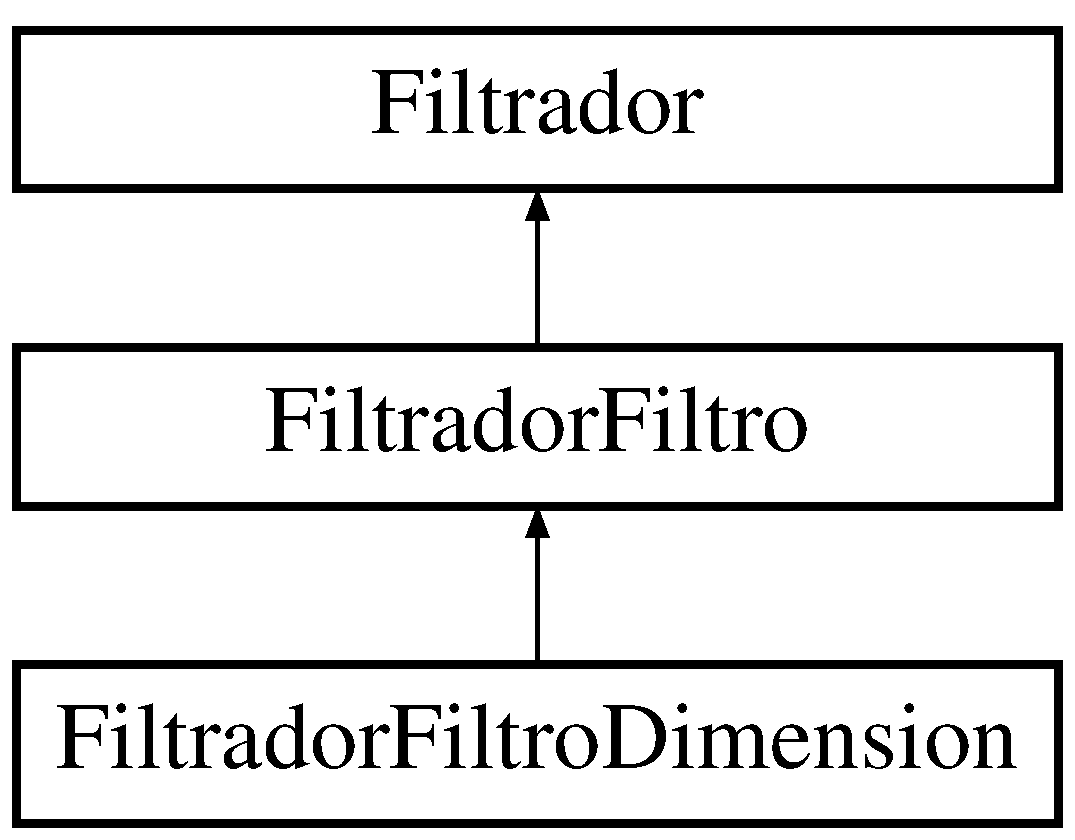
\includegraphics[height=3.000000cm]{classFiltradorFiltroDimension}
\end{center}
\end{figure}
\subsection*{\-Métodos públicos}
\begin{DoxyCompactItemize}
\item 
\hyperlink{classFiltradorFiltroDimension_ae4ed8edd4388b199e5d5bbfedd072bde}{\-Filtrador\-Filtro\-Dimension} (const \-Glib\-::ustring \&filtro, const \-Glib\-::ustring \&valor)
\item 
\hyperlink{classFiltradorFiltroDimension_a93fe672b572712527a550f15fa43edf3}{$\sim$\-Filtrador\-Filtro\-Dimension} ()
\item 
void \hyperlink{classFiltradorFiltroDimension_ab5facda7f5d2953ceb58e96e8be9a2a8}{filtrar} (\hyperlink{classConsulta}{\-Consulta} \&c)
\end{DoxyCompactItemize}


\subsection{\-Descripción detallada}
\-Filtro de comportamiento \char`\"{}básico\char`\"{}, es decir, no es hecho ni fecha. 

\subsection{\-Documentación del constructor y destructor}
\hypertarget{classFiltradorFiltroDimension_ae4ed8edd4388b199e5d5bbfedd072bde}{\index{\-Filtrador\-Filtro\-Dimension@{\-Filtrador\-Filtro\-Dimension}!\-Filtrador\-Filtro\-Dimension@{\-Filtrador\-Filtro\-Dimension}}
\index{\-Filtrador\-Filtro\-Dimension@{\-Filtrador\-Filtro\-Dimension}!FiltradorFiltroDimension@{\-Filtrador\-Filtro\-Dimension}}
\subsubsection[{\-Filtrador\-Filtro\-Dimension}]{\setlength{\rightskip}{0pt plus 5cm}{\bf \-Filtrador\-Filtro\-Dimension\-::\-Filtrador\-Filtro\-Dimension} (
\begin{DoxyParamCaption}
\item[{const \-Glib\-::ustring \&}]{filtro, }
\item[{const \-Glib\-::ustring \&}]{valor}
\end{DoxyParamCaption}
)}}\label{classFiltradorFiltroDimension_ae4ed8edd4388b199e5d5bbfedd072bde}
\-Constructor. \hypertarget{classFiltradorFiltroDimension_a93fe672b572712527a550f15fa43edf3}{\index{\-Filtrador\-Filtro\-Dimension@{\-Filtrador\-Filtro\-Dimension}!$\sim$\-Filtrador\-Filtro\-Dimension@{$\sim$\-Filtrador\-Filtro\-Dimension}}
\index{$\sim$\-Filtrador\-Filtro\-Dimension@{$\sim$\-Filtrador\-Filtro\-Dimension}!FiltradorFiltroDimension@{\-Filtrador\-Filtro\-Dimension}}
\subsubsection[{$\sim$\-Filtrador\-Filtro\-Dimension}]{\setlength{\rightskip}{0pt plus 5cm}{\bf \-Filtrador\-Filtro\-Dimension\-::$\sim$\-Filtrador\-Filtro\-Dimension} (
\begin{DoxyParamCaption}
{}
\end{DoxyParamCaption}
)}}\label{classFiltradorFiltroDimension_a93fe672b572712527a550f15fa43edf3}
\-Destructor. 

\subsection{\-Documentación de las funciones miembro}
\hypertarget{classFiltradorFiltroDimension_ab5facda7f5d2953ceb58e96e8be9a2a8}{\index{\-Filtrador\-Filtro\-Dimension@{\-Filtrador\-Filtro\-Dimension}!filtrar@{filtrar}}
\index{filtrar@{filtrar}!FiltradorFiltroDimension@{\-Filtrador\-Filtro\-Dimension}}
\subsubsection[{filtrar}]{\setlength{\rightskip}{0pt plus 5cm}void {\bf \-Filtrador\-Filtro\-Dimension\-::filtrar} (
\begin{DoxyParamCaption}
\item[{{\bf \-Consulta} \&}]{c}
\end{DoxyParamCaption}
)\hspace{0.3cm}{\ttfamily  \mbox{[}virtual\mbox{]}}}}\label{classFiltradorFiltroDimension_ab5facda7f5d2953ceb58e96e8be9a2a8}
\-Agrega el filtro a la consulta. 
\begin{DoxyParams}{\-Parámetros}
{\em c} & consulta \\
\hline
\end{DoxyParams}


\-Implementa \hyperlink{classFiltrador_a5c0739dd669ef0de7f2624c77beb14f0}{\-Filtrador}.



\-La documentación para esta clase fue generada a partir de los siguientes ficheros\-:\begin{DoxyCompactItemize}
\item 
cliente/\-Vista/\-Filtrador\-Filtro\-Dimension.\-h\item 
cliente/\-Vista/\-Filtrador\-Filtro\-Dimension.\-cpp\end{DoxyCompactItemize}

\hypertarget{classFiltradorFiltroFecha}{\section{\-Referencia de la \-Clase \-Filtrador\-Filtro\-Fecha}
\label{classFiltradorFiltroFecha}\index{\-Filtrador\-Filtro\-Fecha@{\-Filtrador\-Filtro\-Fecha}}
}


{\ttfamily \#include $<$\-Filtrador\-Filtro\-Fecha.\-h$>$}

\-Diagrama de herencias de \-Filtrador\-Filtro\-Fecha\begin{figure}[H]
\begin{center}
\leavevmode
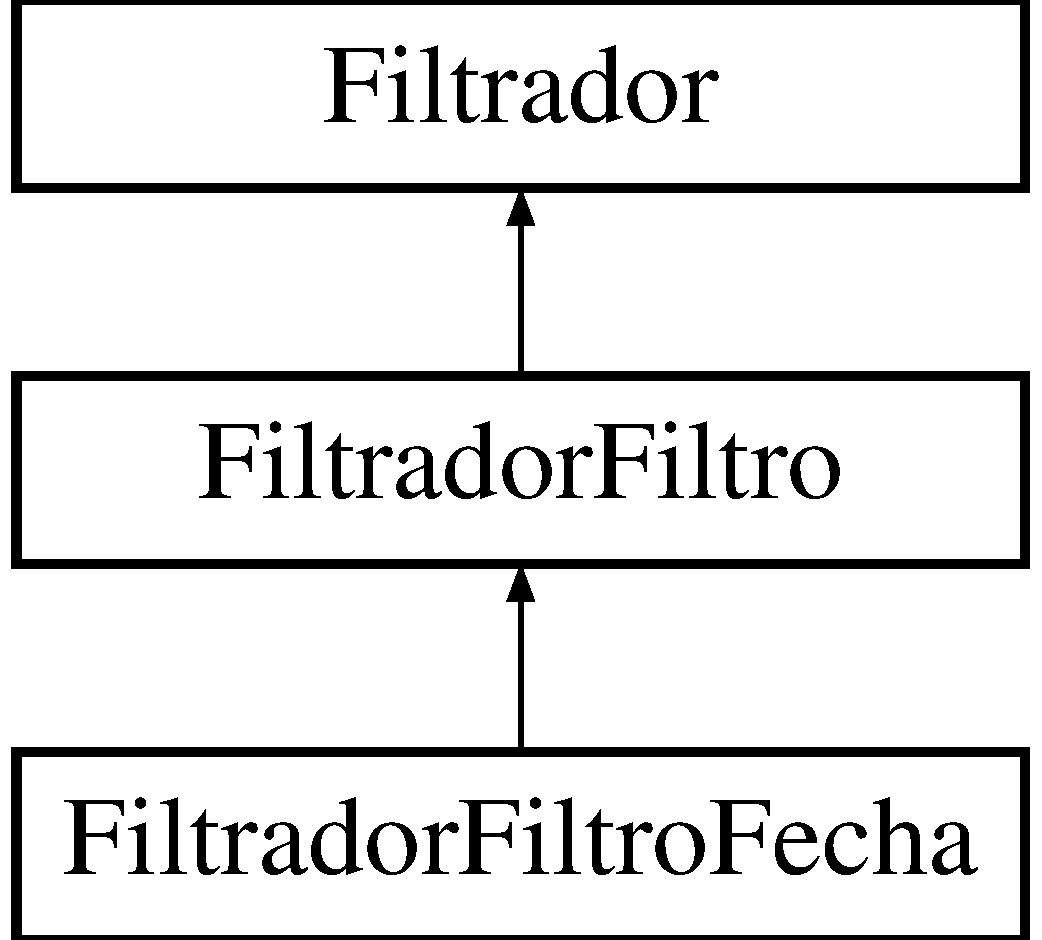
\includegraphics[height=3.000000cm]{classFiltradorFiltroFecha}
\end{center}
\end{figure}
\subsection*{\-Métodos públicos}
\begin{DoxyCompactItemize}
\item 
\hyperlink{classFiltradorFiltroFecha_a6545fb5ca381d50aabc6cb2f8ff1d681}{\-Filtrador\-Filtro\-Fecha} (const \-Glib\-::ustring \&fecha, const \-Glib\-::ustring \&valor\-Combo, const std\-::string \&valor\-Entrada)
\item 
\hyperlink{classFiltradorFiltroFecha_ad9f88954f6da4b725e51a163085bc231}{$\sim$\-Filtrador\-Filtro\-Fecha} ()
\item 
void \hyperlink{classFiltradorFiltroFecha_a77bc9c5c32f89aae6b09b982ff1a1dee}{filtrar} (\hyperlink{classConsulta}{\-Consulta} \&c)
\end{DoxyCompactItemize}


\subsection{\-Descripción detallada}
\-Filtro de tipo fecha. 

\subsection{\-Documentación del constructor y destructor}
\hypertarget{classFiltradorFiltroFecha_a6545fb5ca381d50aabc6cb2f8ff1d681}{\index{\-Filtrador\-Filtro\-Fecha@{\-Filtrador\-Filtro\-Fecha}!\-Filtrador\-Filtro\-Fecha@{\-Filtrador\-Filtro\-Fecha}}
\index{\-Filtrador\-Filtro\-Fecha@{\-Filtrador\-Filtro\-Fecha}!FiltradorFiltroFecha@{\-Filtrador\-Filtro\-Fecha}}
\subsubsection[{\-Filtrador\-Filtro\-Fecha}]{\setlength{\rightskip}{0pt plus 5cm}{\bf \-Filtrador\-Filtro\-Fecha\-::\-Filtrador\-Filtro\-Fecha} (
\begin{DoxyParamCaption}
\item[{const \-Glib\-::ustring \&}]{fecha, }
\item[{const \-Glib\-::ustring \&}]{valor\-Combo, }
\item[{const std\-::string \&}]{valor\-Entrada}
\end{DoxyParamCaption}
)}}\label{classFiltradorFiltroFecha_a6545fb5ca381d50aabc6cb2f8ff1d681}
\-Constructor. 
\begin{DoxyParams}{\-Parámetros}
{\em fecha} & nombre del campo fecha \\
\hline
{\em valor\-Combo} & tipo de filtrado de la fecha (\char`\"{}\-Año\char`\"{}, \char`\"{}\-Bimestre\char`\"{}, etc.) \\
\hline
{\em valor\-Entrada} & valor del filtro (\char`\"{}2012\char`\"{}, \char`\"{}2-\/2012\char`\"{}, etc.) \\
\hline
\end{DoxyParams}
\hypertarget{classFiltradorFiltroFecha_ad9f88954f6da4b725e51a163085bc231}{\index{\-Filtrador\-Filtro\-Fecha@{\-Filtrador\-Filtro\-Fecha}!$\sim$\-Filtrador\-Filtro\-Fecha@{$\sim$\-Filtrador\-Filtro\-Fecha}}
\index{$\sim$\-Filtrador\-Filtro\-Fecha@{$\sim$\-Filtrador\-Filtro\-Fecha}!FiltradorFiltroFecha@{\-Filtrador\-Filtro\-Fecha}}
\subsubsection[{$\sim$\-Filtrador\-Filtro\-Fecha}]{\setlength{\rightskip}{0pt plus 5cm}{\bf \-Filtrador\-Filtro\-Fecha\-::$\sim$\-Filtrador\-Filtro\-Fecha} (
\begin{DoxyParamCaption}
{}
\end{DoxyParamCaption}
)}}\label{classFiltradorFiltroFecha_ad9f88954f6da4b725e51a163085bc231}
\-Destructor. 

\subsection{\-Documentación de las funciones miembro}
\hypertarget{classFiltradorFiltroFecha_a77bc9c5c32f89aae6b09b982ff1a1dee}{\index{\-Filtrador\-Filtro\-Fecha@{\-Filtrador\-Filtro\-Fecha}!filtrar@{filtrar}}
\index{filtrar@{filtrar}!FiltradorFiltroFecha@{\-Filtrador\-Filtro\-Fecha}}
\subsubsection[{filtrar}]{\setlength{\rightskip}{0pt plus 5cm}void {\bf \-Filtrador\-Filtro\-Fecha\-::filtrar} (
\begin{DoxyParamCaption}
\item[{{\bf \-Consulta} \&}]{c}
\end{DoxyParamCaption}
)\hspace{0.3cm}{\ttfamily  \mbox{[}virtual\mbox{]}}}}\label{classFiltradorFiltroFecha_a77bc9c5c32f89aae6b09b982ff1a1dee}
\-Agrega el filtro a la consulta. 
\begin{DoxyParams}{\-Parámetros}
{\em c} & consulta \\
\hline
\end{DoxyParams}


\-Implementa \hyperlink{classFiltrador_a5c0739dd669ef0de7f2624c77beb14f0}{\-Filtrador}.



\-La documentación para esta clase fue generada a partir de los siguientes ficheros\-:\begin{DoxyCompactItemize}
\item 
cliente/\-Vista/\-Filtrador\-Filtro\-Fecha.\-h\item 
cliente/\-Vista/\-Filtrador\-Filtro\-Fecha.\-cpp\end{DoxyCompactItemize}

\hypertarget{classFiltradorFiltroHecho}{\section{\-Referencia de la \-Clase \-Filtrador\-Filtro\-Hecho}
\label{classFiltradorFiltroHecho}\index{\-Filtrador\-Filtro\-Hecho@{\-Filtrador\-Filtro\-Hecho}}
}


{\ttfamily \#include $<$\-Filtrador\-Filtro\-Hecho.\-h$>$}

\-Diagrama de herencias de \-Filtrador\-Filtro\-Hecho\begin{figure}[H]
\begin{center}
\leavevmode
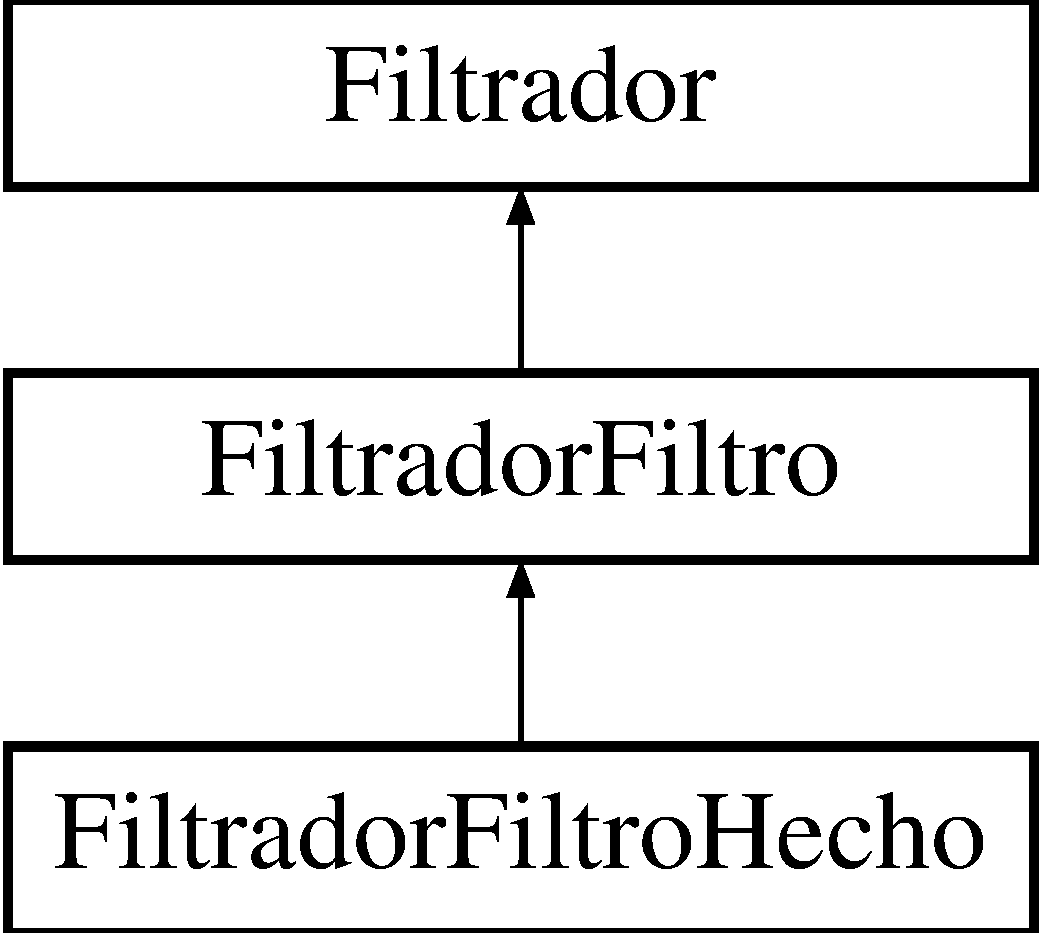
\includegraphics[height=3.000000cm]{classFiltradorFiltroHecho}
\end{center}
\end{figure}
\subsection*{\-Métodos públicos}
\begin{DoxyCompactItemize}
\item 
\hyperlink{classFiltradorFiltroHecho_a7b39688beadb39e91f628302074ca44e}{\-Filtrador\-Filtro\-Hecho} (const \-Glib\-::ustring \&hecho, const \-Glib\-::ustring \&valor\-Combo, const std\-::string \&valor\-Entrada)
\item 
\hyperlink{classFiltradorFiltroHecho_a28657def013a181ed7e8c12a1cc04c31}{$\sim$\-Filtrador\-Filtro\-Hecho} ()
\item 
void \hyperlink{classFiltradorFiltroHecho_a87413cf51710bfd0813d0db87c9a1c11}{filtrar} (\hyperlink{classConsulta}{\-Consulta} \&c)
\end{DoxyCompactItemize}


\subsection{\-Descripción detallada}
\-Filtro de tipo hecho. 

\subsection{\-Documentación del constructor y destructor}
\hypertarget{classFiltradorFiltroHecho_a7b39688beadb39e91f628302074ca44e}{\index{\-Filtrador\-Filtro\-Hecho@{\-Filtrador\-Filtro\-Hecho}!\-Filtrador\-Filtro\-Hecho@{\-Filtrador\-Filtro\-Hecho}}
\index{\-Filtrador\-Filtro\-Hecho@{\-Filtrador\-Filtro\-Hecho}!FiltradorFiltroHecho@{\-Filtrador\-Filtro\-Hecho}}
\subsubsection[{\-Filtrador\-Filtro\-Hecho}]{\setlength{\rightskip}{0pt plus 5cm}{\bf \-Filtrador\-Filtro\-Hecho\-::\-Filtrador\-Filtro\-Hecho} (
\begin{DoxyParamCaption}
\item[{const \-Glib\-::ustring \&}]{hecho, }
\item[{const \-Glib\-::ustring \&}]{valor\-Combo, }
\item[{const std\-::string \&}]{valor\-Entrada}
\end{DoxyParamCaption}
)}}\label{classFiltradorFiltroHecho_a7b39688beadb39e91f628302074ca44e}
\-Constructor. \hypertarget{classFiltradorFiltroHecho_a28657def013a181ed7e8c12a1cc04c31}{\index{\-Filtrador\-Filtro\-Hecho@{\-Filtrador\-Filtro\-Hecho}!$\sim$\-Filtrador\-Filtro\-Hecho@{$\sim$\-Filtrador\-Filtro\-Hecho}}
\index{$\sim$\-Filtrador\-Filtro\-Hecho@{$\sim$\-Filtrador\-Filtro\-Hecho}!FiltradorFiltroHecho@{\-Filtrador\-Filtro\-Hecho}}
\subsubsection[{$\sim$\-Filtrador\-Filtro\-Hecho}]{\setlength{\rightskip}{0pt plus 5cm}{\bf \-Filtrador\-Filtro\-Hecho\-::$\sim$\-Filtrador\-Filtro\-Hecho} (
\begin{DoxyParamCaption}
{}
\end{DoxyParamCaption}
)}}\label{classFiltradorFiltroHecho_a28657def013a181ed7e8c12a1cc04c31}
\-Destructor. 

\subsection{\-Documentación de las funciones miembro}
\hypertarget{classFiltradorFiltroHecho_a87413cf51710bfd0813d0db87c9a1c11}{\index{\-Filtrador\-Filtro\-Hecho@{\-Filtrador\-Filtro\-Hecho}!filtrar@{filtrar}}
\index{filtrar@{filtrar}!FiltradorFiltroHecho@{\-Filtrador\-Filtro\-Hecho}}
\subsubsection[{filtrar}]{\setlength{\rightskip}{0pt plus 5cm}void {\bf \-Filtrador\-Filtro\-Hecho\-::filtrar} (
\begin{DoxyParamCaption}
\item[{{\bf \-Consulta} \&}]{c}
\end{DoxyParamCaption}
)\hspace{0.3cm}{\ttfamily  \mbox{[}virtual\mbox{]}}}}\label{classFiltradorFiltroHecho_a87413cf51710bfd0813d0db87c9a1c11}
\-Agrega su aporte a la consulta. 
\begin{DoxyParams}{\-Parámetros}
{\em c} & consulta \\
\hline
\end{DoxyParams}


\-Implementa \hyperlink{classFiltrador_a5c0739dd669ef0de7f2624c77beb14f0}{\-Filtrador}.



\-La documentación para esta clase fue generada a partir de los siguientes ficheros\-:\begin{DoxyCompactItemize}
\item 
cliente/\-Vista/\-Filtrador\-Filtro\-Hecho.\-h\item 
cliente/\-Vista/\-Filtrador\-Filtro\-Hecho.\-cpp\end{DoxyCompactItemize}

\hypertarget{classFiltradorHelper}{\section{\-Referencia de la \-Clase \-Filtrador\-Helper}
\label{classFiltradorHelper}\index{\-Filtrador\-Helper@{\-Filtrador\-Helper}}
}


{\ttfamily \#include $<$\-Filtrador\-Helper.\-h$>$}

\subsection*{\-Métodos públicos}
\begin{DoxyCompactItemize}
\item 
\hypertarget{classFiltradorHelper_a44da10526a5a9813f6fc689205f33d6e}{void {\bfseries popular\-Combo\-Fecha} (\-Gtk\-::\-Combo\-Box\-Text $\ast$combo) const }\label{classFiltradorHelper_a44da10526a5a9813f6fc689205f33d6e}

\item 
\hypertarget{classFiltradorHelper_a0f4fbd4496e7f7d25d3e16d19f5c016f}{void {\bfseries popular\-Combo\-Hecho\-Input} (\-Gtk\-::\-Combo\-Box\-Text $\ast$combo) const }\label{classFiltradorHelper_a0f4fbd4496e7f7d25d3e16d19f5c016f}

\item 
\hypertarget{classFiltradorHelper_a1f8de0e2977088a0a8d6063fa6b7500e}{void {\bfseries popular\-Combo\-Agregaciones} (\-Gtk\-::\-Combo\-Box\-Text $\ast$combo) const }\label{classFiltradorHelper_a1f8de0e2977088a0a8d6063fa6b7500e}

\item 
\hypertarget{classFiltradorHelper_a7843f8f831fd645fc141f1405e310de7}{int {\bfseries pertenece\-Al\-Combo\-Fecha} (const \-Glib\-::ustring \&valor) const }\label{classFiltradorHelper_a7843f8f831fd645fc141f1405e310de7}

\item 
\hypertarget{classFiltradorHelper_ac50d803953d4e5a0c2ba309453f4940c}{int {\bfseries pertenece\-Al\-Combo\-Hecho\-Input} (const \-Glib\-::ustring \&valor) const }\label{classFiltradorHelper_ac50d803953d4e5a0c2ba309453f4940c}

\item 
\hypertarget{classFiltradorHelper_ad155e8c6b67f780f790a144128d5a467}{int {\bfseries pertenece\-Al\-Agregaciones\-Posibles} (const \-Glib\-::ustring \&valor) const }\label{classFiltradorHelper_ad155e8c6b67f780f790a144128d5a467}

\item 
\hypertarget{classFiltradorHelper_a4fd7f1c5e3b36dd1055a0401a34101f7}{\-Fecha {\bfseries validar\-Fecha} (int i\-\_\-combo, const \-Glib\-::ustring \&valor) const }\label{classFiltradorHelper_a4fd7f1c5e3b36dd1055a0401a34101f7}

\item 
\hypertarget{classFiltradorHelper_aa6a851524b5b9689fe818d641c096e22}{\-Glib\-::ustring {\bfseries validar\-Hecho} (int i\-\_\-combo, const \-Glib\-::ustring \&valor) const }\label{classFiltradorHelper_aa6a851524b5b9689fe818d641c096e22}

\item 
\hypertarget{classFiltradorHelper_a33ea568c98f6c0e715eaf3cc1edc2ed1}{\-Agregacion {\bfseries get\-Agregacion} (int i\-\_\-combo) const }\label{classFiltradorHelper_a33ea568c98f6c0e715eaf3cc1edc2ed1}

\item 
\hypertarget{classFiltradorHelper_a1cb088d7862c15c61ecc7c2471537a82}{\-Glib\-::ustring {\bfseries get\-Valor\-Combo\-Fecha\-Para\-Navegacion} () const }\label{classFiltradorHelper_a1cb088d7862c15c61ecc7c2471537a82}

\end{DoxyCompactItemize}
\subsection*{\-Métodos públicos estáticos}
\begin{DoxyCompactItemize}
\item 
\hypertarget{classFiltradorHelper_adf32e66f6fdc34c0fbfef9c01c55353d}{static const \hyperlink{classFiltradorHelper}{\-Filtrador\-Helper} \& {\bfseries get\-Instancia} ()}\label{classFiltradorHelper_adf32e66f6fdc34c0fbfef9c01c55353d}

\end{DoxyCompactItemize}


\subsection{\-Descripción detallada}
\-Singleton. \-Clase que sólo sirve por su capacidad de\-: -\/popular los combobox que no sean por consulta y validar selecciones de filtradores estáticos -\/validar entradas -\/funcionalidades menores 

\-La documentación para esta clase fue generada a partir de los siguientes ficheros\-:\begin{DoxyCompactItemize}
\item 
cliente/\-Modelo/\-Filtrador\-Helper.\-h\item 
cliente/\-Modelo/\-Filtrador\-Helper.\-cpp\end{DoxyCompactItemize}

\hypertarget{classFiltradorInput}{\section{\-Referencia de la \-Clase \-Filtrador\-Input}
\label{classFiltradorInput}\index{\-Filtrador\-Input@{\-Filtrador\-Input}}
}


{\ttfamily \#include $<$\-Filtrador\-Input.\-h$>$}

\-Diagrama de herencias de \-Filtrador\-Input\begin{figure}[H]
\begin{center}
\leavevmode
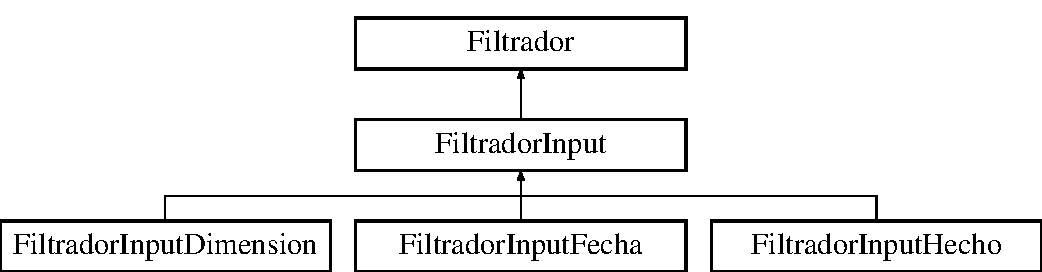
\includegraphics[height=3.000000cm]{classFiltradorInput}
\end{center}
\end{figure}
\subsection*{\-Métodos públicos}
\begin{DoxyCompactItemize}
\item 
\hyperlink{classFiltradorInput_a36209dac5c768231d5ad630ea3676ad8}{\-Filtrador\-Input} (const \-Glib\-::ustring \&input)
\item 
virtual \hyperlink{classFiltradorInput_aaaaf737370b6cf9fbf7d6d00f524fb33}{$\sim$\-Filtrador\-Input} ()
\item 
\hypertarget{classFiltradorInput_abea40f0c14afff6589aea9c61afb1a24}{virtual void {\bfseries recibir\-Navegacion\-Seleccionada} (const \-Glib\-::ustring \&input, const \-Glib\-::ustring \&valor)=0}\label{classFiltradorInput_abea40f0c14afff6589aea9c61afb1a24}

\item 
\hypertarget{classFiltradorInput_a16bb2d588c5397acf42b2b64f1d8f2b9}{void {\bfseries set\-Tab\-Padre} (\hyperlink{classTab}{\-Tab} $\ast$padre)}\label{classFiltradorInput_a16bb2d588c5397acf42b2b64f1d8f2b9}

\item 
\hypertarget{classFiltradorInput_a290ba2ec379f053c78a5e9c56ddae6ab}{sigc\-::signal$<$ void $>$ {\bfseries signal\-\_\-navegabilidad} ()}\label{classFiltradorInput_a290ba2ec379f053c78a5e9c56ddae6ab}

\item 
\hypertarget{classFiltradorInput_a94bf43964d954a7fb30aa6101e930eff}{sigc\-::signal$<$ void, bool $>$ {\bfseries signal\-\_\-input\-\_\-disponible} ()}\label{classFiltradorInput_a94bf43964d954a7fb30aa6101e930eff}

\end{DoxyCompactItemize}
\subsection*{\-Atributos protegidos}
\begin{DoxyCompactItemize}
\item 
\hypertarget{classFiltradorInput_a4f0f46abfa1c45f653f39192760f5941}{\-Gtk\-::\-Combo\-Box\-Text {\bfseries valores}}\label{classFiltradorInput_a4f0f46abfa1c45f653f39192760f5941}

\item 
\hypertarget{classFiltradorInput_a9724b0fac6158d2f7b837b7f89f5ccdc}{bool {\bfseries valido}}\label{classFiltradorInput_a9724b0fac6158d2f7b837b7f89f5ccdc}

\item 
\hypertarget{classFiltradorInput_aa3ff49b92eca82bcbc5ceeb0d62cec28}{\hyperlink{classTab}{\-Tab} $\ast$ {\bfseries tab\-Padre}}\label{classFiltradorInput_aa3ff49b92eca82bcbc5ceeb0d62cec28}

\item 
\hypertarget{classFiltradorInput_a02476cd0aaba6694408262b53de60695}{sigc\-::signal$<$ void $>$ {\bfseries signal\-\_\-navegabilidad\-\_\-seleccionada}}\label{classFiltradorInput_a02476cd0aaba6694408262b53de60695}

\item 
\hypertarget{classFiltradorInput_a224415e45d4b0cbf4c33388760a7646f}{sigc\-::signal$<$ void, bool $>$ {\bfseries \-\_\-signal\-\_\-input\-\_\-disponible}}\label{classFiltradorInput_a224415e45d4b0cbf4c33388760a7646f}

\end{DoxyCompactItemize}


\subsection{\-Descripción detallada}
\hyperlink{classFiltrador}{\-Filtrador} concretado en un input. \-Puede interpretar navegabilidad seleccionada. \-Como todavía varía según la entrada sea un hecho, dimensión o fecha, sigue siendo una clase abstracta. 

\subsection{\-Documentación del constructor y destructor}
\hypertarget{classFiltradorInput_a36209dac5c768231d5ad630ea3676ad8}{\index{\-Filtrador\-Input@{\-Filtrador\-Input}!\-Filtrador\-Input@{\-Filtrador\-Input}}
\index{\-Filtrador\-Input@{\-Filtrador\-Input}!FiltradorInput@{\-Filtrador\-Input}}
\subsubsection[{\-Filtrador\-Input}]{\setlength{\rightskip}{0pt plus 5cm}{\bf \-Filtrador\-Input\-::\-Filtrador\-Input} (
\begin{DoxyParamCaption}
\item[{const \-Glib\-::ustring \&}]{input}
\end{DoxyParamCaption}
)}}\label{classFiltradorInput_a36209dac5c768231d5ad630ea3676ad8}
\-Constructor. 
\begin{DoxyParams}{\-Parámetros}
{\em input} & nombre del campo \\
\hline
\end{DoxyParams}
\hypertarget{classFiltradorInput_aaaaf737370b6cf9fbf7d6d00f524fb33}{\index{\-Filtrador\-Input@{\-Filtrador\-Input}!$\sim$\-Filtrador\-Input@{$\sim$\-Filtrador\-Input}}
\index{$\sim$\-Filtrador\-Input@{$\sim$\-Filtrador\-Input}!FiltradorInput@{\-Filtrador\-Input}}
\subsubsection[{$\sim$\-Filtrador\-Input}]{\setlength{\rightskip}{0pt plus 5cm}{\bf \-Filtrador\-Input\-::$\sim$\-Filtrador\-Input} (
\begin{DoxyParamCaption}
{}
\end{DoxyParamCaption}
)\hspace{0.3cm}{\ttfamily  \mbox{[}virtual\mbox{]}}}}\label{classFiltradorInput_aaaaf737370b6cf9fbf7d6d00f524fb33}
\-Destructor. 

\-La documentación para esta clase fue generada a partir de los siguientes ficheros\-:\begin{DoxyCompactItemize}
\item 
cliente/\-Vista/\-Filtrador\-Input.\-h\item 
cliente/\-Vista/\-Filtrador\-Input.\-cpp\end{DoxyCompactItemize}

\hypertarget{classFiltradorInputDimension}{\section{\-Referencia de la \-Clase \-Filtrador\-Input\-Dimension}
\label{classFiltradorInputDimension}\index{\-Filtrador\-Input\-Dimension@{\-Filtrador\-Input\-Dimension}}
}


{\ttfamily \#include $<$\-Filtrador\-Input\-Dimension.\-h$>$}

\-Diagrama de herencias de \-Filtrador\-Input\-Dimension\begin{figure}[H]
\begin{center}
\leavevmode
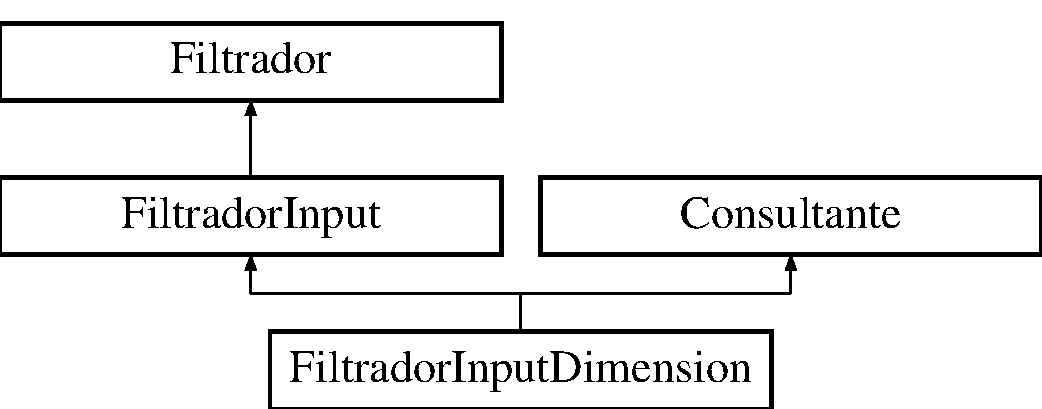
\includegraphics[height=3.000000cm]{classFiltradorInputDimension}
\end{center}
\end{figure}
\subsection*{\-Métodos públicos}
\begin{DoxyCompactItemize}
\item 
\hyperlink{classFiltradorInputDimension_a4ca75aee43080e33ccb421297d4ff10e}{\-Filtrador\-Input\-Dimension} (const \-Glib\-::ustring \&input)
\item 
\hyperlink{classFiltradorInputDimension_ad2dbe4b65f21da8fd23264122d70f250}{$\sim$\-Filtrador\-Input\-Dimension} ()
\item 
void \hyperlink{classFiltradorInputDimension_a18da290896d3d045a31127f613d12a1c}{filtrar} (\hyperlink{classConsulta}{\-Consulta} \&c)
\item 
\hypertarget{classFiltradorInputDimension_aca8bed224cce07cfe437c32b4f2bb584}{void {\bfseries recibir\-Navegacion\-Seleccionada} (const \-Glib\-::ustring \&input, const \-Glib\-::ustring \&valor)}\label{classFiltradorInputDimension_aca8bed224cce07cfe437c32b4f2bb584}

\end{DoxyCompactItemize}


\subsection{\-Descripción detallada}
\-Input de comportamiento \char`\"{}básico\char`\"{}, es decir, no es hecho ni fecha. 

\subsection{\-Documentación del constructor y destructor}
\hypertarget{classFiltradorInputDimension_a4ca75aee43080e33ccb421297d4ff10e}{\index{\-Filtrador\-Input\-Dimension@{\-Filtrador\-Input\-Dimension}!\-Filtrador\-Input\-Dimension@{\-Filtrador\-Input\-Dimension}}
\index{\-Filtrador\-Input\-Dimension@{\-Filtrador\-Input\-Dimension}!FiltradorInputDimension@{\-Filtrador\-Input\-Dimension}}
\subsubsection[{\-Filtrador\-Input\-Dimension}]{\setlength{\rightskip}{0pt plus 5cm}{\bf \-Filtrador\-Input\-Dimension\-::\-Filtrador\-Input\-Dimension} (
\begin{DoxyParamCaption}
\item[{const \-Glib\-::ustring \&}]{input}
\end{DoxyParamCaption}
)}}\label{classFiltradorInputDimension_a4ca75aee43080e33ccb421297d4ff10e}
\-Constructor. 
\begin{DoxyParams}{\-Parámetros}
{\em input} & nombre de la dimensión elegida \\
\hline
\end{DoxyParams}
\hypertarget{classFiltradorInputDimension_ad2dbe4b65f21da8fd23264122d70f250}{\index{\-Filtrador\-Input\-Dimension@{\-Filtrador\-Input\-Dimension}!$\sim$\-Filtrador\-Input\-Dimension@{$\sim$\-Filtrador\-Input\-Dimension}}
\index{$\sim$\-Filtrador\-Input\-Dimension@{$\sim$\-Filtrador\-Input\-Dimension}!FiltradorInputDimension@{\-Filtrador\-Input\-Dimension}}
\subsubsection[{$\sim$\-Filtrador\-Input\-Dimension}]{\setlength{\rightskip}{0pt plus 5cm}{\bf \-Filtrador\-Input\-Dimension\-::$\sim$\-Filtrador\-Input\-Dimension} (
\begin{DoxyParamCaption}
{}
\end{DoxyParamCaption}
)}}\label{classFiltradorInputDimension_ad2dbe4b65f21da8fd23264122d70f250}
\-Destructor. 

\subsection{\-Documentación de las funciones miembro}
\hypertarget{classFiltradorInputDimension_a18da290896d3d045a31127f613d12a1c}{\index{\-Filtrador\-Input\-Dimension@{\-Filtrador\-Input\-Dimension}!filtrar@{filtrar}}
\index{filtrar@{filtrar}!FiltradorInputDimension@{\-Filtrador\-Input\-Dimension}}
\subsubsection[{filtrar}]{\setlength{\rightskip}{0pt plus 5cm}void {\bf \-Filtrador\-Input\-Dimension\-::filtrar} (
\begin{DoxyParamCaption}
\item[{{\bf \-Consulta} \&}]{c}
\end{DoxyParamCaption}
)\hspace{0.3cm}{\ttfamily  \mbox{[}virtual\mbox{]}}}}\label{classFiltradorInputDimension_a18da290896d3d045a31127f613d12a1c}
\-Agrega el input a la consulta. 
\begin{DoxyParams}{\-Parámetros}
{\em c} & consulta \\
\hline
\end{DoxyParams}


\-Implementa \hyperlink{classFiltrador_a5c0739dd669ef0de7f2624c77beb14f0}{\-Filtrador}.



\-La documentación para esta clase fue generada a partir de los siguientes ficheros\-:\begin{DoxyCompactItemize}
\item 
cliente/\-Vista/\-Filtrador\-Input\-Dimension.\-h\item 
cliente/\-Vista/\-Filtrador\-Input\-Dimension.\-cpp\end{DoxyCompactItemize}

\hypertarget{classFiltradorInputFecha}{\section{\-Referencia de la \-Clase \-Filtrador\-Input\-Fecha}
\label{classFiltradorInputFecha}\index{\-Filtrador\-Input\-Fecha@{\-Filtrador\-Input\-Fecha}}
}


{\ttfamily \#include $<$\-Filtrador\-Input\-Fecha.\-h$>$}

\-Diagrama de herencias de \-Filtrador\-Input\-Fecha\begin{figure}[H]
\begin{center}
\leavevmode
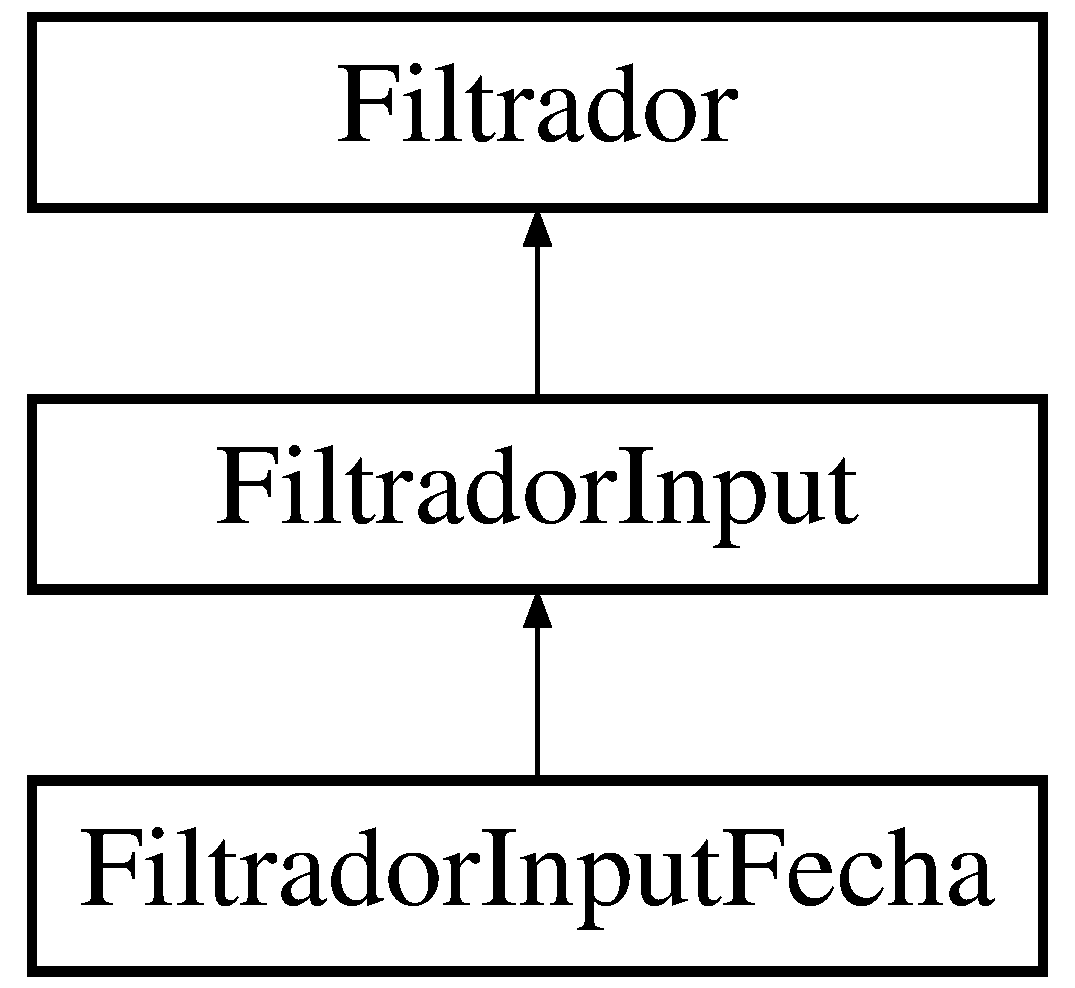
\includegraphics[height=3.000000cm]{classFiltradorInputFecha}
\end{center}
\end{figure}
\subsection*{\-Métodos públicos}
\begin{DoxyCompactItemize}
\item 
\hyperlink{classFiltradorInputFecha_af3194e39d85744b3755361ed508daba6}{\-Filtrador\-Input\-Fecha} (const \-Glib\-::ustring \&input)
\item 
\hyperlink{classFiltradorInputFecha_a23948a5fa09756f32d3f2a66a465631d}{$\sim$\-Filtrador\-Input\-Fecha} ()
\item 
\hypertarget{classFiltradorInputFecha_afc1e623ea9571ca1ddbcdedda625ce60}{void {\bfseries recibir\-Navegacion\-Seleccionada} (const \-Glib\-::ustring \&input, const \-Glib\-::ustring \&valor)}\label{classFiltradorInputFecha_afc1e623ea9571ca1ddbcdedda625ce60}

\item 
void \hyperlink{classFiltradorInputFecha_a4ca7340057566a1247bc082ba94dad25}{filtrar} (\hyperlink{classConsulta}{\-Consulta} \&c)
\end{DoxyCompactItemize}


\subsection{\-Descripción detallada}
\-Input de tipo fecha. 

\subsection{\-Documentación del constructor y destructor}
\hypertarget{classFiltradorInputFecha_af3194e39d85744b3755361ed508daba6}{\index{\-Filtrador\-Input\-Fecha@{\-Filtrador\-Input\-Fecha}!\-Filtrador\-Input\-Fecha@{\-Filtrador\-Input\-Fecha}}
\index{\-Filtrador\-Input\-Fecha@{\-Filtrador\-Input\-Fecha}!FiltradorInputFecha@{\-Filtrador\-Input\-Fecha}}
\subsubsection[{\-Filtrador\-Input\-Fecha}]{\setlength{\rightskip}{0pt plus 5cm}{\bf \-Filtrador\-Input\-Fecha\-::\-Filtrador\-Input\-Fecha} (
\begin{DoxyParamCaption}
\item[{const \-Glib\-::ustring \&}]{input}
\end{DoxyParamCaption}
)}}\label{classFiltradorInputFecha_af3194e39d85744b3755361ed508daba6}
\-Constructor. 
\begin{DoxyParams}{\-Parámetros}
{\em input} & nombre del campo fecha \\
\hline
\end{DoxyParams}
\hypertarget{classFiltradorInputFecha_a23948a5fa09756f32d3f2a66a465631d}{\index{\-Filtrador\-Input\-Fecha@{\-Filtrador\-Input\-Fecha}!$\sim$\-Filtrador\-Input\-Fecha@{$\sim$\-Filtrador\-Input\-Fecha}}
\index{$\sim$\-Filtrador\-Input\-Fecha@{$\sim$\-Filtrador\-Input\-Fecha}!FiltradorInputFecha@{\-Filtrador\-Input\-Fecha}}
\subsubsection[{$\sim$\-Filtrador\-Input\-Fecha}]{\setlength{\rightskip}{0pt plus 5cm}{\bf \-Filtrador\-Input\-Fecha\-::$\sim$\-Filtrador\-Input\-Fecha} (
\begin{DoxyParamCaption}
{}
\end{DoxyParamCaption}
)}}\label{classFiltradorInputFecha_a23948a5fa09756f32d3f2a66a465631d}
\-Destructor. 

\subsection{\-Documentación de las funciones miembro}
\hypertarget{classFiltradorInputFecha_a4ca7340057566a1247bc082ba94dad25}{\index{\-Filtrador\-Input\-Fecha@{\-Filtrador\-Input\-Fecha}!filtrar@{filtrar}}
\index{filtrar@{filtrar}!FiltradorInputFecha@{\-Filtrador\-Input\-Fecha}}
\subsubsection[{filtrar}]{\setlength{\rightskip}{0pt plus 5cm}void {\bf \-Filtrador\-Input\-Fecha\-::filtrar} (
\begin{DoxyParamCaption}
\item[{{\bf \-Consulta} \&}]{c}
\end{DoxyParamCaption}
)\hspace{0.3cm}{\ttfamily  \mbox{[}virtual\mbox{]}}}}\label{classFiltradorInputFecha_a4ca7340057566a1247bc082ba94dad25}
\-Agrega el input a la consulta. 
\begin{DoxyParams}{\-Parámetros}
{\em c} & consulta \\
\hline
\end{DoxyParams}


\-Implementa \hyperlink{classFiltrador_a5c0739dd669ef0de7f2624c77beb14f0}{\-Filtrador}.



\-La documentación para esta clase fue generada a partir de los siguientes ficheros\-:\begin{DoxyCompactItemize}
\item 
cliente/\-Vista/\-Filtrador\-Input\-Fecha.\-h\item 
cliente/\-Vista/\-Filtrador\-Input\-Fecha.\-cpp\end{DoxyCompactItemize}

\hypertarget{classFiltradorInputHecho}{\section{\-Referencia de la \-Clase \-Filtrador\-Input\-Hecho}
\label{classFiltradorInputHecho}\index{\-Filtrador\-Input\-Hecho@{\-Filtrador\-Input\-Hecho}}
}


{\ttfamily \#include $<$\-Filtrador\-Input\-Hecho.\-h$>$}

\-Diagrama de herencias de \-Filtrador\-Input\-Hecho\begin{figure}[H]
\begin{center}
\leavevmode
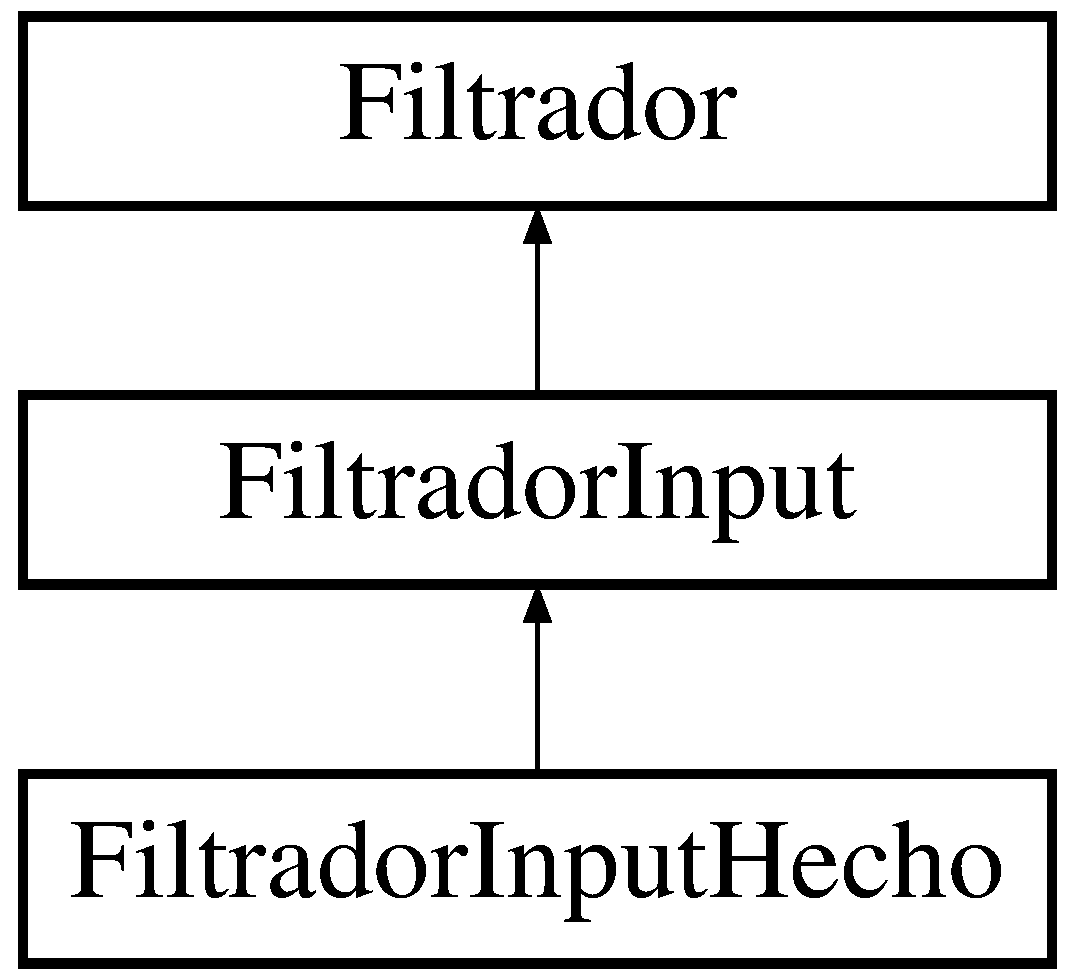
\includegraphics[height=3.000000cm]{classFiltradorInputHecho}
\end{center}
\end{figure}
\subsection*{\-Métodos públicos}
\begin{DoxyCompactItemize}
\item 
\hyperlink{classFiltradorInputHecho_a24dd6f3beba32f9b2e6a988174513cd3}{\-Filtrador\-Input\-Hecho} (const \-Glib\-::ustring \&input)
\item 
\hyperlink{classFiltradorInputHecho_a3abb02b0b016bd2d58012c41ae21bfad}{$\sim$\-Filtrador\-Input\-Hecho} ()
\item 
\hypertarget{classFiltradorInputHecho_a0f17d36d1e33e28e348d317168fa8301}{void {\bfseries recibir\-Navegacion\-Seleccionada} (const \-Glib\-::ustring \&input, const \-Glib\-::ustring \&valor)}\label{classFiltradorInputHecho_a0f17d36d1e33e28e348d317168fa8301}

\item 
void \hyperlink{classFiltradorInputHecho_adaaa9cddc3f560961b108acfc8a002f9}{filtrar} (\hyperlink{classConsulta}{\-Consulta} \&c)
\end{DoxyCompactItemize}


\subsection{\-Descripción detallada}
\-Input de tipo hecho. 

\subsection{\-Documentación del constructor y destructor}
\hypertarget{classFiltradorInputHecho_a24dd6f3beba32f9b2e6a988174513cd3}{\index{\-Filtrador\-Input\-Hecho@{\-Filtrador\-Input\-Hecho}!\-Filtrador\-Input\-Hecho@{\-Filtrador\-Input\-Hecho}}
\index{\-Filtrador\-Input\-Hecho@{\-Filtrador\-Input\-Hecho}!FiltradorInputHecho@{\-Filtrador\-Input\-Hecho}}
\subsubsection[{\-Filtrador\-Input\-Hecho}]{\setlength{\rightskip}{0pt plus 5cm}{\bf \-Filtrador\-Input\-Hecho\-::\-Filtrador\-Input\-Hecho} (
\begin{DoxyParamCaption}
\item[{const \-Glib\-::ustring \&}]{input}
\end{DoxyParamCaption}
)}}\label{classFiltradorInputHecho_a24dd6f3beba32f9b2e6a988174513cd3}
\-Constructor. 
\begin{DoxyParams}{\-Parámetros}
{\em input} & nombre del hecho \\
\hline
\end{DoxyParams}
\hypertarget{classFiltradorInputHecho_a3abb02b0b016bd2d58012c41ae21bfad}{\index{\-Filtrador\-Input\-Hecho@{\-Filtrador\-Input\-Hecho}!$\sim$\-Filtrador\-Input\-Hecho@{$\sim$\-Filtrador\-Input\-Hecho}}
\index{$\sim$\-Filtrador\-Input\-Hecho@{$\sim$\-Filtrador\-Input\-Hecho}!FiltradorInputHecho@{\-Filtrador\-Input\-Hecho}}
\subsubsection[{$\sim$\-Filtrador\-Input\-Hecho}]{\setlength{\rightskip}{0pt plus 5cm}{\bf \-Filtrador\-Input\-Hecho\-::$\sim$\-Filtrador\-Input\-Hecho} (
\begin{DoxyParamCaption}
{}
\end{DoxyParamCaption}
)}}\label{classFiltradorInputHecho_a3abb02b0b016bd2d58012c41ae21bfad}
\-Destructor. 

\subsection{\-Documentación de las funciones miembro}
\hypertarget{classFiltradorInputHecho_adaaa9cddc3f560961b108acfc8a002f9}{\index{\-Filtrador\-Input\-Hecho@{\-Filtrador\-Input\-Hecho}!filtrar@{filtrar}}
\index{filtrar@{filtrar}!FiltradorInputHecho@{\-Filtrador\-Input\-Hecho}}
\subsubsection[{filtrar}]{\setlength{\rightskip}{0pt plus 5cm}void {\bf \-Filtrador\-Input\-Hecho\-::filtrar} (
\begin{DoxyParamCaption}
\item[{{\bf \-Consulta} \&}]{c}
\end{DoxyParamCaption}
)\hspace{0.3cm}{\ttfamily  \mbox{[}virtual\mbox{]}}}}\label{classFiltradorInputHecho_adaaa9cddc3f560961b108acfc8a002f9}
\-Agrega el input a la consulta. 
\begin{DoxyParams}{\-Parámetros}
{\em c} & consulta \\
\hline
\end{DoxyParams}


\-Implementa \hyperlink{classFiltrador_a5c0739dd669ef0de7f2624c77beb14f0}{\-Filtrador}.



\-La documentación para esta clase fue generada a partir de los siguientes ficheros\-:\begin{DoxyCompactItemize}
\item 
cliente/\-Vista/\-Filtrador\-Input\-Hecho.\-h\item 
cliente/\-Vista/\-Filtrador\-Input\-Hecho.\-cpp\end{DoxyCompactItemize}

\hypertarget{classFiltradorPivoteX}{\section{\-Referencia de la \-Clase \-Filtrador\-Pivote\-X}
\label{classFiltradorPivoteX}\index{\-Filtrador\-Pivote\-X@{\-Filtrador\-Pivote\-X}}
}


{\ttfamily \#include $<$\-Filtrador\-Pivote\-X.\-h$>$}

\-Diagrama de herencias de \-Filtrador\-Pivote\-X\begin{figure}[H]
\begin{center}
\leavevmode
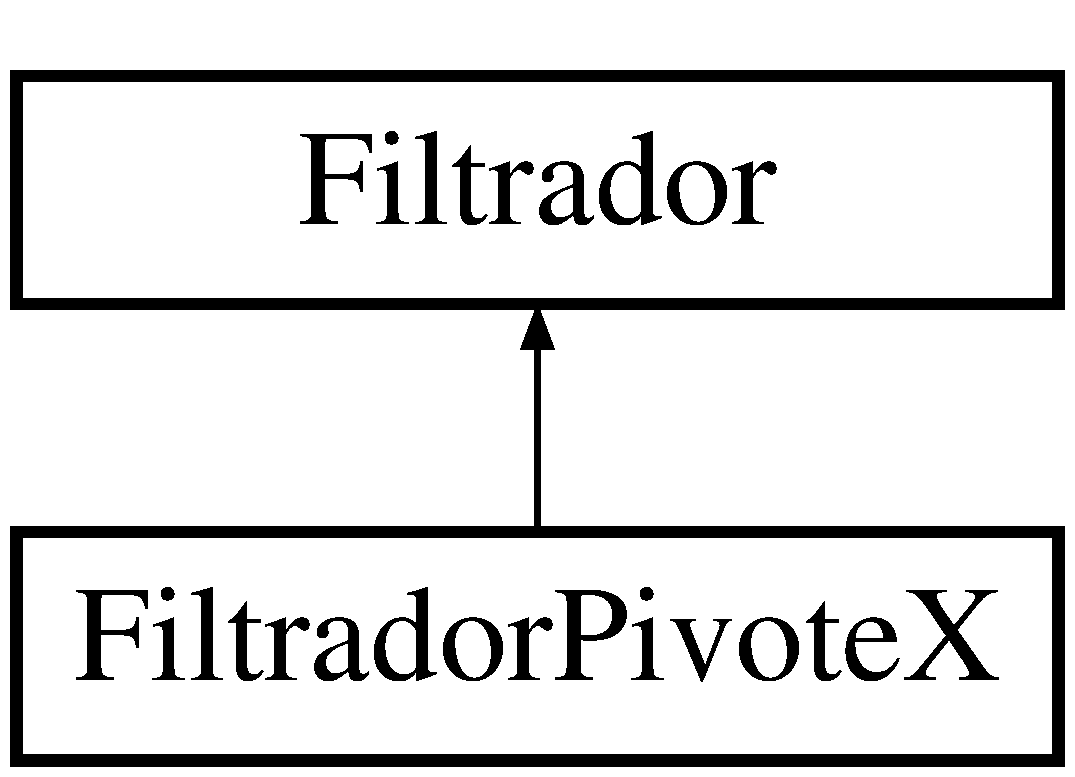
\includegraphics[height=2.000000cm]{classFiltradorPivoteX}
\end{center}
\end{figure}
\subsection*{\-Métodos públicos}
\begin{DoxyCompactItemize}
\item 
\hyperlink{classFiltradorPivoteX_af0105c06871741244f626c59fd181a77}{\-Filtrador\-Pivote\-X} (const \-Glib\-::ustring \&valor)
\item 
\hyperlink{classFiltradorPivoteX_a3af2e0db4c29a405f4f8c860b01579c0}{$\sim$\-Filtrador\-Pivote\-X} ()
\item 
void \hyperlink{classFiltradorPivoteX_aac8f278c7e313efdbaca2aea28730c90}{filtrar} (\hyperlink{classConsulta}{\-Consulta} \&c)
\end{DoxyCompactItemize}


\subsection{\-Descripción detallada}
\hyperlink{classFiltrador}{\-Filtrador} concretado en un elemento de \-X de la tabla pivote. 

\subsection{\-Documentación del constructor y destructor}
\hypertarget{classFiltradorPivoteX_af0105c06871741244f626c59fd181a77}{\index{\-Filtrador\-Pivote\-X@{\-Filtrador\-Pivote\-X}!\-Filtrador\-Pivote\-X@{\-Filtrador\-Pivote\-X}}
\index{\-Filtrador\-Pivote\-X@{\-Filtrador\-Pivote\-X}!FiltradorPivoteX@{\-Filtrador\-Pivote\-X}}
\subsubsection[{\-Filtrador\-Pivote\-X}]{\setlength{\rightskip}{0pt plus 5cm}{\bf \-Filtrador\-Pivote\-X\-::\-Filtrador\-Pivote\-X} (
\begin{DoxyParamCaption}
\item[{const \-Glib\-::ustring \&}]{valor}
\end{DoxyParamCaption}
)}}\label{classFiltradorPivoteX_af0105c06871741244f626c59fd181a77}
\-Constructor. 
\begin{DoxyParams}{\-Parámetros}
{\em valor} & nombre del campo \\
\hline
\end{DoxyParams}
\hypertarget{classFiltradorPivoteX_a3af2e0db4c29a405f4f8c860b01579c0}{\index{\-Filtrador\-Pivote\-X@{\-Filtrador\-Pivote\-X}!$\sim$\-Filtrador\-Pivote\-X@{$\sim$\-Filtrador\-Pivote\-X}}
\index{$\sim$\-Filtrador\-Pivote\-X@{$\sim$\-Filtrador\-Pivote\-X}!FiltradorPivoteX@{\-Filtrador\-Pivote\-X}}
\subsubsection[{$\sim$\-Filtrador\-Pivote\-X}]{\setlength{\rightskip}{0pt plus 5cm}{\bf \-Filtrador\-Pivote\-X\-::$\sim$\-Filtrador\-Pivote\-X} (
\begin{DoxyParamCaption}
{}
\end{DoxyParamCaption}
)}}\label{classFiltradorPivoteX_a3af2e0db4c29a405f4f8c860b01579c0}
\-Destructor. 

\subsection{\-Documentación de las funciones miembro}
\hypertarget{classFiltradorPivoteX_aac8f278c7e313efdbaca2aea28730c90}{\index{\-Filtrador\-Pivote\-X@{\-Filtrador\-Pivote\-X}!filtrar@{filtrar}}
\index{filtrar@{filtrar}!FiltradorPivoteX@{\-Filtrador\-Pivote\-X}}
\subsubsection[{filtrar}]{\setlength{\rightskip}{0pt plus 5cm}void {\bf \-Filtrador\-Pivote\-X\-::filtrar} (
\begin{DoxyParamCaption}
\item[{{\bf \-Consulta} \&}]{c}
\end{DoxyParamCaption}
)\hspace{0.3cm}{\ttfamily  \mbox{[}virtual\mbox{]}}}}\label{classFiltradorPivoteX_aac8f278c7e313efdbaca2aea28730c90}
\-Agrega un elemento al grupo \-X de la consulta de tabla pivote. 
\begin{DoxyParams}{\-Parámetros}
{\em c} & consulta \\
\hline
\end{DoxyParams}


\-Implementa \hyperlink{classFiltrador_a5c0739dd669ef0de7f2624c77beb14f0}{\-Filtrador}.



\-La documentación para esta clase fue generada a partir de los siguientes ficheros\-:\begin{DoxyCompactItemize}
\item 
cliente/\-Vista/\-Filtrador\-Pivote\-X.\-h\item 
cliente/\-Vista/\-Filtrador\-Pivote\-X.\-cpp\end{DoxyCompactItemize}

\hypertarget{classFiltradorPivoteY}{\section{\-Referencia de la \-Clase \-Filtrador\-Pivote\-Y}
\label{classFiltradorPivoteY}\index{\-Filtrador\-Pivote\-Y@{\-Filtrador\-Pivote\-Y}}
}


{\ttfamily \#include $<$\-Filtrador\-Pivote\-Y.\-h$>$}

\-Diagrama de herencias de \-Filtrador\-Pivote\-Y\begin{figure}[H]
\begin{center}
\leavevmode
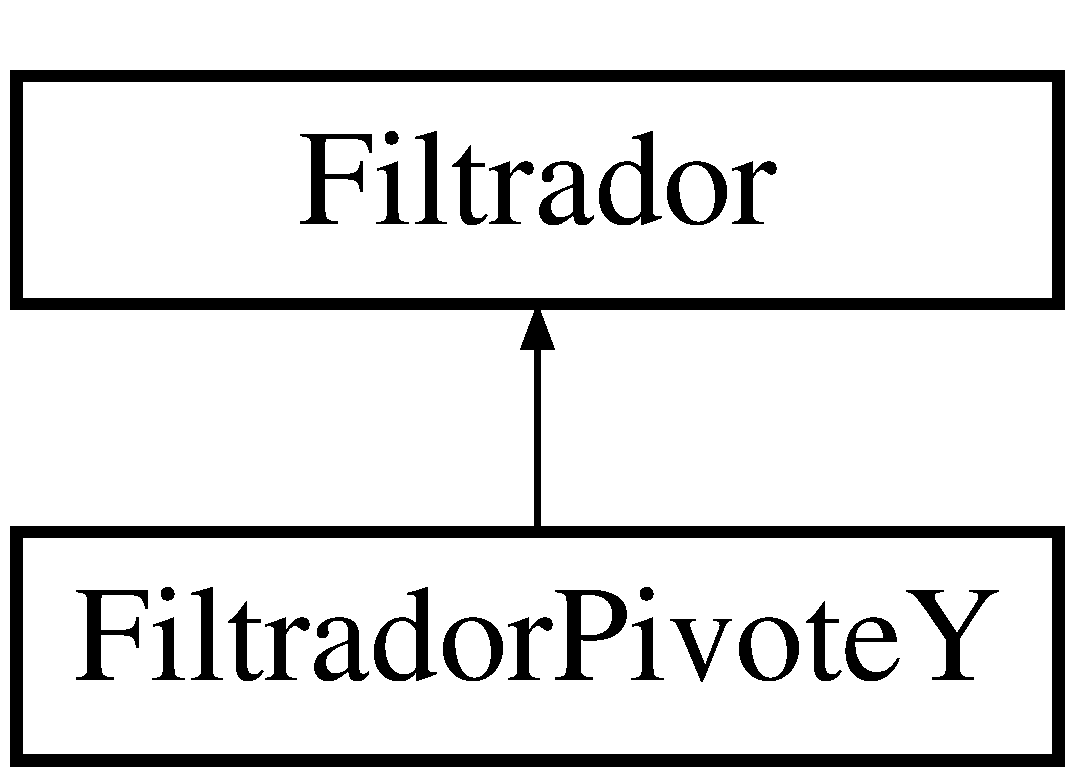
\includegraphics[height=2.000000cm]{classFiltradorPivoteY}
\end{center}
\end{figure}
\subsection*{\-Métodos públicos}
\begin{DoxyCompactItemize}
\item 
\hyperlink{classFiltradorPivoteY_aee366ac39afd3070ee9922899c4b0175}{\-Filtrador\-Pivote\-Y} (const \-Glib\-::ustring \&valor)
\item 
\hyperlink{classFiltradorPivoteY_ac9bedc3d3f4176bd3b8dbe8cf522d596}{$\sim$\-Filtrador\-Pivote\-Y} ()
\item 
void \hyperlink{classFiltradorPivoteY_a66d31de7db52e27c91073a27fd53b835}{filtrar} (\hyperlink{classConsulta}{\-Consulta} \&c)
\end{DoxyCompactItemize}


\subsection{\-Descripción detallada}
\hyperlink{classFiltrador}{\-Filtrador} concretado en un elemento de \-Y de la tabla pivote. 

\subsection{\-Documentación del constructor y destructor}
\hypertarget{classFiltradorPivoteY_aee366ac39afd3070ee9922899c4b0175}{\index{\-Filtrador\-Pivote\-Y@{\-Filtrador\-Pivote\-Y}!\-Filtrador\-Pivote\-Y@{\-Filtrador\-Pivote\-Y}}
\index{\-Filtrador\-Pivote\-Y@{\-Filtrador\-Pivote\-Y}!FiltradorPivoteY@{\-Filtrador\-Pivote\-Y}}
\subsubsection[{\-Filtrador\-Pivote\-Y}]{\setlength{\rightskip}{0pt plus 5cm}{\bf \-Filtrador\-Pivote\-Y\-::\-Filtrador\-Pivote\-Y} (
\begin{DoxyParamCaption}
\item[{const \-Glib\-::ustring \&}]{valor}
\end{DoxyParamCaption}
)}}\label{classFiltradorPivoteY_aee366ac39afd3070ee9922899c4b0175}
\-Constructor. 
\begin{DoxyParams}{\-Parámetros}
{\em valor} & nombre del campo \\
\hline
\end{DoxyParams}
\hypertarget{classFiltradorPivoteY_ac9bedc3d3f4176bd3b8dbe8cf522d596}{\index{\-Filtrador\-Pivote\-Y@{\-Filtrador\-Pivote\-Y}!$\sim$\-Filtrador\-Pivote\-Y@{$\sim$\-Filtrador\-Pivote\-Y}}
\index{$\sim$\-Filtrador\-Pivote\-Y@{$\sim$\-Filtrador\-Pivote\-Y}!FiltradorPivoteY@{\-Filtrador\-Pivote\-Y}}
\subsubsection[{$\sim$\-Filtrador\-Pivote\-Y}]{\setlength{\rightskip}{0pt plus 5cm}{\bf \-Filtrador\-Pivote\-Y\-::$\sim$\-Filtrador\-Pivote\-Y} (
\begin{DoxyParamCaption}
{}
\end{DoxyParamCaption}
)}}\label{classFiltradorPivoteY_ac9bedc3d3f4176bd3b8dbe8cf522d596}
\-Destructor. 

\subsection{\-Documentación de las funciones miembro}
\hypertarget{classFiltradorPivoteY_a66d31de7db52e27c91073a27fd53b835}{\index{\-Filtrador\-Pivote\-Y@{\-Filtrador\-Pivote\-Y}!filtrar@{filtrar}}
\index{filtrar@{filtrar}!FiltradorPivoteY@{\-Filtrador\-Pivote\-Y}}
\subsubsection[{filtrar}]{\setlength{\rightskip}{0pt plus 5cm}void {\bf \-Filtrador\-Pivote\-Y\-::filtrar} (
\begin{DoxyParamCaption}
\item[{{\bf \-Consulta} \&}]{c}
\end{DoxyParamCaption}
)\hspace{0.3cm}{\ttfamily  \mbox{[}virtual\mbox{]}}}}\label{classFiltradorPivoteY_a66d31de7db52e27c91073a27fd53b835}
\-Agrega un elemento al grupo \-Y de la consulta de tabla pivote. 
\begin{DoxyParams}{\-Parámetros}
{\em c} & consulta \\
\hline
\end{DoxyParams}


\-Implementa \hyperlink{classFiltrador_a5c0739dd669ef0de7f2624c77beb14f0}{\-Filtrador}.



\-La documentación para esta clase fue generada a partir de los siguientes ficheros\-:\begin{DoxyCompactItemize}
\item 
cliente/\-Vista/\-Filtrador\-Pivote\-Y.\-h\item 
cliente/\-Vista/\-Filtrador\-Pivote\-Y.\-cpp\end{DoxyCompactItemize}

\hypertarget{classFiltradorResultado}{\section{\-Referencia de la \-Clase \-Filtrador\-Resultado}
\label{classFiltradorResultado}\index{\-Filtrador\-Resultado@{\-Filtrador\-Resultado}}
}


{\ttfamily \#include $<$\-Filtrador\-Resultado.\-h$>$}

\-Diagrama de herencias de \-Filtrador\-Resultado\begin{figure}[H]
\begin{center}
\leavevmode
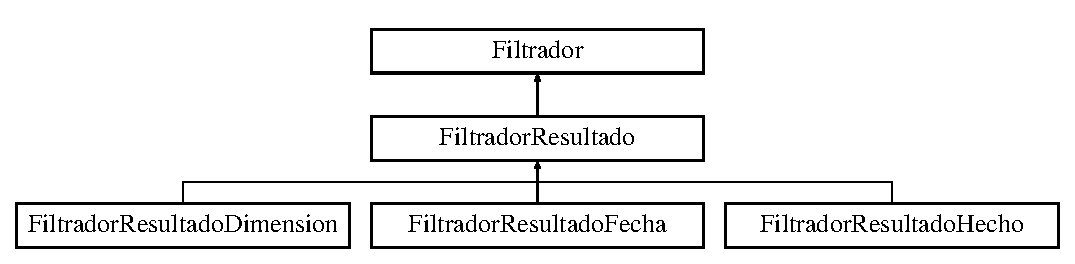
\includegraphics[height=3.000000cm]{classFiltradorResultado}
\end{center}
\end{figure}
\subsection*{\-Métodos públicos}
\begin{DoxyCompactItemize}
\item 
\hyperlink{classFiltradorResultado_a305a76ab5ae0d11fad7977ac5721943f}{\-Filtrador\-Resultado} (const \-Glib\-::ustring \&resultado)
\item 
virtual \hyperlink{classFiltradorResultado_a4a290c0913c74902a0a784cd6d4a4576}{$\sim$\-Filtrador\-Resultado} ()
\end{DoxyCompactItemize}
\subsection*{\-Métodos protegidos}
\begin{DoxyCompactItemize}
\item 
\hypertarget{classFiltradorResultado_a849d09be2b85fc4d0e2ef1ea71b52b0a}{void {\bfseries set\-Resultado} (const \-Glib\-::ustring \&resultado)}\label{classFiltradorResultado_a849d09be2b85fc4d0e2ef1ea71b52b0a}

\item 
\hypertarget{classFiltradorResultado_a4dacaca662d9f373a7bceaec7dd97f9c}{\-Glib\-::ustring {\bfseries get\-Resultado} ()}\label{classFiltradorResultado_a4dacaca662d9f373a7bceaec7dd97f9c}

\end{DoxyCompactItemize}


\subsection{\-Descripción detallada}
\hyperlink{classFiltrador}{\-Filtrador} concretado en un resultado de la consulta. \-Como todavía varía según el resultado sea un hecho, dimensión o fecha, sigue siendo una clase abstracta. 

\subsection{\-Documentación del constructor y destructor}
\hypertarget{classFiltradorResultado_a305a76ab5ae0d11fad7977ac5721943f}{\index{\-Filtrador\-Resultado@{\-Filtrador\-Resultado}!\-Filtrador\-Resultado@{\-Filtrador\-Resultado}}
\index{\-Filtrador\-Resultado@{\-Filtrador\-Resultado}!FiltradorResultado@{\-Filtrador\-Resultado}}
\subsubsection[{\-Filtrador\-Resultado}]{\setlength{\rightskip}{0pt plus 5cm}{\bf \-Filtrador\-Resultado\-::\-Filtrador\-Resultado} (
\begin{DoxyParamCaption}
\item[{const \-Glib\-::ustring \&}]{resultado}
\end{DoxyParamCaption}
)}}\label{classFiltradorResultado_a305a76ab5ae0d11fad7977ac5721943f}
\-Constructor. 
\begin{DoxyParams}{\-Parámetros}
{\em resultado} & nombre del campo \\
\hline
\end{DoxyParams}
\hypertarget{classFiltradorResultado_a4a290c0913c74902a0a784cd6d4a4576}{\index{\-Filtrador\-Resultado@{\-Filtrador\-Resultado}!$\sim$\-Filtrador\-Resultado@{$\sim$\-Filtrador\-Resultado}}
\index{$\sim$\-Filtrador\-Resultado@{$\sim$\-Filtrador\-Resultado}!FiltradorResultado@{\-Filtrador\-Resultado}}
\subsubsection[{$\sim$\-Filtrador\-Resultado}]{\setlength{\rightskip}{0pt plus 5cm}{\bf \-Filtrador\-Resultado\-::$\sim$\-Filtrador\-Resultado} (
\begin{DoxyParamCaption}
{}
\end{DoxyParamCaption}
)\hspace{0.3cm}{\ttfamily  \mbox{[}virtual\mbox{]}}}}\label{classFiltradorResultado_a4a290c0913c74902a0a784cd6d4a4576}
\-Destructor. 

\-La documentación para esta clase fue generada a partir de los siguientes ficheros\-:\begin{DoxyCompactItemize}
\item 
cliente/\-Vista/\-Filtrador\-Resultado.\-h\item 
cliente/\-Vista/\-Filtrador\-Resultado.\-cpp\end{DoxyCompactItemize}

\hypertarget{classFiltradorResultadoDimension}{\section{\-Referencia de la \-Clase \-Filtrador\-Resultado\-Dimension}
\label{classFiltradorResultadoDimension}\index{\-Filtrador\-Resultado\-Dimension@{\-Filtrador\-Resultado\-Dimension}}
}


{\ttfamily \#include $<$\-Filtrador\-Resultado\-Dimension.\-h$>$}

\-Diagrama de herencias de \-Filtrador\-Resultado\-Dimension\begin{figure}[H]
\begin{center}
\leavevmode
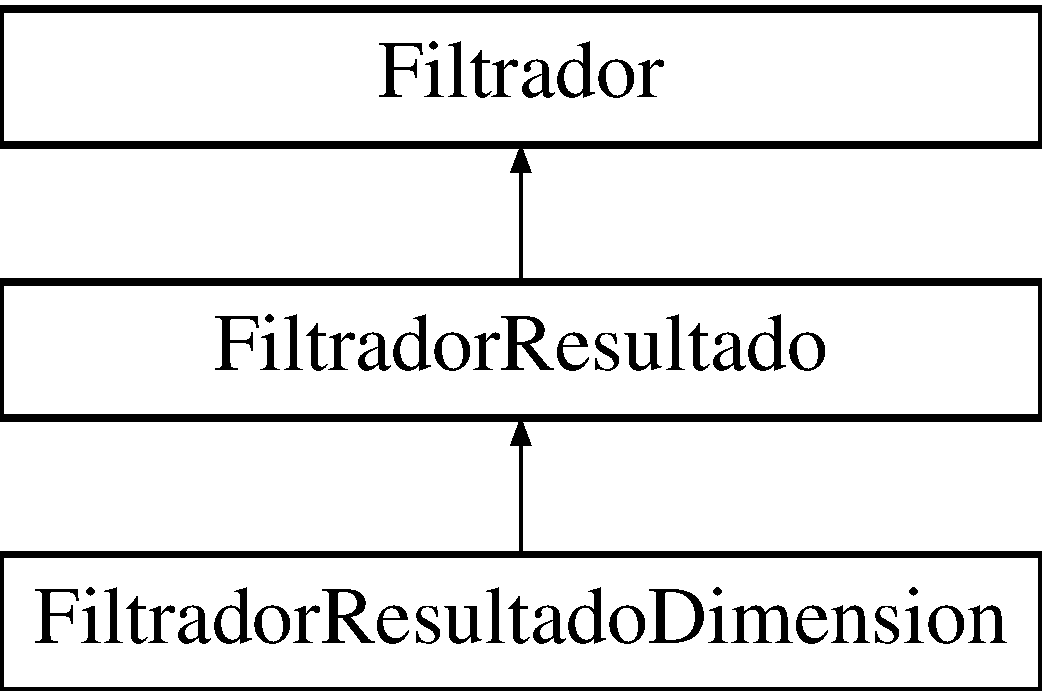
\includegraphics[height=3.000000cm]{classFiltradorResultadoDimension}
\end{center}
\end{figure}
\subsection*{\-Métodos públicos}
\begin{DoxyCompactItemize}
\item 
\hyperlink{classFiltradorResultadoDimension_a40533f3fff8e52b1b4ffe897ef96bab0}{\-Filtrador\-Resultado\-Dimension} (const \-Glib\-::ustring \&resultado)
\item 
virtual \hyperlink{classFiltradorResultadoDimension_aae58c32a57db065571570f6cbea61b59}{$\sim$\-Filtrador\-Resultado\-Dimension} ()
\item 
void \hyperlink{classFiltradorResultadoDimension_a60562082b3ad8788d4f912752093eb09}{filtrar} (\hyperlink{classConsulta}{\-Consulta} \&c)
\end{DoxyCompactItemize}


\subsection{\-Descripción detallada}
\-Resultado de comportamiento \char`\"{}básico\char`\"{}, es decir, no es hecho ni fecha. 

\subsection{\-Documentación del constructor y destructor}
\hypertarget{classFiltradorResultadoDimension_a40533f3fff8e52b1b4ffe897ef96bab0}{\index{\-Filtrador\-Resultado\-Dimension@{\-Filtrador\-Resultado\-Dimension}!\-Filtrador\-Resultado\-Dimension@{\-Filtrador\-Resultado\-Dimension}}
\index{\-Filtrador\-Resultado\-Dimension@{\-Filtrador\-Resultado\-Dimension}!FiltradorResultadoDimension@{\-Filtrador\-Resultado\-Dimension}}
\subsubsection[{\-Filtrador\-Resultado\-Dimension}]{\setlength{\rightskip}{0pt plus 5cm}{\bf \-Filtrador\-Resultado\-Dimension\-::\-Filtrador\-Resultado\-Dimension} (
\begin{DoxyParamCaption}
\item[{const \-Glib\-::ustring \&}]{resultado}
\end{DoxyParamCaption}
)}}\label{classFiltradorResultadoDimension_a40533f3fff8e52b1b4ffe897ef96bab0}
\-Constructor. 
\begin{DoxyParams}{\-Parámetros}
{\em resultado} & nombre del campo \\
\hline
\end{DoxyParams}
\hypertarget{classFiltradorResultadoDimension_aae58c32a57db065571570f6cbea61b59}{\index{\-Filtrador\-Resultado\-Dimension@{\-Filtrador\-Resultado\-Dimension}!$\sim$\-Filtrador\-Resultado\-Dimension@{$\sim$\-Filtrador\-Resultado\-Dimension}}
\index{$\sim$\-Filtrador\-Resultado\-Dimension@{$\sim$\-Filtrador\-Resultado\-Dimension}!FiltradorResultadoDimension@{\-Filtrador\-Resultado\-Dimension}}
\subsubsection[{$\sim$\-Filtrador\-Resultado\-Dimension}]{\setlength{\rightskip}{0pt plus 5cm}{\bf \-Filtrador\-Resultado\-Dimension\-::$\sim$\-Filtrador\-Resultado\-Dimension} (
\begin{DoxyParamCaption}
{}
\end{DoxyParamCaption}
)\hspace{0.3cm}{\ttfamily  \mbox{[}virtual\mbox{]}}}}\label{classFiltradorResultadoDimension_aae58c32a57db065571570f6cbea61b59}
\-Destructor. 

\subsection{\-Documentación de las funciones miembro}
\hypertarget{classFiltradorResultadoDimension_a60562082b3ad8788d4f912752093eb09}{\index{\-Filtrador\-Resultado\-Dimension@{\-Filtrador\-Resultado\-Dimension}!filtrar@{filtrar}}
\index{filtrar@{filtrar}!FiltradorResultadoDimension@{\-Filtrador\-Resultado\-Dimension}}
\subsubsection[{filtrar}]{\setlength{\rightskip}{0pt plus 5cm}void {\bf \-Filtrador\-Resultado\-Dimension\-::filtrar} (
\begin{DoxyParamCaption}
\item[{{\bf \-Consulta} \&}]{c}
\end{DoxyParamCaption}
)\hspace{0.3cm}{\ttfamily  \mbox{[}virtual\mbox{]}}}}\label{classFiltradorResultadoDimension_a60562082b3ad8788d4f912752093eb09}
\-Agrega el resultado a la consulta. 
\begin{DoxyParams}{\-Parámetros}
{\em c} & consulta \\
\hline
\end{DoxyParams}


\-Implementa \hyperlink{classFiltrador_a5c0739dd669ef0de7f2624c77beb14f0}{\-Filtrador}.



\-La documentación para esta clase fue generada a partir de los siguientes ficheros\-:\begin{DoxyCompactItemize}
\item 
cliente/\-Vista/\-Filtrador\-Resultado\-Dimension.\-h\item 
cliente/\-Vista/\-Filtrador\-Resultado\-Dimension.\-cpp\end{DoxyCompactItemize}

\hypertarget{classFiltradorResultadoFecha}{\section{\-Referencia de la \-Clase \-Filtrador\-Resultado\-Fecha}
\label{classFiltradorResultadoFecha}\index{\-Filtrador\-Resultado\-Fecha@{\-Filtrador\-Resultado\-Fecha}}
}


{\ttfamily \#include $<$\-Filtrador\-Resultado\-Fecha.\-h$>$}

\-Diagrama de herencias de \-Filtrador\-Resultado\-Fecha\begin{figure}[H]
\begin{center}
\leavevmode
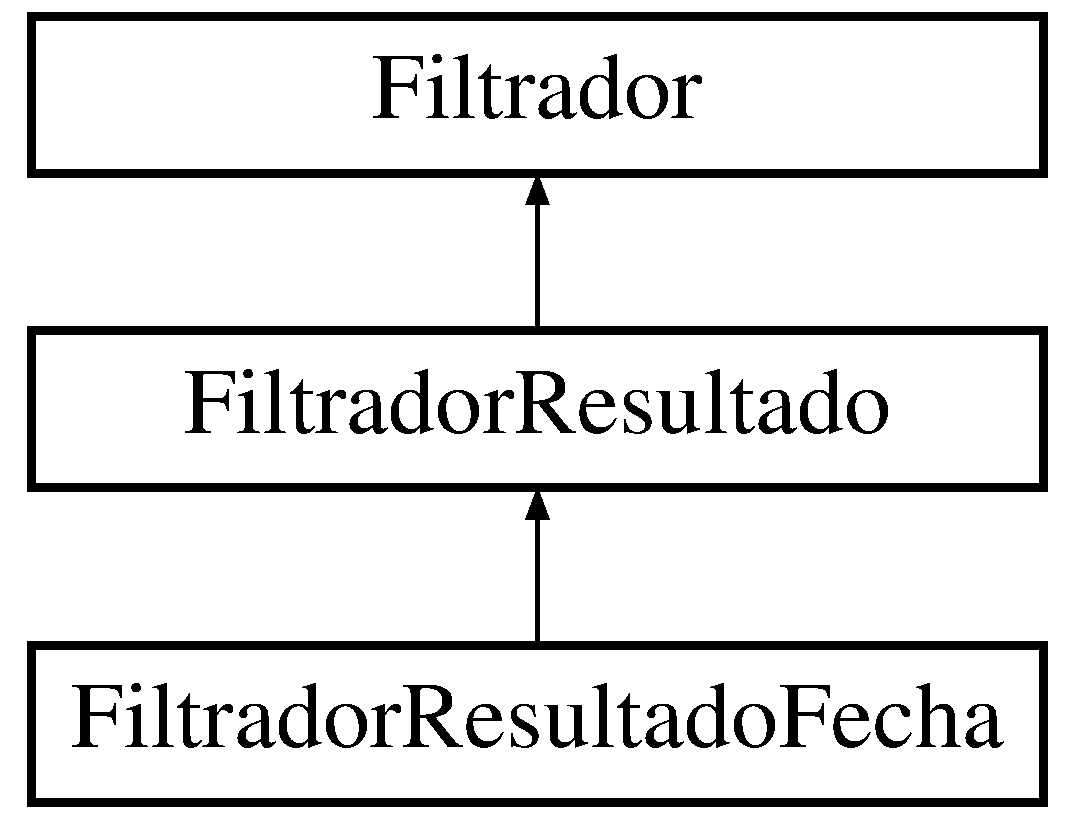
\includegraphics[height=3.000000cm]{classFiltradorResultadoFecha}
\end{center}
\end{figure}
\subsection*{\-Métodos públicos}
\begin{DoxyCompactItemize}
\item 
\hyperlink{classFiltradorResultadoFecha_a709082626c3459d77c1e8a8fe59cea21}{\-Filtrador\-Resultado\-Fecha} (const \-Glib\-::ustring \&fecha, const \-Glib\-::ustring \&valor\-Combo, const \-Glib\-::ustring \&valor\-Entrada)
\item 
virtual \hyperlink{classFiltradorResultadoFecha_a26ac3b00b0ecc7c3a5e88520eb64382d}{$\sim$\-Filtrador\-Resultado\-Fecha} ()
\item 
void \hyperlink{classFiltradorResultadoFecha_a20ed031918bc5f788c8388ab6b26d24c}{filtrar} (\hyperlink{classConsulta}{\-Consulta} \&c)
\end{DoxyCompactItemize}


\subsection{\-Descripción detallada}
\-Resultado de tipo fecha. 

\subsection{\-Documentación del constructor y destructor}
\hypertarget{classFiltradorResultadoFecha_a709082626c3459d77c1e8a8fe59cea21}{\index{\-Filtrador\-Resultado\-Fecha@{\-Filtrador\-Resultado\-Fecha}!\-Filtrador\-Resultado\-Fecha@{\-Filtrador\-Resultado\-Fecha}}
\index{\-Filtrador\-Resultado\-Fecha@{\-Filtrador\-Resultado\-Fecha}!FiltradorResultadoFecha@{\-Filtrador\-Resultado\-Fecha}}
\subsubsection[{\-Filtrador\-Resultado\-Fecha}]{\setlength{\rightskip}{0pt plus 5cm}{\bf \-Filtrador\-Resultado\-Fecha\-::\-Filtrador\-Resultado\-Fecha} (
\begin{DoxyParamCaption}
\item[{const \-Glib\-::ustring \&}]{fecha, }
\item[{const \-Glib\-::ustring \&}]{valor\-Combo, }
\item[{const \-Glib\-::ustring \&}]{valor\-Entrada}
\end{DoxyParamCaption}
)}}\label{classFiltradorResultadoFecha_a709082626c3459d77c1e8a8fe59cea21}
\-Constructor. 
\begin{DoxyParams}{\-Parámetros}
{\em fecha} & nombre del campo \\
\hline
{\em valor\-Combo} & modo de fecha seleccionado \\
\hline
{\em valor\-Entrada} & valor de la entrada de fecha \\
\hline
\end{DoxyParams}
\hypertarget{classFiltradorResultadoFecha_a26ac3b00b0ecc7c3a5e88520eb64382d}{\index{\-Filtrador\-Resultado\-Fecha@{\-Filtrador\-Resultado\-Fecha}!$\sim$\-Filtrador\-Resultado\-Fecha@{$\sim$\-Filtrador\-Resultado\-Fecha}}
\index{$\sim$\-Filtrador\-Resultado\-Fecha@{$\sim$\-Filtrador\-Resultado\-Fecha}!FiltradorResultadoFecha@{\-Filtrador\-Resultado\-Fecha}}
\subsubsection[{$\sim$\-Filtrador\-Resultado\-Fecha}]{\setlength{\rightskip}{0pt plus 5cm}{\bf \-Filtrador\-Resultado\-Fecha\-::$\sim$\-Filtrador\-Resultado\-Fecha} (
\begin{DoxyParamCaption}
{}
\end{DoxyParamCaption}
)\hspace{0.3cm}{\ttfamily  \mbox{[}virtual\mbox{]}}}}\label{classFiltradorResultadoFecha_a26ac3b00b0ecc7c3a5e88520eb64382d}
\-Destructor. 

\subsection{\-Documentación de las funciones miembro}
\hypertarget{classFiltradorResultadoFecha_a20ed031918bc5f788c8388ab6b26d24c}{\index{\-Filtrador\-Resultado\-Fecha@{\-Filtrador\-Resultado\-Fecha}!filtrar@{filtrar}}
\index{filtrar@{filtrar}!FiltradorResultadoFecha@{\-Filtrador\-Resultado\-Fecha}}
\subsubsection[{filtrar}]{\setlength{\rightskip}{0pt plus 5cm}void {\bf \-Filtrador\-Resultado\-Fecha\-::filtrar} (
\begin{DoxyParamCaption}
\item[{{\bf \-Consulta} \&}]{c}
\end{DoxyParamCaption}
)\hspace{0.3cm}{\ttfamily  \mbox{[}virtual\mbox{]}}}}\label{classFiltradorResultadoFecha_a20ed031918bc5f788c8388ab6b26d24c}
\-Agrega el resultado a la consulta. 
\begin{DoxyParams}{\-Parámetros}
{\em c} & consulta \\
\hline
\end{DoxyParams}


\-Implementa \hyperlink{classFiltrador_a5c0739dd669ef0de7f2624c77beb14f0}{\-Filtrador}.



\-La documentación para esta clase fue generada a partir de los siguientes ficheros\-:\begin{DoxyCompactItemize}
\item 
cliente/\-Vista/\-Filtrador\-Resultado\-Fecha.\-h\item 
cliente/\-Vista/\-Filtrador\-Resultado\-Fecha.\-cpp\end{DoxyCompactItemize}

\hypertarget{classFiltradorResultadoHecho}{\section{\-Referencia de la \-Clase \-Filtrador\-Resultado\-Hecho}
\label{classFiltradorResultadoHecho}\index{\-Filtrador\-Resultado\-Hecho@{\-Filtrador\-Resultado\-Hecho}}
}


{\ttfamily \#include $<$\-Filtrador\-Resultado\-Hecho.\-h$>$}

\-Diagrama de herencias de \-Filtrador\-Resultado\-Hecho\begin{figure}[H]
\begin{center}
\leavevmode
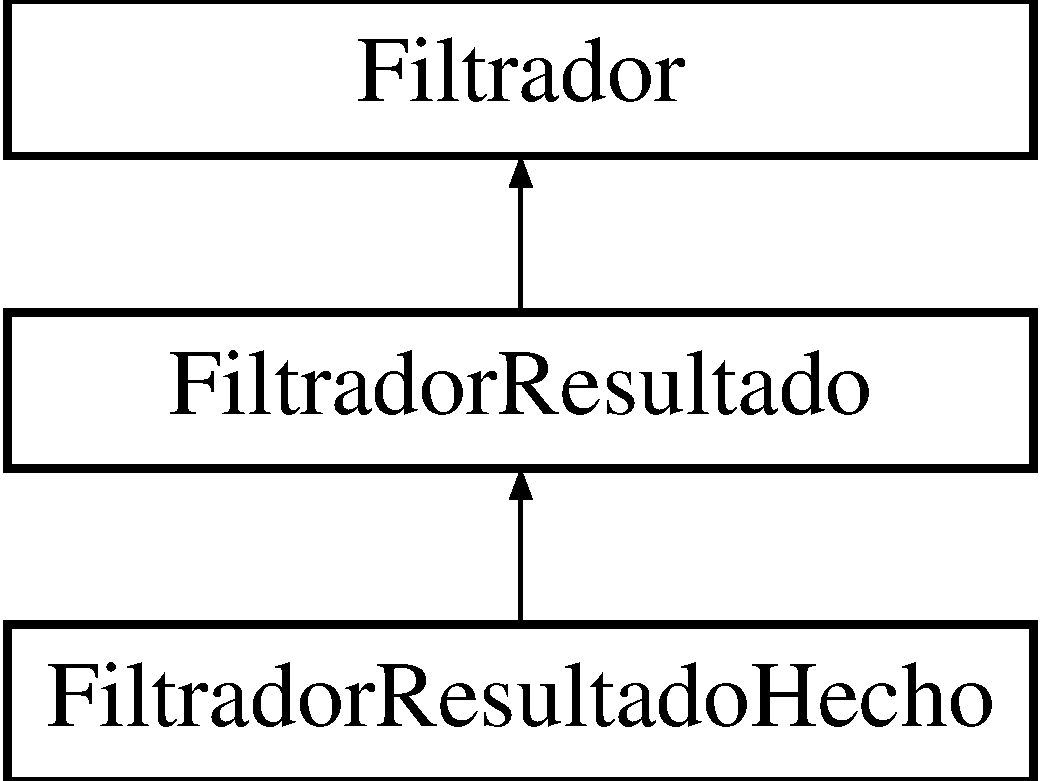
\includegraphics[height=3.000000cm]{classFiltradorResultadoHecho}
\end{center}
\end{figure}
\subsection*{\-Métodos públicos}
\begin{DoxyCompactItemize}
\item 
\hyperlink{classFiltradorResultadoHecho_a9264f0fd7751c390e9c81723525af31b}{\-Filtrador\-Resultado\-Hecho} (const \-Glib\-::ustring \&hecho, const \-Glib\-::ustring \&agregacion)
\item 
virtual \hyperlink{classFiltradorResultadoHecho_add342e2c81ccfdde25f0a1c56599ed8a}{$\sim$\-Filtrador\-Resultado\-Hecho} ()
\item 
void \hyperlink{classFiltradorResultadoHecho_adfcbfa61c6efe4003a7b2170ecc44e59}{filtrar} (\hyperlink{classConsulta}{\-Consulta} \&c)
\end{DoxyCompactItemize}


\subsection{\-Descripción detallada}
\-Resultado de tipo hecho. 

\subsection{\-Documentación del constructor y destructor}
\hypertarget{classFiltradorResultadoHecho_a9264f0fd7751c390e9c81723525af31b}{\index{\-Filtrador\-Resultado\-Hecho@{\-Filtrador\-Resultado\-Hecho}!\-Filtrador\-Resultado\-Hecho@{\-Filtrador\-Resultado\-Hecho}}
\index{\-Filtrador\-Resultado\-Hecho@{\-Filtrador\-Resultado\-Hecho}!FiltradorResultadoHecho@{\-Filtrador\-Resultado\-Hecho}}
\subsubsection[{\-Filtrador\-Resultado\-Hecho}]{\setlength{\rightskip}{0pt plus 5cm}{\bf \-Filtrador\-Resultado\-Hecho\-::\-Filtrador\-Resultado\-Hecho} (
\begin{DoxyParamCaption}
\item[{const \-Glib\-::ustring \&}]{hecho, }
\item[{const \-Glib\-::ustring \&}]{agregacion}
\end{DoxyParamCaption}
)}}\label{classFiltradorResultadoHecho_a9264f0fd7751c390e9c81723525af31b}
\-Constructor. 
\begin{DoxyParams}{\-Parámetros}
{\em hecho} & nombre del campo \\
\hline
{\em agregacion} & nombre de la agregación \\
\hline
\end{DoxyParams}
\hypertarget{classFiltradorResultadoHecho_add342e2c81ccfdde25f0a1c56599ed8a}{\index{\-Filtrador\-Resultado\-Hecho@{\-Filtrador\-Resultado\-Hecho}!$\sim$\-Filtrador\-Resultado\-Hecho@{$\sim$\-Filtrador\-Resultado\-Hecho}}
\index{$\sim$\-Filtrador\-Resultado\-Hecho@{$\sim$\-Filtrador\-Resultado\-Hecho}!FiltradorResultadoHecho@{\-Filtrador\-Resultado\-Hecho}}
\subsubsection[{$\sim$\-Filtrador\-Resultado\-Hecho}]{\setlength{\rightskip}{0pt plus 5cm}{\bf \-Filtrador\-Resultado\-Hecho\-::$\sim$\-Filtrador\-Resultado\-Hecho} (
\begin{DoxyParamCaption}
{}
\end{DoxyParamCaption}
)\hspace{0.3cm}{\ttfamily  \mbox{[}virtual\mbox{]}}}}\label{classFiltradorResultadoHecho_add342e2c81ccfdde25f0a1c56599ed8a}
\-Destructor. 

\subsection{\-Documentación de las funciones miembro}
\hypertarget{classFiltradorResultadoHecho_adfcbfa61c6efe4003a7b2170ecc44e59}{\index{\-Filtrador\-Resultado\-Hecho@{\-Filtrador\-Resultado\-Hecho}!filtrar@{filtrar}}
\index{filtrar@{filtrar}!FiltradorResultadoHecho@{\-Filtrador\-Resultado\-Hecho}}
\subsubsection[{filtrar}]{\setlength{\rightskip}{0pt plus 5cm}void {\bf \-Filtrador\-Resultado\-Hecho\-::filtrar} (
\begin{DoxyParamCaption}
\item[{{\bf \-Consulta} \&}]{c}
\end{DoxyParamCaption}
)\hspace{0.3cm}{\ttfamily  \mbox{[}virtual\mbox{]}}}}\label{classFiltradorResultadoHecho_adfcbfa61c6efe4003a7b2170ecc44e59}
\-Agrega el resultado a la consulta. 
\begin{DoxyParams}{\-Parámetros}
{\em c} & consulta \\
\hline
\end{DoxyParams}


\-Implementa \hyperlink{classFiltrador_a5c0739dd669ef0de7f2624c77beb14f0}{\-Filtrador}.



\-La documentación para esta clase fue generada a partir de los siguientes ficheros\-:\begin{DoxyCompactItemize}
\item 
cliente/\-Vista/\-Filtrador\-Resultado\-Hecho.\-h\item 
cliente/\-Vista/\-Filtrador\-Resultado\-Hecho.\-cpp\end{DoxyCompactItemize}

\hypertarget{classFiltradorSoloDimensionConfigModelo}{\section{\-Referencia de la \-Clase \-Filtrador\-Solo\-Dimension\-Config\-Modelo}
\label{classFiltradorSoloDimensionConfigModelo}\index{\-Filtrador\-Solo\-Dimension\-Config\-Modelo@{\-Filtrador\-Solo\-Dimension\-Config\-Modelo}}
}


{\ttfamily \#include $<$\-Filtrador\-Solo\-Dimension\-Config\-Modelo.\-h$>$}

\-Diagrama de herencias de \-Filtrador\-Solo\-Dimension\-Config\-Modelo\begin{figure}[H]
\begin{center}
\leavevmode
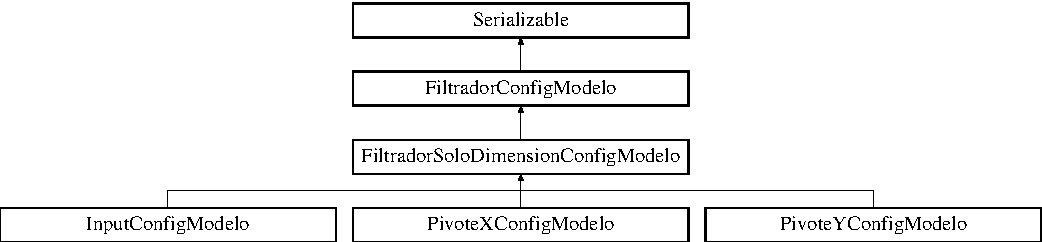
\includegraphics[height=3.246377cm]{classFiltradorSoloDimensionConfigModelo}
\end{center}
\end{figure}
\subsection*{\-Métodos públicos}
\begin{DoxyCompactItemize}
\item 
\hyperlink{classFiltradorSoloDimensionConfigModelo_a65e815f73bbd4d91c1027dd59da86f3f}{\-Filtrador\-Solo\-Dimension\-Config\-Modelo} (unsigned \-I\-D, const std\-::list$<$ std\-::string $>$ \&\-\_\-campos\-Disponibles)
\item 
\hyperlink{classFiltradorSoloDimensionConfigModelo_aa02479e5d24fcdcd65671916026e7f5f}{$\sim$\-Filtrador\-Solo\-Dimension\-Config\-Modelo} ()
\end{DoxyCompactItemize}
\subsection*{\-Métodos protegidos}
\begin{DoxyCompactItemize}
\item 
\hypertarget{classFiltradorSoloDimensionConfigModelo_a0f23a20ad58ab8b45333dcda5a964891}{virtual void {\bfseries completar\-Atributos} ()}\label{classFiltradorSoloDimensionConfigModelo_a0f23a20ad58ab8b45333dcda5a964891}

\end{DoxyCompactItemize}


\subsection{\-Descripción detallada}
\-Clase base para filtradores que sólo tienen una string útil (la que indica qué campo se seleccionó) y se comportan igual en todos los aspectos salvo al momento de construir la consulta. 

\subsection{\-Documentación del constructor y destructor}
\hypertarget{classFiltradorSoloDimensionConfigModelo_a65e815f73bbd4d91c1027dd59da86f3f}{\index{\-Filtrador\-Solo\-Dimension\-Config\-Modelo@{\-Filtrador\-Solo\-Dimension\-Config\-Modelo}!\-Filtrador\-Solo\-Dimension\-Config\-Modelo@{\-Filtrador\-Solo\-Dimension\-Config\-Modelo}}
\index{\-Filtrador\-Solo\-Dimension\-Config\-Modelo@{\-Filtrador\-Solo\-Dimension\-Config\-Modelo}!FiltradorSoloDimensionConfigModelo@{\-Filtrador\-Solo\-Dimension\-Config\-Modelo}}
\subsubsection[{\-Filtrador\-Solo\-Dimension\-Config\-Modelo}]{\setlength{\rightskip}{0pt plus 5cm}{\bf \-Filtrador\-Solo\-Dimension\-Config\-Modelo\-::\-Filtrador\-Solo\-Dimension\-Config\-Modelo} (
\begin{DoxyParamCaption}
\item[{unsigned}]{\-I\-D, }
\item[{const std\-::list$<$ std\-::string $>$ \&}]{\-\_\-campos\-Disponibles}
\end{DoxyParamCaption}
)}}\label{classFiltradorSoloDimensionConfigModelo_a65e815f73bbd4d91c1027dd59da86f3f}
\-Constructor. \hypertarget{classFiltradorSoloDimensionConfigModelo_aa02479e5d24fcdcd65671916026e7f5f}{\index{\-Filtrador\-Solo\-Dimension\-Config\-Modelo@{\-Filtrador\-Solo\-Dimension\-Config\-Modelo}!$\sim$\-Filtrador\-Solo\-Dimension\-Config\-Modelo@{$\sim$\-Filtrador\-Solo\-Dimension\-Config\-Modelo}}
\index{$\sim$\-Filtrador\-Solo\-Dimension\-Config\-Modelo@{$\sim$\-Filtrador\-Solo\-Dimension\-Config\-Modelo}!FiltradorSoloDimensionConfigModelo@{\-Filtrador\-Solo\-Dimension\-Config\-Modelo}}
\subsubsection[{$\sim$\-Filtrador\-Solo\-Dimension\-Config\-Modelo}]{\setlength{\rightskip}{0pt plus 5cm}{\bf \-Filtrador\-Solo\-Dimension\-Config\-Modelo\-::$\sim$\-Filtrador\-Solo\-Dimension\-Config\-Modelo} (
\begin{DoxyParamCaption}
{}
\end{DoxyParamCaption}
)}}\label{classFiltradorSoloDimensionConfigModelo_aa02479e5d24fcdcd65671916026e7f5f}
\-Destructor. 

\-La documentación para esta clase fue generada a partir de los siguientes ficheros\-:\begin{DoxyCompactItemize}
\item 
cliente/\-Modelo/\-Filtrador\-Solo\-Dimension\-Config\-Modelo.\-h\item 
cliente/\-Modelo/\-Filtrador\-Solo\-Dimension\-Config\-Modelo.\-cpp\end{DoxyCompactItemize}

\hypertarget{classFiltroConfigModelo}{\section{\-Referencia de la \-Clase \-Filtro\-Config\-Modelo}
\label{classFiltroConfigModelo}\index{\-Filtro\-Config\-Modelo@{\-Filtro\-Config\-Modelo}}
}


{\ttfamily \#include $<$\-Filtro\-Config\-Modelo.\-h$>$}

\-Diagrama de herencias de \-Filtro\-Config\-Modelo\begin{figure}[H]
\begin{center}
\leavevmode
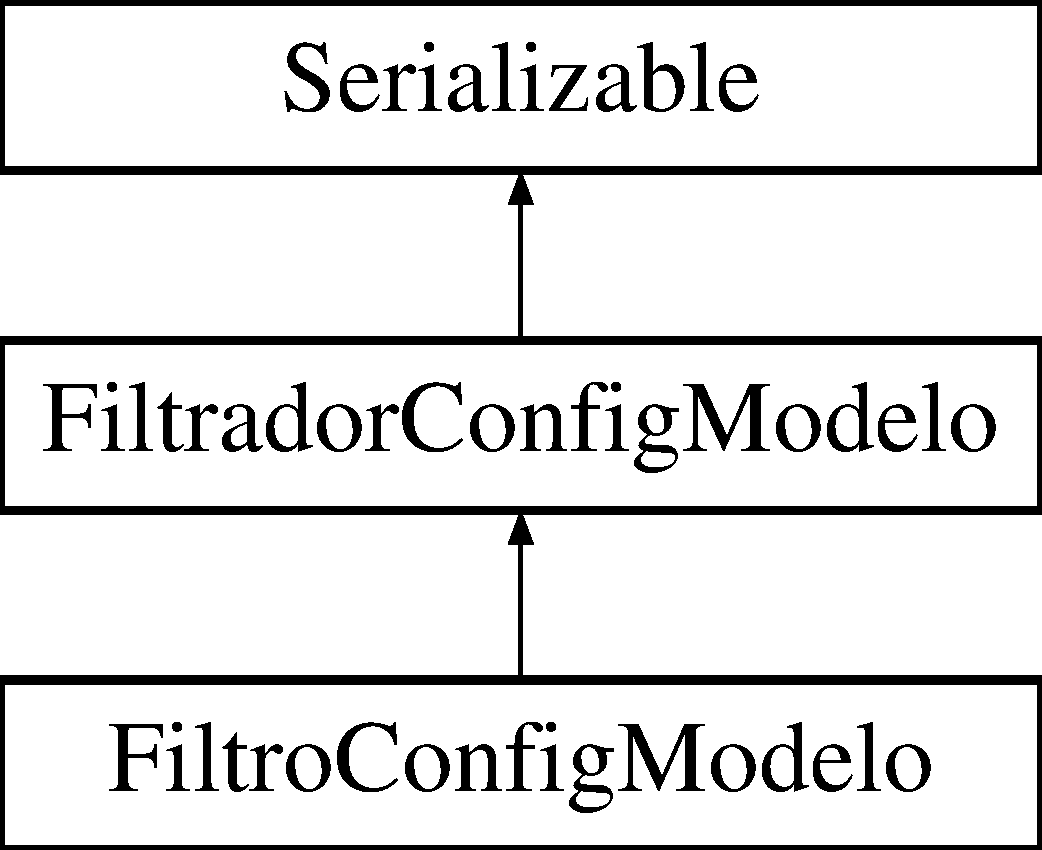
\includegraphics[height=3.000000cm]{classFiltroConfigModelo}
\end{center}
\end{figure}
\subsection*{\-Métodos públicos}
\begin{DoxyCompactItemize}
\item 
\hyperlink{classFiltroConfigModelo_a345f0b72d16ac7b1d971aa18fac11717}{\-Filtro\-Config\-Modelo} (unsigned \-I\-D, const std\-::list$<$ std\-::string $>$ \&campos\-Disponibles)
\item 
\hyperlink{classFiltroConfigModelo_aa0e4383974a930a58f57e5faa92cd845}{$\sim$\-Filtro\-Config\-Modelo} ()
\item 
\hypertarget{classFiltroConfigModelo_a54769347060eeb20fb25137921d7ad36}{void {\bfseries set\-Filtrador\-En} (\hyperlink{classFiltradoresTab}{\-Filtradores\-Tab} $\ast$filt\-Tab)}\label{classFiltroConfigModelo_a54769347060eeb20fb25137921d7ad36}

\item 
\hypertarget{classFiltroConfigModelo_a4cd680914e9fbd4a4d6d66ce6f97ac6b}{void {\bfseries set\-Filtrador\-En} (\hyperlink{classFiltradoresPanel}{\-Filtradores\-Panel} $\ast$filt\-Panel)}\label{classFiltroConfigModelo_a4cd680914e9fbd4a4d6d66ce6f97ac6b}

\end{DoxyCompactItemize}
\subsection*{\-Métodos protegidos}
\begin{DoxyCompactItemize}
\item 
\hypertarget{classFiltroConfigModelo_aa4835820b733580a4f7694f535d89842}{virtual void {\bfseries completar\-Atributos} ()}\label{classFiltroConfigModelo_aa4835820b733580a4f7694f535d89842}

\end{DoxyCompactItemize}


\subsection{\-Descripción detallada}
\-Clase modelo de la configuración de un filtro para una consulta. \-Selecciona campo. \-Si es fecha, puede seleccionar tipo de fecha (mes, bimestre, año, etc.) e ingresar en una \-Gtk\-::\-Entry. \-Si es \hyperlink{classHecho}{\-Hecho}, selecciona mayor, igual o menor y el valor en una \-Gtk\-::\-Entry. \-De otra manera, ingresa en la \-Gtk\-::\-Entry el valor del filtro. 

\subsection{\-Documentación del constructor y destructor}
\hypertarget{classFiltroConfigModelo_a345f0b72d16ac7b1d971aa18fac11717}{\index{\-Filtro\-Config\-Modelo@{\-Filtro\-Config\-Modelo}!\-Filtro\-Config\-Modelo@{\-Filtro\-Config\-Modelo}}
\index{\-Filtro\-Config\-Modelo@{\-Filtro\-Config\-Modelo}!FiltroConfigModelo@{\-Filtro\-Config\-Modelo}}
\subsubsection[{\-Filtro\-Config\-Modelo}]{\setlength{\rightskip}{0pt plus 5cm}{\bf \-Filtro\-Config\-Modelo\-::\-Filtro\-Config\-Modelo} (
\begin{DoxyParamCaption}
\item[{unsigned}]{\-I\-D, }
\item[{const std\-::list$<$ std\-::string $>$ \&}]{campos\-Disponibles}
\end{DoxyParamCaption}
)}}\label{classFiltroConfigModelo_a345f0b72d16ac7b1d971aa18fac11717}
\-Constructor. \hypertarget{classFiltroConfigModelo_aa0e4383974a930a58f57e5faa92cd845}{\index{\-Filtro\-Config\-Modelo@{\-Filtro\-Config\-Modelo}!$\sim$\-Filtro\-Config\-Modelo@{$\sim$\-Filtro\-Config\-Modelo}}
\index{$\sim$\-Filtro\-Config\-Modelo@{$\sim$\-Filtro\-Config\-Modelo}!FiltroConfigModelo@{\-Filtro\-Config\-Modelo}}
\subsubsection[{$\sim$\-Filtro\-Config\-Modelo}]{\setlength{\rightskip}{0pt plus 5cm}{\bf \-Filtro\-Config\-Modelo\-::$\sim$\-Filtro\-Config\-Modelo} (
\begin{DoxyParamCaption}
{}
\end{DoxyParamCaption}
)}}\label{classFiltroConfigModelo_aa0e4383974a930a58f57e5faa92cd845}
\-Destructor. 

\-La documentación para esta clase fue generada a partir de los siguientes ficheros\-:\begin{DoxyCompactItemize}
\item 
cliente/\-Modelo/\-Filtro\-Config\-Modelo.\-h\item 
cliente/\-Modelo/\-Filtro\-Config\-Modelo.\-cpp\end{DoxyCompactItemize}

\hypertarget{classGrafico}{\section{\-Referencia de la \-Clase \-Grafico}
\label{classGrafico}\index{\-Grafico@{\-Grafico}}
}


{\ttfamily \#include $<$\-Grafico.\-h$>$}

\-Diagrama de herencias de \-Grafico\begin{figure}[H]
\begin{center}
\leavevmode
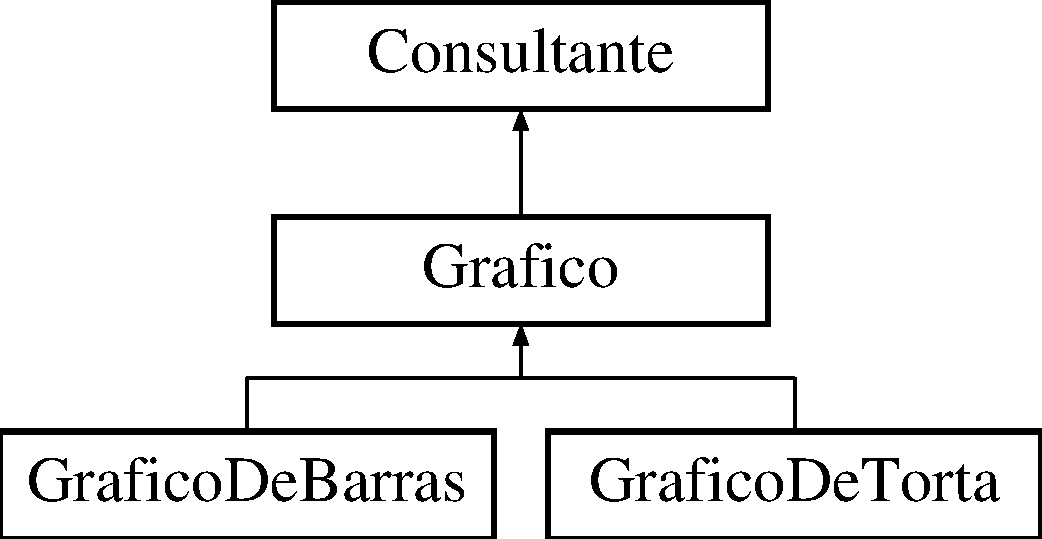
\includegraphics[height=3.000000cm]{classGrafico}
\end{center}
\end{figure}
\subsection*{\-Métodos públicos}
\begin{DoxyCompactItemize}
\item 
\hyperlink{classGrafico_ae432e5a7b909182132551b359a6a1ea3}{\-Grafico} (\hyperlink{classFiltradoresPanel}{\-Filtradores\-Panel} $\ast$f)
\item 
virtual \hyperlink{classGrafico_a1db5d0b80dfa9467542b37278a4f9f66}{$\sim$\-Grafico} ()
\end{DoxyCompactItemize}
\subsection*{\-Métodos protegidos}
\begin{DoxyCompactItemize}
\item 
\hypertarget{classGrafico_a3ea17dc3e92eb867069eab9331891e03}{virtual void {\bfseries hallar\-Normalizacion} (const std\-::list$<$ \hyperlink{classHecho}{\-Hecho} $>$ \&datos)=0}\label{classGrafico_a3ea17dc3e92eb867069eab9331891e03}

\item 
void \hyperlink{classGrafico_a3abd6861308594594d76f09f61087e95}{delete\-Areas} ()
\item 
\hypertarget{classGrafico_a664b44ea30af98769a2c8ba9c07e3743}{void {\bfseries regenerar\-Referencias} ()}\label{classGrafico_a664b44ea30af98769a2c8ba9c07e3743}

\end{DoxyCompactItemize}
\subsection*{\-Atributos protegidos}
\begin{DoxyCompactItemize}
\item 
\hypertarget{classGrafico_a9c1acb54ce5a8c9cd7f11430804467d6}{std\-::list$<$ \hyperlink{classArea}{\-Area} $\ast$ $>$ {\bfseries areas}}\label{classGrafico_a9c1acb54ce5a8c9cd7f11430804467d6}

\item 
\hypertarget{classGrafico_a33c53444bc586899595318a37a0ed16a}{double {\bfseries normalizacion}}\label{classGrafico_a33c53444bc586899595318a37a0ed16a}

\end{DoxyCompactItemize}


\subsection{\-Descripción detallada}
\-Clase abstracta que comprende comportamiento común a un consultante que muestra sus resultados gráficamente. \-Limitado a dos columnas de resultados, el segundo necesariamente un hecho. 

\subsection{\-Documentación del constructor y destructor}
\hypertarget{classGrafico_ae432e5a7b909182132551b359a6a1ea3}{\index{\-Grafico@{\-Grafico}!\-Grafico@{\-Grafico}}
\index{\-Grafico@{\-Grafico}!Grafico@{\-Grafico}}
\subsubsection[{\-Grafico}]{\setlength{\rightskip}{0pt plus 5cm}{\bf \-Grafico\-::\-Grafico} (
\begin{DoxyParamCaption}
\item[{{\bf \-Filtradores\-Panel} $\ast$}]{f}
\end{DoxyParamCaption}
)}}\label{classGrafico_ae432e5a7b909182132551b359a6a1ea3}
\-Constructor. 
\begin{DoxyParams}{\-Parámetros}
{\em f} & filtradores de panel \\
\hline
\end{DoxyParams}
\hypertarget{classGrafico_a1db5d0b80dfa9467542b37278a4f9f66}{\index{\-Grafico@{\-Grafico}!$\sim$\-Grafico@{$\sim$\-Grafico}}
\index{$\sim$\-Grafico@{$\sim$\-Grafico}!Grafico@{\-Grafico}}
\subsubsection[{$\sim$\-Grafico}]{\setlength{\rightskip}{0pt plus 5cm}{\bf \-Grafico\-::$\sim$\-Grafico} (
\begin{DoxyParamCaption}
{}
\end{DoxyParamCaption}
)\hspace{0.3cm}{\ttfamily  \mbox{[}virtual\mbox{]}}}}\label{classGrafico_a1db5d0b80dfa9467542b37278a4f9f66}
\-Destructor. 

\subsection{\-Documentación de las funciones miembro}
\hypertarget{classGrafico_a3abd6861308594594d76f09f61087e95}{\index{\-Grafico@{\-Grafico}!delete\-Areas@{delete\-Areas}}
\index{delete\-Areas@{delete\-Areas}!Grafico@{\-Grafico}}
\subsubsection[{delete\-Areas}]{\setlength{\rightskip}{0pt plus 5cm}void {\bf \-Grafico\-::delete\-Areas} (
\begin{DoxyParamCaption}
{}
\end{DoxyParamCaption}
)\hspace{0.3cm}{\ttfamily  \mbox{[}protected\mbox{]}}}}\label{classGrafico_a3abd6861308594594d76f09f61087e95}
borra y regenera todas las referencias 

\-La documentación para esta clase fue generada a partir de los siguientes ficheros\-:\begin{DoxyCompactItemize}
\item 
cliente/\-Vista/\-Grafico.\-h\item 
cliente/\-Vista/\-Grafico.\-cpp\end{DoxyCompactItemize}

\hypertarget{classGraficoDeBarras}{\section{\-Referencia de la \-Clase \-Grafico\-De\-Barras}
\label{classGraficoDeBarras}\index{\-Grafico\-De\-Barras@{\-Grafico\-De\-Barras}}
}


{\ttfamily \#include $<$\-Grafico\-De\-Barras.\-h$>$}

\-Diagrama de herencias de \-Grafico\-De\-Barras\begin{figure}[H]
\begin{center}
\leavevmode
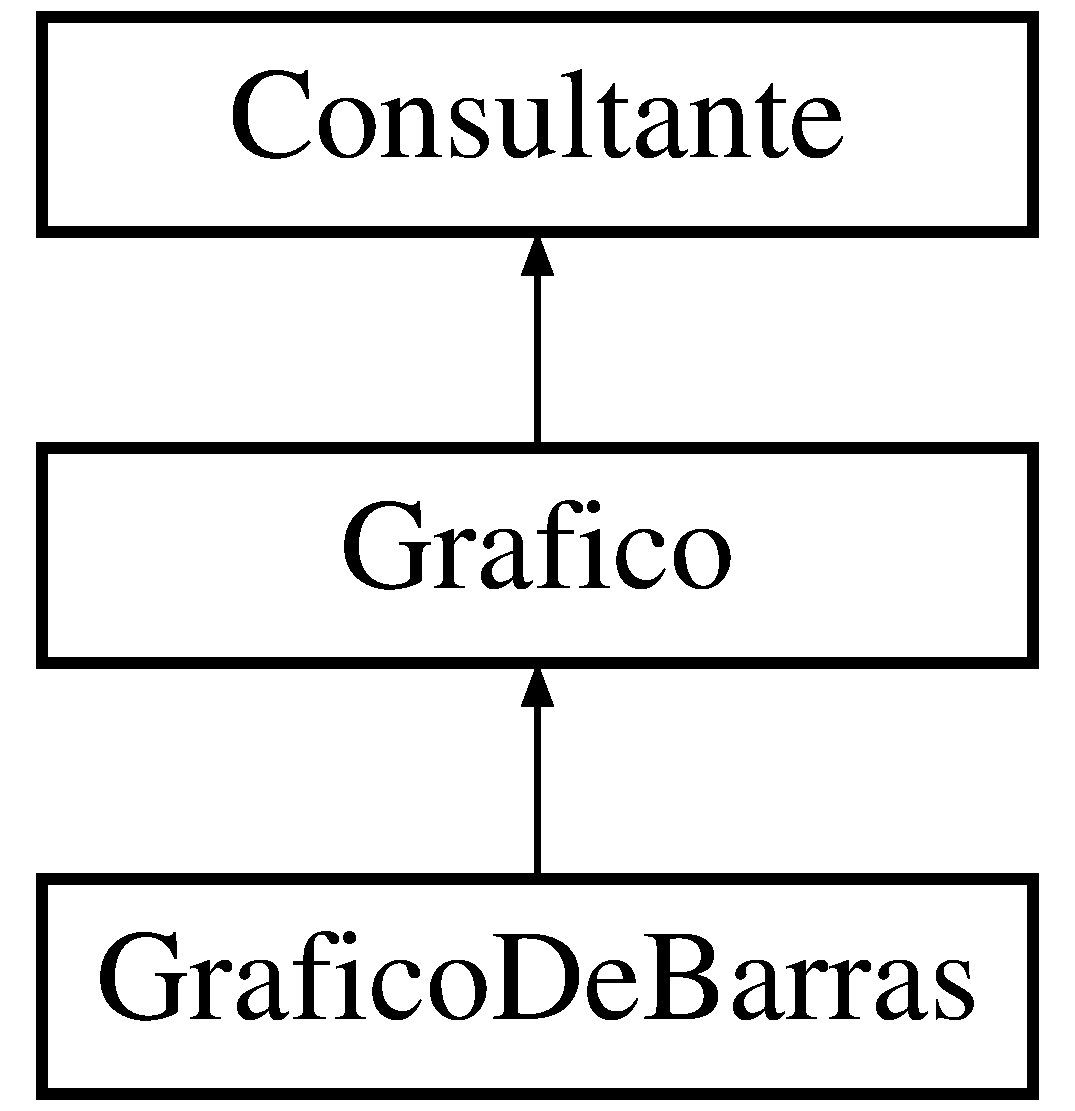
\includegraphics[height=3.000000cm]{classGraficoDeBarras}
\end{center}
\end{figure}
\subsection*{\-Métodos públicos}
\begin{DoxyCompactItemize}
\item 
\hyperlink{classGraficoDeBarras_add802fc700de9e32c48963f63bdbcdaf}{\-Grafico\-De\-Barras} (\hyperlink{classFiltradoresPanel}{\-Filtradores\-Panel} $\ast$f)
\item 
virtual \hyperlink{classGraficoDeBarras_aa00c42c82489d74b8dcb17e636c4a77c}{$\sim$\-Grafico\-De\-Barras} ()
\item 
\hypertarget{classGraficoDeBarras_abfeee8e37ec9ec5dab633747b9ff5b96}{void {\bfseries actualizar\-Datos} (const std\-::list$<$ \hyperlink{classHecho}{\-Hecho} $>$ \&datos)}\label{classGraficoDeBarras_abfeee8e37ec9ec5dab633747b9ff5b96}

\end{DoxyCompactItemize}


\subsection{\-Descripción detallada}
\hyperlink{classConsultante}{\-Consultante} que muestra sus resultados como un gráfico de barras. 

\subsection{\-Documentación del constructor y destructor}
\hypertarget{classGraficoDeBarras_add802fc700de9e32c48963f63bdbcdaf}{\index{\-Grafico\-De\-Barras@{\-Grafico\-De\-Barras}!\-Grafico\-De\-Barras@{\-Grafico\-De\-Barras}}
\index{\-Grafico\-De\-Barras@{\-Grafico\-De\-Barras}!GraficoDeBarras@{\-Grafico\-De\-Barras}}
\subsubsection[{\-Grafico\-De\-Barras}]{\setlength{\rightskip}{0pt plus 5cm}{\bf \-Grafico\-De\-Barras\-::\-Grafico\-De\-Barras} (
\begin{DoxyParamCaption}
\item[{{\bf \-Filtradores\-Panel} $\ast$}]{f}
\end{DoxyParamCaption}
)}}\label{classGraficoDeBarras_add802fc700de9e32c48963f63bdbcdaf}
\-Constructor. 
\begin{DoxyParams}{\-Parámetros}
{\em f} & filtradores del panel \\
\hline
\end{DoxyParams}
\hypertarget{classGraficoDeBarras_aa00c42c82489d74b8dcb17e636c4a77c}{\index{\-Grafico\-De\-Barras@{\-Grafico\-De\-Barras}!$\sim$\-Grafico\-De\-Barras@{$\sim$\-Grafico\-De\-Barras}}
\index{$\sim$\-Grafico\-De\-Barras@{$\sim$\-Grafico\-De\-Barras}!GraficoDeBarras@{\-Grafico\-De\-Barras}}
\subsubsection[{$\sim$\-Grafico\-De\-Barras}]{\setlength{\rightskip}{0pt plus 5cm}{\bf \-Grafico\-De\-Barras\-::$\sim$\-Grafico\-De\-Barras} (
\begin{DoxyParamCaption}
{}
\end{DoxyParamCaption}
)\hspace{0.3cm}{\ttfamily  \mbox{[}virtual\mbox{]}}}}\label{classGraficoDeBarras_aa00c42c82489d74b8dcb17e636c4a77c}
\-Destructor. 

\-La documentación para esta clase fue generada a partir de los siguientes ficheros\-:\begin{DoxyCompactItemize}
\item 
cliente/\-Vista/\-Grafico\-De\-Barras.\-h\item 
cliente/\-Vista/\-Grafico\-De\-Barras.\-cpp\end{DoxyCompactItemize}

\hypertarget{classGraficoDeTorta}{\section{\-Referencia de la \-Clase \-Grafico\-De\-Torta}
\label{classGraficoDeTorta}\index{\-Grafico\-De\-Torta@{\-Grafico\-De\-Torta}}
}


{\ttfamily \#include $<$\-Grafico\-De\-Torta.\-h$>$}

\-Diagrama de herencias de \-Grafico\-De\-Torta\begin{figure}[H]
\begin{center}
\leavevmode
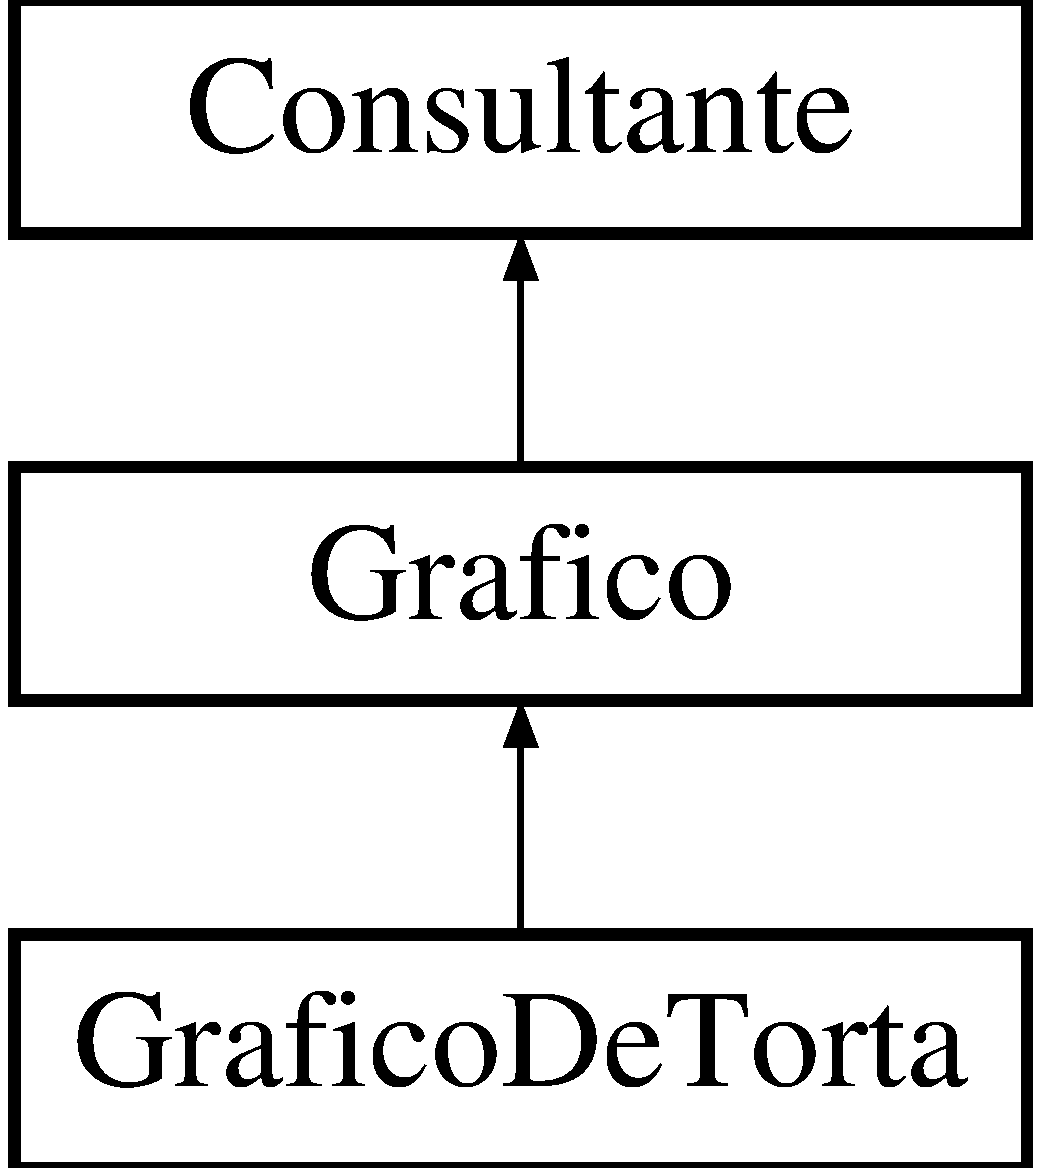
\includegraphics[height=3.000000cm]{classGraficoDeTorta}
\end{center}
\end{figure}
\subsection*{\-Métodos públicos}
\begin{DoxyCompactItemize}
\item 
\hyperlink{classGraficoDeTorta_aabb1e17113cca604d6685fd5d6b0b4be}{\-Grafico\-De\-Torta} (\hyperlink{classFiltradoresPanel}{\-Filtradores\-Panel} $\ast$f)
\item 
virtual \hyperlink{classGraficoDeTorta_acc7233c20887e55613c74dcd5ba26580}{$\sim$\-Grafico\-De\-Torta} ()
\item 
\hypertarget{classGraficoDeTorta_acf701899bc212c273f6ec0db717188c4}{void {\bfseries actualizar\-Datos} (const std\-::list$<$ \hyperlink{classHecho}{\-Hecho} $>$ \&datos)}\label{classGraficoDeTorta_acf701899bc212c273f6ec0db717188c4}

\end{DoxyCompactItemize}


\subsection{\-Descripción detallada}
\hyperlink{classConsultante}{\-Consultante} que muestra sus resultados como un gráfico de torta. 

\subsection{\-Documentación del constructor y destructor}
\hypertarget{classGraficoDeTorta_aabb1e17113cca604d6685fd5d6b0b4be}{\index{\-Grafico\-De\-Torta@{\-Grafico\-De\-Torta}!\-Grafico\-De\-Torta@{\-Grafico\-De\-Torta}}
\index{\-Grafico\-De\-Torta@{\-Grafico\-De\-Torta}!GraficoDeTorta@{\-Grafico\-De\-Torta}}
\subsubsection[{\-Grafico\-De\-Torta}]{\setlength{\rightskip}{0pt plus 5cm}{\bf \-Grafico\-De\-Torta\-::\-Grafico\-De\-Torta} (
\begin{DoxyParamCaption}
\item[{{\bf \-Filtradores\-Panel} $\ast$}]{f}
\end{DoxyParamCaption}
)}}\label{classGraficoDeTorta_aabb1e17113cca604d6685fd5d6b0b4be}
\-Constructor. 
\begin{DoxyParams}{\-Parámetros}
{\em f} & filtradores del panel \\
\hline
\end{DoxyParams}
\hypertarget{classGraficoDeTorta_acc7233c20887e55613c74dcd5ba26580}{\index{\-Grafico\-De\-Torta@{\-Grafico\-De\-Torta}!$\sim$\-Grafico\-De\-Torta@{$\sim$\-Grafico\-De\-Torta}}
\index{$\sim$\-Grafico\-De\-Torta@{$\sim$\-Grafico\-De\-Torta}!GraficoDeTorta@{\-Grafico\-De\-Torta}}
\subsubsection[{$\sim$\-Grafico\-De\-Torta}]{\setlength{\rightskip}{0pt plus 5cm}{\bf \-Grafico\-De\-Torta\-::$\sim$\-Grafico\-De\-Torta} (
\begin{DoxyParamCaption}
{}
\end{DoxyParamCaption}
)\hspace{0.3cm}{\ttfamily  \mbox{[}virtual\mbox{]}}}}\label{classGraficoDeTorta_acc7233c20887e55613c74dcd5ba26580}
\-Destructor. 

\-La documentación para esta clase fue generada a partir de los siguientes ficheros\-:\begin{DoxyCompactItemize}
\item 
cliente/\-Vista/\-Grafico\-De\-Torta.\-h\item 
cliente/\-Vista/\-Grafico\-De\-Torta.\-cpp\end{DoxyCompactItemize}

\hypertarget{classHecho}{\section{\-Referencia de la \-Clase \-Hecho}
\label{classHecho}\index{\-Hecho@{\-Hecho}}
}


{\ttfamily \#include $<$\-Hecho.\-h$>$}

\subsection*{\-Métodos públicos}
\begin{DoxyCompactItemize}
\item 
\hyperlink{classHecho_a7bfac84967a673af43766b925df5d650}{\-Hecho} (const \hyperlink{classHecho}{\-Hecho} \&original)
\item 
\hyperlink{classHecho_a0f6fe75ee75ff640130d431f27a08a00}{\-Hecho} (const \-Glib\-::ustring \&etiqueta, double valor)
\item 
\hyperlink{classHecho_a8536263dce459e232a994ee76462eb6b}{$\sim$\-Hecho} ()
\item 
\hypertarget{classHecho_abf03d7117f1b06dcf962d99e359bd2af}{\hyperlink{classHecho}{\-Hecho} \& {\bfseries operator=} (const \hyperlink{classHecho}{\-Hecho} \&original)}\label{classHecho_abf03d7117f1b06dcf962d99e359bd2af}

\item 
\hypertarget{classHecho_a186f4b322ac31544ae9883f7e5f68558}{const \-Glib\-::ustring \& {\bfseries get\-Etiqueta} () const }\label{classHecho_a186f4b322ac31544ae9883f7e5f68558}

\item 
\hypertarget{classHecho_ab18727b45db7d9726b0dce7adebbfe9a}{double {\bfseries get\-Valor} () const }\label{classHecho_ab18727b45db7d9726b0dce7adebbfe9a}

\end{DoxyCompactItemize}


\subsection{\-Descripción detallada}
\-Encapsula un par $<$ etiqueta, valor $>$. 

\subsection{\-Documentación del constructor y destructor}
\hypertarget{classHecho_a7bfac84967a673af43766b925df5d650}{\index{\-Hecho@{\-Hecho}!\-Hecho@{\-Hecho}}
\index{\-Hecho@{\-Hecho}!Hecho@{\-Hecho}}
\subsubsection[{\-Hecho}]{\setlength{\rightskip}{0pt plus 5cm}{\bf \-Hecho\-::\-Hecho} (
\begin{DoxyParamCaption}
\item[{const {\bf \-Hecho} \&}]{original}
\end{DoxyParamCaption}
)}}\label{classHecho_a7bfac84967a673af43766b925df5d650}
\-Constructor copia. 
\begin{DoxyParams}{\-Parámetros}
{\em original} & el otro \hyperlink{classHecho}{\-Hecho} \\
\hline
\end{DoxyParams}
\hypertarget{classHecho_a0f6fe75ee75ff640130d431f27a08a00}{\index{\-Hecho@{\-Hecho}!\-Hecho@{\-Hecho}}
\index{\-Hecho@{\-Hecho}!Hecho@{\-Hecho}}
\subsubsection[{\-Hecho}]{\setlength{\rightskip}{0pt plus 5cm}{\bf \-Hecho\-::\-Hecho} (
\begin{DoxyParamCaption}
\item[{const \-Glib\-::ustring \&}]{etiqueta, }
\item[{double}]{valor}
\end{DoxyParamCaption}
)}}\label{classHecho_a0f6fe75ee75ff640130d431f27a08a00}
\-Constructor. 
\begin{DoxyParams}{\-Parámetros}
{\em etiqueta} & nombre del dato del área referente \\
\hline
{\em valor} & valor del dato del área referente \\
\hline
\end{DoxyParams}
\hypertarget{classHecho_a8536263dce459e232a994ee76462eb6b}{\index{\-Hecho@{\-Hecho}!$\sim$\-Hecho@{$\sim$\-Hecho}}
\index{$\sim$\-Hecho@{$\sim$\-Hecho}!Hecho@{\-Hecho}}
\subsubsection[{$\sim$\-Hecho}]{\setlength{\rightskip}{0pt plus 5cm}{\bf \-Hecho\-::$\sim$\-Hecho} (
\begin{DoxyParamCaption}
{}
\end{DoxyParamCaption}
)}}\label{classHecho_a8536263dce459e232a994ee76462eb6b}
\-Destructor. 

\-La documentación para esta clase fue generada a partir de los siguientes ficheros\-:\begin{DoxyCompactItemize}
\item 
cliente/\-Vista/\-Hecho.\-h\item 
cliente/\-Vista/\-Hecho.\-cpp\end{DoxyCompactItemize}

\hypertarget{classHilo}{\section{\-Referencia de la \-Clase \-Hilo}
\label{classHilo}\index{\-Hilo@{\-Hilo}}
}


{\ttfamily \#include $<$\-Hilo.\-h$>$}

\-Diagrama de herencias de \-Hilo\begin{figure}[H]
\begin{center}
\leavevmode
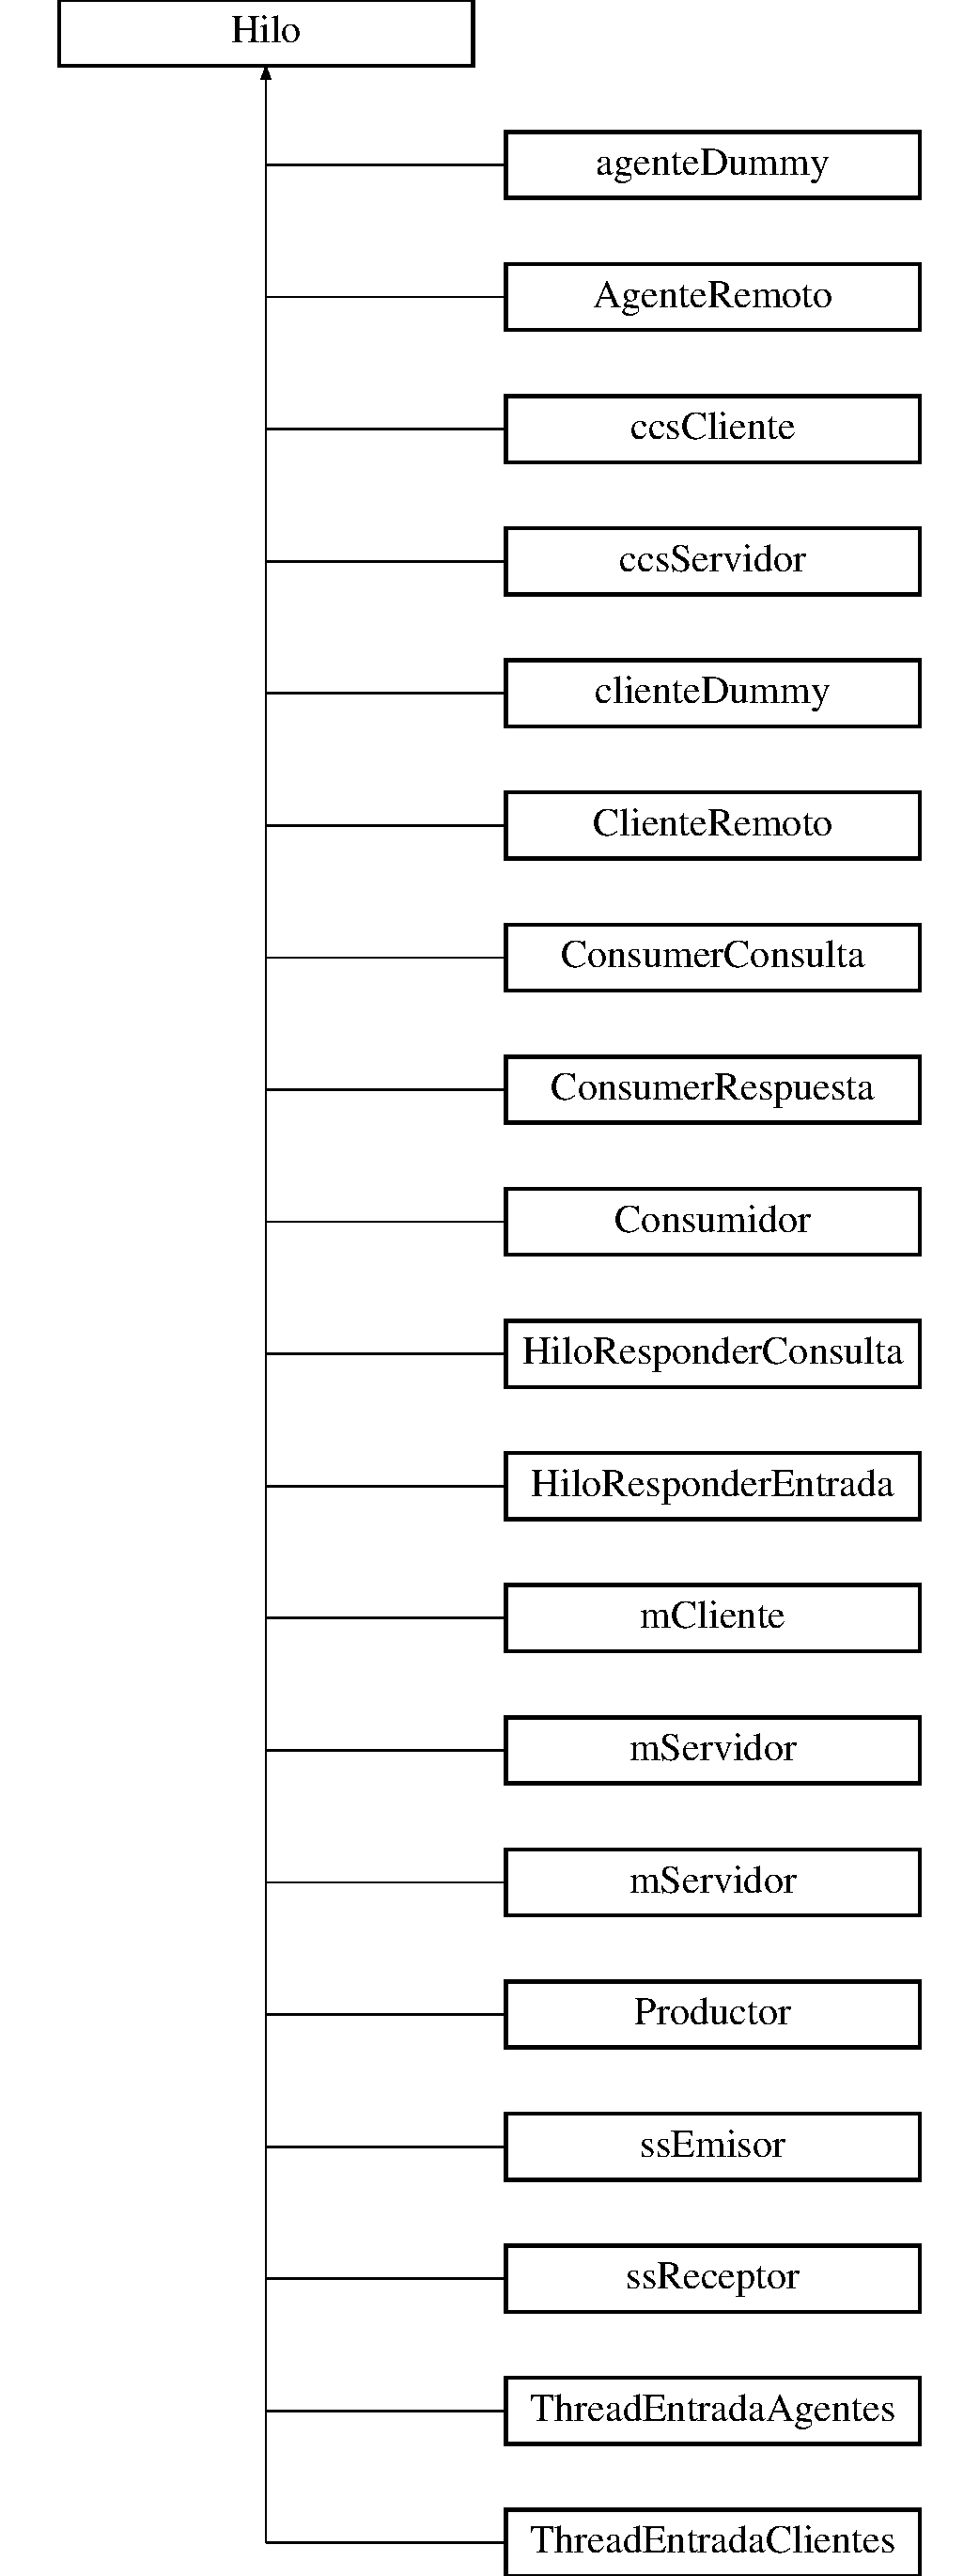
\includegraphics[height=12.000000cm]{classHilo}
\end{center}
\end{figure}
\subsection*{\-Métodos públicos}
\begin{DoxyCompactItemize}
\item 
\hypertarget{classHilo_a509c256ad0af1b7e4322757d502566b2}{\hyperlink{classHilo_a509c256ad0af1b7e4322757d502566b2}{\-Hilo} ()}\label{classHilo_a509c256ad0af1b7e4322757d502566b2}

\begin{DoxyCompactList}\small\item\em \-Constructor sin argumentos de hilo. \end{DoxyCompactList}\item 
\hypertarget{classHilo_a55cb0cf0942900ab24a5622745b743db}{virtual \hyperlink{classHilo_a55cb0cf0942900ab24a5622745b743db}{$\sim$\-Hilo} ()}\label{classHilo_a55cb0cf0942900ab24a5622745b743db}

\begin{DoxyCompactList}\small\item\em \-Destructor de \hyperlink{classHilo}{\-Hilo}. \end{DoxyCompactList}\item 
\hypertarget{classHilo_ad430a6ca9db5339d53a3bdcd4d0e96e9}{virtual void \hyperlink{classHilo_ad430a6ca9db5339d53a3bdcd4d0e96e9}{iniciar} ()}\label{classHilo_ad430a6ca9db5339d53a3bdcd4d0e96e9}

\begin{DoxyCompactList}\small\item\em \-Metodo que inicia la ejecucion del hilo. \end{DoxyCompactList}\item 
\hypertarget{classHilo_ae631df24234346f7c0899cc2c33eb017}{virtual void \hyperlink{classHilo_ae631df24234346f7c0899cc2c33eb017}{parar} ()}\label{classHilo_ae631df24234346f7c0899cc2c33eb017}

\begin{DoxyCompactList}\small\item\em \-Metodo que pone al hilo en estado de detener la ejecucion. \end{DoxyCompactList}\item 
\hypertarget{classHilo_a187b055e3504487a6bb64340fac2c70d}{virtual void \hyperlink{classHilo_a187b055e3504487a6bb64340fac2c70d}{correr} ()=0}\label{classHilo_a187b055e3504487a6bb64340fac2c70d}

\begin{DoxyCompactList}\small\item\em \-Metodo virtual puro, que corre cuando se ejecuta el hilo. \end{DoxyCompactList}\item 
\hypertarget{classHilo_a0d929d8f8783060a040966c91466025c}{virtual void \hyperlink{classHilo_a0d929d8f8783060a040966c91466025c}{sincronizar} ()}\label{classHilo_a0d929d8f8783060a040966c91466025c}

\begin{DoxyCompactList}\small\item\em \-Metodo que espera a que finalice el hilo. \end{DoxyCompactList}\item 
\hypertarget{classHilo_a8aee7c83c953aebc358b9628eb80dd91}{bool \hyperlink{classHilo_a8aee7c83c953aebc358b9628eb80dd91}{corriendo} ()}\label{classHilo_a8aee7c83c953aebc358b9628eb80dd91}

\begin{DoxyCompactList}\small\item\em \-Metodo retornado true si el hilo esta corriendo o si esta listo para correr. \end{DoxyCompactList}\item 
\hypertarget{classHilo_a246e81bf78d664fabf0c4fe96feab550}{bool \hyperlink{classHilo_a246e81bf78d664fabf0c4fe96feab550}{sincronizado} ()}\label{classHilo_a246e81bf78d664fabf0c4fe96feab550}

\begin{DoxyCompactList}\small\item\em \-Retorna un bool indicando si el \hyperlink{classHilo}{\-Hilo} a sido sincronizado. \end{DoxyCompactList}\end{DoxyCompactItemize}


\subsection{\-Descripción detallada}
\-Clase \-Abstracta que utilizada para manipular un \hyperlink{classHilo}{\-Hilo}. 

\-La documentación para esta clase fue generada a partir de los siguientes ficheros\-:\begin{DoxyCompactItemize}
\item 
comun/\-Hilo.\-h\item 
comun/\-Hilo.\-cpp\end{DoxyCompactItemize}

\hypertarget{classHiloResponderConsulta}{\section{\-Referencia de la \-Clase \-Hilo\-Responder\-Consulta}
\label{classHiloResponderConsulta}\index{\-Hilo\-Responder\-Consulta@{\-Hilo\-Responder\-Consulta}}
}


{\ttfamily \#include $<$\-Hilo\-Responder\-Consulta.\-h$>$}

\-Diagrama de herencias de \-Hilo\-Responder\-Consulta\begin{figure}[H]
\begin{center}
\leavevmode
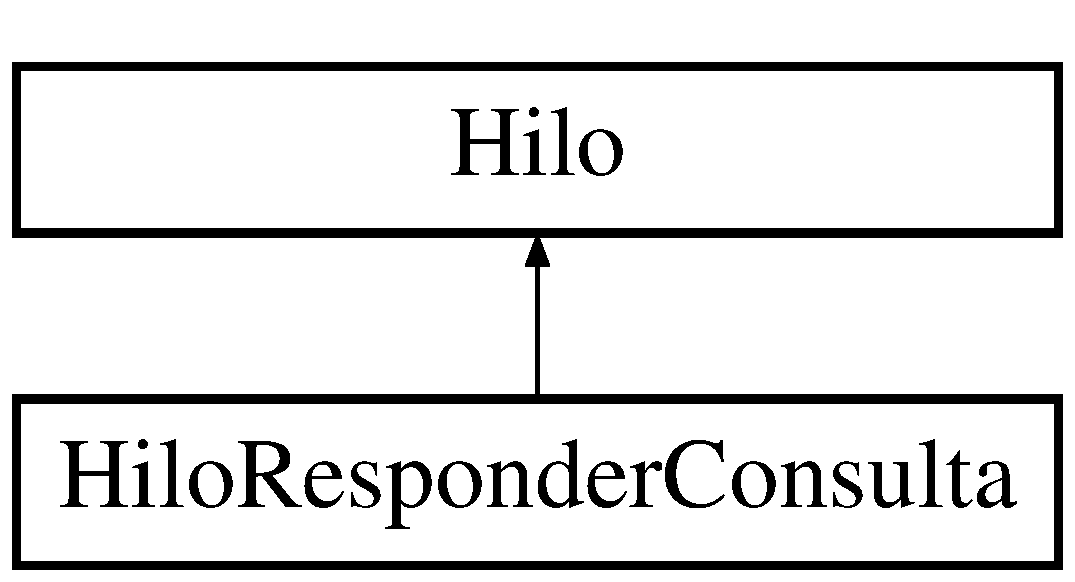
\includegraphics[height=2.000000cm]{classHiloResponderConsulta}
\end{center}
\end{figure}
\subsection*{\-Métodos públicos}
\begin{DoxyCompactItemize}
\item 
\hyperlink{classHiloResponderConsulta_aef65ff26b3d1ece048e2a83038e4a891}{\-Hilo\-Responder\-Consulta} (\hyperlink{classBLQueue}{\-Consultas\-Clientes\-Servidor} \&cconsultas, \hyperlink{classResolvedorConsultas}{\-Resolvedor\-Consultas} \&rcons)
\item 
\hyperlink{classHiloResponderConsulta_a460be54bcc8b8e6236a7c292192d56d4}{$\sim$\-Hilo\-Responder\-Consulta} ()
\item 
void \hyperlink{classHiloResponderConsulta_a11e5fc2a5b3ae20696a1051a4c282845}{correr} ()
\end{DoxyCompactItemize}


\subsection{\-Descripción detallada}
\-Es la clase encargada de la resolución de consultas del cliente. \-Es una clase heredera de hilo que hace las de consumer de la cola de consultas del servidor. \-A su vez, se encarga de enviar la consulta a través del socket del cliente requerido. 

\subsection{\-Documentación del constructor y destructor}
\hypertarget{classHiloResponderConsulta_aef65ff26b3d1ece048e2a83038e4a891}{\index{\-Hilo\-Responder\-Consulta@{\-Hilo\-Responder\-Consulta}!\-Hilo\-Responder\-Consulta@{\-Hilo\-Responder\-Consulta}}
\index{\-Hilo\-Responder\-Consulta@{\-Hilo\-Responder\-Consulta}!HiloResponderConsulta@{\-Hilo\-Responder\-Consulta}}
\subsubsection[{\-Hilo\-Responder\-Consulta}]{\setlength{\rightskip}{0pt plus 5cm}{\bf \-Hilo\-Responder\-Consulta\-::\-Hilo\-Responder\-Consulta} (
\begin{DoxyParamCaption}
\item[{{\bf \-Consultas\-Clientes\-Servidor} \&}]{cconsultas, }
\item[{{\bf \-Resolvedor\-Consultas} \&}]{rcons}
\end{DoxyParamCaption}
)}}\label{classHiloResponderConsulta_aef65ff26b3d1ece048e2a83038e4a891}
\-Constructor de \-Hilo\-Responderconsulta. 
\begin{DoxyParams}{\-Parámetros}
{\em cconsultas} & \-Cola de consultas del servidor. \-Debe ser bloqueante y thread safe. \\
\hline
\end{DoxyParams}
\begin{DoxySeeAlso}{\-Ver también}
\hyperlink{classBLQueue}{\-B\-L\-Queue} 
\end{DoxySeeAlso}

\begin{DoxyParams}{\-Parámetros}
{\em rcons} & \-Objeto capaz de resolver una consulta. \\
\hline
\end{DoxyParams}
\hypertarget{classHiloResponderConsulta_a460be54bcc8b8e6236a7c292192d56d4}{\index{\-Hilo\-Responder\-Consulta@{\-Hilo\-Responder\-Consulta}!$\sim$\-Hilo\-Responder\-Consulta@{$\sim$\-Hilo\-Responder\-Consulta}}
\index{$\sim$\-Hilo\-Responder\-Consulta@{$\sim$\-Hilo\-Responder\-Consulta}!HiloResponderConsulta@{\-Hilo\-Responder\-Consulta}}
\subsubsection[{$\sim$\-Hilo\-Responder\-Consulta}]{\setlength{\rightskip}{0pt plus 5cm}{\bf \-Hilo\-Responder\-Consulta\-::$\sim$\-Hilo\-Responder\-Consulta} (
\begin{DoxyParamCaption}
{}
\end{DoxyParamCaption}
)}}\label{classHiloResponderConsulta_a460be54bcc8b8e6236a7c292192d56d4}
\-Destructor. \-Si esta corriendo, lo detiene. 

\subsection{\-Documentación de las funciones miembro}
\hypertarget{classHiloResponderConsulta_a11e5fc2a5b3ae20696a1051a4c282845}{\index{\-Hilo\-Responder\-Consulta@{\-Hilo\-Responder\-Consulta}!correr@{correr}}
\index{correr@{correr}!HiloResponderConsulta@{\-Hilo\-Responder\-Consulta}}
\subsubsection[{correr}]{\setlength{\rightskip}{0pt plus 5cm}void {\bf \-Hilo\-Responder\-Consulta\-::correr} (
\begin{DoxyParamCaption}
{}
\end{DoxyParamCaption}
)\hspace{0.3cm}{\ttfamily  \mbox{[}virtual\mbox{]}}}}\label{classHiloResponderConsulta_a11e5fc2a5b3ae20696a1051a4c282845}
\-Es el metodo llamado por el callback del hilo. \-Es el encargado de sacar consultas de la cola, pedir la respuesta y enviarla a través del \hyperlink{classClienteRemoto}{\-Cliente\-Remoto} correspondiente. 

\-Implementa \hyperlink{classHilo_a187b055e3504487a6bb64340fac2c70d}{\-Hilo}.



\-La documentación para esta clase fue generada a partir de los siguientes ficheros\-:\begin{DoxyCompactItemize}
\item 
servidor/servidor/\-Hilo\-Responder\-Consulta.\-h\item 
servidor/servidor/\-Hilo\-Responder\-Consulta.\-cpp\end{DoxyCompactItemize}

\hypertarget{classHiloResponderEntrada}{\section{\-Referencia de la \-Clase \-Hilo\-Responder\-Entrada}
\label{classHiloResponderEntrada}\index{\-Hilo\-Responder\-Entrada@{\-Hilo\-Responder\-Entrada}}
}


{\ttfamily \#include $<$\-Hilo\-Responder\-Entrada.\-h$>$}

\-Diagrama de herencias de \-Hilo\-Responder\-Entrada\begin{figure}[H]
\begin{center}
\leavevmode
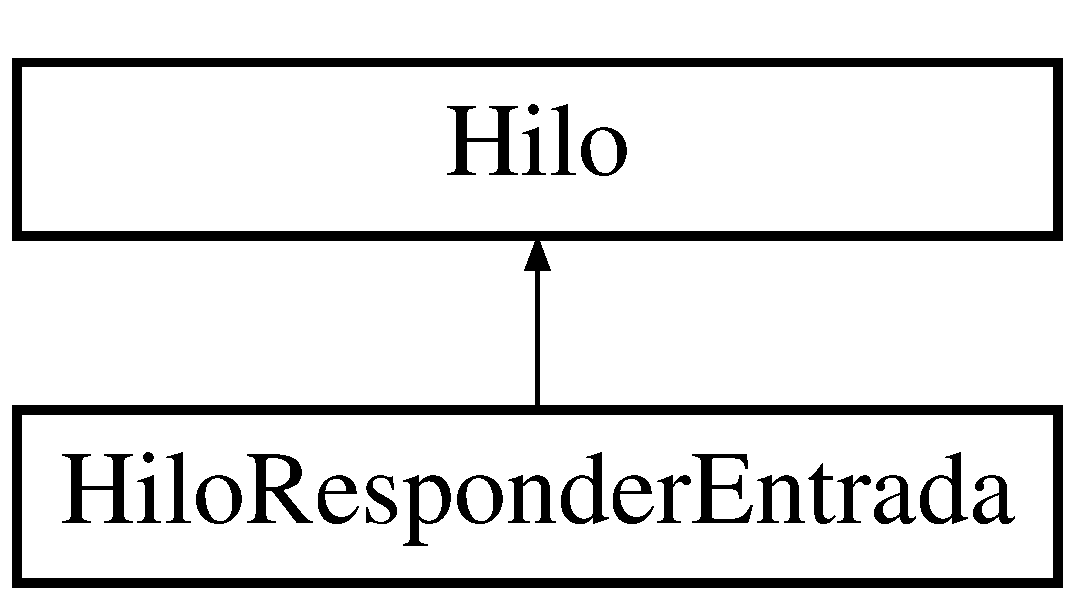
\includegraphics[height=2.000000cm]{classHiloResponderEntrada}
\end{center}
\end{figure}
\subsection*{\-Métodos públicos}
\begin{DoxyCompactItemize}
\item 
\hyperlink{classHiloResponderEntrada_a119af6408470efacfd792ad0bed927e3}{\-Hilo\-Responder\-Entrada} (\hyperlink{classBLQueue}{\-Consultas\-Agentes\-Servidor} \&cconsultas, \hyperlink{classResolvedorEntradas}{\-Resolvedor\-Entradas} \&rentr)
\item 
\hyperlink{classHiloResponderEntrada_af4930fabd3f5a9fd45132bb8ff8a1981}{$\sim$\-Hilo\-Responder\-Entrada} ()
\item 
void \hyperlink{classHiloResponderEntrada_afb23d9181ce6bb9e5ceff8e2394c4518}{correr} ()
\end{DoxyCompactItemize}


\subsection{\-Descripción detallada}
\-Es la clase encargada de la resolución de entradas del agente. \-Es una clase heredera de hilo que hace las de consumer de la cola de entradas del servidor. \-A su vez, se encarga de enviar la respuestas a través del socket del agente pertinente. 

\subsection{\-Documentación del constructor y destructor}
\hypertarget{classHiloResponderEntrada_a119af6408470efacfd792ad0bed927e3}{\index{\-Hilo\-Responder\-Entrada@{\-Hilo\-Responder\-Entrada}!\-Hilo\-Responder\-Entrada@{\-Hilo\-Responder\-Entrada}}
\index{\-Hilo\-Responder\-Entrada@{\-Hilo\-Responder\-Entrada}!HiloResponderEntrada@{\-Hilo\-Responder\-Entrada}}
\subsubsection[{\-Hilo\-Responder\-Entrada}]{\setlength{\rightskip}{0pt plus 5cm}{\bf \-Hilo\-Responder\-Entrada\-::\-Hilo\-Responder\-Entrada} (
\begin{DoxyParamCaption}
\item[{{\bf \-Consultas\-Agentes\-Servidor} \&}]{cconsultas, }
\item[{{\bf \-Resolvedor\-Entradas} \&}]{rentr}
\end{DoxyParamCaption}
)}}\label{classHiloResponderEntrada_a119af6408470efacfd792ad0bed927e3}
\-Constructor de \hyperlink{classHiloResponderEntrada}{\-Hilo\-Responder\-Entrada}. 
\begin{DoxyParams}{\-Parámetros}
{\em cconsultas} & \hyperlink{classReferencia}{\-Referencia} a la cola de entradas del servidor. \-Debe ser bloqueante y thread safe. \\
\hline
\end{DoxyParams}
\begin{DoxySeeAlso}{\-Ver también}
\hyperlink{classBLQueue}{\-B\-L\-Queue} 
\end{DoxySeeAlso}

\begin{DoxyParams}{\-Parámetros}
{\em rentr} & \-Objeto capaz de resolver entradas. \\
\hline
\end{DoxyParams}
\hypertarget{classHiloResponderEntrada_af4930fabd3f5a9fd45132bb8ff8a1981}{\index{\-Hilo\-Responder\-Entrada@{\-Hilo\-Responder\-Entrada}!$\sim$\-Hilo\-Responder\-Entrada@{$\sim$\-Hilo\-Responder\-Entrada}}
\index{$\sim$\-Hilo\-Responder\-Entrada@{$\sim$\-Hilo\-Responder\-Entrada}!HiloResponderEntrada@{\-Hilo\-Responder\-Entrada}}
\subsubsection[{$\sim$\-Hilo\-Responder\-Entrada}]{\setlength{\rightskip}{0pt plus 5cm}{\bf \-Hilo\-Responder\-Entrada\-::$\sim$\-Hilo\-Responder\-Entrada} (
\begin{DoxyParamCaption}
{}
\end{DoxyParamCaption}
)}}\label{classHiloResponderEntrada_af4930fabd3f5a9fd45132bb8ff8a1981}
\-Destructor. \-Si esta corriendo, detiene la ejecucion del hilo. 

\subsection{\-Documentación de las funciones miembro}
\hypertarget{classHiloResponderEntrada_afb23d9181ce6bb9e5ceff8e2394c4518}{\index{\-Hilo\-Responder\-Entrada@{\-Hilo\-Responder\-Entrada}!correr@{correr}}
\index{correr@{correr}!HiloResponderEntrada@{\-Hilo\-Responder\-Entrada}}
\subsubsection[{correr}]{\setlength{\rightskip}{0pt plus 5cm}void {\bf \-Hilo\-Responder\-Entrada\-::correr} (
\begin{DoxyParamCaption}
{}
\end{DoxyParamCaption}
)\hspace{0.3cm}{\ttfamily  \mbox{[}virtual\mbox{]}}}}\label{classHiloResponderEntrada_afb23d9181ce6bb9e5ceff8e2394c4518}
\-Es el método llamado por el callback del hilo. \-Es el encargado de sacar consultas de la cola, pedir la respuesta y enviarla a traves del \hyperlink{classAgenteRemoto}{\-Agente\-Remoto} correspondiente. 

\-Implementa \hyperlink{classHilo_a187b055e3504487a6bb64340fac2c70d}{\-Hilo}.



\-La documentación para esta clase fue generada a partir de los siguientes ficheros\-:\begin{DoxyCompactItemize}
\item 
servidor/servidor/\-Hilo\-Responder\-Entrada.\-h\item 
servidor/servidor/\-Hilo\-Responder\-Entrada.\-cpp\end{DoxyCompactItemize}

\hypertarget{classIndice}{\section{\-Referencia de la plantilla de la \-Clase \-Indice$<$ \-\_\-dato\-\_\- $>$}
\label{classIndice}\index{\-Indice$<$ \-\_\-dato\-\_\- $>$@{\-Indice$<$ \-\_\-dato\-\_\- $>$}}
}


{\ttfamily \#include $<$\-Indice.\-hpp$>$}

\subsection*{\-Tipos públicos}
\begin{DoxyCompactItemize}
\item 
\hypertarget{classIndice_abf092d7caf818f0723c052909eb5997c}{typedef std\-::multimap$<$ \-\_\-dato\-\_\-, \*
\-Id\-\_\-\-Registro $>$ {\bfseries \-Mapa}}\label{classIndice_abf092d7caf818f0723c052909eb5997c}

\item 
\hypertarget{classIndice_a9b5f40892f2626ec60fdbc5e0cdd852d}{typedef \-Mapa\-::iterator {\bfseries \-Iterador}}\label{classIndice_a9b5f40892f2626ec60fdbc5e0cdd852d}

\item 
\hypertarget{classIndice_a86759fbc9a5288d56f80a53aa5a2d0c8}{typedef std\-::pair$<$ \-Iterador, \*
\-Iterador $>$ {\bfseries \-Rango}}\label{classIndice_a86759fbc9a5288d56f80a53aa5a2d0c8}

\end{DoxyCompactItemize}
\subsection*{\-Métodos públicos}
\begin{DoxyCompactItemize}
\item 
\hypertarget{classIndice_a82ef9133b088853d57985113629af828}{\hyperlink{classIndice_a82ef9133b088853d57985113629af828}{\-Indice} ()}\label{classIndice_a82ef9133b088853d57985113629af828}

\begin{DoxyCompactList}\small\item\em \-Constructor sin argumentos. \end{DoxyCompactList}\item 
\-Lista\-\_\-\-Id \hyperlink{classIndice_afdf3110afeff5365dba38626271de7b3}{recuperar} (\-\_\-dato\-\_\- dato)
\begin{DoxyCompactList}\small\item\em \-Recupera una \-Lista de \-Ids que corresponde al valor \char`\"{}dato\char`\"{}. \end{DoxyCompactList}\item 
void \hyperlink{classIndice_a03931620413b48005812abce76a8990b}{recuperar} (\-\_\-dato\-\_\- dato, \-Lista\-\_\-\-Id \&lista)
\begin{DoxyCompactList}\small\item\em \-Recupera una \-Lista de \-Ids que corresponde al valor \char`\"{}dato\char`\"{}. \end{DoxyCompactList}\item 
void \hyperlink{classIndice_aedf78836fd9be8256b03409138cb87fd}{agregar} (\-\_\-dato\-\_\- dato, \-Id\-\_\-\-Registro registro)
\begin{DoxyCompactList}\small\item\em \-Recupera una \-Lista de \-Ids que corresponde al valor \char`\"{}dato\char`\"{}. \end{DoxyCompactList}\item 
\hypertarget{classIndice_ad0c1c1247847d11d37615aa00f52e1dd}{void \hyperlink{classIndice_ad0c1c1247847d11d37615aa00f52e1dd}{limpiar} ()}\label{classIndice_ad0c1c1247847d11d37615aa00f52e1dd}

\begin{DoxyCompactList}\small\item\em \-Se borra y restablece el contenido del indice. \end{DoxyCompactList}\end{DoxyCompactItemize}


\subsection{\-Descripción detallada}
\subsubsection*{template$<$class \-\_\-dato\-\_\-$>$class Indice$<$ \-\_\-dato\-\_\- $>$}

\-Esta clase es un templete creada para funcionar como indice, que guarda los id de registros para un valores del tipo \-\_\-dato\-\_\-. 

\subsection{\-Documentación de las funciones miembro}
\hypertarget{classIndice_aedf78836fd9be8256b03409138cb87fd}{\index{\-Indice@{\-Indice}!agregar@{agregar}}
\index{agregar@{agregar}!Indice@{\-Indice}}
\subsubsection[{agregar}]{\setlength{\rightskip}{0pt plus 5cm}template$<$class \-\_\-dato\-\_\-$>$ void {\bf \-Indice}$<$ \-\_\-dato\-\_\- $>$\-::{\bf agregar} (
\begin{DoxyParamCaption}
\item[{\-\_\-dato\-\_\-}]{dato, }
\item[{\-Id\-\_\-\-Registro}]{registro}
\end{DoxyParamCaption}
)\hspace{0.3cm}{\ttfamily  \mbox{[}inline\mbox{]}}}}\label{classIndice_aedf78836fd9be8256b03409138cb87fd}


\-Recupera una \-Lista de \-Ids que corresponde al valor \char`\"{}dato\char`\"{}. 


\begin{DoxyParams}{\-Parámetros}
{\em dato} & valor que se guardara en el indice. \\
\hline
{\em registro} & id del registro para el cual se guardara el dato \\
\hline
\end{DoxyParams}
\hypertarget{classIndice_afdf3110afeff5365dba38626271de7b3}{\index{\-Indice@{\-Indice}!recuperar@{recuperar}}
\index{recuperar@{recuperar}!Indice@{\-Indice}}
\subsubsection[{recuperar}]{\setlength{\rightskip}{0pt plus 5cm}template$<$class \-\_\-dato\-\_\-$>$ \-Lista\-\_\-\-Id {\bf \-Indice}$<$ \-\_\-dato\-\_\- $>$\-::{\bf recuperar} (
\begin{DoxyParamCaption}
\item[{\-\_\-dato\-\_\-}]{dato}
\end{DoxyParamCaption}
)\hspace{0.3cm}{\ttfamily  \mbox{[}inline\mbox{]}}}}\label{classIndice_afdf3110afeff5365dba38626271de7b3}


\-Recupera una \-Lista de \-Ids que corresponde al valor \char`\"{}dato\char`\"{}. 


\begin{DoxyParams}{\-Parámetros}
{\em dato} & valor del cual se va a recuperar la lista de ids \\
\hline
\end{DoxyParams}
\begin{DoxyReturn}{\-Devuelve}
lista que contiene los ids recuperados 
\end{DoxyReturn}
\hypertarget{classIndice_a03931620413b48005812abce76a8990b}{\index{\-Indice@{\-Indice}!recuperar@{recuperar}}
\index{recuperar@{recuperar}!Indice@{\-Indice}}
\subsubsection[{recuperar}]{\setlength{\rightskip}{0pt plus 5cm}template$<$class \-\_\-dato\-\_\-$>$ void {\bf \-Indice}$<$ \-\_\-dato\-\_\- $>$\-::{\bf recuperar} (
\begin{DoxyParamCaption}
\item[{\-\_\-dato\-\_\-}]{dato, }
\item[{\-Lista\-\_\-\-Id \&}]{lista}
\end{DoxyParamCaption}
)\hspace{0.3cm}{\ttfamily  \mbox{[}inline\mbox{]}}}}\label{classIndice_a03931620413b48005812abce76a8990b}


\-Recupera una \-Lista de \-Ids que corresponde al valor \char`\"{}dato\char`\"{}. 


\begin{DoxyParams}{\-Parámetros}
{\em dato} & valor del cual se va a recuperar la lista de ids. \\
\hline
{\em lista} & es la lista donde se almacenaran los ids recuperados \\
\hline
\end{DoxyParams}


\-La documentación para esta clase fue generada a partir del siguiente fichero\-:\begin{DoxyCompactItemize}
\item 
servidor/\-Motor\-De\-Consultas/\-Indice.\-hpp\end{DoxyCompactItemize}

\hypertarget{classIndiceDeFechas}{\section{\-Referencia de la \-Clase \-Indice\-De\-Fechas}
\label{classIndiceDeFechas}\index{\-Indice\-De\-Fechas@{\-Indice\-De\-Fechas}}
}


{\ttfamily \#include $<$\-Indice\-De\-Fechas.\-h$>$}

\subsection*{\-Métodos públicos}
\begin{DoxyCompactItemize}
\item 
\hypertarget{classIndiceDeFechas_adbb24ea96af6412784ed12b547035bfa}{\hyperlink{classIndiceDeFechas_adbb24ea96af6412784ed12b547035bfa}{\-Indice\-De\-Fechas} ()}\label{classIndiceDeFechas_adbb24ea96af6412784ed12b547035bfa}

\begin{DoxyCompactList}\small\item\em \-Constructor sin argumentos. \end{DoxyCompactList}\item 
void \hyperlink{classIndiceDeFechas_a3ea1d6d6c6a57a8a53dea9b8adf86468}{recuperar} (const \-Fecha \&fecha, \-Lista\-\_\-\-Id \&ids) const 
\begin{DoxyCompactList}\small\item\em \-Se recupera una lista con \-Ids que corresponden a la fecha pasada como argumento. \end{DoxyCompactList}\item 
void \hyperlink{classIndiceDeFechas_a35d827e4bdd41c60fbb60fb100894292}{guardar\-Fecha} (const \-Fecha \&fecha, const \-Id\-\_\-\-Registro \&id)
\begin{DoxyCompactList}\small\item\em \-Se guarda una fecha al indice con su id correspondiente. \end{DoxyCompactList}\item 
\hypertarget{classIndiceDeFechas_a27f43bb41937c43900ce29bce09a8131}{void \hyperlink{classIndiceDeFechas_a27f43bb41937c43900ce29bce09a8131}{limpiar} ()}\label{classIndiceDeFechas_a27f43bb41937c43900ce29bce09a8131}

\begin{DoxyCompactList}\small\item\em \-Se borra y reestablece el contenido del indice. \end{DoxyCompactList}\end{DoxyCompactItemize}


\subsection{\-Descripción detallada}
\-Esta clase es la encargada de funcionar como un indice para las fechas, guardando los id de registros, permitiendo que los ids sean recuperados por distintos tipos de rangos para las fechas. 

\subsection{\-Documentación de las funciones miembro}
\hypertarget{classIndiceDeFechas_a35d827e4bdd41c60fbb60fb100894292}{\index{\-Indice\-De\-Fechas@{\-Indice\-De\-Fechas}!guardar\-Fecha@{guardar\-Fecha}}
\index{guardar\-Fecha@{guardar\-Fecha}!IndiceDeFechas@{\-Indice\-De\-Fechas}}
\subsubsection[{guardar\-Fecha}]{\setlength{\rightskip}{0pt plus 5cm}void {\bf \-Indice\-De\-Fechas\-::guardar\-Fecha} (
\begin{DoxyParamCaption}
\item[{const \-Fecha \&}]{fecha, }
\item[{const \-Id\-\_\-\-Registro \&}]{id}
\end{DoxyParamCaption}
)}}\label{classIndiceDeFechas_a35d827e4bdd41c60fbb60fb100894292}


\-Se guarda una fecha al indice con su id correspondiente. 


\begin{DoxyParams}{\-Parámetros}
{\em fecha} & valor de fecha por que se va a guardar en el indice \\
\hline
{\em id} & identificador de la fecha \\
\hline
\end{DoxyParams}
\hypertarget{classIndiceDeFechas_a3ea1d6d6c6a57a8a53dea9b8adf86468}{\index{\-Indice\-De\-Fechas@{\-Indice\-De\-Fechas}!recuperar@{recuperar}}
\index{recuperar@{recuperar}!IndiceDeFechas@{\-Indice\-De\-Fechas}}
\subsubsection[{recuperar}]{\setlength{\rightskip}{0pt plus 5cm}void {\bf \-Indice\-De\-Fechas\-::recuperar} (
\begin{DoxyParamCaption}
\item[{const \-Fecha \&}]{fecha, }
\item[{\-Lista\-\_\-\-Id \&}]{ids}
\end{DoxyParamCaption}
) const}}\label{classIndiceDeFechas_a3ea1d6d6c6a57a8a53dea9b8adf86468}


\-Se recupera una lista con \-Ids que corresponden a la fecha pasada como argumento. 


\begin{DoxyParams}{\-Parámetros}
{\em fecha} & valor por el cual se van a recupara los ids \\
\hline
\end{DoxyParams}
\begin{DoxyReturn}{\-Devuelve}
lista que contiene los ids recuperados \-Se recupera una lista con \-Ids que corresponden a la fecha pasada como argumento. 
\end{DoxyReturn}

\begin{DoxyParams}{\-Parámetros}
{\em fecha} & valor por el cual se van a recupara los ids \\
\hline
{\em ids} & lista donde se guardaran los ids recuperados \\
\hline
\end{DoxyParams}


\-La documentación para esta clase fue generada a partir de los siguientes ficheros\-:\begin{DoxyCompactItemize}
\item 
servidor/\-Motor\-De\-Consultas/\-Indice\-De\-Fechas.\-h\item 
servidor/\-Motor\-De\-Consultas/\-Indice\-De\-Fechas.\-cpp\end{DoxyCompactItemize}

\hypertarget{classInputConfigModelo}{\section{\-Referencia de la \-Clase \-Input\-Config\-Modelo}
\label{classInputConfigModelo}\index{\-Input\-Config\-Modelo@{\-Input\-Config\-Modelo}}
}


{\ttfamily \#include $<$\-Input\-Config\-Modelo.\-h$>$}

\-Diagrama de herencias de \-Input\-Config\-Modelo\begin{figure}[H]
\begin{center}
\leavevmode
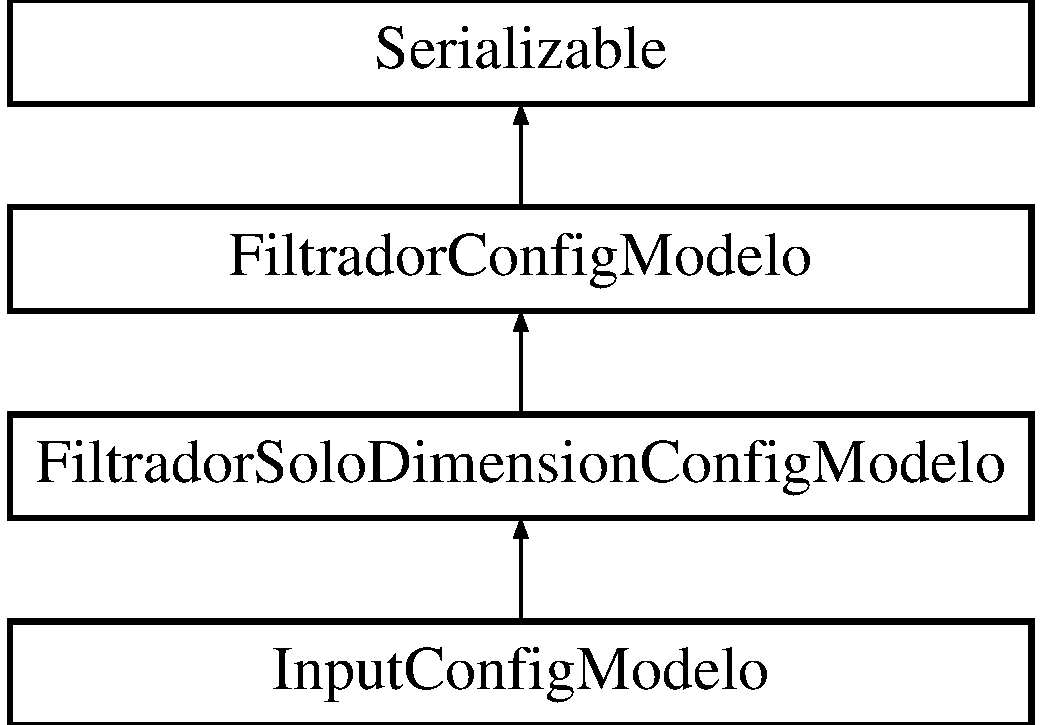
\includegraphics[height=4.000000cm]{classInputConfigModelo}
\end{center}
\end{figure}
\subsection*{\-Métodos públicos}
\begin{DoxyCompactItemize}
\item 
\hyperlink{classInputConfigModelo_a3c8191f6e7738641b7979df02ece471a}{\-Input\-Config\-Modelo} (unsigned \-I\-D, const std\-::list$<$ std\-::string $>$ \&\-\_\-campos\-Disponibles)
\item 
\hyperlink{classInputConfigModelo_a3a81ac4a041230e82e1a7bf42776dc5d}{$\sim$\-Input\-Config\-Modelo} ()
\item 
\hypertarget{classInputConfigModelo_ab217433ebe10462ad3faf554361af5e3}{void {\bfseries set\-Filtrador\-En} (\hyperlink{classFiltradoresTab}{\-Filtradores\-Tab} $\ast$filt\-Tab)}\label{classInputConfigModelo_ab217433ebe10462ad3faf554361af5e3}

\item 
\hypertarget{classInputConfigModelo_a3b00ce24fba77b1b5823099d1624c53d}{void {\bfseries set\-Filtrador\-En} (\hyperlink{classFiltradoresPanel}{\-Filtradores\-Panel} $\ast$filt\-Panel)}\label{classInputConfigModelo_a3b00ce24fba77b1b5823099d1624c53d}

\end{DoxyCompactItemize}


\subsection{\-Descripción detallada}
\-Clase que modela la configuración de un input para una consulta. \-Sólo selecciona el campo. 

\subsection{\-Documentación del constructor y destructor}
\hypertarget{classInputConfigModelo_a3c8191f6e7738641b7979df02ece471a}{\index{\-Input\-Config\-Modelo@{\-Input\-Config\-Modelo}!\-Input\-Config\-Modelo@{\-Input\-Config\-Modelo}}
\index{\-Input\-Config\-Modelo@{\-Input\-Config\-Modelo}!InputConfigModelo@{\-Input\-Config\-Modelo}}
\subsubsection[{\-Input\-Config\-Modelo}]{\setlength{\rightskip}{0pt plus 5cm}{\bf \-Input\-Config\-Modelo\-::\-Input\-Config\-Modelo} (
\begin{DoxyParamCaption}
\item[{unsigned}]{\-I\-D, }
\item[{const std\-::list$<$ std\-::string $>$ \&}]{\-\_\-campos\-Disponibles}
\end{DoxyParamCaption}
)}}\label{classInputConfigModelo_a3c8191f6e7738641b7979df02ece471a}
\-Constructor. \hypertarget{classInputConfigModelo_a3a81ac4a041230e82e1a7bf42776dc5d}{\index{\-Input\-Config\-Modelo@{\-Input\-Config\-Modelo}!$\sim$\-Input\-Config\-Modelo@{$\sim$\-Input\-Config\-Modelo}}
\index{$\sim$\-Input\-Config\-Modelo@{$\sim$\-Input\-Config\-Modelo}!InputConfigModelo@{\-Input\-Config\-Modelo}}
\subsubsection[{$\sim$\-Input\-Config\-Modelo}]{\setlength{\rightskip}{0pt plus 5cm}{\bf \-Input\-Config\-Modelo\-::$\sim$\-Input\-Config\-Modelo} (
\begin{DoxyParamCaption}
{}
\end{DoxyParamCaption}
)}}\label{classInputConfigModelo_a3a81ac4a041230e82e1a7bf42776dc5d}
\-Destructor. 

\-La documentación para esta clase fue generada a partir de los siguientes ficheros\-:\begin{DoxyCompactItemize}
\item 
cliente/\-Modelo/\-Input\-Config\-Modelo.\-h\item 
cliente/\-Modelo/\-Input\-Config\-Modelo.\-cpp\end{DoxyCompactItemize}

\hypertarget{classLock}{\section{\-Referencia de la \-Clase \-Lock}
\label{classLock}\index{\-Lock@{\-Lock}}
}


{\ttfamily \#include $<$\-Mutex.\-h$>$}

\subsection*{\-Métodos públicos}
\begin{DoxyCompactItemize}
\item 
\hypertarget{classLock_a2c786576eddddb484a6a02a7dea52904}{{\bfseries \-Lock} (\hyperlink{classMutex}{\-Mutex} \&m)}\label{classLock_a2c786576eddddb484a6a02a7dea52904}

\end{DoxyCompactItemize}


\subsection{\-Descripción detallada}
\-Clase que aplica un patron \-R\-A\-I\-I para manejo cómodo de \hyperlink{classMutex}{\-Mutex}. 

\-La documentación para esta clase fue generada a partir del siguiente fichero\-:\begin{DoxyCompactItemize}
\item 
comun/\-Mutex.\-h\end{DoxyCompactItemize}

\hypertarget{classM__Fechas}{\section{\-Referencia de la \-Clase \-M\-\_\-\-Fechas}
\label{classM__Fechas}\index{\-M\-\_\-\-Fechas@{\-M\-\_\-\-Fechas}}
}


{\ttfamily \#include $<$\-M\-\_\-\-Fechas.\-h$>$}

\subsection*{\-Métodos públicos}
\begin{DoxyCompactItemize}
\item 
\hypertarget{classM__Fechas_a4e85392938b64b9e75860de17ce9e954}{\hyperlink{classM__Fechas_a4e85392938b64b9e75860de17ce9e954}{\-M\-\_\-\-Fechas} ()}\label{classM__Fechas_a4e85392938b64b9e75860de17ce9e954}

\begin{DoxyCompactList}\small\item\em \-Constructor sin argumentos. \end{DoxyCompactList}\item 
\-Fecha \hyperlink{classM__Fechas_a9ab0eddea3638aba66d48215c216d91e}{fecha} (const std\-::string \&fecha\-Comun) const 
\item 
\hypertarget{classM__Fechas_ac343493066e728100dfeb386d247d808}{bool {\bfseries es\-Fecha\-Convecional} (const std\-::string \&\hyperlink{classM__Fechas_a9ab0eddea3638aba66d48215c216d91e}{fecha}) const }\label{classM__Fechas_ac343493066e728100dfeb386d247d808}

\item 
\-Fecha \hyperlink{classM__Fechas_a549b5b7c70620d16f24623ab6c0a7ec6}{rango} (const \-Fecha \&f1, const \-Fecha \&f2) const 
\begin{DoxyCompactList}\small\item\em \-Transforma dos \-Fechas en una \-Fecha \-Compuesta, que representa un rango de fechas. \end{DoxyCompactList}\item 
\-Fecha \hyperlink{classM__Fechas_a1d302c89571ae873947a636de221ae0d}{fecha} (int dia, int \hyperlink{classM__Fechas_ae6ad20c72a5f70a334613da72459c006}{mes}, int \hyperlink{classM__Fechas_a833db0292ef2aae8764fb1e4d397dbfb}{anio}) const 
\begin{DoxyCompactList}\small\item\em \-Transforma una fecha a partir de de los datos numericos de esta, al formato utilizado en la aplicacion. \end{DoxyCompactList}\item 
\-Fecha \hyperlink{classM__Fechas_a833db0292ef2aae8764fb1e4d397dbfb}{anio} (const std\-::string \&\hyperlink{classM__Fechas_a833db0292ef2aae8764fb1e4d397dbfb}{anio}) const 
\begin{DoxyCompactList}\small\item\em \-A partir de un año se crea un \-Fecha \-Rango que corresponde a todo el año. \-Que compredera las fechas comprendidas en ese periodo. \end{DoxyCompactList}\item 
\-Fecha \hyperlink{classM__Fechas_a1b1343d9bf9d4fdd62bffbfc1ddb55ba}{semestre} (int sem, const std\-::string \&\hyperlink{classM__Fechas_a833db0292ef2aae8764fb1e4d397dbfb}{anio}) const 
\begin{DoxyCompactList}\small\item\em \-A partir de un año y un semestre se crea una \-Fecha de \-Rango. \-Que compredera las fechas comprendidas en ese periodo. \end{DoxyCompactList}\item 
\-Fecha \hyperlink{classM__Fechas_ac900ccecd850f4d01fd9c6a0a26549e4}{cuatrimestre} (int cuat, const std\-::string \&\hyperlink{classM__Fechas_a833db0292ef2aae8764fb1e4d397dbfb}{anio}) const 
\begin{DoxyCompactList}\small\item\em \-A partir de un año y un cuatrimestre se crea una \-Fecha de \-Rango. \-Que compredera las fechas comprendidas en ese periodo. \end{DoxyCompactList}\item 
\-Fecha \hyperlink{classM__Fechas_a26b592cebfd7ac3a1965937961bbe731}{trimestre} (int tri, const std\-::string \&\hyperlink{classM__Fechas_a833db0292ef2aae8764fb1e4d397dbfb}{anio}) const 
\begin{DoxyCompactList}\small\item\em \-A partir de un año y un trimestre se crea una \-Fecha de \-Rango. \-Que compredera las fechas comprendidas en ese periodo. \end{DoxyCompactList}\item 
\-Fecha \hyperlink{classM__Fechas_ae22a1174bdcacf0fd15c1a437e85b701}{bimestre} (int bim, const std\-::string \&\hyperlink{classM__Fechas_a833db0292ef2aae8764fb1e4d397dbfb}{anio}) const 
\begin{DoxyCompactList}\small\item\em \-A partir de un año y un bimestre se crea una \-Fecha de \-Rango. \-Que compredera las fechas comprendidas en ese periodo. \end{DoxyCompactList}\item 
\-Fecha \hyperlink{classM__Fechas_ae6ad20c72a5f70a334613da72459c006}{mes} (int \hyperlink{classM__Fechas_ae6ad20c72a5f70a334613da72459c006}{mes}, const std\-::string \&\hyperlink{classM__Fechas_a833db0292ef2aae8764fb1e4d397dbfb}{anio}) const 
\begin{DoxyCompactList}\small\item\em \-A partir de un año y un mes se crea una \-Fecha de \-Rango. \-Que compredera las fechas comprendidas en ese periodo. \end{DoxyCompactList}\item 
\-Fecha \hyperlink{classM__Fechas_a32fe27a2628bce51a3762ce8bc3e03b2}{semana} (int \hyperlink{classM__Fechas_a32fe27a2628bce51a3762ce8bc3e03b2}{semana}, const std\-::string \&\hyperlink{classM__Fechas_a833db0292ef2aae8764fb1e4d397dbfb}{anio}) const 
\begin{DoxyCompactList}\small\item\em \-A partir de un año y un semama se crea una \-Fecha de \-Rango. \-Que compredera las fechas comprendidas en ese periodo. \end{DoxyCompactList}\item 
bool \hyperlink{classM__Fechas_af24fa241e5423b0e7afbb8843fba4e64}{es\-Rango} (const \-Fecha \&\hyperlink{classM__Fechas_a9ab0eddea3638aba66d48215c216d91e}{fecha}) const 
\begin{DoxyCompactList}\small\item\em \-Indica si una \-Fecha es \-Rango(o Compuesta). \end{DoxyCompactList}\item 
bool \hyperlink{classM__Fechas_ada328f6bc5cb26120f4c41197cbf5a51}{es\-Simple} (const \-Fecha \&\hyperlink{classM__Fechas_a9ab0eddea3638aba66d48215c216d91e}{fecha}) const 
\begin{DoxyCompactList}\small\item\em \-Indica si una \-Fecha es simple, es decir, que no es \-Rango. \end{DoxyCompactList}\item 
void \hyperlink{classM__Fechas_a3790e696e581431ab028af5cbd834b96}{desarmar} (const \-Fecha \&\hyperlink{classM__Fechas_a549b5b7c70620d16f24623ab6c0a7ec6}{rango}, \-Fecha \&f1, \-Fecha \&f2) const 
\begin{DoxyCompactList}\small\item\em \-Descompone una \-Fecha \-Rango en dos fechas que compreden el perido que representaba el rango. \end{DoxyCompactList}\item 
\-Fecha\-Numerica \hyperlink{classM__Fechas_a2382b435f48d53cb4957e17b28c8752a}{convertir} (const \-Fecha \&\hyperlink{classM__Fechas_a9ab0eddea3638aba66d48215c216d91e}{fecha}) const 
\begin{DoxyCompactList}\small\item\em \-Transforma una \-Fecha con el formato utilizado en un representacion numerica de esta. \end{DoxyCompactList}\item 
\-Fecha \hyperlink{classM__Fechas_a93212687f09b0a89cc7b9d42bdd7dec8}{convertir} (const \-Fecha\-Numerica \&\hyperlink{classM__Fechas_a9ab0eddea3638aba66d48215c216d91e}{fecha}) const 
\begin{DoxyCompactList}\small\item\em \-Trasnforma una \-Fecha desde su representacion numerica en el formato tradicional utilizado por la aplicaión. \end{DoxyCompactList}\item 
\-Fecha \hyperlink{classM__Fechas_ab6c2daf098d9c539e8a84b146f4651a2}{convertir} (const \-Fecha\-Numerica \&\hyperlink{classM__Fechas_a9ab0eddea3638aba66d48215c216d91e}{fecha}, int ancho) const 
\begin{DoxyCompactList}\small\item\em \-Trasnforma una \-Fecha desde su representacion numerica en el formato tradicional utilizado por la aplicación. \end{DoxyCompactList}\end{DoxyCompactItemize}


\subsection{\-Descripción detallada}
\-Esta clase es la encargada de manejar fechas, para un uso mas comodo guardando dia, semana, mes, bimestre , trimestre, cuatrimeste, semestre para algun anio. \-Se encarga de manejar fechas simple o fechas compuestas, siendo las fechas simples fechas con formato comun numerico y las fechas compuestas serian semana, mes, bimestes, etc. 

\subsection{\-Documentación de las funciones miembro}
\hypertarget{classM__Fechas_a833db0292ef2aae8764fb1e4d397dbfb}{\index{\-M\-\_\-\-Fechas@{\-M\-\_\-\-Fechas}!anio@{anio}}
\index{anio@{anio}!M_Fechas@{\-M\-\_\-\-Fechas}}
\subsubsection[{anio}]{\setlength{\rightskip}{0pt plus 5cm}\-Fecha {\bf \-M\-\_\-\-Fechas\-::anio} (
\begin{DoxyParamCaption}
\item[{const std\-::string \&}]{anio}
\end{DoxyParamCaption}
) const}}\label{classM__Fechas_a833db0292ef2aae8764fb1e4d397dbfb}


\-A partir de un año se crea un \-Fecha \-Rango que corresponde a todo el año. \-Que compredera las fechas comprendidas en ese periodo. 


\begin{DoxyParams}{\-Parámetros}
{\em anio} & entero que representa al año que se va a utilizar. \\
\hline
\end{DoxyParams}
\begin{DoxyReturn}{\-Devuelve}
\-Fecha 
\end{DoxyReturn}
\hypertarget{classM__Fechas_ae22a1174bdcacf0fd15c1a437e85b701}{\index{\-M\-\_\-\-Fechas@{\-M\-\_\-\-Fechas}!bimestre@{bimestre}}
\index{bimestre@{bimestre}!M_Fechas@{\-M\-\_\-\-Fechas}}
\subsubsection[{bimestre}]{\setlength{\rightskip}{0pt plus 5cm}\-Fecha {\bf \-M\-\_\-\-Fechas\-::bimestre} (
\begin{DoxyParamCaption}
\item[{int}]{bim, }
\item[{const std\-::string \&}]{anio}
\end{DoxyParamCaption}
) const}}\label{classM__Fechas_ae22a1174bdcacf0fd15c1a437e85b701}


\-A partir de un año y un bimestre se crea una \-Fecha de \-Rango. \-Que compredera las fechas comprendidas en ese periodo. 


\begin{DoxyParams}{\-Parámetros}
{\em bim} & bimestre del año (siendo 1, 2, 3, 4, 5 o 6) \\
\hline
{\em anio} & año de la \-Fecha \\
\hline
\end{DoxyParams}
\begin{DoxyReturn}{\-Devuelve}
\-Fecha que representa el rango 
\end{DoxyReturn}
\hypertarget{classM__Fechas_a2382b435f48d53cb4957e17b28c8752a}{\index{\-M\-\_\-\-Fechas@{\-M\-\_\-\-Fechas}!convertir@{convertir}}
\index{convertir@{convertir}!M_Fechas@{\-M\-\_\-\-Fechas}}
\subsubsection[{convertir}]{\setlength{\rightskip}{0pt plus 5cm}\-Fecha\-Numerica {\bf \-M\-\_\-\-Fechas\-::convertir} (
\begin{DoxyParamCaption}
\item[{const \-Fecha \&}]{fecha}
\end{DoxyParamCaption}
) const}}\label{classM__Fechas_a2382b435f48d53cb4957e17b28c8752a}


\-Transforma una \-Fecha con el formato utilizado en un representacion numerica de esta. 


\begin{DoxyParams}{\-Parámetros}
{\em fecha} & \-Fecha a transformar \\
\hline
\end{DoxyParams}
\begin{DoxyReturn}{\-Devuelve}
\-Valor numerico que representa la \-Fecha parametro. 
\end{DoxyReturn}
\hypertarget{classM__Fechas_a93212687f09b0a89cc7b9d42bdd7dec8}{\index{\-M\-\_\-\-Fechas@{\-M\-\_\-\-Fechas}!convertir@{convertir}}
\index{convertir@{convertir}!M_Fechas@{\-M\-\_\-\-Fechas}}
\subsubsection[{convertir}]{\setlength{\rightskip}{0pt plus 5cm}\-Fecha {\bf \-M\-\_\-\-Fechas\-::convertir} (
\begin{DoxyParamCaption}
\item[{const \-Fecha\-Numerica \&}]{fecha}
\end{DoxyParamCaption}
) const}}\label{classM__Fechas_a93212687f09b0a89cc7b9d42bdd7dec8}


\-Trasnforma una \-Fecha desde su representacion numerica en el formato tradicional utilizado por la aplicaión. 


\begin{DoxyParams}{\-Parámetros}
{\em fecha} & valor numerico de la fecha. \\
\hline
\end{DoxyParams}
\begin{DoxyReturn}{\-Devuelve}
\-Fecha en el formato comun. 
\end{DoxyReturn}
\hypertarget{classM__Fechas_ab6c2daf098d9c539e8a84b146f4651a2}{\index{\-M\-\_\-\-Fechas@{\-M\-\_\-\-Fechas}!convertir@{convertir}}
\index{convertir@{convertir}!M_Fechas@{\-M\-\_\-\-Fechas}}
\subsubsection[{convertir}]{\setlength{\rightskip}{0pt plus 5cm}\-Fecha {\bf \-M\-\_\-\-Fechas\-::convertir} (
\begin{DoxyParamCaption}
\item[{const \-Fecha\-Numerica \&}]{fecha, }
\item[{int}]{ancho}
\end{DoxyParamCaption}
) const}}\label{classM__Fechas_ab6c2daf098d9c539e8a84b146f4651a2}


\-Trasnforma una \-Fecha desde su representacion numerica en el formato tradicional utilizado por la aplicación. 


\begin{DoxyParams}{\-Parámetros}
{\em fecha} & valor numerico de la fecha. \\
\hline
{\em ancho} & indica el tamaño de digitos que tendra la \-Fecha transformada. \\
\hline
\end{DoxyParams}
\begin{DoxyReturn}{\-Devuelve}
\-Fecha en el formato común. 
\end{DoxyReturn}
\hypertarget{classM__Fechas_ac900ccecd850f4d01fd9c6a0a26549e4}{\index{\-M\-\_\-\-Fechas@{\-M\-\_\-\-Fechas}!cuatrimestre@{cuatrimestre}}
\index{cuatrimestre@{cuatrimestre}!M_Fechas@{\-M\-\_\-\-Fechas}}
\subsubsection[{cuatrimestre}]{\setlength{\rightskip}{0pt plus 5cm}\-Fecha {\bf \-M\-\_\-\-Fechas\-::cuatrimestre} (
\begin{DoxyParamCaption}
\item[{int}]{cuat, }
\item[{const std\-::string \&}]{anio}
\end{DoxyParamCaption}
) const}}\label{classM__Fechas_ac900ccecd850f4d01fd9c6a0a26549e4}


\-A partir de un año y un cuatrimestre se crea una \-Fecha de \-Rango. \-Que compredera las fechas comprendidas en ese periodo. 


\begin{DoxyParams}{\-Parámetros}
{\em cuat} & cuatrimestre del año (siendo 1, 2 o 3) \\
\hline
{\em anio} & año de la \-Fecha \\
\hline
\end{DoxyParams}
\begin{DoxyReturn}{\-Devuelve}
\-Fecha que representa el rango 
\end{DoxyReturn}
\hypertarget{classM__Fechas_a3790e696e581431ab028af5cbd834b96}{\index{\-M\-\_\-\-Fechas@{\-M\-\_\-\-Fechas}!desarmar@{desarmar}}
\index{desarmar@{desarmar}!M_Fechas@{\-M\-\_\-\-Fechas}}
\subsubsection[{desarmar}]{\setlength{\rightskip}{0pt plus 5cm}void {\bf \-M\-\_\-\-Fechas\-::desarmar} (
\begin{DoxyParamCaption}
\item[{const \-Fecha \&}]{rango, }
\item[{\-Fecha \&}]{f1, }
\item[{\-Fecha \&}]{f2}
\end{DoxyParamCaption}
) const}}\label{classM__Fechas_a3790e696e581431ab028af5cbd834b96}


\-Descompone una \-Fecha \-Rango en dos fechas que compreden el perido que representaba el rango. 


\begin{DoxyParams}{\-Parámetros}
{\em rango} & \-Fecha \-Rango a desarmar \\
\hline
{\em f1} & \-Fecha inferior del rango a escribir \\
\hline
{\em f2} & \-Fecha superior del rango a escribir \\
\hline
\end{DoxyParams}
\hypertarget{classM__Fechas_af24fa241e5423b0e7afbb8843fba4e64}{\index{\-M\-\_\-\-Fechas@{\-M\-\_\-\-Fechas}!es\-Rango@{es\-Rango}}
\index{es\-Rango@{es\-Rango}!M_Fechas@{\-M\-\_\-\-Fechas}}
\subsubsection[{es\-Rango}]{\setlength{\rightskip}{0pt plus 5cm}bool {\bf \-M\-\_\-\-Fechas\-::es\-Rango} (
\begin{DoxyParamCaption}
\item[{const \-Fecha \&}]{fecha}
\end{DoxyParamCaption}
) const}}\label{classM__Fechas_af24fa241e5423b0e7afbb8843fba4e64}


\-Indica si una \-Fecha es \-Rango(o Compuesta). 


\begin{DoxyParams}{\-Parámetros}
{\em fecha} & \-Fecha a analizar \\
\hline
\end{DoxyParams}
\begin{DoxyReturn}{\-Devuelve}
booleano indicando el resultado. 
\end{DoxyReturn}
\hypertarget{classM__Fechas_ada328f6bc5cb26120f4c41197cbf5a51}{\index{\-M\-\_\-\-Fechas@{\-M\-\_\-\-Fechas}!es\-Simple@{es\-Simple}}
\index{es\-Simple@{es\-Simple}!M_Fechas@{\-M\-\_\-\-Fechas}}
\subsubsection[{es\-Simple}]{\setlength{\rightskip}{0pt plus 5cm}bool {\bf \-M\-\_\-\-Fechas\-::es\-Simple} (
\begin{DoxyParamCaption}
\item[{const \-Fecha \&}]{fecha}
\end{DoxyParamCaption}
) const}}\label{classM__Fechas_ada328f6bc5cb26120f4c41197cbf5a51}


\-Indica si una \-Fecha es simple, es decir, que no es \-Rango. 


\begin{DoxyParams}{\-Parámetros}
{\em fecha} & \-Fecha a analizar. \\
\hline
\end{DoxyParams}
\begin{DoxyReturn}{\-Devuelve}
booleano indicando el resultado. 
\end{DoxyReturn}
\hypertarget{classM__Fechas_a9ab0eddea3638aba66d48215c216d91e}{\index{\-M\-\_\-\-Fechas@{\-M\-\_\-\-Fechas}!fecha@{fecha}}
\index{fecha@{fecha}!M_Fechas@{\-M\-\_\-\-Fechas}}
\subsubsection[{fecha}]{\setlength{\rightskip}{0pt plus 5cm}\-Fecha {\bf \-M\-\_\-\-Fechas\-::fecha} (
\begin{DoxyParamCaption}
\item[{const std\-::string \&}]{fecha\-Comun}
\end{DoxyParamCaption}
) const}}\label{classM__Fechas_a9ab0eddea3638aba66d48215c216d91e}
\-Se ingresa fecha como \char`\"{}12-\/12-\/2012\char`\"{} y se retorna en el formato correcto utilazado para el índice \hypertarget{classM__Fechas_a1d302c89571ae873947a636de221ae0d}{\index{\-M\-\_\-\-Fechas@{\-M\-\_\-\-Fechas}!fecha@{fecha}}
\index{fecha@{fecha}!M_Fechas@{\-M\-\_\-\-Fechas}}
\subsubsection[{fecha}]{\setlength{\rightskip}{0pt plus 5cm}\-Fecha {\bf \-M\-\_\-\-Fechas\-::fecha} (
\begin{DoxyParamCaption}
\item[{int}]{dia, }
\item[{int}]{mes, }
\item[{int}]{anio}
\end{DoxyParamCaption}
) const}}\label{classM__Fechas_a1d302c89571ae873947a636de221ae0d}


\-Transforma una fecha a partir de de los datos numericos de esta, al formato utilizado en la aplicacion. 


\begin{DoxyParams}{\-Parámetros}
{\em dia} & entero que representa al dia \\
\hline
{\em mes} & entero que representa al mes \\
\hline
{\em anio} & entero que representa al año \\
\hline
\end{DoxyParams}
\begin{DoxyReturn}{\-Devuelve}
\-Fecha con el formato utilizado. 
\end{DoxyReturn}
\hypertarget{classM__Fechas_ae6ad20c72a5f70a334613da72459c006}{\index{\-M\-\_\-\-Fechas@{\-M\-\_\-\-Fechas}!mes@{mes}}
\index{mes@{mes}!M_Fechas@{\-M\-\_\-\-Fechas}}
\subsubsection[{mes}]{\setlength{\rightskip}{0pt plus 5cm}\-Fecha {\bf \-M\-\_\-\-Fechas\-::mes} (
\begin{DoxyParamCaption}
\item[{int}]{mes, }
\item[{const std\-::string \&}]{anio}
\end{DoxyParamCaption}
) const}}\label{classM__Fechas_ae6ad20c72a5f70a334613da72459c006}


\-A partir de un año y un mes se crea una \-Fecha de \-Rango. \-Que compredera las fechas comprendidas en ese periodo. 


\begin{DoxyParams}{\-Parámetros}
{\em mes} & mes del año (siendo 1, 2, 3, ... , 10, 11 o 12) \\
\hline
{\em anio} & año de la \-Fecha \\
\hline
\end{DoxyParams}
\begin{DoxyReturn}{\-Devuelve}
\-Fecha que representa el rango 
\end{DoxyReturn}
\hypertarget{classM__Fechas_a549b5b7c70620d16f24623ab6c0a7ec6}{\index{\-M\-\_\-\-Fechas@{\-M\-\_\-\-Fechas}!rango@{rango}}
\index{rango@{rango}!M_Fechas@{\-M\-\_\-\-Fechas}}
\subsubsection[{rango}]{\setlength{\rightskip}{0pt plus 5cm}\-Fecha {\bf \-M\-\_\-\-Fechas\-::rango} (
\begin{DoxyParamCaption}
\item[{const \-Fecha \&}]{f1, }
\item[{const \-Fecha \&}]{f2}
\end{DoxyParamCaption}
) const}}\label{classM__Fechas_a549b5b7c70620d16f24623ab6c0a7ec6}


\-Transforma dos \-Fechas en una \-Fecha \-Compuesta, que representa un rango de fechas. 


\begin{DoxyParams}{\-Parámetros}
{\em f1} & \-Fecha que representara al limite inferior del rango \\
\hline
{\em f2} & \-Fecha que representara al limite superior del rango \\
\hline
\end{DoxyParams}
\begin{DoxyReturn}{\-Devuelve}
\-Fecha \-Compuesta que comprede el rango de fechas. 
\end{DoxyReturn}
\hypertarget{classM__Fechas_a32fe27a2628bce51a3762ce8bc3e03b2}{\index{\-M\-\_\-\-Fechas@{\-M\-\_\-\-Fechas}!semana@{semana}}
\index{semana@{semana}!M_Fechas@{\-M\-\_\-\-Fechas}}
\subsubsection[{semana}]{\setlength{\rightskip}{0pt plus 5cm}\-Fecha {\bf \-M\-\_\-\-Fechas\-::semana} (
\begin{DoxyParamCaption}
\item[{int}]{semana, }
\item[{const std\-::string \&}]{anio}
\end{DoxyParamCaption}
) const}}\label{classM__Fechas_a32fe27a2628bce51a3762ce8bc3e03b2}


\-A partir de un año y un semama se crea una \-Fecha de \-Rango. \-Que compredera las fechas comprendidas en ese periodo. 


\begin{DoxyParams}{\-Parámetros}
{\em semana} & semana del año (siendo desde 1 hasta 53) \\
\hline
{\em anio} & año de la \-Fecha \\
\hline
\end{DoxyParams}
\begin{DoxyReturn}{\-Devuelve}
\-Fecha que representa el rango 
\end{DoxyReturn}
\hypertarget{classM__Fechas_a1b1343d9bf9d4fdd62bffbfc1ddb55ba}{\index{\-M\-\_\-\-Fechas@{\-M\-\_\-\-Fechas}!semestre@{semestre}}
\index{semestre@{semestre}!M_Fechas@{\-M\-\_\-\-Fechas}}
\subsubsection[{semestre}]{\setlength{\rightskip}{0pt plus 5cm}\-Fecha {\bf \-M\-\_\-\-Fechas\-::semestre} (
\begin{DoxyParamCaption}
\item[{int}]{sem, }
\item[{const std\-::string \&}]{anio}
\end{DoxyParamCaption}
) const}}\label{classM__Fechas_a1b1343d9bf9d4fdd62bffbfc1ddb55ba}


\-A partir de un año y un semestre se crea una \-Fecha de \-Rango. \-Que compredera las fechas comprendidas en ese periodo. 


\begin{DoxyParams}{\-Parámetros}
{\em sem} & semestre del año (siendo 1 o 2) \\
\hline
{\em anio} & año de la \-Fecha \\
\hline
\end{DoxyParams}
\begin{DoxyReturn}{\-Devuelve}
\-Fecha que representa el rango 
\end{DoxyReturn}
\hypertarget{classM__Fechas_a26b592cebfd7ac3a1965937961bbe731}{\index{\-M\-\_\-\-Fechas@{\-M\-\_\-\-Fechas}!trimestre@{trimestre}}
\index{trimestre@{trimestre}!M_Fechas@{\-M\-\_\-\-Fechas}}
\subsubsection[{trimestre}]{\setlength{\rightskip}{0pt plus 5cm}\-Fecha {\bf \-M\-\_\-\-Fechas\-::trimestre} (
\begin{DoxyParamCaption}
\item[{int}]{tri, }
\item[{const std\-::string \&}]{anio}
\end{DoxyParamCaption}
) const}}\label{classM__Fechas_a26b592cebfd7ac3a1965937961bbe731}


\-A partir de un año y un trimestre se crea una \-Fecha de \-Rango. \-Que compredera las fechas comprendidas en ese periodo. 


\begin{DoxyParams}{\-Parámetros}
{\em tri} & trimeste del año (siendo 1, 2, 3 o 4) \\
\hline
{\em anio} & año de la \-Fecha \\
\hline
\end{DoxyParams}
\begin{DoxyReturn}{\-Devuelve}
\-Fecha que representa el rango 
\end{DoxyReturn}


\-La documentación para esta clase fue generada a partir de los siguientes ficheros\-:\begin{DoxyCompactItemize}
\item 
comun/\-M\-\_\-\-Fechas.\-h\item 
comun/\-M\-\_\-\-Fechas.\-cpp\end{DoxyCompactItemize}

\hypertarget{classManejadorIds}{\section{\-Referencia de la \-Clase \-Manejador\-Ids}
\label{classManejadorIds}\index{\-Manejador\-Ids@{\-Manejador\-Ids}}
}
\subsection*{\-Métodos públicos}
\begin{DoxyCompactItemize}
\item 
\hypertarget{classManejadorIds_aeb03f1886279d35f05f74435fcceedd5}{unsigned int {\bfseries obtener\-Id} ()}\label{classManejadorIds_aeb03f1886279d35f05f74435fcceedd5}

\item 
\hypertarget{classManejadorIds_a3027e89104337579c4d7a96d2ff2ef75}{void {\bfseries add\-Libre} (unsigned int id)}\label{classManejadorIds_a3027e89104337579c4d7a96d2ff2ef75}

\end{DoxyCompactItemize}


\-La documentación para esta clase fue generada a partir del siguiente fichero\-:\begin{DoxyCompactItemize}
\item 
servidor/servidor/\-Manejador\-Ids.\-h\end{DoxyCompactItemize}

\hypertarget{classmCliente}{\section{\-Referencia de la \-Clase m\-Cliente}
\label{classmCliente}\index{m\-Cliente@{m\-Cliente}}
}
\-Diagrama de herencias de m\-Cliente\begin{figure}[H]
\begin{center}
\leavevmode
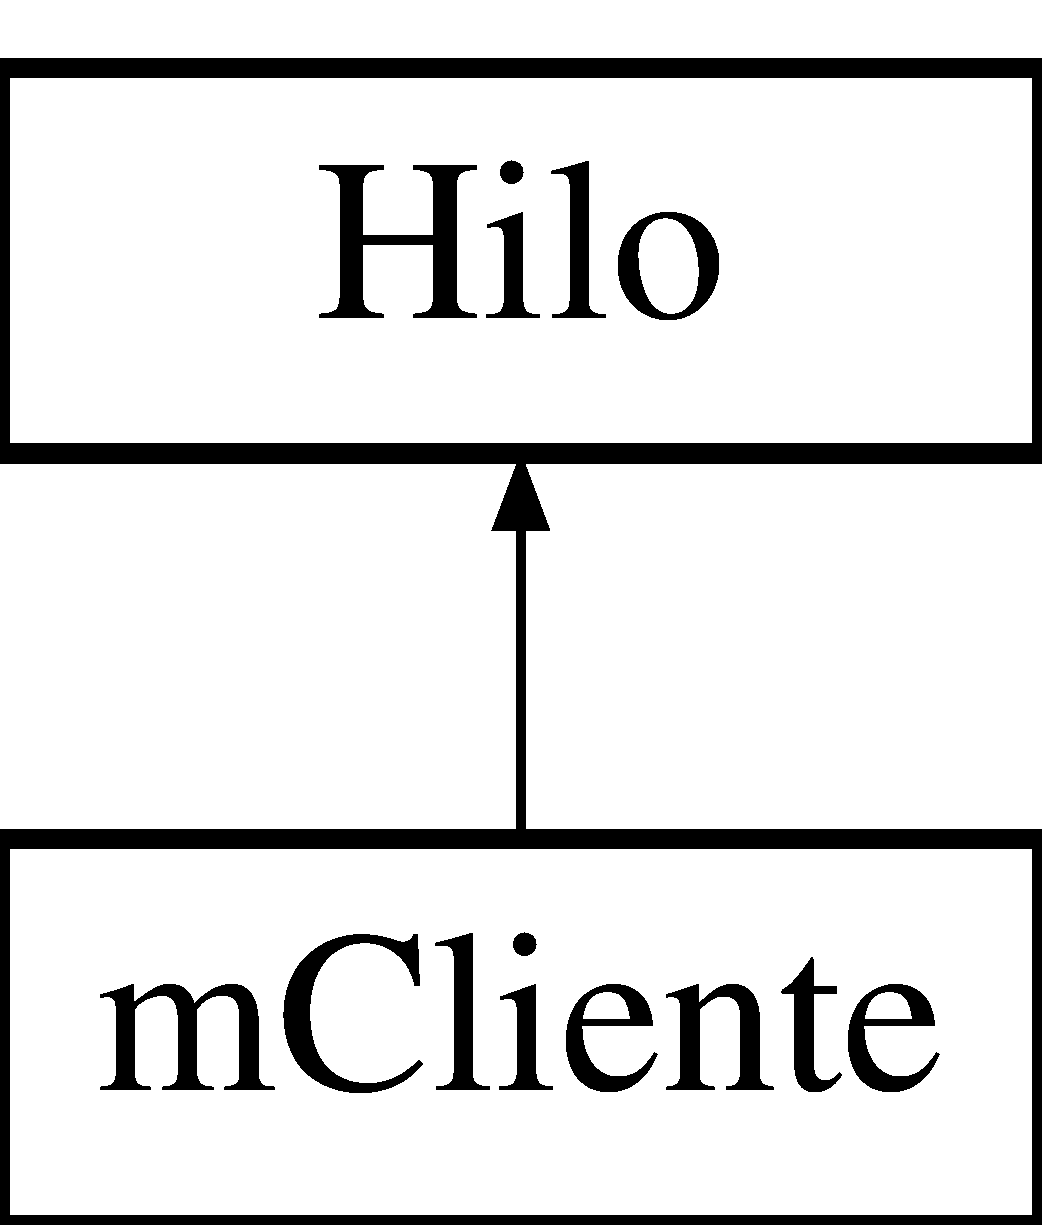
\includegraphics[height=2.000000cm]{classmCliente}
\end{center}
\end{figure}
\subsection*{\-Métodos públicos}
\begin{DoxyCompactItemize}
\item 
\hypertarget{classmCliente_acd61fb56f534263262f630f1899583b6}{{\bfseries m\-Cliente} (std\-::string h)}\label{classmCliente_acd61fb56f534263262f630f1899583b6}

\item 
\hypertarget{classmCliente_aaf850da977663d5596c3fb322b9cf164}{virtual void \hyperlink{classmCliente_aaf850da977663d5596c3fb322b9cf164}{correr} ()}\label{classmCliente_aaf850da977663d5596c3fb322b9cf164}

\begin{DoxyCompactList}\small\item\em \-Metodo virtual puro, que corre cuando se ejecuta el hilo. \end{DoxyCompactList}\end{DoxyCompactItemize}


\-La documentación para esta clase fue generada a partir del siguiente fichero\-:\begin{DoxyCompactItemize}
\item 
\-Pruebas/prueba\-Socket.\-h\end{DoxyCompactItemize}

\hypertarget{classMensaje}{\section{\-Referencia de la \-Clase \-Mensaje}
\label{classMensaje}\index{\-Mensaje@{\-Mensaje}}
}


{\ttfamily \#include $<$\-Mensaje.\-h$>$}

\-Diagrama de herencias de \-Mensaje\begin{figure}[H]
\begin{center}
\leavevmode
\includegraphics[height=2.000000cm]{classMensaje}
\end{center}
\end{figure}
\subsection*{\-Métodos públicos}
\begin{DoxyCompactItemize}
\item 
\hypertarget{classMensaje_a7b8b4ca08f400fef32eaffeec00f65b3}{\hyperlink{classMensaje_a7b8b4ca08f400fef32eaffeec00f65b3}{\-Mensaje} ()}\label{classMensaje_a7b8b4ca08f400fef32eaffeec00f65b3}

\begin{DoxyCompactList}\small\item\em \-Constructor sin \-Argumentos. \end{DoxyCompactList}\item 
virtual std\-::string \hyperlink{classMensaje_afd69cd129ca7ce1cf967a6f3690ad904}{serializar} () const =0
\begin{DoxyCompactList}\small\item\em \-Metodo que serializa todo el mensaje en un string. \end{DoxyCompactList}\item 
virtual void \hyperlink{classMensaje_a49422c2abf7fe32e887ee854cdf6cf25}{deserializar} (const std\-::string \&datos)=0
\begin{DoxyCompactList}\small\item\em \-Metodo que se deserialza a partir de un string. \end{DoxyCompactList}\end{DoxyCompactItemize}


\subsection{\-Descripción detallada}
\-Esta clase es abstracta y representa a la comunicacion habra entre un cliente con un servidor o un agente con un servidor. 

\subsection{\-Documentación de las funciones miembro}
\hypertarget{classMensaje_a49422c2abf7fe32e887ee854cdf6cf25}{\index{\-Mensaje@{\-Mensaje}!deserializar@{deserializar}}
\index{deserializar@{deserializar}!Mensaje@{\-Mensaje}}
\subsubsection[{deserializar}]{\setlength{\rightskip}{0pt plus 5cm}virtual void {\bf \-Mensaje\-::deserializar} (
\begin{DoxyParamCaption}
\item[{const std\-::string \&}]{datos}
\end{DoxyParamCaption}
)\hspace{0.3cm}{\ttfamily  \mbox{[}pure virtual\mbox{]}}}}\label{classMensaje_a49422c2abf7fe32e887ee854cdf6cf25}


\-Metodo que se deserialza a partir de un string. 


\begin{DoxyParams}{\-Parámetros}
{\em datos} & string que contiene el \hyperlink{classMensaje}{\-Mensaje} serializado. \\
\hline
\end{DoxyParams}


\-Implementado en \hyperlink{classConsulta_ac3edafd9d21258d9e2b2db753b6a0b61}{\-Consulta} y \hyperlink{classRespuesta_ae0481de83f0bdb1fd13d25885ce6e310}{\-Respuesta}.

\hypertarget{classMensaje_afd69cd129ca7ce1cf967a6f3690ad904}{\index{\-Mensaje@{\-Mensaje}!serializar@{serializar}}
\index{serializar@{serializar}!Mensaje@{\-Mensaje}}
\subsubsection[{serializar}]{\setlength{\rightskip}{0pt plus 5cm}virtual std\-::string {\bf \-Mensaje\-::serializar} (
\begin{DoxyParamCaption}
{}
\end{DoxyParamCaption}
) const\hspace{0.3cm}{\ttfamily  \mbox{[}pure virtual\mbox{]}}}}\label{classMensaje_afd69cd129ca7ce1cf967a6f3690ad904}


\-Metodo que serializa todo el mensaje en un string. 

\begin{DoxyReturn}{\-Devuelve}
string con el mensjae serializado. 
\end{DoxyReturn}


\-Implementado en \hyperlink{classConsulta_a0d3fd7d84c1a68b8cbe31a4118150269}{\-Consulta} y \hyperlink{classRespuesta_a3705c87e5738e9612410cb3567caf54c}{\-Respuesta}.



\-La documentación para esta clase fue generada a partir de los siguientes ficheros\-:\begin{DoxyCompactItemize}
\item 
comun/\-Mensaje.\-h\item 
comun/\-Mensaje.\-cpp\end{DoxyCompactItemize}

\hypertarget{classmServidor}{\section{\-Referencia de la \-Clase m\-Servidor}
\label{classmServidor}\index{m\-Servidor@{m\-Servidor}}
}
\-Diagrama de herencias de m\-Servidor\begin{figure}[H]
\begin{center}
\leavevmode
\includegraphics[height=2.000000cm]{classmServidor}
\end{center}
\end{figure}
\subsection*{\-Métodos públicos}
\begin{DoxyCompactItemize}
\item 
\hypertarget{classmServidor_a67e6c4e358e277a9638e304f4a5f412d}{virtual void \hyperlink{classmServidor_a67e6c4e358e277a9638e304f4a5f412d}{correr} ()}\label{classmServidor_a67e6c4e358e277a9638e304f4a5f412d}

\begin{DoxyCompactList}\small\item\em \-Metodo virtual puro, que corre cuando se ejecuta el hilo. \end{DoxyCompactList}\item 
\hypertarget{classmServidor_a67e6c4e358e277a9638e304f4a5f412d}{virtual void \hyperlink{classmServidor_a67e6c4e358e277a9638e304f4a5f412d}{correr} ()}\label{classmServidor_a67e6c4e358e277a9638e304f4a5f412d}

\begin{DoxyCompactList}\small\item\em \-Metodo virtual puro, que corre cuando se ejecuta el hilo. \end{DoxyCompactList}\end{DoxyCompactItemize}
\subsection*{\-Atributos públicos}
\begin{DoxyCompactItemize}
\item 
\hypertarget{classmServidor_a06cc1937fe9183585903babbf7d8580f}{\hyperlink{classSocket}{\-Socket} {\bfseries \-\_\-sck}}\label{classmServidor_a06cc1937fe9183585903babbf7d8580f}

\end{DoxyCompactItemize}


\-La documentación para esta clase fue generada a partir de los siguientes ficheros\-:\begin{DoxyCompactItemize}
\item 
\-Pruebas/\-Pruebas\-Agente.\-h\item 
\-Pruebas/prueba\-Socket.\-h\end{DoxyCompactItemize}

\hypertarget{classMutex}{\section{\-Referencia de la \-Clase \-Mutex}
\label{classMutex}\index{\-Mutex@{\-Mutex}}
}


{\ttfamily \#include $<$\-Mutex.\-h$>$}

\subsection*{\-Métodos públicos}
\begin{DoxyCompactItemize}
\item 
\hypertarget{classMutex_ad91be808bf0a60a16f10b897ec246d3a}{void {\bfseries lock} ()}\label{classMutex_ad91be808bf0a60a16f10b897ec246d3a}

\item 
\hypertarget{classMutex_aa1d3e908c776046ace50916fa6a3681f}{void {\bfseries signal} ()}\label{classMutex_aa1d3e908c776046ace50916fa6a3681f}

\item 
\hypertarget{classMutex_a70e3b0177eeb334bf8e7d42fa3edcc38}{void {\bfseries wait} ()}\label{classMutex_a70e3b0177eeb334bf8e7d42fa3edcc38}

\item 
\hypertarget{classMutex_a546a5b797ba29959357586aa2b3740a8}{void {\bfseries unlock} ()}\label{classMutex_a546a5b797ba29959357586aa2b3740a8}

\end{DoxyCompactItemize}
\subsection*{\-Amigas}
\begin{DoxyCompactItemize}
\item 
\hypertarget{classMutex_a5bf7608e05250fb524a1229bcf83ece3}{class {\bfseries \-Lock}}\label{classMutex_a5bf7608e05250fb524a1229bcf83ece3}

\end{DoxyCompactItemize}


\subsection{\-Descripción detallada}
\-Clase que enmascara el comportamiento de los pthread\-\_\-mutex de \-P\-O\-S\-I\-X. 

\-La documentación para esta clase fue generada a partir del siguiente fichero\-:\begin{DoxyCompactItemize}
\item 
comun/\-Mutex.\-h\end{DoxyCompactItemize}

\hypertarget{classOrganizacion}{\section{\-Referencia de la \-Clase \-Organizacion}
\label{classOrganizacion}\index{\-Organizacion@{\-Organizacion}}
}


{\ttfamily \#include $<$\-Organizacion.\-h$>$}

\subsection*{\-Métodos públicos estáticos}
\begin{DoxyCompactItemize}
\item 
static void \hyperlink{classOrganizacion_a78413f92453d9efa234a49dbb2afc4b9}{cargar\-Definiciones} (const std\-::string \&ruta\-Archivo=\-S\-T\-R\-\_\-\-N\-U\-L\-A)
\begin{DoxyCompactList}\small\item\em \-Carga los datos de la \-Informacion desde un archivo. \end{DoxyCompactList}\item 
static bool \hyperlink{classOrganizacion_a898670aaa00e73db489c2099fb7d5a14}{es\-Dimension} (const std\-::string \&\hyperlink{classOrganizacion_a07eb9a61b81f4d2d3aa4fc66ffdbbbfa}{nombre\-Campo})
\begin{DoxyCompactList}\small\item\em \-Indica si un campo de la \hyperlink{classOrganizacion}{\-Organizacion} es una \-Dimension. \end{DoxyCompactList}\item 
static bool \hyperlink{classOrganizacion_a27fad2197243739ae9ea80fe06382998}{es\-Hecho} (const std\-::string \&\hyperlink{classOrganizacion_a07eb9a61b81f4d2d3aa4fc66ffdbbbfa}{nombre\-Campo})
\begin{DoxyCompactList}\small\item\em \-Indica si un campo de la \hyperlink{classOrganizacion}{\-Organizacion} es un \hyperlink{classHecho}{\-Hecho}. \end{DoxyCompactList}\item 
static bool \hyperlink{classOrganizacion_aa08d3a99ce2020576dee9cbefa60ee2e}{es\-Dimension\-Especial} (const std\-::string \&\hyperlink{classOrganizacion_a07eb9a61b81f4d2d3aa4fc66ffdbbbfa}{nombre\-Campo})
\begin{DoxyCompactList}\small\item\em \-Indica si un campo de la \hyperlink{classOrganizacion}{\-Organizacion} es una \-Dimension \-Especial. \end{DoxyCompactList}\item 
static const std\-::string \& \hyperlink{classOrganizacion_a07eb9a61b81f4d2d3aa4fc66ffdbbbfa}{nombre\-Campo} (unsigned indice)
\begin{DoxyCompactList}\small\item\em \-Devuelve el nombre de un campo segun su indice en la \hyperlink{classOrganizacion}{\-Organizacion}. \-Si no existe un nombre para el indice argumento, se retorna un string nulo. \end{DoxyCompactList}\item 
static const std\-::string \& \hyperlink{classOrganizacion_a97c881f33d02fb1301ff5edfc3c5c39f}{nombre\-Campo\-Simple} (unsigned indice)
\begin{DoxyCompactList}\small\item\em \-Devuelve el nombre de un campo simple segun su indice en la \hyperlink{classOrganizacion}{\-Organizacion}. \-Si no existe un nombre para el indice argumento, se retorna un string nulo. \end{DoxyCompactList}\item 
static const std\-::string \& \hyperlink{classOrganizacion_afdcbc32f5a48c21d8d814f2289462a68}{nombre\-Dimension} (unsigned indice)
\begin{DoxyCompactList}\small\item\em \-Devuelve el nombre de una \-Dimension segun su indice en la \hyperlink{classOrganizacion}{\-Organizacion}. \-Si no existe un nombre para el indice argumento, se retorna un string nulo. \end{DoxyCompactList}\item 
static const std\-::string \& \hyperlink{classOrganizacion_a9f9ba53d668e5a6e1056d10bb2494cd8}{nombre\-Dimension\-Simple} (unsigned indice)
\begin{DoxyCompactList}\small\item\em \-Devuelve el nombre de una \-Dimension segun su indice en la \hyperlink{classOrganizacion}{\-Organizacion}. \-Si no existe un nombre para el indice argumento, se retorna un string nulo. \end{DoxyCompactList}\item 
static const std\-::string \& \hyperlink{classOrganizacion_aa5ccaedf53bdce391f7e0dd8f23a0892}{nombre\-Hecho} (unsigned indice)
\begin{DoxyCompactList}\small\item\em \-Devuelve el nombre de un \hyperlink{classHecho}{\-Hecho} segun su indice en la \hyperlink{classOrganizacion}{\-Organizacion}. \-Si no existe un nombre para el indice argumento, se retorna un string nulo. \end{DoxyCompactList}\item 
static unsigned \hyperlink{classOrganizacion_ab5305f1db341422c2993403f7341ddbd}{indice\-De\-Campo} (const std\-::string \&campo)
\begin{DoxyCompactList}\small\item\em \-Indica cual es el indice de un \-Campo segun su \-Nombre. \end{DoxyCompactList}\item 
static unsigned \hyperlink{classOrganizacion_a45acfeb9509942abf6ed92e71172956b}{indice\-De\-Campo\-Simple} (const std\-::string \&campo)
\begin{DoxyCompactList}\small\item\em \-Indica cual es el indice de un \-Campo \-Simple segun su \-Nombre. \end{DoxyCompactList}\item 
static unsigned \hyperlink{classOrganizacion_afb5a828d0c88b8ee98dfff1312ab8b5f}{cantidad\-Hechos} ()
\begin{DoxyCompactList}\small\item\em \-Indica la cantidad de \-Hechos en la \-Organización. \end{DoxyCompactList}\item 
static unsigned \hyperlink{classOrganizacion_ac42240de149c9d37c7c7c643a088c674}{cantidad\-Dimensiones\-Total} ()
\begin{DoxyCompactList}\small\item\em \-Indica la cantidad de \-Dimensiones que posee la \-Organización. \end{DoxyCompactList}\item 
static unsigned \hyperlink{classOrganizacion_a1de553b411941d89bec3327f94e9f323}{cantidad\-Dimensiones\-Simples} ()
\begin{DoxyCompactList}\small\item\em \-Indica la cantidad de \-Dimensiones \-Simples que posee la \-Organización. \end{DoxyCompactList}\item 
static unsigned \hyperlink{classOrganizacion_a160c3a4f7cc86807c244f6904a3c1adf}{cantidad\-Campos} ()
\begin{DoxyCompactList}\small\item\em \-Indica la cantidad de \-Campos que posee la \-Organización. \end{DoxyCompactList}\item 
static unsigned \hyperlink{classOrganizacion_a8b6bf6303d8ccfa9b36d1b1389f0bef5}{cantidad\-Campos\-Simples} ()
\begin{DoxyCompactList}\small\item\em \-Indica la cantidad de \-Campos \-Simples que posee la \hyperlink{classOrganizacion}{\-Organizacion}. \end{DoxyCompactList}\end{DoxyCompactItemize}


\subsection{\-Descripción detallada}
\-Esta clase estatica encargada de cargar, guardar el modole del \-Archivo, pudiendo consultar sobre sus dimensiones, hechos, y cantidades que hay de estos, es decir, se encarga de resolver toda cuestion que implicase al modelo. \-La clasificacion de la \-Organizacino es la siguiente, las \-Dimensiones estan conformadas por \-Dimensiones simples y \-Dimensiones \-Especiales,en los \-Hechos no existe esta distincion, siendo los \-Campos comformados por \-Dimensiones y \-Hechos,un ejemplo de clasificacion seria que los \-Campos simples estan conformados por \-Dimensiones \-Simples y \-Hechos. \-El funcionamiento de esta clase es solo de consulta para cuestiones que involucren al modelo de datos. 

\subsection{\-Documentación de las funciones miembro}
\hypertarget{classOrganizacion_a160c3a4f7cc86807c244f6904a3c1adf}{\index{\-Organizacion@{\-Organizacion}!cantidad\-Campos@{cantidad\-Campos}}
\index{cantidad\-Campos@{cantidad\-Campos}!Organizacion@{\-Organizacion}}
\subsubsection[{cantidad\-Campos}]{\setlength{\rightskip}{0pt plus 5cm}unsigned {\bf \-Organizacion\-::cantidad\-Campos} (
\begin{DoxyParamCaption}
{}
\end{DoxyParamCaption}
)\hspace{0.3cm}{\ttfamily  \mbox{[}static\mbox{]}}}}\label{classOrganizacion_a160c3a4f7cc86807c244f6904a3c1adf}


\-Indica la cantidad de \-Campos que posee la \-Organización. 

\begin{DoxyReturn}{\-Devuelve}
cantidad de \-Campos. 
\end{DoxyReturn}
\hypertarget{classOrganizacion_a8b6bf6303d8ccfa9b36d1b1389f0bef5}{\index{\-Organizacion@{\-Organizacion}!cantidad\-Campos\-Simples@{cantidad\-Campos\-Simples}}
\index{cantidad\-Campos\-Simples@{cantidad\-Campos\-Simples}!Organizacion@{\-Organizacion}}
\subsubsection[{cantidad\-Campos\-Simples}]{\setlength{\rightskip}{0pt plus 5cm}unsigned {\bf \-Organizacion\-::cantidad\-Campos\-Simples} (
\begin{DoxyParamCaption}
{}
\end{DoxyParamCaption}
)\hspace{0.3cm}{\ttfamily  \mbox{[}static\mbox{]}}}}\label{classOrganizacion_a8b6bf6303d8ccfa9b36d1b1389f0bef5}


\-Indica la cantidad de \-Campos \-Simples que posee la \hyperlink{classOrganizacion}{\-Organizacion}. 

\begin{DoxyReturn}{\-Devuelve}
cantidad de \-Campos \-Simples. 
\end{DoxyReturn}
\hypertarget{classOrganizacion_a1de553b411941d89bec3327f94e9f323}{\index{\-Organizacion@{\-Organizacion}!cantidad\-Dimensiones\-Simples@{cantidad\-Dimensiones\-Simples}}
\index{cantidad\-Dimensiones\-Simples@{cantidad\-Dimensiones\-Simples}!Organizacion@{\-Organizacion}}
\subsubsection[{cantidad\-Dimensiones\-Simples}]{\setlength{\rightskip}{0pt plus 5cm}unsigned {\bf \-Organizacion\-::cantidad\-Dimensiones\-Simples} (
\begin{DoxyParamCaption}
{}
\end{DoxyParamCaption}
)\hspace{0.3cm}{\ttfamily  \mbox{[}static\mbox{]}}}}\label{classOrganizacion_a1de553b411941d89bec3327f94e9f323}


\-Indica la cantidad de \-Dimensiones \-Simples que posee la \-Organización. 

\begin{DoxyReturn}{\-Devuelve}
cantidad de \-Dimensiones \-Simples. 
\end{DoxyReturn}
\hypertarget{classOrganizacion_ac42240de149c9d37c7c7c643a088c674}{\index{\-Organizacion@{\-Organizacion}!cantidad\-Dimensiones\-Total@{cantidad\-Dimensiones\-Total}}
\index{cantidad\-Dimensiones\-Total@{cantidad\-Dimensiones\-Total}!Organizacion@{\-Organizacion}}
\subsubsection[{cantidad\-Dimensiones\-Total}]{\setlength{\rightskip}{0pt plus 5cm}unsigned {\bf \-Organizacion\-::cantidad\-Dimensiones\-Total} (
\begin{DoxyParamCaption}
{}
\end{DoxyParamCaption}
)\hspace{0.3cm}{\ttfamily  \mbox{[}static\mbox{]}}}}\label{classOrganizacion_ac42240de149c9d37c7c7c643a088c674}


\-Indica la cantidad de \-Dimensiones que posee la \-Organización. 

\begin{DoxyReturn}{\-Devuelve}
cantidad de \-Dimensiones. 
\end{DoxyReturn}
\hypertarget{classOrganizacion_afb5a828d0c88b8ee98dfff1312ab8b5f}{\index{\-Organizacion@{\-Organizacion}!cantidad\-Hechos@{cantidad\-Hechos}}
\index{cantidad\-Hechos@{cantidad\-Hechos}!Organizacion@{\-Organizacion}}
\subsubsection[{cantidad\-Hechos}]{\setlength{\rightskip}{0pt plus 5cm}unsigned {\bf \-Organizacion\-::cantidad\-Hechos} (
\begin{DoxyParamCaption}
{}
\end{DoxyParamCaption}
)\hspace{0.3cm}{\ttfamily  \mbox{[}static\mbox{]}}}}\label{classOrganizacion_afb5a828d0c88b8ee98dfff1312ab8b5f}


\-Indica la cantidad de \-Hechos en la \-Organización. 

\begin{DoxyReturn}{\-Devuelve}
cantidad de \-Hechos. 
\end{DoxyReturn}
\hypertarget{classOrganizacion_a78413f92453d9efa234a49dbb2afc4b9}{\index{\-Organizacion@{\-Organizacion}!cargar\-Definiciones@{cargar\-Definiciones}}
\index{cargar\-Definiciones@{cargar\-Definiciones}!Organizacion@{\-Organizacion}}
\subsubsection[{cargar\-Definiciones}]{\setlength{\rightskip}{0pt plus 5cm}void {\bf \-Organizacion\-::cargar\-Definiciones} (
\begin{DoxyParamCaption}
\item[{const std\-::string \&}]{ruta\-Archivo = {\ttfamily \-S\-T\-R\-\_\-\-N\-U\-L\-A}}
\end{DoxyParamCaption}
)\hspace{0.3cm}{\ttfamily  \mbox{[}static\mbox{]}}}}\label{classOrganizacion_a78413f92453d9efa234a49dbb2afc4b9}


\-Carga los datos de la \-Informacion desde un archivo. 


\begin{DoxyParams}{\-Parámetros}
{\em ruta\-Archivo} & string que contiene la ruta del archivo. \-Si no se especifica la ruta se utilizara la ruta por defecto. \\
\hline
\end{DoxyParams}
\hypertarget{classOrganizacion_a898670aaa00e73db489c2099fb7d5a14}{\index{\-Organizacion@{\-Organizacion}!es\-Dimension@{es\-Dimension}}
\index{es\-Dimension@{es\-Dimension}!Organizacion@{\-Organizacion}}
\subsubsection[{es\-Dimension}]{\setlength{\rightskip}{0pt plus 5cm}bool {\bf \-Organizacion\-::es\-Dimension} (
\begin{DoxyParamCaption}
\item[{const std\-::string \&}]{nombre\-Campo}
\end{DoxyParamCaption}
)\hspace{0.3cm}{\ttfamily  \mbox{[}static\mbox{]}}}}\label{classOrganizacion_a898670aaa00e73db489c2099fb7d5a14}


\-Indica si un campo de la \hyperlink{classOrganizacion}{\-Organizacion} es una \-Dimension. 


\begin{DoxyParams}{\-Parámetros}
{\em nombre\-Campo} & campo a analizar. \\
\hline
\end{DoxyParams}
\begin{DoxyReturn}{\-Devuelve}
booleano que indica el resultado. 
\end{DoxyReturn}
\hypertarget{classOrganizacion_aa08d3a99ce2020576dee9cbefa60ee2e}{\index{\-Organizacion@{\-Organizacion}!es\-Dimension\-Especial@{es\-Dimension\-Especial}}
\index{es\-Dimension\-Especial@{es\-Dimension\-Especial}!Organizacion@{\-Organizacion}}
\subsubsection[{es\-Dimension\-Especial}]{\setlength{\rightskip}{0pt plus 5cm}bool {\bf \-Organizacion\-::es\-Dimension\-Especial} (
\begin{DoxyParamCaption}
\item[{const std\-::string \&}]{nombre\-Campo}
\end{DoxyParamCaption}
)\hspace{0.3cm}{\ttfamily  \mbox{[}static\mbox{]}}}}\label{classOrganizacion_aa08d3a99ce2020576dee9cbefa60ee2e}


\-Indica si un campo de la \hyperlink{classOrganizacion}{\-Organizacion} es una \-Dimension \-Especial. 


\begin{DoxyParams}{\-Parámetros}
{\em nombre\-Campo} & campo a analizar. \\
\hline
\end{DoxyParams}
\begin{DoxyReturn}{\-Devuelve}
booleano que indica el resultado. 
\end{DoxyReturn}
\hypertarget{classOrganizacion_a27fad2197243739ae9ea80fe06382998}{\index{\-Organizacion@{\-Organizacion}!es\-Hecho@{es\-Hecho}}
\index{es\-Hecho@{es\-Hecho}!Organizacion@{\-Organizacion}}
\subsubsection[{es\-Hecho}]{\setlength{\rightskip}{0pt plus 5cm}bool {\bf \-Organizacion\-::es\-Hecho} (
\begin{DoxyParamCaption}
\item[{const std\-::string \&}]{nombre\-Campo}
\end{DoxyParamCaption}
)\hspace{0.3cm}{\ttfamily  \mbox{[}static\mbox{]}}}}\label{classOrganizacion_a27fad2197243739ae9ea80fe06382998}


\-Indica si un campo de la \hyperlink{classOrganizacion}{\-Organizacion} es un \hyperlink{classHecho}{\-Hecho}. 


\begin{DoxyParams}{\-Parámetros}
{\em nombre\-Campo} & campo a analizar. \\
\hline
\end{DoxyParams}
\begin{DoxyReturn}{\-Devuelve}
booleano que indica el resultado. 
\end{DoxyReturn}
\hypertarget{classOrganizacion_ab5305f1db341422c2993403f7341ddbd}{\index{\-Organizacion@{\-Organizacion}!indice\-De\-Campo@{indice\-De\-Campo}}
\index{indice\-De\-Campo@{indice\-De\-Campo}!Organizacion@{\-Organizacion}}
\subsubsection[{indice\-De\-Campo}]{\setlength{\rightskip}{0pt plus 5cm}unsigned {\bf \-Organizacion\-::indice\-De\-Campo} (
\begin{DoxyParamCaption}
\item[{const std\-::string \&}]{campo}
\end{DoxyParamCaption}
)\hspace{0.3cm}{\ttfamily  \mbox{[}static\mbox{]}}}}\label{classOrganizacion_ab5305f1db341422c2993403f7341ddbd}


\-Indica cual es el indice de un \-Campo segun su \-Nombre. 


\begin{DoxyParams}{\-Parámetros}
{\em campo} & nombre del \-Campo recuperar su indice. \\
\hline
\end{DoxyParams}
\begin{DoxyReturn}{\-Devuelve}
indice del campo. 
\end{DoxyReturn}
\hypertarget{classOrganizacion_a45acfeb9509942abf6ed92e71172956b}{\index{\-Organizacion@{\-Organizacion}!indice\-De\-Campo\-Simple@{indice\-De\-Campo\-Simple}}
\index{indice\-De\-Campo\-Simple@{indice\-De\-Campo\-Simple}!Organizacion@{\-Organizacion}}
\subsubsection[{indice\-De\-Campo\-Simple}]{\setlength{\rightskip}{0pt plus 5cm}unsigned {\bf \-Organizacion\-::indice\-De\-Campo\-Simple} (
\begin{DoxyParamCaption}
\item[{const std\-::string \&}]{campo}
\end{DoxyParamCaption}
)\hspace{0.3cm}{\ttfamily  \mbox{[}static\mbox{]}}}}\label{classOrganizacion_a45acfeb9509942abf6ed92e71172956b}


\-Indica cual es el indice de un \-Campo \-Simple segun su \-Nombre. 


\begin{DoxyParams}{\-Parámetros}
{\em campo} & nombre del \-Campo \-Simple recuperar su indice. \\
\hline
\end{DoxyParams}
\begin{DoxyReturn}{\-Devuelve}
indice del \-Campo \-Simple. 
\end{DoxyReturn}
\hypertarget{classOrganizacion_a07eb9a61b81f4d2d3aa4fc66ffdbbbfa}{\index{\-Organizacion@{\-Organizacion}!nombre\-Campo@{nombre\-Campo}}
\index{nombre\-Campo@{nombre\-Campo}!Organizacion@{\-Organizacion}}
\subsubsection[{nombre\-Campo}]{\setlength{\rightskip}{0pt plus 5cm}const std\-::string \& {\bf \-Organizacion\-::nombre\-Campo} (
\begin{DoxyParamCaption}
\item[{unsigned}]{indice}
\end{DoxyParamCaption}
)\hspace{0.3cm}{\ttfamily  \mbox{[}static\mbox{]}}}}\label{classOrganizacion_a07eb9a61b81f4d2d3aa4fc66ffdbbbfa}


\-Devuelve el nombre de un campo segun su indice en la \hyperlink{classOrganizacion}{\-Organizacion}. \-Si no existe un nombre para el indice argumento, se retorna un string nulo. 


\begin{DoxyParams}{\-Parámetros}
{\em indice} & es indice del \-Campo a recuperar. \\
\hline
\end{DoxyParams}
\begin{DoxyReturn}{\-Devuelve}
string que contiene el nombre del campo. 
\end{DoxyReturn}
\hypertarget{classOrganizacion_a97c881f33d02fb1301ff5edfc3c5c39f}{\index{\-Organizacion@{\-Organizacion}!nombre\-Campo\-Simple@{nombre\-Campo\-Simple}}
\index{nombre\-Campo\-Simple@{nombre\-Campo\-Simple}!Organizacion@{\-Organizacion}}
\subsubsection[{nombre\-Campo\-Simple}]{\setlength{\rightskip}{0pt plus 5cm}const std\-::string \& {\bf \-Organizacion\-::nombre\-Campo\-Simple} (
\begin{DoxyParamCaption}
\item[{unsigned}]{indice}
\end{DoxyParamCaption}
)\hspace{0.3cm}{\ttfamily  \mbox{[}static\mbox{]}}}}\label{classOrganizacion_a97c881f33d02fb1301ff5edfc3c5c39f}


\-Devuelve el nombre de un campo simple segun su indice en la \hyperlink{classOrganizacion}{\-Organizacion}. \-Si no existe un nombre para el indice argumento, se retorna un string nulo. 


\begin{DoxyParams}{\-Parámetros}
{\em indice} & es indice del \-Campo \-Simple a recuperar. \\
\hline
\end{DoxyParams}
\begin{DoxyReturn}{\-Devuelve}
string que contiene el nombre del \-Campo \-Simple recuperado. 
\end{DoxyReturn}
\hypertarget{classOrganizacion_afdcbc32f5a48c21d8d814f2289462a68}{\index{\-Organizacion@{\-Organizacion}!nombre\-Dimension@{nombre\-Dimension}}
\index{nombre\-Dimension@{nombre\-Dimension}!Organizacion@{\-Organizacion}}
\subsubsection[{nombre\-Dimension}]{\setlength{\rightskip}{0pt plus 5cm}const std\-::string \& {\bf \-Organizacion\-::nombre\-Dimension} (
\begin{DoxyParamCaption}
\item[{unsigned}]{indice}
\end{DoxyParamCaption}
)\hspace{0.3cm}{\ttfamily  \mbox{[}static\mbox{]}}}}\label{classOrganizacion_afdcbc32f5a48c21d8d814f2289462a68}


\-Devuelve el nombre de una \-Dimension segun su indice en la \hyperlink{classOrganizacion}{\-Organizacion}. \-Si no existe un nombre para el indice argumento, se retorna un string nulo. 


\begin{DoxyParams}{\-Parámetros}
{\em indice} & es indice de la \-Dimension a recuperar. \\
\hline
\end{DoxyParams}
\begin{DoxyReturn}{\-Devuelve}
string que contiene la \-Dimension recuperada. 
\end{DoxyReturn}
\hypertarget{classOrganizacion_a9f9ba53d668e5a6e1056d10bb2494cd8}{\index{\-Organizacion@{\-Organizacion}!nombre\-Dimension\-Simple@{nombre\-Dimension\-Simple}}
\index{nombre\-Dimension\-Simple@{nombre\-Dimension\-Simple}!Organizacion@{\-Organizacion}}
\subsubsection[{nombre\-Dimension\-Simple}]{\setlength{\rightskip}{0pt plus 5cm}const std\-::string \& {\bf \-Organizacion\-::nombre\-Dimension\-Simple} (
\begin{DoxyParamCaption}
\item[{unsigned}]{indice}
\end{DoxyParamCaption}
)\hspace{0.3cm}{\ttfamily  \mbox{[}static\mbox{]}}}}\label{classOrganizacion_a9f9ba53d668e5a6e1056d10bb2494cd8}


\-Devuelve el nombre de una \-Dimension segun su indice en la \hyperlink{classOrganizacion}{\-Organizacion}. \-Si no existe un nombre para el indice argumento, se retorna un string nulo. 


\begin{DoxyParams}{\-Parámetros}
{\em indice} & es el indice de la \-Dimension \-Simple a recuperar. \\
\hline
\end{DoxyParams}
\begin{DoxyReturn}{\-Devuelve}
string que contiene la \-Dimesion \-Simple recuperada. 
\end{DoxyReturn}
\hypertarget{classOrganizacion_aa5ccaedf53bdce391f7e0dd8f23a0892}{\index{\-Organizacion@{\-Organizacion}!nombre\-Hecho@{nombre\-Hecho}}
\index{nombre\-Hecho@{nombre\-Hecho}!Organizacion@{\-Organizacion}}
\subsubsection[{nombre\-Hecho}]{\setlength{\rightskip}{0pt plus 5cm}const std\-::string \& {\bf \-Organizacion\-::nombre\-Hecho} (
\begin{DoxyParamCaption}
\item[{unsigned}]{indice}
\end{DoxyParamCaption}
)\hspace{0.3cm}{\ttfamily  \mbox{[}static\mbox{]}}}}\label{classOrganizacion_aa5ccaedf53bdce391f7e0dd8f23a0892}


\-Devuelve el nombre de un \hyperlink{classHecho}{\-Hecho} segun su indice en la \hyperlink{classOrganizacion}{\-Organizacion}. \-Si no existe un nombre para el indice argumento, se retorna un string nulo. 


\begin{DoxyParams}{\-Parámetros}
{\em indice} & es l indice del \hyperlink{classHecho}{\-Hecho} a recuperar \\
\hline
\end{DoxyParams}
\begin{DoxyReturn}{\-Devuelve}
string que contiene el \hyperlink{classHecho}{\-Hecho} recuperado. 
\end{DoxyReturn}


\-La documentación para esta clase fue generada a partir de los siguientes ficheros\-:\begin{DoxyCompactItemize}
\item 
comun/\-Organizacion.\-h\item 
comun/\-Organizacion.\-cpp\end{DoxyCompactItemize}

\hypertarget{classPanel}{\section{\-Referencia de la \-Clase \-Panel}
\label{classPanel}\index{\-Panel@{\-Panel}}
}


{\ttfamily \#include $<$\-Panel.\-h$>$}

\subsection*{\-Métodos públicos}
\begin{DoxyCompactItemize}
\item 
\hyperlink{classPanel_a472972c00119ab21bea8ab60327c54fd}{\-Panel} (const \-Glib\-::ustring \&label)
\item 
\hyperlink{classPanel_a93893b8e3923462b52e06e0003d11448}{$\sim$\-Panel} ()
\item 
\hypertarget{classPanel_a22125b7d4dc9e8c4fe59f432bf8bae2e}{void {\bfseries set\-Contenido} (\hyperlink{classGrafico}{\-Grafico} \&g)}\label{classPanel_a22125b7d4dc9e8c4fe59f432bf8bae2e}

\item 
\hypertarget{classPanel_a01bf0212b192c969fc78ff1594b2ea85}{void {\bfseries set\-Contenido} (\hyperlink{classTabla}{\-Tabla} \&t)}\label{classPanel_a01bf0212b192c969fc78ff1594b2ea85}

\item 
\hypertarget{classPanel_a0d401a477ecdaecc68bb603b2a805955}{\hyperlink{classConsultante}{\-Consultante} $\ast$ {\bfseries get\-Consultante} ()}\label{classPanel_a0d401a477ecdaecc68bb603b2a805955}

\end{DoxyCompactItemize}


\subsection{\-Descripción detallada}
\-Clase que representa visualmente una consulta configurada. \-Además de contener un consultante (sea gráfico o tabla), tiene un conjunto de filtradores, y el título con que fue guardado. 

\subsection{\-Documentación del constructor y destructor}
\hypertarget{classPanel_a472972c00119ab21bea8ab60327c54fd}{\index{\-Panel@{\-Panel}!\-Panel@{\-Panel}}
\index{\-Panel@{\-Panel}!Panel@{\-Panel}}
\subsubsection[{\-Panel}]{\setlength{\rightskip}{0pt plus 5cm}{\bf \-Panel\-::\-Panel} (
\begin{DoxyParamCaption}
\item[{const \-Glib\-::ustring \&}]{label}
\end{DoxyParamCaption}
)}}\label{classPanel_a472972c00119ab21bea8ab60327c54fd}
\-Constructor. 
\begin{DoxyParams}{\-Parámetros}
{\em label} & título del panel \\
\hline
\end{DoxyParams}
\hypertarget{classPanel_a93893b8e3923462b52e06e0003d11448}{\index{\-Panel@{\-Panel}!$\sim$\-Panel@{$\sim$\-Panel}}
\index{$\sim$\-Panel@{$\sim$\-Panel}!Panel@{\-Panel}}
\subsubsection[{$\sim$\-Panel}]{\setlength{\rightskip}{0pt plus 5cm}{\bf \-Panel\-::$\sim$\-Panel} (
\begin{DoxyParamCaption}
{}
\end{DoxyParamCaption}
)}}\label{classPanel_a93893b8e3923462b52e06e0003d11448}
\-Destructor. 

\-La documentación para esta clase fue generada a partir de los siguientes ficheros\-:\begin{DoxyCompactItemize}
\item 
cliente/\-Vista/\-Panel.\-h\item 
cliente/\-Vista/\-Panel.\-cpp\end{DoxyCompactItemize}

\hypertarget{classPanelConfigModelo}{\section{\-Referencia de la \-Clase \-Panel\-Config\-Modelo}
\label{classPanelConfigModelo}\index{\-Panel\-Config\-Modelo@{\-Panel\-Config\-Modelo}}
}


{\ttfamily \#include $<$\-Panel\-Config\-Modelo.\-h$>$}

\-Diagrama de herencias de \-Panel\-Config\-Modelo\begin{figure}[H]
\begin{center}
\leavevmode
\includegraphics[height=3.000000cm]{classPanelConfigModelo}
\end{center}
\end{figure}
\subsection*{\-Métodos públicos}
\begin{DoxyCompactItemize}
\item 
\hyperlink{classPanelConfigModelo_a9a807a8f717b7e592143293df72268d3}{\-Panel\-Config\-Modelo} ()
\item 
\hyperlink{classPanelConfigModelo_a9939a132ddf4630dac47597f42ab144f}{$\sim$\-Panel\-Config\-Modelo} ()
\item 
\hypertarget{classPanelConfigModelo_ab7cbf97595cd65d7ab222723afe616d6}{void {\bfseries set\-Label\-Posicion} (\-Gtk\-::\-Label $\ast$p\-Label)}\label{classPanelConfigModelo_ab7cbf97595cd65d7ab222723afe616d6}

\item 
\hypertarget{classPanelConfigModelo_a89cacb1393bc8a6c22a78b77385fed56}{void {\bfseries set\-Spinbuttons\-Posicion} (\-Gtk\-::\-Spin\-Button $\ast$p\-Spinbuttondesde\-Fila, \-Gtk\-::\-Spin\-Button $\ast$p\-Spinbuttonhasta\-Fila, \-Gtk\-::\-Spin\-Button $\ast$p\-Spinbutton\-Desde\-Col, \-Gtk\-::\-Spin\-Button $\ast$p\-Spinbutton\-Hasta\-Col)}\label{classPanelConfigModelo_a89cacb1393bc8a6c22a78b77385fed56}

\item 
\hypertarget{classPanelConfigModelo_a8b005131e24623de4219ed9c42958b31}{void {\bfseries set\-Posicion\-Nueva\-Como\-Valida} (bool valida=true)}\label{classPanelConfigModelo_a8b005131e24623de4219ed9c42958b31}

\item 
\hypertarget{classPanelConfigModelo_a0c84ddef18f7f04988882158554e0547}{void {\bfseries set\-Combobox\-Tipo\-Grafico} (\-Gtk\-::\-Combo\-Box\-Text $\ast$p\-Combo)}\label{classPanelConfigModelo_a0c84ddef18f7f04988882158554e0547}

\item 
\hypertarget{classPanelConfigModelo_afd23979a56f30e04f26dba6afc3914f6}{void {\bfseries set\-Expanders\-Pivote} (\-Gtk\-::\-Expander $\ast$p\-X\-Pivote, \-Gtk\-::\-Expander $\ast$p\-Y\-Pivote)}\label{classPanelConfigModelo_afd23979a56f30e04f26dba6afc3914f6}

\item 
\hypertarget{classPanelConfigModelo_afeab7c9180fde4e4735f25c248756fa4}{void {\bfseries set\-Filtros\-Handlers} (const filtradores\-Handlers \&handlers)}\label{classPanelConfigModelo_afeab7c9180fde4e4735f25c248756fa4}

\item 
\hypertarget{classPanelConfigModelo_acee78ee197e593807bba82616e2d517a}{void {\bfseries set\-Inputs\-Handlers} (const filtradores\-Handlers \&handlers)}\label{classPanelConfigModelo_acee78ee197e593807bba82616e2d517a}

\item 
\hypertarget{classPanelConfigModelo_a074528361c531696e3f4e4dacd45b196}{void {\bfseries set\-Pivote\-Xs\-Handlers} (const filtradores\-Handlers \&handlers)}\label{classPanelConfigModelo_a074528361c531696e3f4e4dacd45b196}

\item 
\hypertarget{classPanelConfigModelo_a7d4eb8fc4bfd451123ae9a7f1505d377}{void {\bfseries set\-Pivote\-Ys\-Handlers} (const filtradores\-Handlers \&handlers)}\label{classPanelConfigModelo_a7d4eb8fc4bfd451123ae9a7f1505d377}

\item 
\hypertarget{classPanelConfigModelo_a51720317d2e5bdccb493e0354b28e174}{void {\bfseries set\-Resultados\-Handlers} (const filtradores\-Handlers \&handlers)}\label{classPanelConfigModelo_a51720317d2e5bdccb493e0354b28e174}

\item 
\hypertarget{classPanelConfigModelo_a39162a3267fa44354b6fdda51079cd54}{void {\bfseries get\-Posicion} (int \&desde\-Fila, int \&hasta\-Fila, int \&desde\-Col, int \&hasta\-Col)}\label{classPanelConfigModelo_a39162a3267fa44354b6fdda51079cd54}

\item 
\hypertarget{classPanelConfigModelo_ac31c5c8a464ffb215bad14b73e6f6f99}{sigc\-::signal$<$ void, \*
\hyperlink{classPanelConfigModelo}{\-Panel\-Config\-Modelo} $\ast$, int, int, \*
int, int $>$ {\bfseries signal\-\_\-posicion\-\_\-changed} ()}\label{classPanelConfigModelo_ac31c5c8a464ffb215bad14b73e6f6f99}

\item 
\hypertarget{classPanelConfigModelo_afba32582089d3bb5ac121689b36efb64}{\hyperlink{classPanel}{\-Panel} $\ast$ {\bfseries concretar\-Config} (\hyperlink{classFiltradoresPanel}{\-Filtradores\-Panel} $\ast$filt\-Panel)}\label{classPanelConfigModelo_afba32582089d3bb5ac121689b36efb64}

\item 
\hypertarget{classPanelConfigModelo_af0b826a63401e1c1e47ef2e7f2d6162a}{virtual \hyperlink{classTiXmlElement}{\-Nodo\-Xml} {\bfseries serializar} ()}\label{classPanelConfigModelo_af0b826a63401e1c1e47ef2e7f2d6162a}

\item 
\hypertarget{classPanelConfigModelo_a21dc033acbca37640841f1d76beb3abb}{virtual void {\bfseries deserializar} (const \hyperlink{classTiXmlElement}{\-Nodo\-Xml} \&nodo)}\label{classPanelConfigModelo_a21dc033acbca37640841f1d76beb3abb}

\end{DoxyCompactItemize}


\subsection{\-Descripción detallada}
\-Clase concreta que modela la configuración de un panel.

\-Un método importante que posee es \-Panel$\ast$ concretar\-Config(), dado que mediante este se generan los entes mismos de la aplicación, capaces de mostrar los filtradores aplicados, hacer consultas y representar gráficamente respuestas. 

\subsection{\-Documentación del constructor y destructor}
\hypertarget{classPanelConfigModelo_a9a807a8f717b7e592143293df72268d3}{\index{\-Panel\-Config\-Modelo@{\-Panel\-Config\-Modelo}!\-Panel\-Config\-Modelo@{\-Panel\-Config\-Modelo}}
\index{\-Panel\-Config\-Modelo@{\-Panel\-Config\-Modelo}!PanelConfigModelo@{\-Panel\-Config\-Modelo}}
\subsubsection[{\-Panel\-Config\-Modelo}]{\setlength{\rightskip}{0pt plus 5cm}{\bf \-Panel\-Config\-Modelo\-::\-Panel\-Config\-Modelo} (
\begin{DoxyParamCaption}
{}
\end{DoxyParamCaption}
)}}\label{classPanelConfigModelo_a9a807a8f717b7e592143293df72268d3}
\-Constructor. \hypertarget{classPanelConfigModelo_a9939a132ddf4630dac47597f42ab144f}{\index{\-Panel\-Config\-Modelo@{\-Panel\-Config\-Modelo}!$\sim$\-Panel\-Config\-Modelo@{$\sim$\-Panel\-Config\-Modelo}}
\index{$\sim$\-Panel\-Config\-Modelo@{$\sim$\-Panel\-Config\-Modelo}!PanelConfigModelo@{\-Panel\-Config\-Modelo}}
\subsubsection[{$\sim$\-Panel\-Config\-Modelo}]{\setlength{\rightskip}{0pt plus 5cm}{\bf \-Panel\-Config\-Modelo\-::$\sim$\-Panel\-Config\-Modelo} (
\begin{DoxyParamCaption}
{}
\end{DoxyParamCaption}
)}}\label{classPanelConfigModelo_a9939a132ddf4630dac47597f42ab144f}
\-Destructor. 

\-La documentación para esta clase fue generada a partir de los siguientes ficheros\-:\begin{DoxyCompactItemize}
\item 
cliente/\-Modelo/\-Panel\-Config\-Modelo.\-h\item 
cliente/\-Modelo/\-Panel\-Config\-Modelo.\-cpp\end{DoxyCompactItemize}

\hypertarget{classPanelConfigVista}{\section{\-Referencia de la \-Clase \-Panel\-Config\-Vista}
\label{classPanelConfigVista}\index{\-Panel\-Config\-Vista@{\-Panel\-Config\-Vista}}
}


{\ttfamily \#include $<$\-Panel\-Config\-Vista.\-h$>$}

\-Diagrama de herencias de \-Panel\-Config\-Vista\begin{figure}[H]
\begin{center}
\leavevmode
\includegraphics[height=2.000000cm]{classPanelConfigVista}
\end{center}
\end{figure}
\subsection*{\-Métodos públicos}
\begin{DoxyCompactItemize}
\item 
\hyperlink{classPanelConfigVista_a376507d0ca3558820c97763e235e286b}{\-Panel\-Config\-Vista} (\-Base\-Object\-Type $\ast$cobject, const \-Glib\-::\-Ref\-Ptr$<$ \-Gtk\-::\-Builder $>$ \&builder)
\item 
\hyperlink{classPanelConfigVista_adffb63a3355d20273752968ba4486ba3}{$\sim$\-Panel\-Config\-Vista} ()
\item 
\hypertarget{classPanelConfigVista_a3933046a55b8546bc6cde4d0645931db}{void {\bfseries set\-Modelo} (\hyperlink{classPanelConfigModelo}{\-Panel\-Config\-Modelo} $\ast$p\-Modelo\-Nuevo)}\label{classPanelConfigVista_a3933046a55b8546bc6cde4d0645931db}

\end{DoxyCompactItemize}


\subsection{\-Descripción detallada}
\-Clase que representa la vista de configuración de paneles. \-Si no está asociada a un modelo de configuración de paneles, no tiene mucho sentido.

\-Presenta\-: -\/un combobox para elegir qué panel está siendo modificado -\/tres botones, \char`\"{}\-Agregar\char`\"{}, \char`\"{}\-Guardar cambios\char`\"{} y \char`\"{}\-Eliminar\char`\"{} -\/una entrada para poner el nombre del panel -\/cuatro \-Gtk\-::\-Spin\-Buttons para elegir la posición -\/un combobox para elegir el tipo de gráfico -\/sector de filtradores 

\subsection{\-Documentación del constructor y destructor}
\hypertarget{classPanelConfigVista_a376507d0ca3558820c97763e235e286b}{\index{\-Panel\-Config\-Vista@{\-Panel\-Config\-Vista}!\-Panel\-Config\-Vista@{\-Panel\-Config\-Vista}}
\index{\-Panel\-Config\-Vista@{\-Panel\-Config\-Vista}!PanelConfigVista@{\-Panel\-Config\-Vista}}
\subsubsection[{\-Panel\-Config\-Vista}]{\setlength{\rightskip}{0pt plus 5cm}{\bf \-Panel\-Config\-Vista\-::\-Panel\-Config\-Vista} (
\begin{DoxyParamCaption}
\item[{\-Base\-Object\-Type $\ast$}]{cobject, }
\item[{const \-Glib\-::\-Ref\-Ptr$<$ \-Gtk\-::\-Builder $>$ \&}]{builder}
\end{DoxyParamCaption}
)}}\label{classPanelConfigVista_a376507d0ca3558820c97763e235e286b}
\-Constructor requerido para construir con \-Gtk\-::\-Builder. 
\begin{DoxyParams}{\-Parámetros}
{\em cobject} & puntero al tipo base \\
\hline
{\em builder} & referencia a la instancia que lo construye \\
\hline
\end{DoxyParams}
\hypertarget{classPanelConfigVista_adffb63a3355d20273752968ba4486ba3}{\index{\-Panel\-Config\-Vista@{\-Panel\-Config\-Vista}!$\sim$\-Panel\-Config\-Vista@{$\sim$\-Panel\-Config\-Vista}}
\index{$\sim$\-Panel\-Config\-Vista@{$\sim$\-Panel\-Config\-Vista}!PanelConfigVista@{\-Panel\-Config\-Vista}}
\subsubsection[{$\sim$\-Panel\-Config\-Vista}]{\setlength{\rightskip}{0pt plus 5cm}{\bf \-Panel\-Config\-Vista\-::$\sim$\-Panel\-Config\-Vista} (
\begin{DoxyParamCaption}
{}
\end{DoxyParamCaption}
)}}\label{classPanelConfigVista_adffb63a3355d20273752968ba4486ba3}
\-Destructor. 

\-La documentación para esta clase fue generada a partir de los siguientes ficheros\-:\begin{DoxyCompactItemize}
\item 
cliente/\-Vista/\-Panel\-Config\-Vista.\-h\item 
cliente/\-Vista/\-Panel\-Config\-Vista.\-cpp\end{DoxyCompactItemize}

\hypertarget{classPersonalizador}{\section{\-Referencia de la \-Clase \-Personalizador}
\label{classPersonalizador}\index{\-Personalizador@{\-Personalizador}}
}


{\ttfamily \#include $<$\-Personalizador.\-h$>$}

\subsection*{\-Métodos públicos}
\begin{DoxyCompactItemize}
\item 
\hyperlink{classPersonalizador_a8072e7fe2f3c5c8d41b24d0c340aa98f}{\-Personalizador} ()
\item 
\hyperlink{classPersonalizador_ae6d72d7c6d287f32c651278c8b780350}{$\sim$\-Personalizador} ()
\item 
\hypertarget{classPersonalizador_a834e6b16827dc03a3337dbf1d2673596}{void {\bfseries construir} (\hyperlink{classAdminConfigObjManager}{\-Admin\-Config\-Obj\-Manager} $\ast$tab\-Manager)}\label{classPersonalizador_a834e6b16827dc03a3337dbf1d2673596}

\item 
\hypertarget{classPersonalizador_a61a607b9dc0e8ccc139d6a1d941fc730}{bool {\bfseries tiene\-Siguiente} () const }\label{classPersonalizador_a61a607b9dc0e8ccc139d6a1d941fc730}

\item 
\hypertarget{classPersonalizador_a0c38d818eac7b3eb1f694844b225d8c3}{\hyperlink{classTab}{\-Tab} \& {\bfseries siguiente} ()}\label{classPersonalizador_a0c38d818eac7b3eb1f694844b225d8c3}

\end{DoxyCompactItemize}


\subsection{\-Descripción detallada}
\-Clase intermedia entre el conjunto de objetos de configuración (\hyperlink{classAdminConfigObjManager}{\-Admin\-Config\-Obj\-Manager}) y la \hyperlink{classVentanaClienteDinamica}{\-Ventana\-Cliente\-Dinamica}.

\-Además de presentarle una interfaz limpia de estilo \-S\-T\-L-\/container, se encarga de la memoria reservada del heap de las configuraciones anteriores, deprecadas, para eliminarlas todas juntas al cierre de la aplicación. 

\subsection{\-Documentación del constructor y destructor}
\hypertarget{classPersonalizador_a8072e7fe2f3c5c8d41b24d0c340aa98f}{\index{\-Personalizador@{\-Personalizador}!\-Personalizador@{\-Personalizador}}
\index{\-Personalizador@{\-Personalizador}!Personalizador@{\-Personalizador}}
\subsubsection[{\-Personalizador}]{\setlength{\rightskip}{0pt plus 5cm}{\bf \-Personalizador\-::\-Personalizador} (
\begin{DoxyParamCaption}
{}
\end{DoxyParamCaption}
)}}\label{classPersonalizador_a8072e7fe2f3c5c8d41b24d0c340aa98f}
\-Constructor. \hypertarget{classPersonalizador_ae6d72d7c6d287f32c651278c8b780350}{\index{\-Personalizador@{\-Personalizador}!$\sim$\-Personalizador@{$\sim$\-Personalizador}}
\index{$\sim$\-Personalizador@{$\sim$\-Personalizador}!Personalizador@{\-Personalizador}}
\subsubsection[{$\sim$\-Personalizador}]{\setlength{\rightskip}{0pt plus 5cm}{\bf \-Personalizador\-::$\sim$\-Personalizador} (
\begin{DoxyParamCaption}
{}
\end{DoxyParamCaption}
)}}\label{classPersonalizador_ae6d72d7c6d287f32c651278c8b780350}
\-Destructor. \-Libera toda la memoria de las tabs configuradas que ya no están en uso. 

\-La documentación para esta clase fue generada a partir de los siguientes ficheros\-:\begin{DoxyCompactItemize}
\item 
cliente/\-Vista/\-Personalizador.\-h\item 
cliente/\-Vista/\-Personalizador.\-cpp\end{DoxyCompactItemize}

\hypertarget{classPivoteXConfigModelo}{\section{\-Referencia de la \-Clase \-Pivote\-X\-Config\-Modelo}
\label{classPivoteXConfigModelo}\index{\-Pivote\-X\-Config\-Modelo@{\-Pivote\-X\-Config\-Modelo}}
}


{\ttfamily \#include $<$\-Pivote\-X\-Config\-Modelo.\-h$>$}

\-Diagrama de herencias de \-Pivote\-X\-Config\-Modelo\begin{figure}[H]
\begin{center}
\leavevmode
\includegraphics[height=4.000000cm]{classPivoteXConfigModelo}
\end{center}
\end{figure}
\subsection*{\-Métodos públicos}
\begin{DoxyCompactItemize}
\item 
\hyperlink{classPivoteXConfigModelo_a74e10d564aec196a6b9d0cc299d95f99}{\-Pivote\-X\-Config\-Modelo} (unsigned \-I\-D, const std\-::list$<$ std\-::string $>$ \&\-\_\-campos\-Disponibles)
\item 
\hyperlink{classPivoteXConfigModelo_a2bd3cb63a4552a8a459f5e457f3972f3}{$\sim$\-Pivote\-X\-Config\-Modelo} ()
\item 
\hypertarget{classPivoteXConfigModelo_a5e86ae0c4b17a849ee0268860c342a74}{void {\bfseries set\-Filtrador\-En} (\hyperlink{classFiltradoresTab}{\-Filtradores\-Tab} $\ast$filt\-Tab)}\label{classPivoteXConfigModelo_a5e86ae0c4b17a849ee0268860c342a74}

\item 
\hypertarget{classPivoteXConfigModelo_a649258e57fcad0bcb42bf59c07182b69}{void {\bfseries set\-Filtrador\-En} (\hyperlink{classFiltradoresPanel}{\-Filtradores\-Panel} $\ast$filt\-Panel)}\label{classPivoteXConfigModelo_a649258e57fcad0bcb42bf59c07182b69}

\end{DoxyCompactItemize}


\subsection{\-Descripción detallada}
\-Clase que modela la configuración de un elemento del grupo \-X para una consulta de tabla pivot. \-Sólo selecciona el campo. 

\subsection{\-Documentación del constructor y destructor}
\hypertarget{classPivoteXConfigModelo_a74e10d564aec196a6b9d0cc299d95f99}{\index{\-Pivote\-X\-Config\-Modelo@{\-Pivote\-X\-Config\-Modelo}!\-Pivote\-X\-Config\-Modelo@{\-Pivote\-X\-Config\-Modelo}}
\index{\-Pivote\-X\-Config\-Modelo@{\-Pivote\-X\-Config\-Modelo}!PivoteXConfigModelo@{\-Pivote\-X\-Config\-Modelo}}
\subsubsection[{\-Pivote\-X\-Config\-Modelo}]{\setlength{\rightskip}{0pt plus 5cm}{\bf \-Pivote\-X\-Config\-Modelo\-::\-Pivote\-X\-Config\-Modelo} (
\begin{DoxyParamCaption}
\item[{unsigned}]{\-I\-D, }
\item[{const std\-::list$<$ std\-::string $>$ \&}]{\-\_\-campos\-Disponibles}
\end{DoxyParamCaption}
)}}\label{classPivoteXConfigModelo_a74e10d564aec196a6b9d0cc299d95f99}
\-Constructor. \hypertarget{classPivoteXConfigModelo_a2bd3cb63a4552a8a459f5e457f3972f3}{\index{\-Pivote\-X\-Config\-Modelo@{\-Pivote\-X\-Config\-Modelo}!$\sim$\-Pivote\-X\-Config\-Modelo@{$\sim$\-Pivote\-X\-Config\-Modelo}}
\index{$\sim$\-Pivote\-X\-Config\-Modelo@{$\sim$\-Pivote\-X\-Config\-Modelo}!PivoteXConfigModelo@{\-Pivote\-X\-Config\-Modelo}}
\subsubsection[{$\sim$\-Pivote\-X\-Config\-Modelo}]{\setlength{\rightskip}{0pt plus 5cm}{\bf \-Pivote\-X\-Config\-Modelo\-::$\sim$\-Pivote\-X\-Config\-Modelo} (
\begin{DoxyParamCaption}
{}
\end{DoxyParamCaption}
)}}\label{classPivoteXConfigModelo_a2bd3cb63a4552a8a459f5e457f3972f3}
\-Destructor. 

\-La documentación para esta clase fue generada a partir de los siguientes ficheros\-:\begin{DoxyCompactItemize}
\item 
cliente/\-Modelo/\-Pivote\-X\-Config\-Modelo.\-h\item 
cliente/\-Modelo/\-Pivote\-X\-Config\-Modelo.\-cpp\end{DoxyCompactItemize}

\hypertarget{classPivoteYConfigModelo}{\section{\-Referencia de la \-Clase \-Pivote\-Y\-Config\-Modelo}
\label{classPivoteYConfigModelo}\index{\-Pivote\-Y\-Config\-Modelo@{\-Pivote\-Y\-Config\-Modelo}}
}


{\ttfamily \#include $<$\-Pivote\-Y\-Config\-Modelo.\-h$>$}

\-Diagrama de herencias de \-Pivote\-Y\-Config\-Modelo\begin{figure}[H]
\begin{center}
\leavevmode
\includegraphics[height=4.000000cm]{classPivoteYConfigModelo}
\end{center}
\end{figure}
\subsection*{\-Métodos públicos}
\begin{DoxyCompactItemize}
\item 
\hyperlink{classPivoteYConfigModelo_aac9fb16f6f04de97bb0e5b002d92c2ad}{\-Pivote\-Y\-Config\-Modelo} (unsigned \-I\-D, const std\-::list$<$ std\-::string $>$ \&\-\_\-campos\-Disponibles)
\item 
\hyperlink{classPivoteYConfigModelo_a42a54de46c22381c38c8ed4f6066bb60}{$\sim$\-Pivote\-Y\-Config\-Modelo} ()
\item 
\hypertarget{classPivoteYConfigModelo_a94c8fd7eff1075a35ac9a33540ffa6b0}{void {\bfseries set\-Filtrador\-En} (\hyperlink{classFiltradoresTab}{\-Filtradores\-Tab} $\ast$filt\-Tab)}\label{classPivoteYConfigModelo_a94c8fd7eff1075a35ac9a33540ffa6b0}

\item 
\hypertarget{classPivoteYConfigModelo_a149adb0920bcc66049dd583740368d5a}{void {\bfseries set\-Filtrador\-En} (\hyperlink{classFiltradoresPanel}{\-Filtradores\-Panel} $\ast$filt\-Panel)}\label{classPivoteYConfigModelo_a149adb0920bcc66049dd583740368d5a}

\end{DoxyCompactItemize}


\subsection{\-Descripción detallada}
\-Clase que modela la configuración de un elemento del grupo \-Y para una consulta de tabla pivot. \-Sólo selecciona el campo. 

\subsection{\-Documentación del constructor y destructor}
\hypertarget{classPivoteYConfigModelo_aac9fb16f6f04de97bb0e5b002d92c2ad}{\index{\-Pivote\-Y\-Config\-Modelo@{\-Pivote\-Y\-Config\-Modelo}!\-Pivote\-Y\-Config\-Modelo@{\-Pivote\-Y\-Config\-Modelo}}
\index{\-Pivote\-Y\-Config\-Modelo@{\-Pivote\-Y\-Config\-Modelo}!PivoteYConfigModelo@{\-Pivote\-Y\-Config\-Modelo}}
\subsubsection[{\-Pivote\-Y\-Config\-Modelo}]{\setlength{\rightskip}{0pt plus 5cm}{\bf \-Pivote\-Y\-Config\-Modelo\-::\-Pivote\-Y\-Config\-Modelo} (
\begin{DoxyParamCaption}
\item[{unsigned}]{\-I\-D, }
\item[{const std\-::list$<$ std\-::string $>$ \&}]{\-\_\-campos\-Disponibles}
\end{DoxyParamCaption}
)}}\label{classPivoteYConfigModelo_aac9fb16f6f04de97bb0e5b002d92c2ad}
\-Constructor. \hypertarget{classPivoteYConfigModelo_a42a54de46c22381c38c8ed4f6066bb60}{\index{\-Pivote\-Y\-Config\-Modelo@{\-Pivote\-Y\-Config\-Modelo}!$\sim$\-Pivote\-Y\-Config\-Modelo@{$\sim$\-Pivote\-Y\-Config\-Modelo}}
\index{$\sim$\-Pivote\-Y\-Config\-Modelo@{$\sim$\-Pivote\-Y\-Config\-Modelo}!PivoteYConfigModelo@{\-Pivote\-Y\-Config\-Modelo}}
\subsubsection[{$\sim$\-Pivote\-Y\-Config\-Modelo}]{\setlength{\rightskip}{0pt plus 5cm}{\bf \-Pivote\-Y\-Config\-Modelo\-::$\sim$\-Pivote\-Y\-Config\-Modelo} (
\begin{DoxyParamCaption}
{}
\end{DoxyParamCaption}
)}}\label{classPivoteYConfigModelo_a42a54de46c22381c38c8ed4f6066bb60}
\-Destructor. 

\-La documentación para esta clase fue generada a partir de los siguientes ficheros\-:\begin{DoxyCompactItemize}
\item 
cliente/\-Modelo/\-Pivote\-Y\-Config\-Modelo.\-h\item 
cliente/\-Modelo/\-Pivote\-Y\-Config\-Modelo.\-cpp\end{DoxyCompactItemize}

\hypertarget{classPoolAgentes}{\section{\-Referencia de la \-Clase \-Pool\-Agentes}
\label{classPoolAgentes}\index{\-Pool\-Agentes@{\-Pool\-Agentes}}
}


{\ttfamily \#include $<$\-Pool\-Agentes.\-h$>$}

\subsection*{\-Métodos públicos}
\begin{DoxyCompactItemize}
\item 
\hyperlink{classPoolAgentes_a9607b621706f1f5100c7d72b453ea1d2}{\-Pool\-Agentes} (\hyperlink{classResolvedorEntradas}{\-Resolvedor\-Entradas} \&resolvedor, \hyperlink{classBLQueue}{\-Consultas\-Agentes\-Servidor} \&entradas)
\item 
\hyperlink{classPoolAgentes_ae5eee99676a5ab94236f85831149caef}{$\sim$\-Pool\-Agentes} ()
\item 
void \hyperlink{classPoolAgentes_a1a4362cbb173ca0475525551d87d5348}{detener} ()
\item 
void \hyperlink{classPoolAgentes_a7a47447438844ebfa5113a3e0c4b62db}{iniciar} ()
\end{DoxyCompactItemize}


\subsection{\-Descripción detallada}
\-Es una clase que tiene una determinada cantidad de workers que consumen de la cola de agentes. \-No es más que una forma de encapsular una lista que contiene \-N instancias de \hyperlink{classHiloResponderEntrada}{\-Hilo\-Responder\-Entrada}.

\-Sus únicos metodos, \hyperlink{classPoolAgentes_a1a4362cbb173ca0475525551d87d5348}{detener()} e \hyperlink{classPoolAgentes_a7a47447438844ebfa5113a3e0c4b62db}{iniciar()} se encargan de detener e iniciar los hilos que contenga en su lista. 

\subsection{\-Documentación del constructor y destructor}
\hypertarget{classPoolAgentes_a9607b621706f1f5100c7d72b453ea1d2}{\index{\-Pool\-Agentes@{\-Pool\-Agentes}!\-Pool\-Agentes@{\-Pool\-Agentes}}
\index{\-Pool\-Agentes@{\-Pool\-Agentes}!PoolAgentes@{\-Pool\-Agentes}}
\subsubsection[{\-Pool\-Agentes}]{\setlength{\rightskip}{0pt plus 5cm}{\bf \-Pool\-Agentes\-::\-Pool\-Agentes} (
\begin{DoxyParamCaption}
\item[{{\bf \-Resolvedor\-Entradas} \&}]{resolvedor, }
\item[{{\bf \-Consultas\-Agentes\-Servidor} \&}]{entradas}
\end{DoxyParamCaption}
)}}\label{classPoolAgentes_a9607b621706f1f5100c7d72b453ea1d2}
\-En el constructor es que se popula la lista de hilos 
\begin{DoxyParams}{\-Parámetros}
{\em resolvedor} & \-Objeto capaz de resolver entradas. \\
\hline
{\em entradas} & \-Cola de entradas de agente del servidor. \\
\hline
\end{DoxyParams}
\hypertarget{classPoolAgentes_ae5eee99676a5ab94236f85831149caef}{\index{\-Pool\-Agentes@{\-Pool\-Agentes}!$\sim$\-Pool\-Agentes@{$\sim$\-Pool\-Agentes}}
\index{$\sim$\-Pool\-Agentes@{$\sim$\-Pool\-Agentes}!PoolAgentes@{\-Pool\-Agentes}}
\subsubsection[{$\sim$\-Pool\-Agentes}]{\setlength{\rightskip}{0pt plus 5cm}{\bf \-Pool\-Agentes\-::$\sim$\-Pool\-Agentes} (
\begin{DoxyParamCaption}
{}
\end{DoxyParamCaption}
)}}\label{classPoolAgentes_ae5eee99676a5ab94236f85831149caef}
\-Detiene todos sus workers y los elimina 

\subsection{\-Documentación de las funciones miembro}
\hypertarget{classPoolAgentes_a1a4362cbb173ca0475525551d87d5348}{\index{\-Pool\-Agentes@{\-Pool\-Agentes}!detener@{detener}}
\index{detener@{detener}!PoolAgentes@{\-Pool\-Agentes}}
\subsubsection[{detener}]{\setlength{\rightskip}{0pt plus 5cm}void {\bf \-Pool\-Agentes\-::detener} (
\begin{DoxyParamCaption}
{}
\end{DoxyParamCaption}
)}}\label{classPoolAgentes_a1a4362cbb173ca0475525551d87d5348}
\-Detiene la ejecución de todos sus workers. \hypertarget{classPoolAgentes_a7a47447438844ebfa5113a3e0c4b62db}{\index{\-Pool\-Agentes@{\-Pool\-Agentes}!iniciar@{iniciar}}
\index{iniciar@{iniciar}!PoolAgentes@{\-Pool\-Agentes}}
\subsubsection[{iniciar}]{\setlength{\rightskip}{0pt plus 5cm}void {\bf \-Pool\-Agentes\-::iniciar} (
\begin{DoxyParamCaption}
{}
\end{DoxyParamCaption}
)}}\label{classPoolAgentes_a7a47447438844ebfa5113a3e0c4b62db}
\-Comienza la ejecución de todos sus workers. 

\-La documentación para esta clase fue generada a partir de los siguientes ficheros\-:\begin{DoxyCompactItemize}
\item 
servidor/servidor/\-Pool\-Agentes.\-h\item 
servidor/servidor/\-Pool\-Agentes.\-cpp\end{DoxyCompactItemize}

\hypertarget{classPoolClientes}{\section{\-Referencia de la \-Clase \-Pool\-Clientes}
\label{classPoolClientes}\index{\-Pool\-Clientes@{\-Pool\-Clientes}}
}


{\ttfamily \#include $<$\-Pool\-Clientes.\-h$>$}

\subsection*{\-Métodos públicos}
\begin{DoxyCompactItemize}
\item 
\hyperlink{classPoolClientes_a533c69156754c4b45cebad5bb50567ad}{\-Pool\-Clientes} (\hyperlink{classResolvedorConsultas}{\-Resolvedor\-Consultas} \&resolvedor, \hyperlink{classBLQueue}{\-Consultas\-Clientes\-Servidor} \&entradas)
\item 
\hyperlink{classPoolClientes_ad1303833692f98080ac2c2cfe26ae41b}{$\sim$\-Pool\-Clientes} ()
\item 
void \hyperlink{classPoolClientes_ae930d0c64dbb0e1adf68839e5c8794e1}{detener} ()
\item 
void \hyperlink{classPoolClientes_ac294e117a0bc44724abbb1de36a821da}{iniciar} ()
\end{DoxyCompactItemize}


\subsection{\-Descripción detallada}
\-Es una clase que tiene una determinada cantidad de workers que consumen de la cola de clientes. \-No es más que una forma de encapsular una lista que contiene \-N instancias de \hyperlink{classHiloResponderConsulta}{\-Hilo\-Responder\-Consulta}.

\-Sus únicos metodos, \hyperlink{classPoolClientes_ae930d0c64dbb0e1adf68839e5c8794e1}{detener()} e \hyperlink{classPoolClientes_ac294e117a0bc44724abbb1de36a821da}{iniciar()} se encargan de detener e iniciar los hilos que contenga en su lista. 

\subsection{\-Documentación del constructor y destructor}
\hypertarget{classPoolClientes_a533c69156754c4b45cebad5bb50567ad}{\index{\-Pool\-Clientes@{\-Pool\-Clientes}!\-Pool\-Clientes@{\-Pool\-Clientes}}
\index{\-Pool\-Clientes@{\-Pool\-Clientes}!PoolClientes@{\-Pool\-Clientes}}
\subsubsection[{\-Pool\-Clientes}]{\setlength{\rightskip}{0pt plus 5cm}{\bf \-Pool\-Clientes\-::\-Pool\-Clientes} (
\begin{DoxyParamCaption}
\item[{{\bf \-Resolvedor\-Consultas} \&}]{resolvedor, }
\item[{{\bf \-Consultas\-Clientes\-Servidor} \&}]{entradas}
\end{DoxyParamCaption}
)}}\label{classPoolClientes_a533c69156754c4b45cebad5bb50567ad}
\-Popula la lista de workers. 
\begin{DoxyParams}{\-Parámetros}
{\em resolvedor} & \-Objeto capaz de resolver consultas. \\
\hline
{\em entradas} & \hyperlink{classReferencia}{\-Referencia} a la cola de consultas de clientes del servidor. \\
\hline
\end{DoxyParams}
\hypertarget{classPoolClientes_ad1303833692f98080ac2c2cfe26ae41b}{\index{\-Pool\-Clientes@{\-Pool\-Clientes}!$\sim$\-Pool\-Clientes@{$\sim$\-Pool\-Clientes}}
\index{$\sim$\-Pool\-Clientes@{$\sim$\-Pool\-Clientes}!PoolClientes@{\-Pool\-Clientes}}
\subsubsection[{$\sim$\-Pool\-Clientes}]{\setlength{\rightskip}{0pt plus 5cm}{\bf \-Pool\-Clientes\-::$\sim$\-Pool\-Clientes} (
\begin{DoxyParamCaption}
{}
\end{DoxyParamCaption}
)}}\label{classPoolClientes_ad1303833692f98080ac2c2cfe26ae41b}
\-Si esta en ejecución, detiene todos sus wworkers. \-Libera la memoria de los workers 

\subsection{\-Documentación de las funciones miembro}
\hypertarget{classPoolClientes_ae930d0c64dbb0e1adf68839e5c8794e1}{\index{\-Pool\-Clientes@{\-Pool\-Clientes}!detener@{detener}}
\index{detener@{detener}!PoolClientes@{\-Pool\-Clientes}}
\subsubsection[{detener}]{\setlength{\rightskip}{0pt plus 5cm}void {\bf \-Pool\-Clientes\-::detener} (
\begin{DoxyParamCaption}
{}
\end{DoxyParamCaption}
)}}\label{classPoolClientes_ae930d0c64dbb0e1adf68839e5c8794e1}
\-Detiene la ejecución de los workers. \hypertarget{classPoolClientes_ac294e117a0bc44724abbb1de36a821da}{\index{\-Pool\-Clientes@{\-Pool\-Clientes}!iniciar@{iniciar}}
\index{iniciar@{iniciar}!PoolClientes@{\-Pool\-Clientes}}
\subsubsection[{iniciar}]{\setlength{\rightskip}{0pt plus 5cm}void {\bf \-Pool\-Clientes\-::iniciar} (
\begin{DoxyParamCaption}
{}
\end{DoxyParamCaption}
)}}\label{classPoolClientes_ac294e117a0bc44724abbb1de36a821da}
\-Comienza la ejecución de los workers. 

\-La documentación para esta clase fue generada a partir de los siguientes ficheros\-:\begin{DoxyCompactItemize}
\item 
servidor/servidor/\-Pool\-Clientes.\-h\item 
servidor/servidor/\-Pool\-Clientes.\-cpp\end{DoxyCompactItemize}

\hypertarget{classPorcionCircular}{\section{\-Referencia de la \-Clase \-Porcion\-Circular}
\label{classPorcionCircular}\index{\-Porcion\-Circular@{\-Porcion\-Circular}}
}


{\ttfamily \#include $<$\-Porcion\-Circular.\-h$>$}

\-Diagrama de herencias de \-Porcion\-Circular\begin{figure}[H]
\begin{center}
\leavevmode
\includegraphics[height=2.000000cm]{classPorcionCircular}
\end{center}
\end{figure}
\subsection*{\-Métodos públicos}
\begin{DoxyCompactItemize}
\item 
\hyperlink{classPorcionCircular_a08265d1aa799ee7aa5e3397b6db44fa0}{\-Porcion\-Circular} (const \hyperlink{classHecho}{\-Hecho} \&dato, double maximo, unsigned i, double offset, double x0, double y0, double radio)
\item 
\hyperlink{classPorcionCircular_a91aa83bdf942a5e63a5eface222c4c2d}{$\sim$\-Porcion\-Circular} ()
\item 
void \hyperlink{classPorcionCircular_a88b4c95825dd491a343576dbe6e00496}{dibujar} (\-Cairo\-::\-Ref\-Ptr$<$ \-Cairo\-::\-Context $>$ \&ctx)
\item 
bool \hyperlink{classPorcionCircular_aa39b24dbc7966b5b44c65e85eb389a71}{fue\-Clickeada} (double x, double y)
\item 
double \hyperlink{classPorcionCircular_ac92b4a76e251f16006f06419354f28d7}{get\-Avance} ()
\item 
std\-::string \hyperlink{classPorcionCircular_ae19f4777d0f9b0ed31e9305783e34a40}{get\-Info} ()
\end{DoxyCompactItemize}


\subsection{\-Descripción detallada}
\-Clase concreta que representa una porción circular de un gráfico de torta. 

\subsection{\-Documentación del constructor y destructor}
\hypertarget{classPorcionCircular_a08265d1aa799ee7aa5e3397b6db44fa0}{\index{\-Porcion\-Circular@{\-Porcion\-Circular}!\-Porcion\-Circular@{\-Porcion\-Circular}}
\index{\-Porcion\-Circular@{\-Porcion\-Circular}!PorcionCircular@{\-Porcion\-Circular}}
\subsubsection[{\-Porcion\-Circular}]{\setlength{\rightskip}{0pt plus 5cm}{\bf \-Porcion\-Circular\-::\-Porcion\-Circular} (
\begin{DoxyParamCaption}
\item[{const {\bf \-Hecho} \&}]{dato, }
\item[{double}]{maximo, }
\item[{unsigned}]{i, }
\item[{double}]{offset, }
\item[{double}]{x0, }
\item[{double}]{y0, }
\item[{double}]{radio}
\end{DoxyParamCaption}
)}}\label{classPorcionCircular_a08265d1aa799ee7aa5e3397b6db44fa0}
\-Constructor. 
\begin{DoxyParams}{\-Parámetros}
{\em dato} & aquello que representará la porción \\
\hline
{\em maximo} & el valor máximo encontrado \\
\hline
{\em i} & número de porción (esto es meramente por el color) \\
\hline
{\em offset} & desplazamiento de la porción \\
\hline
{\em x0} & centro del círculo \\
\hline
{\em y0} & centro del círculo \\
\hline
{\em radio} & radio del círculo \\
\hline
\end{DoxyParams}
\hypertarget{classPorcionCircular_a91aa83bdf942a5e63a5eface222c4c2d}{\index{\-Porcion\-Circular@{\-Porcion\-Circular}!$\sim$\-Porcion\-Circular@{$\sim$\-Porcion\-Circular}}
\index{$\sim$\-Porcion\-Circular@{$\sim$\-Porcion\-Circular}!PorcionCircular@{\-Porcion\-Circular}}
\subsubsection[{$\sim$\-Porcion\-Circular}]{\setlength{\rightskip}{0pt plus 5cm}{\bf \-Porcion\-Circular\-::$\sim$\-Porcion\-Circular} (
\begin{DoxyParamCaption}
{}
\end{DoxyParamCaption}
)}}\label{classPorcionCircular_a91aa83bdf942a5e63a5eface222c4c2d}
\-Destructor. 

\subsection{\-Documentación de las funciones miembro}
\hypertarget{classPorcionCircular_a88b4c95825dd491a343576dbe6e00496}{\index{\-Porcion\-Circular@{\-Porcion\-Circular}!dibujar@{dibujar}}
\index{dibujar@{dibujar}!PorcionCircular@{\-Porcion\-Circular}}
\subsubsection[{dibujar}]{\setlength{\rightskip}{0pt plus 5cm}void {\bf \-Porcion\-Circular\-::dibujar} (
\begin{DoxyParamCaption}
\item[{\-Cairo\-::\-Ref\-Ptr$<$ \-Cairo\-::\-Context $>$ \&}]{ctx}
\end{DoxyParamCaption}
)\hspace{0.3cm}{\ttfamily  \mbox{[}virtual\mbox{]}}}}\label{classPorcionCircular_a88b4c95825dd491a343576dbe6e00496}
\-Dibuja la porción circular. 
\begin{DoxyParams}{\-Parámetros}
{\em ctx} & contexto sobre el que se dibuja \\
\hline
\end{DoxyParams}


\-Implementa \hyperlink{classArea_a95274f96ffa5525307f0a00d074047fb}{\-Area}.

\hypertarget{classPorcionCircular_aa39b24dbc7966b5b44c65e85eb389a71}{\index{\-Porcion\-Circular@{\-Porcion\-Circular}!fue\-Clickeada@{fue\-Clickeada}}
\index{fue\-Clickeada@{fue\-Clickeada}!PorcionCircular@{\-Porcion\-Circular}}
\subsubsection[{fue\-Clickeada}]{\setlength{\rightskip}{0pt plus 5cm}bool {\bf \-Porcion\-Circular\-::fue\-Clickeada} (
\begin{DoxyParamCaption}
\item[{double}]{x, }
\item[{double}]{y}
\end{DoxyParamCaption}
)\hspace{0.3cm}{\ttfamily  \mbox{[}virtual\mbox{]}}}}\label{classPorcionCircular_aa39b24dbc7966b5b44c65e85eb389a71}
\-Evalúa si el mouse está posado sobre la porción circular. 
\begin{DoxyParams}{\-Parámetros}
{\em x} & posición x del mouse en la ventana, normalizada \\
\hline
{\em y} & posición y del mouse en la ventana, normalizada \\
\hline
\end{DoxyParams}
\begin{DoxyReturn}{\-Devuelve}
true o false, según la posición pertenece al área 
\end{DoxyReturn}


\-Implementa \hyperlink{classArea_a4158f8c72ff8c67b5d1de00aa9691e90}{\-Area}.

\hypertarget{classPorcionCircular_ac92b4a76e251f16006f06419354f28d7}{\index{\-Porcion\-Circular@{\-Porcion\-Circular}!get\-Avance@{get\-Avance}}
\index{get\-Avance@{get\-Avance}!PorcionCircular@{\-Porcion\-Circular}}
\subsubsection[{get\-Avance}]{\setlength{\rightskip}{0pt plus 5cm}double {\bf \-Porcion\-Circular\-::get\-Avance} (
\begin{DoxyParamCaption}
{}
\end{DoxyParamCaption}
)\hspace{0.3cm}{\ttfamily  \mbox{[}virtual\mbox{]}}}}\label{classPorcionCircular_ac92b4a76e251f16006f06419354f28d7}
\-Obtener el offset nuevo. \begin{DoxyReturn}{\-Devuelve}
posición siguiente a dibujar un porción circular 
\end{DoxyReturn}


\-Implementa \hyperlink{classArea_ac8a3293cc9ba5678997e9cb0b4a142f9}{\-Area}.

\hypertarget{classPorcionCircular_ae19f4777d0f9b0ed31e9305783e34a40}{\index{\-Porcion\-Circular@{\-Porcion\-Circular}!get\-Info@{get\-Info}}
\index{get\-Info@{get\-Info}!PorcionCircular@{\-Porcion\-Circular}}
\subsubsection[{get\-Info}]{\setlength{\rightskip}{0pt plus 5cm}std\-::string {\bf \-Porcion\-Circular\-::get\-Info} (
\begin{DoxyParamCaption}
{}
\end{DoxyParamCaption}
)\hspace{0.3cm}{\ttfamily  \mbox{[}virtual\mbox{]}}}}\label{classPorcionCircular_ae19f4777d0f9b0ed31e9305783e34a40}
\-Información sobre el área. \begin{DoxyReturn}{\-Devuelve}
string para tooltip 
\end{DoxyReturn}


\-Implementa \hyperlink{classArea_a1934f44c890ca764b7e47dba984a32d5}{\-Area}.



\-La documentación para esta clase fue generada a partir de los siguientes ficheros\-:\begin{DoxyCompactItemize}
\item 
cliente/\-Vista/\-Porcion\-Circular.\-h\item 
cliente/\-Vista/\-Porcion\-Circular.\-cpp\end{DoxyCompactItemize}

\hypertarget{classProductor}{\section{\-Referencia de la \-Clase \-Productor}
\label{classProductor}\index{\-Productor@{\-Productor}}
}
\-Diagrama de herencias de \-Productor\begin{figure}[H]
\begin{center}
\leavevmode
\includegraphics[height=2.000000cm]{classProductor}
\end{center}
\end{figure}
\subsection*{\-Métodos públicos}
\begin{DoxyCompactItemize}
\item 
\hypertarget{classProductor_a773e10ea12b4a52eac351abd686fbf0f}{{\bfseries \-Productor} (\hyperlink{classBLQueue}{\-Cola\-Prueba} \&c)}\label{classProductor_a773e10ea12b4a52eac351abd686fbf0f}

\item 
\hypertarget{classProductor_acdf10ca22775a0a2da3e5a0d4a974fa2}{virtual void \hyperlink{classProductor_acdf10ca22775a0a2da3e5a0d4a974fa2}{correr} ()}\label{classProductor_acdf10ca22775a0a2da3e5a0d4a974fa2}

\begin{DoxyCompactList}\small\item\em \-Metodo virtual puro, que corre cuando se ejecuta el hilo. \end{DoxyCompactList}\end{DoxyCompactItemize}
\subsection*{\-Atributos públicos}
\begin{DoxyCompactItemize}
\item 
\hypertarget{classProductor_ad01c2f057e71b7e599db031ea05cc2c7}{\hyperlink{classBLQueue}{\-Cola\-Prueba} \& {\bfseries cola}}\label{classProductor_ad01c2f057e71b7e599db031ea05cc2c7}

\end{DoxyCompactItemize}


\-La documentación para esta clase fue generada a partir del siguiente fichero\-:\begin{DoxyCompactItemize}
\item 
servidor/test.\-cpp\end{DoxyCompactItemize}

\hypertarget{classReferencia}{\section{\-Referencia de la \-Clase \-Referencia}
\label{classReferencia}\index{\-Referencia@{\-Referencia}}
}


{\ttfamily \#include $<$\-Referencia.\-h$>$}

\subsection*{\-Métodos públicos}
\begin{DoxyCompactItemize}
\item 
\hyperlink{classReferencia_a9efdb142fdfdd4dd0e1eddee06a2eacf}{\-Referencia} (const \hyperlink{classArea}{\-Area} \&referente)
\item 
\hyperlink{classReferencia_a8a6d20345b5228fcad17c6cf50a05e95}{$\sim$\-Referencia} ()
\item 
\hypertarget{classReferencia_a93afb8babfb9bb956f37488566647f76}{void {\bfseries set\-Negrita} (bool estado)}\label{classReferencia_a93afb8babfb9bb956f37488566647f76}

\item 
\hypertarget{classReferencia_a5021d720378f0b9442d06cf5dad607a6}{double {\bfseries dibujar} (\-Cairo\-::\-Ref\-Ptr$<$ \-Cairo\-::\-Context $>$ \&ctx, double offset)}\label{classReferencia_a5021d720378f0b9442d06cf5dad607a6}

\end{DoxyCompactItemize}


\subsection{\-Descripción detallada}
\-Una referencia para los gráficos. \-Son un cuadradito con el color del área que refieren y la etiqueta del hecho que generó dicha área. 

\subsection{\-Documentación del constructor y destructor}
\hypertarget{classReferencia_a9efdb142fdfdd4dd0e1eddee06a2eacf}{\index{\-Referencia@{\-Referencia}!\-Referencia@{\-Referencia}}
\index{\-Referencia@{\-Referencia}!Referencia@{\-Referencia}}
\subsubsection[{\-Referencia}]{\setlength{\rightskip}{0pt plus 5cm}{\bf \-Referencia\-::\-Referencia} (
\begin{DoxyParamCaption}
\item[{const {\bf \-Area} \&}]{referente}
\end{DoxyParamCaption}
)}}\label{classReferencia_a9efdb142fdfdd4dd0e1eddee06a2eacf}
\-Constructor. 
\begin{DoxyParams}{\-Parámetros}
{\em referente} & área a la que se relaciona la referencia \\
\hline
\end{DoxyParams}
\hypertarget{classReferencia_a8a6d20345b5228fcad17c6cf50a05e95}{\index{\-Referencia@{\-Referencia}!$\sim$\-Referencia@{$\sim$\-Referencia}}
\index{$\sim$\-Referencia@{$\sim$\-Referencia}!Referencia@{\-Referencia}}
\subsubsection[{$\sim$\-Referencia}]{\setlength{\rightskip}{0pt plus 5cm}{\bf \-Referencia\-::$\sim$\-Referencia} (
\begin{DoxyParamCaption}
{}
\end{DoxyParamCaption}
)}}\label{classReferencia_a8a6d20345b5228fcad17c6cf50a05e95}
\-Destructor. 

\-La documentación para esta clase fue generada a partir de los siguientes ficheros\-:\begin{DoxyCompactItemize}
\item 
cliente/\-Vista/\-Referencia.\-h\item 
cliente/\-Vista/\-Referencia.\-cpp\end{DoxyCompactItemize}

\hypertarget{classResolvedorConsultas}{\section{\-Referencia de la \-Clase \-Resolvedor\-Consultas}
\label{classResolvedorConsultas}\index{\-Resolvedor\-Consultas@{\-Resolvedor\-Consultas}}
}


{\ttfamily \#include $<$\-Resolvedor\-Consultas.\-h$>$}

\-Diagrama de herencias de \-Resolvedor\-Consultas\begin{figure}[H]
\begin{center}
\leavevmode
\includegraphics[height=2.000000cm]{classResolvedorConsultas}
\end{center}
\end{figure}
\subsection*{\-Métodos públicos}
\begin{DoxyCompactItemize}
\item 
virtual \hyperlink{classRespuesta}{\-Respuesta} \hyperlink{classResolvedorConsultas_a077d3d962848e14a84790d5a929fea17}{resolver} (\hyperlink{classConsulta}{\-Consulta} \&consulta)=0
\end{DoxyCompactItemize}


\subsection{\-Descripción detallada}
\-Es una interfaz que sirve para enmascarar las clases que intervienen en la resolucion de consultas. 

\subsection{\-Documentación de las funciones miembro}
\hypertarget{classResolvedorConsultas_a077d3d962848e14a84790d5a929fea17}{\index{\-Resolvedor\-Consultas@{\-Resolvedor\-Consultas}!resolver@{resolver}}
\index{resolver@{resolver}!ResolvedorConsultas@{\-Resolvedor\-Consultas}}
\subsubsection[{resolver}]{\setlength{\rightskip}{0pt plus 5cm}virtual {\bf \-Respuesta} {\bf \-Resolvedor\-Consultas\-::resolver} (
\begin{DoxyParamCaption}
\item[{{\bf \-Consulta} \&}]{consulta}
\end{DoxyParamCaption}
)\hspace{0.3cm}{\ttfamily  \mbox{[}pure virtual\mbox{]}}}}\label{classResolvedorConsultas_a077d3d962848e14a84790d5a929fea17}
\-Método que deben implementar los \-Resolvedores. 

\-Implementado en \hyperlink{classControladorServidor_a1ca5d73913116531b23e8c998f51f18b}{\-Controlador\-Servidor} y \hyperlink{classServidor_a0ec43bd5d9e7c4e36149ba9c00198950}{\-Servidor}.



\-La documentación para esta clase fue generada a partir del siguiente fichero\-:\begin{DoxyCompactItemize}
\item 
servidor/servidor/\-Resolvedor\-Consultas.\-h\end{DoxyCompactItemize}

\hypertarget{classResolvedorEntradas}{\section{\-Referencia de la \-Clase \-Resolvedor\-Entradas}
\label{classResolvedorEntradas}\index{\-Resolvedor\-Entradas@{\-Resolvedor\-Entradas}}
}


{\ttfamily \#include $<$\-Resolvedor\-Entradas.\-h$>$}

\-Diagrama de herencias de \-Resolvedor\-Entradas\begin{figure}[H]
\begin{center}
\leavevmode
\includegraphics[height=2.000000cm]{classResolvedorEntradas}
\end{center}
\end{figure}
\subsection*{\-Métodos públicos}
\begin{DoxyCompactItemize}
\item 
virtual \hyperlink{classRespuesta}{\-Respuesta} \hyperlink{classResolvedorEntradas_a197be7d4db0a07250a51c2c390dd2372}{resolver\-Entrada} (\hyperlink{classConsulta}{\-Consulta} \&entrada)=0
\end{DoxyCompactItemize}


\subsection{\-Descripción detallada}
\-Interfaz que implementan los objetos que intervienen en la resolución de entradas de agentes. 

\subsection{\-Documentación de las funciones miembro}
\hypertarget{classResolvedorEntradas_a197be7d4db0a07250a51c2c390dd2372}{\index{\-Resolvedor\-Entradas@{\-Resolvedor\-Entradas}!resolver\-Entrada@{resolver\-Entrada}}
\index{resolver\-Entrada@{resolver\-Entrada}!ResolvedorEntradas@{\-Resolvedor\-Entradas}}
\subsubsection[{resolver\-Entrada}]{\setlength{\rightskip}{0pt plus 5cm}virtual {\bf \-Respuesta} {\bf \-Resolvedor\-Entradas\-::resolver\-Entrada} (
\begin{DoxyParamCaption}
\item[{{\bf \-Consulta} \&}]{entrada}
\end{DoxyParamCaption}
)\hspace{0.3cm}{\ttfamily  \mbox{[}pure virtual\mbox{]}}}}\label{classResolvedorEntradas_a197be7d4db0a07250a51c2c390dd2372}
\-Método que deben redefinir. \-Deben devolver una respuesta válida. 

\-Implementado en \hyperlink{classControladorServidor_a45d1f810987e11a222986ecf588ac497}{\-Controlador\-Servidor} y \hyperlink{classServidor_a2eb01d909e9206d9ab3722ccb1e38795}{\-Servidor}.



\-La documentación para esta clase fue generada a partir del siguiente fichero\-:\begin{DoxyCompactItemize}
\item 
servidor/servidor/\-Resolvedor\-Entradas.\-h\end{DoxyCompactItemize}

\hypertarget{classRespuesta}{\section{\-Referencia de la \-Clase \-Respuesta}
\label{classRespuesta}\index{\-Respuesta@{\-Respuesta}}
}


{\ttfamily \#include $<$\-Respuesta.\-h$>$}

\-Diagrama de herencias de \-Respuesta\begin{figure}[H]
\begin{center}
\leavevmode
\includegraphics[height=2.000000cm]{classRespuesta}
\end{center}
\end{figure}
\subsection*{\-Métodos públicos}
\begin{DoxyCompactItemize}
\item 
\hypertarget{classRespuesta_a2ca6cacd8ef5865b5b4e0de1045f8ef7}{{\bfseries \-Respuesta} (const \hyperlink{classRespuesta}{\-Respuesta} \&original)}\label{classRespuesta_a2ca6cacd8ef5865b5b4e0de1045f8ef7}

\item 
\hyperlink{classRespuesta_a1d2be7ba6c4e5fef6eaa75a8e870ff1a}{\-Respuesta} (const std\-::string \&mensaje)
\begin{DoxyCompactList}\small\item\em \-Constructor de respuesta que se instancia con un mensaje interno espefico. \end{DoxyCompactList}\item 
void \hyperlink{classRespuesta_abdde56c03b7f11e977cdd3617408fa43}{definir\-I\-D} (const \-Id\-\_\-\-Mensaje \&id)
\begin{DoxyCompactList}\small\item\em \-Define cual es el identificador que tendra la respuesta(\-Por defecto es 0). \end{DoxyCompactList}\item 
\-Id\-\_\-\-Mensaje \hyperlink{classRespuesta_af14e9c6d7a5de669a8a6012793da88e5}{devolver\-I\-D} () const 
\begin{DoxyCompactList}\small\item\em \-Retorna el identificador actual del mensaje. \end{DoxyCompactList}\item 
std\-::string \hyperlink{classRespuesta_a3705c87e5738e9612410cb3567caf54c}{serializar} () const 
\begin{DoxyCompactList}\small\item\em \-Serializa la \hyperlink{classRespuesta}{\-Respuesta} en un string. \end{DoxyCompactList}\item 
void \hyperlink{classRespuesta_ae0481de83f0bdb1fd13d25885ce6e310}{deserializar} (const std\-::string \&datos)
\begin{DoxyCompactList}\small\item\em \-Deserializa la \hyperlink{classRespuesta}{\-Respuesta} a partir de un string. \end{DoxyCompactList}\item 
\hyperlink{classRespuesta}{\-Respuesta} \& \hyperlink{classRespuesta_a46f8802b653802901e245bc766eb6896}{operator=} (const \hyperlink{classRespuesta}{\-Respuesta} \&resp)
\begin{DoxyCompactList}\small\item\em \-Metodo que implementa el operador= para hacer una copia de \hyperlink{classRespuesta}{\-Respuesta}. \end{DoxyCompactList}\item 
const std\-::string \& \hyperlink{classRespuesta_a562ba8b4160fdab0140ea475f1ea1b4a}{mensaje\-Interno} () const 
\begin{DoxyCompactList}\small\item\em \-Retorna un mensaje \-Interno que posee una instancia de respuesta. \end{DoxyCompactList}\item 
void \hyperlink{classRespuesta_ad500a86b29381a3728e43fb16ec25a6e}{mensaje\-Interno} (const std\-::string \&mensaje)
\begin{DoxyCompactList}\small\item\em \-Se define cual es el mensaje interno de la respuesta. \end{DoxyCompactList}\item 
\hypertarget{classRespuesta_a1e21c514d26c3385a5651a36d4f7f34a}{void \hyperlink{classRespuesta_a1e21c514d26c3385a5651a36d4f7f34a}{limpiar} ()}\label{classRespuesta_a1e21c514d26c3385a5651a36d4f7f34a}

\begin{DoxyCompactList}\small\item\em \-Deja la \hyperlink{classRespuesta}{\-Respuesta} vacia. \end{DoxyCompactList}\item 
void \hyperlink{classRespuesta_a35c60fc408efd0b7b092d28b5be69f44}{definir\-Columnas} (size\-\_\-t columnas)
\begin{DoxyCompactList}\small\item\em \-Define las columnas que tendra la respuesta. \end{DoxyCompactList}\item 
void \hyperlink{classRespuesta_ab8ac28c6ed5208dbc8c315fdf6b74185}{agregar} (const std\-::string \&\hyperlink{classRespuesta_ae774da66d9ba0886f93d2534a5b6f143}{dato})
\begin{DoxyCompactList}\small\item\em \-Agrega un campo \-Nuevo en la fila actual donde es que se encuentra. \end{DoxyCompactList}\item 
\hypertarget{classRespuesta_acab88cb460bb85a0e2d481a6259f6dda}{void \hyperlink{classRespuesta_acab88cb460bb85a0e2d481a6259f6dda}{fila\-Completada} ()}\label{classRespuesta_acab88cb460bb85a0e2d481a6259f6dda}

\begin{DoxyCompactList}\small\item\em \-Establece el fin de la fila actual y comienza una nueva. \end{DoxyCompactList}\item 
const std\-::string \& \hyperlink{classRespuesta_ae774da66d9ba0886f93d2534a5b6f143}{dato} (size\-\_\-t fila, size\-\_\-t columna) const 
\begin{DoxyCompactList}\small\item\em \-Retorna el campo encontrado en la fila y columna argumentos. \-Si se sobrepasan los argumentos se retorna un string nulo. \end{DoxyCompactList}\item 
size\-\_\-t \hyperlink{classRespuesta_ae786f9f4a9aa972132e5e32015543ab6}{cantidad\-Columnas} () const 
\begin{DoxyCompactList}\small\item\em \-Retorna la cantidad de \-Columnas que posee la respuesta. \end{DoxyCompactList}\item 
size\-\_\-t \hyperlink{classRespuesta_a9c7ba3983494e31fad1cb3d634130938}{cantidad\-Filas} () const 
\begin{DoxyCompactList}\small\item\em \-Rertorna la cantidad de \-F\-Ilas que posee la respuesta. \end{DoxyCompactList}\item 
bool \hyperlink{classRespuesta_a920555187de6a86754036ace66cf5213}{hubo\-Error} () const 
\begin{DoxyCompactList}\small\item\em \-Retorna un bool indicando si en la respuesta recibida se encuentra algun mensaje de \-Error. \end{DoxyCompactList}\end{DoxyCompactItemize}
\subsection*{\-Atributos públicos estáticos}
\begin{DoxyCompactItemize}
\item 
\hypertarget{classRespuesta_a26e78cca889e17fbbf0c2f6fb8508ffe}{static std\-::string {\bfseries mensaje\-Error} = \char`\"{}\-Error\char`\"{}}\label{classRespuesta_a26e78cca889e17fbbf0c2f6fb8508ffe}

\item 
\hypertarget{classRespuesta_aa4d00d6493a11c111c6be82f8fb49634}{static std\-::string {\bfseries respuesta\-Vacia} = \char`\"{}\-La \hyperlink{classRespuesta}{\-Respuesta} esta vacia\char`\"{}}\label{classRespuesta_aa4d00d6493a11c111c6be82f8fb49634}

\item 
\hypertarget{classRespuesta_a45b737918cc373661b16c5d42036df3b}{static std\-::string {\bfseries respuesta\-Valida} = \char`\"{}\-Respuesta \-Valida\char`\"{}}\label{classRespuesta_a45b737918cc373661b16c5d42036df3b}

\end{DoxyCompactItemize}


\subsection{\-Descripción detallada}
\-Esta clase se encarga guardar lo relacionado a la resolucion de una consulta ya sea desde un agente o un servidor. 

\subsection{\-Documentación del constructor y destructor}
\hypertarget{classRespuesta_a1d2be7ba6c4e5fef6eaa75a8e870ff1a}{\index{\-Respuesta@{\-Respuesta}!\-Respuesta@{\-Respuesta}}
\index{\-Respuesta@{\-Respuesta}!Respuesta@{\-Respuesta}}
\subsubsection[{\-Respuesta}]{\setlength{\rightskip}{0pt plus 5cm}\-Respuesta\-::\-Respuesta (
\begin{DoxyParamCaption}
\item[{const std\-::string \&}]{mensaje}
\end{DoxyParamCaption}
)}}\label{classRespuesta_a1d2be7ba6c4e5fef6eaa75a8e870ff1a}


\-Constructor de respuesta que se instancia con un mensaje interno espefico. 


\begin{DoxyParams}{\-Parámetros}
{\em mensaje} & string que contiene el mensaje para la respuesta intanciada. \\
\hline
\end{DoxyParams}


\subsection{\-Documentación de las funciones miembro}
\hypertarget{classRespuesta_ab8ac28c6ed5208dbc8c315fdf6b74185}{\index{\-Respuesta@{\-Respuesta}!agregar@{agregar}}
\index{agregar@{agregar}!Respuesta@{\-Respuesta}}
\subsubsection[{agregar}]{\setlength{\rightskip}{0pt plus 5cm}void {\bf \-Respuesta\-::agregar} (
\begin{DoxyParamCaption}
\item[{const std\-::string \&}]{dato}
\end{DoxyParamCaption}
)}}\label{classRespuesta_ab8ac28c6ed5208dbc8c315fdf6b74185}


\-Agrega un campo \-Nuevo en la fila actual donde es que se encuentra. 


\begin{DoxyParams}{\-Parámetros}
{\em dato} & string con el nuevo campo. \\
\hline
\end{DoxyParams}
\hypertarget{classRespuesta_ae786f9f4a9aa972132e5e32015543ab6}{\index{\-Respuesta@{\-Respuesta}!cantidad\-Columnas@{cantidad\-Columnas}}
\index{cantidad\-Columnas@{cantidad\-Columnas}!Respuesta@{\-Respuesta}}
\subsubsection[{cantidad\-Columnas}]{\setlength{\rightskip}{0pt plus 5cm}size\-\_\-t {\bf \-Respuesta\-::cantidad\-Columnas} (
\begin{DoxyParamCaption}
{}
\end{DoxyParamCaption}
) const}}\label{classRespuesta_ae786f9f4a9aa972132e5e32015543ab6}


\-Retorna la cantidad de \-Columnas que posee la respuesta. 

\begin{DoxyReturn}{\-Devuelve}
cantidad de columnas actual. 
\end{DoxyReturn}
\hypertarget{classRespuesta_a9c7ba3983494e31fad1cb3d634130938}{\index{\-Respuesta@{\-Respuesta}!cantidad\-Filas@{cantidad\-Filas}}
\index{cantidad\-Filas@{cantidad\-Filas}!Respuesta@{\-Respuesta}}
\subsubsection[{cantidad\-Filas}]{\setlength{\rightskip}{0pt plus 5cm}size\-\_\-t {\bf \-Respuesta\-::cantidad\-Filas} (
\begin{DoxyParamCaption}
{}
\end{DoxyParamCaption}
) const}}\label{classRespuesta_a9c7ba3983494e31fad1cb3d634130938}


\-Rertorna la cantidad de \-F\-Ilas que posee la respuesta. 

\begin{DoxyReturn}{\-Devuelve}
cantidad de filas actual. 
\end{DoxyReturn}
\hypertarget{classRespuesta_ae774da66d9ba0886f93d2534a5b6f143}{\index{\-Respuesta@{\-Respuesta}!dato@{dato}}
\index{dato@{dato}!Respuesta@{\-Respuesta}}
\subsubsection[{dato}]{\setlength{\rightskip}{0pt plus 5cm}const std\-::string \& {\bf \-Respuesta\-::dato} (
\begin{DoxyParamCaption}
\item[{size\-\_\-t}]{fila, }
\item[{size\-\_\-t}]{columna}
\end{DoxyParamCaption}
) const}}\label{classRespuesta_ae774da66d9ba0886f93d2534a5b6f143}


\-Retorna el campo encontrado en la fila y columna argumentos. \-Si se sobrepasan los argumentos se retorna un string nulo. 


\begin{DoxyParams}{\-Parámetros}
{\em fila} & es la fila del dato \\
\hline
{\em columna} & es la columna del dato \\
\hline
\end{DoxyParams}
\begin{DoxyReturn}{\-Devuelve}
string que contiene el campo recuperado. 
\end{DoxyReturn}
\hypertarget{classRespuesta_a35c60fc408efd0b7b092d28b5be69f44}{\index{\-Respuesta@{\-Respuesta}!definir\-Columnas@{definir\-Columnas}}
\index{definir\-Columnas@{definir\-Columnas}!Respuesta@{\-Respuesta}}
\subsubsection[{definir\-Columnas}]{\setlength{\rightskip}{0pt plus 5cm}void {\bf \-Respuesta\-::definir\-Columnas} (
\begin{DoxyParamCaption}
\item[{size\-\_\-t}]{columnas}
\end{DoxyParamCaption}
)}}\label{classRespuesta_a35c60fc408efd0b7b092d28b5be69f44}


\-Define las columnas que tendra la respuesta. 


\begin{DoxyParams}{\-Parámetros}
{\em columnas} & la nueva cantidad de columnas. \\
\hline
\end{DoxyParams}
\hypertarget{classRespuesta_abdde56c03b7f11e977cdd3617408fa43}{\index{\-Respuesta@{\-Respuesta}!definir\-I\-D@{definir\-I\-D}}
\index{definir\-I\-D@{definir\-I\-D}!Respuesta@{\-Respuesta}}
\subsubsection[{definir\-I\-D}]{\setlength{\rightskip}{0pt plus 5cm}void {\bf \-Respuesta\-::definir\-I\-D} (
\begin{DoxyParamCaption}
\item[{const \-Id\-\_\-\-Mensaje \&}]{id}
\end{DoxyParamCaption}
)}}\label{classRespuesta_abdde56c03b7f11e977cdd3617408fa43}


\-Define cual es el identificador que tendra la respuesta(\-Por defecto es 0). 


\begin{DoxyParams}{\-Parámetros}
{\em id} & es nuevo indetificado de la \hyperlink{classRespuesta}{\-Respuesta}. \\
\hline
\end{DoxyParams}
\hypertarget{classRespuesta_ae0481de83f0bdb1fd13d25885ce6e310}{\index{\-Respuesta@{\-Respuesta}!deserializar@{deserializar}}
\index{deserializar@{deserializar}!Respuesta@{\-Respuesta}}
\subsubsection[{deserializar}]{\setlength{\rightskip}{0pt plus 5cm}void {\bf \-Respuesta\-::deserializar} (
\begin{DoxyParamCaption}
\item[{const std\-::string \&}]{datos}
\end{DoxyParamCaption}
)\hspace{0.3cm}{\ttfamily  \mbox{[}virtual\mbox{]}}}}\label{classRespuesta_ae0481de83f0bdb1fd13d25885ce6e310}


\-Deserializa la \hyperlink{classRespuesta}{\-Respuesta} a partir de un string. 


\begin{DoxyParams}{\-Parámetros}
{\em datos} & string que contiene los datos de la \hyperlink{classRespuesta}{\-Respuesta} serializada. \\
\hline
\end{DoxyParams}


\-Implementa \hyperlink{classMensaje_a49422c2abf7fe32e887ee854cdf6cf25}{\-Mensaje}.

\hypertarget{classRespuesta_af14e9c6d7a5de669a8a6012793da88e5}{\index{\-Respuesta@{\-Respuesta}!devolver\-I\-D@{devolver\-I\-D}}
\index{devolver\-I\-D@{devolver\-I\-D}!Respuesta@{\-Respuesta}}
\subsubsection[{devolver\-I\-D}]{\setlength{\rightskip}{0pt plus 5cm}\-Id\-\_\-\-Mensaje {\bf \-Respuesta\-::devolver\-I\-D} (
\begin{DoxyParamCaption}
{}
\end{DoxyParamCaption}
) const}}\label{classRespuesta_af14e9c6d7a5de669a8a6012793da88e5}


\-Retorna el identificador actual del mensaje. 

\begin{DoxyReturn}{\-Devuelve}
\-Id de la \hyperlink{classRespuesta}{\-Respuesta}. 
\end{DoxyReturn}
\hypertarget{classRespuesta_a920555187de6a86754036ace66cf5213}{\index{\-Respuesta@{\-Respuesta}!hubo\-Error@{hubo\-Error}}
\index{hubo\-Error@{hubo\-Error}!Respuesta@{\-Respuesta}}
\subsubsection[{hubo\-Error}]{\setlength{\rightskip}{0pt plus 5cm}bool {\bf \-Respuesta\-::hubo\-Error} (
\begin{DoxyParamCaption}
{}
\end{DoxyParamCaption}
) const}}\label{classRespuesta_a920555187de6a86754036ace66cf5213}


\-Retorna un bool indicando si en la respuesta recibida se encuentra algun mensaje de \-Error. 

\begin{DoxyReturn}{\-Devuelve}
booleano indicandi si hubo error. 
\end{DoxyReturn}
\hypertarget{classRespuesta_a562ba8b4160fdab0140ea475f1ea1b4a}{\index{\-Respuesta@{\-Respuesta}!mensaje\-Interno@{mensaje\-Interno}}
\index{mensaje\-Interno@{mensaje\-Interno}!Respuesta@{\-Respuesta}}
\subsubsection[{mensaje\-Interno}]{\setlength{\rightskip}{0pt plus 5cm}const std\-::string \& {\bf \-Respuesta\-::mensaje\-Interno} (
\begin{DoxyParamCaption}
{}
\end{DoxyParamCaption}
) const}}\label{classRespuesta_a562ba8b4160fdab0140ea475f1ea1b4a}


\-Retorna un mensaje \-Interno que posee una instancia de respuesta. 

\begin{DoxyReturn}{\-Devuelve}
string del mensaje que contiene respuesta. 
\end{DoxyReturn}
\hypertarget{classRespuesta_ad500a86b29381a3728e43fb16ec25a6e}{\index{\-Respuesta@{\-Respuesta}!mensaje\-Interno@{mensaje\-Interno}}
\index{mensaje\-Interno@{mensaje\-Interno}!Respuesta@{\-Respuesta}}
\subsubsection[{mensaje\-Interno}]{\setlength{\rightskip}{0pt plus 5cm}void {\bf \-Respuesta\-::mensaje\-Interno} (
\begin{DoxyParamCaption}
\item[{const std\-::string \&}]{mensaje}
\end{DoxyParamCaption}
)}}\label{classRespuesta_ad500a86b29381a3728e43fb16ec25a6e}


\-Se define cual es el mensaje interno de la respuesta. 


\begin{DoxyParams}{\-Parámetros}
{\em mensaje} & string que contiene el nuevo mensaje interno. \\
\hline
\end{DoxyParams}
\hypertarget{classRespuesta_a46f8802b653802901e245bc766eb6896}{\index{\-Respuesta@{\-Respuesta}!operator=@{operator=}}
\index{operator=@{operator=}!Respuesta@{\-Respuesta}}
\subsubsection[{operator=}]{\setlength{\rightskip}{0pt plus 5cm}{\bf \-Respuesta} \& \-Respuesta\-::operator= (
\begin{DoxyParamCaption}
\item[{const {\bf \-Respuesta} \&}]{resp}
\end{DoxyParamCaption}
)}}\label{classRespuesta_a46f8802b653802901e245bc766eb6896}


\-Metodo que implementa el operador= para hacer una copia de \hyperlink{classRespuesta}{\-Respuesta}. 


\begin{DoxyParams}{\-Parámetros}
{\em resp} & \hyperlink{classRespuesta}{\-Respuesta} a la cual se le realizara la copia. \\
\hline
\end{DoxyParams}
\begin{DoxyReturn}{\-Devuelve}
referencia de la \hyperlink{classRespuesta}{\-Respuesta} actual 
\end{DoxyReturn}
\hypertarget{classRespuesta_a3705c87e5738e9612410cb3567caf54c}{\index{\-Respuesta@{\-Respuesta}!serializar@{serializar}}
\index{serializar@{serializar}!Respuesta@{\-Respuesta}}
\subsubsection[{serializar}]{\setlength{\rightskip}{0pt plus 5cm}std\-::string {\bf \-Respuesta\-::serializar} (
\begin{DoxyParamCaption}
{}
\end{DoxyParamCaption}
) const\hspace{0.3cm}{\ttfamily  \mbox{[}virtual\mbox{]}}}}\label{classRespuesta_a3705c87e5738e9612410cb3567caf54c}


\-Serializa la \hyperlink{classRespuesta}{\-Respuesta} en un string. 

\begin{DoxyReturn}{\-Devuelve}
string que contiene la \hyperlink{classRespuesta}{\-Respuesta} \-Serializada. 
\end{DoxyReturn}


\-Implementa \hyperlink{classMensaje_afd69cd129ca7ce1cf967a6f3690ad904}{\-Mensaje}.



\-La documentación para esta clase fue generada a partir de los siguientes ficheros\-:\begin{DoxyCompactItemize}
\item 
comun/\-Respuesta.\-h\item 
comun/\-Respuesta.\-cpp\end{DoxyCompactItemize}

\hypertarget{classResultadoConfigModelo}{\section{\-Referencia de la \-Clase \-Resultado\-Config\-Modelo}
\label{classResultadoConfigModelo}\index{\-Resultado\-Config\-Modelo@{\-Resultado\-Config\-Modelo}}
}


{\ttfamily \#include $<$\-Resultado\-Config\-Modelo.\-h$>$}

\-Diagrama de herencias de \-Resultado\-Config\-Modelo\begin{figure}[H]
\begin{center}
\leavevmode
\includegraphics[height=3.000000cm]{classResultadoConfigModelo}
\end{center}
\end{figure}
\subsection*{\-Métodos públicos}
\begin{DoxyCompactItemize}
\item 
\hyperlink{classResultadoConfigModelo_aa93bc3a931e75774aeeeb9b50dd7ebd4}{\-Resultado\-Config\-Modelo} (unsigned \-I\-D, const std\-::list$<$ std\-::string $>$ \&\-\_\-campos\-Disponibles)
\item 
\hyperlink{classResultadoConfigModelo_a79ca021b8535f7c29730907077d12c8e}{$\sim$\-Resultado\-Config\-Modelo} ()
\item 
\hypertarget{classResultadoConfigModelo_a1ce6ac30cce01a3648efb5b356f497e5}{void {\bfseries set\-Filtrador\-En} (\hyperlink{classFiltradoresTab}{\-Filtradores\-Tab} $\ast$filt\-Tab)}\label{classResultadoConfigModelo_a1ce6ac30cce01a3648efb5b356f497e5}

\item 
\hypertarget{classResultadoConfigModelo_a4881f4ece305a0f490adbfd5541fe3f3}{void {\bfseries set\-Filtrador\-En} (\hyperlink{classFiltradoresPanel}{\-Filtradores\-Panel} $\ast$filt\-Panel)}\label{classResultadoConfigModelo_a4881f4ece305a0f490adbfd5541fe3f3}

\end{DoxyCompactItemize}
\subsection*{\-Métodos protegidos}
\begin{DoxyCompactItemize}
\item 
\hypertarget{classResultadoConfigModelo_a85b5525d15275c6e357e081c50df14ab}{virtual void {\bfseries completar\-Atributos} ()}\label{classResultadoConfigModelo_a85b5525d15275c6e357e081c50df14ab}

\end{DoxyCompactItemize}


\subsection{\-Descripción detallada}
\-Clase que modela la configuración de un resultado para una consulta. \-Esto es selección de campo, y si es un hecho, selección de agregación. 

\subsection{\-Documentación del constructor y destructor}
\hypertarget{classResultadoConfigModelo_aa93bc3a931e75774aeeeb9b50dd7ebd4}{\index{\-Resultado\-Config\-Modelo@{\-Resultado\-Config\-Modelo}!\-Resultado\-Config\-Modelo@{\-Resultado\-Config\-Modelo}}
\index{\-Resultado\-Config\-Modelo@{\-Resultado\-Config\-Modelo}!ResultadoConfigModelo@{\-Resultado\-Config\-Modelo}}
\subsubsection[{\-Resultado\-Config\-Modelo}]{\setlength{\rightskip}{0pt plus 5cm}{\bf \-Resultado\-Config\-Modelo\-::\-Resultado\-Config\-Modelo} (
\begin{DoxyParamCaption}
\item[{unsigned}]{\-I\-D, }
\item[{const std\-::list$<$ std\-::string $>$ \&}]{\-\_\-campos\-Disponibles}
\end{DoxyParamCaption}
)}}\label{classResultadoConfigModelo_aa93bc3a931e75774aeeeb9b50dd7ebd4}
\-Constructor. \hypertarget{classResultadoConfigModelo_a79ca021b8535f7c29730907077d12c8e}{\index{\-Resultado\-Config\-Modelo@{\-Resultado\-Config\-Modelo}!$\sim$\-Resultado\-Config\-Modelo@{$\sim$\-Resultado\-Config\-Modelo}}
\index{$\sim$\-Resultado\-Config\-Modelo@{$\sim$\-Resultado\-Config\-Modelo}!ResultadoConfigModelo@{\-Resultado\-Config\-Modelo}}
\subsubsection[{$\sim$\-Resultado\-Config\-Modelo}]{\setlength{\rightskip}{0pt plus 5cm}{\bf \-Resultado\-Config\-Modelo\-::$\sim$\-Resultado\-Config\-Modelo} (
\begin{DoxyParamCaption}
{}
\end{DoxyParamCaption}
)}}\label{classResultadoConfigModelo_a79ca021b8535f7c29730907077d12c8e}
\-Destructor. 

\-La documentación para esta clase fue generada a partir de los siguientes ficheros\-:\begin{DoxyCompactItemize}
\item 
cliente/\-Modelo/\-Resultado\-Config\-Modelo.\-h\item 
cliente/\-Modelo/\-Resultado\-Config\-Modelo.\-cpp\end{DoxyCompactItemize}

\hypertarget{classSerializable}{\section{\-Referencia de la \-Clase \-Serializable}
\label{classSerializable}\index{\-Serializable@{\-Serializable}}
}
\-Diagrama de herencias de \-Serializable\begin{figure}[H]
\begin{center}
\leavevmode
\includegraphics[height=1.623188cm]{classSerializable}
\end{center}
\end{figure}
\subsection*{\-Métodos públicos}
\begin{DoxyCompactItemize}
\item 
\hypertarget{classSerializable_aeb9378d80e82e647ab375354afca2073}{virtual \hyperlink{classTiXmlElement}{\-Nodo\-Xml} {\bfseries serializar} ()=0}\label{classSerializable_aeb9378d80e82e647ab375354afca2073}

\item 
\hypertarget{classSerializable_a1dfe38ce1a844dd3e660393e9bfe76d1}{virtual void {\bfseries deserializar} (const \hyperlink{classTiXmlElement}{\-Nodo\-Xml} \&nodo)=0}\label{classSerializable_a1dfe38ce1a844dd3e660393e9bfe76d1}

\end{DoxyCompactItemize}


\-La documentación para esta clase fue generada a partir del siguiente fichero\-:\begin{DoxyCompactItemize}
\item 
cliente/\-Modelo/\-Serializable.\-h\end{DoxyCompactItemize}

\hypertarget{classServidor}{\section{\-Referencia de la \-Clase \-Servidor}
\label{classServidor}\index{\-Servidor@{\-Servidor}}
}


{\ttfamily \#include $<$\-Servidor.\-h$>$}

\-Diagrama de herencias de \-Servidor\begin{figure}[H]
\begin{center}
\leavevmode
\includegraphics[height=2.000000cm]{classServidor}
\end{center}
\end{figure}
\subsection*{\-Métodos públicos}
\begin{DoxyCompactItemize}
\item 
\hyperlink{classRespuesta}{\-Respuesta} \hyperlink{classServidor_a2eb01d909e9206d9ab3722ccb1e38795}{resolver\-Entrada} (\hyperlink{classConsulta}{\-Consulta} \&entrada)
\item 
\hyperlink{classRespuesta}{\-Respuesta} \hyperlink{classServidor_a0ec43bd5d9e7c4e36149ba9c00198950}{resolver} (\hyperlink{classConsulta}{\-Consulta} \&consulta)
\item 
bool \hyperlink{classServidor_af86cf5fe5d72f3c41abd5b9c20160388}{funcional} ()
\item 
\hyperlink{classServidor_acdee1b67c33a2f8ec771fa685ade9096}{\-Servidor} (\-Puerto pclientes, \-Puerto pagentes)
\item 
\hyperlink{classServidor_a5ac1d9360e9c3010be4023f315cd64c1}{$\sim$\-Servidor} ()
\item 
\hypertarget{classServidor_adc64676e3415243151de5dbb2673e65a}{\hyperlink{classBaseDeDatos}{\-Base\-De\-Datos} \& {\bfseries base\-De\-Datos} ()}\label{classServidor_adc64676e3415243151de5dbb2673e65a}

\end{DoxyCompactItemize}


\subsection{\-Descripción detallada}
\-Esta clase es la que se maneja desde el programa principal. \-La clase contendrá a la base de datos, los verificadores y al controlador. \-En sí, es la clase que nuclea las funcionalidades necesarias para el funcionamiento.

\-Su función es básicamente iniciar la base de datos, los verificadores y el controlador. \-A su vez, tambien transmite las consultas y actualizaciones a la base de datos, haciendo previa verificacion de las mismas. 

\subsection{\-Documentación del constructor y destructor}
\hypertarget{classServidor_acdee1b67c33a2f8ec771fa685ade9096}{\index{\-Servidor@{\-Servidor}!\-Servidor@{\-Servidor}}
\index{\-Servidor@{\-Servidor}!Servidor@{\-Servidor}}
\subsubsection[{\-Servidor}]{\setlength{\rightskip}{0pt plus 5cm}{\bf \-Servidor\-::\-Servidor} (
\begin{DoxyParamCaption}
\item[{\-Puerto}]{pclientes, }
\item[{\-Puerto}]{pagentes}
\end{DoxyParamCaption}
)}}\label{classServidor_acdee1b67c33a2f8ec771fa685ade9096}
\-Al crear el servidor, éste ya comienza sus funcionalidades. 
\begin{DoxyParams}{\-Parámetros}
{\em pclientes} & \-El puerto por el cual se escucharán conexiones de clientes. \\
\hline
{\em pagentes} & \-El puerto por el cual se escucharán conexiones de agentes. \\
\hline
\end{DoxyParams}
\hypertarget{classServidor_a5ac1d9360e9c3010be4023f315cd64c1}{\index{\-Servidor@{\-Servidor}!$\sim$\-Servidor@{$\sim$\-Servidor}}
\index{$\sim$\-Servidor@{$\sim$\-Servidor}!Servidor@{\-Servidor}}
\subsubsection[{$\sim$\-Servidor}]{\setlength{\rightskip}{0pt plus 5cm}{\bf \-Servidor\-::$\sim$\-Servidor} (
\begin{DoxyParamCaption}
{}
\end{DoxyParamCaption}
)}}\label{classServidor_a5ac1d9360e9c3010be4023f315cd64c1}
\-Detiene la ejecución del servidor y se encarga de liberar la memoria pedida 

\subsection{\-Documentación de las funciones miembro}
\hypertarget{classServidor_af86cf5fe5d72f3c41abd5b9c20160388}{\index{\-Servidor@{\-Servidor}!funcional@{funcional}}
\index{funcional@{funcional}!Servidor@{\-Servidor}}
\subsubsection[{funcional}]{\setlength{\rightskip}{0pt plus 5cm}bool {\bf \-Servidor\-::funcional} (
\begin{DoxyParamCaption}
{}
\end{DoxyParamCaption}
)}}\label{classServidor_af86cf5fe5d72f3c41abd5b9c20160388}
\-Evalúa si el servidor esta funcional, es decir si los receptores de conexión están activos. \hypertarget{classServidor_a0ec43bd5d9e7c4e36149ba9c00198950}{\index{\-Servidor@{\-Servidor}!resolver@{resolver}}
\index{resolver@{resolver}!Servidor@{\-Servidor}}
\subsubsection[{resolver}]{\setlength{\rightskip}{0pt plus 5cm}{\bf \-Respuesta} {\bf \-Servidor\-::resolver} (
\begin{DoxyParamCaption}
\item[{{\bf \-Consulta} \&}]{consulta}
\end{DoxyParamCaption}
)\hspace{0.3cm}{\ttfamily  \mbox{[}virtual\mbox{]}}}}\label{classServidor_a0ec43bd5d9e7c4e36149ba9c00198950}
\-Es el método que realiza las consultas. \-Antes de pasarle la consulta a la base de datos, realiza una verificación de la misma. \-Si es válida, pasará la consulta a la base de datos, obteniendo la respuesta a la misma. \-En caso contrario, devuelve una respuesta con un mensaje de error. 

\-Implementa \hyperlink{classResolvedorConsultas_a077d3d962848e14a84790d5a929fea17}{\-Resolvedor\-Consultas}.

\hypertarget{classServidor_a2eb01d909e9206d9ab3722ccb1e38795}{\index{\-Servidor@{\-Servidor}!resolver\-Entrada@{resolver\-Entrada}}
\index{resolver\-Entrada@{resolver\-Entrada}!Servidor@{\-Servidor}}
\subsubsection[{resolver\-Entrada}]{\setlength{\rightskip}{0pt plus 5cm}{\bf \-Respuesta} {\bf \-Servidor\-::resolver\-Entrada} (
\begin{DoxyParamCaption}
\item[{{\bf \-Consulta} \&}]{entrada}
\end{DoxyParamCaption}
)\hspace{0.3cm}{\ttfamily  \mbox{[}virtual\mbox{]}}}}\label{classServidor_a2eb01d909e9206d9ab3722ccb1e38795}
\-Es el método que realiza las actualizaciones. \-Antes de pasarle la consulta a la base de datos, realiza una verificación de la entrada. \-Si es válida, pasará la entrada a la base de datos. \-En caso contrario, devuelve una respuesta con un mensaje de error. 

\-Implementa \hyperlink{classResolvedorEntradas_a197be7d4db0a07250a51c2c390dd2372}{\-Resolvedor\-Entradas}.



\-La documentación para esta clase fue generada a partir de los siguientes ficheros\-:\begin{DoxyCompactItemize}
\item 
servidor/servidor/\-Servidor.\-h\item 
servidor/servidor/\-Servidor.\-cpp\end{DoxyCompactItemize}

\hypertarget{classServidorRemoto}{\section{\-Referencia de la \-Clase \-Servidor\-Remoto}
\label{classServidorRemoto}\index{\-Servidor\-Remoto@{\-Servidor\-Remoto}}
}


{\ttfamily \#include $<$\-Servidor\-Remoto.\-h$>$}

\subsection*{\-Métodos públicos}
\begin{DoxyCompactItemize}
\item 
\hyperlink{classServidorRemoto_a72f8c644faf3490b1f92a46b6511d9a7}{\-Servidor\-Remoto} ()
\item 
\hyperlink{classServidorRemoto_a1463614bdc7306b059312d24d6b8ad6e}{$\sim$\-Servidor\-Remoto} ()
\item 
void \hyperlink{classServidorRemoto_ada46e4be2c67a36dc407e8b56d55d25a}{conectar} ()  throw (char$\ast$ )
\item 
void \hyperlink{classServidorRemoto_a88916beeb79e2c6fae55855421dc4e12}{enviar\-Consulta} (\hyperlink{classConsultante}{\-Consultante} $\ast$consultante, \hyperlink{classConsulta}{\-Consulta} consulta)
\item 
unsigned \hyperlink{classServidorRemoto_ab94de4bf6596f587cd2ecc322505c170}{cantidad\-Respuestas} ()
\item 
\hyperlink{classRespuesta}{\-Respuesta} \hyperlink{classServidorRemoto_ad72107564d7d94d961d4520037496918}{obtener\-Respuesta} ()
\item 
void \hyperlink{classServidorRemoto_a80cb4acdf8cdd7138f9cd525bfd9414a}{cancelar\-Consulta} (unsigned \-I\-Dcons)
\item 
bool \hyperlink{classServidorRemoto_a5c362b6e732e03f2f5cf6b2020d3e518}{conectado} ()
\end{DoxyCompactItemize}


\subsection{\-Descripción detallada}
\-Esta clase es el proxy del servidor. \-A través de la misma es que el cliente se puede comunicar con el servidor. \-Tiene la responsabilidad de enviar consultas y recibir las respuestas. \-Esto lo logra a traves de sus workers. \-Posee dos colas, una de consultas y una de respuestas. \-Al llegar un pedido de consulta, lo encola en la cola correspondiente. \-Al llegar un pedido por respuestas, intenta sacar de la cola de respuestas.

\-Cabe destacar que las respuestas no van a respetar el orden de las consultas enviadas. \-Es decir, si se enviaron las consultas 1, 2 y 3, puede darse el caso en que se reciban las respuestas en el orden 2, 3, 1 o cualquier otra combinación. \-Esto dependerá de los tiempos de respuesta del servidor y de la amplitud de cada consulta enviada.

\-El servidor remoto también es capaz de aceptar pedidos de cancelación de alguna consulta dada. \-Es decir, si se canceló una consulta pedida con anterioridad, se rechazará la misma ya sea cuando llegue o cuando se intente enviar. 

\subsection{\-Documentación del constructor y destructor}
\hypertarget{classServidorRemoto_a72f8c644faf3490b1f92a46b6511d9a7}{\index{\-Servidor\-Remoto@{\-Servidor\-Remoto}!\-Servidor\-Remoto@{\-Servidor\-Remoto}}
\index{\-Servidor\-Remoto@{\-Servidor\-Remoto}!ServidorRemoto@{\-Servidor\-Remoto}}
\subsubsection[{\-Servidor\-Remoto}]{\setlength{\rightskip}{0pt plus 5cm}{\bf \-Servidor\-Remoto\-::\-Servidor\-Remoto} (
\begin{DoxyParamCaption}
{}
\end{DoxyParamCaption}
)}}\label{classServidorRemoto_a72f8c644faf3490b1f92a46b6511d9a7}
\-Al construirse, verifica la configuración de puerto de serv\-Remoto.\-conf. \-No inicia ningun consumer. \hypertarget{classServidorRemoto_a1463614bdc7306b059312d24d6b8ad6e}{\index{\-Servidor\-Remoto@{\-Servidor\-Remoto}!$\sim$\-Servidor\-Remoto@{$\sim$\-Servidor\-Remoto}}
\index{$\sim$\-Servidor\-Remoto@{$\sim$\-Servidor\-Remoto}!ServidorRemoto@{\-Servidor\-Remoto}}
\subsubsection[{$\sim$\-Servidor\-Remoto}]{\setlength{\rightskip}{0pt plus 5cm}{\bf \-Servidor\-Remoto\-::$\sim$\-Servidor\-Remoto} (
\begin{DoxyParamCaption}
{}
\end{DoxyParamCaption}
)}}\label{classServidorRemoto_a1463614bdc7306b059312d24d6b8ad6e}
\-Detiene todo lo que tiene que detener, vacía todo lo que tiene que vaciar. \-Desconecta la conexion 

\subsection{\-Documentación de las funciones miembro}
\hypertarget{classServidorRemoto_a80cb4acdf8cdd7138f9cd525bfd9414a}{\index{\-Servidor\-Remoto@{\-Servidor\-Remoto}!cancelar\-Consulta@{cancelar\-Consulta}}
\index{cancelar\-Consulta@{cancelar\-Consulta}!ServidorRemoto@{\-Servidor\-Remoto}}
\subsubsection[{cancelar\-Consulta}]{\setlength{\rightskip}{0pt plus 5cm}void {\bf \-Servidor\-Remoto\-::cancelar\-Consulta} (
\begin{DoxyParamCaption}
\item[{unsigned}]{\-I\-Dcons}
\end{DoxyParamCaption}
)}}\label{classServidorRemoto_a80cb4acdf8cdd7138f9cd525bfd9414a}
\-Recibe un \-I\-Dcons y lo marca en el \-Bit\-Map como consulta cancelada. \-De esta forma, la próxima consulta que se reciba o intente mandar con ese \-I\-D, será descartada. \hypertarget{classServidorRemoto_ab94de4bf6596f587cd2ecc322505c170}{\index{\-Servidor\-Remoto@{\-Servidor\-Remoto}!cantidad\-Respuestas@{cantidad\-Respuestas}}
\index{cantidad\-Respuestas@{cantidad\-Respuestas}!ServidorRemoto@{\-Servidor\-Remoto}}
\subsubsection[{cantidad\-Respuestas}]{\setlength{\rightskip}{0pt plus 5cm}unsigned {\bf \-Servidor\-Remoto\-::cantidad\-Respuestas} (
\begin{DoxyParamCaption}
{}
\end{DoxyParamCaption}
)}}\label{classServidorRemoto_ab94de4bf6596f587cd2ecc322505c170}
\-Devuelve la cantidad de respuestas que posee en la cola de respuestas \hypertarget{classServidorRemoto_a5c362b6e732e03f2f5cf6b2020d3e518}{\index{\-Servidor\-Remoto@{\-Servidor\-Remoto}!conectado@{conectado}}
\index{conectado@{conectado}!ServidorRemoto@{\-Servidor\-Remoto}}
\subsubsection[{conectado}]{\setlength{\rightskip}{0pt plus 5cm}bool {\bf \-Servidor\-Remoto\-::conectado} (
\begin{DoxyParamCaption}
{}
\end{DoxyParamCaption}
)}}\label{classServidorRemoto_a5c362b6e732e03f2f5cf6b2020d3e518}
\-Sirve para verificar si el servidor esta conectado o no. \hypertarget{classServidorRemoto_ada46e4be2c67a36dc407e8b56d55d25a}{\index{\-Servidor\-Remoto@{\-Servidor\-Remoto}!conectar@{conectar}}
\index{conectar@{conectar}!ServidorRemoto@{\-Servidor\-Remoto}}
\subsubsection[{conectar}]{\setlength{\rightskip}{0pt plus 5cm}void {\bf \-Servidor\-Remoto\-::conectar} (
\begin{DoxyParamCaption}
{}
\end{DoxyParamCaption}
)  throw (char$\ast$ )}}\label{classServidorRemoto_ada46e4be2c67a36dc407e8b56d55d25a}
\-Método que sirve para iniciar tanto la conexion como los hilos. 
\begin{DoxyExceptions}{\-Excepciones}
{\em char$\ast$} & si no puede conectar, lanza un mensaje de error. \\
\hline
\end{DoxyExceptions}
\hypertarget{classServidorRemoto_a88916beeb79e2c6fae55855421dc4e12}{\index{\-Servidor\-Remoto@{\-Servidor\-Remoto}!enviar\-Consulta@{enviar\-Consulta}}
\index{enviar\-Consulta@{enviar\-Consulta}!ServidorRemoto@{\-Servidor\-Remoto}}
\subsubsection[{enviar\-Consulta}]{\setlength{\rightskip}{0pt plus 5cm}void {\bf \-Servidor\-Remoto\-::enviar\-Consulta} (
\begin{DoxyParamCaption}
\item[{{\bf \-Consultante} $\ast$}]{consultante, }
\item[{{\bf \-Consulta}}]{consulta}
\end{DoxyParamCaption}
)}}\label{classServidorRemoto_a88916beeb79e2c6fae55855421dc4e12}
\-Este método es el encargado de recibir la consulta por parte del cliente. \-En el mismo, lo que se hace es encolar la consulta en la cola de consultas pendientes. \-Luego, el hilo correspondiente se encargara del envío de la misma. \hypertarget{classServidorRemoto_ad72107564d7d94d961d4520037496918}{\index{\-Servidor\-Remoto@{\-Servidor\-Remoto}!obtener\-Respuesta@{obtener\-Respuesta}}
\index{obtener\-Respuesta@{obtener\-Respuesta}!ServidorRemoto@{\-Servidor\-Remoto}}
\subsubsection[{obtener\-Respuesta}]{\setlength{\rightskip}{0pt plus 5cm}{\bf \-Respuesta} {\bf \-Servidor\-Remoto\-::obtener\-Respuesta} (
\begin{DoxyParamCaption}
{}
\end{DoxyParamCaption}
)}}\label{classServidorRemoto_ad72107564d7d94d961d4520037496918}
\-Es el encargado de sacar una respuesta de la cola de respuestas recibidas. \-Lo utiliza el hilo de gtk para obtener las respuestas. 

\-La documentación para esta clase fue generada a partir de los siguientes ficheros\-:\begin{DoxyCompactItemize}
\item 
cliente/\-Modelo/\-Servidor\-Remoto.\-h\item 
cliente/\-Modelo/\-Servidor\-Remoto.\-cpp\end{DoxyCompactItemize}

\hypertarget{classSocket}{\section{\-Referencia de la \-Clase \-Socket}
\label{classSocket}\index{\-Socket@{\-Socket}}
}


{\ttfamily \#include $<$\-Socket.\-h$>$}

\subsection*{\-Métodos públicos}
\begin{DoxyCompactItemize}
\item 
\hyperlink{classSocket_aecd84cd77e3c7906c9b6bc62eb139e94}{\-Socket} (\-Puerto puerto)
\begin{DoxyCompactList}\small\item\em \-Constructor para el \hyperlink{classSocket}{\-Socket} que recibe el puerto en donde se va a conectar. \end{DoxyCompactList}\item 
\hypertarget{classSocket_aeac4eb6379a543d38ed88977d3b6630a}{virtual \hyperlink{classSocket_aeac4eb6379a543d38ed88977d3b6630a}{$\sim$\-Socket} ()}\label{classSocket_aeac4eb6379a543d38ed88977d3b6630a}

\begin{DoxyCompactList}\small\item\em \-Destructor virtual de \hyperlink{classSocket}{\-Socket}. \end{DoxyCompactList}\item 
void \hyperlink{classSocket_a4b072b1d4e02bb676b4d2bfc17bc252c}{conectar} (const std\-::string \&huesped)
\begin{DoxyCompactList}\small\item\em \-Intenta establecer una conexion con el huesped. \end{DoxyCompactList}\item 
\hypertarget{classSocket_a96467ca6d4fda8fb3d9fbc6818ec5c39}{void \hyperlink{classSocket_a96467ca6d4fda8fb3d9fbc6818ec5c39}{enlazar} ()}\label{classSocket_a96467ca6d4fda8fb3d9fbc6818ec5c39}

\begin{DoxyCompactList}\small\item\em \-Enlaza el \hyperlink{classSocket}{\-Socket} para poder escuchar conexiones entrantes. \end{DoxyCompactList}\item 
\hyperlink{classSocket}{\-Socket} $\ast$ \hyperlink{classSocket_a0dea5b749aa54a23dcdbfb72aceed3c0}{escuchar\-Conexion} ()
\begin{DoxyCompactList}\small\item\em \-Escucha una conexion entrante y retorna un \hyperlink{classSocket}{\-Socket} para realizar la comunicion con esta. \end{DoxyCompactList}\item 
bool \hyperlink{classSocket_a9b61fa7f865eb17e727b1e08a8467274}{enviar} (const \hyperlink{classMensaje}{\-Mensaje} \&mensaje)
\begin{DoxyCompactList}\small\item\em \-Envia el mensaje atravez del socket, confirmando si fue enviado correctamente. \end{DoxyCompactList}\item 
bool \hyperlink{classSocket_a820da69df857dabb200934da3a8a53ae}{recibir} (\hyperlink{classMensaje}{\-Mensaje} \&mensaje)
\begin{DoxyCompactList}\small\item\em \-Se pone en espera a recibir una respuesta. \end{DoxyCompactList}\item 
\hypertarget{classSocket_adc70891a239124b75ceb11275464e981}{void \hyperlink{classSocket_adc70891a239124b75ceb11275464e981}{desconectar} ()}\label{classSocket_adc70891a239124b75ceb11275464e981}

\begin{DoxyCompactList}\small\item\em \-Cierra la conexion con el huesped. \end{DoxyCompactList}\item 
bool \hyperlink{classSocket_acd86b2a177083a141c61afeab3816fab}{conectado} ()
\begin{DoxyCompactList}\small\item\em \-Retorna un bool indicando si el socket se encuentra en estado de conectado. \end{DoxyCompactList}\end{DoxyCompactItemize}


\subsection{\-Descripción detallada}
\-Esta clase es la encarga de la comunicacion entre las distintas partes como servidor, agente y cliente. \-Es la capa mas baja de comunicacion que hay en este proyecto. 

\subsection{\-Documentación del constructor y destructor}
\hypertarget{classSocket_aecd84cd77e3c7906c9b6bc62eb139e94}{\index{\-Socket@{\-Socket}!\-Socket@{\-Socket}}
\index{\-Socket@{\-Socket}!Socket@{\-Socket}}
\subsubsection[{\-Socket}]{\setlength{\rightskip}{0pt plus 5cm}{\bf \-Socket\-::\-Socket} (
\begin{DoxyParamCaption}
\item[{\-Puerto}]{puerto}
\end{DoxyParamCaption}
)\hspace{0.3cm}{\ttfamily  \mbox{[}explicit\mbox{]}}}}\label{classSocket_aecd84cd77e3c7906c9b6bc62eb139e94}


\-Constructor para el \hyperlink{classSocket}{\-Socket} que recibe el puerto en donde se va a conectar. 


\begin{DoxyParams}{\-Parámetros}
{\em puerto} & es puerto por donde establecera la conexion el socket. \\
\hline
\end{DoxyParams}


\subsection{\-Documentación de las funciones miembro}
\hypertarget{classSocket_acd86b2a177083a141c61afeab3816fab}{\index{\-Socket@{\-Socket}!conectado@{conectado}}
\index{conectado@{conectado}!Socket@{\-Socket}}
\subsubsection[{conectado}]{\setlength{\rightskip}{0pt plus 5cm}bool {\bf \-Socket\-::conectado} (
\begin{DoxyParamCaption}
{}
\end{DoxyParamCaption}
)}}\label{classSocket_acd86b2a177083a141c61afeab3816fab}


\-Retorna un bool indicando si el socket se encuentra en estado de conectado. 

\begin{DoxyReturn}{\-Devuelve}
booleano indicando que representa el estado \char`\"{}conectado\char`\"{}. 
\end{DoxyReturn}
\hypertarget{classSocket_a4b072b1d4e02bb676b4d2bfc17bc252c}{\index{\-Socket@{\-Socket}!conectar@{conectar}}
\index{conectar@{conectar}!Socket@{\-Socket}}
\subsubsection[{conectar}]{\setlength{\rightskip}{0pt plus 5cm}void {\bf \-Socket\-::conectar} (
\begin{DoxyParamCaption}
\item[{const std\-::string \&}]{huesped}
\end{DoxyParamCaption}
)}}\label{classSocket_a4b072b1d4e02bb676b4d2bfc17bc252c}


\-Intenta establecer una conexion con el huesped. 


\begin{DoxyParams}{\-Parámetros}
{\em huesped} & string que contiene la direccione a la cual se conectara el socket. \\
\hline
\end{DoxyParams}
\hypertarget{classSocket_a9b61fa7f865eb17e727b1e08a8467274}{\index{\-Socket@{\-Socket}!enviar@{enviar}}
\index{enviar@{enviar}!Socket@{\-Socket}}
\subsubsection[{enviar}]{\setlength{\rightskip}{0pt plus 5cm}bool {\bf \-Socket\-::enviar} (
\begin{DoxyParamCaption}
\item[{const {\bf \-Mensaje} \&}]{mensaje}
\end{DoxyParamCaption}
)}}\label{classSocket_a9b61fa7f865eb17e727b1e08a8467274}


\-Envia el mensaje atravez del socket, confirmando si fue enviado correctamente. 


\begin{DoxyParams}{\-Parámetros}
{\em mensaje} & \hyperlink{classMensaje}{\-Mensaje} con los datos a enviar. \\
\hline
\end{DoxyParams}
\begin{DoxyReturn}{\-Devuelve}
booleano indicando si envio correctamente el mensaje 
\end{DoxyReturn}
\hypertarget{classSocket_a0dea5b749aa54a23dcdbfb72aceed3c0}{\index{\-Socket@{\-Socket}!escuchar\-Conexion@{escuchar\-Conexion}}
\index{escuchar\-Conexion@{escuchar\-Conexion}!Socket@{\-Socket}}
\subsubsection[{escuchar\-Conexion}]{\setlength{\rightskip}{0pt plus 5cm}{\bf \-Socket} $\ast$ {\bf \-Socket\-::escuchar\-Conexion} (
\begin{DoxyParamCaption}
{}
\end{DoxyParamCaption}
)}}\label{classSocket_a0dea5b749aa54a23dcdbfb72aceed3c0}


\-Escucha una conexion entrante y retorna un \hyperlink{classSocket}{\-Socket} para realizar la comunicion con esta. 

\begin{DoxyReturn}{\-Devuelve}
\-Instancia de otro socket conectado anfitrion. 
\end{DoxyReturn}
\hypertarget{classSocket_a820da69df857dabb200934da3a8a53ae}{\index{\-Socket@{\-Socket}!recibir@{recibir}}
\index{recibir@{recibir}!Socket@{\-Socket}}
\subsubsection[{recibir}]{\setlength{\rightskip}{0pt plus 5cm}bool {\bf \-Socket\-::recibir} (
\begin{DoxyParamCaption}
\item[{{\bf \-Mensaje} \&}]{mensaje}
\end{DoxyParamCaption}
)}}\label{classSocket_a820da69df857dabb200934da3a8a53ae}


\-Se pone en espera a recibir una respuesta. 


\begin{DoxyParams}{\-Parámetros}
{\em mensaje} & \hyperlink{classMensaje}{\-Mensaje} que donde se van a almacenar los datos recibidos. \\
\hline
\end{DoxyParams}
\begin{DoxyReturn}{\-Devuelve}
booleano indicando si se recibio correctamente el mensaje.. 
\end{DoxyReturn}


\-La documentación para esta clase fue generada a partir de los siguientes ficheros\-:\begin{DoxyCompactItemize}
\item 
comun/\-Socket.\-h\item 
comun/\-Socket.\-cpp\end{DoxyCompactItemize}

\hypertarget{classssEmisor}{\section{\-Referencia de la \-Clase ss\-Emisor}
\label{classssEmisor}\index{ss\-Emisor@{ss\-Emisor}}
}
\-Diagrama de herencias de ss\-Emisor\begin{figure}[H]
\begin{center}
\leavevmode
\includegraphics[height=2.000000cm]{classssEmisor}
\end{center}
\end{figure}
\subsection*{\-Métodos públicos}
\begin{DoxyCompactItemize}
\item 
\hypertarget{classssEmisor_ab4d4104b571673eaa590395706503b55}{{\bfseries ss\-Emisor} (\hyperlink{classConsulta}{\-Consulta} $\ast$cons, \hyperlink{classRespuesta}{\-Respuesta} $\ast$resp)}\label{classssEmisor_ab4d4104b571673eaa590395706503b55}

\item 
\hypertarget{classssEmisor_ae240067edee3e531af757361c5ecb5e8}{virtual void \hyperlink{classssEmisor_ae240067edee3e531af757361c5ecb5e8}{correr} ()}\label{classssEmisor_ae240067edee3e531af757361c5ecb5e8}

\begin{DoxyCompactList}\small\item\em \-Metodo virtual puro, que corre cuando se ejecuta el hilo. \end{DoxyCompactList}\item 
\hypertarget{classssEmisor_a2609fd4f833e1eca052b5b0c01391e7b}{int {\bfseries cant\-Errores} ()}\label{classssEmisor_a2609fd4f833e1eca052b5b0c01391e7b}

\end{DoxyCompactItemize}
\subsection*{\-Atributos públicos}
\begin{DoxyCompactItemize}
\item 
\hypertarget{classssEmisor_a0588e71dc02490593286eb5e2bfd414d}{\hyperlink{classConsulta}{\-Consulta} $\ast$ {\bfseries \-\_\-cons}}\label{classssEmisor_a0588e71dc02490593286eb5e2bfd414d}

\item 
\hypertarget{classssEmisor_abea16c87ff90df54136e8c45157f2194}{\hyperlink{classRespuesta}{\-Respuesta} $\ast$ {\bfseries \-\_\-resp}}\label{classssEmisor_abea16c87ff90df54136e8c45157f2194}

\item 
\hypertarget{classssEmisor_aeb3c41f96917e474ba6b655131f1ccf8}{\hyperlink{classSocket}{\-Socket} {\bfseries \-\_\-sck}}\label{classssEmisor_aeb3c41f96917e474ba6b655131f1ccf8}

\item 
\hypertarget{classssEmisor_a6f4bf514975f95fa450bee1ad2903c64}{int {\bfseries errores}}\label{classssEmisor_a6f4bf514975f95fa450bee1ad2903c64}

\end{DoxyCompactItemize}


\-La documentación para esta clase fue generada a partir del siguiente fichero\-:\begin{DoxyCompactItemize}
\item 
\-Pruebas/\-Prueba\-S\-S.\-h\end{DoxyCompactItemize}

\hypertarget{classssReceptor}{\section{\-Referencia de la \-Clase ss\-Receptor}
\label{classssReceptor}\index{ss\-Receptor@{ss\-Receptor}}
}
\-Diagrama de herencias de ss\-Receptor\begin{figure}[H]
\begin{center}
\leavevmode
\includegraphics[height=2.000000cm]{classssReceptor}
\end{center}
\end{figure}
\subsection*{\-Métodos públicos}
\begin{DoxyCompactItemize}
\item 
\hypertarget{classssReceptor_a91f620b7c0520b0bb9d176c434d07c6d}{{\bfseries ss\-Receptor} (\hyperlink{classConsulta}{\-Consulta} $\ast$cons, \hyperlink{classRespuesta}{\-Respuesta} $\ast$resp)}\label{classssReceptor_a91f620b7c0520b0bb9d176c434d07c6d}

\item 
\hypertarget{classssReceptor_a712ee81f47b9e1449081a0de71da6792}{virtual void \hyperlink{classssReceptor_a712ee81f47b9e1449081a0de71da6792}{correr} ()}\label{classssReceptor_a712ee81f47b9e1449081a0de71da6792}

\begin{DoxyCompactList}\small\item\em \-Metodo virtual puro, que corre cuando se ejecuta el hilo. \end{DoxyCompactList}\item 
\hypertarget{classssReceptor_ae2b99c9f5ec9ee5b9b54cc246d0fc299}{int {\bfseries cant\-Errores} ()}\label{classssReceptor_ae2b99c9f5ec9ee5b9b54cc246d0fc299}

\end{DoxyCompactItemize}
\subsection*{\-Atributos públicos}
\begin{DoxyCompactItemize}
\item 
\hypertarget{classssReceptor_a70ae2164482a6e39c560d08160440376}{\hyperlink{classSocket}{\-Socket} {\bfseries \-\_\-sck\-Enlazado}}\label{classssReceptor_a70ae2164482a6e39c560d08160440376}

\item 
\hypertarget{classssReceptor_a7d0c8b66c17580cd9ac9b0ac5419befb}{\hyperlink{classConsulta}{\-Consulta} $\ast$ {\bfseries \-\_\-cons}}\label{classssReceptor_a7d0c8b66c17580cd9ac9b0ac5419befb}

\item 
\hypertarget{classssReceptor_a9234461cea153a9cc6868e4be45bd7e7}{\hyperlink{classRespuesta}{\-Respuesta} $\ast$ {\bfseries \-\_\-resp}}\label{classssReceptor_a9234461cea153a9cc6868e4be45bd7e7}

\item 
\hypertarget{classssReceptor_a7d969407315baede903eab027b9867c7}{int {\bfseries errores}}\label{classssReceptor_a7d969407315baede903eab027b9867c7}

\end{DoxyCompactItemize}


\-La documentación para esta clase fue generada a partir del siguiente fichero\-:\begin{DoxyCompactItemize}
\item 
\-Pruebas/\-Prueba\-S\-S.\-h\end{DoxyCompactItemize}

\hypertarget{classTab}{\section{\-Referencia de la \-Clase \-Tab}
\label{classTab}\index{\-Tab@{\-Tab}}
}


{\ttfamily \#include $<$\-Tab.\-h$>$}

\subsection*{\-Métodos públicos}
\begin{DoxyCompactItemize}
\item 
\hyperlink{classTab_adf46383cb8b4278681e32a40ef89c545}{\-Tab} (const \-Glib\-::ustring \&etiqueta)
\item 
\hyperlink{classTab_a8cc210bcede02daa21145bb1675c3c80}{$\sim$\-Tab} ()
\item 
\hypertarget{classTab_a5a4e5e895f7a0a313d469aad02947abb}{\-Gtk\-::\-H\-Box \& {\bfseries get\-Etiqueta} ()}\label{classTab_a5a4e5e895f7a0a313d469aad02947abb}

\item 
void \hyperlink{classTab_ab8ffebb5665e2203b505730539e7263e}{agregar\-Consultante} (\hyperlink{classFiltradorInputDimension}{\-Filtrador\-Input\-Dimension} $\ast$f)
\item 
void \hyperlink{classTab_a6869b3f6cc2f3e7ab89d0de93e9eb40e}{agregar\-Consultante} (\hyperlink{classConsultante}{\-Consultante} $\ast$c)
\item 
\hypertarget{classTab_ad63c85c78ad3f5b6b5dc1c6941e1f5b2}{void {\bfseries remover\-Consultante} (unsigned \-I\-D)}\label{classTab_ad63c85c78ad3f5b6b5dc1c6941e1f5b2}

\item 
void \hyperlink{classTab_a2702dc2c1dc1d0ec163f26483880199a}{hacer\-Consulta} (\hyperlink{classServidorRemoto}{\-Servidor\-Remoto} \&server)
\item 
void \hyperlink{classTab_a04f0afa07a274bcfee2ddbbb58a7f0dd}{cancelar\-Consulta} (\hyperlink{classServidorRemoto}{\-Servidor\-Remoto} \&server)
\item 
void \hyperlink{classTab_a956337a5e9f33fccaf1f0f275f7920b9}{actualizar\-Consulta} (\hyperlink{classConsultante}{\-Consultante} $\ast$c)
\item 
void \hyperlink{classTab_a2aead15ff3730f8ec5fb0aa2cf8124bb}{informar\-Consulta\-Iniciada} ()
\item 
void \hyperlink{classTab_a3a6a052ecc01597c2d6040a5065d7dd8}{informar\-Consulta\-Terminada} ()
\item 
void \hyperlink{classTab_a0bca519aadf5728818037564c584b30a}{informar\-Fin\-Creacion} ()
\item 
\hypertarget{classTab_a5890898a9b09a57abeb9e97928b51f9a}{void {\bfseries agregar\-Filtro\-Navegable} (\hyperlink{classFiltradorInput}{\-Filtrador\-Input} $\ast$f)}\label{classTab_a5890898a9b09a57abeb9e97928b51f9a}

\item 
void \hyperlink{classTab_a16a4ce877365b06b134e5c319eab5a28}{difundir\-Navegacion\-Seleccionada} (const \-Glib\-::ustring \&input, const \-Glib\-::ustring \&valor)
\item 
\hypertarget{classTab_a9b1f4c54ef6d163fbc2bf832fd835aaa}{const std\-::map$<$ unsigned, \*
\hyperlink{classConsultante}{\-Consultante} $\ast$ $>$ \& {\bfseries get\-Consultantes} ()}\label{classTab_a9b1f4c54ef6d163fbc2bf832fd835aaa}

\item 
\hypertarget{classTab_a3522dbefc715bfaebd922ef5542736a5}{void {\bfseries set\-Padre} (\hyperlink{classVentanaClienteDinamica}{\-Ventana\-Cliente\-Dinamica} $\ast$padre)}\label{classTab_a3522dbefc715bfaebd922ef5542736a5}

\end{DoxyCompactItemize}


\subsection{\-Descripción detallada}
\-Pestaña concreta configurada por el admin.

\-Es un conjunto de paneles, cada uno con sus particularidades de filtradores y consultantes. \-Los distribuye en una matriz según la posición configurada de cada uno. \-Agrega además unos inputs que se aplican a todas las consultas de la tab.

\-En cuanto al modelo, tiene dos mapas de consultantes, uno para los filtradores que necesiten popular su combobox consultando los valores posibles a la base de datos, y el otro es para los consultantes concretos, es decir, tablas y gráficos. \-Cada vez que se le solicita que actualice, itera a través del mapa activo de consultantes.

\-El mapa activo es, por defecto, el de filtradores. \-Cuando un filtrador recibe su respuesta informa a la tab que puede ser removido del mapa, dado que sólo se actualizan una vez durante la aplicación. \-Si este mapa llega a cero elementos, el otro pasa a ser el mapa activo. 

\subsection{\-Documentación del constructor y destructor}
\hypertarget{classTab_adf46383cb8b4278681e32a40ef89c545}{\index{\-Tab@{\-Tab}!\-Tab@{\-Tab}}
\index{\-Tab@{\-Tab}!Tab@{\-Tab}}
\subsubsection[{\-Tab}]{\setlength{\rightskip}{0pt plus 5cm}{\bf \-Tab\-::\-Tab} (
\begin{DoxyParamCaption}
\item[{const \-Glib\-::ustring \&}]{etiqueta}
\end{DoxyParamCaption}
)}}\label{classTab_adf46383cb8b4278681e32a40ef89c545}
\-Constructor. 
\begin{DoxyParams}{\-Parámetros}
{\em etiqueta} & título de la pestaña \\
\hline
\end{DoxyParams}
\hypertarget{classTab_a8cc210bcede02daa21145bb1675c3c80}{\index{\-Tab@{\-Tab}!$\sim$\-Tab@{$\sim$\-Tab}}
\index{$\sim$\-Tab@{$\sim$\-Tab}!Tab@{\-Tab}}
\subsubsection[{$\sim$\-Tab}]{\setlength{\rightskip}{0pt plus 5cm}{\bf \-Tab\-::$\sim$\-Tab} (
\begin{DoxyParamCaption}
{}
\end{DoxyParamCaption}
)}}\label{classTab_a8cc210bcede02daa21145bb1675c3c80}
\-Destructor. 

\subsection{\-Documentación de las funciones miembro}
\hypertarget{classTab_a956337a5e9f33fccaf1f0f275f7920b9}{\index{\-Tab@{\-Tab}!actualizar\-Consulta@{actualizar\-Consulta}}
\index{actualizar\-Consulta@{actualizar\-Consulta}!Tab@{\-Tab}}
\subsubsection[{actualizar\-Consulta}]{\setlength{\rightskip}{0pt plus 5cm}void {\bf \-Tab\-::actualizar\-Consulta} (
\begin{DoxyParamCaption}
\item[{{\bf \-Consultante} $\ast$}]{c}
\end{DoxyParamCaption}
)}}\label{classTab_a956337a5e9f33fccaf1f0f275f7920b9}
\-Actualiza una consulta en particular, a pedido. \hypertarget{classTab_ab8ffebb5665e2203b505730539e7263e}{\index{\-Tab@{\-Tab}!agregar\-Consultante@{agregar\-Consultante}}
\index{agregar\-Consultante@{agregar\-Consultante}!Tab@{\-Tab}}
\subsubsection[{agregar\-Consultante}]{\setlength{\rightskip}{0pt plus 5cm}void {\bf \-Tab\-::agregar\-Consultante} (
\begin{DoxyParamCaption}
\item[{{\bf \-Filtrador\-Input\-Dimension} $\ast$}]{f}
\end{DoxyParamCaption}
)}}\label{classTab_ab8ffebb5665e2203b505730539e7263e}
\-Agrega un filtrador consultante al mapa de filtradores consultantes \hypertarget{classTab_a6869b3f6cc2f3e7ab89d0de93e9eb40e}{\index{\-Tab@{\-Tab}!agregar\-Consultante@{agregar\-Consultante}}
\index{agregar\-Consultante@{agregar\-Consultante}!Tab@{\-Tab}}
\subsubsection[{agregar\-Consultante}]{\setlength{\rightskip}{0pt plus 5cm}void {\bf \-Tab\-::agregar\-Consultante} (
\begin{DoxyParamCaption}
\item[{{\bf \-Consultante} $\ast$}]{c}
\end{DoxyParamCaption}
)}}\label{classTab_a6869b3f6cc2f3e7ab89d0de93e9eb40e}
\-Agrega un consultante concreto al mapa de consultantes normales \hypertarget{classTab_a04f0afa07a274bcfee2ddbbb58a7f0dd}{\index{\-Tab@{\-Tab}!cancelar\-Consulta@{cancelar\-Consulta}}
\index{cancelar\-Consulta@{cancelar\-Consulta}!Tab@{\-Tab}}
\subsubsection[{cancelar\-Consulta}]{\setlength{\rightskip}{0pt plus 5cm}void {\bf \-Tab\-::cancelar\-Consulta} (
\begin{DoxyParamCaption}
\item[{{\bf \-Servidor\-Remoto} \&}]{server}
\end{DoxyParamCaption}
)}}\label{classTab_a04f0afa07a274bcfee2ddbbb58a7f0dd}
\-Cancela las consultas del grupo de consultantes activos. \hypertarget{classTab_a16a4ce877365b06b134e5c319eab5a28}{\index{\-Tab@{\-Tab}!difundir\-Navegacion\-Seleccionada@{difundir\-Navegacion\-Seleccionada}}
\index{difundir\-Navegacion\-Seleccionada@{difundir\-Navegacion\-Seleccionada}!Tab@{\-Tab}}
\subsubsection[{difundir\-Navegacion\-Seleccionada}]{\setlength{\rightskip}{0pt plus 5cm}void {\bf \-Tab\-::difundir\-Navegacion\-Seleccionada} (
\begin{DoxyParamCaption}
\item[{const \-Glib\-::ustring \&}]{input, }
\item[{const \-Glib\-::ustring \&}]{valor}
\end{DoxyParamCaption}
)}}\label{classTab_a16a4ce877365b06b134e5c319eab5a28}
\-Informa a todos los filtros navegables la navegación seleccionada. \hypertarget{classTab_a2702dc2c1dc1d0ec163f26483880199a}{\index{\-Tab@{\-Tab}!hacer\-Consulta@{hacer\-Consulta}}
\index{hacer\-Consulta@{hacer\-Consulta}!Tab@{\-Tab}}
\subsubsection[{hacer\-Consulta}]{\setlength{\rightskip}{0pt plus 5cm}void {\bf \-Tab\-::hacer\-Consulta} (
\begin{DoxyParamCaption}
\item[{{\bf \-Servidor\-Remoto} \&}]{server}
\end{DoxyParamCaption}
)}}\label{classTab_a2702dc2c1dc1d0ec163f26483880199a}
\-Realiza las consultas del grupo de consultantes activos. \hypertarget{classTab_a2aead15ff3730f8ec5fb0aa2cf8124bb}{\index{\-Tab@{\-Tab}!informar\-Consulta\-Iniciada@{informar\-Consulta\-Iniciada}}
\index{informar\-Consulta\-Iniciada@{informar\-Consulta\-Iniciada}!Tab@{\-Tab}}
\subsubsection[{informar\-Consulta\-Iniciada}]{\setlength{\rightskip}{0pt plus 5cm}void {\bf \-Tab\-::informar\-Consulta\-Iniciada} (
\begin{DoxyParamCaption}
{}
\end{DoxyParamCaption}
)}}\label{classTab_a2aead15ff3730f8ec5fb0aa2cf8124bb}
\-Informar a la pestaña que un consultante suyo está actualizando. \hypertarget{classTab_a3a6a052ecc01597c2d6040a5065d7dd8}{\index{\-Tab@{\-Tab}!informar\-Consulta\-Terminada@{informar\-Consulta\-Terminada}}
\index{informar\-Consulta\-Terminada@{informar\-Consulta\-Terminada}!Tab@{\-Tab}}
\subsubsection[{informar\-Consulta\-Terminada}]{\setlength{\rightskip}{0pt plus 5cm}void {\bf \-Tab\-::informar\-Consulta\-Terminada} (
\begin{DoxyParamCaption}
{}
\end{DoxyParamCaption}
)}}\label{classTab_a3a6a052ecc01597c2d6040a5065d7dd8}
\-Informar a la pestaña que un consultante suyo terminó de actualizar. \hypertarget{classTab_a0bca519aadf5728818037564c584b30a}{\index{\-Tab@{\-Tab}!informar\-Fin\-Creacion@{informar\-Fin\-Creacion}}
\index{informar\-Fin\-Creacion@{informar\-Fin\-Creacion}!Tab@{\-Tab}}
\subsubsection[{informar\-Fin\-Creacion}]{\setlength{\rightskip}{0pt plus 5cm}void {\bf \-Tab\-::informar\-Fin\-Creacion} (
\begin{DoxyParamCaption}
{}
\end{DoxyParamCaption}
)}}\label{classTab_a0bca519aadf5728818037564c584b30a}
\-Informar a la pestaña que no le agregarán nada. 

\-La documentación para esta clase fue generada a partir de los siguientes ficheros\-:\begin{DoxyCompactItemize}
\item 
cliente/\-Vista/\-Tab.\-h\item 
cliente/\-Vista/\-Tab.\-cpp\end{DoxyCompactItemize}

\hypertarget{classTabAdminConfig}{\section{\-Referencia de la \-Clase \-Tab\-Admin\-Config}
\label{classTabAdminConfig}\index{\-Tab\-Admin\-Config@{\-Tab\-Admin\-Config}}
}


{\ttfamily \#include $<$\-Tab\-Admin\-Config.\-h$>$}

\-Diagrama de herencias de \-Tab\-Admin\-Config\begin{figure}[H]
\begin{center}
\leavevmode
\includegraphics[height=3.000000cm]{classTabAdminConfig}
\end{center}
\end{figure}
\subsection*{\-Métodos públicos}
\begin{DoxyCompactItemize}
\item 
\hyperlink{classTabAdminConfig_ae39d038b082359ac62468b033ed1dc33}{\-Tab\-Admin\-Config} (\-Base\-Object\-Type $\ast$cobject, const \-Glib\-::\-Ref\-Ptr$<$ \-Gtk\-::\-Builder $>$ \&builder)
\item 
\hyperlink{classTabAdminConfig_ab0b578304e03802636e86230b060dcd0}{$\sim$\-Tab\-Admin\-Config} ()
\item 
virtual bool \hyperlink{classTabAdminConfig_a5f532e55e71d8099f61bcc2226edf15c}{aplicar\-Cambios} ()=0
\end{DoxyCompactItemize}


\subsection{\-Descripción detallada}
\-Clase que propone una interfaz para las pestrañas de la ventana de configuración del admin. 

\subsection{\-Documentación del constructor y destructor}
\hypertarget{classTabAdminConfig_ae39d038b082359ac62468b033ed1dc33}{\index{\-Tab\-Admin\-Config@{\-Tab\-Admin\-Config}!\-Tab\-Admin\-Config@{\-Tab\-Admin\-Config}}
\index{\-Tab\-Admin\-Config@{\-Tab\-Admin\-Config}!TabAdminConfig@{\-Tab\-Admin\-Config}}
\subsubsection[{\-Tab\-Admin\-Config}]{\setlength{\rightskip}{0pt plus 5cm}{\bf \-Tab\-Admin\-Config\-::\-Tab\-Admin\-Config} (
\begin{DoxyParamCaption}
\item[{\-Base\-Object\-Type $\ast$}]{cobject, }
\item[{const \-Glib\-::\-Ref\-Ptr$<$ \-Gtk\-::\-Builder $>$ \&}]{builder}
\end{DoxyParamCaption}
)}}\label{classTabAdminConfig_ae39d038b082359ac62468b033ed1dc33}
\-Constructor requerido para construir con \-Gtk\-::\-Builder. 
\begin{DoxyParams}{\-Parámetros}
{\em cobject} & puntero al tipo base \\
\hline
{\em builder} & referencia a la instancia que lo construye \\
\hline
\end{DoxyParams}
\hypertarget{classTabAdminConfig_ab0b578304e03802636e86230b060dcd0}{\index{\-Tab\-Admin\-Config@{\-Tab\-Admin\-Config}!$\sim$\-Tab\-Admin\-Config@{$\sim$\-Tab\-Admin\-Config}}
\index{$\sim$\-Tab\-Admin\-Config@{$\sim$\-Tab\-Admin\-Config}!TabAdminConfig@{\-Tab\-Admin\-Config}}
\subsubsection[{$\sim$\-Tab\-Admin\-Config}]{\setlength{\rightskip}{0pt plus 5cm}{\bf \-Tab\-Admin\-Config\-::$\sim$\-Tab\-Admin\-Config} (
\begin{DoxyParamCaption}
{}
\end{DoxyParamCaption}
)}}\label{classTabAdminConfig_ab0b578304e03802636e86230b060dcd0}
\-Destructor. 

\subsection{\-Documentación de las funciones miembro}
\hypertarget{classTabAdminConfig_a5f532e55e71d8099f61bcc2226edf15c}{\index{\-Tab\-Admin\-Config@{\-Tab\-Admin\-Config}!aplicar\-Cambios@{aplicar\-Cambios}}
\index{aplicar\-Cambios@{aplicar\-Cambios}!TabAdminConfig@{\-Tab\-Admin\-Config}}
\subsubsection[{aplicar\-Cambios}]{\setlength{\rightskip}{0pt plus 5cm}virtual bool {\bf \-Tab\-Admin\-Config\-::aplicar\-Cambios} (
\begin{DoxyParamCaption}
{}
\end{DoxyParamCaption}
)\hspace{0.3cm}{\ttfamily  \mbox{[}pure virtual\mbox{]}}}}\label{classTabAdminConfig_a5f532e55e71d8099f61bcc2226edf15c}
\begin{DoxyReturn}{\-Devuelve}
true si el estado de la pestaña es válido para guardar 
\end{DoxyReturn}


\-Implementado en \hyperlink{classTabAdminConfigConsultas_a4af1db36431135233096d4999ac5f367}{\-Tab\-Admin\-Config\-Consultas}, \hyperlink{classTabAdminConfigConexion_a06f690167044f079f24cb14daae272e1}{\-Tab\-Admin\-Config\-Conexion} y \hyperlink{classTabAdminConfigPassword_a3fe304ac7eaa984ab5a4a19c01868067}{\-Tab\-Admin\-Config\-Password}.



\-La documentación para esta clase fue generada a partir de los siguientes ficheros\-:\begin{DoxyCompactItemize}
\item 
cliente/\-Vista/\-Tab\-Admin\-Config.\-h\item 
cliente/\-Vista/\-Tab\-Admin\-Config.\-cpp\end{DoxyCompactItemize}

\hypertarget{classTabAdminConfigConexion}{\section{\-Referencia de la \-Clase \-Tab\-Admin\-Config\-Conexion}
\label{classTabAdminConfigConexion}\index{\-Tab\-Admin\-Config\-Conexion@{\-Tab\-Admin\-Config\-Conexion}}
}


{\ttfamily \#include $<$\-Tab\-Admin\-Config\-Conexion.\-h$>$}

\-Diagrama de herencias de \-Tab\-Admin\-Config\-Conexion\begin{figure}[H]
\begin{center}
\leavevmode
\includegraphics[height=3.000000cm]{classTabAdminConfigConexion}
\end{center}
\end{figure}
\subsection*{\-Métodos públicos}
\begin{DoxyCompactItemize}
\item 
\hyperlink{classTabAdminConfigConexion_a9484b4d34748ad37a110f031a3416ac5}{\-Tab\-Admin\-Config\-Conexion} (\-Base\-Object\-Type $\ast$cobject, const \-Glib\-::\-Ref\-Ptr$<$ \-Gtk\-::\-Builder $>$ \&builder)
\item 
\hyperlink{classTabAdminConfigConexion_a8fedfac8f43796c91cf2ade087dd165a}{$\sim$\-Tab\-Admin\-Config\-Conexion} ()
\item 
bool \hyperlink{classTabAdminConfigConexion_a06f690167044f079f24cb14daae272e1}{aplicar\-Cambios} ()
\end{DoxyCompactItemize}


\subsection{\-Descripción detallada}
\-Pestaña del admin para configurar el servidor. 

\subsection{\-Documentación del constructor y destructor}
\hypertarget{classTabAdminConfigConexion_a9484b4d34748ad37a110f031a3416ac5}{\index{\-Tab\-Admin\-Config\-Conexion@{\-Tab\-Admin\-Config\-Conexion}!\-Tab\-Admin\-Config\-Conexion@{\-Tab\-Admin\-Config\-Conexion}}
\index{\-Tab\-Admin\-Config\-Conexion@{\-Tab\-Admin\-Config\-Conexion}!TabAdminConfigConexion@{\-Tab\-Admin\-Config\-Conexion}}
\subsubsection[{\-Tab\-Admin\-Config\-Conexion}]{\setlength{\rightskip}{0pt plus 5cm}{\bf \-Tab\-Admin\-Config\-Conexion\-::\-Tab\-Admin\-Config\-Conexion} (
\begin{DoxyParamCaption}
\item[{\-Base\-Object\-Type $\ast$}]{cobject, }
\item[{const \-Glib\-::\-Ref\-Ptr$<$ \-Gtk\-::\-Builder $>$ \&}]{builder}
\end{DoxyParamCaption}
)}}\label{classTabAdminConfigConexion_a9484b4d34748ad37a110f031a3416ac5}
\-Constructor requerido para construir con \-Gtk\-::\-Builder. 
\begin{DoxyParams}{\-Parámetros}
{\em cobject} & puntero al tipo base \\
\hline
{\em builder} & referencia a la instancia que lo construye \\
\hline
\end{DoxyParams}
\hypertarget{classTabAdminConfigConexion_a8fedfac8f43796c91cf2ade087dd165a}{\index{\-Tab\-Admin\-Config\-Conexion@{\-Tab\-Admin\-Config\-Conexion}!$\sim$\-Tab\-Admin\-Config\-Conexion@{$\sim$\-Tab\-Admin\-Config\-Conexion}}
\index{$\sim$\-Tab\-Admin\-Config\-Conexion@{$\sim$\-Tab\-Admin\-Config\-Conexion}!TabAdminConfigConexion@{\-Tab\-Admin\-Config\-Conexion}}
\subsubsection[{$\sim$\-Tab\-Admin\-Config\-Conexion}]{\setlength{\rightskip}{0pt plus 5cm}{\bf \-Tab\-Admin\-Config\-Conexion\-::$\sim$\-Tab\-Admin\-Config\-Conexion} (
\begin{DoxyParamCaption}
{}
\end{DoxyParamCaption}
)}}\label{classTabAdminConfigConexion_a8fedfac8f43796c91cf2ade087dd165a}
\-Destructor. 

\subsection{\-Documentación de las funciones miembro}
\hypertarget{classTabAdminConfigConexion_a06f690167044f079f24cb14daae272e1}{\index{\-Tab\-Admin\-Config\-Conexion@{\-Tab\-Admin\-Config\-Conexion}!aplicar\-Cambios@{aplicar\-Cambios}}
\index{aplicar\-Cambios@{aplicar\-Cambios}!TabAdminConfigConexion@{\-Tab\-Admin\-Config\-Conexion}}
\subsubsection[{aplicar\-Cambios}]{\setlength{\rightskip}{0pt plus 5cm}bool {\bf \-Tab\-Admin\-Config\-Conexion\-::aplicar\-Cambios} (
\begin{DoxyParamCaption}
{}
\end{DoxyParamCaption}
)\hspace{0.3cm}{\ttfamily  \mbox{[}virtual\mbox{]}}}}\label{classTabAdminConfigConexion_a06f690167044f079f24cb14daae272e1}
\begin{DoxyReturn}{\-Devuelve}
true si el estado de la pestaña es válido para guardar 
\end{DoxyReturn}


\-Implementa \hyperlink{classTabAdminConfig_a5f532e55e71d8099f61bcc2226edf15c}{\-Tab\-Admin\-Config}.



\-La documentación para esta clase fue generada a partir de los siguientes ficheros\-:\begin{DoxyCompactItemize}
\item 
cliente/\-Vista/\-Tab\-Admin\-Config\-Conexion.\-h\item 
cliente/\-Vista/\-Tab\-Admin\-Config\-Conexion.\-cpp\end{DoxyCompactItemize}

\hypertarget{classTabAdminConfigConsultas}{\section{\-Referencia de la \-Clase \-Tab\-Admin\-Config\-Consultas}
\label{classTabAdminConfigConsultas}\index{\-Tab\-Admin\-Config\-Consultas@{\-Tab\-Admin\-Config\-Consultas}}
}


{\ttfamily \#include $<$\-Tab\-Admin\-Config\-Consultas.\-h$>$}

\-Diagrama de herencias de \-Tab\-Admin\-Config\-Consultas\begin{figure}[H]
\begin{center}
\leavevmode
\includegraphics[height=3.000000cm]{classTabAdminConfigConsultas}
\end{center}
\end{figure}
\subsection*{\-Métodos públicos}
\begin{DoxyCompactItemize}
\item 
\hyperlink{classTabAdminConfigConsultas_a529d28b4a22a8984f12d427fa8fa1726}{\-Tab\-Admin\-Config\-Consultas} (\-Base\-Object\-Type $\ast$cobject, const \-Glib\-::\-Ref\-Ptr$<$ \-Gtk\-::\-Builder $>$ \&builder)
\item 
\hyperlink{classTabAdminConfigConsultas_adee34fa98593b7a183de3664c64ef2eb}{$\sim$\-Tab\-Admin\-Config\-Consultas} ()
\item 
\hypertarget{classTabAdminConfigConsultas_a093179a2b882ef20375d44594145275e}{void {\bfseries set\-Archivo\-Personalizador} (const char $\ast$archivo)}\label{classTabAdminConfigConsultas_a093179a2b882ef20375d44594145275e}

\item 
\hypertarget{classTabAdminConfigConsultas_a7a17ae8af5a51e1308c831efcf5cb33d}{void {\bfseries actualizar\-V\-Dinamica} (\hyperlink{classVentanaClienteDinamica}{\-Ventana\-Cliente\-Dinamica} $\ast$p\-V\-Dinamica)}\label{classTabAdminConfigConsultas_a7a17ae8af5a51e1308c831efcf5cb33d}

\item 
bool \hyperlink{classTabAdminConfigConsultas_a4af1db36431135233096d4999ac5f367}{aplicar\-Cambios} ()
\end{DoxyCompactItemize}


\subsection{\-Descripción detallada}
\-Pestaña del admin para configurar la vista del cliente (las consultas). 

\subsection{\-Documentación del constructor y destructor}
\hypertarget{classTabAdminConfigConsultas_a529d28b4a22a8984f12d427fa8fa1726}{\index{\-Tab\-Admin\-Config\-Consultas@{\-Tab\-Admin\-Config\-Consultas}!\-Tab\-Admin\-Config\-Consultas@{\-Tab\-Admin\-Config\-Consultas}}
\index{\-Tab\-Admin\-Config\-Consultas@{\-Tab\-Admin\-Config\-Consultas}!TabAdminConfigConsultas@{\-Tab\-Admin\-Config\-Consultas}}
\subsubsection[{\-Tab\-Admin\-Config\-Consultas}]{\setlength{\rightskip}{0pt plus 5cm}{\bf \-Tab\-Admin\-Config\-Consultas\-::\-Tab\-Admin\-Config\-Consultas} (
\begin{DoxyParamCaption}
\item[{\-Base\-Object\-Type $\ast$}]{cobject, }
\item[{const \-Glib\-::\-Ref\-Ptr$<$ \-Gtk\-::\-Builder $>$ \&}]{builder}
\end{DoxyParamCaption}
)}}\label{classTabAdminConfigConsultas_a529d28b4a22a8984f12d427fa8fa1726}
\-Constructor requerido para construir con \-Gtk\-::\-Builder. 
\begin{DoxyParams}{\-Parámetros}
{\em cobject} & puntero al tipo base \\
\hline
{\em builder} & referencia a la instancia que lo construye \\
\hline
\end{DoxyParams}
\hypertarget{classTabAdminConfigConsultas_adee34fa98593b7a183de3664c64ef2eb}{\index{\-Tab\-Admin\-Config\-Consultas@{\-Tab\-Admin\-Config\-Consultas}!$\sim$\-Tab\-Admin\-Config\-Consultas@{$\sim$\-Tab\-Admin\-Config\-Consultas}}
\index{$\sim$\-Tab\-Admin\-Config\-Consultas@{$\sim$\-Tab\-Admin\-Config\-Consultas}!TabAdminConfigConsultas@{\-Tab\-Admin\-Config\-Consultas}}
\subsubsection[{$\sim$\-Tab\-Admin\-Config\-Consultas}]{\setlength{\rightskip}{0pt plus 5cm}{\bf \-Tab\-Admin\-Config\-Consultas\-::$\sim$\-Tab\-Admin\-Config\-Consultas} (
\begin{DoxyParamCaption}
{}
\end{DoxyParamCaption}
)}}\label{classTabAdminConfigConsultas_adee34fa98593b7a183de3664c64ef2eb}
\-Destructor. 

\subsection{\-Documentación de las funciones miembro}
\hypertarget{classTabAdminConfigConsultas_a4af1db36431135233096d4999ac5f367}{\index{\-Tab\-Admin\-Config\-Consultas@{\-Tab\-Admin\-Config\-Consultas}!aplicar\-Cambios@{aplicar\-Cambios}}
\index{aplicar\-Cambios@{aplicar\-Cambios}!TabAdminConfigConsultas@{\-Tab\-Admin\-Config\-Consultas}}
\subsubsection[{aplicar\-Cambios}]{\setlength{\rightskip}{0pt plus 5cm}bool {\bf \-Tab\-Admin\-Config\-Consultas\-::aplicar\-Cambios} (
\begin{DoxyParamCaption}
{}
\end{DoxyParamCaption}
)\hspace{0.3cm}{\ttfamily  \mbox{[}virtual\mbox{]}}}}\label{classTabAdminConfigConsultas_a4af1db36431135233096d4999ac5f367}
\begin{DoxyReturn}{\-Devuelve}
true si el estado de la pestaña es válido para guardar 
\end{DoxyReturn}


\-Implementa \hyperlink{classTabAdminConfig_a5f532e55e71d8099f61bcc2226edf15c}{\-Tab\-Admin\-Config}.



\-La documentación para esta clase fue generada a partir de los siguientes ficheros\-:\begin{DoxyCompactItemize}
\item 
cliente/\-Vista/\-Tab\-Admin\-Config\-Consultas.\-h\item 
cliente/\-Vista/\-Tab\-Admin\-Config\-Consultas.\-cpp\end{DoxyCompactItemize}

\hypertarget{classTabAdminConfigPassword}{\section{\-Referencia de la \-Clase \-Tab\-Admin\-Config\-Password}
\label{classTabAdminConfigPassword}\index{\-Tab\-Admin\-Config\-Password@{\-Tab\-Admin\-Config\-Password}}
}


{\ttfamily \#include $<$\-Tab\-Admin\-Config\-Password.\-h$>$}

\-Diagrama de herencias de \-Tab\-Admin\-Config\-Password\begin{figure}[H]
\begin{center}
\leavevmode
\includegraphics[height=3.000000cm]{classTabAdminConfigPassword}
\end{center}
\end{figure}
\subsection*{\-Métodos públicos}
\begin{DoxyCompactItemize}
\item 
\hyperlink{classTabAdminConfigPassword_a21e361886a40e601327c197f401dd337}{\-Tab\-Admin\-Config\-Password} (\-Base\-Object\-Type $\ast$cobject, const \-Glib\-::\-Ref\-Ptr$<$ \-Gtk\-::\-Builder $>$ \&builder)
\item 
\hyperlink{classTabAdminConfigPassword_a171bdb824852c6b948983489fc636d1a}{$\sim$\-Tab\-Admin\-Config\-Password} ()
\item 
bool \hyperlink{classTabAdminConfigPassword_a3fe304ac7eaa984ab5a4a19c01868067}{aplicar\-Cambios} ()
\item 
\hypertarget{classTabAdminConfigPassword_ac13ea43778c41c6df4d85c18c8ffaec5}{void {\bfseries limpiar\-\_\-pass\-\_\-entries} ()}\label{classTabAdminConfigPassword_ac13ea43778c41c6df4d85c18c8ffaec5}

\end{DoxyCompactItemize}


\subsection{\-Descripción detallada}
\-Pestaña del admin para cambiar el password. 

\subsection{\-Documentación del constructor y destructor}
\hypertarget{classTabAdminConfigPassword_a21e361886a40e601327c197f401dd337}{\index{\-Tab\-Admin\-Config\-Password@{\-Tab\-Admin\-Config\-Password}!\-Tab\-Admin\-Config\-Password@{\-Tab\-Admin\-Config\-Password}}
\index{\-Tab\-Admin\-Config\-Password@{\-Tab\-Admin\-Config\-Password}!TabAdminConfigPassword@{\-Tab\-Admin\-Config\-Password}}
\subsubsection[{\-Tab\-Admin\-Config\-Password}]{\setlength{\rightskip}{0pt plus 5cm}{\bf \-Tab\-Admin\-Config\-Password\-::\-Tab\-Admin\-Config\-Password} (
\begin{DoxyParamCaption}
\item[{\-Base\-Object\-Type $\ast$}]{cobject, }
\item[{const \-Glib\-::\-Ref\-Ptr$<$ \-Gtk\-::\-Builder $>$ \&}]{builder}
\end{DoxyParamCaption}
)}}\label{classTabAdminConfigPassword_a21e361886a40e601327c197f401dd337}
\-Constructor requerido para construir con \-Gtk\-::\-Builder. 
\begin{DoxyParams}{\-Parámetros}
{\em cobject} & puntero al tipo base \\
\hline
{\em builder} & referencia a la instancia que lo construye \\
\hline
\end{DoxyParams}
\hypertarget{classTabAdminConfigPassword_a171bdb824852c6b948983489fc636d1a}{\index{\-Tab\-Admin\-Config\-Password@{\-Tab\-Admin\-Config\-Password}!$\sim$\-Tab\-Admin\-Config\-Password@{$\sim$\-Tab\-Admin\-Config\-Password}}
\index{$\sim$\-Tab\-Admin\-Config\-Password@{$\sim$\-Tab\-Admin\-Config\-Password}!TabAdminConfigPassword@{\-Tab\-Admin\-Config\-Password}}
\subsubsection[{$\sim$\-Tab\-Admin\-Config\-Password}]{\setlength{\rightskip}{0pt plus 5cm}{\bf \-Tab\-Admin\-Config\-Password\-::$\sim$\-Tab\-Admin\-Config\-Password} (
\begin{DoxyParamCaption}
{}
\end{DoxyParamCaption}
)}}\label{classTabAdminConfigPassword_a171bdb824852c6b948983489fc636d1a}
\-Destructor. 

\subsection{\-Documentación de las funciones miembro}
\hypertarget{classTabAdminConfigPassword_a3fe304ac7eaa984ab5a4a19c01868067}{\index{\-Tab\-Admin\-Config\-Password@{\-Tab\-Admin\-Config\-Password}!aplicar\-Cambios@{aplicar\-Cambios}}
\index{aplicar\-Cambios@{aplicar\-Cambios}!TabAdminConfigPassword@{\-Tab\-Admin\-Config\-Password}}
\subsubsection[{aplicar\-Cambios}]{\setlength{\rightskip}{0pt plus 5cm}bool {\bf \-Tab\-Admin\-Config\-Password\-::aplicar\-Cambios} (
\begin{DoxyParamCaption}
{}
\end{DoxyParamCaption}
)\hspace{0.3cm}{\ttfamily  \mbox{[}virtual\mbox{]}}}}\label{classTabAdminConfigPassword_a3fe304ac7eaa984ab5a4a19c01868067}
\begin{DoxyReturn}{\-Devuelve}
true si el estado de la pestaña es válido para guardar 
\end{DoxyReturn}


\-Implementa \hyperlink{classTabAdminConfig_a5f532e55e71d8099f61bcc2226edf15c}{\-Tab\-Admin\-Config}.



\-La documentación para esta clase fue generada a partir de los siguientes ficheros\-:\begin{DoxyCompactItemize}
\item 
cliente/\-Vista/\-Tab\-Admin\-Config\-Password.\-h\item 
cliente/\-Vista/\-Tab\-Admin\-Config\-Password.\-cpp\end{DoxyCompactItemize}

\hypertarget{classTabConfigModelo}{\section{\-Referencia de la \-Clase \-Tab\-Config\-Modelo}
\label{classTabConfigModelo}\index{\-Tab\-Config\-Modelo@{\-Tab\-Config\-Modelo}}
}


{\ttfamily \#include $<$\-Tab\-Config\-Modelo.\-h$>$}

\-Diagrama de herencias de \-Tab\-Config\-Modelo\begin{figure}[H]
\begin{center}
\leavevmode
\includegraphics[height=3.000000cm]{classTabConfigModelo}
\end{center}
\end{figure}
\subsection*{\-Métodos públicos}
\begin{DoxyCompactItemize}
\item 
\hyperlink{classTabConfigModelo_a6ba3c8496d8deeacc402fdb0fbf920f0}{\-Tab\-Config\-Modelo} ()
\item 
\hyperlink{classTabConfigModelo_a393acb1757380e1f25eccd99aa584555}{$\sim$\-Tab\-Config\-Modelo} ()
\item 
void \hyperlink{classTabConfigModelo_a135996ab60cad9be696481aeac057d07}{set\-Obj\-Manager\-Panel} (\-Gtk\-::\-Combo\-Box\-Text $\ast$cbtext, \-Gtk\-::\-Entry $\ast$p\-Entry\-Panel\-Label, \-Gtk\-::\-Button $\ast$p\-Aceptar, \-Gtk\-::\-Button $\ast$p\-Guardar\-Cambios, \-Gtk\-::\-Button $\ast$p\-Eliminar)
\item 
void \hyperlink{classTabConfigModelo_a43d09874029cc3b58a0aed15701fc23f}{set\-Spin\-Buttons\-Grilla} (\-Gtk\-::\-Spin\-Button $\ast$p\-Filas, \-Gtk\-::\-Spin\-Button $\ast$p\-Cols)
\item 
void \hyperlink{classTabConfigModelo_a41ee8469962d4e76d188583876a85d01}{set\-Inputs\-Handlers} (const filtradores\-Handlers \&handlers)
\item 
\hypertarget{classTabConfigModelo_a5a11b1250a9d1a49e624d3b9a45150db}{sigc\-::signal$<$ void, \*
\hyperlink{classPanelConfigModelo}{\-Panel\-Config\-Modelo} $\ast$ $>$ {\bfseries signal\-\_\-panel\-\_\-model\-\_\-changed} ()}\label{classTabConfigModelo_a5a11b1250a9d1a49e624d3b9a45150db}

\item 
\hypertarget{classTabConfigModelo_ad93fc3ff2f4312e5743adc2f961babc9}{\hyperlink{classPanelConfigModelo}{\-Panel\-Config\-Modelo} $\ast$ {\bfseries get\-Modelo\-Panel} () const }\label{classTabConfigModelo_ad93fc3ff2f4312e5743adc2f961babc9}

\item 
\hyperlink{classTab}{\-Tab} $\ast$ \hyperlink{classTabConfigModelo_aa0386b326ae42e138109082684d95202}{concretar\-Config} ()
\item 
\hypertarget{classTabConfigModelo_a2f38759e1cb2e75d823b81d3147beab8}{virtual \hyperlink{classTiXmlElement}{\-Nodo\-Xml} {\bfseries serializar} ()}\label{classTabConfigModelo_a2f38759e1cb2e75d823b81d3147beab8}

\item 
\hypertarget{classTabConfigModelo_a9c9c382a9519e7c4cce5286fba38b52f}{virtual void {\bfseries deserializar} (const \hyperlink{classTiXmlElement}{\-Nodo\-Xml} \&nodo)}\label{classTabConfigModelo_a9c9c382a9519e7c4cce5286fba38b52f}

\end{DoxyCompactItemize}


\subsection{\-Descripción detallada}
\-Clase concreta que modela la configuración de una pestaña.

\-Un método importante que posee es \-Tab$\ast$ \hyperlink{classTabConfigModelo_aa0386b326ae42e138109082684d95202}{concretar\-Config()}, dado que mediante este se generan los entes mismos de la aplicación, capaces de componerse por paneles consultantes, difundir navegabilidad, etc. 

\subsection{\-Documentación del constructor y destructor}
\hypertarget{classTabConfigModelo_a6ba3c8496d8deeacc402fdb0fbf920f0}{\index{\-Tab\-Config\-Modelo@{\-Tab\-Config\-Modelo}!\-Tab\-Config\-Modelo@{\-Tab\-Config\-Modelo}}
\index{\-Tab\-Config\-Modelo@{\-Tab\-Config\-Modelo}!TabConfigModelo@{\-Tab\-Config\-Modelo}}
\subsubsection[{\-Tab\-Config\-Modelo}]{\setlength{\rightskip}{0pt plus 5cm}{\bf \-Tab\-Config\-Modelo\-::\-Tab\-Config\-Modelo} (
\begin{DoxyParamCaption}
{}
\end{DoxyParamCaption}
)}}\label{classTabConfigModelo_a6ba3c8496d8deeacc402fdb0fbf920f0}
\-Constructor. \hypertarget{classTabConfigModelo_a393acb1757380e1f25eccd99aa584555}{\index{\-Tab\-Config\-Modelo@{\-Tab\-Config\-Modelo}!$\sim$\-Tab\-Config\-Modelo@{$\sim$\-Tab\-Config\-Modelo}}
\index{$\sim$\-Tab\-Config\-Modelo@{$\sim$\-Tab\-Config\-Modelo}!TabConfigModelo@{\-Tab\-Config\-Modelo}}
\subsubsection[{$\sim$\-Tab\-Config\-Modelo}]{\setlength{\rightskip}{0pt plus 5cm}{\bf \-Tab\-Config\-Modelo\-::$\sim$\-Tab\-Config\-Modelo} (
\begin{DoxyParamCaption}
{}
\end{DoxyParamCaption}
)}}\label{classTabConfigModelo_a393acb1757380e1f25eccd99aa584555}
\-Destructor. 

\subsection{\-Documentación de las funciones miembro}
\hypertarget{classTabConfigModelo_aa0386b326ae42e138109082684d95202}{\index{\-Tab\-Config\-Modelo@{\-Tab\-Config\-Modelo}!concretar\-Config@{concretar\-Config}}
\index{concretar\-Config@{concretar\-Config}!TabConfigModelo@{\-Tab\-Config\-Modelo}}
\subsubsection[{concretar\-Config}]{\setlength{\rightskip}{0pt plus 5cm}{\bf \-Tab} $\ast$ {\bf \-Tab\-Config\-Modelo\-::concretar\-Config} (
\begin{DoxyParamCaption}
{}
\end{DoxyParamCaption}
)}}\label{classTabConfigModelo_aa0386b326ae42e138109082684d95202}
\-En base a lo configurado, retorna una instancia concreta de \hyperlink{classTab}{\-Tab} \begin{DoxyReturn}{\-Devuelve}
manage(\-Tab$\ast$ ) 
\end{DoxyReturn}
\hypertarget{classTabConfigModelo_a41ee8469962d4e76d188583876a85d01}{\index{\-Tab\-Config\-Modelo@{\-Tab\-Config\-Modelo}!set\-Inputs\-Handlers@{set\-Inputs\-Handlers}}
\index{set\-Inputs\-Handlers@{set\-Inputs\-Handlers}!TabConfigModelo@{\-Tab\-Config\-Modelo}}
\subsubsection[{set\-Inputs\-Handlers}]{\setlength{\rightskip}{0pt plus 5cm}void {\bf \-Tab\-Config\-Modelo\-::set\-Inputs\-Handlers} (
\begin{DoxyParamCaption}
\item[{const filtradores\-Handlers \&}]{handlers}
\end{DoxyParamCaption}
)}}\label{classTabConfigModelo_a41ee8469962d4e76d188583876a85d01}
\-Setter para los elementos de la vista que refieren a la configuración de los inputs. \hypertarget{classTabConfigModelo_a135996ab60cad9be696481aeac057d07}{\index{\-Tab\-Config\-Modelo@{\-Tab\-Config\-Modelo}!set\-Obj\-Manager\-Panel@{set\-Obj\-Manager\-Panel}}
\index{set\-Obj\-Manager\-Panel@{set\-Obj\-Manager\-Panel}!TabConfigModelo@{\-Tab\-Config\-Modelo}}
\subsubsection[{set\-Obj\-Manager\-Panel}]{\setlength{\rightskip}{0pt plus 5cm}void {\bf \-Tab\-Config\-Modelo\-::set\-Obj\-Manager\-Panel} (
\begin{DoxyParamCaption}
\item[{\-Gtk\-::\-Combo\-Box\-Text $\ast$}]{cbtext, }
\item[{\-Gtk\-::\-Entry $\ast$}]{p\-Entry\-Panel\-Label, }
\item[{\-Gtk\-::\-Button $\ast$}]{p\-Aceptar, }
\item[{\-Gtk\-::\-Button $\ast$}]{p\-Guardar\-Cambios, }
\item[{\-Gtk\-::\-Button $\ast$}]{p\-Eliminar}
\end{DoxyParamCaption}
)}}\label{classTabConfigModelo_a135996ab60cad9be696481aeac057d07}
\-Setter para los elementos de la vista que refieren al manejo de los paneles a configurar. \-Conecta también señales. \hypertarget{classTabConfigModelo_a43d09874029cc3b58a0aed15701fc23f}{\index{\-Tab\-Config\-Modelo@{\-Tab\-Config\-Modelo}!set\-Spin\-Buttons\-Grilla@{set\-Spin\-Buttons\-Grilla}}
\index{set\-Spin\-Buttons\-Grilla@{set\-Spin\-Buttons\-Grilla}!TabConfigModelo@{\-Tab\-Config\-Modelo}}
\subsubsection[{set\-Spin\-Buttons\-Grilla}]{\setlength{\rightskip}{0pt plus 5cm}void {\bf \-Tab\-Config\-Modelo\-::set\-Spin\-Buttons\-Grilla} (
\begin{DoxyParamCaption}
\item[{\-Gtk\-::\-Spin\-Button $\ast$}]{p\-Filas, }
\item[{\-Gtk\-::\-Spin\-Button $\ast$}]{p\-Cols}
\end{DoxyParamCaption}
)}}\label{classTabConfigModelo_a43d09874029cc3b58a0aed15701fc23f}
\-Setter para los elementos de la vista que refieren a la configuración del tamaño de la grilla. 

\-La documentación para esta clase fue generada a partir de los siguientes ficheros\-:\begin{DoxyCompactItemize}
\item 
cliente/\-Modelo/\-Tab\-Config\-Modelo.\-h\item 
cliente/\-Modelo/\-Tab\-Config\-Modelo.\-cpp\end{DoxyCompactItemize}

\hypertarget{classTabConfigVista}{\section{\-Referencia de la \-Clase \-Tab\-Config\-Vista}
\label{classTabConfigVista}\index{\-Tab\-Config\-Vista@{\-Tab\-Config\-Vista}}
}


{\ttfamily \#include $<$\-Tab\-Config\-Vista.\-h$>$}

\-Diagrama de herencias de \-Tab\-Config\-Vista\begin{figure}[H]
\begin{center}
\leavevmode
\includegraphics[height=2.000000cm]{classTabConfigVista}
\end{center}
\end{figure}
\subsection*{\-Métodos públicos}
\begin{DoxyCompactItemize}
\item 
\hyperlink{classTabConfigVista_aa4d46efa51b167bac088aa7d641be8d0}{\-Tab\-Config\-Vista} (\-Base\-Object\-Type $\ast$cobject, const \-Glib\-::\-Ref\-Ptr$<$ \-Gtk\-::\-Builder $>$ \&builder)
\item 
\hyperlink{classTabConfigVista_a42de754ff67f5bb989d3207e39665dc7}{$\sim$\-Tab\-Config\-Vista} ()
\item 
\hypertarget{classTabConfigVista_a2ab4840c1ef2e5da4167e37f5e8bcac3}{void {\bfseries set\-Modelo} (\hyperlink{classTabConfigModelo}{\-Tab\-Config\-Modelo} $\ast$p\-Modelo\-Nuevo)}\label{classTabConfigVista_a2ab4840c1ef2e5da4167e37f5e8bcac3}

\end{DoxyCompactItemize}


\subsection{\-Descripción detallada}
\-Clase que representa la vista de configuración de pestañas. \-Si no está asociada a un modelo de configuración de tabs, no tiene mucho sentido.

\-Presenta\-: -\/un combobox para elegir qué tab está siendo modificada -\/tres botones, \char`\"{}\-Agregar\char`\"{}, \char`\"{}\-Guardar cambios\char`\"{} y \char`\"{}\-Eliminar\char`\"{} -\/una entrada para poner el nombre de la tab -\/dos \-Gtk\-::\-Spin\-Buttons para elegir el tamaño de la grilla -\/sector de filtradores que admiten sólo inputs -\/un \hyperlink{classPanelConfigVista}{\-Panel\-Config\-Vista} para configurar los paneles 

\subsection{\-Documentación del constructor y destructor}
\hypertarget{classTabConfigVista_aa4d46efa51b167bac088aa7d641be8d0}{\index{\-Tab\-Config\-Vista@{\-Tab\-Config\-Vista}!\-Tab\-Config\-Vista@{\-Tab\-Config\-Vista}}
\index{\-Tab\-Config\-Vista@{\-Tab\-Config\-Vista}!TabConfigVista@{\-Tab\-Config\-Vista}}
\subsubsection[{\-Tab\-Config\-Vista}]{\setlength{\rightskip}{0pt plus 5cm}{\bf \-Tab\-Config\-Vista\-::\-Tab\-Config\-Vista} (
\begin{DoxyParamCaption}
\item[{\-Base\-Object\-Type $\ast$}]{cobject, }
\item[{const \-Glib\-::\-Ref\-Ptr$<$ \-Gtk\-::\-Builder $>$ \&}]{builder}
\end{DoxyParamCaption}
)}}\label{classTabConfigVista_aa4d46efa51b167bac088aa7d641be8d0}
\-Constructor requerido para construir con \-Gtk\-::\-Builder. 
\begin{DoxyParams}{\-Parámetros}
{\em cobject} & puntero al tipo base \\
\hline
{\em builder} & referencia a la instancia que lo construye \\
\hline
\end{DoxyParams}
\hypertarget{classTabConfigVista_a42de754ff67f5bb989d3207e39665dc7}{\index{\-Tab\-Config\-Vista@{\-Tab\-Config\-Vista}!$\sim$\-Tab\-Config\-Vista@{$\sim$\-Tab\-Config\-Vista}}
\index{$\sim$\-Tab\-Config\-Vista@{$\sim$\-Tab\-Config\-Vista}!TabConfigVista@{\-Tab\-Config\-Vista}}
\subsubsection[{$\sim$\-Tab\-Config\-Vista}]{\setlength{\rightskip}{0pt plus 5cm}{\bf \-Tab\-Config\-Vista\-::$\sim$\-Tab\-Config\-Vista} (
\begin{DoxyParamCaption}
{}
\end{DoxyParamCaption}
)}}\label{classTabConfigVista_a42de754ff67f5bb989d3207e39665dc7}
\-Destructor. 

\-La documentación para esta clase fue generada a partir de los siguientes ficheros\-:\begin{DoxyCompactItemize}
\item 
cliente/\-Vista/\-Tab\-Config\-Vista.\-h\item 
cliente/\-Vista/\-Tab\-Config\-Vista.\-cpp\end{DoxyCompactItemize}

\hypertarget{classTabla}{\section{\-Referencia de la \-Clase \-Tabla}
\label{classTabla}\index{\-Tabla@{\-Tabla}}
}


{\ttfamily \#include $<$\-Tabla.\-h$>$}

\-Diagrama de herencias de \-Tabla\begin{figure}[H]
\begin{center}
\leavevmode
\includegraphics[height=3.000000cm]{classTabla}
\end{center}
\end{figure}
\subsection*{\-Clases}
\begin{DoxyCompactItemize}
\item 
class \hyperlink{classTabla_1_1ColumnasModelo}{\-Columnas\-Modelo}
\end{DoxyCompactItemize}
\subsection*{\-Métodos públicos}
\begin{DoxyCompactItemize}
\item 
\hyperlink{classTabla_a5f706778a45d00ba0bc0702b00a08a07}{\-Tabla} (\hyperlink{classFiltradoresPanel}{\-Filtradores\-Panel} $\ast$filtradores)
\item 
virtual \hyperlink{classTabla_a66b3d75f8c5b93b1cdaa7896485109b1}{$\sim$\-Tabla} ()
\end{DoxyCompactItemize}
\subsection*{\-Atributos protegidos}
\begin{DoxyCompactItemize}
\item 
\hypertarget{classTabla_a2ca4f3be5d0ab58a7d161b34a3d65e11}{\hyperlink{classTabla_1_1ColumnasModelo}{\-Columnas\-Modelo} $\ast$ {\bfseries \-\_\-col\-Modelo}}\label{classTabla_a2ca4f3be5d0ab58a7d161b34a3d65e11}

\item 
\hypertarget{classTabla_a384e597ba032b9bf27e7d12f0474b4fa}{\-Gtk\-::\-Spinner {\bfseries s}}\label{classTabla_a384e597ba032b9bf27e7d12f0474b4fa}

\end{DoxyCompactItemize}


\subsection{\-Descripción detallada}
\-Clase abstracta que comprende comportamiento común a un consultante que muestra sus resultados en forma de tabla. 

\subsection{\-Documentación del constructor y destructor}
\hypertarget{classTabla_a5f706778a45d00ba0bc0702b00a08a07}{\index{\-Tabla@{\-Tabla}!\-Tabla@{\-Tabla}}
\index{\-Tabla@{\-Tabla}!Tabla@{\-Tabla}}
\subsubsection[{\-Tabla}]{\setlength{\rightskip}{0pt plus 5cm}{\bf \-Tabla\-::\-Tabla} (
\begin{DoxyParamCaption}
\item[{{\bf \-Filtradores\-Panel} $\ast$}]{filtradores}
\end{DoxyParamCaption}
)}}\label{classTabla_a5f706778a45d00ba0bc0702b00a08a07}
\-Constructor. 
\begin{DoxyParams}{\-Parámetros}
{\em filtradores} & filtradores del panel \\
\hline
\end{DoxyParams}
\hypertarget{classTabla_a66b3d75f8c5b93b1cdaa7896485109b1}{\index{\-Tabla@{\-Tabla}!$\sim$\-Tabla@{$\sim$\-Tabla}}
\index{$\sim$\-Tabla@{$\sim$\-Tabla}!Tabla@{\-Tabla}}
\subsubsection[{$\sim$\-Tabla}]{\setlength{\rightskip}{0pt plus 5cm}{\bf \-Tabla\-::$\sim$\-Tabla} (
\begin{DoxyParamCaption}
{}
\end{DoxyParamCaption}
)\hspace{0.3cm}{\ttfamily  \mbox{[}virtual\mbox{]}}}}\label{classTabla_a66b3d75f8c5b93b1cdaa7896485109b1}
\-Destructor. 

\-La documentación para esta clase fue generada a partir de los siguientes ficheros\-:\begin{DoxyCompactItemize}
\item 
cliente/\-Vista/\-Tabla.\-h\item 
cliente/\-Vista/\-Tabla.\-cpp\end{DoxyCompactItemize}

\hypertarget{classTablaComun}{\section{\-Referencia de la \-Clase \-Tabla\-Comun}
\label{classTablaComun}\index{\-Tabla\-Comun@{\-Tabla\-Comun}}
}


{\ttfamily \#include $<$\-Tabla\-Comun.\-h$>$}

\-Diagrama de herencias de \-Tabla\-Comun\begin{figure}[H]
\begin{center}
\leavevmode
\includegraphics[height=3.000000cm]{classTablaComun}
\end{center}
\end{figure}
\subsection*{\-Métodos públicos}
\begin{DoxyCompactItemize}
\item 
\hyperlink{classTablaComun_a3c6d2d5d000807ed6e9d360982328fbd}{\-Tabla\-Comun} (\hyperlink{classFiltradoresPanel}{\-Filtradores\-Panel} $\ast$filtradores)
\item 
virtual \hyperlink{classTablaComun_aa93de4d0703966dbfcfa178327cd3de3}{$\sim$\-Tabla\-Comun} ()
\end{DoxyCompactItemize}
\subsection*{\-Métodos protegidos}
\begin{DoxyCompactItemize}
\item 
\hypertarget{classTablaComun_a849ad22dec9cbb565b320ba4e5927f17}{virtual void {\bfseries procesar\-Respuesta} (const \hyperlink{classRespuesta}{\-Respuesta} \&rta)}\label{classTablaComun_a849ad22dec9cbb565b320ba4e5927f17}

\item 
\hypertarget{classTablaComun_acee1b9e1fd7ad451c25454aa2c74ddd3}{void {\bfseries agregar\-Fila} (int num\-Fila, const \hyperlink{classRespuesta}{\-Respuesta} \&resp)}\label{classTablaComun_acee1b9e1fd7ad451c25454aa2c74ddd3}

\item 
\hypertarget{classTablaComun_aba13fc035e45b08fa27af781b0d92b1c}{void {\bfseries agregar\-Columnas} ()}\label{classTablaComun_aba13fc035e45b08fa27af781b0d92b1c}

\item 
void \hyperlink{classTablaComun_a6df26712c8f8dc3c09b1d789cd103ab9}{fila\-\_\-activada} (const \-Gtk\-::\-Tree\-Model\-::\-Path \&path, \-Gtk\-::\-Tree\-View\-Column $\ast$column)
\end{DoxyCompactItemize}
\subsection*{\-Atributos protegidos}
\begin{DoxyCompactItemize}
\item 
\hypertarget{classTablaComun_a142e5fd9df094afd54783c5033a69ac9}{\-Glib\-::\-Ref\-Ptr$<$ \-Gtk\-::\-List\-Store $>$ {\bfseries \-\_\-ref\-Tree\-Model}}\label{classTablaComun_a142e5fd9df094afd54783c5033a69ac9}

\item 
\hypertarget{classTablaComun_a2d8fe03cabdda0d59e24a21fed14da0b}{\hyperlink{classRespuesta}{\-Respuesta} {\bfseries \-\_\-resp\-Actual}}\label{classTablaComun_a2d8fe03cabdda0d59e24a21fed14da0b}

\end{DoxyCompactItemize}


\subsection{\-Descripción detallada}
\hyperlink{classConsultante}{\-Consultante} que muestra sus resultados como una tabla común. \-No tiene limitaciones en cuanto a los resultados. 

\subsection{\-Documentación del constructor y destructor}
\hypertarget{classTablaComun_a3c6d2d5d000807ed6e9d360982328fbd}{\index{\-Tabla\-Comun@{\-Tabla\-Comun}!\-Tabla\-Comun@{\-Tabla\-Comun}}
\index{\-Tabla\-Comun@{\-Tabla\-Comun}!TablaComun@{\-Tabla\-Comun}}
\subsubsection[{\-Tabla\-Comun}]{\setlength{\rightskip}{0pt plus 5cm}{\bf \-Tabla\-Comun\-::\-Tabla\-Comun} (
\begin{DoxyParamCaption}
\item[{{\bf \-Filtradores\-Panel} $\ast$}]{filtradores}
\end{DoxyParamCaption}
)}}\label{classTablaComun_a3c6d2d5d000807ed6e9d360982328fbd}
\-Constructor. 
\begin{DoxyParams}{\-Parámetros}
{\em filtradores} & filtradores del panel \\
\hline
\end{DoxyParams}
\hypertarget{classTablaComun_aa93de4d0703966dbfcfa178327cd3de3}{\index{\-Tabla\-Comun@{\-Tabla\-Comun}!$\sim$\-Tabla\-Comun@{$\sim$\-Tabla\-Comun}}
\index{$\sim$\-Tabla\-Comun@{$\sim$\-Tabla\-Comun}!TablaComun@{\-Tabla\-Comun}}
\subsubsection[{$\sim$\-Tabla\-Comun}]{\setlength{\rightskip}{0pt plus 5cm}{\bf \-Tabla\-Comun\-::$\sim$\-Tabla\-Comun} (
\begin{DoxyParamCaption}
{}
\end{DoxyParamCaption}
)\hspace{0.3cm}{\ttfamily  \mbox{[}virtual\mbox{]}}}}\label{classTablaComun_aa93de4d0703966dbfcfa178327cd3de3}
\-Destructor. 

\subsection{\-Documentación de las funciones miembro}
\hypertarget{classTablaComun_a6df26712c8f8dc3c09b1d789cd103ab9}{\index{\-Tabla\-Comun@{\-Tabla\-Comun}!fila\-\_\-activada@{fila\-\_\-activada}}
\index{fila\-\_\-activada@{fila\-\_\-activada}!TablaComun@{\-Tabla\-Comun}}
\subsubsection[{fila\-\_\-activada}]{\setlength{\rightskip}{0pt plus 5cm}void {\bf \-Tabla\-Comun\-::fila\-\_\-activada} (
\begin{DoxyParamCaption}
\item[{const \-Gtk\-::\-Tree\-Model\-::\-Path \&}]{path, }
\item[{\-Gtk\-::\-Tree\-View\-Column $\ast$}]{column}
\end{DoxyParamCaption}
)\hspace{0.3cm}{\ttfamily  \mbox{[}protected\mbox{]}}}}\label{classTablaComun_a6df26712c8f8dc3c09b1d789cd103ab9}
\-Signal handler para el doble click sobre alguna celda. 
\begin{DoxyParams}{\-Parámetros}
{\em path} & camino hacia la fila activada \\
\hline
{\em column} & columna de la fila activada\\
\hline
\end{DoxyParams}
\-Busca el par de valores $<$ nombre\-\_\-columna, valor\-\_\-celda $>$ e inicializa la cascada de llamadas (void \hyperlink{classTab_a16a4ce877365b06b134e5c319eab5a28}{\-Tab\-::difundir\-Navegacion\-Seleccionada}(const \-Glib\-::ustring\& , const \-Glib\-::ustring\& )) para que se interprete la navegación. 

\-La documentación para esta clase fue generada a partir de los siguientes ficheros\-:\begin{DoxyCompactItemize}
\item 
cliente/\-Vista/\-Tabla\-Comun.\-h\item 
cliente/\-Vista/\-Tabla\-Comun.\-cpp\end{DoxyCompactItemize}

\hypertarget{classTablaPivote}{\section{\-Referencia de la \-Clase \-Tabla\-Pivote}
\label{classTablaPivote}\index{\-Tabla\-Pivote@{\-Tabla\-Pivote}}
}


{\ttfamily \#include $<$\-Tabla\-Pivote.\-h$>$}

\-Diagrama de herencias de \-Tabla\-Pivote\begin{figure}[H]
\begin{center}
\leavevmode
\includegraphics[height=3.000000cm]{classTablaPivote}
\end{center}
\end{figure}
\subsection*{\-Métodos públicos}
\begin{DoxyCompactItemize}
\item 
\hyperlink{classTablaPivote_a0c1f582c43a0da4cd69a200afd43fe7c}{\-Tabla\-Pivote} (\hyperlink{classFiltradoresPanel}{\-Filtradores\-Panel} $\ast$filtradores)
\item 
virtual \hyperlink{classTablaPivote_a517a58ffc44a59f0f5b44f3a3e8abfdb}{$\sim$\-Tabla\-Pivote} ()
\end{DoxyCompactItemize}
\subsection*{\-Métodos protegidos}
\begin{DoxyCompactItemize}
\item 
\hypertarget{classTablaPivote_adedcceb92d1a6636a64567bb934e0e7b}{void {\bfseries procesar\-Respuesta} (const \hyperlink{classRespuesta}{\-Respuesta} \&resp)}\label{classTablaPivote_adedcceb92d1a6636a64567bb934e0e7b}

\item 
\hypertarget{classTablaPivote_afd3fd4d9de59c9decdbffab5c2e6d61a}{void {\bfseries agregar\-Fila} (int num\-Fila, const \hyperlink{classRespuesta}{\-Respuesta} \&resp)}\label{classTablaPivote_afd3fd4d9de59c9decdbffab5c2e6d61a}

\item 
\hypertarget{classTablaPivote_af114fa051b952361bf839a8ae490de23}{void {\bfseries agregar\-Columnas} ()}\label{classTablaPivote_af114fa051b952361bf839a8ae490de23}

\end{DoxyCompactItemize}
\subsection*{\-Atributos protegidos}
\begin{DoxyCompactItemize}
\item 
\hypertarget{classTablaPivote_a3b6008a79a9b4b023fa966a3bd151245}{\-Glib\-::\-Ref\-Ptr$<$ \-Gtk\-::\-List\-Store $>$ {\bfseries \-\_\-ref\-Tree\-Model}}\label{classTablaPivote_a3b6008a79a9b4b023fa966a3bd151245}

\end{DoxyCompactItemize}


\subsection{\-Descripción detallada}
\hyperlink{classConsultante}{\-Consultante} que muestra sus resultados como una tabla común. \-Sólo admite hechos en sus resultados. 

\subsection{\-Documentación del constructor y destructor}
\hypertarget{classTablaPivote_a0c1f582c43a0da4cd69a200afd43fe7c}{\index{\-Tabla\-Pivote@{\-Tabla\-Pivote}!\-Tabla\-Pivote@{\-Tabla\-Pivote}}
\index{\-Tabla\-Pivote@{\-Tabla\-Pivote}!TablaPivote@{\-Tabla\-Pivote}}
\subsubsection[{\-Tabla\-Pivote}]{\setlength{\rightskip}{0pt plus 5cm}{\bf \-Tabla\-Pivote\-::\-Tabla\-Pivote} (
\begin{DoxyParamCaption}
\item[{{\bf \-Filtradores\-Panel} $\ast$}]{filtradores}
\end{DoxyParamCaption}
)}}\label{classTablaPivote_a0c1f582c43a0da4cd69a200afd43fe7c}
\-Constructor. 
\begin{DoxyParams}{\-Parámetros}
{\em filtradores} & filtradores del panel \\
\hline
\end{DoxyParams}
\hypertarget{classTablaPivote_a517a58ffc44a59f0f5b44f3a3e8abfdb}{\index{\-Tabla\-Pivote@{\-Tabla\-Pivote}!$\sim$\-Tabla\-Pivote@{$\sim$\-Tabla\-Pivote}}
\index{$\sim$\-Tabla\-Pivote@{$\sim$\-Tabla\-Pivote}!TablaPivote@{\-Tabla\-Pivote}}
\subsubsection[{$\sim$\-Tabla\-Pivote}]{\setlength{\rightskip}{0pt plus 5cm}{\bf \-Tabla\-Pivote\-::$\sim$\-Tabla\-Pivote} (
\begin{DoxyParamCaption}
{}
\end{DoxyParamCaption}
)\hspace{0.3cm}{\ttfamily  \mbox{[}virtual\mbox{]}}}}\label{classTablaPivote_a517a58ffc44a59f0f5b44f3a3e8abfdb}
\-Destructor. 

\-La documentación para esta clase fue generada a partir de los siguientes ficheros\-:\begin{DoxyCompactItemize}
\item 
cliente/\-Vista/\-Tabla\-Pivote.\-h\item 
cliente/\-Vista/\-Tabla\-Pivote.\-cpp\end{DoxyCompactItemize}

\hypertarget{classThreadEntradaAgentes}{\section{\-Referencia de la \-Clase \-Thread\-Entrada\-Agentes}
\label{classThreadEntradaAgentes}\index{\-Thread\-Entrada\-Agentes@{\-Thread\-Entrada\-Agentes}}
}


{\ttfamily \#include $<$\-Thread\-Entrada\-Agentes.\-h$>$}

\-Diagrama de herencias de \-Thread\-Entrada\-Agentes\begin{figure}[H]
\begin{center}
\leavevmode
\includegraphics[height=2.000000cm]{classThreadEntradaAgentes}
\end{center}
\end{figure}
\subsection*{\-Métodos públicos}
\begin{DoxyCompactItemize}
\item 
\hypertarget{classThreadEntradaAgentes_a7026233eb4d88a5262fa5ede40e49d0c}{bool {\bfseries activo} ()}\label{classThreadEntradaAgentes_a7026233eb4d88a5262fa5ede40e49d0c}

\item 
void \hyperlink{classThreadEntradaAgentes_ae7ae2e0706d4daf52a368523e39216e6}{correr} ()
\item 
void \hyperlink{classThreadEntradaAgentes_a3d6baf4fb4e1ac666d3404d6544c32c1}{detener\-\_\-entrada} ()
\item 
\hyperlink{classThreadEntradaAgentes_aeb43331665e5a96221fa1382435ba49c}{\-Thread\-Entrada\-Agentes} (\hyperlink{classContenedorAgentes}{\-Contenedor\-Agentes} \&cag, \hyperlink{classResolvedorEntradas}{\-Resolvedor\-Entradas} \&rent, \-Puerto pagentes, \hyperlink{classBLQueue}{\-Consultas\-Agentes\-Servidor} \&centr)
\item 
\hyperlink{classThreadEntradaAgentes_a52b3a7406301678c2495bb87d690ef19}{$\sim$\-Thread\-Entrada\-Agentes} ()
\end{DoxyCompactItemize}


\subsection{\-Descripción detallada}
\-Esta clase es la encargada de recepcionar las conexiones ingresantes de agentes. \-Al ingresar una conexión, crea un \hyperlink{classAgenteRemoto}{\-Agente\-Remoto}, lo guarda y lo pone a correr. 

\subsection{\-Documentación del constructor y destructor}
\hypertarget{classThreadEntradaAgentes_aeb43331665e5a96221fa1382435ba49c}{\index{\-Thread\-Entrada\-Agentes@{\-Thread\-Entrada\-Agentes}!\-Thread\-Entrada\-Agentes@{\-Thread\-Entrada\-Agentes}}
\index{\-Thread\-Entrada\-Agentes@{\-Thread\-Entrada\-Agentes}!ThreadEntradaAgentes@{\-Thread\-Entrada\-Agentes}}
\subsubsection[{\-Thread\-Entrada\-Agentes}]{\setlength{\rightskip}{0pt plus 5cm}{\bf \-Thread\-Entrada\-Agentes\-::\-Thread\-Entrada\-Agentes} (
\begin{DoxyParamCaption}
\item[{{\bf \-Contenedor\-Agentes} \&}]{cag, }
\item[{{\bf \-Resolvedor\-Entradas} \&}]{rent, }
\item[{\-Puerto}]{pagentes, }
\item[{{\bf \-Consultas\-Agentes\-Servidor} \&}]{centr}
\end{DoxyParamCaption}
)}}\label{classThreadEntradaAgentes_aeb43331665e5a96221fa1382435ba49c}
\-Al conectar la unica acción realizada es la de enlazamiento del socket. 
\begin{DoxyParams}{\-Parámetros}
{\em cag} & \-Objeto capaz de contener \-Agentes\-Remotos. \\
\hline
{\em rent} & \-Objeto capaz de resolver entradas. \-Será usado por los \-Agentes\-Remotos conectados. \\
\hline
{\em pagentes} & \-Puerto por el cual escuchará conexiones. \\
\hline
{\em centr} & \-Cola de consultas de agente del servidor. \\
\hline
\end{DoxyParams}
\hypertarget{classThreadEntradaAgentes_a52b3a7406301678c2495bb87d690ef19}{\index{\-Thread\-Entrada\-Agentes@{\-Thread\-Entrada\-Agentes}!$\sim$\-Thread\-Entrada\-Agentes@{$\sim$\-Thread\-Entrada\-Agentes}}
\index{$\sim$\-Thread\-Entrada\-Agentes@{$\sim$\-Thread\-Entrada\-Agentes}!ThreadEntradaAgentes@{\-Thread\-Entrada\-Agentes}}
\subsubsection[{$\sim$\-Thread\-Entrada\-Agentes}]{\setlength{\rightskip}{0pt plus 5cm}{\bf \-Thread\-Entrada\-Agentes\-::$\sim$\-Thread\-Entrada\-Agentes} (
\begin{DoxyParamCaption}
{}
\end{DoxyParamCaption}
)}}\label{classThreadEntradaAgentes_a52b3a7406301678c2495bb87d690ef19}
\-Detiene la entrada. \-Si sigue conectado, desconecta. 

\subsection{\-Documentación de las funciones miembro}
\hypertarget{classThreadEntradaAgentes_ae7ae2e0706d4daf52a368523e39216e6}{\index{\-Thread\-Entrada\-Agentes@{\-Thread\-Entrada\-Agentes}!correr@{correr}}
\index{correr@{correr}!ThreadEntradaAgentes@{\-Thread\-Entrada\-Agentes}}
\subsubsection[{correr}]{\setlength{\rightskip}{0pt plus 5cm}void {\bf \-Thread\-Entrada\-Agentes\-::correr} (
\begin{DoxyParamCaption}
{}
\end{DoxyParamCaption}
)\hspace{0.3cm}{\ttfamily  \mbox{[}virtual\mbox{]}}}}\label{classThreadEntradaAgentes_ae7ae2e0706d4daf52a368523e39216e6}
\-Método que se queda pendiente de la conexión de nuevos agentes. \-Si llega un agente, crea un \hyperlink{classAgenteRemoto}{\-Agente\-Remoto} que procese las consultas. 

\-Implementa \hyperlink{classHilo_a187b055e3504487a6bb64340fac2c70d}{\-Hilo}.

\hypertarget{classThreadEntradaAgentes_a3d6baf4fb4e1ac666d3404d6544c32c1}{\index{\-Thread\-Entrada\-Agentes@{\-Thread\-Entrada\-Agentes}!detener\-\_\-entrada@{detener\-\_\-entrada}}
\index{detener\-\_\-entrada@{detener\-\_\-entrada}!ThreadEntradaAgentes@{\-Thread\-Entrada\-Agentes}}
\subsubsection[{detener\-\_\-entrada}]{\setlength{\rightskip}{0pt plus 5cm}void {\bf \-Thread\-Entrada\-Agentes\-::detener\-\_\-entrada} (
\begin{DoxyParamCaption}
{}
\end{DoxyParamCaption}
)}}\label{classThreadEntradaAgentes_a3d6baf4fb4e1ac666d3404d6544c32c1}
\-Detiene la conexión de entrada de agentes. \-Desconecta, detiene y sincroniza el hilo. 

\-La documentación para esta clase fue generada a partir de los siguientes ficheros\-:\begin{DoxyCompactItemize}
\item 
servidor/servidor/\-Thread\-Entrada\-Agentes.\-h\item 
servidor/servidor/\-Thread\-Entrada\-Agentes.\-cpp\end{DoxyCompactItemize}

\hypertarget{classThreadEntradaClientes}{\section{\-Referencia de la \-Clase \-Thread\-Entrada\-Clientes}
\label{classThreadEntradaClientes}\index{\-Thread\-Entrada\-Clientes@{\-Thread\-Entrada\-Clientes}}
}


{\ttfamily \#include $<$\-Thread\-Entrada\-Clientes.\-h$>$}

\-Diagrama de herencias de \-Thread\-Entrada\-Clientes\begin{figure}[H]
\begin{center}
\leavevmode
\includegraphics[height=2.000000cm]{classThreadEntradaClientes}
\end{center}
\end{figure}
\subsection*{\-Métodos públicos}
\begin{DoxyCompactItemize}
\item 
\hypertarget{classThreadEntradaClientes_a692fe949b862c175ac2d32a9cab7ad09}{bool {\bfseries activo} ()}\label{classThreadEntradaClientes_a692fe949b862c175ac2d32a9cab7ad09}

\item 
void \hyperlink{classThreadEntradaClientes_ac029f0388d0469d1767db3d8b86247f4}{correr} ()
\item 
void \hyperlink{classThreadEntradaClientes_a1940d4b58580d9ae6f8a68a9cf920e0c}{detener\-\_\-entrada} ()
\item 
\hyperlink{classThreadEntradaClientes_af35304a49537e966afadae04c637654c}{\-Thread\-Entrada\-Clientes} (\hyperlink{classContenedorClientes}{\-Contenedor\-Clientes} \&ccli, \hyperlink{classResolvedorConsultas}{\-Resolvedor\-Consultas} \&rcons, \-Puerto pclientes, \hyperlink{classBLQueue}{\-Consultas\-Clientes\-Servidor} \&ccons)
\item 
\hyperlink{classThreadEntradaClientes_a13ab382efe053647dd2407d5b6212a07}{$\sim$\-Thread\-Entrada\-Clientes} ()
\end{DoxyCompactItemize}


\subsection{\-Descripción detallada}
\-Esta clase es la encargada de recepcionar las conexiones ingresantes de clientes. \-Al ingresar una conexión, crea un \hyperlink{classClienteRemoto}{\-Cliente\-Remoto}, lo guarda y lo pone a correr. 

\subsection{\-Documentación del constructor y destructor}
\hypertarget{classThreadEntradaClientes_af35304a49537e966afadae04c637654c}{\index{\-Thread\-Entrada\-Clientes@{\-Thread\-Entrada\-Clientes}!\-Thread\-Entrada\-Clientes@{\-Thread\-Entrada\-Clientes}}
\index{\-Thread\-Entrada\-Clientes@{\-Thread\-Entrada\-Clientes}!ThreadEntradaClientes@{\-Thread\-Entrada\-Clientes}}
\subsubsection[{\-Thread\-Entrada\-Clientes}]{\setlength{\rightskip}{0pt plus 5cm}{\bf \-Thread\-Entrada\-Clientes\-::\-Thread\-Entrada\-Clientes} (
\begin{DoxyParamCaption}
\item[{{\bf \-Contenedor\-Clientes} \&}]{ccli, }
\item[{{\bf \-Resolvedor\-Consultas} \&}]{rcons, }
\item[{\-Puerto}]{pclientes, }
\item[{{\bf \-Consultas\-Clientes\-Servidor} \&}]{ccons}
\end{DoxyParamCaption}
)}}\label{classThreadEntradaClientes_af35304a49537e966afadae04c637654c}
\-La ùnica acción realizada durante la creación del objeto es la de enlazar el socket. 
\begin{DoxyParams}{\-Parámetros}
{\em ccli} & \-Objeto capaz de almacenar los \-Clientes\-Remotos. \\
\hline
{\em rcons} & \-Objeto capaz de resolver las consultas. \\
\hline
{\em pclientes} & \-Puerto por el cual escuchará conexiones de los clientes. \\
\hline
{\em ccons} & \-Cola de consultas del servidor. \\
\hline
\end{DoxyParams}
\hypertarget{classThreadEntradaClientes_a13ab382efe053647dd2407d5b6212a07}{\index{\-Thread\-Entrada\-Clientes@{\-Thread\-Entrada\-Clientes}!$\sim$\-Thread\-Entrada\-Clientes@{$\sim$\-Thread\-Entrada\-Clientes}}
\index{$\sim$\-Thread\-Entrada\-Clientes@{$\sim$\-Thread\-Entrada\-Clientes}!ThreadEntradaClientes@{\-Thread\-Entrada\-Clientes}}
\subsubsection[{$\sim$\-Thread\-Entrada\-Clientes}]{\setlength{\rightskip}{0pt plus 5cm}{\bf \-Thread\-Entrada\-Clientes\-::$\sim$\-Thread\-Entrada\-Clientes} (
\begin{DoxyParamCaption}
{}
\end{DoxyParamCaption}
)}}\label{classThreadEntradaClientes_a13ab382efe053647dd2407d5b6212a07}
\-Si esta corriendo, se detiene. \-Si esta conectado, desconecta. 

\subsection{\-Documentación de las funciones miembro}
\hypertarget{classThreadEntradaClientes_ac029f0388d0469d1767db3d8b86247f4}{\index{\-Thread\-Entrada\-Clientes@{\-Thread\-Entrada\-Clientes}!correr@{correr}}
\index{correr@{correr}!ThreadEntradaClientes@{\-Thread\-Entrada\-Clientes}}
\subsubsection[{correr}]{\setlength{\rightskip}{0pt plus 5cm}void {\bf \-Thread\-Entrada\-Clientes\-::correr} (
\begin{DoxyParamCaption}
{}
\end{DoxyParamCaption}
)\hspace{0.3cm}{\ttfamily  \mbox{[}virtual\mbox{]}}}}\label{classThreadEntradaClientes_ac029f0388d0469d1767db3d8b86247f4}
\-Método que se encarga de escuchar las conexiones de clientes entrantes si encuentra un cliente, crea un \hyperlink{classClienteRemoto}{\-Cliente\-Remoto} y lo manda a correr. 

\-Implementa \hyperlink{classHilo_a187b055e3504487a6bb64340fac2c70d}{\-Hilo}.

\hypertarget{classThreadEntradaClientes_a1940d4b58580d9ae6f8a68a9cf920e0c}{\index{\-Thread\-Entrada\-Clientes@{\-Thread\-Entrada\-Clientes}!detener\-\_\-entrada@{detener\-\_\-entrada}}
\index{detener\-\_\-entrada@{detener\-\_\-entrada}!ThreadEntradaClientes@{\-Thread\-Entrada\-Clientes}}
\subsubsection[{detener\-\_\-entrada}]{\setlength{\rightskip}{0pt plus 5cm}void {\bf \-Thread\-Entrada\-Clientes\-::detener\-\_\-entrada} (
\begin{DoxyParamCaption}
{}
\end{DoxyParamCaption}
)}}\label{classThreadEntradaClientes_a1940d4b58580d9ae6f8a68a9cf920e0c}
\-Desconecta, detiene y sincroniza el hilo. 

\-La documentación para esta clase fue generada a partir de los siguientes ficheros\-:\begin{DoxyCompactItemize}
\item 
servidor/servidor/\-Thread\-Entrada\-Clientes.\-h\item 
servidor/servidor/\-Thread\-Entrada\-Clientes.\-cpp\end{DoxyCompactItemize}

\hypertarget{classTiXmlAttribute}{\section{\-Referencia de la \-Clase \-Ti\-Xml\-Attribute}
\label{classTiXmlAttribute}\index{\-Ti\-Xml\-Attribute@{\-Ti\-Xml\-Attribute}}
}


{\ttfamily \#include $<$tinyxml.\-h$>$}

\-Diagrama de herencias de \-Ti\-Xml\-Attribute\begin{figure}[H]
\begin{center}
\leavevmode
\includegraphics[height=2.000000cm]{classTiXmlAttribute}
\end{center}
\end{figure}
\subsection*{\-Métodos públicos}
\begin{DoxyCompactItemize}
\item 
\hypertarget{classTiXmlAttribute_a9cfa3c8179873fd485d83003b114f8e1}{\hyperlink{classTiXmlAttribute_a9cfa3c8179873fd485d83003b114f8e1}{\-Ti\-Xml\-Attribute} ()}\label{classTiXmlAttribute_a9cfa3c8179873fd485d83003b114f8e1}

\begin{DoxyCompactList}\small\item\em \-Construct an empty attribute. \end{DoxyCompactList}\item 
\hypertarget{classTiXmlAttribute_a759d0b76fb8fcf765ecab243bc14f05e}{\hyperlink{classTiXmlAttribute_a759d0b76fb8fcf765ecab243bc14f05e}{\-Ti\-Xml\-Attribute} (const char $\ast$\-\_\-name, const char $\ast$\-\_\-value)}\label{classTiXmlAttribute_a759d0b76fb8fcf765ecab243bc14f05e}

\begin{DoxyCompactList}\small\item\em \-Construct an attribute with a name and value. \end{DoxyCompactList}\item 
\hypertarget{classTiXmlAttribute_a298a57287d305904ba6bd96ae6f78d3d}{const char $\ast$ \hyperlink{classTiXmlAttribute_a298a57287d305904ba6bd96ae6f78d3d}{\-Name} () const }\label{classTiXmlAttribute_a298a57287d305904ba6bd96ae6f78d3d}

\begin{DoxyCompactList}\small\item\em \-Return the name of this attribute. \end{DoxyCompactList}\item 
\hypertarget{classTiXmlAttribute_a0f874490eac8ca00ee0070765d0e97e3}{const char $\ast$ \hyperlink{classTiXmlAttribute_a0f874490eac8ca00ee0070765d0e97e3}{\-Value} () const }\label{classTiXmlAttribute_a0f874490eac8ca00ee0070765d0e97e3}

\begin{DoxyCompactList}\small\item\em \-Return the value of this attribute. \end{DoxyCompactList}\item 
\hypertarget{classTiXmlAttribute_aa1a20ad59dc7e89a0ab265396360d50f}{int \hyperlink{classTiXmlAttribute_aa1a20ad59dc7e89a0ab265396360d50f}{\-Int\-Value} () const }\label{classTiXmlAttribute_aa1a20ad59dc7e89a0ab265396360d50f}

\begin{DoxyCompactList}\small\item\em \-Return the value of this attribute, converted to an integer. \end{DoxyCompactList}\item 
\hypertarget{classTiXmlAttribute_a2880ddef53fc7522c99535273954d230}{double \hyperlink{classTiXmlAttribute_a2880ddef53fc7522c99535273954d230}{\-Double\-Value} () const }\label{classTiXmlAttribute_a2880ddef53fc7522c99535273954d230}

\begin{DoxyCompactList}\small\item\em \-Return the value of this attribute, converted to a double. \end{DoxyCompactList}\item 
\hypertarget{classTiXmlAttribute_a64cee17bceb8232eb0736d26dd082d79}{const \-T\-I\-X\-M\-L\-\_\-\-S\-T\-R\-I\-N\-G \& {\bfseries \-Name\-T\-Str} () const }\label{classTiXmlAttribute_a64cee17bceb8232eb0736d26dd082d79}

\item 
int \hyperlink{classTiXmlAttribute_ad6c93088ee21af41a107931223339344}{\-Query\-Int\-Value} (int $\ast$\-\_\-value) const 
\item 
\hypertarget{classTiXmlAttribute_ac87b2a8489906a5d7aa2875f20be3513}{int \hyperlink{classTiXmlAttribute_ac87b2a8489906a5d7aa2875f20be3513}{\-Query\-Double\-Value} (double $\ast$\-\_\-value) const }\label{classTiXmlAttribute_ac87b2a8489906a5d7aa2875f20be3513}

\begin{DoxyCompactList}\small\item\em \-Query\-Double\-Value examines the value string. \-See \hyperlink{classTiXmlAttribute_ad6c93088ee21af41a107931223339344}{\-Query\-Int\-Value()}. \end{DoxyCompactList}\item 
\hypertarget{classTiXmlAttribute_ab7fa3d21ff8d7c5764cf9af15b667a99}{void \hyperlink{classTiXmlAttribute_ab7fa3d21ff8d7c5764cf9af15b667a99}{\-Set\-Name} (const char $\ast$\-\_\-name)}\label{classTiXmlAttribute_ab7fa3d21ff8d7c5764cf9af15b667a99}

\begin{DoxyCompactList}\small\item\em \-Set the name of this attribute. \end{DoxyCompactList}\item 
\hypertarget{classTiXmlAttribute_a2dae44178f668b3cb48101be4f2236a0}{void \hyperlink{classTiXmlAttribute_a2dae44178f668b3cb48101be4f2236a0}{\-Set\-Value} (const char $\ast$\-\_\-value)}\label{classTiXmlAttribute_a2dae44178f668b3cb48101be4f2236a0}

\begin{DoxyCompactList}\small\item\em \-Set the value. \end{DoxyCompactList}\item 
\hypertarget{classTiXmlAttribute_a7e065df640116a62ea4f4b7da5449cc8}{void \hyperlink{classTiXmlAttribute_a7e065df640116a62ea4f4b7da5449cc8}{\-Set\-Int\-Value} (int \-\_\-value)}\label{classTiXmlAttribute_a7e065df640116a62ea4f4b7da5449cc8}

\begin{DoxyCompactList}\small\item\em \-Set the value from an integer. \end{DoxyCompactList}\item 
\hypertarget{classTiXmlAttribute_a0316da31373496c4368ad549bf711394}{void \hyperlink{classTiXmlAttribute_a0316da31373496c4368ad549bf711394}{\-Set\-Double\-Value} (double \-\_\-value)}\label{classTiXmlAttribute_a0316da31373496c4368ad549bf711394}

\begin{DoxyCompactList}\small\item\em \-Set the value from a double. \end{DoxyCompactList}\item 
\hypertarget{classTiXmlAttribute_a776478980776a024f7c2846eec640f65}{const \hyperlink{classTiXmlAttribute}{\-Ti\-Xml\-Attribute} $\ast$ \hyperlink{classTiXmlAttribute_a776478980776a024f7c2846eec640f65}{\-Next} () const }\label{classTiXmlAttribute_a776478980776a024f7c2846eec640f65}

\begin{DoxyCompactList}\small\item\em \-Get the next sibling attribute in the \-D\-O\-M. \-Returns null at end. \end{DoxyCompactList}\item 
\hypertarget{classTiXmlAttribute_a138320aa7793b148ba7e5bd0a0ea4db6}{\hyperlink{classTiXmlAttribute}{\-Ti\-Xml\-Attribute} $\ast$ {\bfseries \-Next} ()}\label{classTiXmlAttribute_a138320aa7793b148ba7e5bd0a0ea4db6}

\item 
\hypertarget{classTiXmlAttribute_a54a5f8730c7b02b9a41b74e12e27fe86}{const \hyperlink{classTiXmlAttribute}{\-Ti\-Xml\-Attribute} $\ast$ \hyperlink{classTiXmlAttribute_a54a5f8730c7b02b9a41b74e12e27fe86}{\-Previous} () const }\label{classTiXmlAttribute_a54a5f8730c7b02b9a41b74e12e27fe86}

\begin{DoxyCompactList}\small\item\em \-Get the previous sibling attribute in the \-D\-O\-M. \-Returns null at beginning. \end{DoxyCompactList}\item 
\hypertarget{classTiXmlAttribute_ae4dabc932cba945ed1e92fec5f121193}{\hyperlink{classTiXmlAttribute}{\-Ti\-Xml\-Attribute} $\ast$ {\bfseries \-Previous} ()}\label{classTiXmlAttribute_ae4dabc932cba945ed1e92fec5f121193}

\item 
\hypertarget{classTiXmlAttribute_ae48c2a65b520d453914ce4e845d607cf}{bool {\bfseries operator==} (const \hyperlink{classTiXmlAttribute}{\-Ti\-Xml\-Attribute} \&rhs) const }\label{classTiXmlAttribute_ae48c2a65b520d453914ce4e845d607cf}

\item 
\hypertarget{classTiXmlAttribute_adb8b6f2cad5948e73e383182e7ce10de}{bool {\bfseries operator$<$} (const \hyperlink{classTiXmlAttribute}{\-Ti\-Xml\-Attribute} \&rhs) const }\label{classTiXmlAttribute_adb8b6f2cad5948e73e383182e7ce10de}

\item 
\hypertarget{classTiXmlAttribute_a867562769ef9778c1690cd373246b05b}{bool {\bfseries operator$>$} (const \hyperlink{classTiXmlAttribute}{\-Ti\-Xml\-Attribute} \&rhs) const }\label{classTiXmlAttribute_a867562769ef9778c1690cd373246b05b}

\item 
\hypertarget{classTiXmlAttribute_ad62774421b814894b995af3b5d231dda}{virtual const char $\ast$ {\bfseries \-Parse} (const char $\ast$p, \hyperlink{classTiXmlParsingData}{\-Ti\-Xml\-Parsing\-Data} $\ast$data, \-Ti\-Xml\-Encoding encoding)}\label{classTiXmlAttribute_ad62774421b814894b995af3b5d231dda}

\item 
virtual void \hyperlink{classTiXmlAttribute_acc04956c1d5c4c31fe74f7a7528d109a}{\-Print} (\-F\-I\-L\-E $\ast$cfile, int depth) const 
\item 
\hypertarget{classTiXmlAttribute_a19e6b6862a80b188571c47947e88d030}{void {\bfseries \-Print} (\-F\-I\-L\-E $\ast$cfile, int depth, \-T\-I\-X\-M\-L\-\_\-\-S\-T\-R\-I\-N\-G $\ast$str) const }\label{classTiXmlAttribute_a19e6b6862a80b188571c47947e88d030}

\item 
\hypertarget{classTiXmlAttribute_ac12a94d4548302afb12f488ba101f7d1}{void {\bfseries \-Set\-Document} (\hyperlink{classTiXmlDocument}{\-Ti\-Xml\-Document} $\ast$doc)}\label{classTiXmlAttribute_ac12a94d4548302afb12f488ba101f7d1}

\end{DoxyCompactItemize}
\subsection*{\-Amigas}
\begin{DoxyCompactItemize}
\item 
\hypertarget{classTiXmlAttribute_a35a7b7f89f708527677d5078d41ce0bf}{class {\bfseries \-Ti\-Xml\-Attribute\-Set}}\label{classTiXmlAttribute_a35a7b7f89f708527677d5078d41ce0bf}

\end{DoxyCompactItemize}


\subsection{\-Descripción detallada}
\-An attribute is a name-\/value pair. \-Elements have an arbitrary number of attributes, each with a unique name.

\begin{DoxyNote}{\-Nota}
\-The attributes are not \-Ti\-Xml\-Nodes, since they are not part of the tiny\-X\-M\-L document object model. \-There are other suggested ways to look at this problem. 
\end{DoxyNote}


\subsection{\-Documentación de las funciones miembro}
\hypertarget{classTiXmlAttribute_acc04956c1d5c4c31fe74f7a7528d109a}{\index{\-Ti\-Xml\-Attribute@{\-Ti\-Xml\-Attribute}!\-Print@{\-Print}}
\index{\-Print@{\-Print}!TiXmlAttribute@{\-Ti\-Xml\-Attribute}}
\subsubsection[{\-Print}]{\setlength{\rightskip}{0pt plus 5cm}virtual void {\bf \-Ti\-Xml\-Attribute\-::\-Print} (
\begin{DoxyParamCaption}
\item[{\-F\-I\-L\-E $\ast$}]{cfile, }
\item[{int}]{depth}
\end{DoxyParamCaption}
) const\hspace{0.3cm}{\ttfamily  \mbox{[}inline, virtual\mbox{]}}}}\label{classTiXmlAttribute_acc04956c1d5c4c31fe74f7a7528d109a}
\-All \-Tiny\-Xml classes can print themselves to a filestream or the string class (\hyperlink{classTiXmlString}{\-Ti\-Xml\-String} in non-\/\-S\-T\-L mode, std\-::string in \-S\-T\-L mode.) \-Either or both cfile and str can be null.

\-This is a formatted print, and will insert tabs and newlines.

(\-For an unformatted stream, use the $<$$<$ operator.) 

\-Implementa \hyperlink{classTiXmlBase_a0de56b3f2ef14c65091a3b916437b512}{\-Ti\-Xml\-Base}.

\hypertarget{classTiXmlAttribute_ad6c93088ee21af41a107931223339344}{\index{\-Ti\-Xml\-Attribute@{\-Ti\-Xml\-Attribute}!\-Query\-Int\-Value@{\-Query\-Int\-Value}}
\index{\-Query\-Int\-Value@{\-Query\-Int\-Value}!TiXmlAttribute@{\-Ti\-Xml\-Attribute}}
\subsubsection[{\-Query\-Int\-Value}]{\setlength{\rightskip}{0pt plus 5cm}int {\bf \-Ti\-Xml\-Attribute\-::\-Query\-Int\-Value} (
\begin{DoxyParamCaption}
\item[{int $\ast$}]{\-\_\-value}
\end{DoxyParamCaption}
) const}}\label{classTiXmlAttribute_ad6c93088ee21af41a107931223339344}
\-Query\-Int\-Value examines the value string. \-It is an alternative to the \hyperlink{classTiXmlAttribute_aa1a20ad59dc7e89a0ab265396360d50f}{\-Int\-Value()} method with richer error checking. \-If the value is an integer, it is stored in 'value' and the call returns \-T\-I\-X\-M\-L\-\_\-\-S\-U\-C\-C\-E\-S\-S. \-If it is not an integer, it returns \-T\-I\-X\-M\-L\-\_\-\-W\-R\-O\-N\-G\-\_\-\-T\-Y\-P\-E.

\-A specialized but useful call. \-Note that for success it returns 0, which is the opposite of almost all other \-Tiny\-Xml calls. 

\-La documentación para esta clase fue generada a partir de los siguientes ficheros\-:\begin{DoxyCompactItemize}
\item 
cliente/\-Modelo/tinyxml.\-h\item 
cliente/\-Modelo/tinyxml.\-cpp\item 
cliente/\-Modelo/tinyxmlparser.\-cpp\end{DoxyCompactItemize}

\hypertarget{classTiXmlAttributeSet}{\section{\-Referencia de la \-Clase \-Ti\-Xml\-Attribute\-Set}
\label{classTiXmlAttributeSet}\index{\-Ti\-Xml\-Attribute\-Set@{\-Ti\-Xml\-Attribute\-Set}}
}
\subsection*{\-Métodos públicos}
\begin{DoxyCompactItemize}
\item 
\hypertarget{classTiXmlAttributeSet_a745e50ddaae3bee93e4589321e0b9c1a}{void {\bfseries \-Add} (\hyperlink{classTiXmlAttribute}{\-Ti\-Xml\-Attribute} $\ast$attribute)}\label{classTiXmlAttributeSet_a745e50ddaae3bee93e4589321e0b9c1a}

\item 
\hypertarget{classTiXmlAttributeSet_a924a73d071f2573f9060f0be57879c57}{void {\bfseries \-Remove} (\hyperlink{classTiXmlAttribute}{\-Ti\-Xml\-Attribute} $\ast$attribute)}\label{classTiXmlAttributeSet_a924a73d071f2573f9060f0be57879c57}

\item 
\hypertarget{classTiXmlAttributeSet_ae0636e88cedd4b09d61c451860f68598}{const \hyperlink{classTiXmlAttribute}{\-Ti\-Xml\-Attribute} $\ast$ {\bfseries \-First} () const }\label{classTiXmlAttributeSet_ae0636e88cedd4b09d61c451860f68598}

\item 
\hypertarget{classTiXmlAttributeSet_a99703bb08ca2aece2d7ef835de339ba0}{\hyperlink{classTiXmlAttribute}{\-Ti\-Xml\-Attribute} $\ast$ {\bfseries \-First} ()}\label{classTiXmlAttributeSet_a99703bb08ca2aece2d7ef835de339ba0}

\item 
\hypertarget{classTiXmlAttributeSet_a7b3f3ccf39a97bc25539d3fcc540296a}{const \hyperlink{classTiXmlAttribute}{\-Ti\-Xml\-Attribute} $\ast$ {\bfseries \-Last} () const }\label{classTiXmlAttributeSet_a7b3f3ccf39a97bc25539d3fcc540296a}

\item 
\hypertarget{classTiXmlAttributeSet_ab4c4edfb2d74f6ea31aae096743bd6e0}{\hyperlink{classTiXmlAttribute}{\-Ti\-Xml\-Attribute} $\ast$ {\bfseries \-Last} ()}\label{classTiXmlAttributeSet_ab4c4edfb2d74f6ea31aae096743bd6e0}

\item 
\hypertarget{classTiXmlAttributeSet_af3675cc2bfd0aea153cda1cfcdd1f77e}{\hyperlink{classTiXmlAttribute}{\-Ti\-Xml\-Attribute} $\ast$ {\bfseries \-Find} (const char $\ast$\-\_\-name) const }\label{classTiXmlAttributeSet_af3675cc2bfd0aea153cda1cfcdd1f77e}

\item 
\hypertarget{classTiXmlAttributeSet_a5e28f5d32f048fba85d04dc317495bdc}{\hyperlink{classTiXmlAttribute}{\-Ti\-Xml\-Attribute} $\ast$ {\bfseries \-Find\-Or\-Create} (const char $\ast$\-\_\-name)}\label{classTiXmlAttributeSet_a5e28f5d32f048fba85d04dc317495bdc}

\end{DoxyCompactItemize}


\-La documentación para esta clase fue generada a partir de los siguientes ficheros\-:\begin{DoxyCompactItemize}
\item 
cliente/\-Modelo/tinyxml.\-h\item 
cliente/\-Modelo/tinyxml.\-cpp\end{DoxyCompactItemize}

\hypertarget{classTiXmlBase}{\section{\-Referencia de la \-Clase \-Ti\-Xml\-Base}
\label{classTiXmlBase}\index{\-Ti\-Xml\-Base@{\-Ti\-Xml\-Base}}
}


{\ttfamily \#include $<$tinyxml.\-h$>$}

\-Diagrama de herencias de \-Ti\-Xml\-Base\begin{figure}[H]
\begin{center}
\leavevmode
\includegraphics[height=2.413793cm]{classTiXmlBase}
\end{center}
\end{figure}
\subsection*{\-Clases}
\begin{DoxyCompactItemize}
\item 
struct {\bfseries \-Entity}
\end{DoxyCompactItemize}
\subsection*{\-Tipos públicos}
\begin{DoxyCompactItemize}
\item 
enum \{ \*
{\bfseries \-T\-I\-X\-M\-L\-\_\-\-N\-O\-\_\-\-E\-R\-R\-O\-R} =  0, 
{\bfseries \-T\-I\-X\-M\-L\-\_\-\-E\-R\-R\-O\-R}, 
{\bfseries \-T\-I\-X\-M\-L\-\_\-\-E\-R\-R\-O\-R\-\_\-\-O\-P\-E\-N\-I\-N\-G\-\_\-\-F\-I\-L\-E}, 
{\bfseries \-T\-I\-X\-M\-L\-\_\-\-E\-R\-R\-O\-R\-\_\-\-P\-A\-R\-S\-I\-N\-G\-\_\-\-E\-L\-E\-M\-E\-N\-T}, 
\*
{\bfseries \-T\-I\-X\-M\-L\-\_\-\-E\-R\-R\-O\-R\-\_\-\-F\-A\-I\-L\-E\-D\-\_\-\-T\-O\-\_\-\-R\-E\-A\-D\-\_\-\-E\-L\-E\-M\-E\-N\-T\-\_\-\-N\-A\-M\-E}, 
{\bfseries \-T\-I\-X\-M\-L\-\_\-\-E\-R\-R\-O\-R\-\_\-\-R\-E\-A\-D\-I\-N\-G\-\_\-\-E\-L\-E\-M\-E\-N\-T\-\_\-\-V\-A\-L\-U\-E}, 
{\bfseries \-T\-I\-X\-M\-L\-\_\-\-E\-R\-R\-O\-R\-\_\-\-R\-E\-A\-D\-I\-N\-G\-\_\-\-A\-T\-T\-R\-I\-B\-U\-T\-E\-S}, 
{\bfseries \-T\-I\-X\-M\-L\-\_\-\-E\-R\-R\-O\-R\-\_\-\-P\-A\-R\-S\-I\-N\-G\-\_\-\-E\-M\-P\-T\-Y}, 
\*
{\bfseries \-T\-I\-X\-M\-L\-\_\-\-E\-R\-R\-O\-R\-\_\-\-R\-E\-A\-D\-I\-N\-G\-\_\-\-E\-N\-D\-\_\-\-T\-A\-G}, 
{\bfseries \-T\-I\-X\-M\-L\-\_\-\-E\-R\-R\-O\-R\-\_\-\-P\-A\-R\-S\-I\-N\-G\-\_\-\-U\-N\-K\-N\-O\-W\-N}, 
{\bfseries \-T\-I\-X\-M\-L\-\_\-\-E\-R\-R\-O\-R\-\_\-\-P\-A\-R\-S\-I\-N\-G\-\_\-\-C\-O\-M\-M\-E\-N\-T}, 
{\bfseries \-T\-I\-X\-M\-L\-\_\-\-E\-R\-R\-O\-R\-\_\-\-P\-A\-R\-S\-I\-N\-G\-\_\-\-D\-E\-C\-L\-A\-R\-A\-T\-I\-O\-N}, 
\*
{\bfseries \-T\-I\-X\-M\-L\-\_\-\-E\-R\-R\-O\-R\-\_\-\-D\-O\-C\-U\-M\-E\-N\-T\-\_\-\-E\-M\-P\-T\-Y}, 
{\bfseries \-T\-I\-X\-M\-L\-\_\-\-E\-R\-R\-O\-R\-\_\-\-E\-M\-B\-E\-D\-D\-E\-D\-\_\-\-N\-U\-L\-L}, 
{\bfseries \-T\-I\-X\-M\-L\-\_\-\-E\-R\-R\-O\-R\-\_\-\-P\-A\-R\-S\-I\-N\-G\-\_\-\-C\-D\-A\-T\-A}, 
{\bfseries \-T\-I\-X\-M\-L\-\_\-\-E\-R\-R\-O\-R\-\_\-\-D\-O\-C\-U\-M\-E\-N\-T\-\_\-\-T\-O\-P\-\_\-\-O\-N\-L\-Y}, 
\*
{\bfseries \-T\-I\-X\-M\-L\-\_\-\-E\-R\-R\-O\-R\-\_\-\-S\-T\-R\-I\-N\-G\-\_\-\-C\-O\-U\-N\-T}
 \}
\end{DoxyCompactItemize}
\subsection*{\-Métodos públicos}
\begin{DoxyCompactItemize}
\item 
virtual void \hyperlink{classTiXmlBase_a0de56b3f2ef14c65091a3b916437b512}{\-Print} (\-F\-I\-L\-E $\ast$cfile, int depth) const =0
\item 
int \hyperlink{classTiXmlBase_a024bceb070188df92c2a8d8852dd0853}{\-Row} () const 
\item 
\hypertarget{classTiXmlBase_ab54bfb9b70fe6dd276e7b279cab7f003}{int \hyperlink{classTiXmlBase_ab54bfb9b70fe6dd276e7b279cab7f003}{\-Column} () const }\label{classTiXmlBase_ab54bfb9b70fe6dd276e7b279cab7f003}

\begin{DoxyCompactList}\small\item\em \-See \hyperlink{classTiXmlBase_a024bceb070188df92c2a8d8852dd0853}{\-Row()} \end{DoxyCompactList}\item 
\hypertarget{classTiXmlBase_ac6b3e0f790930d4970ec30764e937b5d}{void \hyperlink{classTiXmlBase_ac6b3e0f790930d4970ec30764e937b5d}{\-Set\-User\-Data} (void $\ast$user)}\label{classTiXmlBase_ac6b3e0f790930d4970ec30764e937b5d}

\begin{DoxyCompactList}\small\item\em \-Set a pointer to arbitrary user data. \end{DoxyCompactList}\item 
\hypertarget{classTiXmlBase_a6559a530ca6763fc301a14d77ed28c17}{void $\ast$ \hyperlink{classTiXmlBase_a6559a530ca6763fc301a14d77ed28c17}{\-Get\-User\-Data} ()}\label{classTiXmlBase_a6559a530ca6763fc301a14d77ed28c17}

\begin{DoxyCompactList}\small\item\em \-Get a pointer to arbitrary user data. \end{DoxyCompactList}\item 
\hypertarget{classTiXmlBase_ad0120210e4680ef2088601753ce0ede4}{const void $\ast$ \hyperlink{classTiXmlBase_ad0120210e4680ef2088601753ce0ede4}{\-Get\-User\-Data} () const }\label{classTiXmlBase_ad0120210e4680ef2088601753ce0ede4}

\begin{DoxyCompactList}\small\item\em \-Get a pointer to arbitrary user data. \end{DoxyCompactList}\item 
\hypertarget{classTiXmlBase_a00e4edb0219d00a1379c856e5a1d2025}{virtual const char $\ast$ {\bfseries \-Parse} (const char $\ast$p, \hyperlink{classTiXmlParsingData}{\-Ti\-Xml\-Parsing\-Data} $\ast$data, \-Ti\-Xml\-Encoding encoding)=0}\label{classTiXmlBase_a00e4edb0219d00a1379c856e5a1d2025}

\end{DoxyCompactItemize}
\subsection*{\-Métodos públicos estáticos}
\begin{DoxyCompactItemize}
\item 
static void \hyperlink{classTiXmlBase_a0f799ec645bfb8d8a969e83478f379c1}{\-Set\-Condense\-White\-Space} (bool condense)
\item 
\hypertarget{classTiXmlBase_ad4b1472531c647a25b1840a87ae42438}{static bool \hyperlink{classTiXmlBase_ad4b1472531c647a25b1840a87ae42438}{\-Is\-White\-Space\-Condensed} ()}\label{classTiXmlBase_ad4b1472531c647a25b1840a87ae42438}

\begin{DoxyCompactList}\small\item\em \-Return the current white space setting. \end{DoxyCompactList}\item 
static void \hyperlink{classTiXmlBase_a32ed202562b58de64c7d799ca3c9db98}{\-Encode\-String} (const \-T\-I\-X\-M\-L\-\_\-\-S\-T\-R\-I\-N\-G \&str, \-T\-I\-X\-M\-L\-\_\-\-S\-T\-R\-I\-N\-G $\ast$out)
\end{DoxyCompactItemize}
\subsection*{\-Atributos públicos estáticos}
\begin{DoxyCompactItemize}
\item 
static const int {\bfseries utf8\-Byte\-Table} \mbox{[}256\mbox{]}
\end{DoxyCompactItemize}
\subsection*{\-Métodos protegidos estáticos}
\begin{DoxyCompactItemize}
\item 
\hypertarget{classTiXmlBase_ac0c3d66d8a9e6996a1fa016275e16875}{static const char $\ast$ {\bfseries \-Skip\-White\-Space} (const char $\ast$, \-Ti\-Xml\-Encoding encoding)}\label{classTiXmlBase_ac0c3d66d8a9e6996a1fa016275e16875}

\item 
\hypertarget{classTiXmlBase_af56296d561c0bab4bc8e198cdcf5c48e}{static bool {\bfseries \-Is\-White\-Space} (char c)}\label{classTiXmlBase_af56296d561c0bab4bc8e198cdcf5c48e}

\item 
\hypertarget{classTiXmlBase_a3de391ea9f4c4a8aa10d04480b048795}{static bool {\bfseries \-Is\-White\-Space} (int c)}\label{classTiXmlBase_a3de391ea9f4c4a8aa10d04480b048795}

\item 
\hypertarget{classTiXmlBase_a1c21a6ab5f7b503acd91f35f183734b3}{static const char $\ast$ {\bfseries \-Read\-Name} (const char $\ast$p, \-T\-I\-X\-M\-L\-\_\-\-S\-T\-R\-I\-N\-G $\ast$name, \-Ti\-Xml\-Encoding encoding)}\label{classTiXmlBase_a1c21a6ab5f7b503acd91f35f183734b3}

\item 
\hypertarget{classTiXmlBase_aa646c74921aa33156968b802bbf5566e}{static const char $\ast$ {\bfseries \-Read\-Text} (const char $\ast$in, \-T\-I\-X\-M\-L\-\_\-\-S\-T\-R\-I\-N\-G $\ast$text, bool ignore\-White\-Space, const char $\ast$end\-Tag, bool ignore\-Case, \-Ti\-Xml\-Encoding encoding)}\label{classTiXmlBase_aa646c74921aa33156968b802bbf5566e}

\item 
\hypertarget{classTiXmlBase_ac5c08bf3deffcda0bf8ce2958372b584}{static const char $\ast$ {\bfseries \-Get\-Entity} (const char $\ast$in, char $\ast$value, int $\ast$length, \-Ti\-Xml\-Encoding encoding)}\label{classTiXmlBase_ac5c08bf3deffcda0bf8ce2958372b584}

\item 
\hypertarget{classTiXmlBase_a5b0fde72d6f662ae1fd6303195d2159b}{static const char $\ast$ {\bfseries \-Get\-Char} (const char $\ast$p, char $\ast$\-\_\-value, int $\ast$length, \-Ti\-Xml\-Encoding encoding)}\label{classTiXmlBase_a5b0fde72d6f662ae1fd6303195d2159b}

\item 
\hypertarget{classTiXmlBase_a51631e6986179558b9e5850723ed165a}{static bool {\bfseries \-String\-Equal} (const char $\ast$p, const char $\ast$end\-Tag, bool ignore\-Case, \-Ti\-Xml\-Encoding encoding)}\label{classTiXmlBase_a51631e6986179558b9e5850723ed165a}

\item 
\hypertarget{classTiXmlBase_ae22522b2e8e1ac43102d16394f639fc8}{static int {\bfseries \-Is\-Alpha} (unsigned char any\-Byte, \-Ti\-Xml\-Encoding encoding)}\label{classTiXmlBase_ae22522b2e8e1ac43102d16394f639fc8}

\item 
\hypertarget{classTiXmlBase_a321919055c115c78ded17f85a793f368}{static int {\bfseries \-Is\-Alpha\-Num} (unsigned char any\-Byte, \-Ti\-Xml\-Encoding encoding)}\label{classTiXmlBase_a321919055c115c78ded17f85a793f368}

\item 
\hypertarget{classTiXmlBase_a799f17405a86a5c2029618e85f11a097}{static int {\bfseries \-To\-Lower} (int v, \-Ti\-Xml\-Encoding encoding)}\label{classTiXmlBase_a799f17405a86a5c2029618e85f11a097}

\item 
\hypertarget{classTiXmlBase_a07c765e3a7f979d343e646ea797b180b}{static void {\bfseries \-Convert\-U\-T\-F32\-To\-U\-T\-F8} (unsigned long input, char $\ast$output, int $\ast$length)}\label{classTiXmlBase_a07c765e3a7f979d343e646ea797b180b}

\end{DoxyCompactItemize}
\subsection*{\-Atributos protegidos}
\begin{DoxyCompactItemize}
\item 
\hypertarget{classTiXmlBase_a0d992580f3bc264909f898e942677a3c}{\hyperlink{structTiXmlCursor}{\-Ti\-Xml\-Cursor} {\bfseries location}}\label{classTiXmlBase_a0d992580f3bc264909f898e942677a3c}

\item 
\hypertarget{classTiXmlBase_ab242c01590191f644569fa89a080d97c}{void $\ast$ \hyperlink{classTiXmlBase_ab242c01590191f644569fa89a080d97c}{user\-Data}}\label{classTiXmlBase_ab242c01590191f644569fa89a080d97c}

\begin{DoxyCompactList}\small\item\em \-Field containing a generic user pointer. \end{DoxyCompactList}\end{DoxyCompactItemize}
\subsection*{\-Atributos protegidos estáticos}
\begin{DoxyCompactItemize}
\item 
static const char $\ast$ {\bfseries error\-String} \mbox{[}\-T\-I\-X\-M\-L\-\_\-\-E\-R\-R\-O\-R\-\_\-\-S\-T\-R\-I\-N\-G\-\_\-\-C\-O\-U\-N\-T\mbox{]}
\end{DoxyCompactItemize}
\subsection*{\-Amigas}
\begin{DoxyCompactItemize}
\item 
\hypertarget{classTiXmlBase_a218872a0d985ae30e78c55adc4bdb196}{class {\bfseries \-Ti\-Xml\-Node}}\label{classTiXmlBase_a218872a0d985ae30e78c55adc4bdb196}

\item 
\hypertarget{classTiXmlBase_ab6592e32cb9132be517cc12a70564c4b}{class {\bfseries \-Ti\-Xml\-Element}}\label{classTiXmlBase_ab6592e32cb9132be517cc12a70564c4b}

\item 
\hypertarget{classTiXmlBase_a173617f6dfe902cf484ce5552b950475}{class {\bfseries \-Ti\-Xml\-Document}}\label{classTiXmlBase_a173617f6dfe902cf484ce5552b950475}

\end{DoxyCompactItemize}


\subsection{\-Descripción detallada}
\hyperlink{classTiXmlBase}{\-Ti\-Xml\-Base} is a base class for every class in \-Tiny\-Xml. \-It does little except to establish that \-Tiny\-Xml classes can be printed and provide some utility functions.

\-In \-X\-M\-L, the document and elements can contain other elements and other types of nodes.

\begin{DoxyVerb}
	A Document can contain:	Element	(container or leaf)
							Comment (leaf)
							Unknown (leaf)
							Declaration( leaf )

	An Element can contain:	Element (container or leaf)
							Text	(leaf)
							Attributes (not on tree)
							Comment (leaf)
							Unknown (leaf)

	A Decleration contains: Attributes (not on tree)
	\end{DoxyVerb}
 

\subsection{\-Documentación de las funciones miembro}
\hypertarget{classTiXmlBase_a32ed202562b58de64c7d799ca3c9db98}{\index{\-Ti\-Xml\-Base@{\-Ti\-Xml\-Base}!\-Encode\-String@{\-Encode\-String}}
\index{\-Encode\-String@{\-Encode\-String}!TiXmlBase@{\-Ti\-Xml\-Base}}
\subsubsection[{\-Encode\-String}]{\setlength{\rightskip}{0pt plus 5cm}void {\bf \-Ti\-Xml\-Base\-::\-Encode\-String} (
\begin{DoxyParamCaption}
\item[{const \-T\-I\-X\-M\-L\-\_\-\-S\-T\-R\-I\-N\-G \&}]{str, }
\item[{\-T\-I\-X\-M\-L\-\_\-\-S\-T\-R\-I\-N\-G $\ast$}]{out}
\end{DoxyParamCaption}
)\hspace{0.3cm}{\ttfamily  \mbox{[}static\mbox{]}}}}\label{classTiXmlBase_a32ed202562b58de64c7d799ca3c9db98}
\-Expands entities in a string. \-Note this should not contian the tag's '$<$', '$>$', etc, or they will be transformed into entities! \hypertarget{classTiXmlBase_a0de56b3f2ef14c65091a3b916437b512}{\index{\-Ti\-Xml\-Base@{\-Ti\-Xml\-Base}!\-Print@{\-Print}}
\index{\-Print@{\-Print}!TiXmlBase@{\-Ti\-Xml\-Base}}
\subsubsection[{\-Print}]{\setlength{\rightskip}{0pt plus 5cm}virtual void {\bf \-Ti\-Xml\-Base\-::\-Print} (
\begin{DoxyParamCaption}
\item[{\-F\-I\-L\-E $\ast$}]{cfile, }
\item[{int}]{depth}
\end{DoxyParamCaption}
) const\hspace{0.3cm}{\ttfamily  \mbox{[}pure virtual\mbox{]}}}}\label{classTiXmlBase_a0de56b3f2ef14c65091a3b916437b512}
\-All \-Tiny\-Xml classes can print themselves to a filestream or the string class (\hyperlink{classTiXmlString}{\-Ti\-Xml\-String} in non-\/\-S\-T\-L mode, std\-::string in \-S\-T\-L mode.) \-Either or both cfile and str can be null.

\-This is a formatted print, and will insert tabs and newlines.

(\-For an unformatted stream, use the $<$$<$ operator.) 

\-Implementado en \hyperlink{classTiXmlDocument_a7b1aea204fee266b70b9c105c8bf2ada}{\-Ti\-Xml\-Document}, \hyperlink{classTiXmlUnknown_a025f19c21ef01ea9be50febb8fe0ba06}{\-Ti\-Xml\-Unknown}, \hyperlink{classTiXmlDeclaration_abf6303db4bd05b5be554036817ff1cb4}{\-Ti\-Xml\-Declaration}, \hyperlink{classTiXmlText_ae74d56c5b3ddec6cc3103dd51821af92}{\-Ti\-Xml\-Text}, \hyperlink{classTiXmlComment_a17398061d62c470f57801ce28fa33ad4}{\-Ti\-Xml\-Comment}, \hyperlink{classTiXmlElement_ad9d0c008866982ab8d9aafae7e14d692}{\-Ti\-Xml\-Element} y \hyperlink{classTiXmlAttribute_acc04956c1d5c4c31fe74f7a7528d109a}{\-Ti\-Xml\-Attribute}.

\hypertarget{classTiXmlBase_a024bceb070188df92c2a8d8852dd0853}{\index{\-Ti\-Xml\-Base@{\-Ti\-Xml\-Base}!\-Row@{\-Row}}
\index{\-Row@{\-Row}!TiXmlBase@{\-Ti\-Xml\-Base}}
\subsubsection[{\-Row}]{\setlength{\rightskip}{0pt plus 5cm}int {\bf \-Ti\-Xml\-Base\-::\-Row} (
\begin{DoxyParamCaption}
{}
\end{DoxyParamCaption}
) const\hspace{0.3cm}{\ttfamily  \mbox{[}inline\mbox{]}}}}\label{classTiXmlBase_a024bceb070188df92c2a8d8852dd0853}
\-Return the position, in the original source file, of this node or attribute. \-The row and column are 1-\/based. (\-That is the first row and first column is 1,1). \-If the returns values are 0 or less, then the parser does not have a row and column value.

\-Generally, the row and column value will be set when the \-Ti\-Xml\-Document\-::\-Load(), \hyperlink{classTiXmlDocument_a4c852a889c02cf251117fd1d9fe1845f}{\-Ti\-Xml\-Document\-::\-Load\-File()}, or any \-Ti\-Xml\-Node\-::\-Parse() is called. \-It will \-N\-O\-T be set when the \-D\-O\-M was created from operator$>$$>$.

\-The values reflect the initial load. \-Once the \-D\-O\-M is modified programmatically (by adding or changing nodes and attributes) the new values will \-N\-O\-T update to reflect changes in the document.

\-There is a minor performance cost to computing the row and column. \-Computation can be disabled if \hyperlink{classTiXmlDocument_a51dac56316f89b35bdb7d0d433ba988e}{\-Ti\-Xml\-Document\-::\-Set\-Tab\-Size()} is called with 0 as the value.

\begin{DoxySeeAlso}{\-Ver también}
\hyperlink{classTiXmlDocument_a51dac56316f89b35bdb7d0d433ba988e}{\-Ti\-Xml\-Document\-::\-Set\-Tab\-Size()} 
\end{DoxySeeAlso}
\hypertarget{classTiXmlBase_a0f799ec645bfb8d8a969e83478f379c1}{\index{\-Ti\-Xml\-Base@{\-Ti\-Xml\-Base}!\-Set\-Condense\-White\-Space@{\-Set\-Condense\-White\-Space}}
\index{\-Set\-Condense\-White\-Space@{\-Set\-Condense\-White\-Space}!TiXmlBase@{\-Ti\-Xml\-Base}}
\subsubsection[{\-Set\-Condense\-White\-Space}]{\setlength{\rightskip}{0pt plus 5cm}static void {\bf \-Ti\-Xml\-Base\-::\-Set\-Condense\-White\-Space} (
\begin{DoxyParamCaption}
\item[{bool}]{condense}
\end{DoxyParamCaption}
)\hspace{0.3cm}{\ttfamily  \mbox{[}inline, static\mbox{]}}}}\label{classTiXmlBase_a0f799ec645bfb8d8a969e83478f379c1}
\-The world does not agree on whether white space should be kept or not. \-In order to make everyone happy, these global, static functions are provided to set whether or not \-Tiny\-Xml will condense all white space into a single space or not. \-The default is to condense. \-Note changing this value is not thread safe. 

\subsection{\-Documentación de los datos miembro}
\hypertarget{classTiXmlBase_a7ac8feec4100e446b3d78e1ac0659700}{\index{\-Ti\-Xml\-Base@{\-Ti\-Xml\-Base}!error\-String@{error\-String}}
\index{error\-String@{error\-String}!TiXmlBase@{\-Ti\-Xml\-Base}}
\subsubsection[{error\-String}]{\setlength{\rightskip}{0pt plus 5cm}const char $\ast$ \-Ti\-Xml\-Base\-::error\-String\hspace{0.3cm}{\ttfamily  \mbox{[}static, protected\mbox{]}}}}\label{classTiXmlBase_a7ac8feec4100e446b3d78e1ac0659700}
{\bfseries \-Valor inicial\-:}
\begin{DoxyCode}

{
        "No error",
        "Error",
        "Failed to open file",
        "Error parsing Element.",
        "Failed to read Element name",
        "Error reading Element value.",
        "Error reading Attributes.",
        "Error: empty tag.",
        "Error reading end tag.",
        "Error parsing Unknown.",
        "Error parsing Comment.",
        "Error parsing Declaration.",
        "Error document empty.",
        "Error null (0) or unexpected EOF found in input stream.",
        "Error parsing CDATA.",
        "Error when TiXmlDocument added to document, because TiXmlDocument can
       only be at the root.",
}
\end{DoxyCode}
\hypertarget{classTiXmlBase_ac8c86058137bdb4b413c3eca58f2d467}{\index{\-Ti\-Xml\-Base@{\-Ti\-Xml\-Base}!utf8\-Byte\-Table@{utf8\-Byte\-Table}}
\index{utf8\-Byte\-Table@{utf8\-Byte\-Table}!TiXmlBase@{\-Ti\-Xml\-Base}}
\subsubsection[{utf8\-Byte\-Table}]{\setlength{\rightskip}{0pt plus 5cm}const int \-Ti\-Xml\-Base\-::utf8\-Byte\-Table\hspace{0.3cm}{\ttfamily  \mbox{[}static\mbox{]}}}}\label{classTiXmlBase_ac8c86058137bdb4b413c3eca58f2d467}
{\bfseries \-Valor inicial\-:}
\begin{DoxyCode}
 
{
        
                1,      1,      1,      1,      1,      1,      1,      1,      
      1,       1,      1,      1,      1,      1,      1,      1,      
                1,      1,      1,      1,      1,      1,      1,      1,      
      1,       1,      1,      1,      1,      1,      1,      1,      
                1,      1,      1,      1,      1,      1,      1,      1,      
      1,       1,      1,      1,      1,      1,      1,      1,      
                1,      1,      1,      1,      1,      1,      1,      1,      
      1,       1,      1,      1,      1,      1,      1,      1,      
                1,      1,      1,      1,      1,      1,      1,      1,      
      1,       1,      1,      1,      1,      1,      1,      1,      
                1,      1,      1,      1,      1,      1,      1,      1,      
      1,       1,      1,      1,      1,      1,      1,      1,      
                1,      1,      1,      1,      1,      1,      1,      1,      
      1,       1,      1,      1,      1,      1,      1,      1,      
                1,      1,      1,      1,      1,      1,      1,      1,      
      1,       1,      1,      1,      1,      1,      1,      1,      
                1,      1,      1,      1,      1,      1,      1,      1,      
      1,       1,      1,      1,      1,      1,      1,      1,      
                1,      1,      1,      1,      1,      1,      1,      1,      
      1,       1,      1,      1,      1,      1,      1,      1,      
                1,      1,      1,      1,      1,      1,      1,      1,      
      1,       1,      1,      1,      1,      1,      1,      1,      
                1,      1,      1,      1,      1,      1,      1,      1,      
      1,       1,      1,      1,      1,      1,      1,      1,      
                1,      1,      2,      2,      2,      2,      2,      2,      
      2,       2,      2,      2,      2,      2,      2,      2,      
                2,      2,      2,      2,      2,      2,      2,      2,      
      2,       2,      2,      2,      2,      2,      2,      2,      
                3,      3,      3,      3,      3,      3,      3,      3,      
      3,       3,      3,      3,      3,      3,      3,      3,      
                4,      4,      4,      4,      4,      1,      1,      1,      
      1,       1,      1,      1,      1,      1,      1,      1       
}
\end{DoxyCode}


\-La documentación para esta clase fue generada a partir de los siguientes ficheros\-:\begin{DoxyCompactItemize}
\item 
cliente/\-Modelo/tinyxml.\-h\item 
cliente/\-Modelo/tinyxml.\-cpp\item 
cliente/\-Modelo/tinyxmlerror.\-cpp\item 
cliente/\-Modelo/tinyxmlparser.\-cpp\end{DoxyCompactItemize}

\hypertarget{classTiXmlComment}{\section{\-Referencia de la \-Clase \-Ti\-Xml\-Comment}
\label{classTiXmlComment}\index{\-Ti\-Xml\-Comment@{\-Ti\-Xml\-Comment}}
}


{\ttfamily \#include $<$tinyxml.\-h$>$}

\-Diagrama de herencias de \-Ti\-Xml\-Comment\begin{figure}[H]
\begin{center}
\leavevmode
\includegraphics[height=3.000000cm]{classTiXmlComment}
\end{center}
\end{figure}
\subsection*{\-Métodos públicos}
\begin{DoxyCompactItemize}
\item 
\hypertarget{classTiXmlComment_aaa3252031d3e8bd3a2bf51a1c61201b7}{\hyperlink{classTiXmlComment_aaa3252031d3e8bd3a2bf51a1c61201b7}{\-Ti\-Xml\-Comment} ()}\label{classTiXmlComment_aaa3252031d3e8bd3a2bf51a1c61201b7}

\begin{DoxyCompactList}\small\item\em \-Constructs an empty comment. \end{DoxyCompactList}\item 
\hypertarget{classTiXmlComment_a37e7802ef17bc03ebe5ae79bf0713d47}{\hyperlink{classTiXmlComment_a37e7802ef17bc03ebe5ae79bf0713d47}{\-Ti\-Xml\-Comment} (const char $\ast$\-\_\-value)}\label{classTiXmlComment_a37e7802ef17bc03ebe5ae79bf0713d47}

\begin{DoxyCompactList}\small\item\em \-Construct a comment from text. \end{DoxyCompactList}\item 
\hypertarget{classTiXmlComment_afaec41ac2760ce946ba1590eb5708e50}{{\bfseries \-Ti\-Xml\-Comment} (const \hyperlink{classTiXmlComment}{\-Ti\-Xml\-Comment} \&)}\label{classTiXmlComment_afaec41ac2760ce946ba1590eb5708e50}

\item 
\hypertarget{classTiXmlComment_aeceedc15f8b8f9ca0b6136696339b3ac}{\hyperlink{classTiXmlComment}{\-Ti\-Xml\-Comment} \& {\bfseries operator=} (const \hyperlink{classTiXmlComment}{\-Ti\-Xml\-Comment} \&base)}\label{classTiXmlComment_aeceedc15f8b8f9ca0b6136696339b3ac}

\item 
\hypertarget{classTiXmlComment_a4f6590c9c9a2b63a48972655b78eb853}{virtual \hyperlink{classTiXmlNode}{\-Ti\-Xml\-Node} $\ast$ \hyperlink{classTiXmlComment_a4f6590c9c9a2b63a48972655b78eb853}{\-Clone} () const }\label{classTiXmlComment_a4f6590c9c9a2b63a48972655b78eb853}

\begin{DoxyCompactList}\small\item\em \-Returns a copy of this \-Comment. \end{DoxyCompactList}\item 
virtual void \hyperlink{classTiXmlComment_a17398061d62c470f57801ce28fa33ad4}{\-Print} (\-F\-I\-L\-E $\ast$cfile, int depth) const 
\item 
\hypertarget{classTiXmlComment_a43bddc18ac057734b41d84653b71d3e0}{virtual const char $\ast$ {\bfseries \-Parse} (const char $\ast$p, \hyperlink{classTiXmlParsingData}{\-Ti\-Xml\-Parsing\-Data} $\ast$data, \-Ti\-Xml\-Encoding encoding)}\label{classTiXmlComment_a43bddc18ac057734b41d84653b71d3e0}

\item 
\hypertarget{classTiXmlComment_a00fb4215c20a2399ea05ac9b9e7e68a0}{virtual const \hyperlink{classTiXmlComment}{\-Ti\-Xml\-Comment} $\ast$ \hyperlink{classTiXmlComment_a00fb4215c20a2399ea05ac9b9e7e68a0}{\-To\-Comment} () const }\label{classTiXmlComment_a00fb4215c20a2399ea05ac9b9e7e68a0}

\begin{DoxyCompactList}\small\item\em \-Cast to a more defined type. \-Will return null not of the requested type. \end{DoxyCompactList}\item 
\hypertarget{classTiXmlComment_acc7c7e07e13c23f17797d642981511df}{virtual \hyperlink{classTiXmlComment}{\-Ti\-Xml\-Comment} $\ast$ \hyperlink{classTiXmlComment_acc7c7e07e13c23f17797d642981511df}{\-To\-Comment} ()}\label{classTiXmlComment_acc7c7e07e13c23f17797d642981511df}

\begin{DoxyCompactList}\small\item\em \-Cast to a more defined type. \-Will return null not of the requested type. \end{DoxyCompactList}\item 
virtual bool \hyperlink{classTiXmlComment_a4382de0e50da973f11a23ea5852568bd}{\-Accept} (\hyperlink{classTiXmlVisitor}{\-Ti\-Xml\-Visitor} $\ast$visitor) const 
\end{DoxyCompactItemize}
\subsection*{\-Métodos protegidos}
\begin{DoxyCompactItemize}
\item 
\hypertarget{classTiXmlComment_a3175b2f27628f4fb7a043897930cd934}{void {\bfseries \-Copy\-To} (\hyperlink{classTiXmlComment}{\-Ti\-Xml\-Comment} $\ast$target) const }\label{classTiXmlComment_a3175b2f27628f4fb7a043897930cd934}

\end{DoxyCompactItemize}


\subsection{\-Descripción detallada}
\-An \-X\-M\-L comment. 

\subsection{\-Documentación de las funciones miembro}
\hypertarget{classTiXmlComment_a4382de0e50da973f11a23ea5852568bd}{\index{\-Ti\-Xml\-Comment@{\-Ti\-Xml\-Comment}!\-Accept@{\-Accept}}
\index{\-Accept@{\-Accept}!TiXmlComment@{\-Ti\-Xml\-Comment}}
\subsubsection[{\-Accept}]{\setlength{\rightskip}{0pt plus 5cm}bool {\bf \-Ti\-Xml\-Comment\-::\-Accept} (
\begin{DoxyParamCaption}
\item[{{\bf \-Ti\-Xml\-Visitor} $\ast$}]{visitor}
\end{DoxyParamCaption}
) const\hspace{0.3cm}{\ttfamily  \mbox{[}virtual\mbox{]}}}}\label{classTiXmlComment_a4382de0e50da973f11a23ea5852568bd}
\-Walk the \-X\-M\-L tree visiting this node and all of its children. 

\-Implementa \hyperlink{classTiXmlNode_acc0f88b7462c6cb73809d410a4f5bb86}{\-Ti\-Xml\-Node}.

\hypertarget{classTiXmlComment_a17398061d62c470f57801ce28fa33ad4}{\index{\-Ti\-Xml\-Comment@{\-Ti\-Xml\-Comment}!\-Print@{\-Print}}
\index{\-Print@{\-Print}!TiXmlComment@{\-Ti\-Xml\-Comment}}
\subsubsection[{\-Print}]{\setlength{\rightskip}{0pt plus 5cm}void {\bf \-Ti\-Xml\-Comment\-::\-Print} (
\begin{DoxyParamCaption}
\item[{\-F\-I\-L\-E $\ast$}]{cfile, }
\item[{int}]{depth}
\end{DoxyParamCaption}
) const\hspace{0.3cm}{\ttfamily  \mbox{[}virtual\mbox{]}}}}\label{classTiXmlComment_a17398061d62c470f57801ce28fa33ad4}
\-All \-Tiny\-Xml classes can print themselves to a filestream or the string class (\hyperlink{classTiXmlString}{\-Ti\-Xml\-String} in non-\/\-S\-T\-L mode, std\-::string in \-S\-T\-L mode.) \-Either or both cfile and str can be null.

\-This is a formatted print, and will insert tabs and newlines.

(\-For an unformatted stream, use the $<$$<$ operator.) 

\-Implementa \hyperlink{classTiXmlBase_a0de56b3f2ef14c65091a3b916437b512}{\-Ti\-Xml\-Base}.



\-La documentación para esta clase fue generada a partir de los siguientes ficheros\-:\begin{DoxyCompactItemize}
\item 
cliente/\-Modelo/tinyxml.\-h\item 
cliente/\-Modelo/tinyxml.\-cpp\item 
cliente/\-Modelo/tinyxmlparser.\-cpp\end{DoxyCompactItemize}

\hypertarget{structTiXmlCursor}{\section{\-Referencia de la \-Estructura \-Ti\-Xml\-Cursor}
\label{structTiXmlCursor}\index{\-Ti\-Xml\-Cursor@{\-Ti\-Xml\-Cursor}}
}
\subsection*{\-Métodos públicos}
\begin{DoxyCompactItemize}
\item 
\hypertarget{structTiXmlCursor_a1e6fa622b59dafb71b6efe595105dcdd}{void {\bfseries \-Clear} ()}\label{structTiXmlCursor_a1e6fa622b59dafb71b6efe595105dcdd}

\end{DoxyCompactItemize}
\subsection*{\-Atributos públicos}
\begin{DoxyCompactItemize}
\item 
\hypertarget{structTiXmlCursor_a5b54dd949820c2db061e2be41f3effb3}{int {\bfseries row}}\label{structTiXmlCursor_a5b54dd949820c2db061e2be41f3effb3}

\item 
\hypertarget{structTiXmlCursor_a5694d7ed2c4d20109d350c14c417969d}{int {\bfseries col}}\label{structTiXmlCursor_a5694d7ed2c4d20109d350c14c417969d}

\end{DoxyCompactItemize}


\-La documentación para esta estructura fue generada a partir del siguiente fichero\-:\begin{DoxyCompactItemize}
\item 
cliente/\-Modelo/tinyxml.\-h\end{DoxyCompactItemize}

\hypertarget{classTiXmlDeclaration}{\section{\-Referencia de la \-Clase \-Ti\-Xml\-Declaration}
\label{classTiXmlDeclaration}\index{\-Ti\-Xml\-Declaration@{\-Ti\-Xml\-Declaration}}
}


{\ttfamily \#include $<$tinyxml.\-h$>$}

\-Diagrama de herencias de \-Ti\-Xml\-Declaration\begin{figure}[H]
\begin{center}
\leavevmode
\includegraphics[height=3.000000cm]{classTiXmlDeclaration}
\end{center}
\end{figure}
\subsection*{\-Métodos públicos}
\begin{DoxyCompactItemize}
\item 
\hypertarget{classTiXmlDeclaration_aa0484d059bea0ea1acb47c9094382d79}{\hyperlink{classTiXmlDeclaration_aa0484d059bea0ea1acb47c9094382d79}{\-Ti\-Xml\-Declaration} ()}\label{classTiXmlDeclaration_aa0484d059bea0ea1acb47c9094382d79}

\begin{DoxyCompactList}\small\item\em \-Construct an empty declaration. \end{DoxyCompactList}\item 
\hypertarget{classTiXmlDeclaration_a3b618d1c30c25e4b7a71f31a595ee298}{\hyperlink{classTiXmlDeclaration_a3b618d1c30c25e4b7a71f31a595ee298}{\-Ti\-Xml\-Declaration} (const char $\ast$\-\_\-version, const char $\ast$\-\_\-encoding, const char $\ast$\-\_\-standalone)}\label{classTiXmlDeclaration_a3b618d1c30c25e4b7a71f31a595ee298}

\begin{DoxyCompactList}\small\item\em \-Construct. \end{DoxyCompactList}\item 
\hypertarget{classTiXmlDeclaration_a58ac9042c342f7845c8491da0bb091e8}{{\bfseries \-Ti\-Xml\-Declaration} (const \hyperlink{classTiXmlDeclaration}{\-Ti\-Xml\-Declaration} \&copy)}\label{classTiXmlDeclaration_a58ac9042c342f7845c8491da0bb091e8}

\item 
\hypertarget{classTiXmlDeclaration_a3bc617efe11014ff2b1a9c5727c37a9a}{\hyperlink{classTiXmlDeclaration}{\-Ti\-Xml\-Declaration} \& {\bfseries operator=} (const \hyperlink{classTiXmlDeclaration}{\-Ti\-Xml\-Declaration} \&copy)}\label{classTiXmlDeclaration_a3bc617efe11014ff2b1a9c5727c37a9a}

\item 
\hypertarget{classTiXmlDeclaration_a02ee557b1a4545c3219ed377c103ec76}{const char $\ast$ \hyperlink{classTiXmlDeclaration_a02ee557b1a4545c3219ed377c103ec76}{\-Version} () const }\label{classTiXmlDeclaration_a02ee557b1a4545c3219ed377c103ec76}

\begin{DoxyCompactList}\small\item\em \-Version. \-Will return an empty string if none was found. \end{DoxyCompactList}\item 
\hypertarget{classTiXmlDeclaration_a5d974231f9e9a2f0542f15f3a46cdb76}{const char $\ast$ \hyperlink{classTiXmlDeclaration_a5d974231f9e9a2f0542f15f3a46cdb76}{\-Encoding} () const }\label{classTiXmlDeclaration_a5d974231f9e9a2f0542f15f3a46cdb76}

\begin{DoxyCompactList}\small\item\em \-Encoding. \-Will return an empty string if none was found. \end{DoxyCompactList}\item 
\hypertarget{classTiXmlDeclaration_a9ff06afc033d7ef730ec7c6825b97ad9}{const char $\ast$ \hyperlink{classTiXmlDeclaration_a9ff06afc033d7ef730ec7c6825b97ad9}{\-Standalone} () const }\label{classTiXmlDeclaration_a9ff06afc033d7ef730ec7c6825b97ad9}

\begin{DoxyCompactList}\small\item\em \-Is this a standalone document? \end{DoxyCompactList}\item 
\hypertarget{classTiXmlDeclaration_aff8231266d735943d8a7514a9c9822b9}{virtual \hyperlink{classTiXmlNode}{\-Ti\-Xml\-Node} $\ast$ \hyperlink{classTiXmlDeclaration_aff8231266d735943d8a7514a9c9822b9}{\-Clone} () const }\label{classTiXmlDeclaration_aff8231266d735943d8a7514a9c9822b9}

\begin{DoxyCompactList}\small\item\em \-Creates a copy of this \-Declaration and returns it. \end{DoxyCompactList}\item 
\hypertarget{classTiXmlDeclaration_aa5ab32ec19d4eeecff4a9238c6c90565}{virtual void {\bfseries \-Print} (\-F\-I\-L\-E $\ast$cfile, int depth, \-T\-I\-X\-M\-L\-\_\-\-S\-T\-R\-I\-N\-G $\ast$str) const }\label{classTiXmlDeclaration_aa5ab32ec19d4eeecff4a9238c6c90565}

\item 
virtual void \hyperlink{classTiXmlDeclaration_abf6303db4bd05b5be554036817ff1cb4}{\-Print} (\-F\-I\-L\-E $\ast$cfile, int depth) const 
\item 
\hypertarget{classTiXmlDeclaration_a9839ea97ed687a2b7342fd7b0f04361b}{virtual const char $\ast$ {\bfseries \-Parse} (const char $\ast$p, \hyperlink{classTiXmlParsingData}{\-Ti\-Xml\-Parsing\-Data} $\ast$data, \-Ti\-Xml\-Encoding encoding)}\label{classTiXmlDeclaration_a9839ea97ed687a2b7342fd7b0f04361b}

\item 
\hypertarget{classTiXmlDeclaration_a1e085d3fefd1dbf5ccdbff729931a967}{virtual const \hyperlink{classTiXmlDeclaration}{\-Ti\-Xml\-Declaration} $\ast$ \hyperlink{classTiXmlDeclaration_a1e085d3fefd1dbf5ccdbff729931a967}{\-To\-Declaration} () const }\label{classTiXmlDeclaration_a1e085d3fefd1dbf5ccdbff729931a967}

\begin{DoxyCompactList}\small\item\em \-Cast to a more defined type. \-Will return null not of the requested type. \end{DoxyCompactList}\item 
\hypertarget{classTiXmlDeclaration_a6bd3d1daddcaeb9543c24bfd090969ce}{virtual \hyperlink{classTiXmlDeclaration}{\-Ti\-Xml\-Declaration} $\ast$ \hyperlink{classTiXmlDeclaration_a6bd3d1daddcaeb9543c24bfd090969ce}{\-To\-Declaration} ()}\label{classTiXmlDeclaration_a6bd3d1daddcaeb9543c24bfd090969ce}

\begin{DoxyCompactList}\small\item\em \-Cast to a more defined type. \-Will return null not of the requested type. \end{DoxyCompactList}\item 
virtual bool \hyperlink{classTiXmlDeclaration_ab6a6b178161ba9abc2c35058de689864}{\-Accept} (\hyperlink{classTiXmlVisitor}{\-Ti\-Xml\-Visitor} $\ast$visitor) const 
\end{DoxyCompactItemize}
\subsection*{\-Métodos protegidos}
\begin{DoxyCompactItemize}
\item 
\hypertarget{classTiXmlDeclaration_a9d08959f935421a593032bd3efb30c38}{void {\bfseries \-Copy\-To} (\hyperlink{classTiXmlDeclaration}{\-Ti\-Xml\-Declaration} $\ast$target) const }\label{classTiXmlDeclaration_a9d08959f935421a593032bd3efb30c38}

\end{DoxyCompactItemize}


\subsection{\-Descripción detallada}
\-In correct \-X\-M\-L the declaration is the first entry in the file. \begin{DoxyVerb}
		<?xml version="1.0" standalone="yes"?>
	\end{DoxyVerb}


\-Tiny\-Xml will happily read or write files without a declaration, however. \-There are 3 possible attributes to the declaration\-: version, encoding, and standalone.

\-Note\-: \-In this version of the code, the attributes are handled as special cases, not generic attributes, simply because there can only be at most 3 and they are always the same. 

\subsection{\-Documentación de las funciones miembro}
\hypertarget{classTiXmlDeclaration_ab6a6b178161ba9abc2c35058de689864}{\index{\-Ti\-Xml\-Declaration@{\-Ti\-Xml\-Declaration}!\-Accept@{\-Accept}}
\index{\-Accept@{\-Accept}!TiXmlDeclaration@{\-Ti\-Xml\-Declaration}}
\subsubsection[{\-Accept}]{\setlength{\rightskip}{0pt plus 5cm}bool {\bf \-Ti\-Xml\-Declaration\-::\-Accept} (
\begin{DoxyParamCaption}
\item[{{\bf \-Ti\-Xml\-Visitor} $\ast$}]{visitor}
\end{DoxyParamCaption}
) const\hspace{0.3cm}{\ttfamily  \mbox{[}virtual\mbox{]}}}}\label{classTiXmlDeclaration_ab6a6b178161ba9abc2c35058de689864}
\-Walk the \-X\-M\-L tree visiting this node and all of its children. 

\-Implementa \hyperlink{classTiXmlNode_acc0f88b7462c6cb73809d410a4f5bb86}{\-Ti\-Xml\-Node}.

\hypertarget{classTiXmlDeclaration_abf6303db4bd05b5be554036817ff1cb4}{\index{\-Ti\-Xml\-Declaration@{\-Ti\-Xml\-Declaration}!\-Print@{\-Print}}
\index{\-Print@{\-Print}!TiXmlDeclaration@{\-Ti\-Xml\-Declaration}}
\subsubsection[{\-Print}]{\setlength{\rightskip}{0pt plus 5cm}virtual void \-Ti\-Xml\-Declaration\-::\-Print (
\begin{DoxyParamCaption}
\item[{\-F\-I\-L\-E $\ast$}]{cfile, }
\item[{int}]{depth}
\end{DoxyParamCaption}
) const\hspace{0.3cm}{\ttfamily  \mbox{[}inline, virtual\mbox{]}}}}\label{classTiXmlDeclaration_abf6303db4bd05b5be554036817ff1cb4}
\-All \-Tiny\-Xml classes can print themselves to a filestream or the string class (\hyperlink{classTiXmlString}{\-Ti\-Xml\-String} in non-\/\-S\-T\-L mode, std\-::string in \-S\-T\-L mode.) \-Either or both cfile and str can be null.

\-This is a formatted print, and will insert tabs and newlines.

(\-For an unformatted stream, use the $<$$<$ operator.) 

\-Implementa \hyperlink{classTiXmlBase_a0de56b3f2ef14c65091a3b916437b512}{\-Ti\-Xml\-Base}.



\-La documentación para esta clase fue generada a partir de los siguientes ficheros\-:\begin{DoxyCompactItemize}
\item 
cliente/\-Modelo/tinyxml.\-h\item 
cliente/\-Modelo/tinyxml.\-cpp\item 
cliente/\-Modelo/tinyxmlparser.\-cpp\end{DoxyCompactItemize}

\hypertarget{classTiXmlDocument}{\section{\-Referencia de la \-Clase \-Ti\-Xml\-Document}
\label{classTiXmlDocument}\index{\-Ti\-Xml\-Document@{\-Ti\-Xml\-Document}}
}


{\ttfamily \#include $<$tinyxml.\-h$>$}

\-Diagrama de herencias de \-Ti\-Xml\-Document\begin{figure}[H]
\begin{center}
\leavevmode
\includegraphics[height=3.000000cm]{classTiXmlDocument}
\end{center}
\end{figure}
\subsection*{\-Métodos públicos}
\begin{DoxyCompactItemize}
\item 
\hypertarget{classTiXmlDocument_a9f5e84335708fde98400230f9f12659c}{\hyperlink{classTiXmlDocument_a9f5e84335708fde98400230f9f12659c}{\-Ti\-Xml\-Document} ()}\label{classTiXmlDocument_a9f5e84335708fde98400230f9f12659c}

\begin{DoxyCompactList}\small\item\em \-Create an empty document, that has no name. \end{DoxyCompactList}\item 
\hypertarget{classTiXmlDocument_ae4508b452d0c3061db085f3db27b8396}{\hyperlink{classTiXmlDocument_ae4508b452d0c3061db085f3db27b8396}{\-Ti\-Xml\-Document} (const char $\ast$document\-Name)}\label{classTiXmlDocument_ae4508b452d0c3061db085f3db27b8396}

\begin{DoxyCompactList}\small\item\em \-Create a document with a name. \-The name of the document is also the filename of the xml. \end{DoxyCompactList}\item 
\hypertarget{classTiXmlDocument_a323a7486e7da6099cdc19a5ff7e74b07}{{\bfseries \-Ti\-Xml\-Document} (const \hyperlink{classTiXmlDocument}{\-Ti\-Xml\-Document} \&copy)}\label{classTiXmlDocument_a323a7486e7da6099cdc19a5ff7e74b07}

\item 
\hypertarget{classTiXmlDocument_aa56fd4dbe8917d2033d865909e2d737e}{\hyperlink{classTiXmlDocument}{\-Ti\-Xml\-Document} \& {\bfseries operator=} (const \hyperlink{classTiXmlDocument}{\-Ti\-Xml\-Document} \&copy)}\label{classTiXmlDocument_aa56fd4dbe8917d2033d865909e2d737e}

\item 
bool \hyperlink{classTiXmlDocument_a4c852a889c02cf251117fd1d9fe1845f}{\-Load\-File} (\-Ti\-Xml\-Encoding encoding=\-T\-I\-X\-M\-L\-\_\-\-D\-E\-F\-A\-U\-L\-T\-\_\-\-E\-N\-C\-O\-D\-I\-N\-G)
\item 
\hypertarget{classTiXmlDocument_a21c0aeb0d0a720169ad4ac89523ebe93}{bool \hyperlink{classTiXmlDocument_a21c0aeb0d0a720169ad4ac89523ebe93}{\-Save\-File} () const }\label{classTiXmlDocument_a21c0aeb0d0a720169ad4ac89523ebe93}

\begin{DoxyCompactList}\small\item\em \-Save a file using the current document value. \-Returns true if successful. \end{DoxyCompactList}\item 
\hypertarget{classTiXmlDocument_a879cdf5e981b8b2d2ef82f2546dd28fb}{bool \hyperlink{classTiXmlDocument_a879cdf5e981b8b2d2ef82f2546dd28fb}{\-Load\-File} (const char $\ast$filename, \-Ti\-Xml\-Encoding encoding=\-T\-I\-X\-M\-L\-\_\-\-D\-E\-F\-A\-U\-L\-T\-\_\-\-E\-N\-C\-O\-D\-I\-N\-G)}\label{classTiXmlDocument_a879cdf5e981b8b2d2ef82f2546dd28fb}

\begin{DoxyCompactList}\small\item\em \-Load a file using the given filename. \-Returns true if successful. \end{DoxyCompactList}\item 
\hypertarget{classTiXmlDocument_ae869f5ebf7fc54c4a1d737fb4689fd44}{bool \hyperlink{classTiXmlDocument_ae869f5ebf7fc54c4a1d737fb4689fd44}{\-Save\-File} (const char $\ast$filename) const }\label{classTiXmlDocument_ae869f5ebf7fc54c4a1d737fb4689fd44}

\begin{DoxyCompactList}\small\item\em \-Save a file using the given filename. \-Returns true if successful. \end{DoxyCompactList}\item 
bool \hyperlink{classTiXmlDocument_a41f6fe7200864d1dca663d230caf8db6}{\-Load\-File} (\-F\-I\-L\-E $\ast$, \-Ti\-Xml\-Encoding encoding=\-T\-I\-X\-M\-L\-\_\-\-D\-E\-F\-A\-U\-L\-T\-\_\-\-E\-N\-C\-O\-D\-I\-N\-G)
\item 
\hypertarget{classTiXmlDocument_acf1672b4538c6d1d441f9f108aea2bf4}{bool \hyperlink{classTiXmlDocument_acf1672b4538c6d1d441f9f108aea2bf4}{\-Save\-File} (\-F\-I\-L\-E $\ast$) const }\label{classTiXmlDocument_acf1672b4538c6d1d441f9f108aea2bf4}

\begin{DoxyCompactList}\small\item\em \-Save a file using the given \-F\-I\-L\-E$\ast$. \-Returns true if successful. \end{DoxyCompactList}\item 
virtual const char $\ast$ \hyperlink{classTiXmlDocument_a789ad2f06f93d52bdb5570b2f3670289}{\-Parse} (const char $\ast$p, \hyperlink{classTiXmlParsingData}{\-Ti\-Xml\-Parsing\-Data} $\ast$data=0, \-Ti\-Xml\-Encoding encoding=\-T\-I\-X\-M\-L\-\_\-\-D\-E\-F\-A\-U\-L\-T\-\_\-\-E\-N\-C\-O\-D\-I\-N\-G)
\item 
const \hyperlink{classTiXmlElement}{\-Ti\-Xml\-Element} $\ast$ \hyperlink{classTiXmlDocument_ad09d17927f908f40efb406af2fb873be}{\-Root\-Element} () const 
\item 
\hypertarget{classTiXmlDocument_a0b43e762a23f938b06651bc90b8a1013}{\hyperlink{classTiXmlElement}{\-Ti\-Xml\-Element} $\ast$ {\bfseries \-Root\-Element} ()}\label{classTiXmlDocument_a0b43e762a23f938b06651bc90b8a1013}

\item 
bool \hyperlink{classTiXmlDocument_a6dfc01a6e5d58e56acd537dfd3bdeb29}{\-Error} () const 
\item 
\hypertarget{classTiXmlDocument_a9d0f689f6e09ea494ea547be8d79c25e}{const char $\ast$ \hyperlink{classTiXmlDocument_a9d0f689f6e09ea494ea547be8d79c25e}{\-Error\-Desc} () const }\label{classTiXmlDocument_a9d0f689f6e09ea494ea547be8d79c25e}

\begin{DoxyCompactList}\small\item\em \-Contains a textual (english) description of the error if one occurs. \end{DoxyCompactList}\item 
int \hyperlink{classTiXmlDocument_af96fc2f3f9ec6422782bfe916c9e778f}{\-Error\-Id} () const 
\item 
int \hyperlink{classTiXmlDocument_af30efc75e804aa2e92fb8be3a8cb676e}{\-Error\-Row} () const 
\item 
\hypertarget{classTiXmlDocument_aa90bc630ee5203c6109ca5fad3323649}{int \hyperlink{classTiXmlDocument_aa90bc630ee5203c6109ca5fad3323649}{\-Error\-Col} () const }\label{classTiXmlDocument_aa90bc630ee5203c6109ca5fad3323649}

\begin{DoxyCompactList}\small\item\em \-The column where the error occured. \-See \hyperlink{classTiXmlDocument_af30efc75e804aa2e92fb8be3a8cb676e}{\-Error\-Row()} \end{DoxyCompactList}\item 
void \hyperlink{classTiXmlDocument_a51dac56316f89b35bdb7d0d433ba988e}{\-Set\-Tab\-Size} (int \-\_\-tabsize)
\item 
\hypertarget{classTiXmlDocument_a612360241b85bad0826b2a9ae9cda561}{int {\bfseries \-Tab\-Size} () const }\label{classTiXmlDocument_a612360241b85bad0826b2a9ae9cda561}

\item 
void \hyperlink{classTiXmlDocument_ac66b8c28db86363315712a3574e87c35}{\-Clear\-Error} ()
\item 
void \hyperlink{classTiXmlDocument_af08389ec70ee9b2de7f800e206a18510}{\-Print} () const 
\item 
\hypertarget{classTiXmlDocument_a7b1aea204fee266b70b9c105c8bf2ada}{virtual void \hyperlink{classTiXmlDocument_a7b1aea204fee266b70b9c105c8bf2ada}{\-Print} (\-F\-I\-L\-E $\ast$cfile, int depth=0) const }\label{classTiXmlDocument_a7b1aea204fee266b70b9c105c8bf2ada}

\begin{DoxyCompactList}\small\item\em \-Print this \-Document to a \-F\-I\-L\-E stream. \end{DoxyCompactList}\item 
\hypertarget{classTiXmlDocument_a735c23e318597b920c94eae77fa206de}{void {\bfseries \-Set\-Error} (int err, const char $\ast$error\-Location, \hyperlink{classTiXmlParsingData}{\-Ti\-Xml\-Parsing\-Data} $\ast$prev\-Data, \-Ti\-Xml\-Encoding encoding)}\label{classTiXmlDocument_a735c23e318597b920c94eae77fa206de}

\item 
\hypertarget{classTiXmlDocument_a1dc977bde3e4fe85a8eb9d88a35ef5a4}{virtual const \hyperlink{classTiXmlDocument}{\-Ti\-Xml\-Document} $\ast$ \hyperlink{classTiXmlDocument_a1dc977bde3e4fe85a8eb9d88a35ef5a4}{\-To\-Document} () const }\label{classTiXmlDocument_a1dc977bde3e4fe85a8eb9d88a35ef5a4}

\begin{DoxyCompactList}\small\item\em \-Cast to a more defined type. \-Will return null not of the requested type. \end{DoxyCompactList}\item 
\hypertarget{classTiXmlDocument_a1025d942a1f328fd742d545e37efdd42}{virtual \hyperlink{classTiXmlDocument}{\-Ti\-Xml\-Document} $\ast$ \hyperlink{classTiXmlDocument_a1025d942a1f328fd742d545e37efdd42}{\-To\-Document} ()}\label{classTiXmlDocument_a1025d942a1f328fd742d545e37efdd42}

\begin{DoxyCompactList}\small\item\em \-Cast to a more defined type. \-Will return null not of the requested type. \end{DoxyCompactList}\item 
virtual bool \hyperlink{classTiXmlDocument_a3daab2f472418ef66315750202f762ae}{\-Accept} (\hyperlink{classTiXmlVisitor}{\-Ti\-Xml\-Visitor} $\ast$content) const 
\end{DoxyCompactItemize}
\subsection*{\-Métodos protegidos}
\begin{DoxyCompactItemize}
\item 
virtual \hyperlink{classTiXmlNode}{\-Ti\-Xml\-Node} $\ast$ \hyperlink{classTiXmlDocument_ac9e8f09b23454d953b32d1b65cd1409e}{\-Clone} () const 
\end{DoxyCompactItemize}


\subsection{\-Descripción detallada}
\-Always the top level node. \-A document binds together all the \-X\-M\-L pieces. \-It can be saved, loaded, and printed to the screen. \-The 'value' of a document node is the xml file name. 

\subsection{\-Documentación de las funciones miembro}
\hypertarget{classTiXmlDocument_a3daab2f472418ef66315750202f762ae}{\index{\-Ti\-Xml\-Document@{\-Ti\-Xml\-Document}!\-Accept@{\-Accept}}
\index{\-Accept@{\-Accept}!TiXmlDocument@{\-Ti\-Xml\-Document}}
\subsubsection[{\-Accept}]{\setlength{\rightskip}{0pt plus 5cm}bool {\bf \-Ti\-Xml\-Document\-::\-Accept} (
\begin{DoxyParamCaption}
\item[{{\bf \-Ti\-Xml\-Visitor} $\ast$}]{content}
\end{DoxyParamCaption}
) const\hspace{0.3cm}{\ttfamily  \mbox{[}virtual\mbox{]}}}}\label{classTiXmlDocument_a3daab2f472418ef66315750202f762ae}
\-Walk the \-X\-M\-L tree visiting this node and all of its children. 

\-Implementa \hyperlink{classTiXmlNode_acc0f88b7462c6cb73809d410a4f5bb86}{\-Ti\-Xml\-Node}.

\hypertarget{classTiXmlDocument_ac66b8c28db86363315712a3574e87c35}{\index{\-Ti\-Xml\-Document@{\-Ti\-Xml\-Document}!\-Clear\-Error@{\-Clear\-Error}}
\index{\-Clear\-Error@{\-Clear\-Error}!TiXmlDocument@{\-Ti\-Xml\-Document}}
\subsubsection[{\-Clear\-Error}]{\setlength{\rightskip}{0pt plus 5cm}void {\bf \-Ti\-Xml\-Document\-::\-Clear\-Error} (
\begin{DoxyParamCaption}
{}
\end{DoxyParamCaption}
)\hspace{0.3cm}{\ttfamily  \mbox{[}inline\mbox{]}}}}\label{classTiXmlDocument_ac66b8c28db86363315712a3574e87c35}
\-If you have handled the error, it can be reset with this call. \-The error state is automatically cleared if you \-Parse a new \-X\-M\-L block. \hypertarget{classTiXmlDocument_ac9e8f09b23454d953b32d1b65cd1409e}{\index{\-Ti\-Xml\-Document@{\-Ti\-Xml\-Document}!\-Clone@{\-Clone}}
\index{\-Clone@{\-Clone}!TiXmlDocument@{\-Ti\-Xml\-Document}}
\subsubsection[{\-Clone}]{\setlength{\rightskip}{0pt plus 5cm}{\bf \-Ti\-Xml\-Node} $\ast$ {\bf \-Ti\-Xml\-Document\-::\-Clone} (
\begin{DoxyParamCaption}
{}
\end{DoxyParamCaption}
) const\hspace{0.3cm}{\ttfamily  \mbox{[}protected, virtual\mbox{]}}}}\label{classTiXmlDocument_ac9e8f09b23454d953b32d1b65cd1409e}
\-Create an exact duplicate of this node and return it. \-The memory must be deleted by the caller. 

\-Implementa \hyperlink{classTiXmlNode_a4508cc3a2d7a98e96a54cc09c37a78a4}{\-Ti\-Xml\-Node}.

\hypertarget{classTiXmlDocument_a6dfc01a6e5d58e56acd537dfd3bdeb29}{\index{\-Ti\-Xml\-Document@{\-Ti\-Xml\-Document}!\-Error@{\-Error}}
\index{\-Error@{\-Error}!TiXmlDocument@{\-Ti\-Xml\-Document}}
\subsubsection[{\-Error}]{\setlength{\rightskip}{0pt plus 5cm}bool {\bf \-Ti\-Xml\-Document\-::\-Error} (
\begin{DoxyParamCaption}
{}
\end{DoxyParamCaption}
) const\hspace{0.3cm}{\ttfamily  \mbox{[}inline\mbox{]}}}}\label{classTiXmlDocument_a6dfc01a6e5d58e56acd537dfd3bdeb29}
\-If an error occurs, \-Error will be set to true. \-Also,
\begin{DoxyItemize}
\item \-The \hyperlink{classTiXmlDocument_af96fc2f3f9ec6422782bfe916c9e778f}{\-Error\-Id()} will contain the integer identifier of the error (not generally useful)
\item \-The \hyperlink{classTiXmlDocument_a9d0f689f6e09ea494ea547be8d79c25e}{\-Error\-Desc()} method will return the name of the error. (very useful)
\item \-The \hyperlink{classTiXmlDocument_af30efc75e804aa2e92fb8be3a8cb676e}{\-Error\-Row()} and \hyperlink{classTiXmlDocument_aa90bc630ee5203c6109ca5fad3323649}{\-Error\-Col()} will return the location of the error (if known) 
\end{DoxyItemize}\hypertarget{classTiXmlDocument_af96fc2f3f9ec6422782bfe916c9e778f}{\index{\-Ti\-Xml\-Document@{\-Ti\-Xml\-Document}!\-Error\-Id@{\-Error\-Id}}
\index{\-Error\-Id@{\-Error\-Id}!TiXmlDocument@{\-Ti\-Xml\-Document}}
\subsubsection[{\-Error\-Id}]{\setlength{\rightskip}{0pt plus 5cm}int {\bf \-Ti\-Xml\-Document\-::\-Error\-Id} (
\begin{DoxyParamCaption}
{}
\end{DoxyParamCaption}
) const\hspace{0.3cm}{\ttfamily  \mbox{[}inline\mbox{]}}}}\label{classTiXmlDocument_af96fc2f3f9ec6422782bfe916c9e778f}
\-Generally, you probably want the error string ( \hyperlink{classTiXmlDocument_a9d0f689f6e09ea494ea547be8d79c25e}{\-Error\-Desc()} ). \-But if you prefer the \-Error\-Id, this function will fetch it. \hypertarget{classTiXmlDocument_af30efc75e804aa2e92fb8be3a8cb676e}{\index{\-Ti\-Xml\-Document@{\-Ti\-Xml\-Document}!\-Error\-Row@{\-Error\-Row}}
\index{\-Error\-Row@{\-Error\-Row}!TiXmlDocument@{\-Ti\-Xml\-Document}}
\subsubsection[{\-Error\-Row}]{\setlength{\rightskip}{0pt plus 5cm}int {\bf \-Ti\-Xml\-Document\-::\-Error\-Row} (
\begin{DoxyParamCaption}
{}
\end{DoxyParamCaption}
) const\hspace{0.3cm}{\ttfamily  \mbox{[}inline\mbox{]}}}}\label{classTiXmlDocument_af30efc75e804aa2e92fb8be3a8cb676e}
\-Returns the location (if known) of the error. \-The first column is column 1, and the first row is row 1. \-A value of 0 means the row and column wasn't applicable (memory errors, for example, have no row/column) or the parser lost the error. (\-An error in the error reporting, in that case.)

\begin{DoxySeeAlso}{\-Ver también}
\hyperlink{classTiXmlDocument_a51dac56316f89b35bdb7d0d433ba988e}{\-Set\-Tab\-Size}, \hyperlink{classTiXmlBase_a024bceb070188df92c2a8d8852dd0853}{\-Row}, \hyperlink{classTiXmlBase_ab54bfb9b70fe6dd276e7b279cab7f003}{\-Column} 
\end{DoxySeeAlso}
\hypertarget{classTiXmlDocument_a4c852a889c02cf251117fd1d9fe1845f}{\index{\-Ti\-Xml\-Document@{\-Ti\-Xml\-Document}!\-Load\-File@{\-Load\-File}}
\index{\-Load\-File@{\-Load\-File}!TiXmlDocument@{\-Ti\-Xml\-Document}}
\subsubsection[{\-Load\-File}]{\setlength{\rightskip}{0pt plus 5cm}bool {\bf \-Ti\-Xml\-Document\-::\-Load\-File} (
\begin{DoxyParamCaption}
\item[{\-Ti\-Xml\-Encoding}]{encoding = {\ttfamily \-T\-I\-X\-M\-L\-\_\-\-D\-E\-F\-A\-U\-L\-T\-\_\-\-E\-N\-C\-O\-D\-I\-N\-G}}
\end{DoxyParamCaption}
)}}\label{classTiXmlDocument_a4c852a889c02cf251117fd1d9fe1845f}
\-Load a file using the current document value. \-Returns true if successful. \-Will delete any existing document data before loading. \hypertarget{classTiXmlDocument_a41f6fe7200864d1dca663d230caf8db6}{\index{\-Ti\-Xml\-Document@{\-Ti\-Xml\-Document}!\-Load\-File@{\-Load\-File}}
\index{\-Load\-File@{\-Load\-File}!TiXmlDocument@{\-Ti\-Xml\-Document}}
\subsubsection[{\-Load\-File}]{\setlength{\rightskip}{0pt plus 5cm}bool {\bf \-Ti\-Xml\-Document\-::\-Load\-File} (
\begin{DoxyParamCaption}
\item[{\-F\-I\-L\-E $\ast$}]{file, }
\item[{\-Ti\-Xml\-Encoding}]{encoding = {\ttfamily \-T\-I\-X\-M\-L\-\_\-\-D\-E\-F\-A\-U\-L\-T\-\_\-\-E\-N\-C\-O\-D\-I\-N\-G}}
\end{DoxyParamCaption}
)}}\label{classTiXmlDocument_a41f6fe7200864d1dca663d230caf8db6}
\-Load a file using the given \-F\-I\-L\-E$\ast$. \-Returns true if successful. \-Note that this method doesn't stream -\/ the entire object pointed at by the \-F\-I\-L\-E$\ast$ will be interpreted as an \-X\-M\-L file. \-Tiny\-X\-M\-L doesn't stream in \-X\-M\-L from the current file location. \-Streaming may be added in the future. \hypertarget{classTiXmlDocument_a789ad2f06f93d52bdb5570b2f3670289}{\index{\-Ti\-Xml\-Document@{\-Ti\-Xml\-Document}!\-Parse@{\-Parse}}
\index{\-Parse@{\-Parse}!TiXmlDocument@{\-Ti\-Xml\-Document}}
\subsubsection[{\-Parse}]{\setlength{\rightskip}{0pt plus 5cm}const char $\ast$ {\bf \-Ti\-Xml\-Document\-::\-Parse} (
\begin{DoxyParamCaption}
\item[{const char $\ast$}]{p, }
\item[{{\bf \-Ti\-Xml\-Parsing\-Data} $\ast$}]{data = {\ttfamily 0}, }
\item[{\-Ti\-Xml\-Encoding}]{encoding = {\ttfamily \-T\-I\-X\-M\-L\-\_\-\-D\-E\-F\-A\-U\-L\-T\-\_\-\-E\-N\-C\-O\-D\-I\-N\-G}}
\end{DoxyParamCaption}
)\hspace{0.3cm}{\ttfamily  \mbox{[}virtual\mbox{]}}}}\label{classTiXmlDocument_a789ad2f06f93d52bdb5570b2f3670289}
\-Parse the given null terminated block of xml data. \-Passing in an encoding to this method (either \-T\-I\-X\-M\-L\-\_\-\-E\-N\-C\-O\-D\-I\-N\-G\-\_\-\-L\-E\-G\-A\-C\-Y or \-T\-I\-X\-M\-L\-\_\-\-E\-N\-C\-O\-D\-I\-N\-G\-\_\-\-U\-T\-F8 will force \-Tiny\-Xml to use that encoding, regardless of what \-Tiny\-Xml might otherwise try to detect. 

\-Implementa \hyperlink{classTiXmlBase}{\-Ti\-Xml\-Base}.

\hypertarget{classTiXmlDocument_af08389ec70ee9b2de7f800e206a18510}{\index{\-Ti\-Xml\-Document@{\-Ti\-Xml\-Document}!\-Print@{\-Print}}
\index{\-Print@{\-Print}!TiXmlDocument@{\-Ti\-Xml\-Document}}
\subsubsection[{\-Print}]{\setlength{\rightskip}{0pt plus 5cm}void {\bf \-Ti\-Xml\-Document\-::\-Print} (
\begin{DoxyParamCaption}
{}
\end{DoxyParamCaption}
) const\hspace{0.3cm}{\ttfamily  \mbox{[}inline\mbox{]}}}}\label{classTiXmlDocument_af08389ec70ee9b2de7f800e206a18510}
\-Write the document to standard out using formatted printing (\char`\"{}pretty print\char`\"{}). \hypertarget{classTiXmlDocument_ad09d17927f908f40efb406af2fb873be}{\index{\-Ti\-Xml\-Document@{\-Ti\-Xml\-Document}!\-Root\-Element@{\-Root\-Element}}
\index{\-Root\-Element@{\-Root\-Element}!TiXmlDocument@{\-Ti\-Xml\-Document}}
\subsubsection[{\-Root\-Element}]{\setlength{\rightskip}{0pt plus 5cm}const {\bf \-Ti\-Xml\-Element}$\ast$ {\bf \-Ti\-Xml\-Document\-::\-Root\-Element} (
\begin{DoxyParamCaption}
{}
\end{DoxyParamCaption}
) const\hspace{0.3cm}{\ttfamily  \mbox{[}inline\mbox{]}}}}\label{classTiXmlDocument_ad09d17927f908f40efb406af2fb873be}
\-Get the root element -\/-\/ the only top level element -\/-\/ of the document. \-In well formed \-X\-M\-L, there should only be one. \-Tiny\-Xml is tolerant of multiple elements at the document level. \hypertarget{classTiXmlDocument_a51dac56316f89b35bdb7d0d433ba988e}{\index{\-Ti\-Xml\-Document@{\-Ti\-Xml\-Document}!\-Set\-Tab\-Size@{\-Set\-Tab\-Size}}
\index{\-Set\-Tab\-Size@{\-Set\-Tab\-Size}!TiXmlDocument@{\-Ti\-Xml\-Document}}
\subsubsection[{\-Set\-Tab\-Size}]{\setlength{\rightskip}{0pt plus 5cm}void {\bf \-Ti\-Xml\-Document\-::\-Set\-Tab\-Size} (
\begin{DoxyParamCaption}
\item[{int}]{\-\_\-tabsize}
\end{DoxyParamCaption}
)\hspace{0.3cm}{\ttfamily  \mbox{[}inline\mbox{]}}}}\label{classTiXmlDocument_a51dac56316f89b35bdb7d0d433ba988e}
\hyperlink{classTiXmlDocument_a51dac56316f89b35bdb7d0d433ba988e}{\-Set\-Tab\-Size()} allows the error reporting functions (\hyperlink{classTiXmlDocument_af30efc75e804aa2e92fb8be3a8cb676e}{\-Error\-Row()} and \hyperlink{classTiXmlDocument_aa90bc630ee5203c6109ca5fad3323649}{\-Error\-Col()}) to report the correct values for row and column. \-It does not change the output or input in any way.

\-By calling this method, with a tab size greater than 0, the row and column of each node and attribute is stored when the file is loaded. \-Very useful for tracking the \-D\-O\-M back in to the source file.

\-The tab size is required for calculating the location of nodes. \-If not set, the default of 4 is used. \-The tabsize is set per document. \-Setting the tabsize to 0 disables row/column tracking.

\-Note that row and column tracking is not supported when using operator$>$$>$.

\-The tab size needs to be enabled before the parse or load. \-Correct usage\-: \begin{DoxyVerb}
		TiXmlDocument doc;
		doc.SetTabSize( 8 );
		doc.Load( "myfile.xml" );
		\end{DoxyVerb}


\begin{DoxySeeAlso}{\-Ver también}
\hyperlink{classTiXmlBase_a024bceb070188df92c2a8d8852dd0853}{\-Row}, \hyperlink{classTiXmlBase_ab54bfb9b70fe6dd276e7b279cab7f003}{\-Column} 
\end{DoxySeeAlso}


\-La documentación para esta clase fue generada a partir de los siguientes ficheros\-:\begin{DoxyCompactItemize}
\item 
cliente/\-Modelo/tinyxml.\-h\item 
cliente/\-Modelo/tinyxml.\-cpp\item 
cliente/\-Modelo/tinyxmlparser.\-cpp\end{DoxyCompactItemize}

\hypertarget{classTiXmlElement}{\section{\-Referencia de la \-Clase \-Ti\-Xml\-Element}
\label{classTiXmlElement}\index{\-Ti\-Xml\-Element@{\-Ti\-Xml\-Element}}
}


{\ttfamily \#include $<$tinyxml.\-h$>$}

\-Diagrama de herencias de \-Ti\-Xml\-Element\begin{figure}[H]
\begin{center}
\leavevmode
\includegraphics[height=3.000000cm]{classTiXmlElement}
\end{center}
\end{figure}
\subsection*{\-Métodos públicos}
\begin{DoxyCompactItemize}
\item 
\hypertarget{classTiXmlElement_a01bc3ab372d35da08efcbbe65ad90c60}{\hyperlink{classTiXmlElement_a01bc3ab372d35da08efcbbe65ad90c60}{\-Ti\-Xml\-Element} (const char $\ast$in\-\_\-value)}\label{classTiXmlElement_a01bc3ab372d35da08efcbbe65ad90c60}

\begin{DoxyCompactList}\small\item\em \-Construct an element. \end{DoxyCompactList}\item 
\hypertarget{classTiXmlElement_a1ca4465f3c2eac6a60e641cd7f1d9f7e}{{\bfseries \-Ti\-Xml\-Element} (const \hyperlink{classTiXmlElement}{\-Ti\-Xml\-Element} \&)}\label{classTiXmlElement_a1ca4465f3c2eac6a60e641cd7f1d9f7e}

\item 
\hypertarget{classTiXmlElement_ad58d300f4cfc0016ffa6861ebb718a0b}{\hyperlink{classTiXmlElement}{\-Ti\-Xml\-Element} \& {\bfseries operator=} (const \hyperlink{classTiXmlElement}{\-Ti\-Xml\-Element} \&base)}\label{classTiXmlElement_ad58d300f4cfc0016ffa6861ebb718a0b}

\item 
const char $\ast$ \hyperlink{classTiXmlElement_ac1e4691e9375ba4e665dce7e46a50a9c}{\-Attribute} (const char $\ast$name) const 
\item 
const char $\ast$ \hyperlink{classTiXmlElement_aa9192e80567b5042dbded80b78c44339}{\-Attribute} (const char $\ast$name, int $\ast$i) const 
\item 
const char $\ast$ \hyperlink{classTiXmlElement_aec4f727f8aa49b51248d80125d173136}{\-Attribute} (const char $\ast$name, double $\ast$d) const 
\item 
int \hyperlink{classTiXmlElement_aea0bfe471380f281c5945770ddbf52b9}{\-Query\-Int\-Attribute} (const char $\ast$name, int $\ast$\-\_\-value) const 
\item 
\hypertarget{classTiXmlElement_ae48df644f890ab86fa19839ac401f00d}{int \hyperlink{classTiXmlElement_ae48df644f890ab86fa19839ac401f00d}{\-Query\-Unsigned\-Attribute} (const char $\ast$name, unsigned $\ast$\-\_\-value) const }\label{classTiXmlElement_ae48df644f890ab86fa19839ac401f00d}

\begin{DoxyCompactList}\small\item\em \-Query\-Unsigned\-Attribute examines the attribute -\/ see \hyperlink{classTiXmlElement_aea0bfe471380f281c5945770ddbf52b9}{\-Query\-Int\-Attribute()}. \end{DoxyCompactList}\item 
int \hyperlink{classTiXmlElement_af4a1d3f88c28eb0f3115dc39ebd83fff}{\-Query\-Bool\-Attribute} (const char $\ast$name, bool $\ast$\-\_\-value) const 
\item 
\hypertarget{classTiXmlElement_a898d7730ecc341f0bffc7a9dadbf1ce7}{int \hyperlink{classTiXmlElement_a898d7730ecc341f0bffc7a9dadbf1ce7}{\-Query\-Double\-Attribute} (const char $\ast$name, double $\ast$\-\_\-value) const }\label{classTiXmlElement_a898d7730ecc341f0bffc7a9dadbf1ce7}

\begin{DoxyCompactList}\small\item\em \-Query\-Double\-Attribute examines the attribute -\/ see \hyperlink{classTiXmlElement_aea0bfe471380f281c5945770ddbf52b9}{\-Query\-Int\-Attribute()}. \end{DoxyCompactList}\item 
\hypertarget{classTiXmlElement_aa04d3af11601ef5a5f88295203a843be}{int \hyperlink{classTiXmlElement_aa04d3af11601ef5a5f88295203a843be}{\-Query\-Float\-Attribute} (const char $\ast$name, float $\ast$\-\_\-value) const }\label{classTiXmlElement_aa04d3af11601ef5a5f88295203a843be}

\begin{DoxyCompactList}\small\item\em \-Query\-Float\-Attribute examines the attribute -\/ see \hyperlink{classTiXmlElement_aea0bfe471380f281c5945770ddbf52b9}{\-Query\-Int\-Attribute()}. \end{DoxyCompactList}\item 
void \hyperlink{classTiXmlElement_abf0b3bd7f0e4c746a89ec6e7f101fc32}{\-Set\-Attribute} (const char $\ast$name, const char $\ast$\-\_\-value)
\item 
void \hyperlink{classTiXmlElement_ace6f4be75e373726d4774073d666d1a7}{\-Set\-Attribute} (const char $\ast$name, int value)
\item 
void \hyperlink{classTiXmlElement_a0d1dd975d75496778177e35abfe0ec0b}{\-Set\-Double\-Attribute} (const char $\ast$name, double value)
\item 
void \hyperlink{classTiXmlElement_a56979767deca794376b1dfa69a525b2a}{\-Remove\-Attribute} (const char $\ast$name)
\item 
\hypertarget{classTiXmlElement_a516054c9073647d6cb29b6abe9fa0592}{const \hyperlink{classTiXmlAttribute}{\-Ti\-Xml\-Attribute} $\ast$ \hyperlink{classTiXmlElement_a516054c9073647d6cb29b6abe9fa0592}{\-First\-Attribute} () const }\label{classTiXmlElement_a516054c9073647d6cb29b6abe9fa0592}

\begin{DoxyCompactList}\small\item\em \-Access the first attribute in this element. \end{DoxyCompactList}\item 
\hypertarget{classTiXmlElement_a4b33780fc565d38d6b54f640e0cf1737}{\hyperlink{classTiXmlAttribute}{\-Ti\-Xml\-Attribute} $\ast$ {\bfseries \-First\-Attribute} ()}\label{classTiXmlElement_a4b33780fc565d38d6b54f640e0cf1737}

\item 
\hypertarget{classTiXmlElement_a86191b49f9177be132b85b14655f1381}{const \hyperlink{classTiXmlAttribute}{\-Ti\-Xml\-Attribute} $\ast$ \hyperlink{classTiXmlElement_a86191b49f9177be132b85b14655f1381}{\-Last\-Attribute} () const }\label{classTiXmlElement_a86191b49f9177be132b85b14655f1381}

\begin{DoxyCompactList}\small\item\em \-Access the last attribute in this element. \end{DoxyCompactList}\item 
\hypertarget{classTiXmlElement_a222f81cf06155cd108f2a68d4d176004}{\hyperlink{classTiXmlAttribute}{\-Ti\-Xml\-Attribute} $\ast$ {\bfseries \-Last\-Attribute} ()}\label{classTiXmlElement_a222f81cf06155cd108f2a68d4d176004}

\item 
const char $\ast$ \hyperlink{classTiXmlElement_aa6dedd8a146acf3b1bc0903deb2d411a}{\-Get\-Text} () const 
\item 
\hypertarget{classTiXmlElement_a13f6df105ebb1e8dc636e75cc883be32}{virtual \hyperlink{classTiXmlNode}{\-Ti\-Xml\-Node} $\ast$ \hyperlink{classTiXmlElement_a13f6df105ebb1e8dc636e75cc883be32}{\-Clone} () const }\label{classTiXmlElement_a13f6df105ebb1e8dc636e75cc883be32}

\begin{DoxyCompactList}\small\item\em \-Creates a new \-Element and returns it -\/ the returned element is a copy. \end{DoxyCompactList}\item 
virtual void \hyperlink{classTiXmlElement_ad9d0c008866982ab8d9aafae7e14d692}{\-Print} (\-F\-I\-L\-E $\ast$cfile, int depth) const 
\item 
\hypertarget{classTiXmlElement_af95c9165159fd9dfdcc5b894a3fcf85b}{virtual const char $\ast$ {\bfseries \-Parse} (const char $\ast$p, \hyperlink{classTiXmlParsingData}{\-Ti\-Xml\-Parsing\-Data} $\ast$data, \-Ti\-Xml\-Encoding encoding)}\label{classTiXmlElement_af95c9165159fd9dfdcc5b894a3fcf85b}

\item 
\hypertarget{classTiXmlElement_ac5b8d0e25fa23fd9acbb6d146082901c}{virtual const \hyperlink{classTiXmlElement}{\-Ti\-Xml\-Element} $\ast$ \hyperlink{classTiXmlElement_ac5b8d0e25fa23fd9acbb6d146082901c}{\-To\-Element} () const }\label{classTiXmlElement_ac5b8d0e25fa23fd9acbb6d146082901c}

\begin{DoxyCompactList}\small\item\em \-Cast to a more defined type. \-Will return null not of the requested type. \end{DoxyCompactList}\item 
\hypertarget{classTiXmlElement_a9def86337ea7a755eb41cac980f60c7a}{virtual \hyperlink{classTiXmlElement}{\-Ti\-Xml\-Element} $\ast$ \hyperlink{classTiXmlElement_a9def86337ea7a755eb41cac980f60c7a}{\-To\-Element} ()}\label{classTiXmlElement_a9def86337ea7a755eb41cac980f60c7a}

\begin{DoxyCompactList}\small\item\em \-Cast to a more defined type. \-Will return null not of the requested type. \end{DoxyCompactList}\item 
virtual bool \hyperlink{classTiXmlElement_a31ab28cc3b892a69254391d6bbe08df3}{\-Accept} (\hyperlink{classTiXmlVisitor}{\-Ti\-Xml\-Visitor} $\ast$visitor) const 
\end{DoxyCompactItemize}
\subsection*{\-Métodos protegidos}
\begin{DoxyCompactItemize}
\item 
\hypertarget{classTiXmlElement_a9e0c1983b840de4134f1f6bf7af00b0f}{void {\bfseries \-Copy\-To} (\hyperlink{classTiXmlElement}{\-Ti\-Xml\-Element} $\ast$target) const }\label{classTiXmlElement_a9e0c1983b840de4134f1f6bf7af00b0f}

\item 
\hypertarget{classTiXmlElement_a5670933ec2d7d9763b9891acc05d7f7d}{void {\bfseries \-Clear\-This} ()}\label{classTiXmlElement_a5670933ec2d7d9763b9891acc05d7f7d}

\item 
\hypertarget{classTiXmlElement_ac786bce103042d3837c4cc2ff6967d41}{const char $\ast$ {\bfseries \-Read\-Value} (const char $\ast$in, \hyperlink{classTiXmlParsingData}{\-Ti\-Xml\-Parsing\-Data} $\ast$prev\-Data, \-Ti\-Xml\-Encoding encoding)}\label{classTiXmlElement_ac786bce103042d3837c4cc2ff6967d41}

\end{DoxyCompactItemize}


\subsection{\-Descripción detallada}
\-The element is a container class. \-It has a value, the element name, and can contain other elements, text, comments, and unknowns. \-Elements also contain an arbitrary number of attributes. 

\subsection{\-Documentación de las funciones miembro}
\hypertarget{classTiXmlElement_a31ab28cc3b892a69254391d6bbe08df3}{\index{\-Ti\-Xml\-Element@{\-Ti\-Xml\-Element}!\-Accept@{\-Accept}}
\index{\-Accept@{\-Accept}!TiXmlElement@{\-Ti\-Xml\-Element}}
\subsubsection[{\-Accept}]{\setlength{\rightskip}{0pt plus 5cm}bool {\bf \-Ti\-Xml\-Element\-::\-Accept} (
\begin{DoxyParamCaption}
\item[{{\bf \-Ti\-Xml\-Visitor} $\ast$}]{visitor}
\end{DoxyParamCaption}
) const\hspace{0.3cm}{\ttfamily  \mbox{[}virtual\mbox{]}}}}\label{classTiXmlElement_a31ab28cc3b892a69254391d6bbe08df3}
\-Walk the \-X\-M\-L tree visiting this node and all of its children. 

\-Implementa \hyperlink{classTiXmlNode_acc0f88b7462c6cb73809d410a4f5bb86}{\-Ti\-Xml\-Node}.

\hypertarget{classTiXmlElement_ac1e4691e9375ba4e665dce7e46a50a9c}{\index{\-Ti\-Xml\-Element@{\-Ti\-Xml\-Element}!\-Attribute@{\-Attribute}}
\index{\-Attribute@{\-Attribute}!TiXmlElement@{\-Ti\-Xml\-Element}}
\subsubsection[{\-Attribute}]{\setlength{\rightskip}{0pt plus 5cm}const char $\ast$ {\bf \-Ti\-Xml\-Element\-::\-Attribute} (
\begin{DoxyParamCaption}
\item[{const char $\ast$}]{name}
\end{DoxyParamCaption}
) const}}\label{classTiXmlElement_ac1e4691e9375ba4e665dce7e46a50a9c}
\-Given an attribute name, \hyperlink{classTiXmlElement_ac1e4691e9375ba4e665dce7e46a50a9c}{\-Attribute()} returns the value for the attribute of that name, or null if none exists. \hypertarget{classTiXmlElement_aa9192e80567b5042dbded80b78c44339}{\index{\-Ti\-Xml\-Element@{\-Ti\-Xml\-Element}!\-Attribute@{\-Attribute}}
\index{\-Attribute@{\-Attribute}!TiXmlElement@{\-Ti\-Xml\-Element}}
\subsubsection[{\-Attribute}]{\setlength{\rightskip}{0pt plus 5cm}const char $\ast$ {\bf \-Ti\-Xml\-Element\-::\-Attribute} (
\begin{DoxyParamCaption}
\item[{const char $\ast$}]{name, }
\item[{int $\ast$}]{i}
\end{DoxyParamCaption}
) const}}\label{classTiXmlElement_aa9192e80567b5042dbded80b78c44339}
\-Given an attribute name, \hyperlink{classTiXmlElement_ac1e4691e9375ba4e665dce7e46a50a9c}{\-Attribute()} returns the value for the attribute of that name, or null if none exists. \-If the attribute exists and can be converted to an integer, the integer value will be put in the return 'i', if 'i' is non-\/null. \hypertarget{classTiXmlElement_aec4f727f8aa49b51248d80125d173136}{\index{\-Ti\-Xml\-Element@{\-Ti\-Xml\-Element}!\-Attribute@{\-Attribute}}
\index{\-Attribute@{\-Attribute}!TiXmlElement@{\-Ti\-Xml\-Element}}
\subsubsection[{\-Attribute}]{\setlength{\rightskip}{0pt plus 5cm}const char $\ast$ {\bf \-Ti\-Xml\-Element\-::\-Attribute} (
\begin{DoxyParamCaption}
\item[{const char $\ast$}]{name, }
\item[{double $\ast$}]{d}
\end{DoxyParamCaption}
) const}}\label{classTiXmlElement_aec4f727f8aa49b51248d80125d173136}
\-Given an attribute name, \hyperlink{classTiXmlElement_ac1e4691e9375ba4e665dce7e46a50a9c}{\-Attribute()} returns the value for the attribute of that name, or null if none exists. \-If the attribute exists and can be converted to an double, the double value will be put in the return 'd', if 'd' is non-\/null. \hypertarget{classTiXmlElement_aa6dedd8a146acf3b1bc0903deb2d411a}{\index{\-Ti\-Xml\-Element@{\-Ti\-Xml\-Element}!\-Get\-Text@{\-Get\-Text}}
\index{\-Get\-Text@{\-Get\-Text}!TiXmlElement@{\-Ti\-Xml\-Element}}
\subsubsection[{\-Get\-Text}]{\setlength{\rightskip}{0pt plus 5cm}const char $\ast$ {\bf \-Ti\-Xml\-Element\-::\-Get\-Text} (
\begin{DoxyParamCaption}
{}
\end{DoxyParamCaption}
) const}}\label{classTiXmlElement_aa6dedd8a146acf3b1bc0903deb2d411a}
\-Convenience function for easy access to the text inside an element. \-Although easy and concise, \hyperlink{classTiXmlElement_aa6dedd8a146acf3b1bc0903deb2d411a}{\-Get\-Text()} is limited compared to getting the \hyperlink{classTiXmlText}{\-Ti\-Xml\-Text} child and accessing it directly.

\-If the first child of 'this' is a \hyperlink{classTiXmlText}{\-Ti\-Xml\-Text}, the \hyperlink{classTiXmlElement_aa6dedd8a146acf3b1bc0903deb2d411a}{\-Get\-Text()} returns the character string of the \-Text node, else null is returned.

\-This is a convenient method for getting the text of simple contained text\-: \begin{DoxyVerb}
		<foo>This is text</foo>
		const char* str = fooElement->GetText();
		\end{DoxyVerb}


'str' will be a pointer to \char`\"{}\-This is text\char`\"{}.

\-Note that this function can be misleading. \-If the element foo was created from this \-X\-M\-L\-: \begin{DoxyVerb}
		<foo><b>This is text</b></foo> 
		\end{DoxyVerb}


then the value of str would be null. \-The first child node isn't a text node, it is another element. \-From this \-X\-M\-L\-: \begin{DoxyVerb}
		<foo>This is <b>text</b></foo> 
		\end{DoxyVerb}
 \hyperlink{classTiXmlElement_aa6dedd8a146acf3b1bc0903deb2d411a}{\-Get\-Text()} will return \char`\"{}\-This is \char`\"{}.

\-W\-A\-R\-N\-I\-N\-G\-: \hyperlink{classTiXmlElement_aa6dedd8a146acf3b1bc0903deb2d411a}{\-Get\-Text()} accesses a child node -\/ don't become confused with the similarly named \hyperlink{classTiXmlHandle_a9fc739c8a18d160006f82572fc143d13}{\-Ti\-Xml\-Handle\-::\-Text()} and \hyperlink{classTiXmlNode_a3ddfbcac78fbea041fad57e5c6d60a03}{\-Ti\-Xml\-Node\-::\-To\-Text()} which are safe type casts on the referenced node. \hypertarget{classTiXmlElement_ad9d0c008866982ab8d9aafae7e14d692}{\index{\-Ti\-Xml\-Element@{\-Ti\-Xml\-Element}!\-Print@{\-Print}}
\index{\-Print@{\-Print}!TiXmlElement@{\-Ti\-Xml\-Element}}
\subsubsection[{\-Print}]{\setlength{\rightskip}{0pt plus 5cm}void {\bf \-Ti\-Xml\-Element\-::\-Print} (
\begin{DoxyParamCaption}
\item[{\-F\-I\-L\-E $\ast$}]{cfile, }
\item[{int}]{depth}
\end{DoxyParamCaption}
) const\hspace{0.3cm}{\ttfamily  \mbox{[}virtual\mbox{]}}}}\label{classTiXmlElement_ad9d0c008866982ab8d9aafae7e14d692}
\-All \-Tiny\-Xml classes can print themselves to a filestream or the string class (\hyperlink{classTiXmlString}{\-Ti\-Xml\-String} in non-\/\-S\-T\-L mode, std\-::string in \-S\-T\-L mode.) \-Either or both cfile and str can be null.

\-This is a formatted print, and will insert tabs and newlines.

(\-For an unformatted stream, use the $<$$<$ operator.) 

\-Implementa \hyperlink{classTiXmlBase_a0de56b3f2ef14c65091a3b916437b512}{\-Ti\-Xml\-Base}.

\hypertarget{classTiXmlElement_af4a1d3f88c28eb0f3115dc39ebd83fff}{\index{\-Ti\-Xml\-Element@{\-Ti\-Xml\-Element}!\-Query\-Bool\-Attribute@{\-Query\-Bool\-Attribute}}
\index{\-Query\-Bool\-Attribute@{\-Query\-Bool\-Attribute}!TiXmlElement@{\-Ti\-Xml\-Element}}
\subsubsection[{\-Query\-Bool\-Attribute}]{\setlength{\rightskip}{0pt plus 5cm}int {\bf \-Ti\-Xml\-Element\-::\-Query\-Bool\-Attribute} (
\begin{DoxyParamCaption}
\item[{const char $\ast$}]{name, }
\item[{bool $\ast$}]{\-\_\-value}
\end{DoxyParamCaption}
) const}}\label{classTiXmlElement_af4a1d3f88c28eb0f3115dc39ebd83fff}
\-Query\-Bool\-Attribute examines the attribute -\/ see \hyperlink{classTiXmlElement_aea0bfe471380f281c5945770ddbf52b9}{\-Query\-Int\-Attribute()}. \-Note that '1', 'true', or 'yes' are considered true, while '0', 'false' and 'no' are considered false. \hypertarget{classTiXmlElement_aea0bfe471380f281c5945770ddbf52b9}{\index{\-Ti\-Xml\-Element@{\-Ti\-Xml\-Element}!\-Query\-Int\-Attribute@{\-Query\-Int\-Attribute}}
\index{\-Query\-Int\-Attribute@{\-Query\-Int\-Attribute}!TiXmlElement@{\-Ti\-Xml\-Element}}
\subsubsection[{\-Query\-Int\-Attribute}]{\setlength{\rightskip}{0pt plus 5cm}int {\bf \-Ti\-Xml\-Element\-::\-Query\-Int\-Attribute} (
\begin{DoxyParamCaption}
\item[{const char $\ast$}]{name, }
\item[{int $\ast$}]{\-\_\-value}
\end{DoxyParamCaption}
) const}}\label{classTiXmlElement_aea0bfe471380f281c5945770ddbf52b9}
\-Query\-Int\-Attribute examines the attribute -\/ it is an alternative to the \hyperlink{classTiXmlElement_ac1e4691e9375ba4e665dce7e46a50a9c}{\-Attribute()} method with richer error checking. \-If the attribute is an integer, it is stored in 'value' and the call returns \-T\-I\-X\-M\-L\-\_\-\-S\-U\-C\-C\-E\-S\-S. \-If it is not an integer, it returns \-T\-I\-X\-M\-L\-\_\-\-W\-R\-O\-N\-G\-\_\-\-T\-Y\-P\-E. \-If the attribute does not exist, then \-T\-I\-X\-M\-L\-\_\-\-N\-O\-\_\-\-A\-T\-T\-R\-I\-B\-U\-T\-E is returned. \hypertarget{classTiXmlElement_a56979767deca794376b1dfa69a525b2a}{\index{\-Ti\-Xml\-Element@{\-Ti\-Xml\-Element}!\-Remove\-Attribute@{\-Remove\-Attribute}}
\index{\-Remove\-Attribute@{\-Remove\-Attribute}!TiXmlElement@{\-Ti\-Xml\-Element}}
\subsubsection[{\-Remove\-Attribute}]{\setlength{\rightskip}{0pt plus 5cm}void {\bf \-Ti\-Xml\-Element\-::\-Remove\-Attribute} (
\begin{DoxyParamCaption}
\item[{const char $\ast$}]{name}
\end{DoxyParamCaption}
)}}\label{classTiXmlElement_a56979767deca794376b1dfa69a525b2a}
\-Deletes an attribute with the given name. \hypertarget{classTiXmlElement_abf0b3bd7f0e4c746a89ec6e7f101fc32}{\index{\-Ti\-Xml\-Element@{\-Ti\-Xml\-Element}!\-Set\-Attribute@{\-Set\-Attribute}}
\index{\-Set\-Attribute@{\-Set\-Attribute}!TiXmlElement@{\-Ti\-Xml\-Element}}
\subsubsection[{\-Set\-Attribute}]{\setlength{\rightskip}{0pt plus 5cm}void {\bf \-Ti\-Xml\-Element\-::\-Set\-Attribute} (
\begin{DoxyParamCaption}
\item[{const char $\ast$}]{name, }
\item[{const char $\ast$}]{\-\_\-value}
\end{DoxyParamCaption}
)}}\label{classTiXmlElement_abf0b3bd7f0e4c746a89ec6e7f101fc32}
\-Sets an attribute of name to a given value. \-The attribute will be created if it does not exist, or changed if it does. \hypertarget{classTiXmlElement_ace6f4be75e373726d4774073d666d1a7}{\index{\-Ti\-Xml\-Element@{\-Ti\-Xml\-Element}!\-Set\-Attribute@{\-Set\-Attribute}}
\index{\-Set\-Attribute@{\-Set\-Attribute}!TiXmlElement@{\-Ti\-Xml\-Element}}
\subsubsection[{\-Set\-Attribute}]{\setlength{\rightskip}{0pt plus 5cm}void {\bf \-Ti\-Xml\-Element\-::\-Set\-Attribute} (
\begin{DoxyParamCaption}
\item[{const char $\ast$}]{name, }
\item[{int}]{value}
\end{DoxyParamCaption}
)}}\label{classTiXmlElement_ace6f4be75e373726d4774073d666d1a7}
\-Sets an attribute of name to a given value. \-The attribute will be created if it does not exist, or changed if it does. \hypertarget{classTiXmlElement_a0d1dd975d75496778177e35abfe0ec0b}{\index{\-Ti\-Xml\-Element@{\-Ti\-Xml\-Element}!\-Set\-Double\-Attribute@{\-Set\-Double\-Attribute}}
\index{\-Set\-Double\-Attribute@{\-Set\-Double\-Attribute}!TiXmlElement@{\-Ti\-Xml\-Element}}
\subsubsection[{\-Set\-Double\-Attribute}]{\setlength{\rightskip}{0pt plus 5cm}void {\bf \-Ti\-Xml\-Element\-::\-Set\-Double\-Attribute} (
\begin{DoxyParamCaption}
\item[{const char $\ast$}]{name, }
\item[{double}]{value}
\end{DoxyParamCaption}
)}}\label{classTiXmlElement_a0d1dd975d75496778177e35abfe0ec0b}
\-Sets an attribute of name to a given value. \-The attribute will be created if it does not exist, or changed if it does. 

\-La documentación para esta clase fue generada a partir de los siguientes ficheros\-:\begin{DoxyCompactItemize}
\item 
cliente/\-Modelo/tinyxml.\-h\item 
cliente/\-Modelo/tinyxml.\-cpp\item 
cliente/\-Modelo/tinyxmlparser.\-cpp\end{DoxyCompactItemize}

\hypertarget{classTiXmlHandle}{\section{\-Referencia de la \-Clase \-Ti\-Xml\-Handle}
\label{classTiXmlHandle}\index{\-Ti\-Xml\-Handle@{\-Ti\-Xml\-Handle}}
}


{\ttfamily \#include $<$tinyxml.\-h$>$}

\subsection*{\-Métodos públicos}
\begin{DoxyCompactItemize}
\item 
\hypertarget{classTiXmlHandle_aba18fd7bdefb942ecdea4bf4b8e29ec8}{\hyperlink{classTiXmlHandle_aba18fd7bdefb942ecdea4bf4b8e29ec8}{\-Ti\-Xml\-Handle} (\hyperlink{classTiXmlNode}{\-Ti\-Xml\-Node} $\ast$\-\_\-node)}\label{classTiXmlHandle_aba18fd7bdefb942ecdea4bf4b8e29ec8}

\begin{DoxyCompactList}\small\item\em \-Create a handle from any node (at any depth of the tree.) \-This can be a null pointer. \end{DoxyCompactList}\item 
\hypertarget{classTiXmlHandle_a236d7855e1e56ccc7b980630c48c7fd7}{\hyperlink{classTiXmlHandle_a236d7855e1e56ccc7b980630c48c7fd7}{\-Ti\-Xml\-Handle} (const \hyperlink{classTiXmlHandle}{\-Ti\-Xml\-Handle} \&ref)}\label{classTiXmlHandle_a236d7855e1e56ccc7b980630c48c7fd7}

\begin{DoxyCompactList}\small\item\em \-Copy constructor. \end{DoxyCompactList}\item 
\hypertarget{classTiXmlHandle_ad8e5dcf6a87882674203157f29f8e4db}{\hyperlink{classTiXmlHandle}{\-Ti\-Xml\-Handle} {\bfseries operator=} (const \hyperlink{classTiXmlHandle}{\-Ti\-Xml\-Handle} \&ref)}\label{classTiXmlHandle_ad8e5dcf6a87882674203157f29f8e4db}

\item 
\hypertarget{classTiXmlHandle_acdb1faaf88a700b40ca2c8d9aee21139}{\hyperlink{classTiXmlHandle}{\-Ti\-Xml\-Handle} \hyperlink{classTiXmlHandle_acdb1faaf88a700b40ca2c8d9aee21139}{\-First\-Child} () const }\label{classTiXmlHandle_acdb1faaf88a700b40ca2c8d9aee21139}

\begin{DoxyCompactList}\small\item\em \-Return a handle to the first child node. \end{DoxyCompactList}\item 
\hypertarget{classTiXmlHandle_a8c61f64ae9365d89c264f289085541f8}{\hyperlink{classTiXmlHandle}{\-Ti\-Xml\-Handle} \hyperlink{classTiXmlHandle_a8c61f64ae9365d89c264f289085541f8}{\-First\-Child} (const char $\ast$value) const }\label{classTiXmlHandle_a8c61f64ae9365d89c264f289085541f8}

\begin{DoxyCompactList}\small\item\em \-Return a handle to the first child node with the given name. \end{DoxyCompactList}\item 
\hypertarget{classTiXmlHandle_a24d1112e995e937e4dddb202d4113d4a}{\hyperlink{classTiXmlHandle}{\-Ti\-Xml\-Handle} \hyperlink{classTiXmlHandle_a24d1112e995e937e4dddb202d4113d4a}{\-First\-Child\-Element} () const }\label{classTiXmlHandle_a24d1112e995e937e4dddb202d4113d4a}

\begin{DoxyCompactList}\small\item\em \-Return a handle to the first child element. \end{DoxyCompactList}\item 
\hypertarget{classTiXmlHandle_af0aea751320f5e430fac6f8fff3b8dd4}{\hyperlink{classTiXmlHandle}{\-Ti\-Xml\-Handle} \hyperlink{classTiXmlHandle_af0aea751320f5e430fac6f8fff3b8dd4}{\-First\-Child\-Element} (const char $\ast$value) const }\label{classTiXmlHandle_af0aea751320f5e430fac6f8fff3b8dd4}

\begin{DoxyCompactList}\small\item\em \-Return a handle to the first child element with the given name. \end{DoxyCompactList}\item 
\hyperlink{classTiXmlHandle}{\-Ti\-Xml\-Handle} \hyperlink{classTiXmlHandle_a072492b4be1acdb0db2d03cd8f71ccc4}{\-Child} (const char $\ast$value, int index) const 
\item 
\hyperlink{classTiXmlHandle}{\-Ti\-Xml\-Handle} \hyperlink{classTiXmlHandle_af9cf6a7d08a5da94a8924425ad0cd5ac}{\-Child} (int index) const 
\item 
\hyperlink{classTiXmlHandle}{\-Ti\-Xml\-Handle} \hyperlink{classTiXmlHandle_a979a3f850984a176ee884e394c7eed2d}{\-Child\-Element} (const char $\ast$value, int index) const 
\item 
\hyperlink{classTiXmlHandle}{\-Ti\-Xml\-Handle} \hyperlink{classTiXmlHandle_a8786475b9d1f1518492e3a46704c7ef0}{\-Child\-Element} (int index) const 
\item 
\hyperlink{classTiXmlNode}{\-Ti\-Xml\-Node} $\ast$ \hyperlink{classTiXmlHandle_af678e5088e83be67baf76f699756f2c3}{\-To\-Node} () const 
\item 
\hyperlink{classTiXmlElement}{\-Ti\-Xml\-Element} $\ast$ \hyperlink{classTiXmlHandle_abc6e7ed383a5fe1e52b0c0004b457b9e}{\-To\-Element} () const 
\item 
\hyperlink{classTiXmlText}{\-Ti\-Xml\-Text} $\ast$ \hyperlink{classTiXmlHandle_a4ac53a652296203a5b5e13854d923586}{\-To\-Text} () const 
\item 
\hyperlink{classTiXmlUnknown}{\-Ti\-Xml\-Unknown} $\ast$ \hyperlink{classTiXmlHandle_a1381c17507a130767b1e23afc93b3674}{\-To\-Unknown} () const 
\item 
\hyperlink{classTiXmlNode}{\-Ti\-Xml\-Node} $\ast$ \hyperlink{classTiXmlHandle_ab44b723a8dc9af72838a303c079d0376}{\-Node} () const 
\item 
\hyperlink{classTiXmlElement}{\-Ti\-Xml\-Element} $\ast$ \hyperlink{classTiXmlHandle_acb5fe8388a526289ea65e817a51e05e7}{\-Element} () const 
\item 
\hyperlink{classTiXmlText}{\-Ti\-Xml\-Text} $\ast$ \hyperlink{classTiXmlHandle_a9fc739c8a18d160006f82572fc143d13}{\-Text} () const 
\item 
\hyperlink{classTiXmlUnknown}{\-Ti\-Xml\-Unknown} $\ast$ \hyperlink{classTiXmlHandle_a49675b74357ba2aae124657a9a1ef465}{\-Unknown} () const 
\end{DoxyCompactItemize}


\subsection{\-Descripción detallada}
\-A \hyperlink{classTiXmlHandle}{\-Ti\-Xml\-Handle} is a class that wraps a node pointer with null checks; this is an incredibly useful thing. \-Note that \hyperlink{classTiXmlHandle}{\-Ti\-Xml\-Handle} is not part of the \-Tiny\-Xml \-D\-O\-M structure. \-It is a separate utility class.

\-Take an example\-: \begin{DoxyVerb}
	<Document>
		<Element attributeA = "valueA">
			<Child attributeB = "value1" />
			<Child attributeB = "value2" />
		</Element>
	<Document>
	\end{DoxyVerb}


\-Assuming you want the value of \char`\"{}attribute\-B\char`\"{} in the 2nd \char`\"{}\-Child\char`\"{} element, it's very easy to write a $\ast$lot$\ast$ of code that looks like\-:

\begin{DoxyVerb}
	TiXmlElement* root = document.FirstChildElement( "Document" );
	if ( root )
	{
		TiXmlElement* element = root->FirstChildElement( "Element" );
		if ( element )
		{
			TiXmlElement* child = element->FirstChildElement( "Child" );
			if ( child )
			{
				TiXmlElement* child2 = child->NextSiblingElement( "Child" );
				if ( child2 )
				{
					// Finally do something useful.
	\end{DoxyVerb}


\-And that doesn't even cover \char`\"{}else\char`\"{} cases. \hyperlink{classTiXmlHandle}{\-Ti\-Xml\-Handle} addresses the verbosity of such code. \-A \hyperlink{classTiXmlHandle}{\-Ti\-Xml\-Handle} checks for null pointers so it is perfectly safe and correct to use\-:

\begin{DoxyVerb}
	TiXmlHandle docHandle( &document );
	TiXmlElement* child2 = docHandle.FirstChild( "Document" ).FirstChild( "Element" ).Child( "Child", 1 ).ToElement();
	if ( child2 )
	{
		// do something useful
	\end{DoxyVerb}


\-Which is \-M\-U\-C\-H more concise and useful.

\-It is also safe to copy handles -\/ internally they are nothing more than node pointers. \begin{DoxyVerb}
	TiXmlHandle handleCopy = handle;
	\end{DoxyVerb}


\-What they should not be used for is iteration\-:

\begin{DoxyVerb}
	int i=0; 
	while ( true )
	{
		TiXmlElement* child = docHandle.FirstChild( "Document" ).FirstChild( "Element" ).Child( "Child", i ).ToElement();
		if ( !child )
			break;
		// do something
		++i;
	}
	\end{DoxyVerb}


\-It seems reasonable, but it is in fact two embedded while loops. \-The \-Child method is a linear walk to find the element, so this code would iterate much more than it needs to. \-Instead, prefer\-:

\begin{DoxyVerb}
	TiXmlElement* child = docHandle.FirstChild( "Document" ).FirstChild( "Element" ).FirstChild( "Child" ).ToElement();

	for( child; child; child=child->NextSiblingElement() )
	{
		// do something
	}
	\end{DoxyVerb}
 

\subsection{\-Documentación de las funciones miembro}
\hypertarget{classTiXmlHandle_a072492b4be1acdb0db2d03cd8f71ccc4}{\index{\-Ti\-Xml\-Handle@{\-Ti\-Xml\-Handle}!\-Child@{\-Child}}
\index{\-Child@{\-Child}!TiXmlHandle@{\-Ti\-Xml\-Handle}}
\subsubsection[{\-Child}]{\setlength{\rightskip}{0pt plus 5cm}{\bf \-Ti\-Xml\-Handle} {\bf \-Ti\-Xml\-Handle\-::\-Child} (
\begin{DoxyParamCaption}
\item[{const char $\ast$}]{value, }
\item[{int}]{index}
\end{DoxyParamCaption}
) const}}\label{classTiXmlHandle_a072492b4be1acdb0db2d03cd8f71ccc4}
\-Return a handle to the \char`\"{}index\char`\"{} child with the given name. \-The first child is 0, the second 1, etc. \hypertarget{classTiXmlHandle_af9cf6a7d08a5da94a8924425ad0cd5ac}{\index{\-Ti\-Xml\-Handle@{\-Ti\-Xml\-Handle}!\-Child@{\-Child}}
\index{\-Child@{\-Child}!TiXmlHandle@{\-Ti\-Xml\-Handle}}
\subsubsection[{\-Child}]{\setlength{\rightskip}{0pt plus 5cm}{\bf \-Ti\-Xml\-Handle} {\bf \-Ti\-Xml\-Handle\-::\-Child} (
\begin{DoxyParamCaption}
\item[{int}]{index}
\end{DoxyParamCaption}
) const}}\label{classTiXmlHandle_af9cf6a7d08a5da94a8924425ad0cd5ac}
\-Return a handle to the \char`\"{}index\char`\"{} child. \-The first child is 0, the second 1, etc. \hypertarget{classTiXmlHandle_a979a3f850984a176ee884e394c7eed2d}{\index{\-Ti\-Xml\-Handle@{\-Ti\-Xml\-Handle}!\-Child\-Element@{\-Child\-Element}}
\index{\-Child\-Element@{\-Child\-Element}!TiXmlHandle@{\-Ti\-Xml\-Handle}}
\subsubsection[{\-Child\-Element}]{\setlength{\rightskip}{0pt plus 5cm}{\bf \-Ti\-Xml\-Handle} {\bf \-Ti\-Xml\-Handle\-::\-Child\-Element} (
\begin{DoxyParamCaption}
\item[{const char $\ast$}]{value, }
\item[{int}]{index}
\end{DoxyParamCaption}
) const}}\label{classTiXmlHandle_a979a3f850984a176ee884e394c7eed2d}
\-Return a handle to the \char`\"{}index\char`\"{} child element with the given name. \-The first child element is 0, the second 1, etc. \-Note that only \-Ti\-Xml\-Elements are indexed\-: other types are not counted. \hypertarget{classTiXmlHandle_a8786475b9d1f1518492e3a46704c7ef0}{\index{\-Ti\-Xml\-Handle@{\-Ti\-Xml\-Handle}!\-Child\-Element@{\-Child\-Element}}
\index{\-Child\-Element@{\-Child\-Element}!TiXmlHandle@{\-Ti\-Xml\-Handle}}
\subsubsection[{\-Child\-Element}]{\setlength{\rightskip}{0pt plus 5cm}{\bf \-Ti\-Xml\-Handle} {\bf \-Ti\-Xml\-Handle\-::\-Child\-Element} (
\begin{DoxyParamCaption}
\item[{int}]{index}
\end{DoxyParamCaption}
) const}}\label{classTiXmlHandle_a8786475b9d1f1518492e3a46704c7ef0}
\-Return a handle to the \char`\"{}index\char`\"{} child element. \-The first child element is 0, the second 1, etc. \-Note that only \-Ti\-Xml\-Elements are indexed\-: other types are not counted. \hypertarget{classTiXmlHandle_acb5fe8388a526289ea65e817a51e05e7}{\index{\-Ti\-Xml\-Handle@{\-Ti\-Xml\-Handle}!\-Element@{\-Element}}
\index{\-Element@{\-Element}!TiXmlHandle@{\-Ti\-Xml\-Handle}}
\subsubsection[{\-Element}]{\setlength{\rightskip}{0pt plus 5cm}{\bf \-Ti\-Xml\-Element}$\ast$ {\bf \-Ti\-Xml\-Handle\-::\-Element} (
\begin{DoxyParamCaption}
{}
\end{DoxyParamCaption}
) const\hspace{0.3cm}{\ttfamily  \mbox{[}inline\mbox{]}}}}\label{classTiXmlHandle_acb5fe8388a526289ea65e817a51e05e7}
\begin{DoxyRefDesc}{\-Obsoleto}
\item[\hyperlink{deprecated__deprecated000002}{\-Obsoleto}]use \-To\-Element. \-Return the handle as a \hyperlink{classTiXmlElement}{\-Ti\-Xml\-Element}. \-This may return null. \end{DoxyRefDesc}
\hypertarget{classTiXmlHandle_ab44b723a8dc9af72838a303c079d0376}{\index{\-Ti\-Xml\-Handle@{\-Ti\-Xml\-Handle}!\-Node@{\-Node}}
\index{\-Node@{\-Node}!TiXmlHandle@{\-Ti\-Xml\-Handle}}
\subsubsection[{\-Node}]{\setlength{\rightskip}{0pt plus 5cm}{\bf \-Ti\-Xml\-Node}$\ast$ {\bf \-Ti\-Xml\-Handle\-::\-Node} (
\begin{DoxyParamCaption}
{}
\end{DoxyParamCaption}
) const\hspace{0.3cm}{\ttfamily  \mbox{[}inline\mbox{]}}}}\label{classTiXmlHandle_ab44b723a8dc9af72838a303c079d0376}
\begin{DoxyRefDesc}{\-Obsoleto}
\item[\hyperlink{deprecated__deprecated000001}{\-Obsoleto}]use \-To\-Node. \-Return the handle as a \hyperlink{classTiXmlNode}{\-Ti\-Xml\-Node}. \-This may return null. \end{DoxyRefDesc}
\hypertarget{classTiXmlHandle_a9fc739c8a18d160006f82572fc143d13}{\index{\-Ti\-Xml\-Handle@{\-Ti\-Xml\-Handle}!\-Text@{\-Text}}
\index{\-Text@{\-Text}!TiXmlHandle@{\-Ti\-Xml\-Handle}}
\subsubsection[{\-Text}]{\setlength{\rightskip}{0pt plus 5cm}{\bf \-Ti\-Xml\-Text}$\ast$ {\bf \-Ti\-Xml\-Handle\-::\-Text} (
\begin{DoxyParamCaption}
{}
\end{DoxyParamCaption}
) const\hspace{0.3cm}{\ttfamily  \mbox{[}inline\mbox{]}}}}\label{classTiXmlHandle_a9fc739c8a18d160006f82572fc143d13}
\begin{DoxyRefDesc}{\-Obsoleto}
\item[\hyperlink{deprecated__deprecated000003}{\-Obsoleto}]use \hyperlink{classTiXmlHandle_a4ac53a652296203a5b5e13854d923586}{\-To\-Text()} \-Return the handle as a \hyperlink{classTiXmlText}{\-Ti\-Xml\-Text}. \-This may return null. \end{DoxyRefDesc}
\hypertarget{classTiXmlHandle_abc6e7ed383a5fe1e52b0c0004b457b9e}{\index{\-Ti\-Xml\-Handle@{\-Ti\-Xml\-Handle}!\-To\-Element@{\-To\-Element}}
\index{\-To\-Element@{\-To\-Element}!TiXmlHandle@{\-Ti\-Xml\-Handle}}
\subsubsection[{\-To\-Element}]{\setlength{\rightskip}{0pt plus 5cm}{\bf \-Ti\-Xml\-Element}$\ast$ {\bf \-Ti\-Xml\-Handle\-::\-To\-Element} (
\begin{DoxyParamCaption}
{}
\end{DoxyParamCaption}
) const\hspace{0.3cm}{\ttfamily  \mbox{[}inline\mbox{]}}}}\label{classTiXmlHandle_abc6e7ed383a5fe1e52b0c0004b457b9e}
\-Return the handle as a \hyperlink{classTiXmlElement}{\-Ti\-Xml\-Element}. \-This may return null. \hypertarget{classTiXmlHandle_af678e5088e83be67baf76f699756f2c3}{\index{\-Ti\-Xml\-Handle@{\-Ti\-Xml\-Handle}!\-To\-Node@{\-To\-Node}}
\index{\-To\-Node@{\-To\-Node}!TiXmlHandle@{\-Ti\-Xml\-Handle}}
\subsubsection[{\-To\-Node}]{\setlength{\rightskip}{0pt plus 5cm}{\bf \-Ti\-Xml\-Node}$\ast$ {\bf \-Ti\-Xml\-Handle\-::\-To\-Node} (
\begin{DoxyParamCaption}
{}
\end{DoxyParamCaption}
) const\hspace{0.3cm}{\ttfamily  \mbox{[}inline\mbox{]}}}}\label{classTiXmlHandle_af678e5088e83be67baf76f699756f2c3}
\-Return the handle as a \hyperlink{classTiXmlNode}{\-Ti\-Xml\-Node}. \-This may return null. \hypertarget{classTiXmlHandle_a4ac53a652296203a5b5e13854d923586}{\index{\-Ti\-Xml\-Handle@{\-Ti\-Xml\-Handle}!\-To\-Text@{\-To\-Text}}
\index{\-To\-Text@{\-To\-Text}!TiXmlHandle@{\-Ti\-Xml\-Handle}}
\subsubsection[{\-To\-Text}]{\setlength{\rightskip}{0pt plus 5cm}{\bf \-Ti\-Xml\-Text}$\ast$ {\bf \-Ti\-Xml\-Handle\-::\-To\-Text} (
\begin{DoxyParamCaption}
{}
\end{DoxyParamCaption}
) const\hspace{0.3cm}{\ttfamily  \mbox{[}inline\mbox{]}}}}\label{classTiXmlHandle_a4ac53a652296203a5b5e13854d923586}
\-Return the handle as a \hyperlink{classTiXmlText}{\-Ti\-Xml\-Text}. \-This may return null. \hypertarget{classTiXmlHandle_a1381c17507a130767b1e23afc93b3674}{\index{\-Ti\-Xml\-Handle@{\-Ti\-Xml\-Handle}!\-To\-Unknown@{\-To\-Unknown}}
\index{\-To\-Unknown@{\-To\-Unknown}!TiXmlHandle@{\-Ti\-Xml\-Handle}}
\subsubsection[{\-To\-Unknown}]{\setlength{\rightskip}{0pt plus 5cm}{\bf \-Ti\-Xml\-Unknown}$\ast$ {\bf \-Ti\-Xml\-Handle\-::\-To\-Unknown} (
\begin{DoxyParamCaption}
{}
\end{DoxyParamCaption}
) const\hspace{0.3cm}{\ttfamily  \mbox{[}inline\mbox{]}}}}\label{classTiXmlHandle_a1381c17507a130767b1e23afc93b3674}
\-Return the handle as a \hyperlink{classTiXmlUnknown}{\-Ti\-Xml\-Unknown}. \-This may return null. \hypertarget{classTiXmlHandle_a49675b74357ba2aae124657a9a1ef465}{\index{\-Ti\-Xml\-Handle@{\-Ti\-Xml\-Handle}!\-Unknown@{\-Unknown}}
\index{\-Unknown@{\-Unknown}!TiXmlHandle@{\-Ti\-Xml\-Handle}}
\subsubsection[{\-Unknown}]{\setlength{\rightskip}{0pt plus 5cm}{\bf \-Ti\-Xml\-Unknown}$\ast$ {\bf \-Ti\-Xml\-Handle\-::\-Unknown} (
\begin{DoxyParamCaption}
{}
\end{DoxyParamCaption}
) const\hspace{0.3cm}{\ttfamily  \mbox{[}inline\mbox{]}}}}\label{classTiXmlHandle_a49675b74357ba2aae124657a9a1ef465}
\begin{DoxyRefDesc}{\-Obsoleto}
\item[\hyperlink{deprecated__deprecated000004}{\-Obsoleto}]use \hyperlink{classTiXmlHandle_a1381c17507a130767b1e23afc93b3674}{\-To\-Unknown()} \-Return the handle as a \hyperlink{classTiXmlUnknown}{\-Ti\-Xml\-Unknown}. \-This may return null. \end{DoxyRefDesc}


\-La documentación para esta clase fue generada a partir de los siguientes ficheros\-:\begin{DoxyCompactItemize}
\item 
cliente/\-Modelo/tinyxml.\-h\item 
cliente/\-Modelo/tinyxml.\-cpp\end{DoxyCompactItemize}

\hypertarget{classTiXmlNode}{\section{\-Referencia de la \-Clase \-Ti\-Xml\-Node}
\label{classTiXmlNode}\index{\-Ti\-Xml\-Node@{\-Ti\-Xml\-Node}}
}


{\ttfamily \#include $<$tinyxml.\-h$>$}

\-Diagrama de herencias de \-Ti\-Xml\-Node\begin{figure}[H]
\begin{center}
\leavevmode
\includegraphics[height=2.413793cm]{classTiXmlNode}
\end{center}
\end{figure}
\subsection*{\-Tipos públicos}
\begin{DoxyCompactItemize}
\item 
enum \hyperlink{classTiXmlNode_a836eded4920ab9e9ef28496f48cd95a2}{\-Node\-Type} \{ \*
{\bfseries \-T\-I\-N\-Y\-X\-M\-L\-\_\-\-D\-O\-C\-U\-M\-E\-N\-T}, 
{\bfseries \-T\-I\-N\-Y\-X\-M\-L\-\_\-\-E\-L\-E\-M\-E\-N\-T}, 
{\bfseries \-T\-I\-N\-Y\-X\-M\-L\-\_\-\-C\-O\-M\-M\-E\-N\-T}, 
{\bfseries \-T\-I\-N\-Y\-X\-M\-L\-\_\-\-U\-N\-K\-N\-O\-W\-N}, 
\*
{\bfseries \-T\-I\-N\-Y\-X\-M\-L\-\_\-\-T\-E\-X\-T}, 
{\bfseries \-T\-I\-N\-Y\-X\-M\-L\-\_\-\-D\-E\-C\-L\-A\-R\-A\-T\-I\-O\-N}, 
{\bfseries \-T\-I\-N\-Y\-X\-M\-L\-\_\-\-T\-Y\-P\-E\-C\-O\-U\-N\-T}
 \}
\end{DoxyCompactItemize}
\subsection*{\-Métodos públicos}
\begin{DoxyCompactItemize}
\item 
const char $\ast$ \hyperlink{classTiXmlNode_a77943eb90d12c2892b1337a9f5918b41}{\-Value} () const 
\item 
\hypertarget{classTiXmlNode_a83ece13d2ea66dac66e0b21332229239}{const \-T\-I\-X\-M\-L\-\_\-\-S\-T\-R\-I\-N\-G \& {\bfseries \-Value\-T\-Str} () const }\label{classTiXmlNode_a83ece13d2ea66dac66e0b21332229239}

\item 
void \hyperlink{classTiXmlNode_a2a38329ca5d3f28f98ce932b8299ae90}{\-Set\-Value} (const char $\ast$\-\_\-value)
\item 
\hypertarget{classTiXmlNode_a708e7f953df61d4d2d12f73171550a4b}{void \hyperlink{classTiXmlNode_a708e7f953df61d4d2d12f73171550a4b}{\-Clear} ()}\label{classTiXmlNode_a708e7f953df61d4d2d12f73171550a4b}

\begin{DoxyCompactList}\small\item\em \-Delete all the children of this node. \-Does not affect 'this'. \end{DoxyCompactList}\item 
\hypertarget{classTiXmlNode_ab643043132ffd794f8602685d34a982e}{\hyperlink{classTiXmlNode}{\-Ti\-Xml\-Node} $\ast$ \hyperlink{classTiXmlNode_ab643043132ffd794f8602685d34a982e}{\-Parent} ()}\label{classTiXmlNode_ab643043132ffd794f8602685d34a982e}

\begin{DoxyCompactList}\small\item\em \-One step up the \-D\-O\-M. \end{DoxyCompactList}\item 
\hypertarget{classTiXmlNode_a78878709e53066f06eb4fcbcdd3a5260}{const \hyperlink{classTiXmlNode}{\-Ti\-Xml\-Node} $\ast$ {\bfseries \-Parent} () const }\label{classTiXmlNode_a78878709e53066f06eb4fcbcdd3a5260}

\item 
\hypertarget{classTiXmlNode_a44c8eee26bbe2d1b2762038df9dde2f0}{const \hyperlink{classTiXmlNode}{\-Ti\-Xml\-Node} $\ast$ \hyperlink{classTiXmlNode_a44c8eee26bbe2d1b2762038df9dde2f0}{\-First\-Child} () const }\label{classTiXmlNode_a44c8eee26bbe2d1b2762038df9dde2f0}

\begin{DoxyCompactList}\small\item\em \-The first child of this node. \-Will be null if there are no children. \end{DoxyCompactList}\item 
\hypertarget{classTiXmlNode_a5e97d69b7c0ebd27fb7286be56559b77}{\hyperlink{classTiXmlNode}{\-Ti\-Xml\-Node} $\ast$ {\bfseries \-First\-Child} ()}\label{classTiXmlNode_a5e97d69b7c0ebd27fb7286be56559b77}

\item 
const \hyperlink{classTiXmlNode}{\-Ti\-Xml\-Node} $\ast$ \hyperlink{classTiXmlNode_ab5f722624113c8203227de4f56576d31}{\-First\-Child} (const char $\ast$value) const 
\item 
\hypertarget{classTiXmlNode_abc8bf32be6419ec453a731868de19554}{\hyperlink{classTiXmlNode}{\-Ti\-Xml\-Node} $\ast$ \hyperlink{classTiXmlNode_abc8bf32be6419ec453a731868de19554}{\-First\-Child} (const char $\ast$\-\_\-value)}\label{classTiXmlNode_abc8bf32be6419ec453a731868de19554}

\begin{DoxyCompactList}\small\item\em \-The first child of this node with the matching 'value'. \-Will be null if none found. \end{DoxyCompactList}\item 
\hypertarget{classTiXmlNode_a6d671107e00cca1d28cb2d7f3a87a21e}{const \hyperlink{classTiXmlNode}{\-Ti\-Xml\-Node} $\ast$ {\bfseries \-Last\-Child} () const }\label{classTiXmlNode_a6d671107e00cca1d28cb2d7f3a87a21e}

\item 
\hypertarget{classTiXmlNode_a6432d2b2495f6caf9cb4278df706a031}{\hyperlink{classTiXmlNode}{\-Ti\-Xml\-Node} $\ast$ \hyperlink{classTiXmlNode_a6432d2b2495f6caf9cb4278df706a031}{\-Last\-Child} ()}\label{classTiXmlNode_a6432d2b2495f6caf9cb4278df706a031}

\begin{DoxyCompactList}\small\item\em \-The last child of this node. \-Will be null if there are no children. \end{DoxyCompactList}\item 
\hypertarget{classTiXmlNode_acdd3fdc436aa7433023310a041e5e63f}{const \hyperlink{classTiXmlNode}{\-Ti\-Xml\-Node} $\ast$ {\bfseries \-Last\-Child} (const char $\ast$value) const }\label{classTiXmlNode_acdd3fdc436aa7433023310a041e5e63f}

\item 
\hypertarget{classTiXmlNode_abad5bf1059c48127b958711ef89e8e5d}{\hyperlink{classTiXmlNode}{\-Ti\-Xml\-Node} $\ast$ \hyperlink{classTiXmlNode_abad5bf1059c48127b958711ef89e8e5d}{\-Last\-Child} (const char $\ast$\-\_\-value)}\label{classTiXmlNode_abad5bf1059c48127b958711ef89e8e5d}

\begin{DoxyCompactList}\small\item\em \-The last child of this node matching 'value'. \-Will be null if there are no children. \end{DoxyCompactList}\item 
const \hyperlink{classTiXmlNode}{\-Ti\-Xml\-Node} $\ast$ \hyperlink{classTiXmlNode_aaef7ac3978c4bb1cc8a24ffae7bced75}{\-Iterate\-Children} (const \hyperlink{classTiXmlNode}{\-Ti\-Xml\-Node} $\ast$previous) const 
\item 
\hypertarget{classTiXmlNode_a2358e747118fdbf0e467b1e4f7d03de1}{\hyperlink{classTiXmlNode}{\-Ti\-Xml\-Node} $\ast$ {\bfseries \-Iterate\-Children} (const \hyperlink{classTiXmlNode}{\-Ti\-Xml\-Node} $\ast$previous)}\label{classTiXmlNode_a2358e747118fdbf0e467b1e4f7d03de1}

\item 
\hypertarget{classTiXmlNode_af2b86dbe25d3d26fa48180edc5e2a9fc}{const \hyperlink{classTiXmlNode}{\-Ti\-Xml\-Node} $\ast$ \hyperlink{classTiXmlNode_af2b86dbe25d3d26fa48180edc5e2a9fc}{\-Iterate\-Children} (const char $\ast$value, const \hyperlink{classTiXmlNode}{\-Ti\-Xml\-Node} $\ast$previous) const }\label{classTiXmlNode_af2b86dbe25d3d26fa48180edc5e2a9fc}

\begin{DoxyCompactList}\small\item\em \-This flavor of \-Iterate\-Children searches for children with a particular 'value'. \end{DoxyCompactList}\item 
\hypertarget{classTiXmlNode_a67ba8275e533e6f76340236c42ea0aea}{\hyperlink{classTiXmlNode}{\-Ti\-Xml\-Node} $\ast$ {\bfseries \-Iterate\-Children} (const char $\ast$\-\_\-value, const \hyperlink{classTiXmlNode}{\-Ti\-Xml\-Node} $\ast$previous)}\label{classTiXmlNode_a67ba8275e533e6f76340236c42ea0aea}

\item 
\hyperlink{classTiXmlNode}{\-Ti\-Xml\-Node} $\ast$ \hyperlink{classTiXmlNode_af287a913ce46d8dbf7ef24fec69bbaf0}{\-Insert\-End\-Child} (const \hyperlink{classTiXmlNode}{\-Ti\-Xml\-Node} \&add\-This)
\item 
\hyperlink{classTiXmlNode}{\-Ti\-Xml\-Node} $\ast$ \hyperlink{classTiXmlNode_a1a881212554b759865f6cac79a851d38}{\-Link\-End\-Child} (\hyperlink{classTiXmlNode}{\-Ti\-Xml\-Node} $\ast$add\-This)
\item 
\hyperlink{classTiXmlNode}{\-Ti\-Xml\-Node} $\ast$ \hyperlink{classTiXmlNode_a71e54e393336382bc9875f64aab5cb15}{\-Insert\-Before\-Child} (\hyperlink{classTiXmlNode}{\-Ti\-Xml\-Node} $\ast$before\-This, const \hyperlink{classTiXmlNode}{\-Ti\-Xml\-Node} \&add\-This)
\item 
\hyperlink{classTiXmlNode}{\-Ti\-Xml\-Node} $\ast$ \hyperlink{classTiXmlNode_a274db3292218202805c093f66a964cb5}{\-Insert\-After\-Child} (\hyperlink{classTiXmlNode}{\-Ti\-Xml\-Node} $\ast$after\-This, const \hyperlink{classTiXmlNode}{\-Ti\-Xml\-Node} \&add\-This)
\item 
\hyperlink{classTiXmlNode}{\-Ti\-Xml\-Node} $\ast$ \hyperlink{classTiXmlNode_a543208c2c801c84a213529541e904b9f}{\-Replace\-Child} (\hyperlink{classTiXmlNode}{\-Ti\-Xml\-Node} $\ast$replace\-This, const \hyperlink{classTiXmlNode}{\-Ti\-Xml\-Node} \&with\-This)
\item 
\hypertarget{classTiXmlNode_ae19d8510efc90596552f4feeac9a8fbf}{bool \hyperlink{classTiXmlNode_ae19d8510efc90596552f4feeac9a8fbf}{\-Remove\-Child} (\hyperlink{classTiXmlNode}{\-Ti\-Xml\-Node} $\ast$remove\-This)}\label{classTiXmlNode_ae19d8510efc90596552f4feeac9a8fbf}

\begin{DoxyCompactList}\small\item\em \-Delete a child of this node. \end{DoxyCompactList}\item 
\hypertarget{classTiXmlNode_ac2cd892768726270e511b2ab32de4d10}{const \hyperlink{classTiXmlNode}{\-Ti\-Xml\-Node} $\ast$ \hyperlink{classTiXmlNode_ac2cd892768726270e511b2ab32de4d10}{\-Previous\-Sibling} () const }\label{classTiXmlNode_ac2cd892768726270e511b2ab32de4d10}

\begin{DoxyCompactList}\small\item\em \-Navigate to a sibling node. \end{DoxyCompactList}\item 
\hypertarget{classTiXmlNode_af8c0642ad6ecc03f62953e68896ed1cc}{\hyperlink{classTiXmlNode}{\-Ti\-Xml\-Node} $\ast$ {\bfseries \-Previous\-Sibling} ()}\label{classTiXmlNode_af8c0642ad6ecc03f62953e68896ed1cc}

\item 
\hypertarget{classTiXmlNode_abbb3b8c1f38fa7b9e52d584a4aeca795}{const \hyperlink{classTiXmlNode}{\-Ti\-Xml\-Node} $\ast$ \hyperlink{classTiXmlNode_abbb3b8c1f38fa7b9e52d584a4aeca795}{\-Previous\-Sibling} (const char $\ast$) const }\label{classTiXmlNode_abbb3b8c1f38fa7b9e52d584a4aeca795}

\begin{DoxyCompactList}\small\item\em \-Navigate to a sibling node. \end{DoxyCompactList}\item 
\hypertarget{classTiXmlNode_a6c977049207177ef21b51972315c2053}{\hyperlink{classTiXmlNode}{\-Ti\-Xml\-Node} $\ast$ {\bfseries \-Previous\-Sibling} (const char $\ast$\-\_\-prev)}\label{classTiXmlNode_a6c977049207177ef21b51972315c2053}

\item 
\hypertarget{classTiXmlNode_af854baeba384f5fe9859f5aee03b548e}{const \hyperlink{classTiXmlNode}{\-Ti\-Xml\-Node} $\ast$ \hyperlink{classTiXmlNode_af854baeba384f5fe9859f5aee03b548e}{\-Next\-Sibling} () const }\label{classTiXmlNode_af854baeba384f5fe9859f5aee03b548e}

\begin{DoxyCompactList}\small\item\em \-Navigate to a sibling node. \end{DoxyCompactList}\item 
\hypertarget{classTiXmlNode_a4d05f7b1d7b470ac6887edd072d4892a}{\hyperlink{classTiXmlNode}{\-Ti\-Xml\-Node} $\ast$ {\bfseries \-Next\-Sibling} ()}\label{classTiXmlNode_a4d05f7b1d7b470ac6887edd072d4892a}

\item 
\hypertarget{classTiXmlNode_acaf9dc17531ac041f602f9ad579573ea}{const \hyperlink{classTiXmlNode}{\-Ti\-Xml\-Node} $\ast$ \hyperlink{classTiXmlNode_acaf9dc17531ac041f602f9ad579573ea}{\-Next\-Sibling} (const char $\ast$) const }\label{classTiXmlNode_acaf9dc17531ac041f602f9ad579573ea}

\begin{DoxyCompactList}\small\item\em \-Navigate to a sibling node with the given 'value'. \end{DoxyCompactList}\item 
\hypertarget{classTiXmlNode_a4080bc5cc8a5c139e7cf308669e850fc}{\hyperlink{classTiXmlNode}{\-Ti\-Xml\-Node} $\ast$ {\bfseries \-Next\-Sibling} (const char $\ast$\-\_\-next)}\label{classTiXmlNode_a4080bc5cc8a5c139e7cf308669e850fc}

\item 
const \hyperlink{classTiXmlElement}{\-Ti\-Xml\-Element} $\ast$ \hyperlink{classTiXmlNode_a7667217e269e0da01d1f82aee94d1a3d}{\-Next\-Sibling\-Element} () const 
\item 
\hypertarget{classTiXmlNode_a1b211cb5034655a04358e0e2f6fc5010}{\hyperlink{classTiXmlElement}{\-Ti\-Xml\-Element} $\ast$ {\bfseries \-Next\-Sibling\-Element} ()}\label{classTiXmlNode_a1b211cb5034655a04358e0e2f6fc5010}

\item 
const \hyperlink{classTiXmlElement}{\-Ti\-Xml\-Element} $\ast$ \hyperlink{classTiXmlNode_a3d7897999f99cf4870dd59df6331d7ff}{\-Next\-Sibling\-Element} (const char $\ast$) const 
\item 
\hypertarget{classTiXmlNode_a6e1ac6b800e18049bc75e9f8e63a8e5f}{\hyperlink{classTiXmlElement}{\-Ti\-Xml\-Element} $\ast$ {\bfseries \-Next\-Sibling\-Element} (const char $\ast$\-\_\-next)}\label{classTiXmlNode_a6e1ac6b800e18049bc75e9f8e63a8e5f}

\item 
\hypertarget{classTiXmlNode_ab1f8d8e70d88aea4c5efedfe00862d55}{const \hyperlink{classTiXmlElement}{\-Ti\-Xml\-Element} $\ast$ \hyperlink{classTiXmlNode_ab1f8d8e70d88aea4c5efedfe00862d55}{\-First\-Child\-Element} () const }\label{classTiXmlNode_ab1f8d8e70d88aea4c5efedfe00862d55}

\begin{DoxyCompactList}\small\item\em \-Convenience function to get through elements. \end{DoxyCompactList}\item 
\hypertarget{classTiXmlNode_aa0fecff1f3866ab33a8a25506e95db1d}{\hyperlink{classTiXmlElement}{\-Ti\-Xml\-Element} $\ast$ {\bfseries \-First\-Child\-Element} ()}\label{classTiXmlNode_aa0fecff1f3866ab33a8a25506e95db1d}

\item 
\hypertarget{classTiXmlNode_a0ec361bfef1cf1978d060295f597e0d9}{const \hyperlink{classTiXmlElement}{\-Ti\-Xml\-Element} $\ast$ \hyperlink{classTiXmlNode_a0ec361bfef1cf1978d060295f597e0d9}{\-First\-Child\-Element} (const char $\ast$\-\_\-value) const }\label{classTiXmlNode_a0ec361bfef1cf1978d060295f597e0d9}

\begin{DoxyCompactList}\small\item\em \-Convenience function to get through elements. \end{DoxyCompactList}\item 
\hypertarget{classTiXmlNode_a6936ae323675071808ac4840379e57f5}{\hyperlink{classTiXmlElement}{\-Ti\-Xml\-Element} $\ast$ {\bfseries \-First\-Child\-Element} (const char $\ast$\-\_\-value)}\label{classTiXmlNode_a6936ae323675071808ac4840379e57f5}

\item 
int \hyperlink{classTiXmlNode_a57b99d5c97d67a42b9752f5210a1ba5e}{\-Type} () const 
\item 
const \hyperlink{classTiXmlDocument}{\-Ti\-Xml\-Document} $\ast$ \hyperlink{classTiXmlNode_aa66f4ebcd175204a168ed7c2d7b43071}{\-Get\-Document} () const 
\item 
\hypertarget{classTiXmlNode_a7b2372c0e7adfb32f5b6902fe49a39b2}{\hyperlink{classTiXmlDocument}{\-Ti\-Xml\-Document} $\ast$ {\bfseries \-Get\-Document} ()}\label{classTiXmlNode_a7b2372c0e7adfb32f5b6902fe49a39b2}

\item 
\hypertarget{classTiXmlNode_aeed21ad30630ef6e7faf096127edc9f3}{bool \hyperlink{classTiXmlNode_aeed21ad30630ef6e7faf096127edc9f3}{\-No\-Children} () const }\label{classTiXmlNode_aeed21ad30630ef6e7faf096127edc9f3}

\begin{DoxyCompactList}\small\item\em \-Returns true if this node has no children. \end{DoxyCompactList}\item 
\hypertarget{classTiXmlNode_a8a4cda4b15c29f64cff419309aebed08}{virtual const \hyperlink{classTiXmlDocument}{\-Ti\-Xml\-Document} $\ast$ \hyperlink{classTiXmlNode_a8a4cda4b15c29f64cff419309aebed08}{\-To\-Document} () const }\label{classTiXmlNode_a8a4cda4b15c29f64cff419309aebed08}

\begin{DoxyCompactList}\small\item\em \-Cast to a more defined type. \-Will return null if not of the requested type. \end{DoxyCompactList}\item 
\hypertarget{classTiXmlNode_a72abed96dc9667ab9e0a2a275301bb1c}{virtual const \hyperlink{classTiXmlElement}{\-Ti\-Xml\-Element} $\ast$ \hyperlink{classTiXmlNode_a72abed96dc9667ab9e0a2a275301bb1c}{\-To\-Element} () const }\label{classTiXmlNode_a72abed96dc9667ab9e0a2a275301bb1c}

\begin{DoxyCompactList}\small\item\em \-Cast to a more defined type. \-Will return null if not of the requested type. \end{DoxyCompactList}\item 
\hypertarget{classTiXmlNode_aa0a5086f9eaee910bbfdc7f975e26574}{virtual const \hyperlink{classTiXmlComment}{\-Ti\-Xml\-Comment} $\ast$ \hyperlink{classTiXmlNode_aa0a5086f9eaee910bbfdc7f975e26574}{\-To\-Comment} () const }\label{classTiXmlNode_aa0a5086f9eaee910bbfdc7f975e26574}

\begin{DoxyCompactList}\small\item\em \-Cast to a more defined type. \-Will return null if not of the requested type. \end{DoxyCompactList}\item 
\hypertarget{classTiXmlNode_afd7205cf31d7a376929f8a36930627a2}{virtual const \hyperlink{classTiXmlUnknown}{\-Ti\-Xml\-Unknown} $\ast$ \hyperlink{classTiXmlNode_afd7205cf31d7a376929f8a36930627a2}{\-To\-Unknown} () const }\label{classTiXmlNode_afd7205cf31d7a376929f8a36930627a2}

\begin{DoxyCompactList}\small\item\em \-Cast to a more defined type. \-Will return null if not of the requested type. \end{DoxyCompactList}\item 
\hypertarget{classTiXmlNode_a95a46a52c525992d6b4ee08beb14cd69}{virtual const \hyperlink{classTiXmlText}{\-Ti\-Xml\-Text} $\ast$ \hyperlink{classTiXmlNode_a95a46a52c525992d6b4ee08beb14cd69}{\-To\-Text} () const }\label{classTiXmlNode_a95a46a52c525992d6b4ee08beb14cd69}

\begin{DoxyCompactList}\small\item\em \-Cast to a more defined type. \-Will return null if not of the requested type. \end{DoxyCompactList}\item 
\hypertarget{classTiXmlNode_a9f43e6984fc7d4afd6eb32714c6b7b72}{virtual const \hyperlink{classTiXmlDeclaration}{\-Ti\-Xml\-Declaration} $\ast$ \hyperlink{classTiXmlNode_a9f43e6984fc7d4afd6eb32714c6b7b72}{\-To\-Declaration} () const }\label{classTiXmlNode_a9f43e6984fc7d4afd6eb32714c6b7b72}

\begin{DoxyCompactList}\small\item\em \-Cast to a more defined type. \-Will return null if not of the requested type. \end{DoxyCompactList}\item 
\hypertarget{classTiXmlNode_a6a4c8ac28ee7a745d059db6691e03bae}{virtual \hyperlink{classTiXmlDocument}{\-Ti\-Xml\-Document} $\ast$ \hyperlink{classTiXmlNode_a6a4c8ac28ee7a745d059db6691e03bae}{\-To\-Document} ()}\label{classTiXmlNode_a6a4c8ac28ee7a745d059db6691e03bae}

\begin{DoxyCompactList}\small\item\em \-Cast to a more defined type. \-Will return null if not of the requested type. \end{DoxyCompactList}\item 
\hypertarget{classTiXmlNode_aa65d000223187d22a4dcebd7479e9ebc}{virtual \hyperlink{classTiXmlElement}{\-Ti\-Xml\-Element} $\ast$ \hyperlink{classTiXmlNode_aa65d000223187d22a4dcebd7479e9ebc}{\-To\-Element} ()}\label{classTiXmlNode_aa65d000223187d22a4dcebd7479e9ebc}

\begin{DoxyCompactList}\small\item\em \-Cast to a more defined type. \-Will return null if not of the requested type. \end{DoxyCompactList}\item 
\hypertarget{classTiXmlNode_a383e06a0787f7063953934867990f849}{virtual \hyperlink{classTiXmlComment}{\-Ti\-Xml\-Comment} $\ast$ \hyperlink{classTiXmlNode_a383e06a0787f7063953934867990f849}{\-To\-Comment} ()}\label{classTiXmlNode_a383e06a0787f7063953934867990f849}

\begin{DoxyCompactList}\small\item\em \-Cast to a more defined type. \-Will return null if not of the requested type. \end{DoxyCompactList}\item 
\hypertarget{classTiXmlNode_a06de5af852668c7e4af0d09c205f0b0d}{virtual \hyperlink{classTiXmlUnknown}{\-Ti\-Xml\-Unknown} $\ast$ \hyperlink{classTiXmlNode_a06de5af852668c7e4af0d09c205f0b0d}{\-To\-Unknown} ()}\label{classTiXmlNode_a06de5af852668c7e4af0d09c205f0b0d}

\begin{DoxyCompactList}\small\item\em \-Cast to a more defined type. \-Will return null if not of the requested type. \end{DoxyCompactList}\item 
\hypertarget{classTiXmlNode_a3ddfbcac78fbea041fad57e5c6d60a03}{virtual \hyperlink{classTiXmlText}{\-Ti\-Xml\-Text} $\ast$ \hyperlink{classTiXmlNode_a3ddfbcac78fbea041fad57e5c6d60a03}{\-To\-Text} ()}\label{classTiXmlNode_a3ddfbcac78fbea041fad57e5c6d60a03}

\begin{DoxyCompactList}\small\item\em \-Cast to a more defined type. \-Will return null if not of the requested type. \end{DoxyCompactList}\item 
\hypertarget{classTiXmlNode_a4027136ca820ff4a636b607231b6a6df}{virtual \hyperlink{classTiXmlDeclaration}{\-Ti\-Xml\-Declaration} $\ast$ \hyperlink{classTiXmlNode_a4027136ca820ff4a636b607231b6a6df}{\-To\-Declaration} ()}\label{classTiXmlNode_a4027136ca820ff4a636b607231b6a6df}

\begin{DoxyCompactList}\small\item\em \-Cast to a more defined type. \-Will return null if not of the requested type. \end{DoxyCompactList}\item 
virtual \hyperlink{classTiXmlNode}{\-Ti\-Xml\-Node} $\ast$ \hyperlink{classTiXmlNode_a4508cc3a2d7a98e96a54cc09c37a78a4}{\-Clone} () const =0
\item 
virtual bool \hyperlink{classTiXmlNode_acc0f88b7462c6cb73809d410a4f5bb86}{\-Accept} (\hyperlink{classTiXmlVisitor}{\-Ti\-Xml\-Visitor} $\ast$visitor) const =0
\end{DoxyCompactItemize}
\subsection*{\-Métodos protegidos}
\begin{DoxyCompactItemize}
\item 
\hypertarget{classTiXmlNode_a3f46721695868667113c7487ff123f20}{{\bfseries \-Ti\-Xml\-Node} (\hyperlink{classTiXmlNode_a836eded4920ab9e9ef28496f48cd95a2}{\-Node\-Type} \-\_\-type)}\label{classTiXmlNode_a3f46721695868667113c7487ff123f20}

\item 
\hypertarget{classTiXmlNode_ab6056978923ad8350fb5164af32d8038}{void {\bfseries \-Copy\-To} (\hyperlink{classTiXmlNode}{\-Ti\-Xml\-Node} $\ast$target) const }\label{classTiXmlNode_ab6056978923ad8350fb5164af32d8038}

\item 
\hypertarget{classTiXmlNode_ac1e3a8e7578be463b04617786120c2bb}{\hyperlink{classTiXmlNode}{\-Ti\-Xml\-Node} $\ast$ {\bfseries \-Identify} (const char $\ast$start, \-Ti\-Xml\-Encoding encoding)}\label{classTiXmlNode_ac1e3a8e7578be463b04617786120c2bb}

\end{DoxyCompactItemize}
\subsection*{\-Atributos protegidos}
\begin{DoxyCompactItemize}
\item 
\hypertarget{classTiXmlNode_a662c4de61244e4fa5bd4e2d8c63143a5}{\hyperlink{classTiXmlNode}{\-Ti\-Xml\-Node} $\ast$ {\bfseries parent}}\label{classTiXmlNode_a662c4de61244e4fa5bd4e2d8c63143a5}

\item 
\hypertarget{classTiXmlNode_a2619c6379181c16ba95ae6922e2ca839}{\hyperlink{classTiXmlNode_a836eded4920ab9e9ef28496f48cd95a2}{\-Node\-Type} {\bfseries type}}\label{classTiXmlNode_a2619c6379181c16ba95ae6922e2ca839}

\item 
\hypertarget{classTiXmlNode_af749fb7f22010b80e8f904c32653d50e}{\hyperlink{classTiXmlNode}{\-Ti\-Xml\-Node} $\ast$ {\bfseries first\-Child}}\label{classTiXmlNode_af749fb7f22010b80e8f904c32653d50e}

\item 
\hypertarget{classTiXmlNode_a5b30756d21b304580d22a841ec9d61f8}{\hyperlink{classTiXmlNode}{\-Ti\-Xml\-Node} $\ast$ {\bfseries last\-Child}}\label{classTiXmlNode_a5b30756d21b304580d22a841ec9d61f8}

\item 
\hypertarget{classTiXmlNode_aead528b3cedc33c16a6c539872c7cc8b}{\-T\-I\-X\-M\-L\-\_\-\-S\-T\-R\-I\-N\-G {\bfseries value}}\label{classTiXmlNode_aead528b3cedc33c16a6c539872c7cc8b}

\item 
\hypertarget{classTiXmlNode_a9c5370ea2cbfd9f0e0f7b30a57fd68f5}{\hyperlink{classTiXmlNode}{\-Ti\-Xml\-Node} $\ast$ {\bfseries prev}}\label{classTiXmlNode_a9c5370ea2cbfd9f0e0f7b30a57fd68f5}

\item 
\hypertarget{classTiXmlNode_a2f329cc993d2d34df76e17dcbb776b45}{\hyperlink{classTiXmlNode}{\-Ti\-Xml\-Node} $\ast$ {\bfseries next}}\label{classTiXmlNode_a2f329cc993d2d34df76e17dcbb776b45}

\end{DoxyCompactItemize}
\subsection*{\-Amigas}
\begin{DoxyCompactItemize}
\item 
\hypertarget{classTiXmlNode_a173617f6dfe902cf484ce5552b950475}{class {\bfseries \-Ti\-Xml\-Document}}\label{classTiXmlNode_a173617f6dfe902cf484ce5552b950475}

\item 
\hypertarget{classTiXmlNode_ab6592e32cb9132be517cc12a70564c4b}{class {\bfseries \-Ti\-Xml\-Element}}\label{classTiXmlNode_ab6592e32cb9132be517cc12a70564c4b}

\end{DoxyCompactItemize}


\subsection{\-Descripción detallada}
\-The parent class for everything in the \-Document \-Object \-Model. (\-Except for attributes). \-Nodes have siblings, a parent, and children. \-A node can be in a document, or stand on its own. \-The type of a \hyperlink{classTiXmlNode}{\-Ti\-Xml\-Node} can be queried, and it can be cast to its more defined type. 

\subsection{\-Documentación de las enumeraciones miembro de la clase}
\hypertarget{classTiXmlNode_a836eded4920ab9e9ef28496f48cd95a2}{\index{\-Ti\-Xml\-Node@{\-Ti\-Xml\-Node}!\-Node\-Type@{\-Node\-Type}}
\index{\-Node\-Type@{\-Node\-Type}!TiXmlNode@{\-Ti\-Xml\-Node}}
\subsubsection[{\-Node\-Type}]{\setlength{\rightskip}{0pt plus 5cm}enum {\bf \-Ti\-Xml\-Node\-::\-Node\-Type}}}\label{classTiXmlNode_a836eded4920ab9e9ef28496f48cd95a2}
\-The types of \-X\-M\-L nodes supported by \-Tiny\-Xml. (\-All the unsupported types are picked up by \-U\-N\-K\-N\-O\-W\-N.) 

\subsection{\-Documentación de las funciones miembro}
\hypertarget{classTiXmlNode_acc0f88b7462c6cb73809d410a4f5bb86}{\index{\-Ti\-Xml\-Node@{\-Ti\-Xml\-Node}!\-Accept@{\-Accept}}
\index{\-Accept@{\-Accept}!TiXmlNode@{\-Ti\-Xml\-Node}}
\subsubsection[{\-Accept}]{\setlength{\rightskip}{0pt plus 5cm}virtual bool {\bf \-Ti\-Xml\-Node\-::\-Accept} (
\begin{DoxyParamCaption}
\item[{{\bf \-Ti\-Xml\-Visitor} $\ast$}]{visitor}
\end{DoxyParamCaption}
) const\hspace{0.3cm}{\ttfamily  \mbox{[}pure virtual\mbox{]}}}}\label{classTiXmlNode_acc0f88b7462c6cb73809d410a4f5bb86}
\-Accept a hierchical visit the nodes in the \-Tiny\-X\-M\-L \-D\-O\-M. \-Every node in the \-X\-M\-L tree will be conditionally visited and the host will be called back via the \hyperlink{classTiXmlVisitor}{\-Ti\-Xml\-Visitor} interface.

\-This is essentially a \-S\-A\-X interface for \-Tiny\-X\-M\-L. (\-Note however it doesn't re-\/parse the \-X\-M\-L for the callbacks, so the performance of \-Tiny\-X\-M\-L is unchanged by using this interface versus any other.)

\-The interface has been based on ideas from\-:


\begin{DoxyItemize}
\item \href{http://www.saxproject.org/}{\tt http\-://www.\-saxproject.\-org/}
\item \href{http://c2.com/cgi/wiki?HierarchicalVisitorPattern}{\tt http\-://c2.\-com/cgi/wiki?\-Hierarchical\-Visitor\-Pattern}
\end{DoxyItemize}

\-Which are both good references for \char`\"{}visiting\char`\"{}.

\-An example of using \hyperlink{classTiXmlNode_acc0f88b7462c6cb73809d410a4f5bb86}{\-Accept()}\-: \begin{DoxyVerb}
		TiXmlPrinter printer;
		tinyxmlDoc.Accept( &printer );
		const char* xmlcstr = printer.CStr();
		\end{DoxyVerb}
 

\-Implementado en \hyperlink{classTiXmlDocument_a3daab2f472418ef66315750202f762ae}{\-Ti\-Xml\-Document}, \hyperlink{classTiXmlUnknown_a4e54d7482e05a837cf83c925cc683380}{\-Ti\-Xml\-Unknown}, \hyperlink{classTiXmlDeclaration_ab6a6b178161ba9abc2c35058de689864}{\-Ti\-Xml\-Declaration}, \hyperlink{classTiXmlText_a43b9954ebf679557fac1a4453f337b7c}{\-Ti\-Xml\-Text}, \hyperlink{classTiXmlComment_a4382de0e50da973f11a23ea5852568bd}{\-Ti\-Xml\-Comment} y \hyperlink{classTiXmlElement_a31ab28cc3b892a69254391d6bbe08df3}{\-Ti\-Xml\-Element}.

\hypertarget{classTiXmlNode_a4508cc3a2d7a98e96a54cc09c37a78a4}{\index{\-Ti\-Xml\-Node@{\-Ti\-Xml\-Node}!\-Clone@{\-Clone}}
\index{\-Clone@{\-Clone}!TiXmlNode@{\-Ti\-Xml\-Node}}
\subsubsection[{\-Clone}]{\setlength{\rightskip}{0pt plus 5cm}virtual {\bf \-Ti\-Xml\-Node}$\ast$ {\bf \-Ti\-Xml\-Node\-::\-Clone} (
\begin{DoxyParamCaption}
{}
\end{DoxyParamCaption}
) const\hspace{0.3cm}{\ttfamily  \mbox{[}pure virtual\mbox{]}}}}\label{classTiXmlNode_a4508cc3a2d7a98e96a54cc09c37a78a4}
\-Create an exact duplicate of this node and return it. \-The memory must be deleted by the caller. 

\-Implementado en \hyperlink{classTiXmlDocument_ac9e8f09b23454d953b32d1b65cd1409e}{\-Ti\-Xml\-Document}, \hyperlink{classTiXmlUnknown_a675c4b2684af35e4c7649b7fd5ae598d}{\-Ti\-Xml\-Unknown}, \hyperlink{classTiXmlDeclaration_aff8231266d735943d8a7514a9c9822b9}{\-Ti\-Xml\-Declaration}, \hyperlink{classTiXmlText_adde1869dfb029be50713fbfd8ce4d21f}{\-Ti\-Xml\-Text}, \hyperlink{classTiXmlComment_a4f6590c9c9a2b63a48972655b78eb853}{\-Ti\-Xml\-Comment} y \hyperlink{classTiXmlElement_a13f6df105ebb1e8dc636e75cc883be32}{\-Ti\-Xml\-Element}.

\hypertarget{classTiXmlNode_ab5f722624113c8203227de4f56576d31}{\index{\-Ti\-Xml\-Node@{\-Ti\-Xml\-Node}!\-First\-Child@{\-First\-Child}}
\index{\-First\-Child@{\-First\-Child}!TiXmlNode@{\-Ti\-Xml\-Node}}
\subsubsection[{\-First\-Child}]{\setlength{\rightskip}{0pt plus 5cm}const {\bf \-Ti\-Xml\-Node} $\ast$ {\bf \-Ti\-Xml\-Node\-::\-First\-Child} (
\begin{DoxyParamCaption}
\item[{const char $\ast$}]{value}
\end{DoxyParamCaption}
) const}}\label{classTiXmlNode_ab5f722624113c8203227de4f56576d31}
\-The first child of this node with the matching 'value'. \-Will be null if none found. \hypertarget{classTiXmlNode_aa66f4ebcd175204a168ed7c2d7b43071}{\index{\-Ti\-Xml\-Node@{\-Ti\-Xml\-Node}!\-Get\-Document@{\-Get\-Document}}
\index{\-Get\-Document@{\-Get\-Document}!TiXmlNode@{\-Ti\-Xml\-Node}}
\subsubsection[{\-Get\-Document}]{\setlength{\rightskip}{0pt plus 5cm}const {\bf \-Ti\-Xml\-Document} $\ast$ {\bf \-Ti\-Xml\-Node\-::\-Get\-Document} (
\begin{DoxyParamCaption}
{}
\end{DoxyParamCaption}
) const}}\label{classTiXmlNode_aa66f4ebcd175204a168ed7c2d7b43071}
\-Return a pointer to the \-Document this node lives in. \-Returns null if not in a document. \hypertarget{classTiXmlNode_a274db3292218202805c093f66a964cb5}{\index{\-Ti\-Xml\-Node@{\-Ti\-Xml\-Node}!\-Insert\-After\-Child@{\-Insert\-After\-Child}}
\index{\-Insert\-After\-Child@{\-Insert\-After\-Child}!TiXmlNode@{\-Ti\-Xml\-Node}}
\subsubsection[{\-Insert\-After\-Child}]{\setlength{\rightskip}{0pt plus 5cm}{\bf \-Ti\-Xml\-Node} $\ast$ {\bf \-Ti\-Xml\-Node\-::\-Insert\-After\-Child} (
\begin{DoxyParamCaption}
\item[{{\bf \-Ti\-Xml\-Node} $\ast$}]{after\-This, }
\item[{const {\bf \-Ti\-Xml\-Node} \&}]{add\-This}
\end{DoxyParamCaption}
)}}\label{classTiXmlNode_a274db3292218202805c093f66a964cb5}
\-Add a new node related to this. \-Adds a child after the specified child. \-Returns a pointer to the new object or \-N\-U\-L\-L if an error occured. \hypertarget{classTiXmlNode_a71e54e393336382bc9875f64aab5cb15}{\index{\-Ti\-Xml\-Node@{\-Ti\-Xml\-Node}!\-Insert\-Before\-Child@{\-Insert\-Before\-Child}}
\index{\-Insert\-Before\-Child@{\-Insert\-Before\-Child}!TiXmlNode@{\-Ti\-Xml\-Node}}
\subsubsection[{\-Insert\-Before\-Child}]{\setlength{\rightskip}{0pt plus 5cm}{\bf \-Ti\-Xml\-Node} $\ast$ {\bf \-Ti\-Xml\-Node\-::\-Insert\-Before\-Child} (
\begin{DoxyParamCaption}
\item[{{\bf \-Ti\-Xml\-Node} $\ast$}]{before\-This, }
\item[{const {\bf \-Ti\-Xml\-Node} \&}]{add\-This}
\end{DoxyParamCaption}
)}}\label{classTiXmlNode_a71e54e393336382bc9875f64aab5cb15}
\-Add a new node related to this. \-Adds a child before the specified child. \-Returns a pointer to the new object or \-N\-U\-L\-L if an error occured. \hypertarget{classTiXmlNode_af287a913ce46d8dbf7ef24fec69bbaf0}{\index{\-Ti\-Xml\-Node@{\-Ti\-Xml\-Node}!\-Insert\-End\-Child@{\-Insert\-End\-Child}}
\index{\-Insert\-End\-Child@{\-Insert\-End\-Child}!TiXmlNode@{\-Ti\-Xml\-Node}}
\subsubsection[{\-Insert\-End\-Child}]{\setlength{\rightskip}{0pt plus 5cm}{\bf \-Ti\-Xml\-Node} $\ast$ {\bf \-Ti\-Xml\-Node\-::\-Insert\-End\-Child} (
\begin{DoxyParamCaption}
\item[{const {\bf \-Ti\-Xml\-Node} \&}]{add\-This}
\end{DoxyParamCaption}
)}}\label{classTiXmlNode_af287a913ce46d8dbf7ef24fec69bbaf0}
\-Add a new node related to this. \-Adds a child past the \-Last\-Child. \-Returns a pointer to the new object or \-N\-U\-L\-L if an error occured. \hypertarget{classTiXmlNode_aaef7ac3978c4bb1cc8a24ffae7bced75}{\index{\-Ti\-Xml\-Node@{\-Ti\-Xml\-Node}!\-Iterate\-Children@{\-Iterate\-Children}}
\index{\-Iterate\-Children@{\-Iterate\-Children}!TiXmlNode@{\-Ti\-Xml\-Node}}
\subsubsection[{\-Iterate\-Children}]{\setlength{\rightskip}{0pt plus 5cm}const {\bf \-Ti\-Xml\-Node} $\ast$ {\bf \-Ti\-Xml\-Node\-::\-Iterate\-Children} (
\begin{DoxyParamCaption}
\item[{const {\bf \-Ti\-Xml\-Node} $\ast$}]{previous}
\end{DoxyParamCaption}
) const}}\label{classTiXmlNode_aaef7ac3978c4bb1cc8a24ffae7bced75}
\-An alternate way to walk the children of a node. \-One way to iterate over nodes is\-: \begin{DoxyVerb}
			for( child = parent->FirstChild(); child; child = child->NextSibling() )
		\end{DoxyVerb}


\-Iterate\-Children does the same thing with the syntax\-: \begin{DoxyVerb}
			child = 0;
			while( child = parent->IterateChildren( child ) )
		\end{DoxyVerb}


\-Iterate\-Children takes the previous child as input and finds the next one. \-If the previous child is null, it returns the first. \-Iterate\-Children will return null when done. \hypertarget{classTiXmlNode_a1a881212554b759865f6cac79a851d38}{\index{\-Ti\-Xml\-Node@{\-Ti\-Xml\-Node}!\-Link\-End\-Child@{\-Link\-End\-Child}}
\index{\-Link\-End\-Child@{\-Link\-End\-Child}!TiXmlNode@{\-Ti\-Xml\-Node}}
\subsubsection[{\-Link\-End\-Child}]{\setlength{\rightskip}{0pt plus 5cm}{\bf \-Ti\-Xml\-Node} $\ast$ {\bf \-Ti\-Xml\-Node\-::\-Link\-End\-Child} (
\begin{DoxyParamCaption}
\item[{{\bf \-Ti\-Xml\-Node} $\ast$}]{add\-This}
\end{DoxyParamCaption}
)}}\label{classTiXmlNode_a1a881212554b759865f6cac79a851d38}
\-Add a new node related to this. \-Adds a child past the \-Last\-Child.

\-N\-O\-T\-E\-: the node to be added is passed by pointer, and will be henceforth owned (and deleted) by tiny\-Xml. \-This method is efficient and avoids an extra copy, but should be used with care as it uses a different memory model than the other insert functions.

\begin{DoxySeeAlso}{\-Ver también}
\hyperlink{classTiXmlNode_af287a913ce46d8dbf7ef24fec69bbaf0}{\-Insert\-End\-Child} 
\end{DoxySeeAlso}
\hypertarget{classTiXmlNode_a7667217e269e0da01d1f82aee94d1a3d}{\index{\-Ti\-Xml\-Node@{\-Ti\-Xml\-Node}!\-Next\-Sibling\-Element@{\-Next\-Sibling\-Element}}
\index{\-Next\-Sibling\-Element@{\-Next\-Sibling\-Element}!TiXmlNode@{\-Ti\-Xml\-Node}}
\subsubsection[{\-Next\-Sibling\-Element}]{\setlength{\rightskip}{0pt plus 5cm}const {\bf \-Ti\-Xml\-Element} $\ast$ {\bf \-Ti\-Xml\-Node\-::\-Next\-Sibling\-Element} (
\begin{DoxyParamCaption}
{}
\end{DoxyParamCaption}
) const}}\label{classTiXmlNode_a7667217e269e0da01d1f82aee94d1a3d}
\-Convenience function to get through elements. \-Calls \-Next\-Sibling and \-To\-Element. \-Will skip all non-\/\-Element nodes. \-Returns 0 if there is not another element. \hypertarget{classTiXmlNode_a3d7897999f99cf4870dd59df6331d7ff}{\index{\-Ti\-Xml\-Node@{\-Ti\-Xml\-Node}!\-Next\-Sibling\-Element@{\-Next\-Sibling\-Element}}
\index{\-Next\-Sibling\-Element@{\-Next\-Sibling\-Element}!TiXmlNode@{\-Ti\-Xml\-Node}}
\subsubsection[{\-Next\-Sibling\-Element}]{\setlength{\rightskip}{0pt plus 5cm}const {\bf \-Ti\-Xml\-Element} $\ast$ {\bf \-Ti\-Xml\-Node\-::\-Next\-Sibling\-Element} (
\begin{DoxyParamCaption}
\item[{const char $\ast$}]{\-\_\-value}
\end{DoxyParamCaption}
) const}}\label{classTiXmlNode_a3d7897999f99cf4870dd59df6331d7ff}
\-Convenience function to get through elements. \-Calls \-Next\-Sibling and \-To\-Element. \-Will skip all non-\/\-Element nodes. \-Returns 0 if there is not another element. \hypertarget{classTiXmlNode_a543208c2c801c84a213529541e904b9f}{\index{\-Ti\-Xml\-Node@{\-Ti\-Xml\-Node}!\-Replace\-Child@{\-Replace\-Child}}
\index{\-Replace\-Child@{\-Replace\-Child}!TiXmlNode@{\-Ti\-Xml\-Node}}
\subsubsection[{\-Replace\-Child}]{\setlength{\rightskip}{0pt plus 5cm}{\bf \-Ti\-Xml\-Node} $\ast$ {\bf \-Ti\-Xml\-Node\-::\-Replace\-Child} (
\begin{DoxyParamCaption}
\item[{{\bf \-Ti\-Xml\-Node} $\ast$}]{replace\-This, }
\item[{const {\bf \-Ti\-Xml\-Node} \&}]{with\-This}
\end{DoxyParamCaption}
)}}\label{classTiXmlNode_a543208c2c801c84a213529541e904b9f}
\-Replace a child of this node. \-Returns a pointer to the new object or \-N\-U\-L\-L if an error occured. \hypertarget{classTiXmlNode_a2a38329ca5d3f28f98ce932b8299ae90}{\index{\-Ti\-Xml\-Node@{\-Ti\-Xml\-Node}!\-Set\-Value@{\-Set\-Value}}
\index{\-Set\-Value@{\-Set\-Value}!TiXmlNode@{\-Ti\-Xml\-Node}}
\subsubsection[{\-Set\-Value}]{\setlength{\rightskip}{0pt plus 5cm}void {\bf \-Ti\-Xml\-Node\-::\-Set\-Value} (
\begin{DoxyParamCaption}
\item[{const char $\ast$}]{\-\_\-value}
\end{DoxyParamCaption}
)\hspace{0.3cm}{\ttfamily  \mbox{[}inline\mbox{]}}}}\label{classTiXmlNode_a2a38329ca5d3f28f98ce932b8299ae90}
\-Changes the value of the node. \-Defined as\-: \begin{DoxyVerb}
		Document:	filename of the xml file
		Element:	name of the element
		Comment:	the comment text
		Unknown:	the tag contents
		Text:		the text string
		\end{DoxyVerb}
 \hypertarget{classTiXmlNode_a57b99d5c97d67a42b9752f5210a1ba5e}{\index{\-Ti\-Xml\-Node@{\-Ti\-Xml\-Node}!\-Type@{\-Type}}
\index{\-Type@{\-Type}!TiXmlNode@{\-Ti\-Xml\-Node}}
\subsubsection[{\-Type}]{\setlength{\rightskip}{0pt plus 5cm}int {\bf \-Ti\-Xml\-Node\-::\-Type} (
\begin{DoxyParamCaption}
{}
\end{DoxyParamCaption}
) const\hspace{0.3cm}{\ttfamily  \mbox{[}inline\mbox{]}}}}\label{classTiXmlNode_a57b99d5c97d67a42b9752f5210a1ba5e}
\-Query the type (as an enumerated value, above) of this node. \-The possible types are\-: \-T\-I\-N\-Y\-X\-M\-L\-\_\-\-D\-O\-C\-U\-M\-E\-N\-T, \-T\-I\-N\-Y\-X\-M\-L\-\_\-\-E\-L\-E\-M\-E\-N\-T, \-T\-I\-N\-Y\-X\-M\-L\-\_\-\-C\-O\-M\-M\-E\-N\-T, \-T\-I\-N\-Y\-X\-M\-L\-\_\-\-U\-N\-K\-N\-O\-W\-N, \-T\-I\-N\-Y\-X\-M\-L\-\_\-\-T\-E\-X\-T, and \-T\-I\-N\-Y\-X\-M\-L\-\_\-\-D\-E\-C\-L\-A\-R\-A\-T\-I\-O\-N. \hypertarget{classTiXmlNode_a77943eb90d12c2892b1337a9f5918b41}{\index{\-Ti\-Xml\-Node@{\-Ti\-Xml\-Node}!\-Value@{\-Value}}
\index{\-Value@{\-Value}!TiXmlNode@{\-Ti\-Xml\-Node}}
\subsubsection[{\-Value}]{\setlength{\rightskip}{0pt plus 5cm}const char$\ast$ {\bf \-Ti\-Xml\-Node\-::\-Value} (
\begin{DoxyParamCaption}
{}
\end{DoxyParamCaption}
) const\hspace{0.3cm}{\ttfamily  \mbox{[}inline\mbox{]}}}}\label{classTiXmlNode_a77943eb90d12c2892b1337a9f5918b41}
\-The meaning of 'value' changes for the specific type of \hyperlink{classTiXmlNode}{\-Ti\-Xml\-Node}. \begin{DoxyVerb}
		Document:	filename of the xml file
		Element:	name of the element
		Comment:	the comment text
		Unknown:	the tag contents
		Text:		the text string
		\end{DoxyVerb}


\-The subclasses will wrap this function. 

\-La documentación para esta clase fue generada a partir de los siguientes ficheros\-:\begin{DoxyCompactItemize}
\item 
cliente/\-Modelo/tinyxml.\-h\item 
cliente/\-Modelo/tinyxml.\-cpp\item 
cliente/\-Modelo/tinyxmlparser.\-cpp\end{DoxyCompactItemize}

\hypertarget{classTiXmlOutStream}{\section{\-Referencia de la \-Clase \-Ti\-Xml\-Out\-Stream}
\label{classTiXmlOutStream}\index{\-Ti\-Xml\-Out\-Stream@{\-Ti\-Xml\-Out\-Stream}}
}
\-Diagrama de herencias de \-Ti\-Xml\-Out\-Stream\begin{figure}[H]
\begin{center}
\leavevmode
\includegraphics[height=2.000000cm]{classTiXmlOutStream}
\end{center}
\end{figure}
\subsection*{\-Métodos públicos}
\begin{DoxyCompactItemize}
\item 
\hypertarget{classTiXmlOutStream_a3640dcb1c0903be3bc6966cdc9a79db6}{\hyperlink{classTiXmlOutStream}{\-Ti\-Xml\-Out\-Stream} \& {\bfseries operator$<$$<$} (const \hyperlink{classTiXmlString}{\-Ti\-Xml\-String} \&in)}\label{classTiXmlOutStream_a3640dcb1c0903be3bc6966cdc9a79db6}

\item 
\hypertarget{classTiXmlOutStream_af2117e5a8cbfcb69544804ad2859bfb6}{\hyperlink{classTiXmlOutStream}{\-Ti\-Xml\-Out\-Stream} \& {\bfseries operator$<$$<$} (const char $\ast$in)}\label{classTiXmlOutStream_af2117e5a8cbfcb69544804ad2859bfb6}

\end{DoxyCompactItemize}


\-La documentación para esta clase fue generada a partir del siguiente fichero\-:\begin{DoxyCompactItemize}
\item 
cliente/\-Modelo/tinystr.\-h\end{DoxyCompactItemize}

\hypertarget{classTiXmlParsingData}{\section{\-Referencia de la \-Clase \-Ti\-Xml\-Parsing\-Data}
\label{classTiXmlParsingData}\index{\-Ti\-Xml\-Parsing\-Data@{\-Ti\-Xml\-Parsing\-Data}}
}
\subsection*{\-Métodos públicos}
\begin{DoxyCompactItemize}
\item 
\hypertarget{classTiXmlParsingData_a65cee8ab77a36c605db08c84b4c30a7d}{void {\bfseries \-Stamp} (const char $\ast$now, \-Ti\-Xml\-Encoding encoding)}\label{classTiXmlParsingData_a65cee8ab77a36c605db08c84b4c30a7d}

\item 
\hypertarget{classTiXmlParsingData_a9e63d965fdb53ff4ac711e105269e918}{const \hyperlink{structTiXmlCursor}{\-Ti\-Xml\-Cursor} \& {\bfseries \-Cursor} () const }\label{classTiXmlParsingData_a9e63d965fdb53ff4ac711e105269e918}

\end{DoxyCompactItemize}
\subsection*{\-Amigas}
\begin{DoxyCompactItemize}
\item 
\hypertarget{classTiXmlParsingData_a173617f6dfe902cf484ce5552b950475}{class {\bfseries \-Ti\-Xml\-Document}}\label{classTiXmlParsingData_a173617f6dfe902cf484ce5552b950475}

\end{DoxyCompactItemize}


\-La documentación para esta clase fue generada a partir del siguiente fichero\-:\begin{DoxyCompactItemize}
\item 
cliente/\-Modelo/tinyxmlparser.\-cpp\end{DoxyCompactItemize}

\hypertarget{classTiXmlPrinter}{\section{\-Referencia de la \-Clase \-Ti\-Xml\-Printer}
\label{classTiXmlPrinter}\index{\-Ti\-Xml\-Printer@{\-Ti\-Xml\-Printer}}
}


{\ttfamily \#include $<$tinyxml.\-h$>$}

\-Diagrama de herencias de \-Ti\-Xml\-Printer\begin{figure}[H]
\begin{center}
\leavevmode
\includegraphics[height=2.000000cm]{classTiXmlPrinter}
\end{center}
\end{figure}
\subsection*{\-Métodos públicos}
\begin{DoxyCompactItemize}
\item 
\hypertarget{classTiXmlPrinter_a2ec73087db26ff4d2c4316c56f861db7}{virtual bool \hyperlink{classTiXmlPrinter_a2ec73087db26ff4d2c4316c56f861db7}{\-Visit\-Enter} (const \hyperlink{classTiXmlDocument}{\-Ti\-Xml\-Document} \&doc)}\label{classTiXmlPrinter_a2ec73087db26ff4d2c4316c56f861db7}

\begin{DoxyCompactList}\small\item\em \-Visit a document. \end{DoxyCompactList}\item 
\hypertarget{classTiXmlPrinter_a0a636046fa589b6d7f3e5bd025b3f33e}{virtual bool \hyperlink{classTiXmlPrinter_a0a636046fa589b6d7f3e5bd025b3f33e}{\-Visit\-Exit} (const \hyperlink{classTiXmlDocument}{\-Ti\-Xml\-Document} \&doc)}\label{classTiXmlPrinter_a0a636046fa589b6d7f3e5bd025b3f33e}

\begin{DoxyCompactList}\small\item\em \-Visit a document. \end{DoxyCompactList}\item 
\hypertarget{classTiXmlPrinter_a6dccaf5ee4979f13877690afe28721e8}{virtual bool \hyperlink{classTiXmlPrinter_a6dccaf5ee4979f13877690afe28721e8}{\-Visit\-Enter} (const \hyperlink{classTiXmlElement}{\-Ti\-Xml\-Element} \&element, const \hyperlink{classTiXmlAttribute}{\-Ti\-Xml\-Attribute} $\ast$first\-Attribute)}\label{classTiXmlPrinter_a6dccaf5ee4979f13877690afe28721e8}

\begin{DoxyCompactList}\small\item\em \-Visit an element. \end{DoxyCompactList}\item 
\hypertarget{classTiXmlPrinter_ae6a1df8271df4bf62d7873c38e34aa69}{virtual bool \hyperlink{classTiXmlPrinter_ae6a1df8271df4bf62d7873c38e34aa69}{\-Visit\-Exit} (const \hyperlink{classTiXmlElement}{\-Ti\-Xml\-Element} \&element)}\label{classTiXmlPrinter_ae6a1df8271df4bf62d7873c38e34aa69}

\begin{DoxyCompactList}\small\item\em \-Visit an element. \end{DoxyCompactList}\item 
\hypertarget{classTiXmlPrinter_adaf7eec4dc43ad071ff52b60361574f5}{virtual bool \hyperlink{classTiXmlPrinter_adaf7eec4dc43ad071ff52b60361574f5}{\-Visit} (const \hyperlink{classTiXmlDeclaration}{\-Ti\-Xml\-Declaration} \&declaration)}\label{classTiXmlPrinter_adaf7eec4dc43ad071ff52b60361574f5}

\begin{DoxyCompactList}\small\item\em \-Visit a declaration. \end{DoxyCompactList}\item 
\hypertarget{classTiXmlPrinter_a0857c5d32c59b9a257f9a49cb9411df5}{virtual bool \hyperlink{classTiXmlPrinter_a0857c5d32c59b9a257f9a49cb9411df5}{\-Visit} (const \hyperlink{classTiXmlText}{\-Ti\-Xml\-Text} \&text)}\label{classTiXmlPrinter_a0857c5d32c59b9a257f9a49cb9411df5}

\begin{DoxyCompactList}\small\item\em \-Visit a text node. \end{DoxyCompactList}\item 
\hypertarget{classTiXmlPrinter_a9870423f5603630e6142f6bdb66dfb57}{virtual bool \hyperlink{classTiXmlPrinter_a9870423f5603630e6142f6bdb66dfb57}{\-Visit} (const \hyperlink{classTiXmlComment}{\-Ti\-Xml\-Comment} \&comment)}\label{classTiXmlPrinter_a9870423f5603630e6142f6bdb66dfb57}

\begin{DoxyCompactList}\small\item\em \-Visit a comment node. \end{DoxyCompactList}\item 
\hypertarget{classTiXmlPrinter_a08591a15c9a07afa83c24e08b03d6358}{virtual bool \hyperlink{classTiXmlPrinter_a08591a15c9a07afa83c24e08b03d6358}{\-Visit} (const \hyperlink{classTiXmlUnknown}{\-Ti\-Xml\-Unknown} \&unknown)}\label{classTiXmlPrinter_a08591a15c9a07afa83c24e08b03d6358}

\begin{DoxyCompactList}\small\item\em \-Visit an unknown node. \end{DoxyCompactList}\item 
void \hyperlink{classTiXmlPrinter_a213377a4070c7e625bae59716b089e5e}{\-Set\-Indent} (const char $\ast$\-\_\-indent)
\item 
\hypertarget{classTiXmlPrinter_abb33ec7d4bad6aaeb57f4304394b133d}{const char $\ast$ \hyperlink{classTiXmlPrinter_abb33ec7d4bad6aaeb57f4304394b133d}{\-Indent} ()}\label{classTiXmlPrinter_abb33ec7d4bad6aaeb57f4304394b133d}

\begin{DoxyCompactList}\small\item\em \-Query the indention string. \end{DoxyCompactList}\item 
void \hyperlink{classTiXmlPrinter_a4be1e37e69e3858c59635aa947174fe6}{\-Set\-Line\-Break} (const char $\ast$\-\_\-line\-Break)
\item 
\hypertarget{classTiXmlPrinter_a11f1b4804a460b175ec244eb5724d96d}{const char $\ast$ \hyperlink{classTiXmlPrinter_a11f1b4804a460b175ec244eb5724d96d}{\-Line\-Break} ()}\label{classTiXmlPrinter_a11f1b4804a460b175ec244eb5724d96d}

\begin{DoxyCompactList}\small\item\em \-Query the current line breaking string. \end{DoxyCompactList}\item 
void \hyperlink{classTiXmlPrinter_ab23a90629e374cb1cadca090468bbd19}{\-Set\-Stream\-Printing} ()
\item 
\hypertarget{classTiXmlPrinter_a859eede9597d3e0355b77757be48735e}{const char $\ast$ \hyperlink{classTiXmlPrinter_a859eede9597d3e0355b77757be48735e}{\-C\-Str} ()}\label{classTiXmlPrinter_a859eede9597d3e0355b77757be48735e}

\begin{DoxyCompactList}\small\item\em \-Return the result. \end{DoxyCompactList}\item 
\hypertarget{classTiXmlPrinter_ad01375ae9199bd2f48252eaddce3039d}{size\-\_\-t \hyperlink{classTiXmlPrinter_ad01375ae9199bd2f48252eaddce3039d}{\-Size} ()}\label{classTiXmlPrinter_ad01375ae9199bd2f48252eaddce3039d}

\begin{DoxyCompactList}\small\item\em \-Return the length of the result string. \end{DoxyCompactList}\end{DoxyCompactItemize}


\subsection{\-Descripción detallada}
\-Print to memory functionality. \-The \hyperlink{classTiXmlPrinter}{\-Ti\-Xml\-Printer} is useful when you need to\-:


\begin{DoxyEnumerate}
\item \-Print to memory (especially in non-\/\-S\-T\-L mode)
\item \-Control formatting (line endings, etc.)
\end{DoxyEnumerate}

\-When constructed, the \hyperlink{classTiXmlPrinter}{\-Ti\-Xml\-Printer} is in its default \char`\"{}pretty printing\char`\"{} mode. \-Before calling \-Accept() you can call methods to control the printing of the \-X\-M\-L document. \-After \hyperlink{classTiXmlNode_acc0f88b7462c6cb73809d410a4f5bb86}{\-Ti\-Xml\-Node\-::\-Accept()} is called, the printed document can be accessed via the \hyperlink{classTiXmlPrinter_a859eede9597d3e0355b77757be48735e}{\-C\-Str()}, \-Str(), and \hyperlink{classTiXmlPrinter_ad01375ae9199bd2f48252eaddce3039d}{\-Size()} methods.

\hyperlink{classTiXmlPrinter}{\-Ti\-Xml\-Printer} uses the \-Visitor \-A\-P\-I. \begin{DoxyVerb}
	TiXmlPrinter printer;
	printer.SetIndent( "\t" );

	doc.Accept( &printer );
	fprintf( stdout, "%s", printer.CStr() );
	\end{DoxyVerb}
 

\subsection{\-Documentación de las funciones miembro}
\hypertarget{classTiXmlPrinter_a213377a4070c7e625bae59716b089e5e}{\index{\-Ti\-Xml\-Printer@{\-Ti\-Xml\-Printer}!\-Set\-Indent@{\-Set\-Indent}}
\index{\-Set\-Indent@{\-Set\-Indent}!TiXmlPrinter@{\-Ti\-Xml\-Printer}}
\subsubsection[{\-Set\-Indent}]{\setlength{\rightskip}{0pt plus 5cm}void {\bf \-Ti\-Xml\-Printer\-::\-Set\-Indent} (
\begin{DoxyParamCaption}
\item[{const char $\ast$}]{\-\_\-indent}
\end{DoxyParamCaption}
)\hspace{0.3cm}{\ttfamily  \mbox{[}inline\mbox{]}}}}\label{classTiXmlPrinter_a213377a4070c7e625bae59716b089e5e}
\-Set the indent characters for printing. \-By default 4 spaces but tab () is also useful, or null/empty string for no indentation. \hypertarget{classTiXmlPrinter_a4be1e37e69e3858c59635aa947174fe6}{\index{\-Ti\-Xml\-Printer@{\-Ti\-Xml\-Printer}!\-Set\-Line\-Break@{\-Set\-Line\-Break}}
\index{\-Set\-Line\-Break@{\-Set\-Line\-Break}!TiXmlPrinter@{\-Ti\-Xml\-Printer}}
\subsubsection[{\-Set\-Line\-Break}]{\setlength{\rightskip}{0pt plus 5cm}void {\bf \-Ti\-Xml\-Printer\-::\-Set\-Line\-Break} (
\begin{DoxyParamCaption}
\item[{const char $\ast$}]{\-\_\-line\-Break}
\end{DoxyParamCaption}
)\hspace{0.3cm}{\ttfamily  \mbox{[}inline\mbox{]}}}}\label{classTiXmlPrinter_a4be1e37e69e3858c59635aa947174fe6}
\-Set the line breaking string. \-By default set to newline (\par
). \-Some operating systems prefer other characters, or can be set to the null/empty string for no indenation. \hypertarget{classTiXmlPrinter_ab23a90629e374cb1cadca090468bbd19}{\index{\-Ti\-Xml\-Printer@{\-Ti\-Xml\-Printer}!\-Set\-Stream\-Printing@{\-Set\-Stream\-Printing}}
\index{\-Set\-Stream\-Printing@{\-Set\-Stream\-Printing}!TiXmlPrinter@{\-Ti\-Xml\-Printer}}
\subsubsection[{\-Set\-Stream\-Printing}]{\setlength{\rightskip}{0pt plus 5cm}void {\bf \-Ti\-Xml\-Printer\-::\-Set\-Stream\-Printing} (
\begin{DoxyParamCaption}
{}
\end{DoxyParamCaption}
)\hspace{0.3cm}{\ttfamily  \mbox{[}inline\mbox{]}}}}\label{classTiXmlPrinter_ab23a90629e374cb1cadca090468bbd19}
\-Switch over to \char`\"{}stream printing\char`\"{} which is the most dense formatting without linebreaks. \-Common when the \-X\-M\-L is needed for network transmission. 

\-La documentación para esta clase fue generada a partir de los siguientes ficheros\-:\begin{DoxyCompactItemize}
\item 
cliente/\-Modelo/tinyxml.\-h\item 
cliente/\-Modelo/tinyxml.\-cpp\end{DoxyCompactItemize}

\hypertarget{classTiXmlString}{\section{\-Referencia de la \-Clase \-Ti\-Xml\-String}
\label{classTiXmlString}\index{\-Ti\-Xml\-String@{\-Ti\-Xml\-String}}
}
\-Diagrama de herencias de \-Ti\-Xml\-String\begin{figure}[H]
\begin{center}
\leavevmode
\includegraphics[height=2.000000cm]{classTiXmlString}
\end{center}
\end{figure}
\subsection*{\-Clases}
\begin{DoxyCompactItemize}
\item 
struct {\bfseries \-Rep}
\end{DoxyCompactItemize}
\subsection*{\-Tipos públicos}
\begin{DoxyCompactItemize}
\item 
\hypertarget{classTiXmlString_abeb2c1893a04c17904f7c06546d0b971}{typedef size\-\_\-t {\bfseries size\-\_\-type}}\label{classTiXmlString_abeb2c1893a04c17904f7c06546d0b971}

\end{DoxyCompactItemize}
\subsection*{\-Métodos públicos}
\begin{DoxyCompactItemize}
\item 
\hypertarget{classTiXmlString_ac80fe17693a438c9ab2591664743fcb6}{{\bfseries \-Ti\-Xml\-String} (const \hyperlink{classTiXmlString}{\-Ti\-Xml\-String} \&copy)}\label{classTiXmlString_ac80fe17693a438c9ab2591664743fcb6}

\item 
\hypertarget{classTiXmlString_aa3b32bd2891a757c9f36c21db44c81d2}{\-T\-I\-X\-M\-L\-\_\-\-E\-X\-P\-L\-I\-C\-I\-T {\bfseries \-Ti\-Xml\-String} (const char $\ast$copy)}\label{classTiXmlString_aa3b32bd2891a757c9f36c21db44c81d2}

\item 
\hypertarget{classTiXmlString_a4b17ea5c5db986f14827223dfa8f1547}{\-T\-I\-X\-M\-L\-\_\-\-E\-X\-P\-L\-I\-C\-I\-T {\bfseries \-Ti\-Xml\-String} (const char $\ast$str, size\-\_\-type len)}\label{classTiXmlString_a4b17ea5c5db986f14827223dfa8f1547}

\item 
\hypertarget{classTiXmlString_ae0bc6147afc0ec2aa0da3a3c0a8fcfb0}{\hyperlink{classTiXmlString}{\-Ti\-Xml\-String} \& {\bfseries operator=} (const char $\ast$copy)}\label{classTiXmlString_ae0bc6147afc0ec2aa0da3a3c0a8fcfb0}

\item 
\hypertarget{classTiXmlString_ab1f1f5d3eceaa0f22d0a7e6055ea81b0}{\hyperlink{classTiXmlString}{\-Ti\-Xml\-String} \& {\bfseries operator=} (const \hyperlink{classTiXmlString}{\-Ti\-Xml\-String} \&copy)}\label{classTiXmlString_ab1f1f5d3eceaa0f22d0a7e6055ea81b0}

\item 
\hypertarget{classTiXmlString_ab56336ac2aa2a08d24a71eb9a2b502a5}{\hyperlink{classTiXmlString}{\-Ti\-Xml\-String} \& {\bfseries operator+=} (const char $\ast$suffix)}\label{classTiXmlString_ab56336ac2aa2a08d24a71eb9a2b502a5}

\item 
\hypertarget{classTiXmlString_a6aa09d5240470b76d54ec709e04f8c13}{\hyperlink{classTiXmlString}{\-Ti\-Xml\-String} \& {\bfseries operator+=} (char single)}\label{classTiXmlString_a6aa09d5240470b76d54ec709e04f8c13}

\item 
\hypertarget{classTiXmlString_afdcae5ea2b4d9e194dc21226b817f417}{\hyperlink{classTiXmlString}{\-Ti\-Xml\-String} \& {\bfseries operator+=} (const \hyperlink{classTiXmlString}{\-Ti\-Xml\-String} \&suffix)}\label{classTiXmlString_afdcae5ea2b4d9e194dc21226b817f417}

\item 
\hypertarget{classTiXmlString_a5581ca641d915551d3cda90f8e7bf49b}{const char $\ast$ {\bfseries c\-\_\-str} () const }\label{classTiXmlString_a5581ca641d915551d3cda90f8e7bf49b}

\item 
\hypertarget{classTiXmlString_a00abc60f135c7ca1951c7334cc2c7993}{const char $\ast$ {\bfseries data} () const }\label{classTiXmlString_a00abc60f135c7ca1951c7334cc2c7993}

\item 
\hypertarget{classTiXmlString_a3202f27d139a3fac79205f1f3c707727}{size\-\_\-type {\bfseries length} () const }\label{classTiXmlString_a3202f27d139a3fac79205f1f3c707727}

\item 
\hypertarget{classTiXmlString_a96103e5c0f67e987fa48527e1f47a1f6}{size\-\_\-type {\bfseries size} () const }\label{classTiXmlString_a96103e5c0f67e987fa48527e1f47a1f6}

\item 
\hypertarget{classTiXmlString_a9a61e1d11cdb71bea4a4ed79caa793f4}{bool {\bfseries empty} () const }\label{classTiXmlString_a9a61e1d11cdb71bea4a4ed79caa793f4}

\item 
\hypertarget{classTiXmlString_a76e4d6aba7845f4cf9c02332a5fbf916}{size\-\_\-type {\bfseries capacity} () const }\label{classTiXmlString_a76e4d6aba7845f4cf9c02332a5fbf916}

\item 
\hypertarget{classTiXmlString_a6763093267bbdecbf03f8840bc349877}{const char \& {\bfseries at} (size\-\_\-type index) const }\label{classTiXmlString_a6763093267bbdecbf03f8840bc349877}

\item 
\hypertarget{classTiXmlString_ae8cdc1d46c538536b786f7ae03c0c1d9}{char \& {\bfseries operator\mbox{[}$\,$\mbox{]}} (size\-\_\-type index) const }\label{classTiXmlString_ae8cdc1d46c538536b786f7ae03c0c1d9}

\item 
\hypertarget{classTiXmlString_a5c2b368b5eafe075fd9565cbcbd4c2f9}{size\-\_\-type {\bfseries find} (char lookup) const }\label{classTiXmlString_a5c2b368b5eafe075fd9565cbcbd4c2f9}

\item 
\hypertarget{classTiXmlString_a5f2a6fd565751410b392f249a9786db4}{size\-\_\-type {\bfseries find} (char tofind, size\-\_\-type offset) const }\label{classTiXmlString_a5f2a6fd565751410b392f249a9786db4}

\item 
\hypertarget{classTiXmlString_ab20e06e4c666abf3bdbfb3a1191d4888}{void {\bfseries clear} ()}\label{classTiXmlString_ab20e06e4c666abf3bdbfb3a1191d4888}

\item 
\hypertarget{classTiXmlString_a88ecf9f0f00cb5c67b6b637958d7049c}{void {\bfseries reserve} (size\-\_\-type cap)}\label{classTiXmlString_a88ecf9f0f00cb5c67b6b637958d7049c}

\item 
\hypertarget{classTiXmlString_ac72f3d9149b7812c1e6c59402014d0d5}{\hyperlink{classTiXmlString}{\-Ti\-Xml\-String} \& {\bfseries assign} (const char $\ast$str, size\-\_\-type len)}\label{classTiXmlString_ac72f3d9149b7812c1e6c59402014d0d5}

\item 
\hypertarget{classTiXmlString_ad44b21700d2ec24a511367b222b643fb}{\hyperlink{classTiXmlString}{\-Ti\-Xml\-String} \& {\bfseries append} (const char $\ast$str, size\-\_\-type len)}\label{classTiXmlString_ad44b21700d2ec24a511367b222b643fb}

\item 
\hypertarget{classTiXmlString_aa392cbc180752a79f007f4f9280c7762}{void {\bfseries swap} (\hyperlink{classTiXmlString}{\-Ti\-Xml\-String} \&other)}\label{classTiXmlString_aa392cbc180752a79f007f4f9280c7762}

\end{DoxyCompactItemize}
\subsection*{\-Atributos públicos estáticos}
\begin{DoxyCompactItemize}
\item 
\hypertarget{classTiXmlString_a8f4422d227088dc7bec96f479b275d0a}{static const size\-\_\-type {\bfseries npos} = static\-\_\-cast$<$ \-Ti\-Xml\-String\-::size\-\_\-type $>$(-\/1)}\label{classTiXmlString_a8f4422d227088dc7bec96f479b275d0a}

\end{DoxyCompactItemize}


\-La documentación para esta clase fue generada a partir de los siguientes ficheros\-:\begin{DoxyCompactItemize}
\item 
cliente/\-Modelo/tinystr.\-h\item 
cliente/\-Modelo/tinystr.\-cpp\end{DoxyCompactItemize}

\hypertarget{classTiXmlText}{\section{\-Referencia de la \-Clase \-Ti\-Xml\-Text}
\label{classTiXmlText}\index{\-Ti\-Xml\-Text@{\-Ti\-Xml\-Text}}
}


{\ttfamily \#include $<$tinyxml.\-h$>$}

\-Diagrama de herencias de \-Ti\-Xml\-Text\begin{figure}[H]
\begin{center}
\leavevmode
\includegraphics[height=3.000000cm]{classTiXmlText}
\end{center}
\end{figure}
\subsection*{\-Métodos públicos}
\begin{DoxyCompactItemize}
\item 
\hyperlink{classTiXmlText_af659e77c6b87d684827f35a8f4895960}{\-Ti\-Xml\-Text} (const char $\ast$init\-Value)
\item 
\hypertarget{classTiXmlText_a8d2cc1b4af2208cbb0171cf20f6815d1}{{\bfseries \-Ti\-Xml\-Text} (const \hyperlink{classTiXmlText}{\-Ti\-Xml\-Text} \&copy)}\label{classTiXmlText_a8d2cc1b4af2208cbb0171cf20f6815d1}

\item 
\hypertarget{classTiXmlText_aed5b13f9c1b804c616fd533882c29f57}{\hyperlink{classTiXmlText}{\-Ti\-Xml\-Text} \& {\bfseries operator=} (const \hyperlink{classTiXmlText}{\-Ti\-Xml\-Text} \&base)}\label{classTiXmlText_aed5b13f9c1b804c616fd533882c29f57}

\item 
virtual void \hyperlink{classTiXmlText_ae74d56c5b3ddec6cc3103dd51821af92}{\-Print} (\-F\-I\-L\-E $\ast$cfile, int depth) const 
\item 
\hypertarget{classTiXmlText_ad1a6a6b83fa2271022dd97c072a2b586}{bool \hyperlink{classTiXmlText_ad1a6a6b83fa2271022dd97c072a2b586}{\-C\-D\-A\-T\-A} () const }\label{classTiXmlText_ad1a6a6b83fa2271022dd97c072a2b586}

\begin{DoxyCompactList}\small\item\em \-Queries whether this represents text using a \-C\-D\-A\-T\-A section. \end{DoxyCompactList}\item 
\hypertarget{classTiXmlText_acb17ff7c5d09b2c839393445a3de5ea9}{void \hyperlink{classTiXmlText_acb17ff7c5d09b2c839393445a3de5ea9}{\-Set\-C\-D\-A\-T\-A} (bool \-\_\-cdata)}\label{classTiXmlText_acb17ff7c5d09b2c839393445a3de5ea9}

\begin{DoxyCompactList}\small\item\em \-Turns on or off a \-C\-D\-A\-T\-A representation of text. \end{DoxyCompactList}\item 
\hypertarget{classTiXmlText_a8d2dcfa41fc73d3e62dacc2fcf633819}{virtual const char $\ast$ {\bfseries \-Parse} (const char $\ast$p, \hyperlink{classTiXmlParsingData}{\-Ti\-Xml\-Parsing\-Data} $\ast$data, \-Ti\-Xml\-Encoding encoding)}\label{classTiXmlText_a8d2dcfa41fc73d3e62dacc2fcf633819}

\item 
\hypertarget{classTiXmlText_a895bf34ffad17f7439ab2a52b9651648}{virtual const \hyperlink{classTiXmlText}{\-Ti\-Xml\-Text} $\ast$ \hyperlink{classTiXmlText_a895bf34ffad17f7439ab2a52b9651648}{\-To\-Text} () const }\label{classTiXmlText_a895bf34ffad17f7439ab2a52b9651648}

\begin{DoxyCompactList}\small\item\em \-Cast to a more defined type. \-Will return null not of the requested type. \end{DoxyCompactList}\item 
\hypertarget{classTiXmlText_ae7c3a8fd3e4dbf6c0c4363a943d72f5b}{virtual \hyperlink{classTiXmlText}{\-Ti\-Xml\-Text} $\ast$ \hyperlink{classTiXmlText_ae7c3a8fd3e4dbf6c0c4363a943d72f5b}{\-To\-Text} ()}\label{classTiXmlText_ae7c3a8fd3e4dbf6c0c4363a943d72f5b}

\begin{DoxyCompactList}\small\item\em \-Cast to a more defined type. \-Will return null not of the requested type. \end{DoxyCompactList}\item 
virtual bool \hyperlink{classTiXmlText_a43b9954ebf679557fac1a4453f337b7c}{\-Accept} (\hyperlink{classTiXmlVisitor}{\-Ti\-Xml\-Visitor} $\ast$content) const 
\end{DoxyCompactItemize}
\subsection*{\-Métodos protegidos}
\begin{DoxyCompactItemize}
\item 
\hypertarget{classTiXmlText_adde1869dfb029be50713fbfd8ce4d21f}{virtual \hyperlink{classTiXmlNode}{\-Ti\-Xml\-Node} $\ast$ \hyperlink{classTiXmlText_adde1869dfb029be50713fbfd8ce4d21f}{\-Clone} () const }\label{classTiXmlText_adde1869dfb029be50713fbfd8ce4d21f}

\begin{DoxyCompactList}\small\item\em \mbox{[}internal use\mbox{]} \-Creates a new \-Element and returns it. \end{DoxyCompactList}\item 
\hypertarget{classTiXmlText_adcec7d9b6fccfc5777452bb97e6031c1}{void {\bfseries \-Copy\-To} (\hyperlink{classTiXmlText}{\-Ti\-Xml\-Text} $\ast$target) const }\label{classTiXmlText_adcec7d9b6fccfc5777452bb97e6031c1}

\item 
\hypertarget{classTiXmlText_a1c120428e3b3cf24d79706e6d2b65aa6}{bool {\bfseries \-Blank} () const }\label{classTiXmlText_a1c120428e3b3cf24d79706e6d2b65aa6}

\end{DoxyCompactItemize}
\subsection*{\-Amigas}
\begin{DoxyCompactItemize}
\item 
\hypertarget{classTiXmlText_ab6592e32cb9132be517cc12a70564c4b}{class {\bfseries \-Ti\-Xml\-Element}}\label{classTiXmlText_ab6592e32cb9132be517cc12a70564c4b}

\end{DoxyCompactItemize}


\subsection{\-Descripción detallada}
\-X\-M\-L text. \-A text node can have 2 ways to output the next. \char`\"{}normal\char`\"{} output and \-C\-D\-A\-T\-A. \-It will default to the mode it was parsed from the \-X\-M\-L file and you generally want to leave it alone, but you can change the output mode with \hyperlink{classTiXmlText_acb17ff7c5d09b2c839393445a3de5ea9}{\-Set\-C\-D\-A\-T\-A()} and query it with \hyperlink{classTiXmlText_ad1a6a6b83fa2271022dd97c072a2b586}{\-C\-D\-A\-T\-A()}. 

\subsection{\-Documentación del constructor y destructor}
\hypertarget{classTiXmlText_af659e77c6b87d684827f35a8f4895960}{\index{\-Ti\-Xml\-Text@{\-Ti\-Xml\-Text}!\-Ti\-Xml\-Text@{\-Ti\-Xml\-Text}}
\index{\-Ti\-Xml\-Text@{\-Ti\-Xml\-Text}!TiXmlText@{\-Ti\-Xml\-Text}}
\subsubsection[{\-Ti\-Xml\-Text}]{\setlength{\rightskip}{0pt plus 5cm}{\bf \-Ti\-Xml\-Text\-::\-Ti\-Xml\-Text} (
\begin{DoxyParamCaption}
\item[{const char $\ast$}]{init\-Value}
\end{DoxyParamCaption}
)\hspace{0.3cm}{\ttfamily  \mbox{[}inline\mbox{]}}}}\label{classTiXmlText_af659e77c6b87d684827f35a8f4895960}
\-Constructor for text element. \-By default, it is treated as normal, encoded text. \-If you want it be output as a \-C\-D\-A\-T\-A text element, set the parameter \-\_\-cdata to 'true' 

\subsection{\-Documentación de las funciones miembro}
\hypertarget{classTiXmlText_a43b9954ebf679557fac1a4453f337b7c}{\index{\-Ti\-Xml\-Text@{\-Ti\-Xml\-Text}!\-Accept@{\-Accept}}
\index{\-Accept@{\-Accept}!TiXmlText@{\-Ti\-Xml\-Text}}
\subsubsection[{\-Accept}]{\setlength{\rightskip}{0pt plus 5cm}bool {\bf \-Ti\-Xml\-Text\-::\-Accept} (
\begin{DoxyParamCaption}
\item[{{\bf \-Ti\-Xml\-Visitor} $\ast$}]{content}
\end{DoxyParamCaption}
) const\hspace{0.3cm}{\ttfamily  \mbox{[}virtual\mbox{]}}}}\label{classTiXmlText_a43b9954ebf679557fac1a4453f337b7c}
\-Walk the \-X\-M\-L tree visiting this node and all of its children. 

\-Implementa \hyperlink{classTiXmlNode_acc0f88b7462c6cb73809d410a4f5bb86}{\-Ti\-Xml\-Node}.

\hypertarget{classTiXmlText_ae74d56c5b3ddec6cc3103dd51821af92}{\index{\-Ti\-Xml\-Text@{\-Ti\-Xml\-Text}!\-Print@{\-Print}}
\index{\-Print@{\-Print}!TiXmlText@{\-Ti\-Xml\-Text}}
\subsubsection[{\-Print}]{\setlength{\rightskip}{0pt plus 5cm}void {\bf \-Ti\-Xml\-Text\-::\-Print} (
\begin{DoxyParamCaption}
\item[{\-F\-I\-L\-E $\ast$}]{cfile, }
\item[{int}]{depth}
\end{DoxyParamCaption}
) const\hspace{0.3cm}{\ttfamily  \mbox{[}virtual\mbox{]}}}}\label{classTiXmlText_ae74d56c5b3ddec6cc3103dd51821af92}
\-All \-Tiny\-Xml classes can print themselves to a filestream or the string class (\hyperlink{classTiXmlString}{\-Ti\-Xml\-String} in non-\/\-S\-T\-L mode, std\-::string in \-S\-T\-L mode.) \-Either or both cfile and str can be null.

\-This is a formatted print, and will insert tabs and newlines.

(\-For an unformatted stream, use the $<$$<$ operator.) 

\-Implementa \hyperlink{classTiXmlBase_a0de56b3f2ef14c65091a3b916437b512}{\-Ti\-Xml\-Base}.



\-La documentación para esta clase fue generada a partir de los siguientes ficheros\-:\begin{DoxyCompactItemize}
\item 
cliente/\-Modelo/tinyxml.\-h\item 
cliente/\-Modelo/tinyxml.\-cpp\item 
cliente/\-Modelo/tinyxmlparser.\-cpp\end{DoxyCompactItemize}

\hypertarget{classTiXmlUnknown}{\section{\-Referencia de la \-Clase \-Ti\-Xml\-Unknown}
\label{classTiXmlUnknown}\index{\-Ti\-Xml\-Unknown@{\-Ti\-Xml\-Unknown}}
}


{\ttfamily \#include $<$tinyxml.\-h$>$}

\-Diagrama de herencias de \-Ti\-Xml\-Unknown\begin{figure}[H]
\begin{center}
\leavevmode
\includegraphics[height=3.000000cm]{classTiXmlUnknown}
\end{center}
\end{figure}
\subsection*{\-Métodos públicos}
\begin{DoxyCompactItemize}
\item 
\hypertarget{classTiXmlUnknown_abe798ff4feea31474850c7f0de6bdf5e}{{\bfseries \-Ti\-Xml\-Unknown} (const \hyperlink{classTiXmlUnknown}{\-Ti\-Xml\-Unknown} \&copy)}\label{classTiXmlUnknown_abe798ff4feea31474850c7f0de6bdf5e}

\item 
\hypertarget{classTiXmlUnknown_a60560b5aacb4bdc8b2b5f02f0a99c5c0}{\hyperlink{classTiXmlUnknown}{\-Ti\-Xml\-Unknown} \& {\bfseries operator=} (const \hyperlink{classTiXmlUnknown}{\-Ti\-Xml\-Unknown} \&copy)}\label{classTiXmlUnknown_a60560b5aacb4bdc8b2b5f02f0a99c5c0}

\item 
\hypertarget{classTiXmlUnknown_a675c4b2684af35e4c7649b7fd5ae598d}{virtual \hyperlink{classTiXmlNode}{\-Ti\-Xml\-Node} $\ast$ \hyperlink{classTiXmlUnknown_a675c4b2684af35e4c7649b7fd5ae598d}{\-Clone} () const }\label{classTiXmlUnknown_a675c4b2684af35e4c7649b7fd5ae598d}

\begin{DoxyCompactList}\small\item\em \-Creates a copy of this \-Unknown and returns it. \end{DoxyCompactList}\item 
virtual void \hyperlink{classTiXmlUnknown_a025f19c21ef01ea9be50febb8fe0ba06}{\-Print} (\-F\-I\-L\-E $\ast$cfile, int depth) const 
\item 
\hypertarget{classTiXmlUnknown_aa51c2694e4177b5f0b5429ee5a81b58d}{virtual const char $\ast$ {\bfseries \-Parse} (const char $\ast$p, \hyperlink{classTiXmlParsingData}{\-Ti\-Xml\-Parsing\-Data} $\ast$data, \-Ti\-Xml\-Encoding encoding)}\label{classTiXmlUnknown_aa51c2694e4177b5f0b5429ee5a81b58d}

\item 
\hypertarget{classTiXmlUnknown_ab0313e5fe77987d746ac1a97a254419d}{virtual const \hyperlink{classTiXmlUnknown}{\-Ti\-Xml\-Unknown} $\ast$ \hyperlink{classTiXmlUnknown_ab0313e5fe77987d746ac1a97a254419d}{\-To\-Unknown} () const }\label{classTiXmlUnknown_ab0313e5fe77987d746ac1a97a254419d}

\begin{DoxyCompactList}\small\item\em \-Cast to a more defined type. \-Will return null not of the requested type. \end{DoxyCompactList}\item 
\hypertarget{classTiXmlUnknown_a67c9fd22940e8c47f706a72cdd2e332c}{virtual \hyperlink{classTiXmlUnknown}{\-Ti\-Xml\-Unknown} $\ast$ \hyperlink{classTiXmlUnknown_a67c9fd22940e8c47f706a72cdd2e332c}{\-To\-Unknown} ()}\label{classTiXmlUnknown_a67c9fd22940e8c47f706a72cdd2e332c}

\begin{DoxyCompactList}\small\item\em \-Cast to a more defined type. \-Will return null not of the requested type. \end{DoxyCompactList}\item 
virtual bool \hyperlink{classTiXmlUnknown_a4e54d7482e05a837cf83c925cc683380}{\-Accept} (\hyperlink{classTiXmlVisitor}{\-Ti\-Xml\-Visitor} $\ast$content) const 
\end{DoxyCompactItemize}
\subsection*{\-Métodos protegidos}
\begin{DoxyCompactItemize}
\item 
\hypertarget{classTiXmlUnknown_a08ca7b225a2bcb604d3c72e199d33408}{void {\bfseries \-Copy\-To} (\hyperlink{classTiXmlUnknown}{\-Ti\-Xml\-Unknown} $\ast$target) const }\label{classTiXmlUnknown_a08ca7b225a2bcb604d3c72e199d33408}

\end{DoxyCompactItemize}


\subsection{\-Descripción detallada}
\-Any tag that tiny\-Xml doesn't recognize is saved as an unknown. \-It is a tag of text, but should not be modified. \-It will be written back to the \-X\-M\-L, unchanged, when the file is saved.

\-D\-T\-D tags get thrown into \-Ti\-Xml\-Unknowns. 

\subsection{\-Documentación de las funciones miembro}
\hypertarget{classTiXmlUnknown_a4e54d7482e05a837cf83c925cc683380}{\index{\-Ti\-Xml\-Unknown@{\-Ti\-Xml\-Unknown}!\-Accept@{\-Accept}}
\index{\-Accept@{\-Accept}!TiXmlUnknown@{\-Ti\-Xml\-Unknown}}
\subsubsection[{\-Accept}]{\setlength{\rightskip}{0pt plus 5cm}bool {\bf \-Ti\-Xml\-Unknown\-::\-Accept} (
\begin{DoxyParamCaption}
\item[{{\bf \-Ti\-Xml\-Visitor} $\ast$}]{content}
\end{DoxyParamCaption}
) const\hspace{0.3cm}{\ttfamily  \mbox{[}virtual\mbox{]}}}}\label{classTiXmlUnknown_a4e54d7482e05a837cf83c925cc683380}
\-Walk the \-X\-M\-L tree visiting this node and all of its children. 

\-Implementa \hyperlink{classTiXmlNode_acc0f88b7462c6cb73809d410a4f5bb86}{\-Ti\-Xml\-Node}.

\hypertarget{classTiXmlUnknown_a025f19c21ef01ea9be50febb8fe0ba06}{\index{\-Ti\-Xml\-Unknown@{\-Ti\-Xml\-Unknown}!\-Print@{\-Print}}
\index{\-Print@{\-Print}!TiXmlUnknown@{\-Ti\-Xml\-Unknown}}
\subsubsection[{\-Print}]{\setlength{\rightskip}{0pt plus 5cm}void {\bf \-Ti\-Xml\-Unknown\-::\-Print} (
\begin{DoxyParamCaption}
\item[{\-F\-I\-L\-E $\ast$}]{cfile, }
\item[{int}]{depth}
\end{DoxyParamCaption}
) const\hspace{0.3cm}{\ttfamily  \mbox{[}virtual\mbox{]}}}}\label{classTiXmlUnknown_a025f19c21ef01ea9be50febb8fe0ba06}
\-All \-Tiny\-Xml classes can print themselves to a filestream or the string class (\hyperlink{classTiXmlString}{\-Ti\-Xml\-String} in non-\/\-S\-T\-L mode, std\-::string in \-S\-T\-L mode.) \-Either or both cfile and str can be null.

\-This is a formatted print, and will insert tabs and newlines.

(\-For an unformatted stream, use the $<$$<$ operator.) 

\-Implementa \hyperlink{classTiXmlBase_a0de56b3f2ef14c65091a3b916437b512}{\-Ti\-Xml\-Base}.



\-La documentación para esta clase fue generada a partir de los siguientes ficheros\-:\begin{DoxyCompactItemize}
\item 
cliente/\-Modelo/tinyxml.\-h\item 
cliente/\-Modelo/tinyxml.\-cpp\item 
cliente/\-Modelo/tinyxmlparser.\-cpp\end{DoxyCompactItemize}

\hypertarget{classTiXmlVisitor}{\section{\-Referencia de la \-Clase \-Ti\-Xml\-Visitor}
\label{classTiXmlVisitor}\index{\-Ti\-Xml\-Visitor@{\-Ti\-Xml\-Visitor}}
}


{\ttfamily \#include $<$tinyxml.\-h$>$}

\-Diagrama de herencias de \-Ti\-Xml\-Visitor\begin{figure}[H]
\begin{center}
\leavevmode
\includegraphics[height=2.000000cm]{classTiXmlVisitor}
\end{center}
\end{figure}
\subsection*{\-Métodos públicos}
\begin{DoxyCompactItemize}
\item 
\hypertarget{classTiXmlVisitor_a07baecb52dd7d8716ae2a48ad0956ee0}{virtual bool \hyperlink{classTiXmlVisitor_a07baecb52dd7d8716ae2a48ad0956ee0}{\-Visit\-Enter} (const \hyperlink{classTiXmlDocument}{\-Ti\-Xml\-Document} \&)}\label{classTiXmlVisitor_a07baecb52dd7d8716ae2a48ad0956ee0}

\begin{DoxyCompactList}\small\item\em \-Visit a document. \end{DoxyCompactList}\item 
\hypertarget{classTiXmlVisitor_aa0ade4f27087447e93974e975c3246ad}{virtual bool \hyperlink{classTiXmlVisitor_aa0ade4f27087447e93974e975c3246ad}{\-Visit\-Exit} (const \hyperlink{classTiXmlDocument}{\-Ti\-Xml\-Document} \&)}\label{classTiXmlVisitor_aa0ade4f27087447e93974e975c3246ad}

\begin{DoxyCompactList}\small\item\em \-Visit a document. \end{DoxyCompactList}\item 
\hypertarget{classTiXmlVisitor_af6c6178ffa517bbdba95d70490875fff}{virtual bool \hyperlink{classTiXmlVisitor_af6c6178ffa517bbdba95d70490875fff}{\-Visit\-Enter} (const \hyperlink{classTiXmlElement}{\-Ti\-Xml\-Element} \&, const \hyperlink{classTiXmlAttribute}{\-Ti\-Xml\-Attribute} $\ast$)}\label{classTiXmlVisitor_af6c6178ffa517bbdba95d70490875fff}

\begin{DoxyCompactList}\small\item\em \-Visit an element. \end{DoxyCompactList}\item 
\hypertarget{classTiXmlVisitor_aec2b1f8116226d52f3a1b95dafd3a32c}{virtual bool \hyperlink{classTiXmlVisitor_aec2b1f8116226d52f3a1b95dafd3a32c}{\-Visit\-Exit} (const \hyperlink{classTiXmlElement}{\-Ti\-Xml\-Element} \&)}\label{classTiXmlVisitor_aec2b1f8116226d52f3a1b95dafd3a32c}

\begin{DoxyCompactList}\small\item\em \-Visit an element. \end{DoxyCompactList}\item 
\hypertarget{classTiXmlVisitor_afad71c71ce6473fb9b4b64cd92de4a19}{virtual bool \hyperlink{classTiXmlVisitor_afad71c71ce6473fb9b4b64cd92de4a19}{\-Visit} (const \hyperlink{classTiXmlDeclaration}{\-Ti\-Xml\-Declaration} \&)}\label{classTiXmlVisitor_afad71c71ce6473fb9b4b64cd92de4a19}

\begin{DoxyCompactList}\small\item\em \-Visit a declaration. \end{DoxyCompactList}\item 
\hypertarget{classTiXmlVisitor_a399b8ebca5cd14664974a32d2ce029e5}{virtual bool \hyperlink{classTiXmlVisitor_a399b8ebca5cd14664974a32d2ce029e5}{\-Visit} (const \hyperlink{classTiXmlText}{\-Ti\-Xml\-Text} \&)}\label{classTiXmlVisitor_a399b8ebca5cd14664974a32d2ce029e5}

\begin{DoxyCompactList}\small\item\em \-Visit a text node. \end{DoxyCompactList}\item 
\hypertarget{classTiXmlVisitor_a53a60e7a528627b31af3161972cc7fa2}{virtual bool \hyperlink{classTiXmlVisitor_a53a60e7a528627b31af3161972cc7fa2}{\-Visit} (const \hyperlink{classTiXmlComment}{\-Ti\-Xml\-Comment} \&)}\label{classTiXmlVisitor_a53a60e7a528627b31af3161972cc7fa2}

\begin{DoxyCompactList}\small\item\em \-Visit a comment node. \end{DoxyCompactList}\item 
\hypertarget{classTiXmlVisitor_a7e284d607d275c51dac1adb58159ce28}{virtual bool \hyperlink{classTiXmlVisitor_a7e284d607d275c51dac1adb58159ce28}{\-Visit} (const \hyperlink{classTiXmlUnknown}{\-Ti\-Xml\-Unknown} \&)}\label{classTiXmlVisitor_a7e284d607d275c51dac1adb58159ce28}

\begin{DoxyCompactList}\small\item\em \-Visit an unknown node. \end{DoxyCompactList}\end{DoxyCompactItemize}


\subsection{\-Descripción detallada}
\-Implements the interface to the \char`\"{}\-Visitor pattern\char`\"{} (see the \-Accept() method.) \-If you call the \-Accept() method, it requires being passed a \hyperlink{classTiXmlVisitor}{\-Ti\-Xml\-Visitor} class to handle callbacks. \-For nodes that contain other nodes (\-Document, \-Element) you will get called with a \-Visit\-Enter/\-Visit\-Exit pair. \-Nodes that are always leaves are simply called with \hyperlink{classTiXmlVisitor_afad71c71ce6473fb9b4b64cd92de4a19}{\-Visit()}.

\-If you return 'true' from a \-Visit method, recursive parsing will continue. \-If you return false, {\bfseries no children of this node or its sibilings} will be \-Visited.

\-All flavors of \-Visit methods have a default implementation that returns 'true' (continue visiting). \-You need to only override methods that are interesting to you.

\-Generally \-Accept() is called on the \hyperlink{classTiXmlDocument}{\-Ti\-Xml\-Document}, although all nodes suppert \-Visiting.

\-You should never change the document from a callback.

\begin{DoxySeeAlso}{\-Ver también}
\hyperlink{classTiXmlNode_acc0f88b7462c6cb73809d410a4f5bb86}{\-Ti\-Xml\-Node\-::\-Accept()} 
\end{DoxySeeAlso}


\-La documentación para esta clase fue generada a partir del siguiente fichero\-:\begin{DoxyCompactItemize}
\item 
cliente/\-Modelo/tinyxml.\-h\end{DoxyCompactItemize}

\hypertarget{classUtilitario}{\section{\-Referencia de la \-Clase \-Utilitario}
\label{classUtilitario}\index{\-Utilitario@{\-Utilitario}}
}


{\ttfamily \#include $<$\-Utilitario.\-h$>$}

\subsection*{\-Métodos públicos}
\begin{DoxyCompactItemize}
\item 
\hypertarget{classUtilitario_ad3b4aba2f9b704ed60663fee17668ae8}{\hyperlink{classUtilitario_ad3b4aba2f9b704ed60663fee17668ae8}{\-Utilitario} ()}\label{classUtilitario_ad3b4aba2f9b704ed60663fee17668ae8}

\begin{DoxyCompactList}\small\item\em \-Constructor sin argumentos. \end{DoxyCompactList}\item 
std\-::string \hyperlink{classUtilitario_acbe7fdb159f88101343affb15e5fda9b}{separar} (const std\-::string \&datos, const char separador, const size\-\_\-t indice)
\begin{DoxyCompactList}\small\item\em \-Metodo utilizado para separa un string en partes, separadas por un caracter. \end{DoxyCompactList}\item 
std\-::string \hyperlink{classUtilitario_adba909993e81d32022e90ada706bea63}{convertir\-A\-String} (const int \&numero) const 
\begin{DoxyCompactList}\small\item\em \-Transforma un numero en string. \end{DoxyCompactList}\item 
int \hyperlink{classUtilitario_a9d4503d48e1922d8290247d5e44eaab5}{convertir\-A\-Entero} (const std\-::string \&numero) const 
\begin{DoxyCompactList}\small\item\em \-Transforma un string en su valor numerico. \end{DoxyCompactList}\item 
void \hyperlink{classUtilitario_ad59453fdfc7947874f4551310ee6a0dc}{borrar\-Caracter} (std\-::string \&palabra, const char caracter)
\begin{DoxyCompactList}\small\item\em \-Borra un caracter de todo un string. \end{DoxyCompactList}\end{DoxyCompactItemize}


\subsection{\-Descripción detallada}
\-Esta clase es usada para realizar operaciones auxiliares como separar un string en varios, borrar caracterez de un string, convertir un string en entero y al reves. 

\subsection{\-Documentación de las funciones miembro}
\hypertarget{classUtilitario_ad59453fdfc7947874f4551310ee6a0dc}{\index{\-Utilitario@{\-Utilitario}!borrar\-Caracter@{borrar\-Caracter}}
\index{borrar\-Caracter@{borrar\-Caracter}!Utilitario@{\-Utilitario}}
\subsubsection[{borrar\-Caracter}]{\setlength{\rightskip}{0pt plus 5cm}void {\bf \-Utilitario\-::borrar\-Caracter} (
\begin{DoxyParamCaption}
\item[{std\-::string \&}]{palabra, }
\item[{const char}]{caracter}
\end{DoxyParamCaption}
)}}\label{classUtilitario_ad59453fdfc7947874f4551310ee6a0dc}


\-Borra un caracter de todo un string. 


\begin{DoxyParams}{\-Parámetros}
{\em palabra} & string al cual se eliminaran los caracteres. \\
\hline
{\em caracter} & char a borrar del string. \\
\hline
\end{DoxyParams}
\hypertarget{classUtilitario_a9d4503d48e1922d8290247d5e44eaab5}{\index{\-Utilitario@{\-Utilitario}!convertir\-A\-Entero@{convertir\-A\-Entero}}
\index{convertir\-A\-Entero@{convertir\-A\-Entero}!Utilitario@{\-Utilitario}}
\subsubsection[{convertir\-A\-Entero}]{\setlength{\rightskip}{0pt plus 5cm}int {\bf \-Utilitario\-::convertir\-A\-Entero} (
\begin{DoxyParamCaption}
\item[{const std\-::string \&}]{numero}
\end{DoxyParamCaption}
) const}}\label{classUtilitario_a9d4503d48e1922d8290247d5e44eaab5}


\-Transforma un string en su valor numerico. 


\begin{DoxyParams}{\-Parámetros}
{\em numero} & string que contiene los caractes de digitos. \\
\hline
\end{DoxyParams}
\begin{DoxyReturn}{\-Devuelve}
entero que contiene el valor numerico del string. 
\end{DoxyReturn}
\hypertarget{classUtilitario_adba909993e81d32022e90ada706bea63}{\index{\-Utilitario@{\-Utilitario}!convertir\-A\-String@{convertir\-A\-String}}
\index{convertir\-A\-String@{convertir\-A\-String}!Utilitario@{\-Utilitario}}
\subsubsection[{convertir\-A\-String}]{\setlength{\rightskip}{0pt plus 5cm}std\-::string {\bf \-Utilitario\-::convertir\-A\-String} (
\begin{DoxyParamCaption}
\item[{const int \&}]{numero}
\end{DoxyParamCaption}
) const}}\label{classUtilitario_adba909993e81d32022e90ada706bea63}


\-Transforma un numero en string. 


\begin{DoxyParams}{\-Parámetros}
{\em numero} & valor numerico a transforma \\
\hline
\end{DoxyParams}
\begin{DoxyReturn}{\-Devuelve}
string que contiene el numeor tranformado. 
\end{DoxyReturn}
\hypertarget{classUtilitario_acbe7fdb159f88101343affb15e5fda9b}{\index{\-Utilitario@{\-Utilitario}!separar@{separar}}
\index{separar@{separar}!Utilitario@{\-Utilitario}}
\subsubsection[{separar}]{\setlength{\rightskip}{0pt plus 5cm}std\-::string {\bf \-Utilitario\-::separar} (
\begin{DoxyParamCaption}
\item[{const std\-::string \&}]{datos, }
\item[{const char}]{separador, }
\item[{const size\-\_\-t}]{indice}
\end{DoxyParamCaption}
)}}\label{classUtilitario_acbe7fdb159f88101343affb15e5fda9b}


\-Metodo utilizado para separa un string en partes, separadas por un caracter. 


\begin{DoxyParams}{\-Parámetros}
{\em datos} & string a separar. \\
\hline
{\em separador} & caracter utilizado como delimitador de las partes en el string. \\
\hline
{\em indice} & numero que representa que parte se va a serpara del string. \\
\hline
\end{DoxyParams}
\begin{DoxyReturn}{\-Devuelve}
string que contiene el segmento extraido del string principal. 
\end{DoxyReturn}


\-La documentación para esta clase fue generada a partir de los siguientes ficheros\-:\begin{DoxyCompactItemize}
\item 
comun/\-Utilitario.\-h\item 
comun/\-Utilitario.\-cpp\end{DoxyCompactItemize}

\hypertarget{classVentanaAdminConfiguracion}{\section{\-Referencia de la \-Clase \-Ventana\-Admin\-Configuracion}
\label{classVentanaAdminConfiguracion}\index{\-Ventana\-Admin\-Configuracion@{\-Ventana\-Admin\-Configuracion}}
}


{\ttfamily \#include $<$\-Ventana\-Admin\-Configuracion.\-h$>$}

\-Diagrama de herencias de \-Ventana\-Admin\-Configuracion\begin{figure}[H]
\begin{center}
\leavevmode
\includegraphics[height=2.000000cm]{classVentanaAdminConfiguracion}
\end{center}
\end{figure}
\subsection*{\-Métodos públicos}
\begin{DoxyCompactItemize}
\item 
\hyperlink{classVentanaAdminConfiguracion_afb00e4227ee8add67a68399d233245fa}{\-Ventana\-Admin\-Configuracion} (\-Base\-Object\-Type $\ast$cobject, const \-Glib\-::\-Ref\-Ptr$<$ \-Gtk\-::\-Builder $>$ \&builder)
\item 
\hyperlink{classVentanaAdminConfiguracion_a2988875649e645fc0a38ee185557bf51}{$\sim$\-Ventana\-Admin\-Configuracion} ()
\item 
\hypertarget{classVentanaAdminConfiguracion_ae785f6efe6da8d1db1e915c1f24a2848}{void {\bfseries set\-V\-Dinamica} (\hyperlink{classVentanaClienteDinamica}{\-Ventana\-Cliente\-Dinamica} $\ast$p\-V\-Dinamica)}\label{classVentanaAdminConfiguracion_ae785f6efe6da8d1db1e915c1f24a2848}

\item 
\hypertarget{classVentanaAdminConfiguracion_afe8827f119b32a96ace32db0fc5bff81}{void {\bfseries set\-Archivo\-Personalizador} (const char $\ast$archivo)}\label{classVentanaAdminConfiguracion_afe8827f119b32a96ace32db0fc5bff81}

\end{DoxyCompactItemize}


\subsection{\-Descripción detallada}
\-Ventana del admin para configurar la aplicación.

\-Se compone de una lista de \-Tab\-Admin\-Config$\ast$, que al momento de clickear el botón \char`\"{}\-Aplicar\char`\"{}, es recorrida aplicando los cambios por pestaña. 

\subsection{\-Documentación del constructor y destructor}
\hypertarget{classVentanaAdminConfiguracion_afb00e4227ee8add67a68399d233245fa}{\index{\-Ventana\-Admin\-Configuracion@{\-Ventana\-Admin\-Configuracion}!\-Ventana\-Admin\-Configuracion@{\-Ventana\-Admin\-Configuracion}}
\index{\-Ventana\-Admin\-Configuracion@{\-Ventana\-Admin\-Configuracion}!VentanaAdminConfiguracion@{\-Ventana\-Admin\-Configuracion}}
\subsubsection[{\-Ventana\-Admin\-Configuracion}]{\setlength{\rightskip}{0pt plus 5cm}{\bf \-Ventana\-Admin\-Configuracion\-::\-Ventana\-Admin\-Configuracion} (
\begin{DoxyParamCaption}
\item[{\-Base\-Object\-Type $\ast$}]{cobject, }
\item[{const \-Glib\-::\-Ref\-Ptr$<$ \-Gtk\-::\-Builder $>$ \&}]{builder}
\end{DoxyParamCaption}
)}}\label{classVentanaAdminConfiguracion_afb00e4227ee8add67a68399d233245fa}
\-Constructor requerido para construir con \-Gtk\-::\-Builder. 
\begin{DoxyParams}{\-Parámetros}
{\em cobject} & puntero al tipo base \\
\hline
{\em builder} & referencia a la instancia que lo construye \\
\hline
\end{DoxyParams}
\hypertarget{classVentanaAdminConfiguracion_a2988875649e645fc0a38ee185557bf51}{\index{\-Ventana\-Admin\-Configuracion@{\-Ventana\-Admin\-Configuracion}!$\sim$\-Ventana\-Admin\-Configuracion@{$\sim$\-Ventana\-Admin\-Configuracion}}
\index{$\sim$\-Ventana\-Admin\-Configuracion@{$\sim$\-Ventana\-Admin\-Configuracion}!VentanaAdminConfiguracion@{\-Ventana\-Admin\-Configuracion}}
\subsubsection[{$\sim$\-Ventana\-Admin\-Configuracion}]{\setlength{\rightskip}{0pt plus 5cm}{\bf \-Ventana\-Admin\-Configuracion\-::$\sim$\-Ventana\-Admin\-Configuracion} (
\begin{DoxyParamCaption}
{}
\end{DoxyParamCaption}
)}}\label{classVentanaAdminConfiguracion_a2988875649e645fc0a38ee185557bf51}
\-Destructor. 

\-La documentación para esta clase fue generada a partir de los siguientes ficheros\-:\begin{DoxyCompactItemize}
\item 
cliente/\-Vista/\-Ventana\-Admin\-Configuracion.\-h\item 
cliente/\-Vista/\-Ventana\-Admin\-Configuracion.\-cpp\end{DoxyCompactItemize}

\hypertarget{classVentanaCliente}{\section{\-Referencia de la \-Clase \-Ventana\-Cliente}
\label{classVentanaCliente}\index{\-Ventana\-Cliente@{\-Ventana\-Cliente}}
}


{\ttfamily \#include $<$\-Ventana\-Cliente.\-h$>$}

\-Diagrama de herencias de \-Ventana\-Cliente\begin{figure}[H]
\begin{center}
\leavevmode
\includegraphics[height=2.000000cm]{classVentanaCliente}
\end{center}
\end{figure}
\subsection*{\-Métodos públicos}
\begin{DoxyCompactItemize}
\item 
\hyperlink{classVentanaCliente_aaa45f99f0e5e911b73f12e54e61cbd1c}{\-Ventana\-Cliente} (\-Base\-Object\-Type $\ast$cobject, const \-Glib\-::\-Ref\-Ptr$<$ \-Gtk\-::\-Builder $>$ \&builder)
\item 
\hyperlink{classVentanaCliente_a39cd796538f496ce9006f179b19f9f36}{$\sim$\-Ventana\-Cliente} ()
\item 
void \hyperlink{classVentanaCliente_a27571fa02a2ea64bf9abfaa2fa4abfac}{personalizar} (const char $\ast$archivo)
\end{DoxyCompactItemize}


\subsection{\-Descripción detallada}
\-Ventana principal de la aplicación.

\-De aquí se conectan las señales principales que dan lugar a otras ventanas, y se muestran las consultas configuradas. 

\subsection{\-Documentación del constructor y destructor}
\hypertarget{classVentanaCliente_aaa45f99f0e5e911b73f12e54e61cbd1c}{\index{\-Ventana\-Cliente@{\-Ventana\-Cliente}!\-Ventana\-Cliente@{\-Ventana\-Cliente}}
\index{\-Ventana\-Cliente@{\-Ventana\-Cliente}!VentanaCliente@{\-Ventana\-Cliente}}
\subsubsection[{\-Ventana\-Cliente}]{\setlength{\rightskip}{0pt plus 5cm}{\bf \-Ventana\-Cliente\-::\-Ventana\-Cliente} (
\begin{DoxyParamCaption}
\item[{\-Base\-Object\-Type $\ast$}]{cobject, }
\item[{const \-Glib\-::\-Ref\-Ptr$<$ \-Gtk\-::\-Builder $>$ \&}]{builder}
\end{DoxyParamCaption}
)}}\label{classVentanaCliente_aaa45f99f0e5e911b73f12e54e61cbd1c}
\-Constructor requerido para construir con \-Gtk\-::\-Builder. 
\begin{DoxyParams}{\-Parámetros}
{\em cobject} & puntero al tipo base \\
\hline
{\em builder} & referencia a la instancia que lo construye \\
\hline
\end{DoxyParams}
\hypertarget{classVentanaCliente_a39cd796538f496ce9006f179b19f9f36}{\index{\-Ventana\-Cliente@{\-Ventana\-Cliente}!$\sim$\-Ventana\-Cliente@{$\sim$\-Ventana\-Cliente}}
\index{$\sim$\-Ventana\-Cliente@{$\sim$\-Ventana\-Cliente}!VentanaCliente@{\-Ventana\-Cliente}}
\subsubsection[{$\sim$\-Ventana\-Cliente}]{\setlength{\rightskip}{0pt plus 5cm}{\bf \-Ventana\-Cliente\-::$\sim$\-Ventana\-Cliente} (
\begin{DoxyParamCaption}
{}
\end{DoxyParamCaption}
)}}\label{classVentanaCliente_a39cd796538f496ce9006f179b19f9f36}
\-Destructor. \-Libera explícitamente las ventanas top-\/level. 

\subsection{\-Documentación de las funciones miembro}
\hypertarget{classVentanaCliente_a27571fa02a2ea64bf9abfaa2fa4abfac}{\index{\-Ventana\-Cliente@{\-Ventana\-Cliente}!personalizar@{personalizar}}
\index{personalizar@{personalizar}!VentanaCliente@{\-Ventana\-Cliente}}
\subsubsection[{personalizar}]{\setlength{\rightskip}{0pt plus 5cm}void {\bf \-Ventana\-Cliente\-::personalizar} (
\begin{DoxyParamCaption}
\item[{const char $\ast$}]{archivo}
\end{DoxyParamCaption}
)}}\label{classVentanaCliente_a27571fa02a2ea64bf9abfaa2fa4abfac}
\-Construye la parte dinámica y configurable de la aplicación.

\-Si el archivo no existe, lo crea y empieza con una configuración vacía. 
\begin{DoxyParams}{\-Parámetros}
{\em archivo} & nombre del archivo con la configuración \\
\hline
\end{DoxyParams}

\begin{DoxyExceptions}{\-Excepciones}
{\em \hyperlink{classErrorSerializacionXML}{\-Error\-Serializacion\-X\-M\-L}} & \\
\hline
\end{DoxyExceptions}


\-La documentación para esta clase fue generada a partir de los siguientes ficheros\-:\begin{DoxyCompactItemize}
\item 
cliente/\-Vista/\-Ventana\-Cliente.\-h\item 
cliente/\-Vista/\-Ventana\-Cliente.\-cpp\end{DoxyCompactItemize}

\hypertarget{classVentanaClienteDinamica}{\section{\-Referencia de la \-Clase \-Ventana\-Cliente\-Dinamica}
\label{classVentanaClienteDinamica}\index{\-Ventana\-Cliente\-Dinamica@{\-Ventana\-Cliente\-Dinamica}}
}


{\ttfamily \#include $<$\-Ventana\-Cliente\-Dinamica.\-h$>$}

\-Diagrama de herencias de \-Ventana\-Cliente\-Dinamica\begin{figure}[H]
\begin{center}
\leavevmode
\includegraphics[height=2.000000cm]{classVentanaClienteDinamica}
\end{center}
\end{figure}
\subsection*{\-Métodos públicos}
\begin{DoxyCompactItemize}
\item 
\hyperlink{classVentanaClienteDinamica_a361a32714dbd697a2a1da5d314629bb4}{\-Ventana\-Cliente\-Dinamica} (\-Base\-Object\-Type $\ast$cobject, const \-Glib\-::\-Ref\-Ptr$<$ \-Gtk\-::\-Builder $>$ \&builder)
\item 
\hyperlink{classVentanaClienteDinamica_a3e468899b8daf558ec88404bc0a20b3c}{$\sim$\-Ventana\-Cliente\-Dinamica} ()
\item 
\hypertarget{classVentanaClienteDinamica_ae1ba3d8addb021946b4dc00047089f17}{void {\bfseries personalizar} (\hyperlink{classPersonalizador}{\-Personalizador} \&dyn\-Builder)}\label{classVentanaClienteDinamica_ae1ba3d8addb021946b4dc00047089f17}

\item 
void \hyperlink{classVentanaClienteDinamica_a8b9c37b014ccf28503d1f0404cbf813b}{hacer\-Consulta} (\hyperlink{classServidorRemoto}{\-Servidor\-Remoto} \&server)
\item 
void \hyperlink{classVentanaClienteDinamica_a066dad76cbad2db6e4c4feea6be0aaec}{hacer\-Consulta\-Inicial} (\hyperlink{classServidorRemoto}{\-Servidor\-Remoto} \&server)
\item 
void \hyperlink{classVentanaClienteDinamica_a497609330575047e2b3c85084969af0b}{cancelar\-Consulta} (\hyperlink{classServidorRemoto}{\-Servidor\-Remoto} \&server)
\item 
void \hyperlink{classVentanaClienteDinamica_a7977c62c0d392af07095801165cacc8e}{actualizar\-Consulta} (\hyperlink{classConsultante}{\-Consultante} $\ast$c)
\item 
\hypertarget{classVentanaClienteDinamica_a1f24499e0658a5d7692cd8c504bee7bb}{void {\bfseries remover\-Consultante} (unsigned \-I\-D)}\label{classVentanaClienteDinamica_a1f24499e0658a5d7692cd8c504bee7bb}

\item 
\hypertarget{classVentanaClienteDinamica_a48de44dad399b8cfec7f273c6b7820d7}{void {\bfseries agregar\-Consultantes\-Tab} (const \-Mapa\-Consultantes\-Tab \&consultantes)}\label{classVentanaClienteDinamica_a48de44dad399b8cfec7f273c6b7820d7}

\item 
void \hyperlink{classVentanaClienteDinamica_ac065facdb5b764eb72b55cc57782382f}{retirar\-Respuestas} (\hyperlink{classServidorRemoto}{\-Servidor\-Remoto} \&server)
\item 
\hypertarget{classVentanaClienteDinamica_a035958088aa3d4fbf0ca2262016132a3}{sigc\-::signal$<$ void, \hyperlink{classConsultante}{\-Consultante} $\ast$ $>$ {\bfseries signal\-\_\-actualizacion} ()}\label{classVentanaClienteDinamica_a035958088aa3d4fbf0ca2262016132a3}

\end{DoxyCompactItemize}


\subsection{\-Descripción detallada}
\-Sector configurable de la aplicación. \-Se llama ventana pero en realidad es un notebook.

\-Gráficamente no tiene nada estático, con lo cual, sus métodos reflejan el comportamiento de la resolución de consultas.

\-Tiene un mapa con todos los consultantes presentes en la aplicación para poder derivar directamente las respuestas, dado que es esta clase quien las retira del servidor (a través del proxy \hyperlink{classServidorRemoto}{\-Servidor\-Remoto}). 

\subsection{\-Documentación del constructor y destructor}
\hypertarget{classVentanaClienteDinamica_a361a32714dbd697a2a1da5d314629bb4}{\index{\-Ventana\-Cliente\-Dinamica@{\-Ventana\-Cliente\-Dinamica}!\-Ventana\-Cliente\-Dinamica@{\-Ventana\-Cliente\-Dinamica}}
\index{\-Ventana\-Cliente\-Dinamica@{\-Ventana\-Cliente\-Dinamica}!VentanaClienteDinamica@{\-Ventana\-Cliente\-Dinamica}}
\subsubsection[{\-Ventana\-Cliente\-Dinamica}]{\setlength{\rightskip}{0pt plus 5cm}{\bf \-Ventana\-Cliente\-Dinamica\-::\-Ventana\-Cliente\-Dinamica} (
\begin{DoxyParamCaption}
\item[{\-Base\-Object\-Type $\ast$}]{cobject, }
\item[{const \-Glib\-::\-Ref\-Ptr$<$ \-Gtk\-::\-Builder $>$ \&}]{builder}
\end{DoxyParamCaption}
)}}\label{classVentanaClienteDinamica_a361a32714dbd697a2a1da5d314629bb4}
\-Constructor requerido para construir con \-Gtk\-::\-Builder. 
\begin{DoxyParams}{\-Parámetros}
{\em cobject} & puntero al tipo base \\
\hline
{\em builder} & referencia a la instancia que lo construye \\
\hline
\end{DoxyParams}
\hypertarget{classVentanaClienteDinamica_a3e468899b8daf558ec88404bc0a20b3c}{\index{\-Ventana\-Cliente\-Dinamica@{\-Ventana\-Cliente\-Dinamica}!$\sim$\-Ventana\-Cliente\-Dinamica@{$\sim$\-Ventana\-Cliente\-Dinamica}}
\index{$\sim$\-Ventana\-Cliente\-Dinamica@{$\sim$\-Ventana\-Cliente\-Dinamica}!VentanaClienteDinamica@{\-Ventana\-Cliente\-Dinamica}}
\subsubsection[{$\sim$\-Ventana\-Cliente\-Dinamica}]{\setlength{\rightskip}{0pt plus 5cm}{\bf \-Ventana\-Cliente\-Dinamica\-::$\sim$\-Ventana\-Cliente\-Dinamica} (
\begin{DoxyParamCaption}
{}
\end{DoxyParamCaption}
)}}\label{classVentanaClienteDinamica_a3e468899b8daf558ec88404bc0a20b3c}
\-Destructor. 

\subsection{\-Documentación de las funciones miembro}
\hypertarget{classVentanaClienteDinamica_a7977c62c0d392af07095801165cacc8e}{\index{\-Ventana\-Cliente\-Dinamica@{\-Ventana\-Cliente\-Dinamica}!actualizar\-Consulta@{actualizar\-Consulta}}
\index{actualizar\-Consulta@{actualizar\-Consulta}!VentanaClienteDinamica@{\-Ventana\-Cliente\-Dinamica}}
\subsubsection[{actualizar\-Consulta}]{\setlength{\rightskip}{0pt plus 5cm}void {\bf \-Ventana\-Cliente\-Dinamica\-::actualizar\-Consulta} (
\begin{DoxyParamCaption}
\item[{{\bf \-Consultante} $\ast$}]{c}
\end{DoxyParamCaption}
)}}\label{classVentanaClienteDinamica_a7977c62c0d392af07095801165cacc8e}
\-Actualiza una consulta en particular, a pedido \hypertarget{classVentanaClienteDinamica_a497609330575047e2b3c85084969af0b}{\index{\-Ventana\-Cliente\-Dinamica@{\-Ventana\-Cliente\-Dinamica}!cancelar\-Consulta@{cancelar\-Consulta}}
\index{cancelar\-Consulta@{cancelar\-Consulta}!VentanaClienteDinamica@{\-Ventana\-Cliente\-Dinamica}}
\subsubsection[{cancelar\-Consulta}]{\setlength{\rightskip}{0pt plus 5cm}void {\bf \-Ventana\-Cliente\-Dinamica\-::cancelar\-Consulta} (
\begin{DoxyParamCaption}
\item[{{\bf \-Servidor\-Remoto} \&}]{server}
\end{DoxyParamCaption}
)}}\label{classVentanaClienteDinamica_a497609330575047e2b3c85084969af0b}
\-Solicita a la pestaña actual que cancele sus consultas. \hypertarget{classVentanaClienteDinamica_a8b9c37b014ccf28503d1f0404cbf813b}{\index{\-Ventana\-Cliente\-Dinamica@{\-Ventana\-Cliente\-Dinamica}!hacer\-Consulta@{hacer\-Consulta}}
\index{hacer\-Consulta@{hacer\-Consulta}!VentanaClienteDinamica@{\-Ventana\-Cliente\-Dinamica}}
\subsubsection[{hacer\-Consulta}]{\setlength{\rightskip}{0pt plus 5cm}void {\bf \-Ventana\-Cliente\-Dinamica\-::hacer\-Consulta} (
\begin{DoxyParamCaption}
\item[{{\bf \-Servidor\-Remoto} \&}]{server}
\end{DoxyParamCaption}
)}}\label{classVentanaClienteDinamica_a8b9c37b014ccf28503d1f0404cbf813b}
\-Solicita a la pestaña actual que haga sus consultas. \hypertarget{classVentanaClienteDinamica_a066dad76cbad2db6e4c4feea6be0aaec}{\index{\-Ventana\-Cliente\-Dinamica@{\-Ventana\-Cliente\-Dinamica}!hacer\-Consulta\-Inicial@{hacer\-Consulta\-Inicial}}
\index{hacer\-Consulta\-Inicial@{hacer\-Consulta\-Inicial}!VentanaClienteDinamica@{\-Ventana\-Cliente\-Dinamica}}
\subsubsection[{hacer\-Consulta\-Inicial}]{\setlength{\rightskip}{0pt plus 5cm}void {\bf \-Ventana\-Cliente\-Dinamica\-::hacer\-Consulta\-Inicial} (
\begin{DoxyParamCaption}
\item[{{\bf \-Servidor\-Remoto} \&}]{server}
\end{DoxyParamCaption}
)}}\label{classVentanaClienteDinamica_a066dad76cbad2db6e4c4feea6be0aaec}
\-Solicita a todas las pestañas que hagan sus consultas. \hypertarget{classVentanaClienteDinamica_ac065facdb5b764eb72b55cc57782382f}{\index{\-Ventana\-Cliente\-Dinamica@{\-Ventana\-Cliente\-Dinamica}!retirar\-Respuestas@{retirar\-Respuestas}}
\index{retirar\-Respuestas@{retirar\-Respuestas}!VentanaClienteDinamica@{\-Ventana\-Cliente\-Dinamica}}
\subsubsection[{retirar\-Respuestas}]{\setlength{\rightskip}{0pt plus 5cm}void {\bf \-Ventana\-Cliente\-Dinamica\-::retirar\-Respuestas} (
\begin{DoxyParamCaption}
\item[{{\bf \-Servidor\-Remoto} \&}]{server}
\end{DoxyParamCaption}
)}}\label{classVentanaClienteDinamica_ac065facdb5b764eb72b55cc57782382f}
\-Retira, si las hay, respuestas del servidor y las deriva al consultante correspondiente. 

\-La documentación para esta clase fue generada a partir de los siguientes ficheros\-:\begin{DoxyCompactItemize}
\item 
cliente/\-Vista/\-Ventana\-Cliente\-Dinamica.\-h\item 
cliente/\-Vista/\-Ventana\-Cliente\-Dinamica.\-cpp\end{DoxyCompactItemize}

\hypertarget{classVerificadorConsultasH}{\section{\-Referencia de la \-Clase \-Verificador\-Consultas\-H}
\label{classVerificadorConsultasH}\index{\-Verificador\-Consultas\-H@{\-Verificador\-Consultas\-H}}
}
\subsection*{\-Métodos públicos}
\begin{DoxyCompactItemize}
\item 
\hypertarget{classVerificadorConsultasH_a7f37aff1a71846937bc82de18ae485b3}{bool {\bfseries verificar\-Consulta} (const \hyperlink{classConsulta}{\-Consulta} \&consulta)}\label{classVerificadorConsultasH_a7f37aff1a71846937bc82de18ae485b3}

\item 
bool \hyperlink{classVerificadorConsultasH_a7f37aff1a71846937bc82de18ae485b3}{verificar\-Consulta} (const \hyperlink{classConsulta}{\-Consulta} \&consulta)
\begin{DoxyCompactList}\small\item\em \-Analiza una consulta verificando su contenido para comprobar que esta bien formada. \end{DoxyCompactList}\item 
\hypertarget{classVerificadorConsultasH_ab3b358193beb694478104689f6698c91}{\hyperlink{classVerificadorConsultasH_ab3b358193beb694478104689f6698c91}{\-Verificador\-Consultas\-H} ()}\label{classVerificadorConsultasH_ab3b358193beb694478104689f6698c91}

\begin{DoxyCompactList}\small\item\em \-Constructor sin argumento. \end{DoxyCompactList}\end{DoxyCompactItemize}


\subsection{\-Documentación de las funciones miembro}
\hypertarget{classVerificadorConsultasH_a7f37aff1a71846937bc82de18ae485b3}{\index{\-Verificador\-Consultas\-H@{\-Verificador\-Consultas\-H}!verificar\-Consulta@{verificar\-Consulta}}
\index{verificar\-Consulta@{verificar\-Consulta}!VerificadorConsultasH@{\-Verificador\-Consultas\-H}}
\subsubsection[{verificar\-Consulta}]{\setlength{\rightskip}{0pt plus 5cm}bool \-Verificador\-Consultas\-H\-::verificar\-Consulta (
\begin{DoxyParamCaption}
\item[{const {\bf \-Consulta} \&}]{consulta}
\end{DoxyParamCaption}
)}}\label{classVerificadorConsultasH_a7f37aff1a71846937bc82de18ae485b3}


\-Analiza una consulta verificando su contenido para comprobar que esta bien formada. 


\begin{DoxyParams}{\-Parámetros}
{\em consulta} & \hyperlink{classConsulta}{\-Consulta} a analizar. \\
\hline
\end{DoxyParams}
\begin{DoxyReturn}{\-Devuelve}
booleano indicando si la consulta esta correctamente formada. 
\end{DoxyReturn}


\-La documentación para esta clase fue generada a partir de los siguientes ficheros\-:\begin{DoxyCompactItemize}
\item 
cliente/\-Modelo/\-Verificador\-Consultas\-H.\-h\item 
servidor/servidor/\-Verificador\-Consultas\-H.\-h\item 
cliente/\-Modelo/\-Verificador\-Consultas\-H.\-cpp\item 
servidor/servidor/\-Verificador\-Consultas\-H.\-cpp\end{DoxyCompactItemize}

\hypertarget{classVerificadorEntradasH}{\section{\-Referencia de la \-Clase \-Verificador\-Entradas\-H}
\label{classVerificadorEntradasH}\index{\-Verificador\-Entradas\-H@{\-Verificador\-Entradas\-H}}
}
\subsection*{\-Métodos públicos}
\begin{DoxyCompactItemize}
\item 
\hypertarget{classVerificadorEntradasH_ab5e0fef4c0b66cfe581c7a0bddfe2307}{bool {\bfseries verificar\-Entrada} (const \hyperlink{classConsulta}{\-Consulta} \&entrada)}\label{classVerificadorEntradasH_ab5e0fef4c0b66cfe581c7a0bddfe2307}

\end{DoxyCompactItemize}


\-La documentación para esta clase fue generada a partir de los siguientes ficheros\-:\begin{DoxyCompactItemize}
\item 
servidor/servidor/\-Verificador\-Entradas\-H.\-h\item 
servidor/servidor/\-Verificador\-Entradas\-H.\-cpp\end{DoxyCompactItemize}

\printindex
\end{document}
